% Options for packages loaded elsewhere
% Options for packages loaded elsewhere
\PassOptionsToPackage{unicode}{hyperref}
\PassOptionsToPackage{hyphens}{url}
\PassOptionsToPackage{dvipsnames,svgnames,x11names}{xcolor}
%
\documentclass[
  spanish,
  letterpaper,
]{scrbook}
\usepackage{xcolor}
\usepackage[top=2.4cm,bottom=2.4cm,left=2.6cm,right=2.4cm]{geometry}
\usepackage{amsmath,amssymb}
\setcounter{secnumdepth}{5}
\usepackage{iftex}
\ifPDFTeX
  \usepackage[T1]{fontenc}
  \usepackage[utf8]{inputenc}
  \usepackage{textcomp} % provide euro and other symbols
\else % if luatex or xetex
  \usepackage{unicode-math} % this also loads fontspec
  \defaultfontfeatures{Scale=MatchLowercase}
  \defaultfontfeatures[\rmfamily]{Ligatures=TeX,Scale=1}
\fi
\usepackage{lmodern}
\ifPDFTeX\else
  % xetex/luatex font selection
  \setmainfont[]{Arial}
  \setmonofont[]{Courier New}
\fi
% Use upquote if available, for straight quotes in verbatim environments
\IfFileExists{upquote.sty}{\usepackage{upquote}}{}
\IfFileExists{microtype.sty}{% use microtype if available
  \usepackage[]{microtype}
  \UseMicrotypeSet[protrusion]{basicmath} % disable protrusion for tt fonts
}{}
\makeatletter
\@ifundefined{KOMAClassName}{% if non-KOMA class
  \IfFileExists{parskip.sty}{%
    \usepackage{parskip}
  }{% else
    \setlength{\parindent}{0pt}
    \setlength{\parskip}{6pt plus 2pt minus 1pt}}
}{% if KOMA class
  \KOMAoptions{parskip=half}}
\makeatother
% Make \paragraph and \subparagraph free-standing
\makeatletter
\ifx\paragraph\undefined\else
  \let\oldparagraph\paragraph
  \renewcommand{\paragraph}{
    \@ifstar
      \xxxParagraphStar
      \xxxParagraphNoStar
  }
  \newcommand{\xxxParagraphStar}[1]{\oldparagraph*{#1}\mbox{}}
  \newcommand{\xxxParagraphNoStar}[1]{\oldparagraph{#1}\mbox{}}
\fi
\ifx\subparagraph\undefined\else
  \let\oldsubparagraph\subparagraph
  \renewcommand{\subparagraph}{
    \@ifstar
      \xxxSubParagraphStar
      \xxxSubParagraphNoStar
  }
  \newcommand{\xxxSubParagraphStar}[1]{\oldsubparagraph*{#1}\mbox{}}
  \newcommand{\xxxSubParagraphNoStar}[1]{\oldsubparagraph{#1}\mbox{}}
\fi
\makeatother

\usepackage{color}
\usepackage{fancyvrb}
\newcommand{\VerbBar}{|}
\newcommand{\VERB}{\Verb[commandchars=\\\{\}]}
\DefineVerbatimEnvironment{Highlighting}{Verbatim}{commandchars=\\\{\}}
% Add ',fontsize=\small' for more characters per line
\usepackage{framed}
\definecolor{shadecolor}{RGB}{241,243,245}
\newenvironment{Shaded}{\begin{snugshade}}{\end{snugshade}}
\newcommand{\AlertTok}[1]{\textcolor[rgb]{0.68,0.00,0.00}{#1}}
\newcommand{\AnnotationTok}[1]{\textcolor[rgb]{0.37,0.37,0.37}{#1}}
\newcommand{\AttributeTok}[1]{\textcolor[rgb]{0.40,0.45,0.13}{#1}}
\newcommand{\BaseNTok}[1]{\textcolor[rgb]{0.68,0.00,0.00}{#1}}
\newcommand{\BuiltInTok}[1]{\textcolor[rgb]{0.00,0.23,0.31}{#1}}
\newcommand{\CharTok}[1]{\textcolor[rgb]{0.13,0.47,0.30}{#1}}
\newcommand{\CommentTok}[1]{\textcolor[rgb]{0.37,0.37,0.37}{#1}}
\newcommand{\CommentVarTok}[1]{\textcolor[rgb]{0.37,0.37,0.37}{\textit{#1}}}
\newcommand{\ConstantTok}[1]{\textcolor[rgb]{0.56,0.35,0.01}{#1}}
\newcommand{\ControlFlowTok}[1]{\textcolor[rgb]{0.00,0.23,0.31}{\textbf{#1}}}
\newcommand{\DataTypeTok}[1]{\textcolor[rgb]{0.68,0.00,0.00}{#1}}
\newcommand{\DecValTok}[1]{\textcolor[rgb]{0.68,0.00,0.00}{#1}}
\newcommand{\DocumentationTok}[1]{\textcolor[rgb]{0.37,0.37,0.37}{\textit{#1}}}
\newcommand{\ErrorTok}[1]{\textcolor[rgb]{0.68,0.00,0.00}{#1}}
\newcommand{\ExtensionTok}[1]{\textcolor[rgb]{0.00,0.23,0.31}{#1}}
\newcommand{\FloatTok}[1]{\textcolor[rgb]{0.68,0.00,0.00}{#1}}
\newcommand{\FunctionTok}[1]{\textcolor[rgb]{0.28,0.35,0.67}{#1}}
\newcommand{\ImportTok}[1]{\textcolor[rgb]{0.00,0.46,0.62}{#1}}
\newcommand{\InformationTok}[1]{\textcolor[rgb]{0.37,0.37,0.37}{#1}}
\newcommand{\KeywordTok}[1]{\textcolor[rgb]{0.00,0.23,0.31}{\textbf{#1}}}
\newcommand{\NormalTok}[1]{\textcolor[rgb]{0.00,0.23,0.31}{#1}}
\newcommand{\OperatorTok}[1]{\textcolor[rgb]{0.37,0.37,0.37}{#1}}
\newcommand{\OtherTok}[1]{\textcolor[rgb]{0.00,0.23,0.31}{#1}}
\newcommand{\PreprocessorTok}[1]{\textcolor[rgb]{0.68,0.00,0.00}{#1}}
\newcommand{\RegionMarkerTok}[1]{\textcolor[rgb]{0.00,0.23,0.31}{#1}}
\newcommand{\SpecialCharTok}[1]{\textcolor[rgb]{0.37,0.37,0.37}{#1}}
\newcommand{\SpecialStringTok}[1]{\textcolor[rgb]{0.13,0.47,0.30}{#1}}
\newcommand{\StringTok}[1]{\textcolor[rgb]{0.13,0.47,0.30}{#1}}
\newcommand{\VariableTok}[1]{\textcolor[rgb]{0.07,0.07,0.07}{#1}}
\newcommand{\VerbatimStringTok}[1]{\textcolor[rgb]{0.13,0.47,0.30}{#1}}
\newcommand{\WarningTok}[1]{\textcolor[rgb]{0.37,0.37,0.37}{\textit{#1}}}

\usepackage{longtable,booktabs,array}
\newcounter{none} % for unnumbered tables
\usepackage{calc} % for calculating minipage widths
% Correct order of tables after \paragraph or \subparagraph
\usepackage{etoolbox}
\makeatletter
\patchcmd\longtable{\par}{\if@noskipsec\mbox{}\fi\par}{}{}
\makeatother
% Allow footnotes in longtable head/foot
\IfFileExists{footnotehyper.sty}{\usepackage{footnotehyper}}{\usepackage{footnote}}
\makesavenoteenv{longtable}
\usepackage{graphicx}
\makeatletter
\newsavebox\pandoc@box
\newcommand*\pandocbounded[1]{% scales image to fit in text height/width
  \sbox\pandoc@box{#1}%
  \Gscale@div\@tempa{\textheight}{\dimexpr\ht\pandoc@box+\dp\pandoc@box\relax}%
  \Gscale@div\@tempb{\linewidth}{\wd\pandoc@box}%
  \ifdim\@tempb\p@<\@tempa\p@\let\@tempa\@tempb\fi% select the smaller of both
  \ifdim\@tempa\p@<\p@\scalebox{\@tempa}{\usebox\pandoc@box}%
  \else\usebox{\pandoc@box}%
  \fi%
}
% Set default figure placement to htbp
\def\fps@figure{htbp}
\makeatother



\ifLuaTeX
\usepackage[bidi=basic,shorthands=off]{babel}
\else
\usepackage[bidi=default,shorthands=off]{babel}
\fi
\ifPDFTeX
\else
\babelfont{rm}[]{Arial}
\fi
\ifLuaTeX
  \usepackage{selnolig} % disable illegal ligatures
\fi


\setlength{\emergencystretch}{3em} % prevent overfull lines

\providecommand{\tightlist}{%
  \setlength{\itemsep}{0pt}\setlength{\parskip}{0pt}}



 


\usepackage{fancyhdr}
\usepackage{xcolor}
\usepackage{titlesec}
\usepackage{graphicx}
\usepackage{longtable}
\usepackage{booktabs}
\definecolor{umgblue}{HTML}{1F4E79}
\definecolor{umggray}{HTML}{646464}
\definecolor{umglight}{HTML}{EEF1F4}
\pagestyle{fancy}
\fancyhf{}
\lhead{\textcolor{umggray}{Editorial Académica}}
\rhead{\textcolor{umggray}{Ingeniería en Sistemas}}
\cfoot{\textcolor{umggray}{\thepage}}
\renewcommand{\headrulewidth}{0.3pt}
\renewcommand{\headrule}{\hbox to\headwidth{\color{umgblue}\leaders\hrule height \headrulewidth\hfill}}
\titleformat{\chapter}{\Huge\bfseries\color{umgblue}}{\thechapter}{1em}{}
\titleformat{\section}{\Large\bfseries\color{umgblue}}{\thesection}{1em}{}
\titleformat{\subsection}{\large\bfseries\color{umggray}}{\thesubsection}{1em}{}
\makeatletter
\@ifpackageloaded{tcolorbox}{}{\usepackage[skins,breakable]{tcolorbox}}
\@ifpackageloaded{fontawesome5}{}{\usepackage{fontawesome5}}
\definecolor{quarto-callout-color}{HTML}{909090}
\definecolor{quarto-callout-note-color}{HTML}{0758E5}
\definecolor{quarto-callout-important-color}{HTML}{CC1914}
\definecolor{quarto-callout-warning-color}{HTML}{EB9113}
\definecolor{quarto-callout-tip-color}{HTML}{00A047}
\definecolor{quarto-callout-caution-color}{HTML}{FC5300}
\definecolor{quarto-callout-color-frame}{HTML}{acacac}
\definecolor{quarto-callout-note-color-frame}{HTML}{4582ec}
\definecolor{quarto-callout-important-color-frame}{HTML}{d9534f}
\definecolor{quarto-callout-warning-color-frame}{HTML}{f0ad4e}
\definecolor{quarto-callout-tip-color-frame}{HTML}{02b875}
\definecolor{quarto-callout-caution-color-frame}{HTML}{fd7e14}
\makeatother
\makeatletter
\@ifpackageloaded{bookmark}{}{\usepackage{bookmark}}
\makeatother
\makeatletter
\@ifpackageloaded{caption}{}{\usepackage{caption}}
\AtBeginDocument{%
\ifdefined\contentsname
  \renewcommand*\contentsname{Tabla de contenidos}
\else
  \newcommand\contentsname{Tabla de contenidos}
\fi
\ifdefined\listfigurename
  \renewcommand*\listfigurename{Listado de Figuras}
\else
  \newcommand\listfigurename{Listado de Figuras}
\fi
\ifdefined\listtablename
  \renewcommand*\listtablename{Listado de Tablas}
\else
  \newcommand\listtablename{Listado de Tablas}
\fi
\ifdefined\figurename
  \renewcommand*\figurename{Figura}
\else
  \newcommand\figurename{Figura}
\fi
\ifdefined\tablename
  \renewcommand*\tablename{Tabla}
\else
  \newcommand\tablename{Tabla}
\fi
}
\@ifpackageloaded{float}{}{\usepackage{float}}
\floatstyle{ruled}
\@ifundefined{c@chapter}{\newfloat{codelisting}{h}{lop}}{\newfloat{codelisting}{h}{lop}[chapter]}
\floatname{codelisting}{Listado}
\newcommand*\listoflistings{\listof{codelisting}{Listado de Listados}}
\makeatother
\makeatletter
\makeatother
\makeatletter
\@ifpackageloaded{caption}{}{\usepackage{caption}}
\@ifpackageloaded{subcaption}{}{\usepackage{subcaption}}
\makeatother
\usepackage{bookmark}
\IfFileExists{xurl.sty}{\usepackage{xurl}}{} % add URL line breaks if available
\urlstyle{same}
\hypersetup{
  pdftitle={Sistemas Operativos I},
  pdflang={es},
  colorlinks=true,
  linkcolor={Maroon},
  filecolor={Maroon},
  citecolor={Blue},
  urlcolor={Blue},
  pdfcreator={LaTeX via pandoc}}


\title{Sistemas Operativos I}
\usepackage{etoolbox}
\makeatletter
\providecommand{\subtitle}[1]{% add subtitle to \maketitle
  \apptocmd{\@title}{\par {\large #1 \par}}{}{}
}
\makeatother
\subtitle{Introducción y fundamentos}
\author{}
\date{}
\begin{document}
\frontmatter
\maketitle

\renewcommand*\contentsname{Contenido}
{
\setcounter{tocdepth}{2}
\tableofcontents
}

\mainmatter
\bookmarksetup{startatroot}

\chapter{Créditos Editoriales}\label{cruxe9ditos-editoriales}

UNIVERSIDAD MARIANO GÁLVEZ DE GUATEMALA

Facultad de Ingeniería en Sistemas

SISTEMAS OPERATIVOS I

Introducción y Fundamentos

Editorial Académica

Ingeniería en Sistemas

Ing. Jorge Luis García Chacón

Segundo Semestre

Edición 2026

Diseñar una vez.

Enseñar toda la vida.

\bookmarksetup{startatroot}

\chapter{Acerca de este volumen}\label{acerca-de-este-volumen}

Este libro forma parte de la colección \textbf{Editorial Académica de
Ingeniería en Sistemas}.

Su propósito es proporcionar material de estudio moderno, visual y
práctico para apoyar el proceso de enseñanza y aprendizaje.

Cada capítulo ha sido diseñado para combinar teoría, ejemplos,
diagramas, laboratorios y ejercicios que permitan al estudiante
comprender los conceptos y aplicarlos en situaciones reales.

\bookmarksetup{startatroot}

\chapter{Presentación de la clase}\label{presentaciuxf3n-de-la-clase}

Bienvenidos al curso de \textbf{Sistemas Operativos I}. En esta primera
clase estudiaremos el software que coordina prácticamente todo lo que
ocurre en una computadora, un teléfono, un servidor o un dispositivo
inteligente.

Imagine que enciende su computadora y, en pocos segundos, puede abrir un
navegador, reproducir música, guardar archivos, conectarse a Internet y
utilizar varios programas al mismo tiempo. Mientras usted observa una
pantalla aparentemente sencilla, el equipo está detectando dispositivos,
reservando memoria, iniciando servicios, creando procesos, aplicando
controles de seguridad y organizando el acceso al almacenamiento.

La pieza que coordina esas actividades es el \textbf{sistema operativo}.

\begin{tcolorbox}[enhanced jigsaw, arc=.35mm, bottomrule=.15mm, bottomtitle=1mm, breakable, colback=white, colbacktitle=quarto-callout-note-color!10!white, colframe=quarto-callout-note-color-frame, coltitle=black, left=2mm, leftrule=.75mm, opacityback=0, opacitybacktitle=0.6, rightrule=.15mm, title=\textcolor{quarto-callout-note-color}{\faInfo}\hspace{0.5em}{Idea central de la clase}, titlerule=0mm, toprule=.15mm, toptitle=1mm]

El sistema operativo administra recursos, ofrece servicios a los
programas y crea un entorno seguro y utilizable para las personas y las
aplicaciones.

\end{tcolorbox}

\section{Objetivos de aprendizaje}\label{objetivos-de-aprendizaje}

Al finalizar esta clase, el estudiante será capaz de:

\begin{itemize}
\tightlist
\item
  Explicar qué es un sistema operativo y por qué es indispensable.
\item
  Identificar la relación entre usuario, aplicaciones, sistema operativo
  y hardware.
\item
  Reconocer las funciones principales del sistema operativo.
\item
  Diferenciar una interfaz gráfica de una interfaz de línea de comandos.
\item
  Clasificar sistemas operativos según su propósito y forma de trabajo.
\item
  Explicar, de manera introductoria, qué son el kernel, los procesos y
  las llamadas al sistema.
\item
  Identificar el sistema operativo, la versión y las características
  básicas de su propio equipo.
\end{itemize}

\begin{tcolorbox}[enhanced jigsaw, arc=.35mm, bottomrule=.15mm, bottomtitle=1mm, breakable, colback=white, colbacktitle=quarto-callout-tip-color!10!white, colframe=quarto-callout-tip-color-frame, coltitle=black, left=2mm, leftrule=.75mm, opacityback=0, opacitybacktitle=0.6, rightrule=.15mm, title=\textcolor{quarto-callout-tip-color}{\faLightbulb}\hspace{0.5em}{El libro que nos hubiera gustado tener}, titlerule=0mm, toprule=.15mm, toptitle=1mm]

En este curso no memorizaremos listas aisladas. Relacionaremos cada
concepto con situaciones que un ingeniero encontrará al administrar
computadoras, servidores, redes y aplicaciones.

\end{tcolorbox}

\bookmarksetup{startatroot}

\chapter{¿Qué es un sistema
operativo?}\label{quuxe9-es-un-sistema-operativo}

Un \textbf{sistema operativo} es el software fundamental que administra
los recursos de un sistema informático y proporciona servicios comunes
para que las aplicaciones puedan ejecutarse.

Actúa como intermediario entre:

\begin{itemize}
\tightlist
\item
  las personas que utilizan el equipo;
\item
  las aplicaciones;
\item
  el hardware;
\item
  y los dispositivos conectados.
\end{itemize}

Sin un sistema operativo, cada programa tendría que conocer directamente
cómo funciona cada modelo de procesador, disco, teclado, tarjeta de red
o pantalla. El sistema operativo reduce esa complejidad mediante
servicios y abstracciones.

\begin{figure}[H]

{\centering 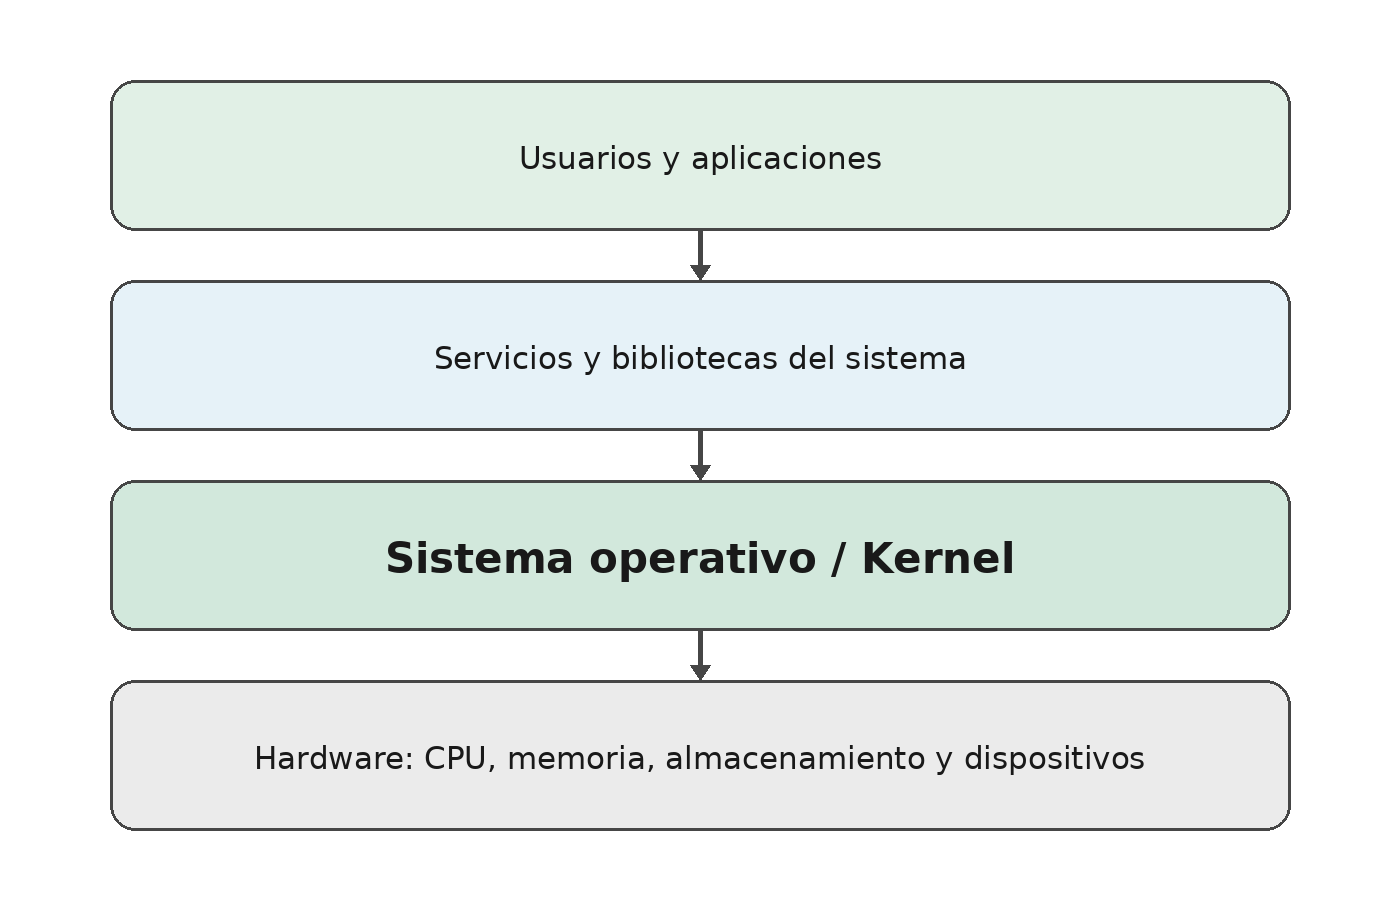
\includegraphics[width=0.88\linewidth,height=\textheight,keepaspectratio]{capitulos/../assets/img/capas_sistema_operativo.png}

}

\caption{Capas principales de un sistema informático}

\end{figure}%

\section{Una comparación sencilla}\label{una-comparaciuxf3n-sencilla}

Pensemos en un hotel:

\begin{itemize}
\tightlist
\item
  Los \textbf{huéspedes} representan a los usuarios y aplicaciones.
\item
  Las \textbf{habitaciones, energía, ascensores y servicios} representan
  los recursos de hardware.
\item
  La \textbf{administración del hotel} representa al sistema operativo.
\end{itemize}

Cada huésped utiliza servicios sin controlar directamente toda la
infraestructura. La administración asigna recursos, organiza
prioridades, establece reglas y evita conflictos.

\begin{tcolorbox}[enhanced jigsaw, arc=.35mm, bottomrule=.15mm, bottomtitle=1mm, breakable, colback=white, colbacktitle=quarto-callout-important-color!10!white, colframe=quarto-callout-important-color-frame, coltitle=black, left=2mm, leftrule=.75mm, opacityback=0, opacitybacktitle=0.6, rightrule=.15mm, title=\textcolor{quarto-callout-important-color}{\faExclamation}\hspace{0.5em}{Importante}, titlerule=0mm, toprule=.15mm, toptitle=1mm]

El sistema operativo no es únicamente la apariencia del escritorio. La
interfaz gráfica es solo una de sus capas. Debajo de ella existen
procesos, controladores, servicios, mecanismos de seguridad y un kernel
que trabaja continuamente.

\end{tcolorbox}

\bookmarksetup{startatroot}

\chapter{El kernel: núcleo del sistema
operativo}\label{el-kernel-nuxfacleo-del-sistema-operativo}

El \textbf{kernel} es la parte central del sistema operativo. Se ejecuta
con privilegios elevados y controla el acceso a los recursos esenciales
del computador.

Entre sus responsabilidades se encuentran:

\begin{itemize}
\tightlist
\item
  planificar el uso del procesador;
\item
  administrar la memoria;
\item
  controlar dispositivos mediante controladores;
\item
  coordinar operaciones de entrada y salida;
\item
  aplicar mecanismos de protección;
\item
  ofrecer servicios a los programas mediante llamadas al sistema.
\end{itemize}

El kernel no debe confundirse con todo el sistema operativo. Un sistema
completo también incluye bibliotecas, utilidades, servicios,
herramientas administrativas e interfaces de usuario.

\section{Modo usuario y modo
privilegiado}\label{modo-usuario-y-modo-privilegiado}

Los procesadores modernos permiten separar al menos dos niveles de
ejecución:

{\def\LTcaptype{none} % do not increment counter
\begin{longtable}[]{@{}
  >{\raggedright\arraybackslash}p{(\linewidth - 4\tabcolsep) * \real{0.3333}}
  >{\raggedright\arraybackslash}p{(\linewidth - 4\tabcolsep) * \real{0.3333}}
  >{\raggedright\arraybackslash}p{(\linewidth - 4\tabcolsep) * \real{0.3333}}@{}}
\toprule\noalign{}
\begin{minipage}[b]{\linewidth}\raggedright
Nivel
\end{minipage} & \begin{minipage}[b]{\linewidth}\raggedright
Característica principal
\end{minipage} & \begin{minipage}[b]{\linewidth}\raggedright
Ejemplo
\end{minipage} \\
\midrule\noalign{}
\endhead
\bottomrule\noalign{}
\endlastfoot
Modo usuario & Acceso limitado; las aplicaciones no controlan
directamente todo el hardware & Navegador, editor de texto,
reproductor \\
Modo kernel o privilegiado & Acceso a operaciones críticas y recursos
protegidos & Kernel, controladores y componentes esenciales \\
\end{longtable}
}

Esta separación evita que un error común en una aplicación tenga acceso
irrestricto a toda la memoria o a los dispositivos del sistema.

\begin{tcolorbox}[enhanced jigsaw, arc=.35mm, bottomrule=.15mm, bottomtitle=1mm, breakable, colback=white, colbacktitle=quarto-callout-warning-color!10!white, colframe=quarto-callout-warning-color-frame, coltitle=black, left=2mm, leftrule=.75mm, opacityback=0, opacitybacktitle=0.6, rightrule=.15mm, title=\textcolor{quarto-callout-warning-color}{\faExclamationTriangle}\hspace{0.5em}{Error común}, titlerule=0mm, toprule=.15mm, toptitle=1mm]

Decir que una aplicación ``habla directamente con el hardware'' suele
ser una simplificación. En la mayoría de los casos, la aplicación
solicita servicios al sistema operativo, y este coordina la operación
con el hardware.

\end{tcolorbox}

\bookmarksetup{startatroot}

\chapter{Funciones principales de un sistema
operativo}\label{funciones-principales-de-un-sistema-operativo}

\section{Gestión de procesos}\label{gestiuxf3n-de-procesos}

Un \textbf{proceso} es un programa en ejecución. El sistema operativo
debe decidir:

\begin{itemize}
\tightlist
\item
  qué proceso utiliza el procesador;
\item
  durante cuánto tiempo;
\item
  cuándo se pausa;
\item
  cuándo continúa;
\item
  y cómo se comunica con otros procesos.
\end{itemize}

Cuando una persona abre un navegador, un editor y una videollamada, el
equipo parece ejecutar todo simultáneamente. En realidad, el sistema
operativo distribuye el tiempo del procesador entre muchas actividades,
aprovechando además los múltiples núcleos de la CPU.

\section{Gestión de memoria}\label{gestiuxf3n-de-memoria}

El sistema operativo asigna memoria a cada proceso y procura que una
aplicación no modifique sin autorización la memoria de otra.

También puede utilizar \textbf{memoria virtual}, una técnica que permite
organizar el espacio de direcciones de los procesos y, cuando es
necesario, apoyar temporalmente la memoria física con almacenamiento
secundario.

\section{Gestión de archivos y
almacenamiento}\label{gestiuxf3n-de-archivos-y-almacenamiento}

El sistema operativo organiza la información mediante archivos,
carpetas, permisos y sistemas de archivos.

Entre sus tareas se encuentran:

\begin{itemize}
\tightlist
\item
  crear, leer, modificar y eliminar archivos;
\item
  organizar directorios;
\item
  controlar permisos;
\item
  registrar ubicaciones y metadatos;
\item
  coordinar el uso de discos, memorias USB y otras unidades.
\end{itemize}

\section{Gestión de dispositivos}\label{gestiuxf3n-de-dispositivos}

Los dispositivos poseen características distintas. Para utilizarlos, el
sistema operativo emplea \textbf{controladores} o \emph{drivers}.

Un controlador traduce solicitudes generales del sistema a operaciones
específicas del dispositivo. Gracias a esta capa, una aplicación puede
imprimir sin conocer todos los detalles internos de cada impresora.

\section{Seguridad y protección}\label{seguridad-y-protecciuxf3n}

El sistema operativo administra usuarios, sesiones, permisos,
credenciales y aislamiento entre procesos.

La seguridad no consiste únicamente en utilizar una contraseña. También
incluye:

\begin{itemize}
\tightlist
\item
  controlar quién puede acceder a un archivo;
\item
  limitar privilegios;
\item
  proteger la memoria;
\item
  aplicar actualizaciones;
\item
  registrar eventos;
\item
  bloquear operaciones no autorizadas.
\end{itemize}

\section{Redes y comunicación}\label{redes-y-comunicaciuxf3n}

Los sistemas operativos modernos incluyen una pila de red que permite
utilizar protocolos, interfaces, puertos y servicios de comunicación.

Cuando un navegador accede a una página web, el sistema operativo
participa en la resolución de nombres, el envío de paquetes, la
recepción de información y la entrega de datos a la aplicación
correspondiente.

\begin{tcolorbox}[enhanced jigsaw, arc=.35mm, bottomrule=.15mm, bottomtitle=1mm, breakable, colback=white, colbacktitle=quarto-callout-tip-color!10!white, colframe=quarto-callout-tip-color-frame, coltitle=black, left=2mm, leftrule=.75mm, opacityback=0, opacitybacktitle=0.6, rightrule=.15mm, title=\textcolor{quarto-callout-tip-color}{\faLightbulb}\hspace{0.5em}{En la práctica profesional}, titlerule=0mm, toprule=.15mm, toptitle=1mm]

Cuando un servidor deja de responder, un administrador no debería
comenzar reinstalando el sistema operativo. Primero revisa el uso de
CPU, memoria, disco, red, procesos y registros para identificar la causa
del problema.

\end{tcolorbox}

\bookmarksetup{startatroot}

\chapter{Breve evolución de los sistemas
operativos}\label{breve-evoluciuxf3n-de-los-sistemas-operativos}

La evolución de los sistemas operativos está estrechamente relacionada
con la evolución del hardware y las necesidades de los usuarios.

\section{Primeras computadoras}\label{primeras-computadoras}

En las primeras generaciones, los programas se cargaban manualmente y el
operador controlaba gran parte del proceso. El tiempo de la computadora
era costoso y se perdía mucho tiempo preparando cada trabajo.

\section{Monitor residente}\label{monitor-residente}

El \textbf{monitor residente} permanecía en memoria y automatizaba parte
de la carga y ejecución de programas. Fue un paso inicial hacia la
coordinación automática de trabajos.

\section{Procesamiento por lotes}\label{procesamiento-por-lotes}

El procesamiento por lotes agrupó varios trabajos para ejecutarlos
secuencialmente con poca interacción humana. Esta modalidad mejoró la
utilización del equipo, aunque el usuario debía esperar para recibir
resultados.

\section{Multiprogramación y tiempo
compartido}\label{multiprogramaciuxf3n-y-tiempo-compartido}

La multiprogramación permitió mantener varios trabajos en memoria y
utilizar el procesador mientras otro esperaba una operación de entrada o
salida.

El tiempo compartido extendió esta idea para atender a varios usuarios
de forma interactiva, ofreciendo la impresión de que cada uno disponía
del sistema.

\section{Computadoras personales e interfaces
gráficas}\label{computadoras-personales-e-interfaces-gruxe1ficas}

Las computadoras personales acercaron la informática a hogares y
oficinas. Las interfaces gráficas facilitaron el uso mediante ventanas,
iconos, menús y dispositivos apuntadores.

\section{Internet, dispositivos móviles, nube y
virtualización}\label{internet-dispositivos-muxf3viles-nube-y-virtualizaciuxf3n}

Los sistemas actuales ya no se limitan a una computadora de escritorio.
Existen sistemas para:

\begin{itemize}
\tightlist
\item
  servidores físicos y virtuales;
\item
  teléfonos y tabletas;
\item
  dispositivos integrados;
\item
  infraestructura en la nube;
\item
  vehículos y equipos industriales;
\item
  plataformas de contenedores.
\end{itemize}

\begin{tcolorbox}[enhanced jigsaw, arc=.35mm, bottomrule=.15mm, bottomtitle=1mm, breakable, colback=white, colbacktitle=quarto-callout-note-color!10!white, colframe=quarto-callout-note-color-frame, coltitle=black, left=2mm, leftrule=.75mm, opacityback=0, opacitybacktitle=0.6, rightrule=.15mm, title=\textcolor{quarto-callout-note-color}{\faInfo}\hspace{0.5em}{Perspectiva histórica}, titlerule=0mm, toprule=.15mm, toptitle=1mm]

Los sistemas antiguos como MS-DOS, Windows XP o las primeras versiones
de Mac OS siguen siendo importantes para comprender la evolución, pero
no deben presentarse como el panorama tecnológico actual.

\end{tcolorbox}

\bookmarksetup{startatroot}

\chapter{Panorama actual de sistemas
operativos}\label{panorama-actual-de-sistemas-operativos}

La siguiente tabla presenta familias relevantes para un estudiante de
Ingeniería en Sistemas.

{\def\LTcaptype{none} % do not increment counter
\begin{longtable}[]{@{}
  >{\raggedright\arraybackslash}p{(\linewidth - 4\tabcolsep) * \real{0.3333}}
  >{\raggedright\arraybackslash}p{(\linewidth - 4\tabcolsep) * \real{0.3333}}
  >{\raggedright\arraybackslash}p{(\linewidth - 4\tabcolsep) * \real{0.3333}}@{}}
\toprule\noalign{}
\begin{minipage}[b]{\linewidth}\raggedright
Familia
\end{minipage} & \begin{minipage}[b]{\linewidth}\raggedright
Uso frecuente
\end{minipage} & \begin{minipage}[b]{\linewidth}\raggedright
Característica general
\end{minipage} \\
\midrule\noalign{}
\endhead
\bottomrule\noalign{}
\endlastfoot
Windows & Equipos personales, organizaciones y estaciones de trabajo &
Amplio ecosistema comercial y compatibilidad de aplicaciones \\
Windows Server & Servidores empresariales & Servicios de red,
identidades, virtualización y administración centralizada \\
GNU/Linux & Servidores, nube, desarrollo, escritorio, supercomputación y
sistemas integrados & Código abierto, variedad de distribuciones y gran
capacidad de automatización \\
macOS & Computadoras Mac & Integración estrecha entre hardware y
software de Apple \\
Android & Teléfonos, tabletas, televisores y dispositivos & Plataforma
móvil basada en el kernel Linux \\
iOS/iPadOS & iPhone y iPad & Integración con el ecosistema y hardware de
Apple \\
Sistemas de tiempo real & Industria, vehículos, telecomunicaciones y
control & Respuesta predecible dentro de límites temporales \\
\end{longtable}
}

\section{Windows y Windows Server}\label{windows-y-windows-server}

A julio de 2026, Windows 11 continúa como la familia principal de
escritorio de Microsoft. Microsoft mantiene información oficial de
versiones y canales de actualización en su portal de salud de versiones.
Windows Server 2025 es la versión LTSC vigente de la plataforma de
servidores y se orienta a seguridad, virtualización, almacenamiento e
integración híbrida.

La línea de tiempo incluida en el material original muestra parte de la
evolución de Windows. Se conserva como referencia histórica, pero debe
leerse junto con la información actualizada de esta sección.

\begin{figure}[H]

{\centering 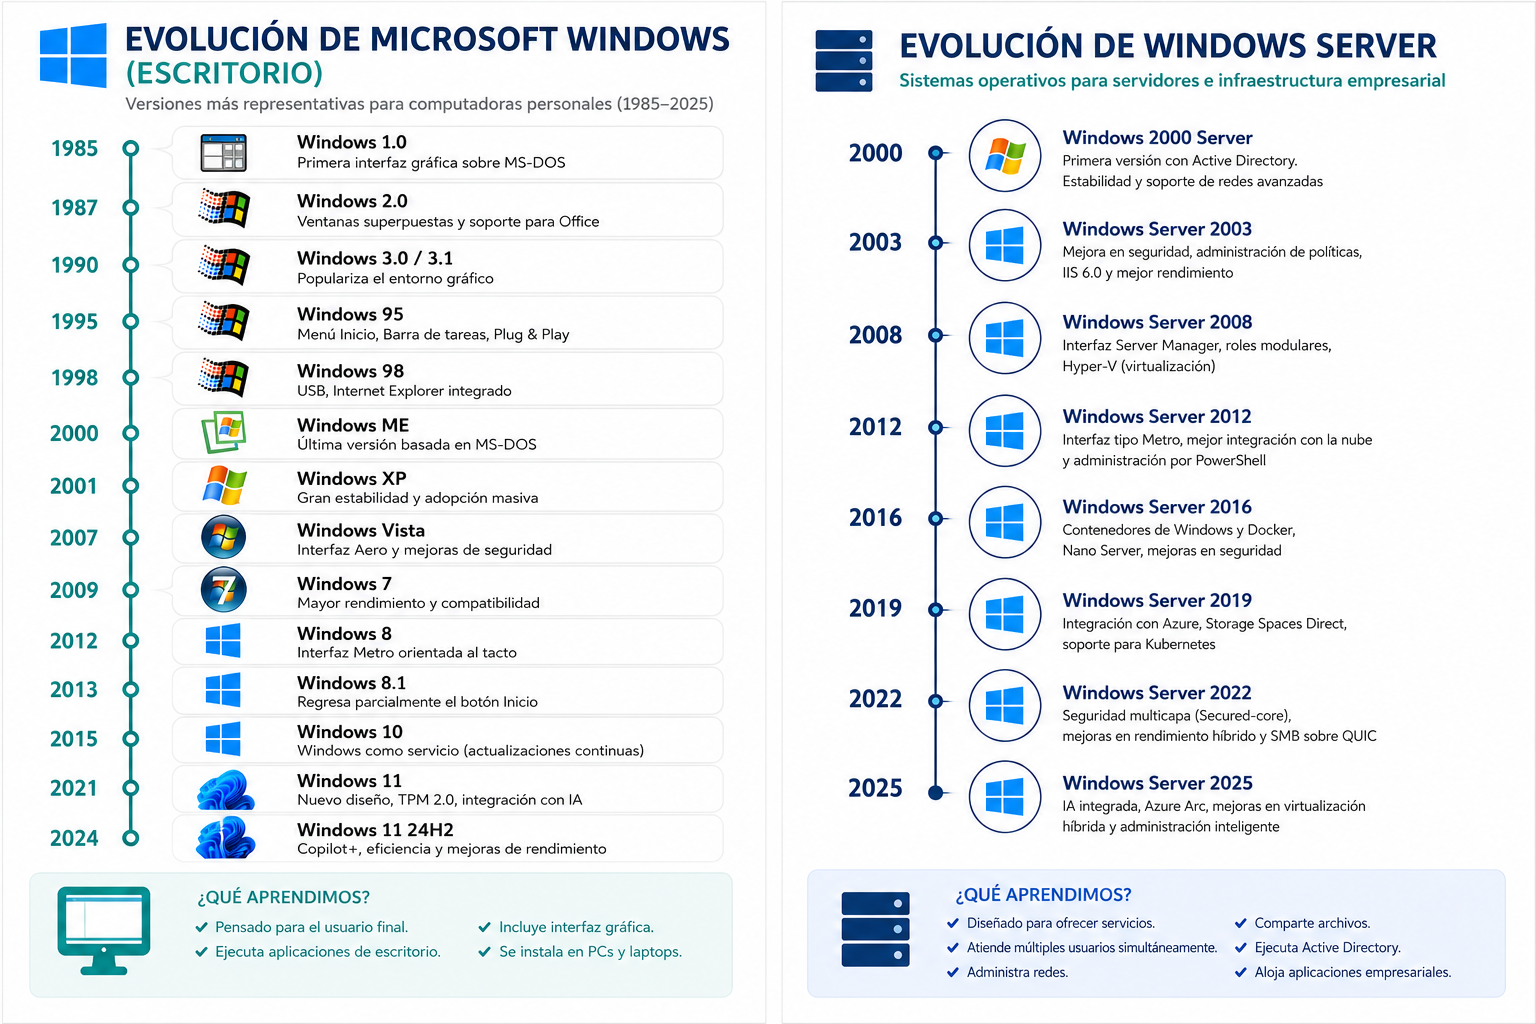
\includegraphics[width=0.82\linewidth,height=\textheight,keepaspectratio]{capitulos/../assets/img/linea_tiempo_windows_material_original.png}

}

\caption{Evolución de Windows en el material original de la clase}

\end{figure}%

\section{GNU/Linux}\label{gnulinux}

Linux es el kernel iniciado por Linus Torvalds. Cuando se combina con
herramientas, bibliotecas, gestores de paquetes y entornos de usuario,
forma sistemas completos distribuidos en variantes como Ubuntu, Debian,
Fedora, Rocky Linux, AlmaLinux o Arch Linux.

Ubuntu 24.04 LTS continúa siendo una versión de soporte prolongado
ampliamente utilizada. Las versiones LTS priorizan estabilidad y
mantenimiento extendido, una característica valiosa en organizaciones y
servidores.

\begin{tcolorbox}[enhanced jigsaw, arc=.35mm, bottomrule=.15mm, bottomtitle=1mm, breakable, colback=white, colbacktitle=quarto-callout-important-color!10!white, colframe=quarto-callout-important-color-frame, coltitle=black, left=2mm, leftrule=.75mm, opacityback=0, opacitybacktitle=0.6, rightrule=.15mm, title=\textcolor{quarto-callout-important-color}{\faExclamation}\hspace{0.5em}{Precisión terminológica}, titlerule=0mm, toprule=.15mm, toptitle=1mm]

Linux es técnicamente el kernel. En el uso cotidiano se habla de
``sistema operativo Linux'', pero una expresión más precisa para muchas
distribuciones es GNU/Linux o simplemente el nombre de la distribución:
Ubuntu, Debian, Fedora, etc.

\end{tcolorbox}

\section{macOS}\label{macos}

macOS es el sistema operativo de las computadoras Mac. A julio de 2026,
macOS Tahoe 26 es la versión estable con actualizaciones de seguridad
publicadas por Apple; macOS 27 se encuentra anunciado o en ciclo previo
a su disponibilidad general según el momento de consulta.

Para un libro reutilizable es preferible enseñar la familia, su
arquitectura general y sus herramientas, en lugar de depender únicamente
del número de versión.

\section{Android e iOS}\label{android-e-ios}

Android domina una gran variedad de dispositivos móviles y utiliza el
kernel Linux como base, aunque su entorno de aplicaciones y servicios es
diferente al de una distribución GNU/Linux de escritorio.

Android 17 fue publicado en junio de 2026. En el ecosistema Apple, iOS
26 continúa como versión estable con actualizaciones de seguridad,
mientras iOS 27 fue anunciado para una etapa posterior.

\begin{tcolorbox}[enhanced jigsaw, arc=.35mm, bottomrule=.15mm, bottomtitle=1mm, breakable, colback=white, colbacktitle=quarto-callout-tip-color!10!white, colframe=quarto-callout-tip-color-frame, coltitle=black, left=2mm, leftrule=.75mm, opacityback=0, opacitybacktitle=0.6, rightrule=.15mm, title=\textcolor{quarto-callout-tip-color}{\faLightbulb}\hspace{0.5em}{Consejo del Ingeniero}, titlerule=0mm, toprule=.15mm, toptitle=1mm]

Las versiones cambian con rapidez. En la práctica profesional, siempre
consulte la documentación oficial antes de planificar una instalación,
una actualización o una migración.

\end{tcolorbox}

\bookmarksetup{startatroot}

\chapter{Interfaces de usuario}\label{interfaces-de-usuario}

Una interfaz permite que una persona interactúe con el sistema
operativo.

\section{Interfaz gráfica de
usuario}\label{interfaz-gruxe1fica-de-usuario}

La \textbf{GUI} (\emph{Graphical User Interface}) utiliza ventanas,
iconos, menús, botones y otros elementos visuales.

Sus ventajas incluyen:

\begin{itemize}
\tightlist
\item
  facilidad de aprendizaje;
\item
  descubrimiento visual de opciones;
\item
  interacción mediante mouse, pantalla táctil o teclado;
\item
  buena experiencia para tareas generales.
\end{itemize}

\section{Interfaz de línea de
comandos}\label{interfaz-de-luxednea-de-comandos}

La \textbf{CLI} (\emph{Command-Line Interface}) permite escribir
instrucciones en una terminal o intérprete de comandos.

Entre sus ventajas se encuentran:

\begin{itemize}
\tightlist
\item
  automatización mediante scripts;
\item
  administración remota;
\item
  precisión y repetibilidad;
\item
  menor consumo de recursos en muchos escenarios;
\item
  acceso rápido a herramientas avanzadas.
\end{itemize}

\begin{figure}[H]

{\centering 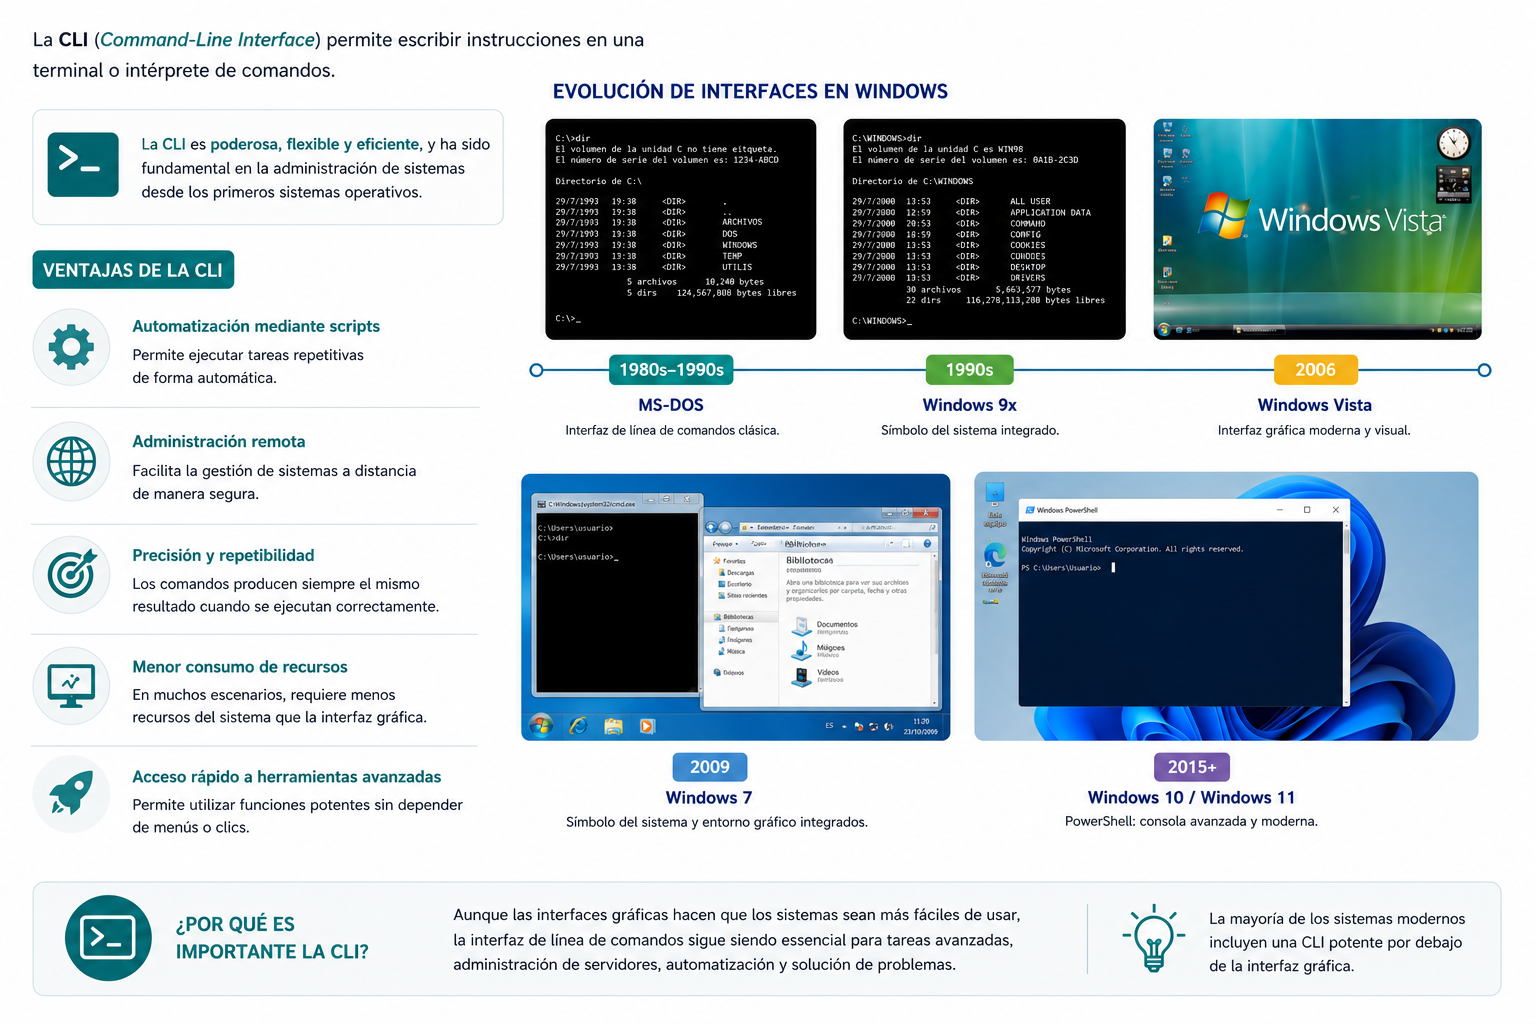
\includegraphics[width=0.85\linewidth,height=\textheight,keepaspectratio]{capitulos/../assets/img/interfaces_material_original.png}

}

\caption{Ejemplos de interfaces conservados del material original}

\end{figure}%

\section{No son enemigas}\label{no-son-enemigas}

GUI y CLI no deben verse como opciones excluyentes. Un profesional
utiliza ambas según la tarea.

{\def\LTcaptype{none} % do not increment counter
\begin{longtable}[]{@{}ll@{}}
\toprule\noalign{}
Situación & Interfaz conveniente \\
\midrule\noalign{}
\endhead
\bottomrule\noalign{}
\endlastfoot
Configurar una opción ocasional & GUI \\
Repetir la misma tarea en 100 equipos & CLI y automatización \\
Explorar visualmente archivos & GUI \\
Administrar un servidor remoto & CLI \\
Analizar procesos rápidamente & GUI o CLI, según el contexto \\
\end{longtable}
}

\begin{tcolorbox}[enhanced jigsaw, arc=.35mm, bottomrule=.15mm, bottomtitle=1mm, breakable, colback=white, colbacktitle=quarto-callout-tip-color!10!white, colframe=quarto-callout-tip-color-frame, coltitle=black, left=2mm, leftrule=.75mm, opacityback=0, opacitybacktitle=0.6, rightrule=.15mm, title=\textcolor{quarto-callout-tip-color}{\faLightbulb}\hspace{0.5em}{En la práctica profesional}, titlerule=0mm, toprule=.15mm, toptitle=1mm]

PowerShell, Bash y otras shells permiten convertir procedimientos
manuales en scripts repetibles. Esa capacidad reduce errores y facilita
administrar muchos equipos.

\end{tcolorbox}

\bookmarksetup{startatroot}

\chapter{Clasificación de los sistemas
operativos}\label{clasificaciuxf3n-de-los-sistemas-operativos}

Un sistema operativo puede pertenecer a varias categorías al mismo
tiempo.

\section{Monotarea y multitarea}\label{monotarea-y-multitarea}

\begin{itemize}
\tightlist
\item
  \textbf{Monotarea:} ejecuta una tarea principal a la vez.
\item
  \textbf{Multitarea:} administra varios procesos concurrentes y
  distribuye recursos entre ellos.
\end{itemize}

Los sistemas generales actuales son multitarea.

\section{Monousuario y multiusuario}\label{monousuario-y-multiusuario}

\begin{itemize}
\tightlist
\item
  \textbf{Monousuario:} está diseñado principalmente para una sesión o
  usuario a la vez.
\item
  \textbf{Multiusuario:} permite atender varios usuarios y separar
  recursos, permisos y sesiones.
\end{itemize}

Un servidor Linux o Windows Server puede atender múltiples usuarios y
servicios simultáneamente.

\section{Procesamiento por lotes}\label{procesamiento-por-lotes-1}

Ejecuta conjuntos de trabajos con poca interacción durante el
procesamiento. Sigue siendo útil en tareas como generación nocturna de
reportes, respaldo de información o procesamiento masivo de datos.

\section{Tiempo compartido}\label{tiempo-compartido}

Distribuye el tiempo de CPU entre múltiples usuarios o procesos
interactivos, proporcionando respuestas suficientemente rápidas para
mantener la sensación de atención individual.

\section{Sistemas de red y
distribuidos}\label{sistemas-de-red-y-distribuidos}

Un sistema operativo de red facilita compartir servicios y recursos
entre equipos conectados. Un sistema distribuido coordina componentes
ubicados en diferentes nodos para ofrecer un servicio integrado.

\section{Sistemas de tiempo real}\label{sistemas-de-tiempo-real}

Un sistema de tiempo real debe responder dentro de límites temporales
definidos.

\begin{itemize}
\tightlist
\item
  \textbf{Tiempo real duro:} incumplir el plazo puede producir una falla
  crítica.
\item
  \textbf{Tiempo real blando:} el retraso reduce la calidad del
  servicio, pero no necesariamente causa una falla catastrófica.
\end{itemize}

Ejemplos:

\begin{itemize}
\tightlist
\item
  control industrial;
\item
  sistemas automotrices;
\item
  telecomunicaciones;
\item
  robótica;
\item
  instrumentación médica;
\item
  control de energía.
\end{itemize}

\begin{figure}[H]

{\centering 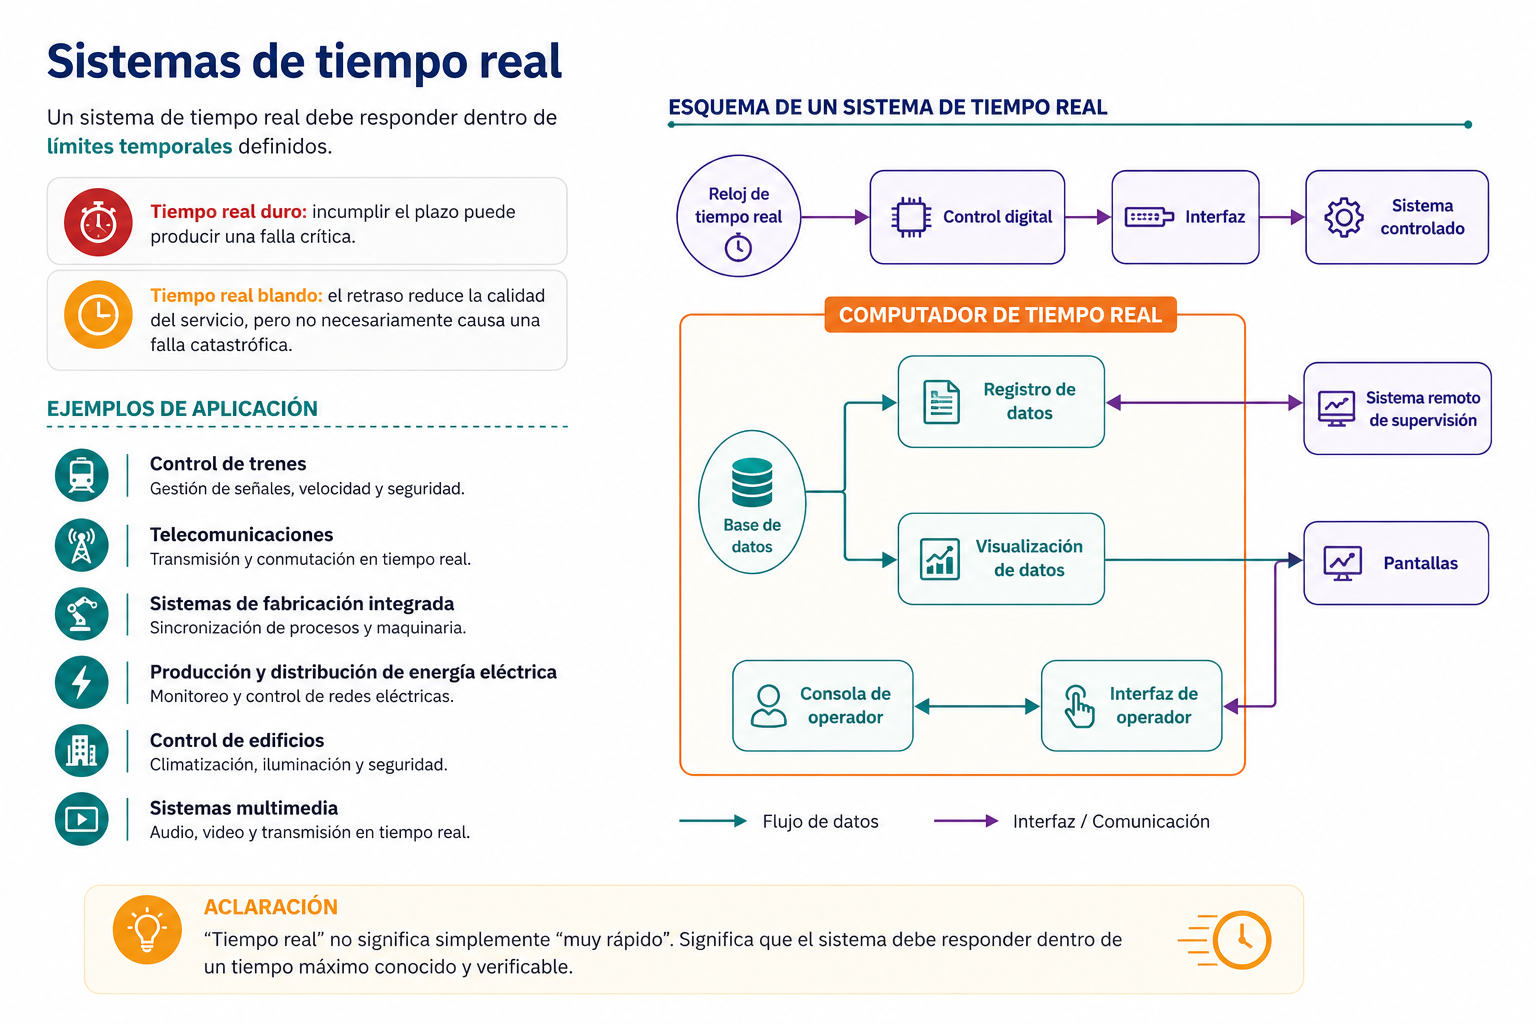
\includegraphics[width=0.72\linewidth,height=\textheight,keepaspectratio]{capitulos/../assets/img/sistema_tiempo_real_material_original.png}

}

\caption{Esquema de sistema de tiempo real tomado del material original}

\end{figure}%

\begin{tcolorbox}[enhanced jigsaw, arc=.35mm, bottomrule=.15mm, bottomtitle=1mm, breakable, colback=white, colbacktitle=quarto-callout-warning-color!10!white, colframe=quarto-callout-warning-color-frame, coltitle=black, left=2mm, leftrule=.75mm, opacityback=0, opacitybacktitle=0.6, rightrule=.15mm, title=\textcolor{quarto-callout-warning-color}{\faExclamationTriangle}\hspace{0.5em}{Aclaración}, titlerule=0mm, toprule=.15mm, toptitle=1mm]

``Tiempo real'' no significa simplemente ``muy rápido''. Significa que
el sistema debe responder dentro de un tiempo máximo conocido y
verificable.

\end{tcolorbox}

\bookmarksetup{startatroot}

\chapter{Llamadas al sistema}\label{llamadas-al-sistema}

Las aplicaciones necesitan solicitar servicios al kernel. Para hacerlo
utilizan \textbf{llamadas al sistema}.

Algunos servicios típicos son:

\begin{itemize}
\tightlist
\item
  abrir o cerrar un archivo;
\item
  crear un proceso;
\item
  reservar memoria;
\item
  comunicarse por red;
\item
  leer datos de un dispositivo;
\item
  consultar la hora del sistema.
\end{itemize}

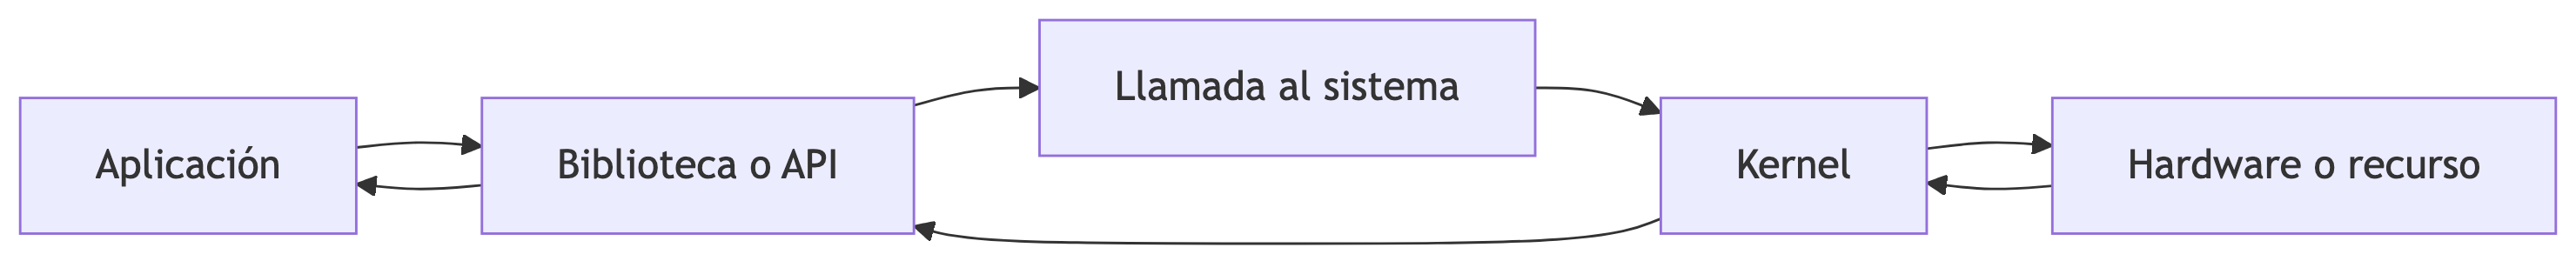
\includegraphics[width=10.68in,height=1.09in]{capitulos/01_introduccion_sistemas_operativos_files/figure-latex/mermaid-figure-1.png}

\section{Bibliotecas y API}\label{bibliotecas-y-api}

Los lenguajes de alto nivel suelen utilizar bibliotecas que presentan
funciones más sencillas. La biblioteca prepara los parámetros y realiza
la transición necesaria para solicitar el servicio al sistema operativo.

Por ejemplo, una aplicación puede llamar una función para abrir un
archivo. Esa función termina utilizando servicios del sistema operativo
para validar permisos, localizar el archivo y coordinar el acceso al
almacenamiento.

\begin{tcolorbox}[enhanced jigsaw, arc=.35mm, bottomrule=.15mm, bottomtitle=1mm, breakable, colback=white, colbacktitle=quarto-callout-note-color!10!white, colframe=quarto-callout-note-color-frame, coltitle=black, left=2mm, leftrule=.75mm, opacityback=0, opacitybacktitle=0.6, rightrule=.15mm, title=\textcolor{quarto-callout-note-color}{\faInfo}\hspace{0.5em}{Observe}, titlerule=0mm, toprule=.15mm, toptitle=1mm]

Las llamadas al sistema forman una frontera controlada entre las
aplicaciones y el kernel. Esta frontera permite ofrecer servicios sin
entregar a cada programa control total sobre el equipo.

\end{tcolorbox}

\bookmarksetup{startatroot}

\chapter{Relación con la arquitectura del
computador}\label{relaciuxf3n-con-la-arquitectura-del-computador}

Para comprender un sistema operativo también necesitamos recordar los
componentes básicos del computador.

\section{CPU}\label{cpu}

La \textbf{unidad central de procesamiento} ejecuta instrucciones y
realiza operaciones aritméticas, lógicas y de control.

En sistemas modernos, una CPU puede incluir varios núcleos, memorias
caché y mecanismos especializados. El sistema operativo planifica
procesos e hilos para aprovechar esos recursos.

\section{Memoria principal}\label{memoria-principal}

La memoria RAM almacena temporalmente instrucciones y datos necesarios
durante la ejecución.

Es rápida, pero normalmente pierde su contenido al apagar el equipo. El
sistema operativo administra qué regiones utiliza cada proceso y
coordina la memoria virtual.

\section{Almacenamiento secundario}\label{almacenamiento-secundario}

SSD, discos duros y otros medios conservan información de forma
persistente. Son más lentos que la RAM, pero poseen mayor capacidad.

\section{Unidad de control y ALU}\label{unidad-de-control-y-alu}

La unidad de control coordina la ejecución de instrucciones dentro del
procesador. La unidad aritmética y lógica realiza operaciones
matemáticas y comparaciones.

En cursos modernos estos componentes se estudian como partes de la
arquitectura del procesador, mientras el sistema operativo se analiza
como el software que administra su utilización.

\section{Periféricos y
entrada/salida}\label{perifuxe9ricos-y-entradasalida}

Teclado, mouse, pantalla, almacenamiento, impresoras y adaptadores de
red intercambian información con el sistema mediante controladores y
mecanismos de entrada/salida.

\begin{tcolorbox}[enhanced jigsaw, arc=.35mm, bottomrule=.15mm, bottomtitle=1mm, breakable, colback=white, colbacktitle=quarto-callout-tip-color!10!white, colframe=quarto-callout-tip-color-frame, coltitle=black, left=2mm, leftrule=.75mm, opacityback=0, opacitybacktitle=0.6, rightrule=.15mm, title=\textcolor{quarto-callout-tip-color}{\faLightbulb}\hspace{0.5em}{Consejo del Ingeniero}, titlerule=0mm, toprule=.15mm, toptitle=1mm]

Cuando una computadora está lenta, no asuma inmediatamente que ``la CPU
está mala''. El cuello de botella puede encontrarse en memoria,
almacenamiento, red, temperatura, controladores o en un proceso
específico.

\end{tcolorbox}

\bookmarksetup{startatroot}

\chapter{Virtualización y contenedores: una mirada
actual}\label{virtualizaciuxf3n-y-contenedores-una-mirada-actual}

La virtualización permite ejecutar máquinas virtuales con su propio
sistema operativo sobre un hipervisor.

Una máquina virtual normalmente incluye:

\begin{itemize}
\tightlist
\item
  un sistema operativo invitado;
\item
  su propio kernel;
\item
  memoria virtual asignada;
\item
  dispositivos virtuales.
\end{itemize}

Los contenedores aíslan procesos y sus dependencias, pero comparten el
kernel del sistema anfitrión. Por eso suelen ser más ligeros que una
máquina virtual completa.

{\def\LTcaptype{none} % do not increment counter
\begin{longtable}[]{@{}
  >{\raggedright\arraybackslash}p{(\linewidth - 4\tabcolsep) * \real{0.3333}}
  >{\raggedright\arraybackslash}p{(\linewidth - 4\tabcolsep) * \real{0.3333}}
  >{\raggedright\arraybackslash}p{(\linewidth - 4\tabcolsep) * \real{0.3333}}@{}}
\toprule\noalign{}
\begin{minipage}[b]{\linewidth}\raggedright
Característica
\end{minipage} & \begin{minipage}[b]{\linewidth}\raggedright
Máquina virtual
\end{minipage} & \begin{minipage}[b]{\linewidth}\raggedright
Contenedor
\end{minipage} \\
\midrule\noalign{}
\endhead
\bottomrule\noalign{}
\endlastfoot
Kernel propio & Sí & Generalmente no; comparte el kernel anfitrión \\
Aislamiento & Alto & A nivel de procesos y recursos \\
Tamaño & Mayor & Menor \\
Inicio & Más lento & Habitualmente rápido \\
Uso típico & Sistemas completos, pruebas de SO, aislamiento fuerte &
Empaquetado y despliegue de aplicaciones \\
\end{longtable}
}

\begin{tcolorbox}[enhanced jigsaw, arc=.35mm, bottomrule=.15mm, bottomtitle=1mm, breakable, colback=white, colbacktitle=quarto-callout-note-color!10!white, colframe=quarto-callout-note-color-frame, coltitle=black, left=2mm, leftrule=.75mm, opacityback=0, opacitybacktitle=0.6, rightrule=.15mm, title=\textcolor{quarto-callout-note-color}{\faInfo}\hspace{0.5em}{Primera aproximación}, titlerule=0mm, toprule=.15mm, toptitle=1mm]

Virtualización y contenedores se estudiarán con mayor profundidad más
adelante. En esta clase basta comprender que ambos dependen de funciones
esenciales del sistema operativo.

\end{tcolorbox}

\bookmarksetup{startatroot}

\chapter{Laboratorio 1: conozca su sistema
operativo}\label{laboratorio-1-conozca-su-sistema-operativo}

\section{Propósito}\label{propuxf3sito}

Identificar el sistema operativo del equipo y relacionar los conceptos
estudiados con información real.

\section{Actividad A: información
general}\label{actividad-a-informaciuxf3n-general}

Registre los siguientes datos:

{\def\LTcaptype{none} % do not increment counter
\begin{longtable}[]{@{}ll@{}}
\toprule\noalign{}
Dato & Resultado de su equipo \\
\midrule\noalign{}
\endhead
\bottomrule\noalign{}
\endlastfoot
Sistema operativo & \\
Edición o distribución & \\
Versión & \\
Arquitectura & \\
Procesador & \\
Memoria RAM & \\
Nombre del equipo & \\
Usuario actual & \\
Espacio disponible & \\
\end{longtable}
}

\section{Actividad B: Windows}\label{actividad-b-windows}

Abra \textbf{Terminal}, \textbf{PowerShell} o \textbf{Símbolo del
sistema} y ejecute:

\begin{Shaded}
\begin{Highlighting}[]
\NormalTok{systeminfo}
\end{Highlighting}
\end{Shaded}

También puede utilizar:

\begin{Shaded}
\begin{Highlighting}[]
\NormalTok{Get{-}ComputerInfo}
\end{Highlighting}
\end{Shaded}

Comandos básicos seguros para explorar:

\begin{Shaded}
\begin{Highlighting}[]
\NormalTok{hostname}
\NormalTok{whoami}
\FunctionTok{Get{-}Location}
\FunctionTok{Get{-}ChildItem}
\end{Highlighting}
\end{Shaded}

Responda:

\begin{enumerate}
\def\labelenumi{\arabic{enumi}.}
\tightlist
\item
  ¿Qué versión y compilación de Windows utiliza?
\item
  ¿Cuánta memoria física aparece instalada?
\item
  ¿Cuál es el nombre del equipo?
\item
  ¿Qué diferencia observa entre \texttt{Get-ChildItem} y la vista del
  Explorador de archivos?
\end{enumerate}

\section{Actividad C: macOS}\label{actividad-c-macos}

Abra \textbf{Terminal} y ejecute:

\begin{Shaded}
\begin{Highlighting}[]
\ExtensionTok{sw\_vers}
\FunctionTok{uname} \AttributeTok{{-}a}
\FunctionTok{whoami}
\FunctionTok{hostname}
\BuiltInTok{pwd}
\FunctionTok{ls}
\ExtensionTok{system\_profiler}\NormalTok{ SPHardwareDataType}
\end{Highlighting}
\end{Shaded}

Responda:

\begin{enumerate}
\def\labelenumi{\arabic{enumi}.}
\tightlist
\item
  ¿Qué versión de macOS utiliza?
\item
  ¿Qué arquitectura reporta el equipo?
\item
  ¿Qué información muestra \texttt{pwd}?
\item
  ¿Qué relación encuentra entre Finder y \texttt{ls}?
\end{enumerate}

\section{Actividad D: GNU/Linux}\label{actividad-d-gnulinux}

Abra una terminal y ejecute:

\begin{Shaded}
\begin{Highlighting}[]
\FunctionTok{cat}\NormalTok{ /etc/os{-}release}
\FunctionTok{uname} \AttributeTok{{-}r}
\ExtensionTok{hostnamectl}
\FunctionTok{whoami}
\BuiltInTok{pwd}
\FunctionTok{ls}
\end{Highlighting}
\end{Shaded}

Responda:

\begin{enumerate}
\def\labelenumi{\arabic{enumi}.}
\tightlist
\item
  ¿Cuál es la distribución?
\item
  ¿Qué versión del kernel utiliza?
\item
  ¿Qué arquitectura tiene el equipo?
\item
  ¿Qué información proporciona \texttt{/etc/os-release}?
\end{enumerate}

\section{Actividad E: comparación}\label{actividad-e-comparaciuxf3n}

Complete la tabla:

{\def\LTcaptype{none} % do not increment counter
\begin{longtable}[]{@{}
  >{\raggedright\arraybackslash}p{(\linewidth - 4\tabcolsep) * \real{0.3333}}
  >{\raggedright\arraybackslash}p{(\linewidth - 4\tabcolsep) * \real{0.3333}}
  >{\raggedright\arraybackslash}p{(\linewidth - 4\tabcolsep) * \real{0.3333}}@{}}
\toprule\noalign{}
\begin{minipage}[b]{\linewidth}\raggedright
Acción
\end{minipage} & \begin{minipage}[b]{\linewidth}\raggedright
Windows
\end{minipage} & \begin{minipage}[b]{\linewidth}\raggedright
macOS/Linux
\end{minipage} \\
\midrule\noalign{}
\endhead
\bottomrule\noalign{}
\endlastfoot
Mostrar usuario & \texttt{whoami} & \texttt{whoami} \\
Mostrar nombre del equipo & \texttt{hostname} & \texttt{hostname} \\
Mostrar carpeta actual & \texttt{Get-Location} & \texttt{pwd} \\
Listar archivos & \texttt{Get-ChildItem} & \texttt{ls} \\
Información del sistema & \texttt{systeminfo} & \texttt{sw\_vers},
\texttt{hostnamectl} o \texttt{/etc/os-release} \\
\end{longtable}
}

\begin{tcolorbox}[enhanced jigsaw, arc=.35mm, bottomrule=.15mm, bottomtitle=1mm, breakable, colback=white, colbacktitle=quarto-callout-warning-color!10!white, colframe=quarto-callout-warning-color-frame, coltitle=black, left=2mm, leftrule=.75mm, opacityback=0, opacitybacktitle=0.6, rightrule=.15mm, title=\textcolor{quarto-callout-warning-color}{\faExclamationTriangle}\hspace{0.5em}{Regla del laboratorio}, titlerule=0mm, toprule=.15mm, toptitle=1mm]

Ejecute únicamente los comandos indicados y lea su salida. No modifique
usuarios, permisos, particiones, fecha, hora ni configuraciones del
sistema durante esta práctica.

\end{tcolorbox}

\bookmarksetup{startatroot}

\chapter{Caso de análisis}\label{caso-de-anuxe1lisis}

Una empresa posee:

\begin{itemize}
\tightlist
\item
  40 computadoras de oficina;
\item
  un servidor de archivos;
\item
  una aplicación web;
\item
  teléfonos utilizados por personal de campo;
\item
  un sistema industrial que debe responder en milisegundos.
\end{itemize}

Analice qué tipo de sistema operativo podría utilizarse en cada contexto
y justifique su respuesta considerando:

\begin{itemize}
\tightlist
\item
  propósito;
\item
  seguridad;
\item
  administración;
\item
  interfaz;
\item
  tiempo de respuesta;
\item
  compatibilidad de aplicaciones.
\end{itemize}

\bookmarksetup{startatroot}

\chapter{Resumen de la clase}\label{resumen-de-la-clase}

En esta clase aprendimos que:

\begin{itemize}
\tightlist
\item
  El sistema operativo administra hardware y ofrece servicios a las
  aplicaciones.
\item
  El kernel es el núcleo privilegiado del sistema.
\item
  Los procesos, la memoria, los archivos, los dispositivos, la seguridad
  y la red son recursos administrados por el sistema operativo.
\item
  GUI y CLI son formas complementarias de interacción.
\item
  Los sistemas operativos pueden clasificarse por su número de tareas,
  usuarios, forma de procesamiento y requisitos temporales.
\item
  Las llamadas al sistema permiten a las aplicaciones solicitar
  servicios al kernel.
\item
  Windows, GNU/Linux, macOS, Android, iOS y los sistemas de tiempo real
  responden a necesidades distintas.
\item
  La virtualización y los contenedores dependen de capacidades
  fundamentales del sistema operativo.
\end{itemize}

\begin{tcolorbox}[enhanced jigsaw, arc=.35mm, bottomrule=.15mm, bottomtitle=1mm, breakable, colback=white, colbacktitle=quarto-callout-tip-color!10!white, colframe=quarto-callout-tip-color-frame, coltitle=black, left=2mm, leftrule=.75mm, opacityback=0, opacitybacktitle=0.6, rightrule=.15mm, title=\textcolor{quarto-callout-tip-color}{\faLightbulb}\hspace{0.5em}{Consejo final del Ingeniero}, titlerule=0mm, toprule=.15mm, toptitle=1mm]

Un buen administrador no memoriza únicamente comandos. Comprende qué
recurso está observando, qué problema intenta resolver y qué efecto
tendrá cada acción.

\end{tcolorbox}

\bookmarksetup{startatroot}

\chapter{Tarea sugerida}\label{tarea-sugerida}

\begin{enumerate}
\def\labelenumi{\arabic{enumi}.}
\tightlist
\item
  Elabore una comparación entre el sistema operativo de su computadora y
  el de su teléfono.
\item
  Identifique tres procesos activos en su equipo y explique, con sus
  propias palabras, para qué sirven.
\item
  Explique la diferencia entre kernel, sistema operativo e interfaz
  gráfica.
\item
  Investigue un ejemplo de sistema de tiempo real y explique por qué el
  cumplimiento del tiempo es importante.
\item
  Describa una situación en la que utilizaría una máquina virtual y otra
  en la que utilizaría un contenedor.
\item
  Incluya capturas de pantalla de la información obtenida en el
  laboratorio, ocultando datos personales que no desee compartir.
\end{enumerate}

\bookmarksetup{startatroot}

\chapter{Fuentes oficiales para
actualización}\label{fuentes-oficiales-para-actualizaciuxf3n}

\begin{itemize}
\tightlist
\item
  Microsoft. \emph{Windows 11 release information}:
  \url{https://learn.microsoft.com/windows/release-health/windows11-release-information}
\item
  Microsoft. \emph{Windows Server release information}:
  \url{https://learn.microsoft.com/windows/release-health/windows-server-release-info}
\item
  Apple. \emph{Apple security releases}:
  \url{https://support.apple.com/100100}
\item
  Canonical. \emph{Ubuntu release cycle}:
  \url{https://ubuntu.com/about/release-cycle}
\item
  Linux Kernel Organization. \emph{The Linux Kernel Archives}:
  \url{https://www.kernel.org/}
\item
  Android Developers. \emph{Android platform updates}:
  \url{https://developer.android.com/latest-updates}
\item
  Docker. \emph{What is a container?}:
  \url{https://docs.docker.com/get-started/docker-concepts/the-basics/what-is-a-container/}
\end{itemize}

\begin{tcolorbox}[enhanced jigsaw, arc=.35mm, bottomrule=.15mm, bottomtitle=1mm, breakable, colback=white, colbacktitle=quarto-callout-note-color!10!white, colframe=quarto-callout-note-color-frame, coltitle=black, left=2mm, leftrule=.75mm, opacityback=0, opacitybacktitle=0.6, rightrule=.15mm, title=\textcolor{quarto-callout-note-color}{\faInfo}\hspace{0.5em}{Nota editorial}, titlerule=0mm, toprule=.15mm, toptitle=1mm]

La información de versiones fue revisada en julio de 2026. Debido a que
los sistemas operativos se actualizan continuamente, las versiones
exactas deben verificarse en la documentación oficial al impartir
nuevamente la clase.

\end{tcolorbox}

\bookmarksetup{startatroot}

\chapter{Administración del sistema de archivos desde la línea de
comandos}\label{administraciuxf3n-del-sistema-de-archivos-desde-la-luxednea-de-comandos}

Clase 2

\hfill\break

\bookmarksetup{startatroot}

\chapter{Presentación de la clase}\label{presentaciuxf3n-de-la-clase-1}

En la clase anterior estudiamos qué es un sistema operativo y por qué
constituye la base de todo sistema informático. En esta sesión nos
concentraremos en una de sus funciones más visibles: \textbf{organizar y
administrar la información almacenada}.

Cada documento, fotografía, programa o proyecto necesita un lugar dentro
del sistema. Cuando esa información está bien organizada, puede
localizarse, copiarse, trasladarse o eliminarse con rapidez. Cuando no
lo está, incluso un archivo que sigue existiendo puede parecer perdido.

La administración de archivos puede realizarse mediante ventanas e
iconos, pero también a través de instrucciones escritas. Por ello, en
esta clase utilizaremos el \textbf{Símbolo del sistema de Windows (CMD)}
para comprender cómo piensa el sistema operativo cuando trabaja con
unidades, directorios, rutas y archivos.

\begin{tcolorbox}[enhanced jigsaw, arc=.35mm, bottomrule=.15mm, bottomtitle=1mm, breakable, colback=white, colbacktitle=quarto-callout-note-color!10!white, colframe=quarto-callout-note-color-frame, coltitle=black, left=2mm, leftrule=.75mm, opacityback=0, opacitybacktitle=0.6, rightrule=.15mm, title=\textcolor{quarto-callout-note-color}{\faInfo}\hspace{0.5em}{Idea central}, titlerule=0mm, toprule=.15mm, toptitle=1mm]

Los comandos no son palabras aisladas para memorizar. Son instrucciones
que expresan una necesidad concreta: ver, entrar, crear, copiar, mover,
renombrar o eliminar.

\end{tcolorbox}

\section{Objetivos de aprendizaje}\label{objetivos-de-aprendizaje-1}

Al finalizar esta clase, el estudiante será capaz de:

\begin{itemize}
\tightlist
\item
  Explicar cómo organiza el sistema operativo la información.
\item
  Diferenciar unidades, directorios, subdirectorios y archivos.
\item
  Interpretar rutas absolutas y relativas.
\item
  Reconocer la función del intérprete de comandos de Windows.
\item
  Utilizar comandos básicos para navegar y organizar información.
\item
  Aplicar buenas prácticas para evitar errores durante la administración
  de archivos.
\end{itemize}

\section{Ruta de trabajo de la
sesión}\label{ruta-de-trabajo-de-la-sesiuxf3n}

{\def\LTcaptype{none} % do not increment counter
\begin{longtable}[]{@{}llr@{}}
\toprule\noalign{}
Momento & Actividad & Tiempo aproximado \\
\midrule\noalign{}
\endhead
\bottomrule\noalign{}
\endlastfoot
Inicio & Situación problemática y conceptos base & 15 min \\
Desarrollo & Directorios, archivos, rutas y CMD & 20 min \\
Laboratorio & Construcción del proyecto \texttt{SOI} & 35 min \\
Aplicación & Reto guiado y análisis de errores & 15 min \\
Cierre & Síntesis y autoevaluación & 5 min \\
\end{longtable}
}

\bookmarksetup{startatroot}

\chapter{¿Dónde está realmente un
archivo?}\label{duxf3nde-estuxe1-realmente-un-archivo}

Imagine que debe entregar un proyecto al finalizar la clase. Está seguro
de haberlo guardado, pero no recuerda si quedó en \textbf{Documentos},
\textbf{Descargas}, \textbf{Escritorio} o una memoria USB.

El archivo no necesariamente se perdió. El problema puede ser que
desconoce su ubicación.

Los sistemas operativos resuelven esta situación mediante una
organización jerárquica. En lugar de almacenar toda la información en un
único espacio, la distribuyen en unidades, directorios y subdirectorios.

\begin{figure}

\centering{

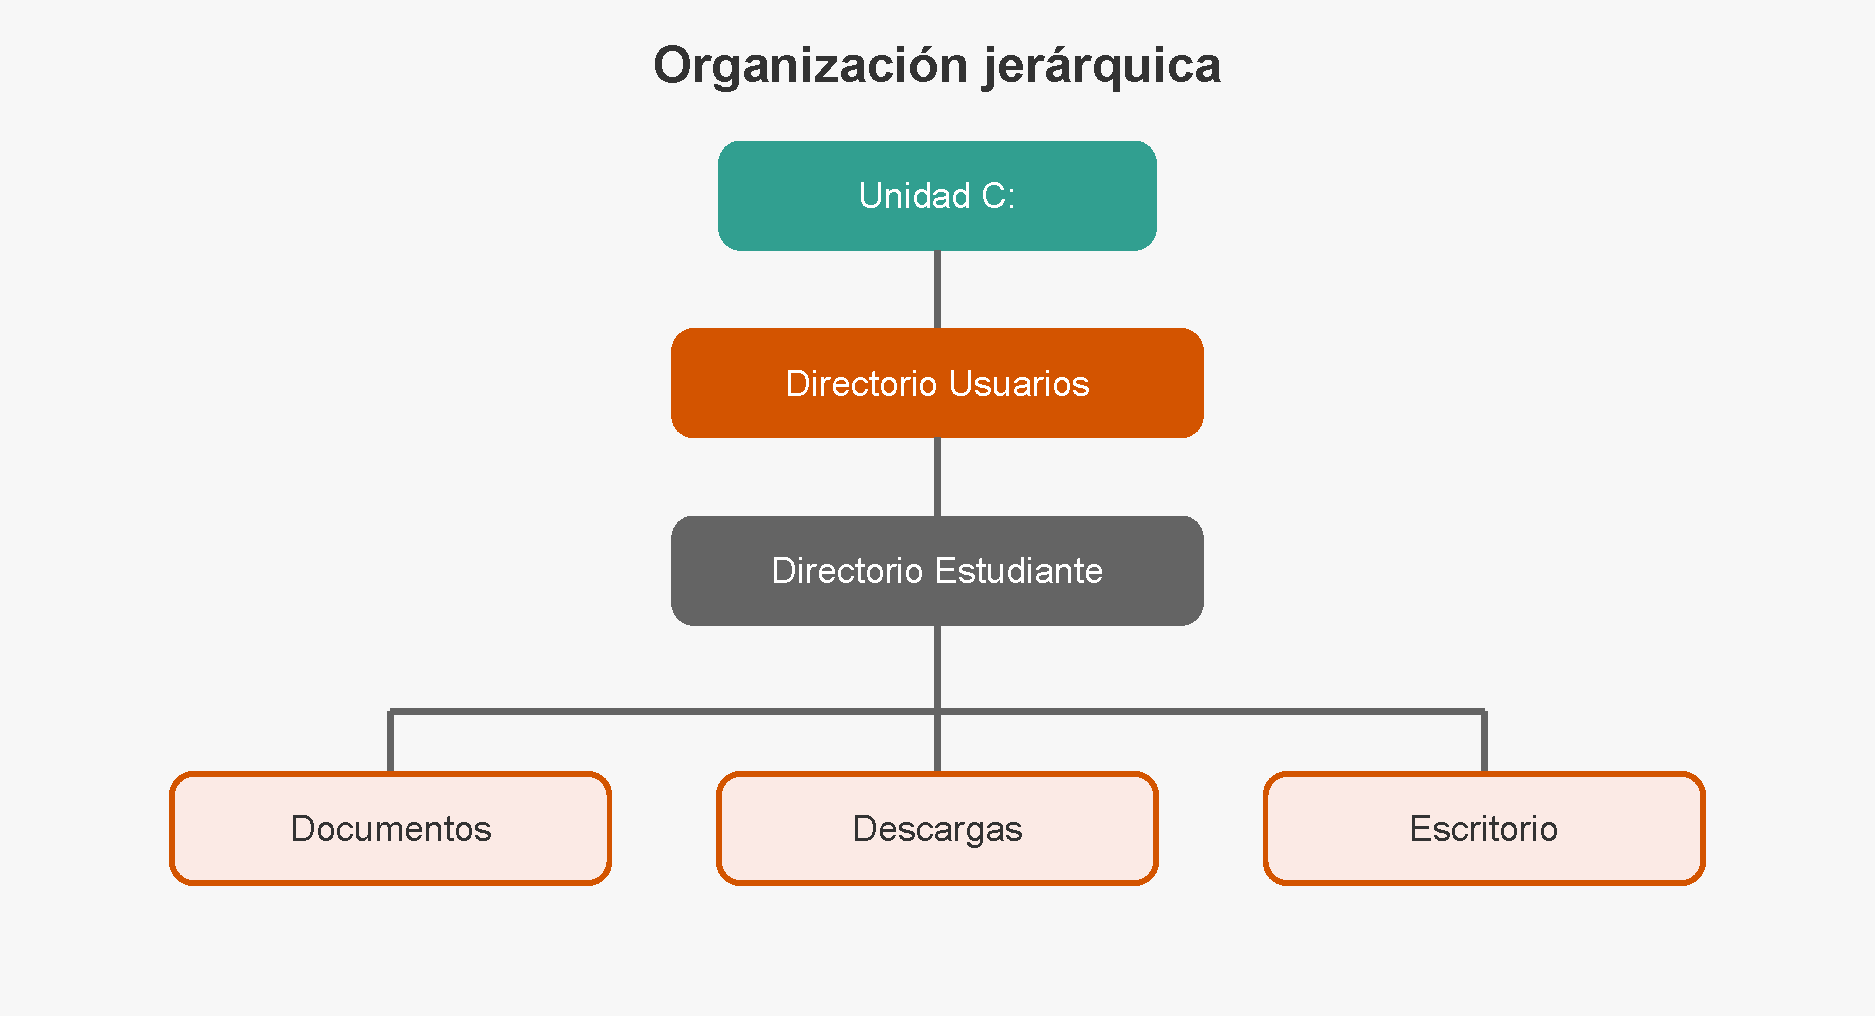
\includegraphics[width=0.88\linewidth,height=\textheight,keepaspectratio]{index_files/mediabag/capitulos/../img/clase_02/fig_02_01_jerarquia.pdf}

}

\caption{\label{fig-jerarquia}Organización jerárquica del sistema de
archivos}

\end{figure}%

En esta estructura:

\begin{itemize}
\tightlist
\item
  La \textbf{unidad} representa un dispositivo o volumen de
  almacenamiento.
\item
  El \textbf{directorio} agrupa información relacionada.
\item
  El \textbf{subdirectorio} es un directorio ubicado dentro de otro.
\item
  El \textbf{archivo} contiene los datos que utiliza el usuario o una
  aplicación.
\end{itemize}

\begin{tcolorbox}[enhanced jigsaw, arc=.35mm, bottomrule=.15mm, bottomtitle=1mm, breakable, colback=white, colbacktitle=quarto-callout-tip-color!10!white, colframe=quarto-callout-tip-color-frame, coltitle=black, left=2mm, leftrule=.75mm, opacityback=0, opacitybacktitle=0.6, rightrule=.15mm, title=\textcolor{quarto-callout-tip-color}{\faLightbulb}\hspace{0.5em}{Consejo del Ingeniero}, titlerule=0mm, toprule=.15mm, toptitle=1mm]

Un archivo bien nombrado y guardado en una estructura lógica puede
ahorrar más tiempo que cualquier comando avanzado.

\end{tcolorbox}

\bookmarksetup{startatroot}

\chapter{El sistema de archivos}\label{el-sistema-de-archivos}

Un \textbf{sistema de archivos} es el conjunto de reglas y estructuras
que utiliza el sistema operativo para registrar, organizar, localizar y
proteger la información dentro de un dispositivo de almacenamiento.

El usuario observa carpetas y nombres. Internamente, el sistema
operativo también mantiene datos como:

\begin{itemize}
\tightlist
\item
  ubicación lógica;
\item
  tamaño;
\item
  fecha de creación y modificación;
\item
  permisos;
\item
  atributos;
\item
  relación entre directorios y archivos.
\end{itemize}

La organización lógica evita que el usuario deba conocer el lugar físico
exacto donde se encuentran los datos dentro del dispositivo.

\section{Unidades de almacenamiento}\label{unidades-de-almacenamiento}

En Windows, las unidades suelen identificarse mediante una letra seguida
de dos puntos:

\begin{Shaded}
\begin{Highlighting}[]
\NormalTok{C:}
\NormalTok{D:}
\NormalTok{E:}
\end{Highlighting}
\end{Shaded}

La unidad \texttt{C:} suele contener el sistema operativo y los perfiles
de usuario. Otras letras pueden representar particiones, memorias USB,
discos externos, unidades ópticas o recursos conectados.

\begin{tcolorbox}[enhanced jigsaw, arc=.35mm, bottomrule=.15mm, bottomtitle=1mm, breakable, colback=white, colbacktitle=quarto-callout-warning-color!10!white, colframe=quarto-callout-warning-color-frame, coltitle=black, left=2mm, leftrule=.75mm, opacityback=0, opacitybacktitle=0.6, rightrule=.15mm, title=\textcolor{quarto-callout-warning-color}{\faExclamationTriangle}\hspace{0.5em}{No confundir}, titlerule=0mm, toprule=.15mm, toptitle=1mm]

La letra no indica por sí sola el tipo de dispositivo. Una memoria USB
puede aparecer como \texttt{D:}, \texttt{E:} o cualquier otra letra
disponible.

\end{tcolorbox}

\section{Directorios y carpetas}\label{directorios-y-carpetas}

En Windows se utiliza con frecuencia la palabra \textbf{carpeta}. En el
lenguaje técnico y en la línea de comandos se emplea el término
\textbf{directorio}.

Ambos describen una estructura que permite agrupar archivos y otros
directorios.

\begin{Shaded}
\begin{Highlighting}[]
\NormalTok{C:\textbackslash{}}
\NormalTok{└── Usuarios}
\NormalTok{    └── Estudiante}
\NormalTok{        ├── Documentos}
\NormalTok{        ├── Descargas}
\NormalTok{        └── Escritorio}
\end{Highlighting}
\end{Shaded}

\section{Archivos y extensiones}\label{archivos-y-extensiones}

Un archivo es una unidad de información identificada mediante un nombre.

\begin{Shaded}
\begin{Highlighting}[]
\NormalTok{informe.docx}
\NormalTok{presupuesto.xlsx}
\NormalTok{programa.cpp}
\NormalTok{manual.pdf}
\NormalTok{imagen.png}
\end{Highlighting}
\end{Shaded}

La parte ubicada después del último punto se denomina
\textbf{extensión}. Esta ayuda al sistema operativo y a las aplicaciones
a reconocer el formato del archivo.

\begin{tcolorbox}[enhanced jigsaw, arc=.35mm, bottomrule=.15mm, bottomtitle=1mm, breakable, colback=white, colbacktitle=quarto-callout-important-color!10!white, colframe=quarto-callout-important-color-frame, coltitle=black, left=2mm, leftrule=.75mm, opacityback=0, opacitybacktitle=0.6, rightrule=.15mm, title=\textcolor{quarto-callout-important-color}{\faExclamation}\hspace{0.5em}{Idea clave}, titlerule=0mm, toprule=.15mm, toptitle=1mm]

Cambiar \texttt{fotografia.jpg} por \texttt{fotografia.pdf} no
transforma la imagen en un PDF. Solo modifica el nombre.

\end{tcolorbox}

\bookmarksetup{startatroot}

\chapter{Rutas: la dirección de la
información}\label{rutas-la-direcciuxf3n-de-la-informaciuxf3n}

Una \textbf{ruta} indica la ubicación de un archivo o directorio dentro
de la jerarquía del sistema.

\begin{figure}

\centering{

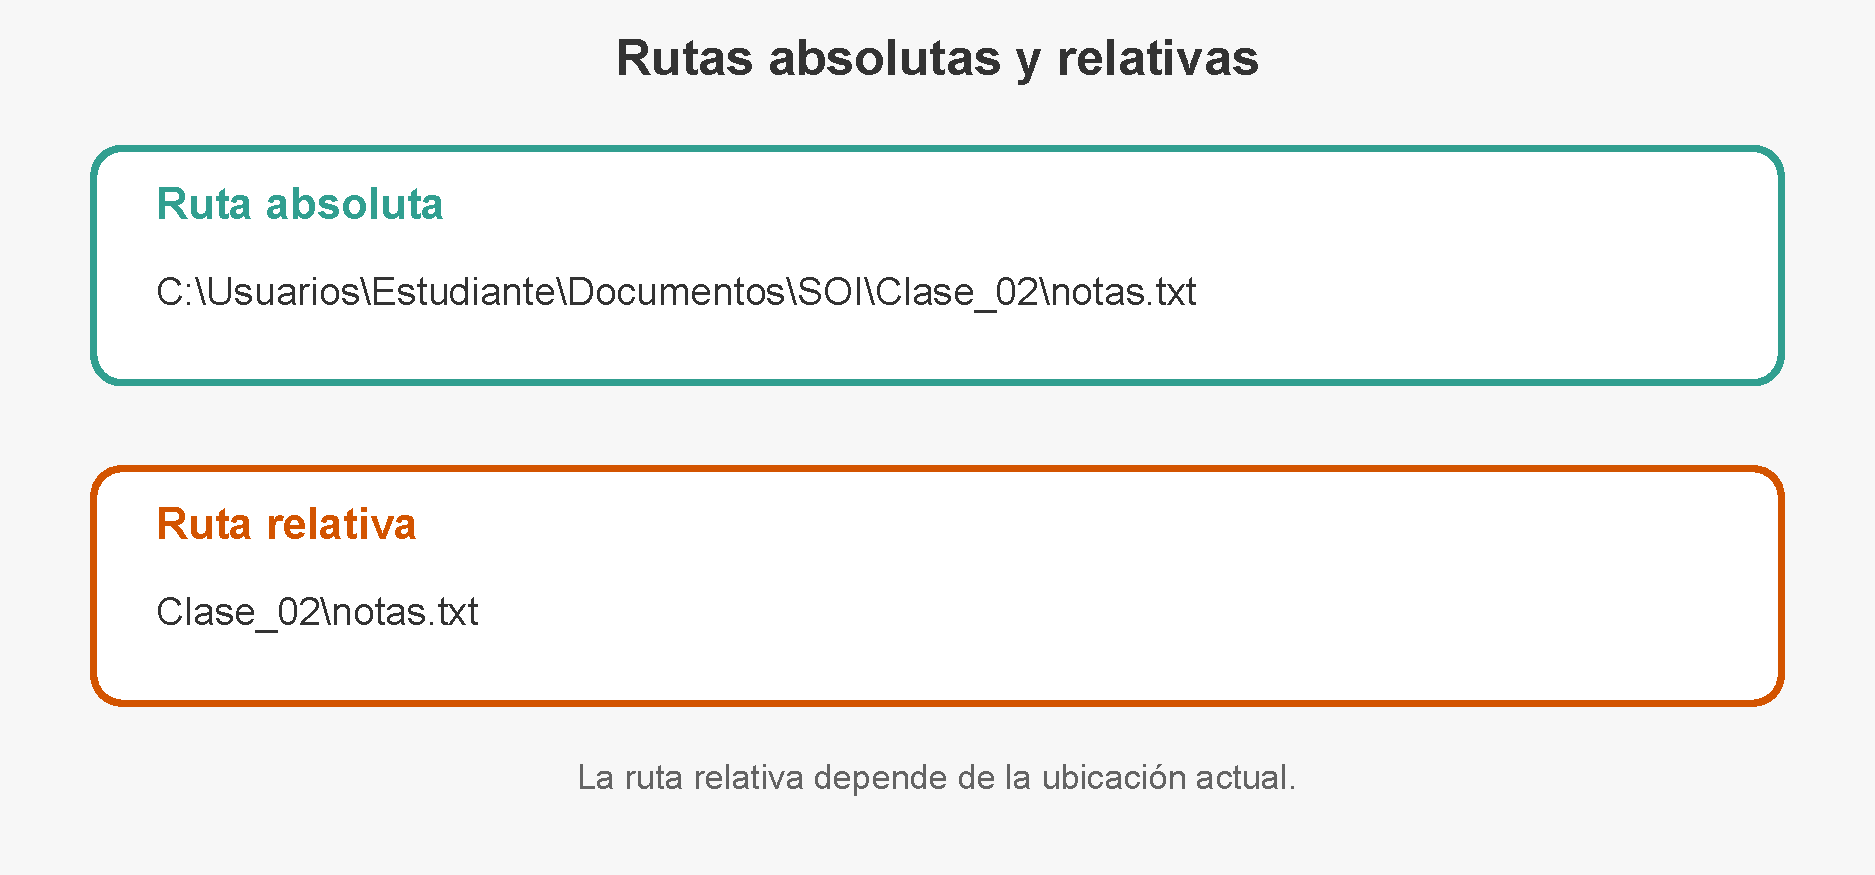
\includegraphics[width=0.92\linewidth,height=\textheight,keepaspectratio]{index_files/mediabag/capitulos/../img/clase_02/fig_02_02_rutas.pdf}

}

\caption{\label{fig-rutas}Ruta absoluta y ruta relativa}

\end{figure}%

\section{Ruta absoluta}\label{ruta-absoluta}

Una ruta absoluta comienza desde la unidad y describe el recorrido
completo.

\begin{Shaded}
\begin{Highlighting}[]
\NormalTok{C:\textbackslash{}Usuarios\textbackslash{}Estudiante\textbackslash{}Documentos\textbackslash{}SOI\textbackslash{}Clase\_02\textbackslash{}notas.txt}
\end{Highlighting}
\end{Shaded}

Esta ruta puede interpretarse de izquierda a derecha:

\begin{enumerate}
\def\labelenumi{\arabic{enumi}.}
\tightlist
\item
  Unidad \texttt{C:}.
\item
  Directorio \texttt{Usuarios}.
\item
  Perfil \texttt{Estudiante}.
\item
  Directorio \texttt{Documentos}.
\item
  Proyecto \texttt{SOI}.
\item
  Directorio \texttt{Clase\_02}.
\item
  Archivo \texttt{notas.txt}.
\end{enumerate}

\section{Ruta relativa}\label{ruta-relativa}

Una ruta relativa se interpreta desde la ubicación actual.

Si la ubicación actual es:

\begin{Shaded}
\begin{Highlighting}[]
\NormalTok{C:\textbackslash{}Usuarios\textbackslash{}Estudiante\textbackslash{}Documentos\textbackslash{}SOI}
\end{Highlighting}
\end{Shaded}

la ruta relativa hacia el archivo anterior sería:

\begin{Shaded}
\begin{Highlighting}[]
\NormalTok{Clase\_02\textbackslash{}notas.txt}
\end{Highlighting}
\end{Shaded}

El símbolo \texttt{..} representa el directorio superior.

\begin{Shaded}
\begin{Highlighting}[]
\NormalTok{cd ..}
\end{Highlighting}
\end{Shaded}

significa:

\begin{quote}
Subir un nivel dentro de la estructura.
\end{quote}

\section{Separadores y espacios}\label{separadores-y-espacios}

Windows utiliza la barra invertida \texttt{\textbackslash{}} para
separar los componentes de una ruta.

Cuando una ruta contiene espacios, es recomendable escribirla entre
comillas:

\begin{Shaded}
\begin{Highlighting}[]
\NormalTok{cd "C:\textbackslash{}Usuarios\textbackslash{}Estudiante\textbackslash{}Mis documentos"}
\end{Highlighting}
\end{Shaded}

\bookmarksetup{startatroot}

\chapter{De la interfaz gráfica a la línea de
comandos}\label{de-la-interfaz-gruxe1fica-a-la-luxednea-de-comandos}

La interfaz gráfica permite administrar información mediante ventanas,
iconos, menús y el puntero. La interfaz de línea de comandos permite
hacerlo escribiendo instrucciones.

{\def\LTcaptype{none} % do not increment counter
\begin{longtable}[]{@{}ll@{}}
\toprule\noalign{}
Interfaz gráfica & Línea de comandos \\
\midrule\noalign{}
\endhead
\bottomrule\noalign{}
\endlastfoot
Utiliza ventanas e iconos & Utiliza instrucciones escritas \\
Es visual e intuitiva & Es precisa y reproducible \\
Facilita tareas ocasionales & Facilita automatización y diagnóstico \\
Requiere navegación manual & Puede ejecutar secuencias rápidamente \\
\end{longtable}
}

Ninguna reemplaza completamente a la otra. Un profesional utiliza la
herramienta más adecuada para cada situación.

\bookmarksetup{startatroot}

\chapter{¿Qué es un comando?}\label{quuxe9-es-un-comando}

Un \textbf{comando} es una instrucción que el usuario entrega a un
intérprete para solicitar una acción.

Ejemplos:

\begin{Shaded}
\begin{Highlighting}[]
\BuiltInTok{dir}
\end{Highlighting}
\end{Shaded}

Solicita mostrar el contenido del directorio actual.

\begin{Shaded}
\begin{Highlighting}[]
\BuiltInTok{mkdir}\NormalTok{ Clase\_02}
\end{Highlighting}
\end{Shaded}

Solicita crear un directorio llamado \texttt{Clase\_02}.

\begin{Shaded}
\begin{Highlighting}[]
\BuiltInTok{copy}\NormalTok{ notas.txt respaldo.txt}
\end{Highlighting}
\end{Shaded}

Solicita crear una copia del archivo.

Los comandos pueden aceptar:

\begin{itemize}
\tightlist
\item
  \textbf{argumentos}, que indican sobre qué elemento trabajar;
\item
  \textbf{opciones}, que modifican la forma en que se ejecuta la
  instrucción.
\end{itemize}

Ejemplo:

\begin{Shaded}
\begin{Highlighting}[]
\BuiltInTok{dir} \AttributeTok{/w}
\end{Highlighting}
\end{Shaded}

\begin{itemize}
\tightlist
\item
  \texttt{dir} es el comando.
\item
  \texttt{/w} es una opción que muestra una vista resumida.
\end{itemize}

\bookmarksetup{startatroot}

\chapter{CMD en Windows}\label{cmd-en-windows}

El \textbf{Símbolo del sistema}, también conocido como \textbf{CMD}, es
un intérprete de comandos incluido en Windows.

No debe confundirse con MS-DOS. Aunque conserva numerosos comandos
históricos, CMD funciona dentro de Windows y utiliza los servicios del
sistema operativo actual.

\section{Cómo abrirlo}\label{cuxf3mo-abrirlo}

Puede abrirse de distintas maneras:

\begin{enumerate}
\def\labelenumi{\arabic{enumi}.}
\tightlist
\item
  Presionar la tecla Windows.
\item
  Escribir \texttt{cmd}.
\item
  Seleccionar \textbf{Símbolo del sistema}.
\end{enumerate}

También puede utilizarse la ventana \textbf{Ejecutar}:

\begin{Shaded}
\begin{Highlighting}[]
\NormalTok{Windows + R}
\end{Highlighting}
\end{Shaded}

Luego escribir:

\begin{Shaded}
\begin{Highlighting}[]
\NormalTok{cmd}
\end{Highlighting}
\end{Shaded}

y presionar Enter.

\begin{tcolorbox}[enhanced jigsaw, arc=.35mm, bottomrule=.15mm, bottomtitle=1mm, breakable, colback=white, colbacktitle=quarto-callout-warning-color!10!white, colframe=quarto-callout-warning-color-frame, coltitle=black, left=2mm, leftrule=.75mm, opacityback=0, opacitybacktitle=0.6, rightrule=.15mm, title=\textcolor{quarto-callout-warning-color}{\faExclamationTriangle}\hspace{0.5em}{Permisos administrativos}, titlerule=0mm, toprule=.15mm, toptitle=1mm]

Para esta práctica no es necesario abrir CMD como administrador.
Trabajar con privilegios elevados aumenta el impacto de un error.

\end{tcolorbox}

\bookmarksetup{startatroot}

\chapter{Anatomía del prompt}\label{anatomuxeda-del-prompt}

Al abrir CMD aparece una línea similar a:

\begin{Shaded}
\begin{Highlighting}[]
\NormalTok{C:\textbackslash{}Users\textbackslash{}Estudiante\textgreater{}}
\end{Highlighting}
\end{Shaded}

\begin{figure}

\centering{

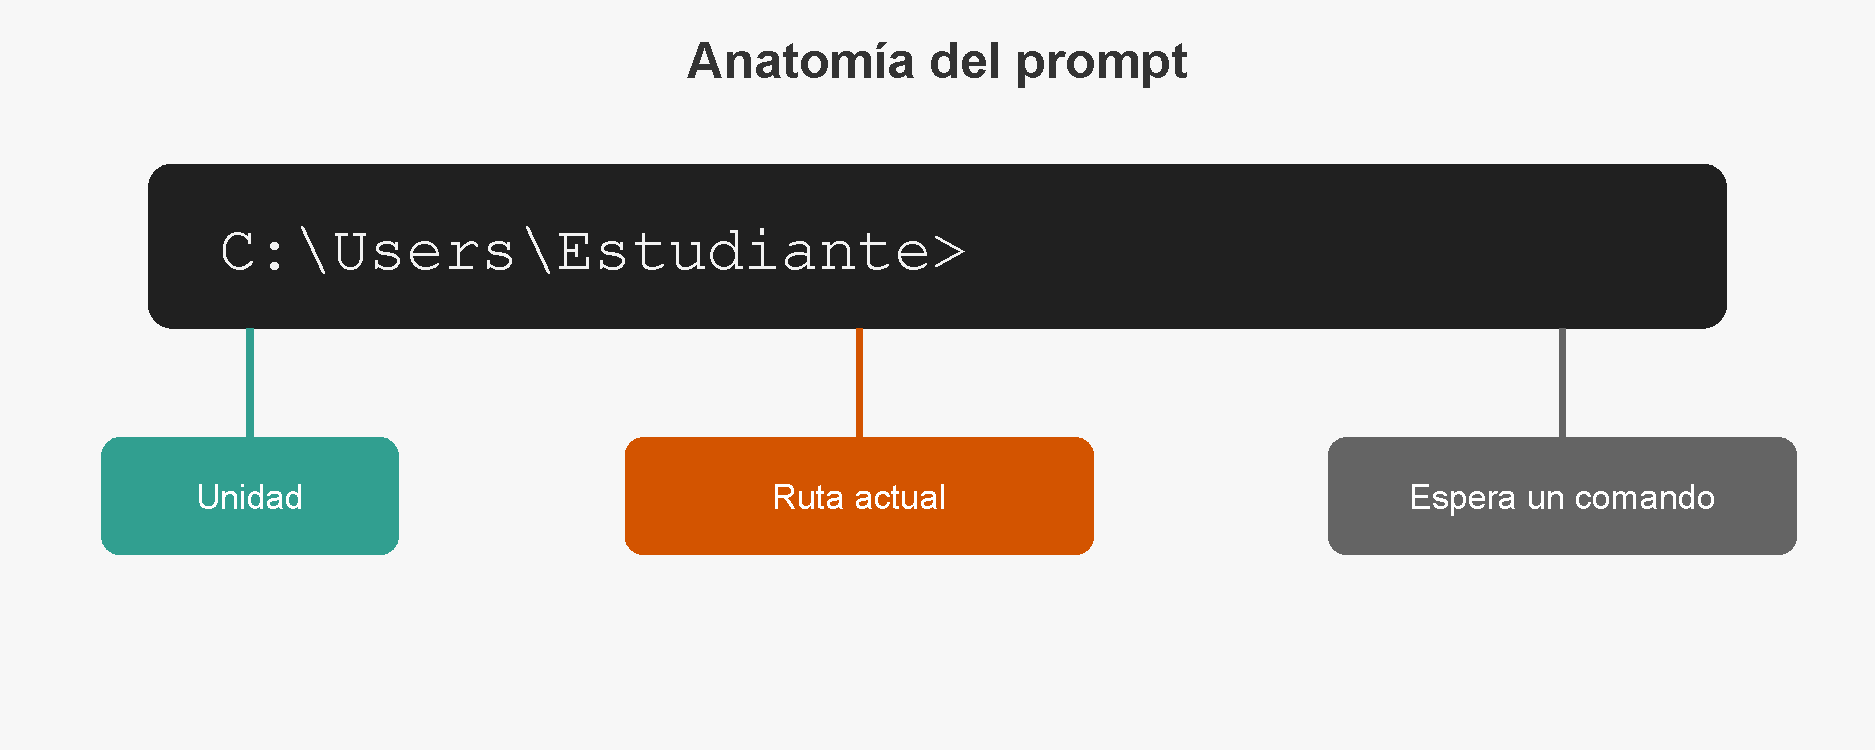
\includegraphics[width=0.88\linewidth,height=\textheight,keepaspectratio]{index_files/mediabag/capitulos/../img/clase_02/fig_02_03_prompt.pdf}

}

\caption{\label{fig-prompt}Anatomía del prompt de CMD}

\end{figure}%

El prompt muestra la ubicación actual y termina con el símbolo
\texttt{\textgreater{}} para indicar que el intérprete espera una
instrucción.

\begin{Shaded}
\begin{Highlighting}[]
\NormalTok{C:                         unidad}
\NormalTok{\textbackslash{}Users\textbackslash{}Estudiante          ruta actual}
\NormalTok{\textgreater{}                          espera un comando}
\end{Highlighting}
\end{Shaded}

\begin{tcolorbox}[enhanced jigsaw, arc=.35mm, bottomrule=.15mm, bottomtitle=1mm, breakable, colback=white, colbacktitle=quarto-callout-note-color!10!white, colframe=quarto-callout-note-color-frame, coltitle=black, left=2mm, leftrule=.75mm, opacityback=0, opacitybacktitle=0.6, rightrule=.15mm, title=\textcolor{quarto-callout-note-color}{\faInfo}\hspace{0.5em}{Observe}, titlerule=0mm, toprule=.15mm, toptitle=1mm]

Cada vez que cambia de directorio, el prompt también cambia. Por eso
funciona como una brújula dentro del sistema de archivos.

\end{tcolorbox}

\bookmarksetup{startatroot}

\chapter{Laboratorio narrativo: construyendo el proyecto
SOI}\label{laboratorio-narrativo-construyendo-el-proyecto-soi}

\section{Situación}\label{situaciuxf3n}

Durante el semestre se generarán apuntes, prácticas, recursos y
entregables. Para evitar que todo quede mezclado, construiremos una
estructura permanente llamada \texttt{SOI}.

El laboratorio se realizará dentro de \textbf{Documentos}. No trabaje en
directorios del sistema como \texttt{C:\textbackslash{}Windows} o
\texttt{C:\textbackslash{}Program\ Files}.

\section{Paso 1. Saber dónde
estamos}\label{paso-1.-saber-duxf3nde-estamos}

Escriba:

\begin{Shaded}
\begin{Highlighting}[]
\BuiltInTok{cd}
\end{Highlighting}
\end{Shaded}

CMD mostrará la ruta actual.

También puede observarla directamente en el prompt.

\section{Paso 2. Ver el contenido}\label{paso-2.-ver-el-contenido}

Ejecute:

\begin{Shaded}
\begin{Highlighting}[]
\BuiltInTok{dir}
\end{Highlighting}
\end{Shaded}

El comando \texttt{dir} muestra directorios y archivos de la ubicación
actual.

En la salida encontrará datos como:

\begin{itemize}
\tightlist
\item
  fecha y hora;
\item
  indicador \texttt{\textless{}DIR\textgreater{}} para directorios;
\item
  tamaño de archivos;
\item
  nombre de cada elemento.
\end{itemize}

\subsection{Variantes útiles}\label{variantes-uxfatiles}

\begin{Shaded}
\begin{Highlighting}[]
\BuiltInTok{dir} \AttributeTok{/w}
\end{Highlighting}
\end{Shaded}

Muestra una vista resumida.

\begin{Shaded}
\begin{Highlighting}[]
\BuiltInTok{dir} \AttributeTok{/p}
\end{Highlighting}
\end{Shaded}

Pausa la salida cuando ocupa más de una pantalla.

\begin{Shaded}
\begin{Highlighting}[]
\BuiltInTok{dir}\NormalTok{ *.txt}
\end{Highlighting}
\end{Shaded}

Muestra únicamente archivos con extensión \texttt{.txt}.

\begin{tcolorbox}[enhanced jigsaw, arc=.35mm, bottomrule=.15mm, bottomtitle=1mm, breakable, colback=white, colbacktitle=quarto-callout-tip-color!10!white, colframe=quarto-callout-tip-color-frame, coltitle=black, left=2mm, leftrule=.75mm, opacityback=0, opacitybacktitle=0.6, rightrule=.15mm, title=\textcolor{quarto-callout-tip-color}{\faLightbulb}\hspace{0.5em}{Lectura antes de acción}, titlerule=0mm, toprule=.15mm, toptitle=1mm]

Antes de crear, mover o borrar algo, use \texttt{dir}. Confirmar la
ubicación reduce errores.

\end{tcolorbox}

\section{Paso 3. Ir a Documentos}\label{paso-3.-ir-a-documentos}

Según el idioma y la configuración de Windows, el nombre visible puede
variar. Una forma práctica es utilizar la variable del perfil:

\begin{Shaded}
\begin{Highlighting}[]
\BuiltInTok{cd} \AttributeTok{/d} \StringTok{"}\PreprocessorTok{\%}\VariableTok{USERPROFILE}\PreprocessorTok{\%}\StringTok{\textbackslash{}Documents"}
\end{Highlighting}
\end{Shaded}

Si la carpeta se muestra en español pero la ruta interna utiliza
\texttt{Documents}, el comando seguirá funcionando.

La opción \texttt{/d} permite cambiar de unidad y directorio en una sola
instrucción.

\section{Paso 4. Crear el directorio
principal}\label{paso-4.-crear-el-directorio-principal}

\begin{Shaded}
\begin{Highlighting}[]
\BuiltInTok{mkdir}\NormalTok{ SOI}
\end{Highlighting}
\end{Shaded}

También puede utilizarse la forma abreviada:

\begin{Shaded}
\begin{Highlighting}[]
\BuiltInTok{md}\NormalTok{ SOI}
\end{Highlighting}
\end{Shaded}

Ambos comandos crean el directorio.

Compruebe el resultado:

\begin{Shaded}
\begin{Highlighting}[]
\BuiltInTok{dir}
\end{Highlighting}
\end{Shaded}

\section{Paso 5. Entrar al proyecto}\label{paso-5.-entrar-al-proyecto}

\begin{Shaded}
\begin{Highlighting}[]
\BuiltInTok{cd}\NormalTok{ SOI}
\end{Highlighting}
\end{Shaded}

El prompt debería terminar de forma similar a:

\begin{Shaded}
\begin{Highlighting}[]
\NormalTok{...\textbackslash{}Documents\textbackslash{}SOI\textgreater{}}
\end{Highlighting}
\end{Shaded}

\section{Paso 6. Crear la estructura del
semestre}\label{paso-6.-crear-la-estructura-del-semestre}

Ejecute:

\begin{Shaded}
\begin{Highlighting}[]
\BuiltInTok{mkdir}\NormalTok{ Clase\_01 Clase\_02 Clase\_03 Laboratorios Recursos Proyecto\_Final}
\end{Highlighting}
\end{Shaded}

Luego verifique:

\begin{Shaded}
\begin{Highlighting}[]
\BuiltInTok{dir}
\end{Highlighting}
\end{Shaded}

La estructura esperada es:

\begin{Shaded}
\begin{Highlighting}[]
\NormalTok{SOI}
\NormalTok{├── Clase\_01}
\NormalTok{├── Clase\_02}
\NormalTok{├── Clase\_03}
\NormalTok{├── Laboratorios}
\NormalTok{├── Recursos}
\NormalTok{└── Proyecto\_Final}
\end{Highlighting}
\end{Shaded}

\begin{figure}

\centering{

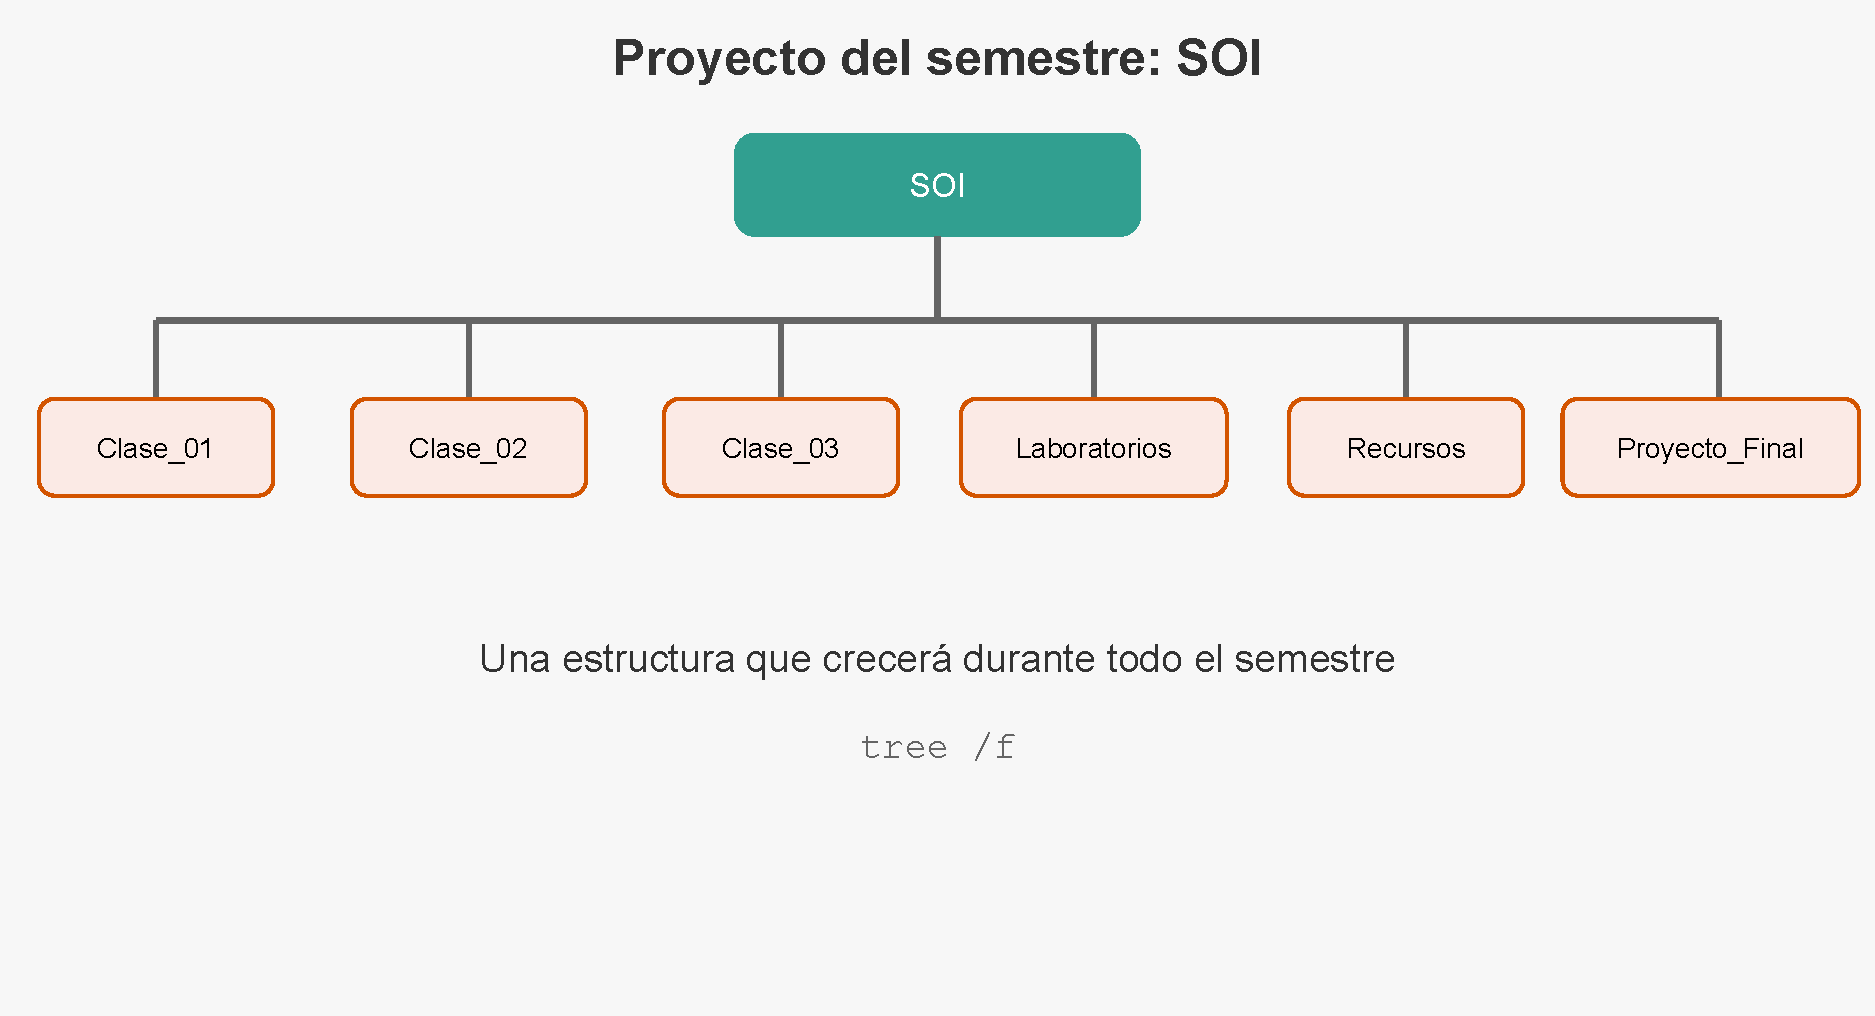
\includegraphics[width=0.84\linewidth,height=\textheight,keepaspectratio]{index_files/mediabag/capitulos/../img/clase_02/fig_02_04_proyecto_soi.pdf}

}

\caption{\label{fig-proyecto}Estructura inicial del proyecto SOI}

\end{figure}%

\section{Paso 7. Visualizar el
árbol}\label{paso-7.-visualizar-el-uxe1rbol}

Ejecute:

\begin{Shaded}
\begin{Highlighting}[]
\KeywordTok{tree}
\end{Highlighting}
\end{Shaded}

Para incluir también archivos:

\begin{Shaded}
\begin{Highlighting}[]
\KeywordTok{tree} \AttributeTok{/f}
\end{Highlighting}
\end{Shaded}

\texttt{tree} permite comprobar visualmente la jerarquía construida.

\bookmarksetup{startatroot}

\chapter{\texorpdfstring{Navegación con
\texttt{cd}}{Navegación con cd}}\label{navegaciuxf3n-con-cd}

El comando \texttt{cd} significa \textbf{change directory}, es decir,
cambiar de directorio.

\section{Entrar a un directorio}\label{entrar-a-un-directorio}

\begin{Shaded}
\begin{Highlighting}[]
\BuiltInTok{cd}\NormalTok{ Clase\_02}
\end{Highlighting}
\end{Shaded}

\section{Subir un nivel}\label{subir-un-nivel}

\begin{Shaded}
\begin{Highlighting}[]
\BuiltInTok{cd}\NormalTok{ ..}
\end{Highlighting}
\end{Shaded}

\section{Ir a la raíz de la unidad}\label{ir-a-la-rauxedz-de-la-unidad}

\begin{Shaded}
\begin{Highlighting}[]
\BuiltInTok{cd} \SpecialCharTok{\textbackslash{}}
\end{Highlighting}
\end{Shaded}

\section{Cambiar directamente mediante una
ruta}\label{cambiar-directamente-mediante-una-ruta}

\begin{Shaded}
\begin{Highlighting}[]
\BuiltInTok{cd} \AttributeTok{/d} \StringTok{"}\PreprocessorTok{\%}\VariableTok{USERPROFILE}\PreprocessorTok{\%}\StringTok{\textbackslash{}Documents\textbackslash{}SOI\textbackslash{}Clase\_02"}
\end{Highlighting}
\end{Shaded}

\section{Volver al directorio
anterior}\label{volver-al-directorio-anterior}

CMD no ofrece exactamente el mismo comportamiento que algunos
intérpretes modernos, por lo que conviene leer el prompt y utilizar
rutas relativas o absolutas de manera consciente.

\begin{tcolorbox}[enhanced jigsaw, arc=.35mm, bottomrule=.15mm, bottomtitle=1mm, breakable, colback=white, colbacktitle=quarto-callout-warning-color!10!white, colframe=quarto-callout-warning-color-frame, coltitle=black, left=2mm, leftrule=.75mm, opacityback=0, opacitybacktitle=0.6, rightrule=.15mm, title=\textcolor{quarto-callout-warning-color}{\faExclamationTriangle}\hspace{0.5em}{Error común}, titlerule=0mm, toprule=.15mm, toptitle=1mm]

\texttt{cd...} no es la forma correcta de subir un nivel. Debe existir
un espacio:

\begin{Shaded}
\begin{Highlighting}[]
\BuiltInTok{cd}\NormalTok{ ..}
\end{Highlighting}
\end{Shaded}

\end{tcolorbox}

\bookmarksetup{startatroot}

\chapter{Crear archivos de
práctica}\label{crear-archivos-de-pruxe1ctica}

Para continuar necesitamos archivos sencillos.

Ubíquese dentro de \texttt{Clase\_02}:

\begin{Shaded}
\begin{Highlighting}[]
\BuiltInTok{cd} \AttributeTok{/d} \StringTok{"}\PreprocessorTok{\%}\VariableTok{USERPROFILE}\PreprocessorTok{\%}\StringTok{\textbackslash{}Documents\textbackslash{}SOI\textbackslash{}Clase\_02"}
\end{Highlighting}
\end{Shaded}

Cree un archivo de texto:

\begin{Shaded}
\begin{Highlighting}[]
\BuiltInTok{echo}\NormalTok{ Apuntes de la Clase 2 }\KeywordTok{\textgreater{}}\NormalTok{ apuntes.txt}
\end{Highlighting}
\end{Shaded}

Agregue una segunda línea:

\begin{Shaded}
\begin{Highlighting}[]
\BuiltInTok{echo}\NormalTok{ Practica de comandos de Windows }\KeywordTok{\textgreater{}\textgreater{}}\NormalTok{ apuntes.txt}
\end{Highlighting}
\end{Shaded}

Los operadores utilizados son:

\begin{itemize}
\tightlist
\item
  \texttt{\textgreater{}} crea o reemplaza el contenido.
\item
  \texttt{\textgreater{}\textgreater{}} agrega contenido al final.
\end{itemize}

Compruebe el archivo:

\begin{Shaded}
\begin{Highlighting}[]
\BuiltInTok{dir}
\end{Highlighting}
\end{Shaded}

Muestre su contenido:

\begin{Shaded}
\begin{Highlighting}[]
\BuiltInTok{type}\NormalTok{ apuntes.txt}
\end{Highlighting}
\end{Shaded}

\begin{tcolorbox}[enhanced jigsaw, arc=.35mm, bottomrule=.15mm, bottomtitle=1mm, breakable, colback=white, colbacktitle=quarto-callout-important-color!10!white, colframe=quarto-callout-important-color-frame, coltitle=black, left=2mm, leftrule=.75mm, opacityback=0, opacitybacktitle=0.6, rightrule=.15mm, title=\textcolor{quarto-callout-important-color}{\faExclamation}\hspace{0.5em}{Precaución}, titlerule=0mm, toprule=.15mm, toptitle=1mm]

El operador \texttt{\textgreater{}} reemplaza el contenido existente.
Antes de usarlo sobre un archivo importante, compruebe el nombre y la
ruta.

\end{tcolorbox}

\bookmarksetup{startatroot}

\chapter{\texorpdfstring{Copiar archivos con
\texttt{copy}}{Copiar archivos con copy}}\label{copiar-archivos-con-copy}

El comando \texttt{copy} crea una copia de uno o varios archivos.

\section{Copiar en el mismo
directorio}\label{copiar-en-el-mismo-directorio}

\begin{Shaded}
\begin{Highlighting}[]
\BuiltInTok{copy}\NormalTok{ apuntes.txt respaldo\_apuntes.txt}
\end{Highlighting}
\end{Shaded}

\section{Copiar hacia otro
directorio}\label{copiar-hacia-otro-directorio}

\begin{Shaded}
\begin{Highlighting}[]
\BuiltInTok{copy}\NormalTok{ apuntes.txt ..\textbackslash{}Recursos\textbackslash{}}
\end{Highlighting}
\end{Shaded}

La ruta \texttt{..\textbackslash{}Recursos\textbackslash{}} significa:

\begin{enumerate}
\def\labelenumi{\arabic{enumi}.}
\tightlist
\item
  subir desde \texttt{Clase\_02} hacia \texttt{SOI};
\item
  entrar en \texttt{Recursos}.
\end{enumerate}

Compruebe el resultado:

\begin{Shaded}
\begin{Highlighting}[]
\BuiltInTok{dir}\NormalTok{ ..\textbackslash{}Recursos}
\end{Highlighting}
\end{Shaded}

\section{Evitar sobrescrituras
accidentales}\label{evitar-sobrescrituras-accidentales}

Puede utilizar:

\begin{Shaded}
\begin{Highlighting}[]
\BuiltInTok{copy}\NormalTok{ /}\AttributeTok{{-}y}\NormalTok{ apuntes.txt respaldo\_apuntes.txt}
\end{Highlighting}
\end{Shaded}

La opción \texttt{/-y} solicita confirmación antes de reemplazar un
archivo existente.

\bookmarksetup{startatroot}

\chapter{\texorpdfstring{Renombrar con
\texttt{ren}}{Renombrar con ren}}\label{renombrar-con-ren}

El comando \texttt{ren} cambia el nombre de un archivo o directorio.

\begin{Shaded}
\begin{Highlighting}[]
\BuiltInTok{ren}\NormalTok{ respaldo\_apuntes.txt apuntes\_copia.txt}
\end{Highlighting}
\end{Shaded}

Compruebe:

\begin{Shaded}
\begin{Highlighting}[]
\BuiltInTok{dir}
\end{Highlighting}
\end{Shaded}

La instrucción cambia el nombre, pero no traslada el archivo a otra
ubicación.

\begin{tcolorbox}[enhanced jigsaw, arc=.35mm, bottomrule=.15mm, bottomtitle=1mm, breakable, colback=white, colbacktitle=quarto-callout-note-color!10!white, colframe=quarto-callout-note-color-frame, coltitle=black, left=2mm, leftrule=.75mm, opacityback=0, opacitybacktitle=0.6, rightrule=.15mm, title=\textcolor{quarto-callout-note-color}{\faInfo}\hspace{0.5em}{Diferencia importante}, titlerule=0mm, toprule=.15mm, toptitle=1mm]

\begin{itemize}
\tightlist
\item
  \texttt{ren} cambia el nombre.
\item
  \texttt{move} cambia la ubicación y también puede cambiar el nombre.
\end{itemize}

\end{tcolorbox}

\bookmarksetup{startatroot}

\chapter{\texorpdfstring{Mover con
\texttt{move}}{Mover con move}}\label{mover-con-move}

Para trasladar un archivo:

\begin{Shaded}
\begin{Highlighting}[]
\BuiltInTok{move}\NormalTok{ apuntes\_copia.txt ..\textbackslash{}Laboratorios\textbackslash{}}
\end{Highlighting}
\end{Shaded}

Compruebe el directorio de destino:

\begin{Shaded}
\begin{Highlighting}[]
\BuiltInTok{dir}\NormalTok{ ..\textbackslash{}Laboratorios}
\end{Highlighting}
\end{Shaded}

También puede mover y renombrar en una sola instrucción:

\begin{Shaded}
\begin{Highlighting}[]
\BuiltInTok{move}\NormalTok{ apuntes.txt ..\textbackslash{}Laboratorios\textbackslash{}bitacora\_clase\_02.txt}
\end{Highlighting}
\end{Shaded}

\bookmarksetup{startatroot}

\chapter{\texorpdfstring{Eliminar archivos con
\texttt{del}}{Eliminar archivos con del}}\label{eliminar-archivos-con-del}

El comando \texttt{del} elimina archivos.

Primero cree un archivo temporal:

\begin{Shaded}
\begin{Highlighting}[]
\BuiltInTok{echo}\NormalTok{ Archivo temporal }\KeywordTok{\textgreater{}}\NormalTok{ temporal.txt}
\end{Highlighting}
\end{Shaded}

Compruebe:

\begin{Shaded}
\begin{Highlighting}[]
\BuiltInTok{dir}
\end{Highlighting}
\end{Shaded}

Luego elimínelo solicitando confirmación:

\begin{Shaded}
\begin{Highlighting}[]
\BuiltInTok{del} \AttributeTok{/p}\NormalTok{ temporal.txt}
\end{Highlighting}
\end{Shaded}

\begin{tcolorbox}[enhanced jigsaw, arc=.35mm, bottomrule=.15mm, bottomtitle=1mm, breakable, colback=white, colbacktitle=quarto-callout-warning-color!10!white, colframe=quarto-callout-warning-color-frame, coltitle=black, left=2mm, leftrule=.75mm, opacityback=0, opacitybacktitle=0.6, rightrule=.15mm, title=\textcolor{quarto-callout-warning-color}{\faExclamationTriangle}\hspace{0.5em}{Advertencia}, titlerule=0mm, toprule=.15mm, toptitle=1mm]

Los archivos eliminados desde CMD normalmente no pasan por la Papelera
de reciclaje. Verifique siempre la ruta, el nombre y los comodines antes
de confirmar.

\end{tcolorbox}

\section{Riesgo de los comodines}\label{riesgo-de-los-comodines}

\begin{Shaded}
\begin{Highlighting}[]
\BuiltInTok{del}\NormalTok{ *.txt}
\end{Highlighting}
\end{Shaded}

elimina todos los archivos \texttt{.txt} del directorio actual.

Este tipo de instrucción no debe ejecutarse sin revisar previamente:

\begin{Shaded}
\begin{Highlighting}[]
\BuiltInTok{dir}\NormalTok{ *.txt}
\end{Highlighting}
\end{Shaded}

La secuencia profesional es:

\begin{Shaded}
\begin{Highlighting}[]
\NormalTok{1. Mostrar}
\NormalTok{2. Verificar}
\NormalTok{3. Ejecutar}
\end{Highlighting}
\end{Shaded}

\bookmarksetup{startatroot}

\chapter{\texorpdfstring{Eliminar directorios con
\texttt{rmdir}}{Eliminar directorios con rmdir}}\label{eliminar-directorios-con-rmdir}

\texttt{rmdir} o \texttt{rd} elimina directorios.

\section{Directorio vacío}\label{directorio-vacuxedo}

\begin{Shaded}
\begin{Highlighting}[]
\BuiltInTok{mkdir}\NormalTok{ Prueba\_Vacia}
\BuiltInTok{rmdir}\NormalTok{ Prueba\_Vacia}
\end{Highlighting}
\end{Shaded}

\section{Directorio con contenido}\label{directorio-con-contenido}

\begin{Shaded}
\begin{Highlighting}[]
\BuiltInTok{rmdir} \AttributeTok{/s}\NormalTok{ Carpeta}
\end{Highlighting}
\end{Shaded}

La opción \texttt{/s} incluye todo su contenido.

Para solicitar confirmación:

\begin{Shaded}
\begin{Highlighting}[]
\BuiltInTok{rmdir} \AttributeTok{/s}\NormalTok{ Carpeta}
\end{Highlighting}
\end{Shaded}

Para omitirla existe \texttt{/q}, pero no debe utilizarse durante el
aprendizaje:

\begin{Shaded}
\begin{Highlighting}[]
\BuiltInTok{rmdir} \AttributeTok{/s} \AttributeTok{/q}\NormalTok{ Carpeta}
\end{Highlighting}
\end{Shaded}

\texttt{rmdir\ /s\ /q} puede eliminar una estructura completa sin
preguntar. No lo utilice fuera de carpetas de práctica.

\bookmarksetup{startatroot}

\chapter{\texorpdfstring{Limpiar la pantalla con
\texttt{cls}}{Limpiar la pantalla con cls}}\label{limpiar-la-pantalla-con-cls}

\begin{Shaded}
\begin{Highlighting}[]
\BuiltInTok{cls}
\end{Highlighting}
\end{Shaded}

Este comando limpia la pantalla, pero no elimina archivos ni modifica la
ubicación actual.

Después de ejecutarlo, el prompt continúa en el mismo directorio.

\bookmarksetup{startatroot}

\chapter{Resumen de comandos}\label{resumen-de-comandos}

{\def\LTcaptype{none} % do not increment counter
\begin{longtable}[]{@{}lll@{}}
\toprule\noalign{}
Necesidad & Comando principal & Ejemplo \\
\midrule\noalign{}
\endhead
\bottomrule\noalign{}
\endlastfoot
Mostrar ubicación & \texttt{cd} & \texttt{cd} \\
Listar contenido & \texttt{dir} & \texttt{dir\ /w} \\
Cambiar directorio & \texttt{cd} & \texttt{cd\ Clase\_02} \\
Crear directorio & \texttt{mkdir} o \texttt{md} &
\texttt{mkdir\ Recursos} \\
Mostrar árbol & \texttt{tree} & \texttt{tree\ /f} \\
Mostrar texto & \texttt{type} & \texttt{type\ apuntes.txt} \\
Copiar archivo & \texttt{copy} & \texttt{copy\ a.txt\ b.txt} \\
Renombrar & \texttt{ren} & \texttt{ren\ a.txt\ b.txt} \\
Mover & \texttt{move} &
\texttt{move\ a.txt\ ..\textbackslash{}Recursos\textbackslash{}} \\
Eliminar archivo & \texttt{del} & \texttt{del\ /p\ a.txt} \\
Eliminar directorio & \texttt{rmdir} o \texttt{rd} &
\texttt{rmdir\ Carpeta} \\
Limpiar pantalla & \texttt{cls} & \texttt{cls} \\
\end{longtable}
}

\bookmarksetup{startatroot}

\chapter{Reto de aplicación}\label{reto-de-aplicaciuxf3n}

\section{Escenario}\label{escenario}

El directorio \texttt{SOI} debe quedar organizado de la siguiente
manera:

\begin{Shaded}
\begin{Highlighting}[]
\NormalTok{SOI}
\NormalTok{├── Clase\_01}
\NormalTok{├── Clase\_02}
\NormalTok{├── Clase\_03}
\NormalTok{├── Laboratorios}
\NormalTok{│   └── bitacora\_clase\_02.txt}
\NormalTok{├── Recursos}
\NormalTok{│   └── apuntes.txt}
\NormalTok{└── Proyecto\_Final}
\end{Highlighting}
\end{Shaded}

\section{Reglas}\label{reglas}

Realice el reto únicamente con comandos.

\begin{enumerate}
\def\labelenumi{\arabic{enumi}.}
\tightlist
\item
  Compruebe la ubicación actual.
\item
  Navegue hasta \texttt{SOI}.
\item
  Use \texttt{tree\ /f} para revisar la estructura.
\item
  Asegúrese de que \texttt{apuntes.txt} esté en \texttt{Recursos}.
\item
  Asegúrese de que \texttt{bitacora\_clase\_02.txt} esté en
  \texttt{Laboratorios}.
\item
  Elimine únicamente archivos temporales creados durante la práctica.
\item
  Muestre el árbol final.
\end{enumerate}

\section{Evidencia sugerida}\label{evidencia-sugerida}

El estudiante puede entregar:

\begin{itemize}
\tightlist
\item
  captura del comando \texttt{tree\ /f};
\item
  lista de comandos utilizados;
\item
  explicación breve de un error cometido y cómo lo corrigió.
\end{itemize}

\bookmarksetup{startatroot}

\chapter{Diagnóstico de errores
frecuentes}\label{diagnuxf3stico-de-errores-frecuentes}

\section{``El sistema no puede encontrar la ruta
especificada''}\label{el-sistema-no-puede-encontrar-la-ruta-especificada}

Posibles causas:

\begin{itemize}
\tightlist
\item
  el directorio no existe;
\item
  el nombre fue escrito incorrectamente;
\item
  la ruta contiene espacios y no se utilizaron comillas;
\item
  la ubicación actual no es la esperada.
\end{itemize}

Acciones:

\begin{Shaded}
\begin{Highlighting}[]
\BuiltInTok{cd}
\BuiltInTok{dir}
\end{Highlighting}
\end{Shaded}

Luego revise la ruta paso a paso.

\section{``El sistema no puede encontrar el archivo
especificado''}\label{el-sistema-no-puede-encontrar-el-archivo-especificado}

Compruebe:

\begin{Shaded}
\begin{Highlighting}[]
\BuiltInTok{dir}
\BuiltInTok{dir}\NormalTok{ *.txt}
\end{Highlighting}
\end{Shaded}

Revise el nombre y la extensión real.

\section{``Acceso denegado''}\label{acceso-denegado}

Puede ocurrir cuando:

\begin{itemize}
\tightlist
\item
  el archivo está protegido;
\item
  otro programa lo utiliza;
\item
  el usuario no posee permisos;
\item
  se trabaja en un directorio del sistema.
\end{itemize}

No resuelva automáticamente el problema ejecutando todo como
administrador. Primero determine la causa.

\section{El comando se ejecutó en el lugar
equivocado}\label{el-comando-se-ejecutuxf3-en-el-lugar-equivocado}

Compruebe siempre el prompt. Una instrucción correcta ejecutada en un
directorio incorrecto puede producir un resultado no deseado.

\begin{tcolorbox}[enhanced jigsaw, arc=.35mm, bottomrule=.15mm, bottomtitle=1mm, breakable, colback=white, colbacktitle=quarto-callout-tip-color!10!white, colframe=quarto-callout-tip-color-frame, coltitle=black, left=2mm, leftrule=.75mm, opacityback=0, opacitybacktitle=0.6, rightrule=.15mm, title=\textcolor{quarto-callout-tip-color}{\faLightbulb}\hspace{0.5em}{Método de recuperación}, titlerule=0mm, toprule=.15mm, toptitle=1mm]

Cuando se sienta perdido:

\begin{Shaded}
\begin{Highlighting}[]
\BuiltInTok{cd}
\BuiltInTok{dir}
\end{Highlighting}
\end{Shaded}

Primero determine dónde está. Luego decida a dónde necesita ir.

\end{tcolorbox}

\bookmarksetup{startatroot}

\chapter{Buenas prácticas}\label{buenas-pruxe1cticas}

\begin{enumerate}
\def\labelenumi{\arabic{enumi}.}
\tightlist
\item
  Utilice nombres descriptivos.
\item
  Evite crear todos los archivos en el Escritorio.
\item
  Compruebe la ubicación antes de modificar información.
\item
  Use \texttt{dir} antes de aplicar comandos destructivos.
\item
  Practique con archivos temporales.
\item
  No trabaje como administrador sin necesidad.
\item
  Mantenga respaldos de los archivos importantes.
\item
  Lea los mensajes del sistema antes de repetir una instrucción.
\end{enumerate}

\bookmarksetup{startatroot}

\chapter{Autoevaluación}\label{autoevaluaciuxf3n}

\section{Selección breve}\label{selecciuxf3n-breve}

\begin{enumerate}
\def\labelenumi{\arabic{enumi}.}
\tightlist
\item
  ¿Qué representa \texttt{C:}?

  \begin{itemize}
  \tightlist
  \item
    \begin{enumerate}
    \def\labelenumii{\alph{enumii})}
    \tightlist
    \item
      Un archivo
    \end{enumerate}
  \item
    \begin{enumerate}
    \def\labelenumii{\alph{enumii})}
    \setcounter{enumii}{1}
    \tightlist
    \item
      Una unidad
    \end{enumerate}
  \item
    \begin{enumerate}
    \def\labelenumii{\alph{enumii})}
    \setcounter{enumii}{2}
    \tightlist
    \item
      Un comando
    \end{enumerate}
  \item
    \begin{enumerate}
    \def\labelenumii{\alph{enumii})}
    \setcounter{enumii}{3}
    \tightlist
    \item
      Una extensión
    \end{enumerate}
  \end{itemize}
\item
  ¿Qué comando muestra el contenido del directorio actual?

  \begin{itemize}
  \tightlist
  \item
    \begin{enumerate}
    \def\labelenumii{\alph{enumii})}
    \tightlist
    \item
      \texttt{show}
    \end{enumerate}
  \item
    \begin{enumerate}
    \def\labelenumii{\alph{enumii})}
    \setcounter{enumii}{1}
    \tightlist
    \item
      \texttt{list}
    \end{enumerate}
  \item
    \begin{enumerate}
    \def\labelenumii{\alph{enumii})}
    \setcounter{enumii}{2}
    \tightlist
    \item
      \texttt{dir}
    \end{enumerate}
  \item
    \begin{enumerate}
    \def\labelenumii{\alph{enumii})}
    \setcounter{enumii}{3}
    \tightlist
    \item
      \texttt{type}
    \end{enumerate}
  \end{itemize}
\item
  ¿Qué significa \texttt{..} dentro de una ruta?

  \begin{itemize}
  \tightlist
  \item
    \begin{enumerate}
    \def\labelenumii{\alph{enumii})}
    \tightlist
    \item
      Directorio actual
    \end{enumerate}
  \item
    \begin{enumerate}
    \def\labelenumii{\alph{enumii})}
    \setcounter{enumii}{1}
    \tightlist
    \item
      Directorio superior
    \end{enumerate}
  \item
    \begin{enumerate}
    \def\labelenumii{\alph{enumii})}
    \setcounter{enumii}{2}
    \tightlist
    \item
      Unidad principal
    \end{enumerate}
  \item
    \begin{enumerate}
    \def\labelenumii{\alph{enumii})}
    \setcounter{enumii}{3}
    \tightlist
    \item
      Archivo oculto
    \end{enumerate}
  \end{itemize}
\item
  ¿Cuál comando crea un directorio?

  \begin{itemize}
  \tightlist
  \item
    \begin{enumerate}
    \def\labelenumii{\alph{enumii})}
    \tightlist
    \item
      \texttt{mkdir}
    \end{enumerate}
  \item
    \begin{enumerate}
    \def\labelenumii{\alph{enumii})}
    \setcounter{enumii}{1}
    \tightlist
    \item
      \texttt{copy}
    \end{enumerate}
  \item
    \begin{enumerate}
    \def\labelenumii{\alph{enumii})}
    \setcounter{enumii}{2}
    \tightlist
    \item
      \texttt{type}
    \end{enumerate}
  \item
    \begin{enumerate}
    \def\labelenumii{\alph{enumii})}
    \setcounter{enumii}{3}
    \tightlist
    \item
      \texttt{cls}
    \end{enumerate}
  \end{itemize}
\item
  ¿Cuál acción requiere mayor precaución?

  \begin{itemize}
  \tightlist
  \item
    \begin{enumerate}
    \def\labelenumii{\alph{enumii})}
    \tightlist
    \item
      \texttt{dir}
    \end{enumerate}
  \item
    \begin{enumerate}
    \def\labelenumii{\alph{enumii})}
    \setcounter{enumii}{1}
    \tightlist
    \item
      \texttt{cd}
    \end{enumerate}
  \item
    \begin{enumerate}
    \def\labelenumii{\alph{enumii})}
    \setcounter{enumii}{2}
    \tightlist
    \item
      \texttt{del}
    \end{enumerate}
  \item
    \begin{enumerate}
    \def\labelenumii{\alph{enumii})}
    \setcounter{enumii}{3}
    \tightlist
    \item
      \texttt{cls}
    \end{enumerate}
  \end{itemize}
\end{enumerate}

\section{Preguntas de reflexión}\label{preguntas-de-reflexiuxf3n}

\begin{enumerate}
\def\labelenumi{\arabic{enumi}.}
\tightlist
\item
  ¿Por qué una ruta absoluta funciona aunque el usuario se encuentre en
  otro directorio?
\item
  ¿Qué ventaja ofrece una ruta relativa?
\item
  ¿Por qué conviene ejecutar \texttt{dir} antes de \texttt{del}?
\item
  ¿Qué diferencia existe entre copiar y mover?
\item
  ¿Por qué CMD no debe presentarse simplemente como MS-DOS?
\end{enumerate}

\bookmarksetup{startatroot}

\chapter{Resumen de la clase}\label{resumen-de-la-clase-1}

En esta clase aprendimos que:

\begin{itemize}
\tightlist
\item
  El sistema operativo organiza la información mediante un sistema de
  archivos.
\item
  Las unidades contienen directorios, subdirectorios y archivos.
\item
  Una ruta expresa la ubicación de un elemento.
\item
  Las rutas pueden ser absolutas o relativas.
\item
  CMD permite comunicarse con Windows mediante comandos.
\item
  \texttt{dir}, \texttt{cd}, \texttt{mkdir} y \texttt{tree} permiten
  explorar y construir estructuras.
\item
  \texttt{copy}, \texttt{ren} y \texttt{move} permiten reorganizar
  archivos.
\item
  \texttt{del} y \texttt{rmdir} requieren especial cuidado.
\item
  Una práctica profesional comienza por verificar la ubicación y el
  contenido.
\end{itemize}

\begin{tcolorbox}[enhanced jigsaw, arc=.35mm, bottomrule=.15mm, bottomtitle=1mm, breakable, colback=white, colbacktitle=quarto-callout-tip-color!10!white, colframe=quarto-callout-tip-color-frame, coltitle=black, left=2mm, leftrule=.75mm, opacityback=0, opacitybacktitle=0.6, rightrule=.15mm, title=\textcolor{quarto-callout-tip-color}{\faLightbulb}\hspace{0.5em}{Consejo final del Ingeniero}, titlerule=0mm, toprule=.15mm, toptitle=1mm]

La línea de comandos se domina practicando. La velocidad llegará
después; primero deben desarrollarse precisión, lectura y criterio.

\end{tcolorbox}

\bookmarksetup{startatroot}

\chapter{Tarea sugerida}\label{tarea-sugerida-1}

Construya desde CMD una estructura para organizar sus cursos del
semestre:

\begin{Shaded}
\begin{Highlighting}[]
\NormalTok{Universidad}
\NormalTok{├── Sistemas\_Operativos\_I}
\NormalTok{├── Algoritmos}
\NormalTok{├── Programacion}
\NormalTok{└── Proyecto\_Semestral}
\end{Highlighting}
\end{Shaded}

Dentro de cada curso cree:

\begin{Shaded}
\begin{Highlighting}[]
\NormalTok{Apuntes}
\NormalTok{Laboratorios}
\NormalTok{Tareas}
\NormalTok{Recursos}
\end{Highlighting}
\end{Shaded}

Genere un archivo \texttt{descripcion.txt} en cada curso y escriba una
línea que describa su propósito. Entregue el resultado de:

\begin{Shaded}
\begin{Highlighting}[]
\KeywordTok{tree} \AttributeTok{/f}
\end{Highlighting}
\end{Shaded}

\bookmarksetup{startatroot}

\chapter{Cierre}\label{cierre}

En la próxima clase estudiaremos herramientas de administración de
Windows que permiten inspeccionar configuración, servicios, inicio del
sistema y otros componentes. El objetivo no será abrir utilidades por
curiosidad, sino comprender qué problema resuelve cada una y qué riesgos
implica modificarla.

\bookmarksetup{startatroot}

\chapter{Clase 3. Sistemas Operativos de
Red}\label{clase-3.-sistemas-operativos-de-red}

Administración centralizada, servicios y seguridad

\hfill\break

\bookmarksetup{startatroot}

\chapter{Presentación de la clase}\label{presentaciuxf3n-de-la-clase-2}

Cuando una computadora trabaja de forma aislada, su sistema operativo
administra los recursos del equipo: procesador, memoria, archivos,
dispositivos y aplicaciones. Sin embargo, en cuanto varias computadoras
deben compartir información, impresoras, usuarios o aplicaciones,
aparece una necesidad diferente: \textbf{administrar la red como un
sistema organizado}.

Un laboratorio universitario, una clínica, una empresa o una institución
pública no puede depender de que cada usuario configure manualmente su
equipo, guarde los archivos donde quiera y decida por su cuenta qué
información comparte. Conforme aumenta el número de computadoras,
también crecen los riesgos, los errores y el esfuerzo de administración.

Los \textbf{Sistemas Operativos de Red} surgieron para resolver este
problema. Permiten centralizar usuarios, permisos, servicios y recursos,
de manera que una organización pueda trabajar con mayor seguridad, orden
y continuidad.

\begin{tcolorbox}[enhanced jigsaw, arc=.35mm, bottomrule=.15mm, breakable, colback=white, colframe=quarto-callout-note-color-frame, left=2mm, leftrule=.75mm, opacityback=0, rightrule=.15mm, toprule=.15mm]
\begin{minipage}[t]{5.5mm}
\textcolor{quarto-callout-note-color}{\faInfo}
\end{minipage}%
\begin{minipage}[t]{\textwidth - 5.5mm}

\vspace{-3mm}\textbf{Pregunta detonadora}\vspace{3mm}

Cuando un estudiante enciende una computadora del laboratorio e inicia
sesión con su cuenta institucional, ¿quién valida su contraseña, le
asigna una dirección IP, localiza los servidores y determina qué
carpetas puede consultar?

\end{minipage}%
\end{tcolorbox}

La respuesta no depende de un único programa. Detrás de esa acción
participan varios servicios coordinados por uno o más servidores. Esta
clase explica cómo funciona esa infraestructura y por qué constituye una
pieza esencial de cualquier organización moderna.

\bookmarksetup{startatroot}

\chapter{Objetivos de aprendizaje}\label{objetivos-de-aprendizaje-2}

Al finalizar esta clase, el estudiante será capaz de:

\begin{enumerate}
\def\labelenumi{\arabic{enumi}.}
\tightlist
\item
  Explicar qué es un Sistema Operativo de Red y por qué es necesario.
\item
  Describir la evolución de los Sistemas Operativos de Red.
\item
  Diferenciar las arquitecturas Punto a Punto y Cliente/Servidor.
\item
  Identificar los principales servicios que operan dentro de una red.
\item
  Explicar la relación entre usuarios, grupos y permisos.
\item
  Reconocer los roles más comunes de un servidor.
\item
  Comparar, de manera general, Windows Server, Linux y UNIX.
\item
  Aplicar principios básicos de seguridad y continuidad operativa.
\item
  Diseñar una propuesta elemental de infraestructura para un caso real.
\end{enumerate}

\bookmarksetup{startatroot}

\chapter{Ruta de aprendizaje}\label{ruta-de-aprendizaje}

La clase seguirá la siguiente secuencia:

\begin{enumerate}
\def\labelenumi{\arabic{enumi}.}
\tightlist
\item
  Comprenderemos por qué surgieron los Sistemas Operativos de Red.
\item
  Revisaremos su evolución histórica.
\item
  Compararemos las arquitecturas Punto a Punto y Cliente/Servidor.
\item
  Estudiaremos servicios como DNS, DHCP, autenticación y archivos.
\item
  Analizaremos usuarios, grupos y permisos.
\item
  Identificaremos plataformas y roles de servidor.
\item
  Relacionaremos la infraestructura con la seguridad.
\item
  Resolveremos un laboratorio basado en una organización real.
\end{enumerate}

\bookmarksetup{startatroot}

\chapter{¿Por qué existen los Sistemas Operativos de
Red?}\label{por-quuxe9-existen-los-sistemas-operativos-de-red}

Imaginemos una oficina pequeña con tres computadoras. Cada usuario
guarda sus documentos localmente y comparte algunos archivos mediante
una carpeta. Esta solución puede funcionar al inicio.

Ahora imaginemos que la oficina crece hasta tener cincuenta empleados,
varias sedes, impresoras compartidas, una base de datos y aplicaciones
institucionales. Administrar cada computadora por separado se vuelve
lento, inseguro y difícil de controlar.

Sin una administración centralizada pueden aparecer problemas como los
siguientes:

\begin{itemize}
\tightlist
\item
  Usuarios con contraseñas débiles o compartidas.
\item
  Archivos duplicados en distintas computadoras.
\item
  Información importante sin respaldo.
\item
  Permisos asignados de manera inconsistente.
\item
  Direcciones IP repetidas.
\item
  Equipos sin actualizaciones.
\item
  Dificultad para identificar quién realizó una acción.
\item
  Interrupciones prolongadas cuando falla un equipo.
\end{itemize}

Un Sistema Operativo de Red proporciona los mecanismos necesarios para
organizar estos recursos y servicios.

\section{¿Qué es un Sistema Operativo de
Red?}\label{quuxe9-es-un-sistema-operativo-de-red}

Un \textbf{Sistema Operativo de Red}, también llamado \emph{Network
Operating System} o NOS, es un sistema diseñado para administrar los
recursos y servicios compartidos dentro de una red de computadoras.

Entre sus responsabilidades se encuentran:

\begin{itemize}
\tightlist
\item
  Administrar usuarios y equipos.
\item
  Controlar el acceso a los recursos.
\item
  Compartir archivos e impresoras.
\item
  Proporcionar servicios de comunicación.
\item
  Registrar eventos y actividades.
\item
  Aplicar políticas de seguridad.
\item
  Facilitar la administración remota.
\item
  Mantener disponibles las aplicaciones institucionales.
\end{itemize}

\begin{tcolorbox}[enhanced jigsaw, arc=.35mm, bottomrule=.15mm, breakable, colback=white, colframe=quarto-callout-tip-color-frame, left=2mm, leftrule=.75mm, opacityback=0, rightrule=.15mm, toprule=.15mm]
\begin{minipage}[t]{5.5mm}
\textcolor{quarto-callout-tip-color}{\faLightbulb}
\end{minipage}%
\begin{minipage}[t]{\textwidth - 5.5mm}

\vspace{-3mm}\textbf{Idea central}\vspace{3mm}

Un Sistema Operativo de Red no se limita a conectar computadoras. Su
función principal es \textbf{organizar, proteger y administrar los
recursos compartidos de una organización}.

\end{minipage}%
\end{tcolorbox}

\section{Sistema operativo de escritorio y Sistema Operativo de
Red}\label{sistema-operativo-de-escritorio-y-sistema-operativo-de-red}

Un sistema operativo de escritorio está orientado principalmente a la
experiencia de una persona frente a un equipo. Un Sistema Operativo de
Red está orientado a ofrecer servicios a muchos usuarios y dispositivos.

{\def\LTcaptype{none} % do not increment counter
\begin{longtable}[]{@{}
  >{\raggedright\arraybackslash}p{(\linewidth - 4\tabcolsep) * \real{0.3333}}
  >{\raggedright\arraybackslash}p{(\linewidth - 4\tabcolsep) * \real{0.3333}}
  >{\raggedright\arraybackslash}p{(\linewidth - 4\tabcolsep) * \real{0.3333}}@{}}
\toprule\noalign{}
\begin{minipage}[b]{\linewidth}\raggedright
Aspecto
\end{minipage} & \begin{minipage}[b]{\linewidth}\raggedright
Sistema de escritorio
\end{minipage} & \begin{minipage}[b]{\linewidth}\raggedright
Sistema Operativo de Red
\end{minipage} \\
\midrule\noalign{}
\endhead
\bottomrule\noalign{}
\endlastfoot
Enfoque principal & Uso individual & Servicios compartidos \\
Número de usuarios & Uno o pocos & Decenas, cientos o miles \\
Administración & Local & Centralizada \\
Disponibilidad esperada & Variable & Alta \\
Seguridad & Centrada en el equipo & Centrada en usuarios, servicios y
datos \\
Acceso remoto & Complementario & Fundamental \\
Escalabilidad & Limitada & Diseñada para crecer \\
\end{longtable}
}

En la práctica, ambos pueden compartir tecnologías. Un sistema moderno
de escritorio puede compartir archivos y un servidor puede incluir
interfaz gráfica. La diferencia principal está en el \textbf{propósito},
la \textbf{configuración} y el nivel de administración requerido.

\bookmarksetup{startatroot}

\chapter{Evolución de los Sistemas Operativos de
Red}\label{evoluciuxf3n-de-los-sistemas-operativos-de-red}

Los Sistemas Operativos de Red no aparecieron de forma repentina. Son el
resultado de décadas de evolución en la forma de compartir recursos y
procesar información.

\begin{figure}

\centering{

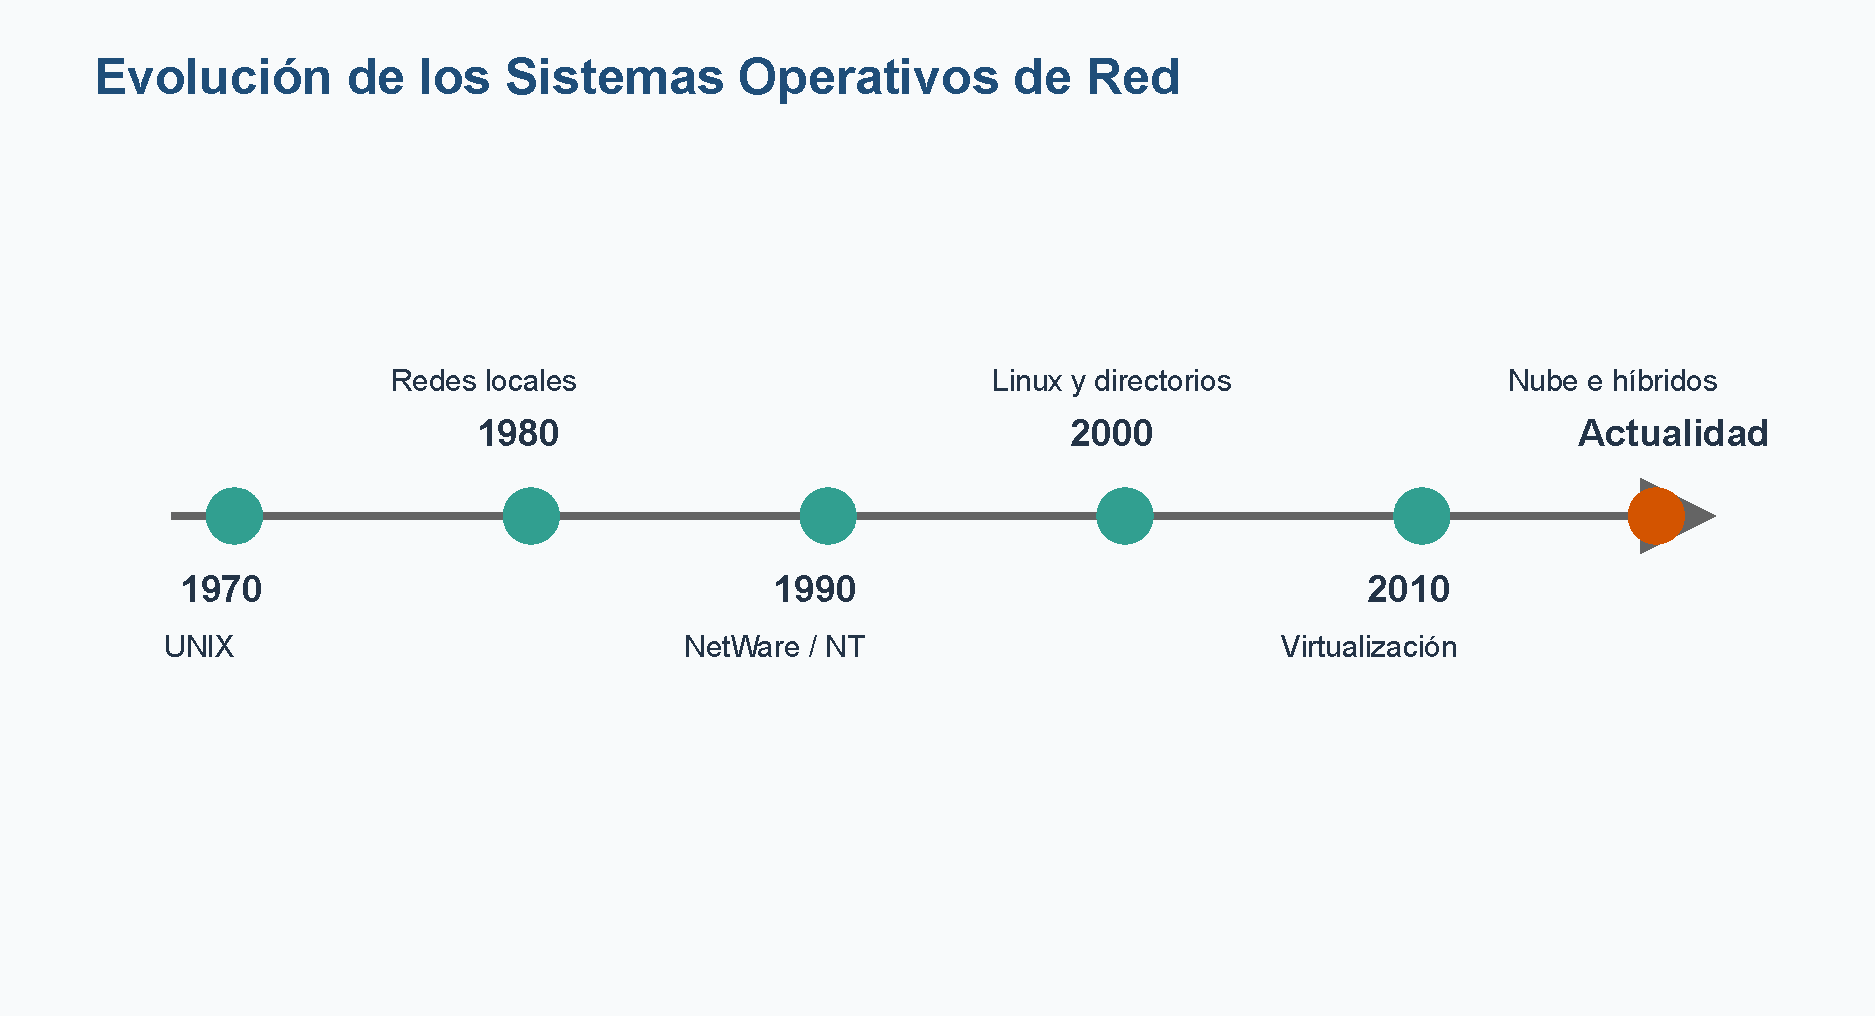
\includegraphics[width=0.95\linewidth,height=\textheight,keepaspectratio]{index_files/mediabag/capitulos/img/clase_03/fig_03_01_evolucion.pdf}

}

\caption{\label{fig-evolucion}Evolución de los Sistemas Operativos de
Red}

\end{figure}%

\section{Los primeros sistemas
multiusuario}\label{los-primeros-sistemas-multiusuario}

Durante las décadas de 1960 y 1970, las computadoras eran equipos
costosos y de gran tamaño. Para aprovecharlas, varios usuarios se
conectaban mediante terminales. En este contexto, UNIX introdujo
conceptos fundamentales:

\begin{itemize}
\tightlist
\item
  Multiusuario.
\item
  Multitarea.
\item
  Sistemas de archivos jerárquicos.
\item
  Permisos.
\item
  Administración remota.
\item
  Herramientas pequeñas que podían combinarse.
\end{itemize}

Estas ideas influyeron en numerosos sistemas posteriores.

\section{TCP/IP y la expansión de las
redes}\label{tcpip-y-la-expansiuxf3n-de-las-redes}

En la década de 1980, las implementaciones derivadas de BSD incorporaron
herramientas de comunicación basadas en TCP/IP y sockets. Esto facilitó
que diferentes equipos pudieran intercambiar información utilizando
estándares comunes.

TCP/IP terminó convirtiéndose en la base de Internet y de la mayoría de
redes actuales.

\section{Redes locales y Novell
NetWare}\label{redes-locales-y-novell-netware}

Con la expansión de las redes locales, empresas y universidades
comenzaron a compartir archivos e impresoras. Novell NetWare se
convirtió en una plataforma muy importante para estas tareas.

Su éxito se debió a que ofrecía:

\begin{itemize}
\tightlist
\item
  Buen rendimiento como servidor de archivos.
\item
  Administración de usuarios.
\item
  Servicios de impresión.
\item
  Compatibilidad con diferentes clientes.
\item
  Capacidad para operar en redes empresariales.
\end{itemize}

Aunque perdió presencia con el crecimiento de Windows Server y Linux,
NetWare representa una etapa clave en la historia de las redes.

\section{Windows NT y Windows Server}\label{windows-nt-y-windows-server}

Microsoft desarrolló Windows NT como una plataforma orientada a entornos
empresariales. Posteriormente evolucionó hacia la familia Windows
Server.

Estas plataformas incorporaron servicios como:

\begin{itemize}
\tightlist
\item
  Administración de dominios.
\item
  Active Directory.
\item
  Políticas de grupo.
\item
  Servicios de archivos e impresión.
\item
  DNS y DHCP.
\item
  Virtualización.
\item
  Administración remota.
\end{itemize}

Su integración con equipos Windows facilitó su adopción en muchas
organizaciones.

\section{El crecimiento de Linux}\label{el-crecimiento-de-linux}

Linux heredó la filosofía de UNIX y se desarrolló mediante una comunidad
internacional. Su estabilidad, flexibilidad y capacidad de adaptación lo
convirtieron en una opción ampliamente utilizada para servidores.

Hoy es común encontrar Linux en:

\begin{itemize}
\tightlist
\item
  Servidores web.
\item
  Bases de datos.
\item
  Centros de datos.
\item
  Plataformas de nube.
\item
  Dispositivos de red.
\item
  Supercomputadoras.
\item
  Sistemas embebidos.
\end{itemize}

\section{Virtualización, contenedores y
nube}\label{virtualizaciuxf3n-contenedores-y-nube}

Durante muchos años se instalaba un servidor físico para cada servicio.
Esto provocaba altos costos de energía, espacio y mantenimiento.

La virtualización permitió ejecutar varios servidores virtuales dentro
de un mismo equipo físico. Posteriormente, los contenedores facilitaron
empaquetar aplicaciones y dependencias de forma más ligera.

La computación en la nube añadió otra posibilidad: utilizar
infraestructura administrada por proveedores externos y pagar según la
capacidad consumida.

\begin{tcolorbox}[enhanced jigsaw, arc=.35mm, bottomrule=.15mm, breakable, colback=white, colframe=quarto-callout-note-color-frame, left=2mm, leftrule=.75mm, opacityback=0, rightrule=.15mm, toprule=.15mm]
\begin{minipage}[t]{5.5mm}
\textcolor{quarto-callout-note-color}{\faInfo}
\end{minipage}%
\begin{minipage}[t]{\textwidth - 5.5mm}

\vspace{-3mm}\textbf{Ingeniería en la vida real}\vspace{3mm}

Una universidad que antes necesitaba comprar un servidor físico para
cada aplicación puede ejecutar varios servidores virtuales en un clúster
local, mantener respaldos fuera del campus y utilizar servicios en la
nube para atender períodos de alta demanda.

\end{minipage}%
\end{tcolorbox}

\bookmarksetup{startatroot}

\chapter{Arquitecturas de red}\label{arquitecturas-de-red}

Una arquitectura de red describe cómo se organizan los equipos y cómo
solicitan o proporcionan servicios. Dos modelos fundamentales son:

\begin{itemize}
\tightlist
\item
  Punto a Punto.
\item
  Cliente/Servidor.
\end{itemize}

\bookmarksetup{startatroot}

\chapter{Arquitectura Punto a Punto}\label{arquitectura-punto-a-punto}

En una red \textbf{Punto a Punto}, también llamada \emph{Peer to Peer} o
P2P, los equipos poseen un nivel semejante. Cada computadora puede
solicitar recursos y también compartir los propios.

\begin{figure}

\centering{

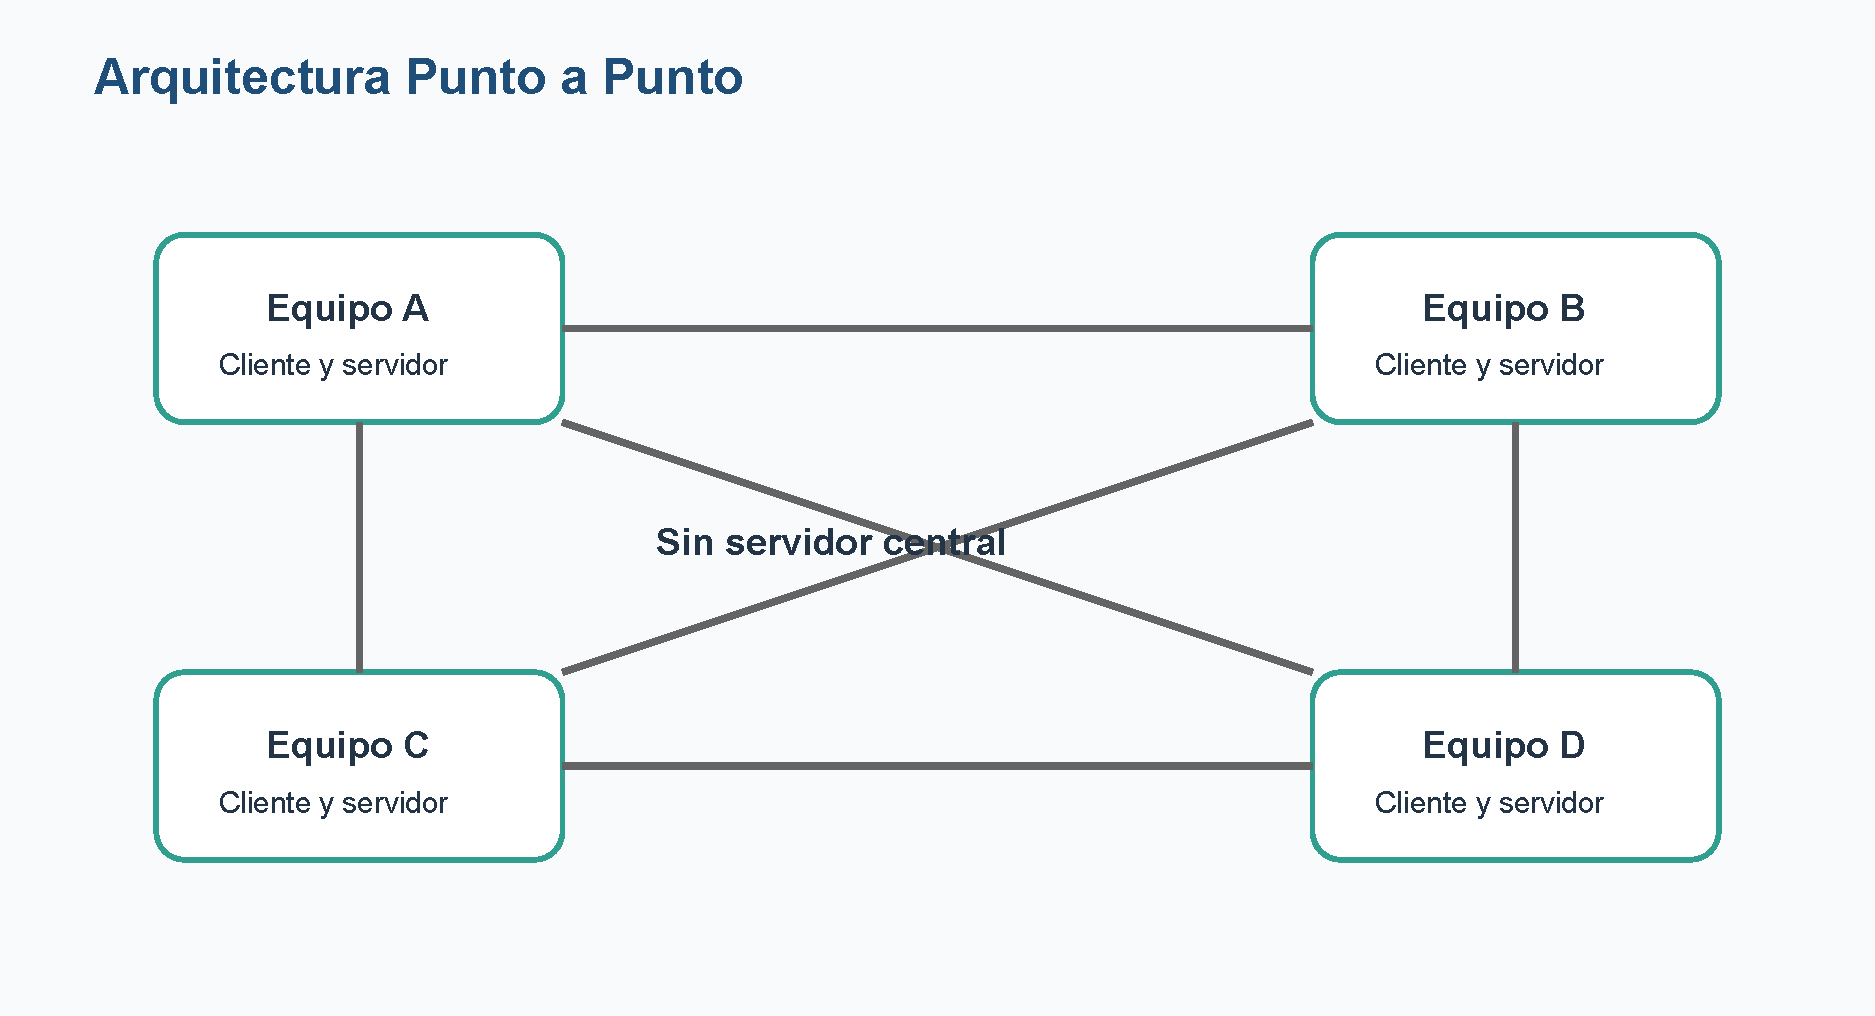
\includegraphics[width=0.9\linewidth,height=\textheight,keepaspectratio]{index_files/mediabag/capitulos/img/clase_03/fig_03_02_p2p.pdf}

}

\caption{\label{fig-p2p}Arquitectura Punto a Punto}

\end{figure}%

\section{Ejemplo}\label{ejemplo}

Un pequeño despacho posee cuatro computadoras. Una comparte la
impresora, otra contiene una carpeta de proyectos y las demás permiten
consultar ciertos documentos.

No existe un servidor central. Cada usuario decide qué comparte y con
quién.

\section{Ventajas}\label{ventajas}

\begin{itemize}
\tightlist
\item
  Bajo costo inicial.
\item
  Configuración relativamente sencilla.
\item
  No requiere un servidor dedicado.
\item
  Puede ser suficiente para pocos usuarios.
\item
  Permite compartir recursos rápidamente.
\end{itemize}

\section{Limitaciones}\label{limitaciones}

\begin{itemize}
\tightlist
\item
  La administración depende de cada equipo.
\item
  Es difícil mantener permisos consistentes.
\item
  Los respaldos quedan dispersos.
\item
  La seguridad es limitada.
\item
  Un recurso deja de estar disponible si se apaga el equipo que lo
  comparte.
\item
  El crecimiento aumenta rápidamente la complejidad.
\end{itemize}

\section{¿Cuándo puede utilizarse?}\label{cuuxe1ndo-puede-utilizarse}

Puede ser apropiada cuando:

\begin{itemize}
\tightlist
\item
  Hay pocos equipos.
\item
  La información no es crítica.
\item
  El presupuesto es muy reducido.
\item
  No se requiere administración centralizada.
\item
  La red es temporal o doméstica.
\end{itemize}

\begin{tcolorbox}[enhanced jigsaw, arc=.35mm, bottomrule=.15mm, breakable, colback=white, colframe=quarto-callout-warning-color-frame, left=2mm, leftrule=.75mm, opacityback=0, rightrule=.15mm, toprule=.15mm]
\begin{minipage}[t]{5.5mm}
\textcolor{quarto-callout-warning-color}{\faExclamationTriangle}
\end{minipage}%
\begin{minipage}[t]{\textwidth - 5.5mm}

\vspace{-3mm}\textbf{Cuidado}\vspace{3mm}

Que una red Punto a Punto sea fácil de instalar no significa que sea
adecuada para cualquier organización. Cuando existen datos sensibles,
muchos usuarios o necesidad de auditoría, este modelo suele quedarse
corto.

\end{minipage}%
\end{tcolorbox}

\bookmarksetup{startatroot}

\chapter{Arquitectura
Cliente/Servidor}\label{arquitectura-clienteservidor}

En una arquitectura \textbf{Cliente/Servidor}, uno o varios servidores
proporcionan servicios especializados y los equipos cliente los
solicitan.

\begin{figure}

\centering{

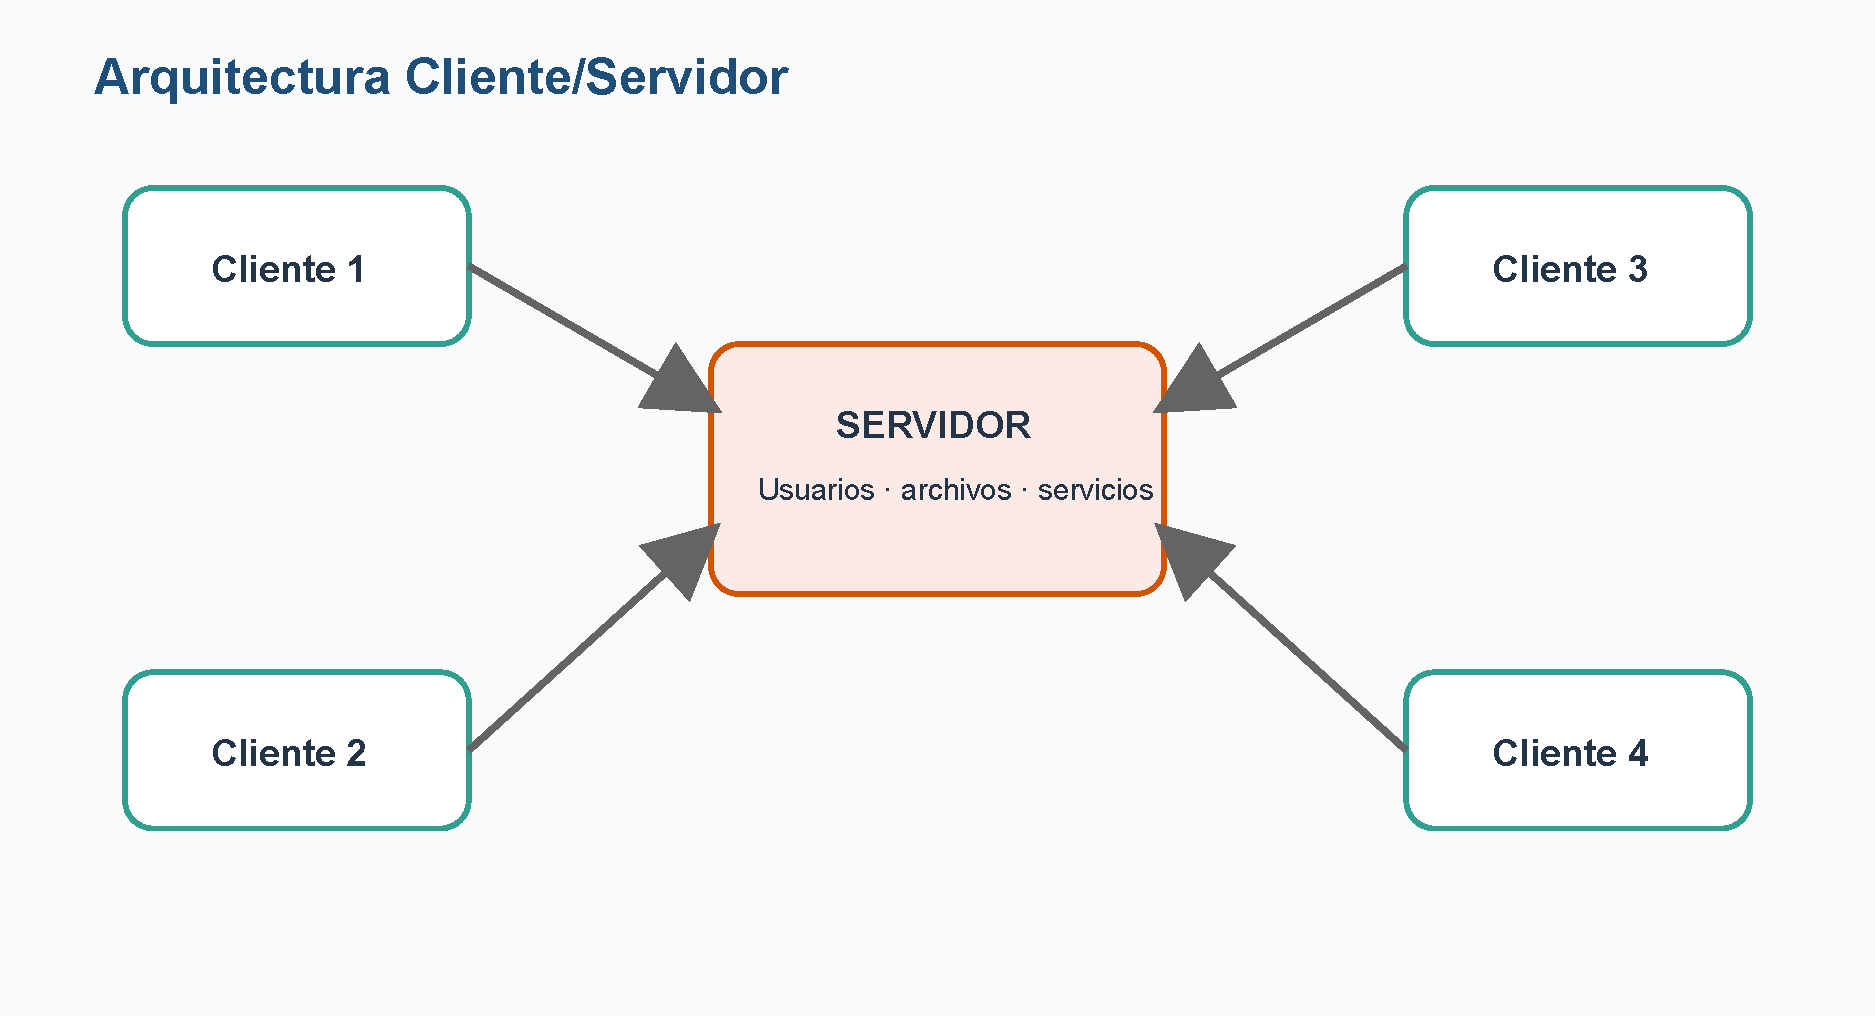
\includegraphics[width=0.9\linewidth,height=\textheight,keepaspectratio]{index_files/mediabag/capitulos/img/clase_03/fig_03_03_cliente_servidor.pdf}

}

\caption{\label{fig-cliente-servidor}Arquitectura Cliente/Servidor}

\end{figure}%

Un cliente puede ser:

\begin{itemize}
\tightlist
\item
  Una computadora de escritorio.
\item
  Una computadora portátil.
\item
  Un teléfono.
\item
  Una tableta.
\item
  Una aplicación.
\item
  Otro servidor.
\end{itemize}

El servidor procesa las solicitudes y responde de acuerdo con las
reglas, permisos y recursos disponibles.

\section{Ejemplo universitario}\label{ejemplo-universitario}

En un laboratorio, los estudiantes inician sesión desde diferentes
computadoras. Un servidor valida las credenciales, otro aloja el Campus
Virtual y otro contiene las bases de datos.

El estudiante observa una experiencia sencilla, pero la infraestructura
se encuentra distribuida y administrada.

\section{Ventajas}\label{ventajas-1}

\begin{itemize}
\tightlist
\item
  Administración centralizada.
\item
  Mayor control de usuarios.
\item
  Permisos consistentes.
\item
  Respaldos más sencillos.
\item
  Mejor capacidad de crecimiento.
\item
  Posibilidad de alta disponibilidad.
\item
  Auditoría y monitoreo centralizados.
\end{itemize}

\section{Limitaciones}\label{limitaciones-1}

\begin{itemize}
\tightlist
\item
  Mayor inversión inicial.
\item
  Requiere personal capacitado.
\item
  Los servidores son componentes críticos.
\item
  Una mala configuración puede afectar a muchos usuarios.
\item
  Se necesita planificar respaldo, redundancia y recuperación.
\end{itemize}

\section{Comparación general}\label{comparaciuxf3n-general}

{\def\LTcaptype{none} % do not increment counter
\begin{longtable}[]{@{}
  >{\raggedright\arraybackslash}p{(\linewidth - 4\tabcolsep) * \real{0.3333}}
  >{\raggedright\arraybackslash}p{(\linewidth - 4\tabcolsep) * \real{0.3333}}
  >{\raggedright\arraybackslash}p{(\linewidth - 4\tabcolsep) * \real{0.3333}}@{}}
\toprule\noalign{}
\begin{minipage}[b]{\linewidth}\raggedright
Característica
\end{minipage} & \begin{minipage}[b]{\linewidth}\raggedright
Punto a Punto
\end{minipage} & \begin{minipage}[b]{\linewidth}\raggedright
Cliente/Servidor
\end{minipage} \\
\midrule\noalign{}
\endhead
\bottomrule\noalign{}
\endlastfoot
Servidor dedicado & No es necesario & Generalmente sí \\
Administración & Distribuida & Centralizada \\
Seguridad & Básica & Mayor control \\
Escalabilidad & Baja & Alta \\
Respaldos & Dispersos & Centralizados \\
Costo inicial & Bajo & Medio o alto \\
Disponibilidad & Depende de cada equipo & Puede diseñarse con
redundancia \\
Uso típico & Hogares y oficinas pequeñas & Organizaciones medianas y
grandes \\
\end{longtable}
}

\begin{tcolorbox}[enhanced jigsaw, arc=.35mm, bottomrule=.15mm, breakable, colback=white, colframe=quarto-callout-tip-color-frame, left=2mm, leftrule=.75mm, opacityback=0, rightrule=.15mm, toprule=.15mm]
\begin{minipage}[t]{5.5mm}
\textcolor{quarto-callout-tip-color}{\faLightbulb}
\end{minipage}%
\begin{minipage}[t]{\textwidth - 5.5mm}

\vspace{-3mm}\textbf{Criterio de ingeniería}\vspace{3mm}

La arquitectura adecuada no es la más costosa ni la más moderna. Es la
que responde a los requerimientos de seguridad, capacidad,
disponibilidad, presupuesto y crecimiento de la organización.

\end{minipage}%
\end{tcolorbox}

\bookmarksetup{startatroot}

\chapter{Servicios que ofrece un Sistema Operativo de
Red}\label{servicios-que-ofrece-un-sistema-operativo-de-red}

Los servidores proporcionan \textbf{servicios}. Cada servicio resuelve
una necesidad específica de la red.

Entre los más importantes se encuentran:

\begin{itemize}
\tightlist
\item
  Autenticación.
\item
  DNS.
\item
  DHCP.
\item
  Compartición de archivos.
\item
  Impresión.
\item
  Directorio.
\item
  Bases de datos.
\item
  Aplicaciones web.
\item
  Correo electrónico.
\item
  Administración remota.
\end{itemize}

\bookmarksetup{startatroot}

\chapter{Servicio de autenticación}\label{servicio-de-autenticaciuxf3n}

La autenticación verifica la identidad de una persona o sistema.

El proceso básico es:

\begin{enumerate}
\def\labelenumi{\arabic{enumi}.}
\tightlist
\item
  El usuario proporciona una identidad.
\item
  Presenta una credencial.
\item
  El servidor valida la información.
\item
  Autoriza o rechaza el acceso.
\item
  Registra el evento.
\end{enumerate}

La contraseña es una credencial común, pero no es la única. También
pueden utilizarse:

\begin{itemize}
\tightlist
\item
  Códigos temporales.
\item
  Aplicaciones de autenticación.
\item
  Certificados.
\item
  Llaves físicas.
\item
  Datos biométricos.
\end{itemize}

\section{Autenticación y
autorización}\label{autenticaciuxf3n-y-autorizaciuxf3n}

Estos conceptos no significan lo mismo.

\begin{itemize}
\tightlist
\item
  \textbf{Autenticación:} confirma quién es el usuario.
\item
  \textbf{Autorización:} determina qué puede hacer.
\end{itemize}

Una persona puede autenticarse correctamente y aun así no tener permiso
para abrir una carpeta financiera.

\bookmarksetup{startatroot}

\chapter{Servicio DNS}\label{servicio-dns}

Las computadoras se comunican mediante direcciones IP, pero las personas
recuerdan mejor los nombres.

El \textbf{Domain Name System} traduce nombres como:

\begin{Shaded}
\begin{Highlighting}[]
\NormalTok{campus.umg.edu.gt}
\end{Highlighting}
\end{Shaded}

en una dirección IP asociada al servidor.

\begin{figure}

\centering{

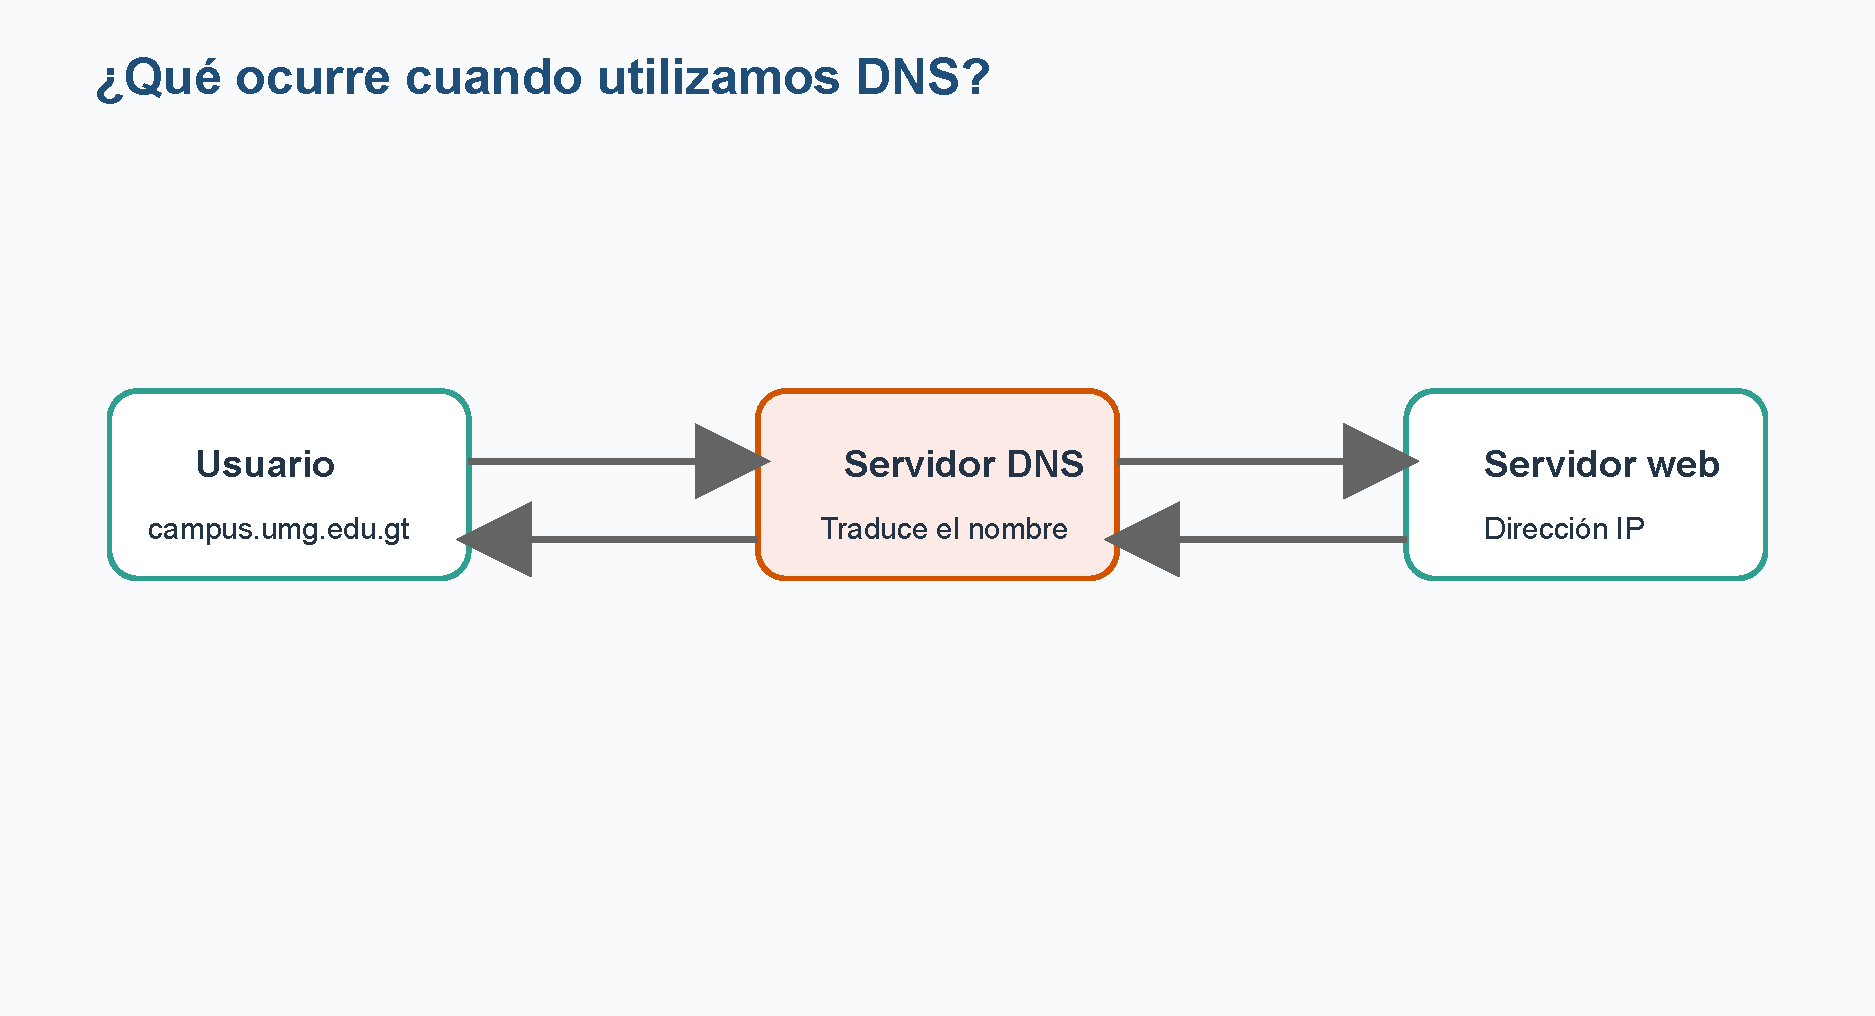
\includegraphics[width=0.9\linewidth,height=\textheight,keepaspectratio]{index_files/mediabag/capitulos/img/clase_03/fig_03_04_dns.pdf}

}

\caption{\label{fig-dns}Proceso simplificado de resolución DNS}

\end{figure}%

\section{Ejemplo de funcionamiento}\label{ejemplo-de-funcionamiento}

\begin{enumerate}
\def\labelenumi{\arabic{enumi}.}
\tightlist
\item
  El usuario escribe una dirección en el navegador.
\item
  El equipo consulta al servidor DNS.
\item
  El servidor DNS busca la dirección IP.
\item
  La respuesta regresa al equipo.
\item
  El navegador se comunica con el servidor web.
\end{enumerate}

\begin{tcolorbox}[enhanced jigsaw, arc=.35mm, bottomrule=.15mm, breakable, colback=white, colframe=quarto-callout-tip-color-frame, left=2mm, leftrule=.75mm, opacityback=0, rightrule=.15mm, toprule=.15mm]
\begin{minipage}[t]{5.5mm}
\textcolor{quarto-callout-tip-color}{\faLightbulb}
\end{minipage}%
\begin{minipage}[t]{\textwidth - 5.5mm}

\vspace{-3mm}\textbf{Idea central}\vspace{3mm}

DNS responde a la pregunta: \textbf{¿qué dirección IP corresponde a este
nombre?}

\end{minipage}%
\end{tcolorbox}

\section{¿Qué ocurriría sin DNS?}\label{quuxe9-ocurriruxeda-sin-dns}

Los usuarios tendrían que memorizar direcciones IP. Además, cualquier
cambio de dirección obligaría a comunicar la nueva configuración a todas
las personas y aplicaciones.

DNS desacopla el nombre lógico de la dirección física utilizada en un
momento determinado.

\bookmarksetup{startatroot}

\chapter{Servicio DHCP}\label{servicio-dhcp}

Cada dispositivo necesita una configuración de red. Entre otros datos:

\begin{itemize}
\tightlist
\item
  Dirección IP.
\item
  Máscara de subred.
\item
  Puerta de enlace.
\item
  Servidor DNS.
\end{itemize}

El \textbf{Dynamic Host Configuration Protocol} entrega estos valores
automáticamente.

\begin{figure}

\centering{

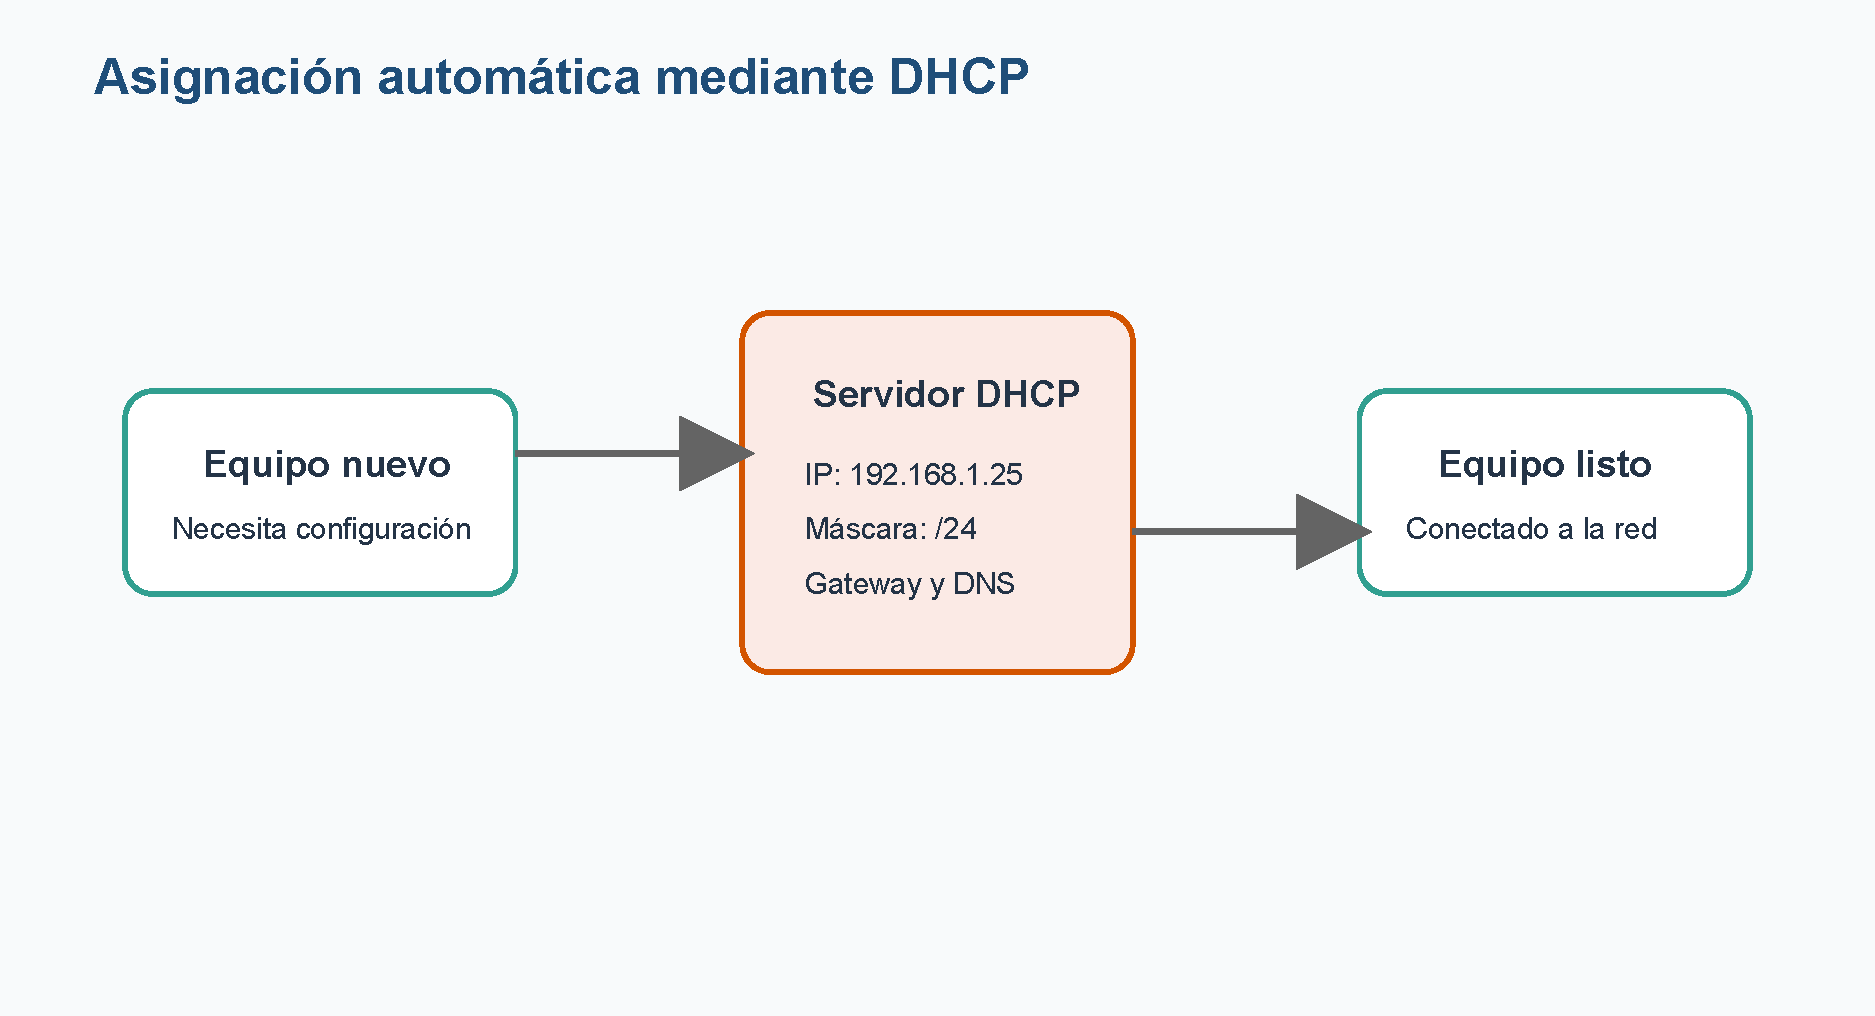
\includegraphics[width=0.9\linewidth,height=\textheight,keepaspectratio]{index_files/mediabag/capitulos/img/clase_03/fig_03_05_dhcp.pdf}

}

\caption{\label{fig-dhcp}Asignación automática mediante DHCP}

\end{figure}%

\section{Beneficios}\label{beneficios}

\begin{itemize}
\tightlist
\item
  Reduce errores manuales.
\item
  Evita direcciones duplicadas.
\item
  Facilita la incorporación de equipos.
\item
  Permite cambiar la configuración de forma centralizada.
\item
  Ahorra tiempo al personal técnico.
\end{itemize}

\section{\texorpdfstring{Concesión o
\emph{lease}}{Concesión o lease}}\label{concesiuxf3n-o-lease}

DHCP normalmente asigna una dirección durante un período determinado. El
equipo puede renovarla mientras permanece conectado.

Esto permite reutilizar las direcciones disponibles cuando los
dispositivos abandonan la red.

\begin{tcolorbox}[enhanced jigsaw, arc=.35mm, bottomrule=.15mm, breakable, colback=white, colframe=quarto-callout-note-color-frame, left=2mm, leftrule=.75mm, opacityback=0, rightrule=.15mm, toprule=.15mm]
\begin{minipage}[t]{5.5mm}
\textcolor{quarto-callout-note-color}{\faInfo}
\end{minipage}%
\begin{minipage}[t]{\textwidth - 5.5mm}

\vspace{-3mm}\textbf{DNS y DHCP trabajan juntos}\vspace{3mm}

DHCP puede entregar al equipo la dirección del servidor DNS. DNS permite
localizar servicios por nombre. Uno configura la comunicación y el otro
facilita encontrar los recursos.

\end{minipage}%
\end{tcolorbox}

\bookmarksetup{startatroot}

\chapter{Servicio de archivos}\label{servicio-de-archivos}

Un servidor de archivos almacena información de forma centralizada y la
comparte según los permisos definidos.

\section{Ventajas}\label{ventajas-2}

\begin{itemize}
\tightlist
\item
  Facilita los respaldos.
\item
  Reduce la dispersión de documentos.
\item
  Permite trabajo colaborativo.
\item
  Mejora el control de acceso.
\item
  Facilita auditoría y recuperación.
\item
  Evita depender de un equipo personal.
\end{itemize}

\section{Ejemplo de estructura}\label{ejemplo-de-estructura}

\begin{Shaded}
\begin{Highlighting}[]
\NormalTok{/Institución}
\NormalTok{├── Dirección}
\NormalTok{├── Administración}
\NormalTok{├── Docentes}
\NormalTok{├── Estudiantes}
\NormalTok{├── Biblioteca}
\NormalTok{└── Soporte}
\end{Highlighting}
\end{Shaded}

Cada carpeta puede tener permisos distintos.

\section{Riesgos que deben
administrarse}\label{riesgos-que-deben-administrarse}

\begin{itemize}
\tightlist
\item
  Eliminación accidental.
\item
  Modificaciones no autorizadas.
\item
  Uso excesivo del almacenamiento.
\item
  Archivos maliciosos.
\item
  Acceso desde dispositivos no autorizados.
\item
  Falta de versiones o respaldos.
\end{itemize}

\bookmarksetup{startatroot}

\chapter{Servicio de impresión}\label{servicio-de-impresiuxf3n}

El servidor de impresión administra impresoras compartidas y las colas
de trabajos.

Puede:

\begin{itemize}
\tightlist
\item
  Publicar impresoras.
\item
  Controlar quién puede imprimir.
\item
  Priorizar trabajos.
\item
  Registrar consumo.
\item
  Instalar controladores.
\item
  Pausar o cancelar documentos.
\end{itemize}

En una organización grande, esta administración evita instalar y
configurar cada impresora de forma independiente en todos los equipos.

\bookmarksetup{startatroot}

\chapter{Servicio de directorio}\label{servicio-de-directorio}

Un servicio de directorio almacena y organiza objetos de la red.

Entre ellos:

\begin{itemize}
\tightlist
\item
  Usuarios.
\item
  Grupos.
\item
  Equipos.
\item
  Impresoras.
\item
  Unidades organizativas.
\item
  Políticas.
\item
  Recursos compartidos.
\end{itemize}

Active Directory es una implementación conocida en entornos Microsoft.
En otros contextos pueden utilizarse LDAP y herramientas compatibles.

Un directorio no es únicamente una lista de nombres. Permite consultar
relaciones, aplicar políticas y administrar identidades a gran escala.

\bookmarksetup{startatroot}

\chapter{Administración remota}\label{administraciuxf3n-remota}

Los servidores suelen encontrarse en centros de datos, cuartos técnicos
o servicios en la nube. Por eso deben poder administrarse sin estar
físicamente frente a ellos.

La administración remota permite:

\begin{itemize}
\tightlist
\item
  Revisar el estado del sistema.
\item
  Instalar actualizaciones.
\item
  Consultar registros.
\item
  Reiniciar servicios.
\item
  Modificar configuraciones.
\item
  Automatizar tareas.
\item
  Atender incidentes.
\end{itemize}

Debe utilizar canales seguros, cuentas individuales y registros de
auditoría.

\bookmarksetup{startatroot}

\chapter{¿Qué ocurre detrás de escena al iniciar
sesión?}\label{quuxe9-ocurre-detruxe1s-de-escena-al-iniciar-sesiuxf3n}

\begin{figure}

\centering{

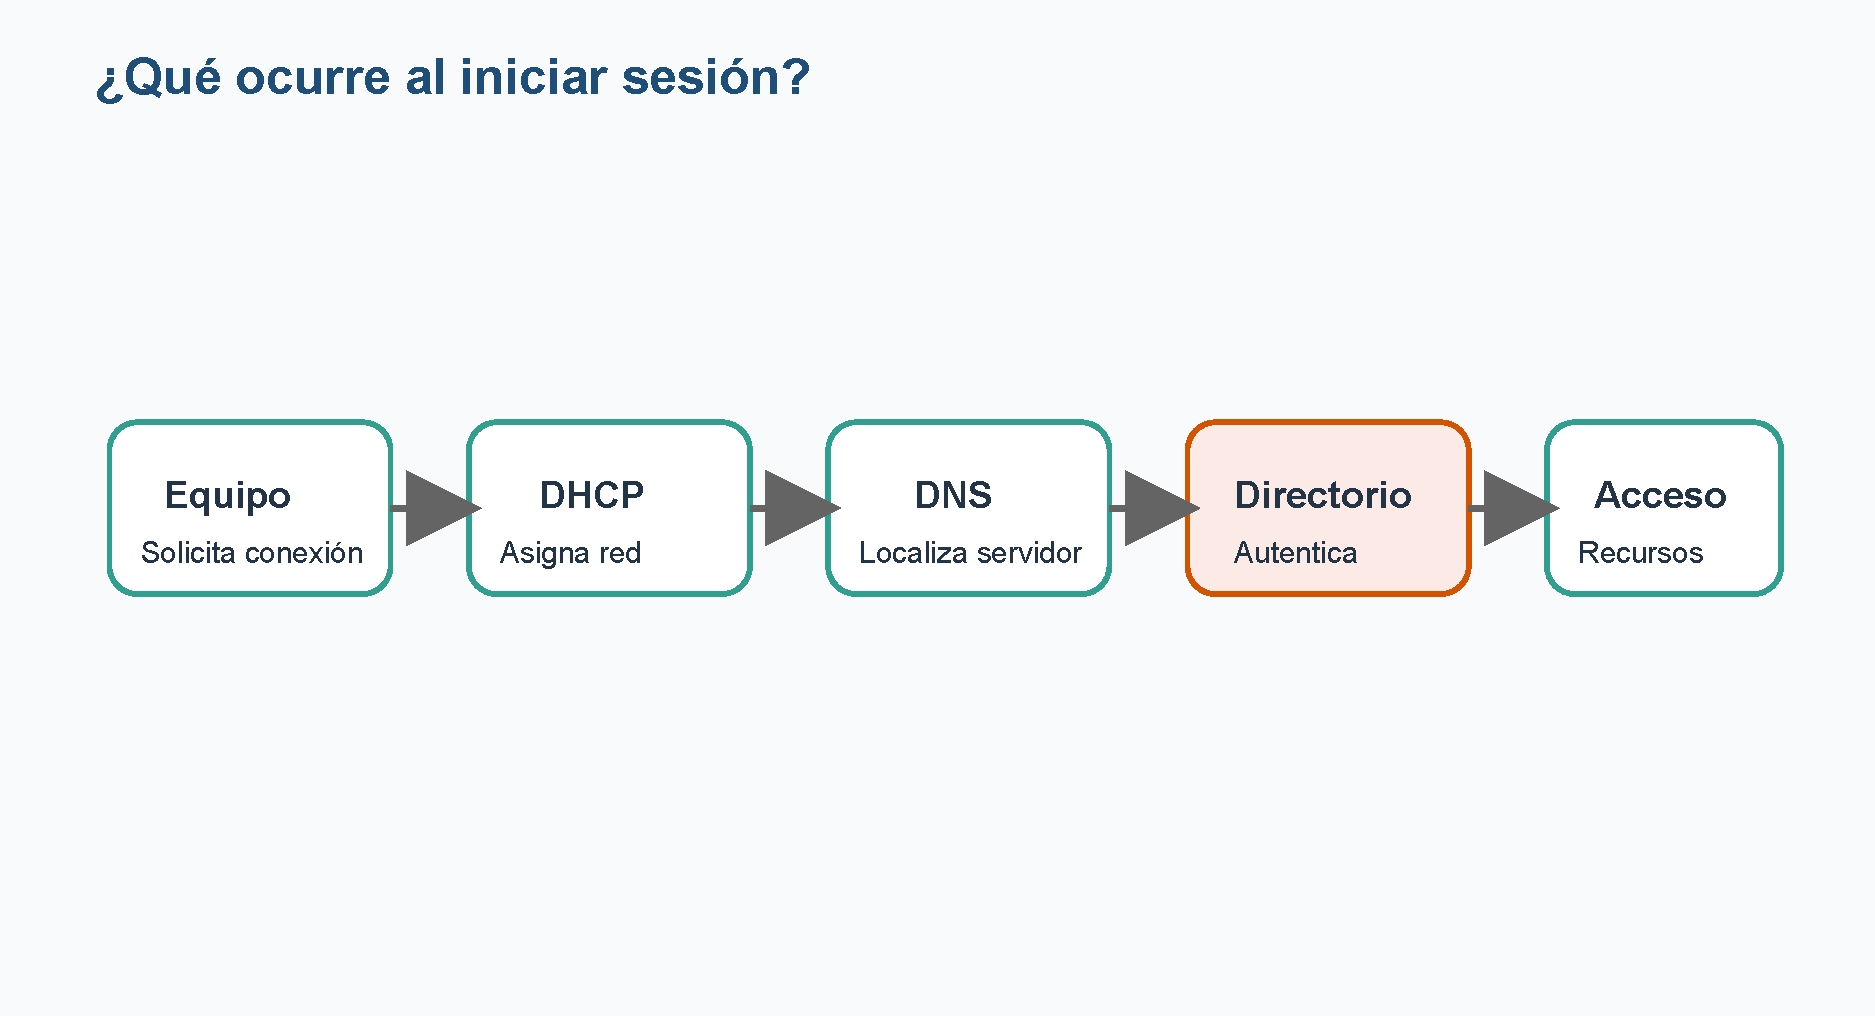
\includegraphics[width=0.95\linewidth,height=\textheight,keepaspectratio]{index_files/mediabag/capitulos/img/clase_03/fig_03_10_flujo.pdf}

}

\caption{\label{fig-flujo-login}Flujo simplificado de inicio de sesión}

\end{figure}%

Un inicio de sesión puede involucrar los siguientes pasos:

\begin{enumerate}
\def\labelenumi{\arabic{enumi}.}
\tightlist
\item
  El equipo se conecta a la red.
\item
  DHCP proporciona la configuración necesaria.
\item
  DNS localiza el servidor de autenticación.
\item
  El usuario presenta sus credenciales.
\item
  El servicio de directorio valida la identidad.
\item
  El sistema consulta grupos y permisos.
\item
  Se aplican políticas.
\item
  Se habilitan carpetas, impresoras y aplicaciones autorizadas.
\item
  El evento queda registrado.
\end{enumerate}

Para el usuario, el proceso dura unos segundos. Para el administrador,
representa una cadena de servicios que debe funcionar correctamente.

\bookmarksetup{startatroot}

\chapter{Usuarios, grupos y permisos}\label{usuarios-grupos-y-permisos}

La seguridad de una red se apoya en tres componentes relacionados:

\begin{itemize}
\tightlist
\item
  Usuarios.
\item
  Grupos.
\item
  Permisos.
\end{itemize}

\begin{figure}

\centering{

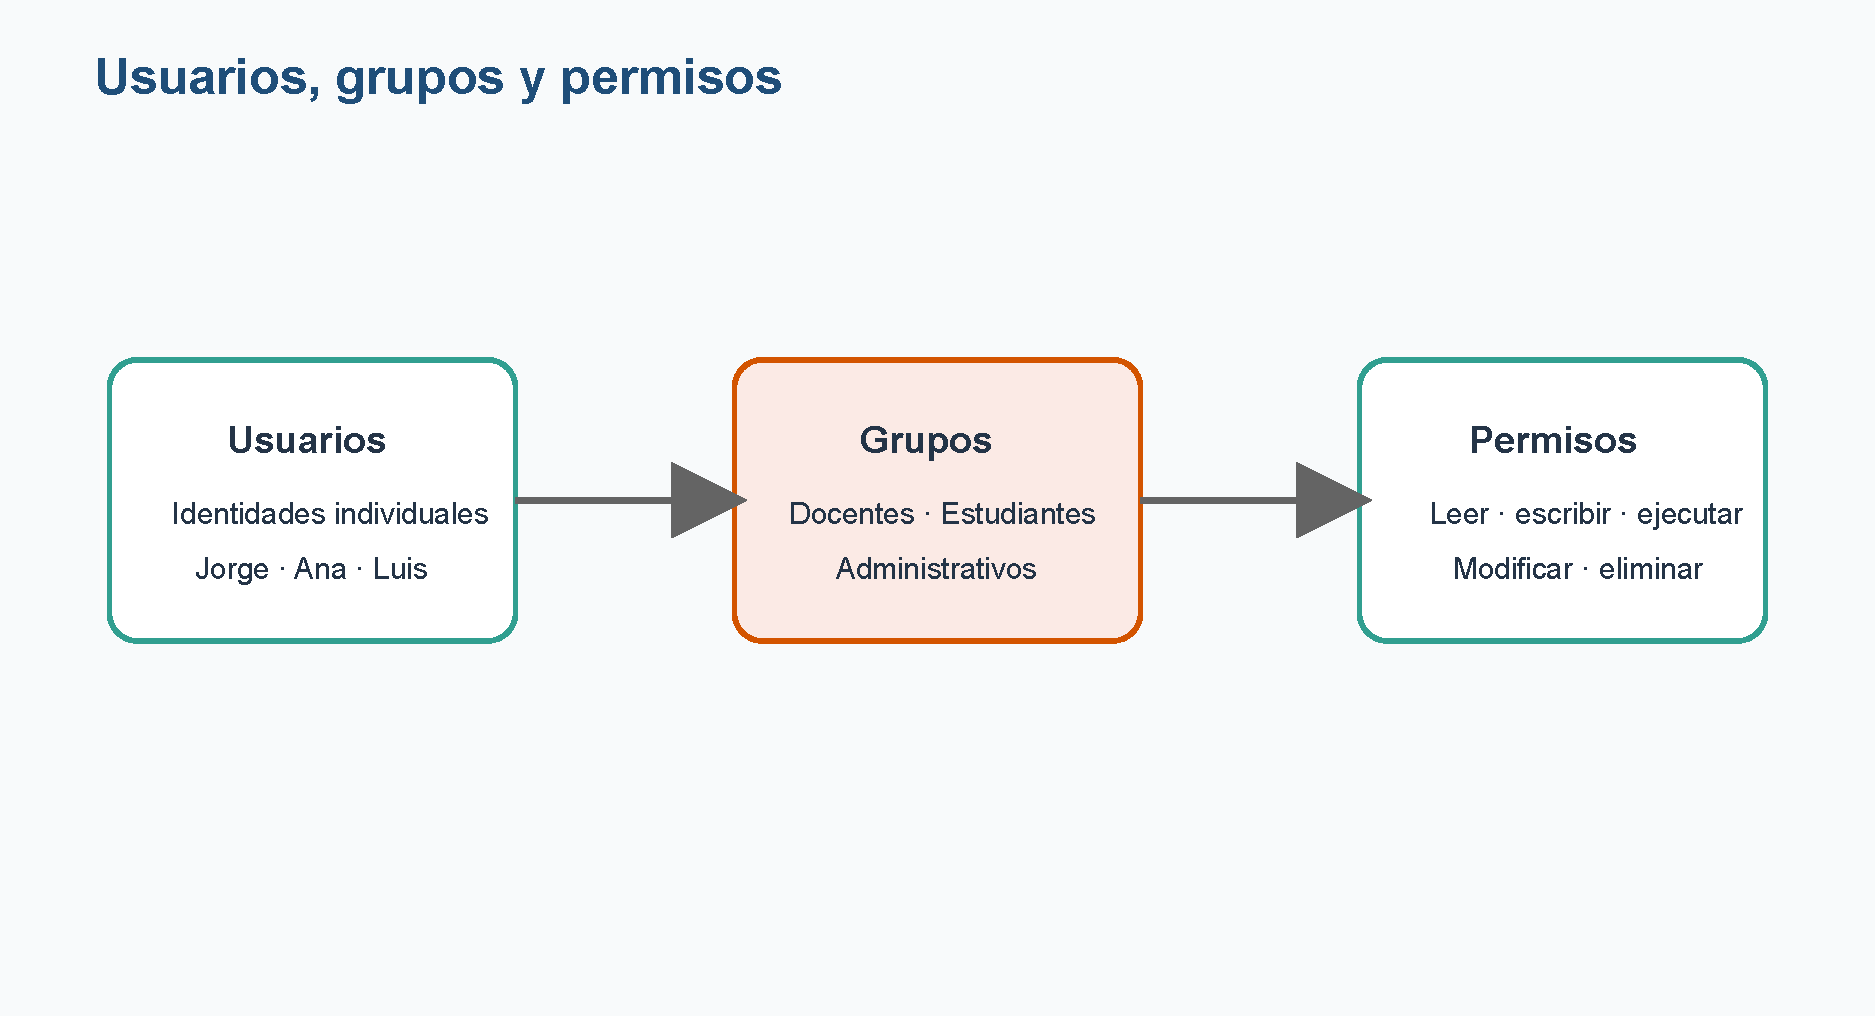
\includegraphics[width=0.9\linewidth,height=\textheight,keepaspectratio]{index_files/mediabag/capitulos/img/clase_03/fig_03_06_usuarios.pdf}

}

\caption{\label{fig-usuarios}Relación entre usuarios, grupos y permisos}

\end{figure}%

\bookmarksetup{startatroot}

\chapter{Usuarios}\label{usuarios}

Un usuario representa una identidad digital. Puede corresponder a:

\begin{itemize}
\tightlist
\item
  Una persona.
\item
  Un servicio.
\item
  Una aplicación.
\item
  Un equipo.
\item
  Una cuenta temporal.
\end{itemize}

Una cuenta debería ser individual cuando se necesita responsabilidad y
auditoría.

\section{¿Por qué evitar cuentas
compartidas?}\label{por-quuxe9-evitar-cuentas-compartidas}

Si varias personas utilizan la misma cuenta:

\begin{itemize}
\tightlist
\item
  No se sabe quién realizó una acción.
\item
  Es difícil revocar el acceso de una sola persona.
\item
  La contraseña se comparte ampliamente.
\item
  La auditoría pierde valor.
\item
  Aumenta el riesgo de uso indebido.
\end{itemize}

\bookmarksetup{startatroot}

\chapter{Grupos}\label{grupos}

Un grupo reúne usuarios con funciones semejantes.

Ejemplos:

\begin{itemize}
\tightlist
\item
  Docentes.
\item
  Estudiantes.
\item
  Tesorería.
\item
  Recursos Humanos.
\item
  Soporte Técnico.
\item
  Administradores.
\end{itemize}

En lugar de asignar permisos persona por persona, se asignan al grupo y
luego se incorporan los usuarios correspondientes.

\section{Ventaja administrativa}\label{ventaja-administrativa}

Si ingresan diez docentes nuevos, basta con agregarlos al grupo
\textbf{Docentes} para que reciban los permisos establecidos.

Si una persona cambia de puesto, se modifican sus grupos en lugar de
revisar recurso por recurso.

\bookmarksetup{startatroot}

\chapter{Permisos}\label{permisos}

Los permisos determinan las acciones autorizadas sobre un recurso.

{\def\LTcaptype{none} % do not increment counter
\begin{longtable}[]{@{}ll@{}}
\toprule\noalign{}
Permiso & Descripción \\
\midrule\noalign{}
\endhead
\bottomrule\noalign{}
\endlastfoot
Lectura & Consultar información \\
Escritura & Modificar contenido \\
Crear & Agregar nuevos elementos \\
Ejecutar & Iniciar un programa o proceso \\
Eliminar & Borrar información \\
Administrar & Cambiar permisos o configuración \\
\end{longtable}
}

\section{Caso: carpeta de
calificaciones}\label{caso-carpeta-de-calificaciones}

{\def\LTcaptype{none} % do not increment counter
\begin{longtable}[]{@{}lrrr@{}}
\toprule\noalign{}
Rol & Leer & Escribir & Eliminar \\
\midrule\noalign{}
\endhead
\bottomrule\noalign{}
\endlastfoot
Coordinación & Sí & Sí & Sí \\
Docente & Sí & Sí & Según política \\
Estudiante & Solo sus resultados & No & No \\
Visitante & No & No & No \\
\end{longtable}
}

\bookmarksetup{startatroot}

\chapter{Principio del mínimo
privilegio}\label{principio-del-muxednimo-privilegio}

Este principio indica que una persona debe recibir únicamente los
permisos necesarios para realizar su trabajo.

\section{Ejemplos}\label{ejemplos}

\begin{itemize}
\tightlist
\item
  Un estudiante no necesita administrar servidores.
\item
  Una recepcionista no necesita modificar respaldos.
\item
  Un técnico de soporte no necesita consultar salarios.
\item
  Una aplicación web no debería conectarse a la base de datos como
  administrador.
\end{itemize}

\begin{tcolorbox}[enhanced jigsaw, arc=.35mm, bottomrule=.15mm, breakable, colback=white, colframe=quarto-callout-important-color-frame, left=2mm, leftrule=.75mm, opacityback=0, rightrule=.15mm, toprule=.15mm]
\begin{minipage}[t]{5.5mm}
\textcolor{quarto-callout-important-color}{\faExclamation}
\end{minipage}%
\begin{minipage}[t]{\textwidth - 5.5mm}

\vspace{-3mm}\textbf{Idea central}\vspace{3mm}

Dar permisos ``por si acaso'' facilita el trabajo al inicio, pero
aumenta el riesgo. El acceso debe justificarse por una necesidad real.

\end{minipage}%
\end{tcolorbox}

\bookmarksetup{startatroot}

\chapter{Plataformas de Sistemas Operativos de
Red}\label{plataformas-de-sistemas-operativos-de-red}

No existe una plataforma universalmente superior. La selección depende
de requisitos, experiencia del equipo, aplicaciones, presupuesto y
soporte.

\bookmarksetup{startatroot}

\chapter{Windows Server}\label{windows-server}

Windows Server está orientado a entornos empresariales y se integra
estrechamente con estaciones de trabajo Windows.

Entre sus capacidades se encuentran:

\begin{itemize}
\tightlist
\item
  Active Directory.
\item
  DNS y DHCP.
\item
  Políticas de grupo.
\item
  Servicios de archivos.
\item
  Servicios de impresión.
\item
  Virtualización.
\item
  Administración gráfica y mediante línea de comandos.
\item
  Integración con servicios Microsoft.
\end{itemize}

\section{Fortalezas}\label{fortalezas}

\begin{itemize}
\tightlist
\item
  Administración centralizada.
\item
  Amplia adopción empresarial.
\item
  Integración con escritorios Windows.
\item
  Herramientas gráficas.
\item
  Ecosistema de soporte.
\end{itemize}

\section{Consideraciones}\label{consideraciones}

\begin{itemize}
\tightlist
\item
  Licenciamiento.
\item
  Requisitos de hardware.
\item
  Necesidad de planificar actualizaciones.
\item
  Dependencia de herramientas y conocimientos especializados.
\end{itemize}

\bookmarksetup{startatroot}

\chapter{Linux Server}\label{linux-server}

Linux está disponible mediante diferentes distribuciones.

Algunas están orientadas a estabilidad empresarial, otras a facilidad de
uso o flexibilidad.

Es común utilizar Linux para:

\begin{itemize}
\tightlist
\item
  Servidores web.
\item
  Bases de datos.
\item
  DNS y DHCP.
\item
  Almacenamiento.
\item
  Contenedores.
\item
  Automatización.
\item
  Infraestructura en la nube.
\end{itemize}

\section{Fortalezas}\label{fortalezas-1}

\begin{itemize}
\tightlist
\item
  Flexibilidad.
\item
  Estabilidad.
\item
  Automatización.
\item
  Amplia comunidad.
\item
  Posibilidad de utilizar herramientas abiertas.
\item
  Buen desempeño en servidores.
\end{itemize}

\section{Consideraciones}\label{consideraciones-1}

\begin{itemize}
\tightlist
\item
  La administración puede requerir experiencia en línea de comandos.
\item
  Las distribuciones poseen ciclos de soporte diferentes.
\item
  Debe seleccionarse una versión adecuada para producción.
\item
  La flexibilidad también exige disciplina de configuración.
\end{itemize}

\bookmarksetup{startatroot}

\chapter{UNIX}\label{unix}

UNIX representa una familia y una filosofía de sistemas que influyó
profundamente en la informática moderna.

Sus características históricas incluyen:

\begin{itemize}
\tightlist
\item
  Multiusuario.
\item
  Multitarea.
\item
  Portabilidad.
\item
  Permisos robustos.
\item
  Herramientas modulares.
\item
  Administración mediante texto y comandos.
\end{itemize}

Algunas variantes comerciales continúan utilizándose en ambientes
especializados y sistemas críticos.

\bookmarksetup{startatroot}

\chapter{Infraestructuras híbridas}\label{infraestructuras-huxedbridas}

En la práctica, muchas organizaciones combinan plataformas.

Ejemplo:

\begin{itemize}
\tightlist
\item
  Windows Server para usuarios y políticas.
\item
  Linux para aplicaciones web.
\item
  Un dispositivo especializado para firewall.
\item
  Servicios de respaldo en la nube.
\item
  Bases de datos alojadas en otra plataforma.
\end{itemize}

\begin{tcolorbox}[enhanced jigsaw, arc=.35mm, bottomrule=.15mm, breakable, colback=white, colframe=quarto-callout-tip-color-frame, left=2mm, leftrule=.75mm, opacityback=0, rightrule=.15mm, toprule=.15mm]
\begin{minipage}[t]{5.5mm}
\textcolor{quarto-callout-tip-color}{\faLightbulb}
\end{minipage}%
\begin{minipage}[t]{\textwidth - 5.5mm}

\vspace{-3mm}\textbf{Criterio profesional}\vspace{3mm}

El trabajo del ingeniero no consiste en defender una marca. Consiste en
justificar una decisión técnica con base en necesidades, riesgos, costos
y capacidades.

\end{minipage}%
\end{tcolorbox}

\bookmarksetup{startatroot}

\chapter{Roles de un servidor}\label{roles-de-un-servidor}

Un \textbf{rol} describe la función que cumple un servidor dentro de la
infraestructura.

\begin{figure}

\centering{

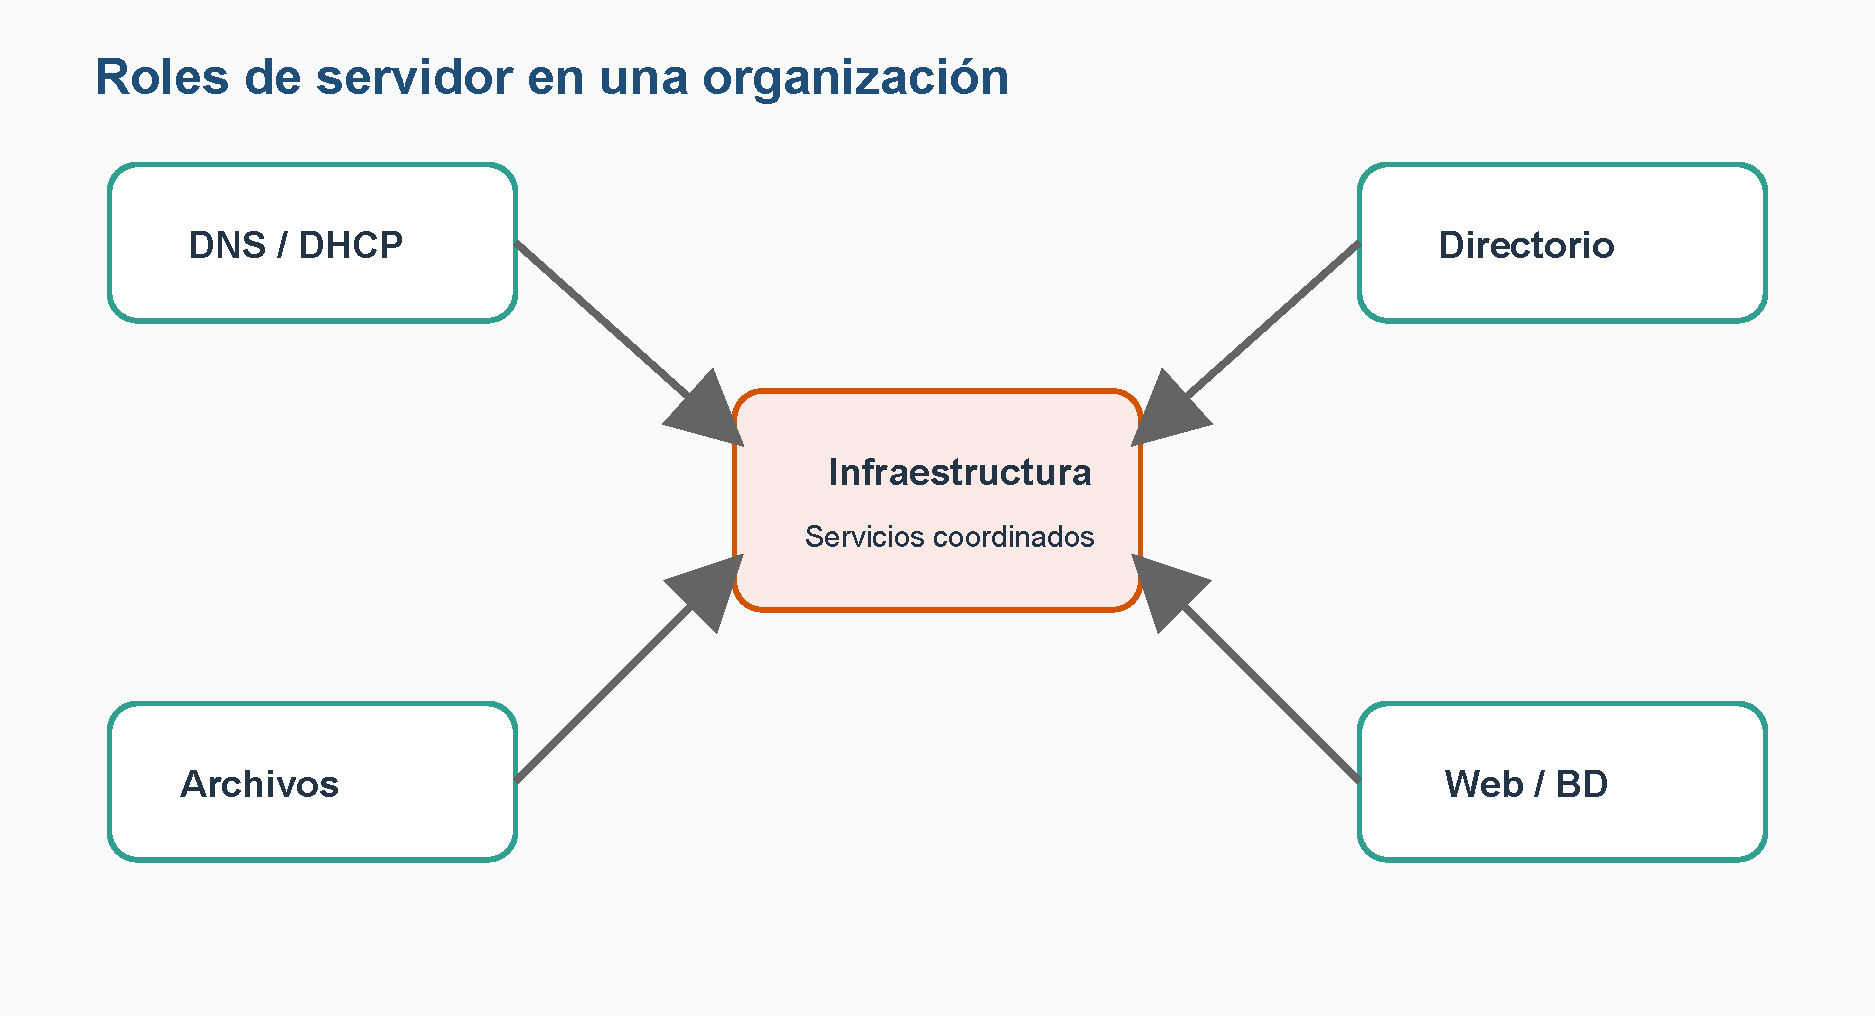
\includegraphics[width=0.9\linewidth,height=\textheight,keepaspectratio]{index_files/mediabag/capitulos/img/clase_03/fig_03_07_roles.pdf}

}

\caption{\label{fig-roles}Roles de servidor}

\end{figure}%

\bookmarksetup{startatroot}

\chapter{Servidor de archivos}\label{servidor-de-archivos}

Centraliza documentos y los comparte según permisos.

\bookmarksetup{startatroot}

\chapter{Servidor de impresión}\label{servidor-de-impresiuxf3n}

Administra impresoras, colas y control de acceso.

\bookmarksetup{startatroot}

\chapter{Servidor web}\label{servidor-web}

Publica sitios y aplicaciones mediante protocolos web.

Programas conocidos incluyen Apache, Nginx e IIS.

\bookmarksetup{startatroot}

\chapter{Servidor de bases de datos}\label{servidor-de-bases-de-datos}

Almacena información estructurada y procesa consultas.

Puede utilizar motores como:

\begin{itemize}
\tightlist
\item
  PostgreSQL.
\item
  MySQL.
\item
  Microsoft SQL Server.
\item
  Oracle Database.
\end{itemize}

\bookmarksetup{startatroot}

\chapter{Servidor de correo}\label{servidor-de-correo}

Gestiona envío, recepción, buzones y autenticación del correo
institucional.

\bookmarksetup{startatroot}

\chapter{Servidor DNS}\label{servidor-dns}

Traduce nombres en direcciones IP.

\bookmarksetup{startatroot}

\chapter{Servidor DHCP}\label{servidor-dhcp}

Entrega automáticamente la configuración de red.

\bookmarksetup{startatroot}

\chapter{Controlador de dominio o servidor de
identidad}\label{controlador-de-dominio-o-servidor-de-identidad}

Administra usuarios, grupos, equipos y políticas de autenticación.

\bookmarksetup{startatroot}

\chapter{Servidor de aplicaciones}\label{servidor-de-aplicaciones}

Ejecuta lógica de negocio utilizada por los clientes.

\bookmarksetup{startatroot}

\chapter{Servidor de respaldo}\label{servidor-de-respaldo}

Recibe y conserva copias de seguridad para recuperación.

\bookmarksetup{startatroot}

\chapter{Servidor de monitoreo}\label{servidor-de-monitoreo}

Supervisa disponibilidad, uso de recursos, eventos y alertas.

\bookmarksetup{startatroot}

\chapter{¿Un servidor puede tener varios
roles?}\label{un-servidor-puede-tener-varios-roles}

Sí. En una organización pequeña, un servidor puede proporcionar DNS,
DHCP, archivos y autenticación.

Sin embargo, concentrar demasiados roles puede generar riesgos:

\begin{itemize}
\tightlist
\item
  Una falla afecta múltiples servicios.
\item
  El mantenimiento requiere detener varias funciones.
\item
  Aumenta la superficie de ataque.
\item
  Se dificulta identificar problemas.
\item
  Los recursos pueden competir entre sí.
\end{itemize}

En organizaciones grandes se distribuyen los roles y se utilizan
mecanismos de redundancia.

\bookmarksetup{startatroot}

\chapter{Infraestructura simplificada de una
universidad}\label{infraestructura-simplificada-de-una-universidad}

\begin{figure}

\centering{

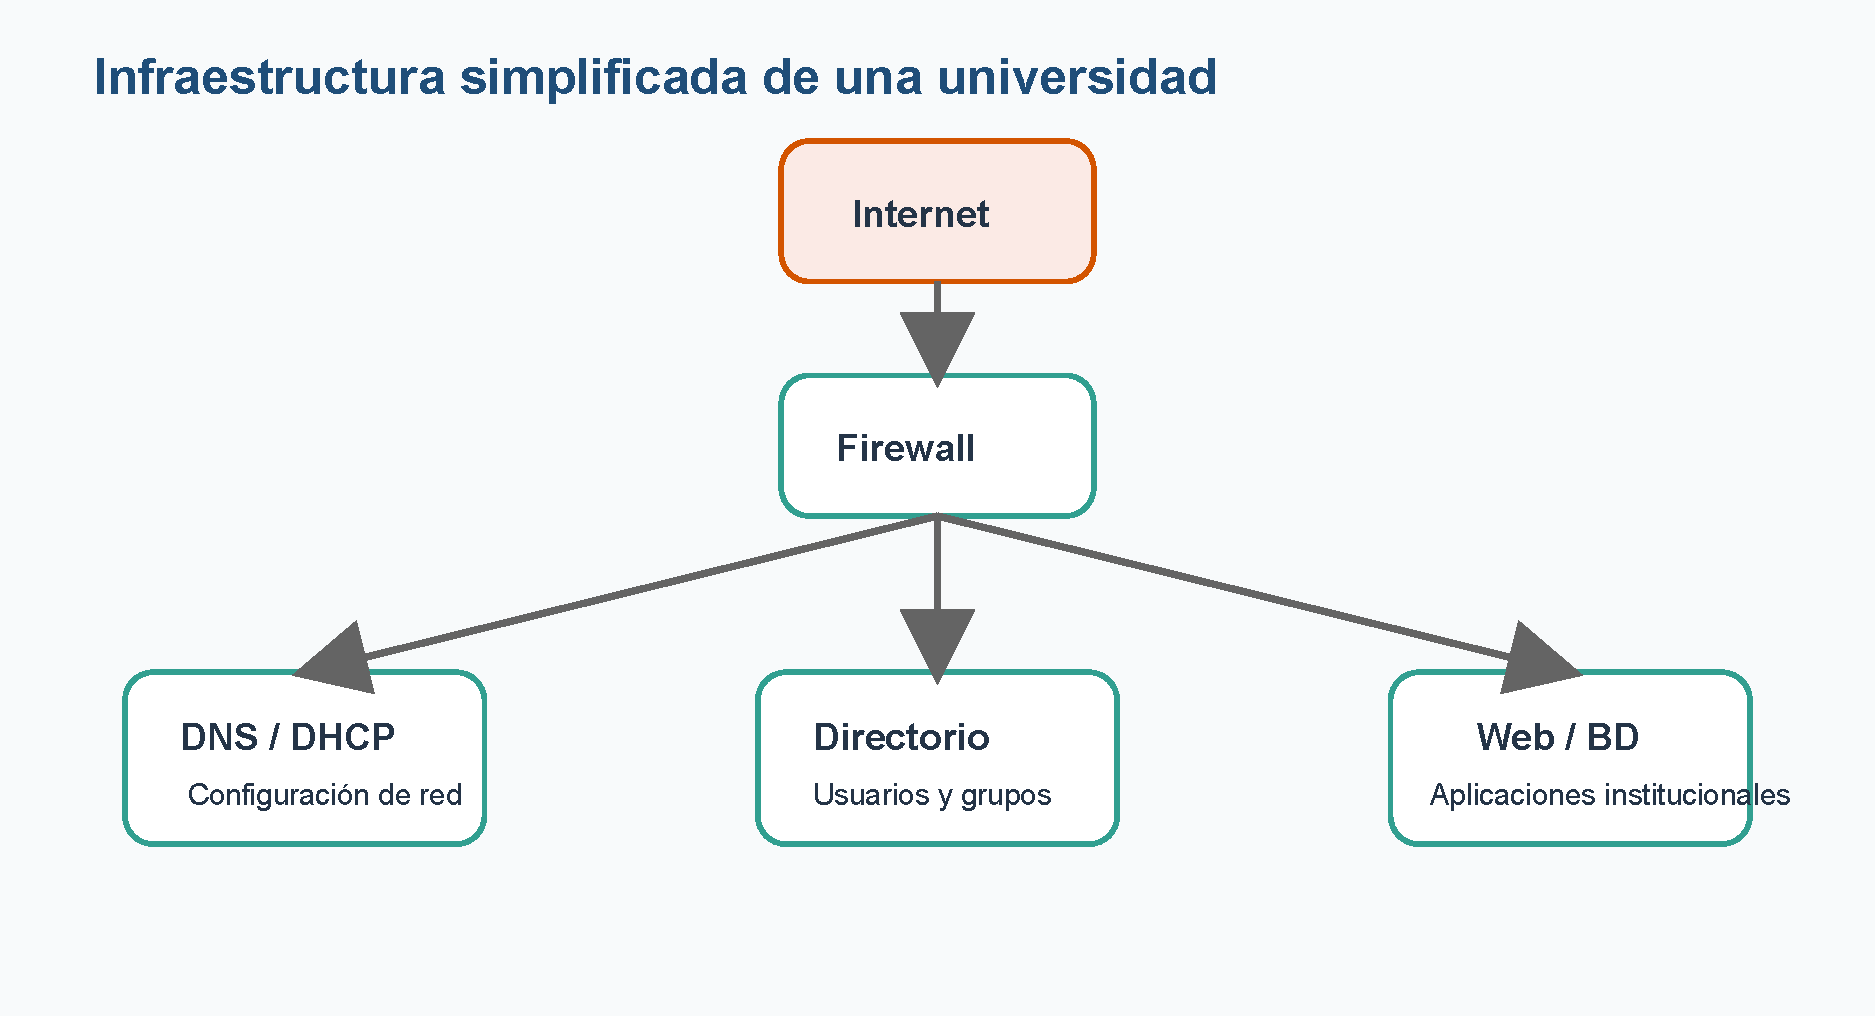
\includegraphics[width=0.95\linewidth,height=\textheight,keepaspectratio]{index_files/mediabag/capitulos/img/clase_03/fig_03_09_infraestructura.pdf}

}

\caption{\label{fig-infraestructura}Infraestructura universitaria
simplificada}

\end{figure}%

Una infraestructura universitaria puede incluir:

\begin{itemize}
\tightlist
\item
  Conexión a Internet.
\item
  Firewall.
\item
  DNS y DHCP.
\item
  Servicio de identidad.
\item
  Servidor de archivos.
\item
  Aplicaciones web.
\item
  Bases de datos.
\item
  Respaldos.
\item
  Monitoreo.
\end{itemize}

La arquitectura real dependerá del tamaño y las necesidades
institucionales.

\bookmarksetup{startatroot}

\chapter{Seguridad en los Sistemas Operativos de
Red}\label{seguridad-en-los-sistemas-operativos-de-red}

Centralizar recursos mejora la administración, pero también concentra
riesgos. Por eso, la seguridad debe formar parte del diseño desde el
inicio.

\bookmarksetup{startatroot}

\chapter{Triada de la seguridad}\label{triada-de-la-seguridad}

Tres objetivos fundamentales son:

\begin{itemize}
\tightlist
\item
  Confidencialidad.
\item
  Integridad.
\item
  Disponibilidad.
\end{itemize}

\begin{figure}

\centering{

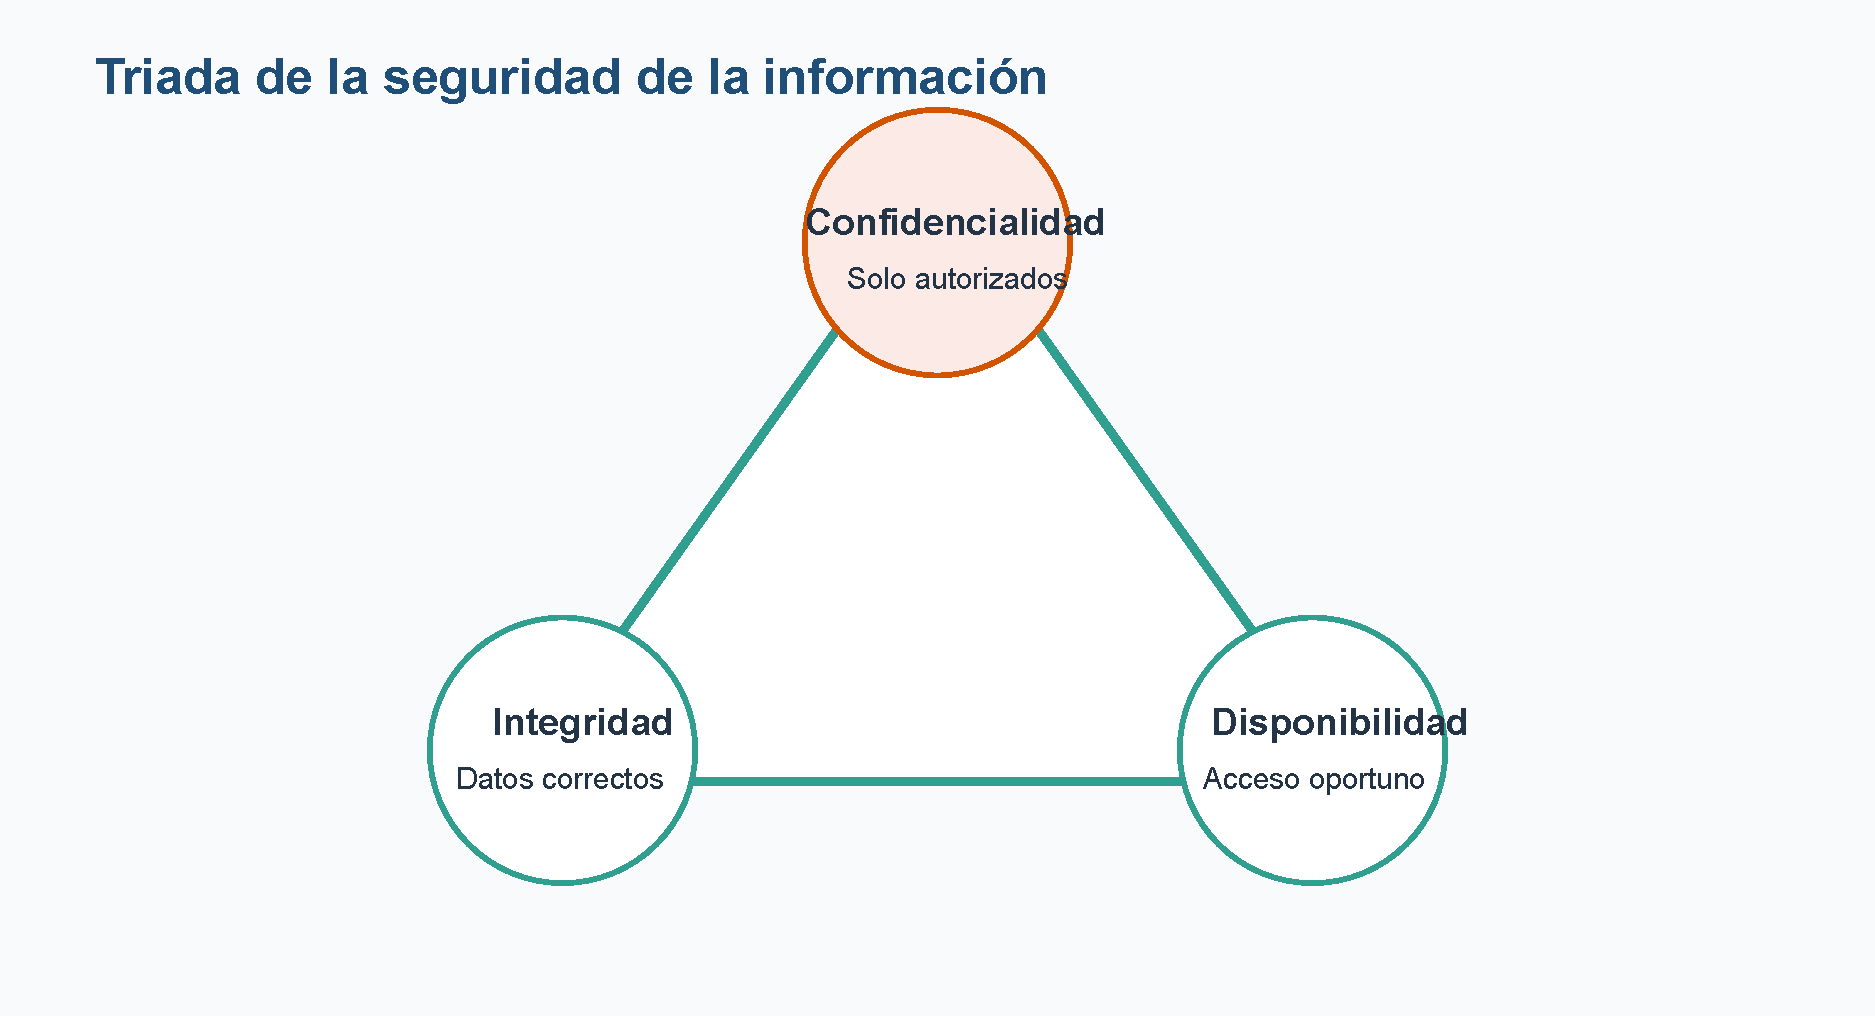
\includegraphics[width=0.78\linewidth,height=\textheight,keepaspectratio]{index_files/mediabag/capitulos/img/clase_03/fig_03_08_cia.pdf}

}

\caption{\label{fig-cia}Triada de seguridad}

\end{figure}%

\section{Confidencialidad}\label{confidencialidad}

La información solo debe ser accesible para personas autorizadas.

Ejemplo: un estudiante consulta sus propias calificaciones, no las de
todo el grupo.

\section{Integridad}\label{integridad}

La información debe mantenerse correcta y solo modificarse mediante
procesos autorizados.

Ejemplo: el docente registra una nota y el estudiante únicamente la
consulta.

\section{Disponibilidad}\label{disponibilidad}

Los servicios deben estar accesibles cuando se necesitan.

Ejemplo: la plataforma de inscripción debe funcionar durante el período
de asignación de cursos.

\bookmarksetup{startatroot}

\chapter{Contraseñas y autenticación
multifactor}\label{contraseuxf1as-y-autenticaciuxf3n-multifactor}

Una contraseña segura debe ser difícil de adivinar y no reutilizarse en
múltiples servicios.

Buenas prácticas:

\begin{itemize}
\tightlist
\item
  Utilizar frases largas.
\item
  Evitar información personal.
\item
  No compartir credenciales.
\item
  Utilizar un gestor de contraseñas cuando sea permitido.
\item
  Activar autenticación multifactor.
\item
  Bloquear intentos repetidos.
\item
  Deshabilitar cuentas que ya no se utilizan.
\end{itemize}

\bookmarksetup{startatroot}

\chapter{Actualizaciones}\label{actualizaciones}

Los fabricantes publican correcciones para errores y vulnerabilidades.

Un proceso responsable incluye:

\begin{enumerate}
\def\labelenumi{\arabic{enumi}.}
\tightlist
\item
  Identificar actualizaciones.
\item
  Revisar su impacto.
\item
  Probarlas.
\item
  Programar una ventana de mantenimiento.
\item
  Aplicarlas.
\item
  Verificar los servicios.
\item
  Documentar el resultado.
\end{enumerate}

\bookmarksetup{startatroot}

\chapter{Copias de seguridad}\label{copias-de-seguridad}

Un respaldo es una copia diseñada para recuperar información después de
una falla, error o incidente.

\section{Regla 3-2-1}\label{regla-3-2-1}

\begin{itemize}
\tightlist
\item
  Mantener tres copias de la información.
\item
  Utilizar dos medios diferentes.
\item
  Conservar una copia fuera del sitio principal.
\end{itemize}

\section{Un respaldo debe probarse}\label{un-respaldo-debe-probarse}

No basta con que el sistema indique ``copia finalizada''. Es necesario
verificar que los archivos puedan recuperarse.

\begin{tcolorbox}[enhanced jigsaw, arc=.35mm, bottomrule=.15mm, breakable, colback=white, colframe=quarto-callout-warning-color-frame, left=2mm, leftrule=.75mm, opacityback=0, rightrule=.15mm, toprule=.15mm]
\begin{minipage}[t]{5.5mm}
\textcolor{quarto-callout-warning-color}{\faExclamationTriangle}
\end{minipage}%
\begin{minipage}[t]{\textwidth - 5.5mm}

\vspace{-3mm}\textbf{Advertencia}\vspace{3mm}

Un respaldo que nunca ha sido restaurado es una promesa, no una
garantía.

\end{minipage}%
\end{tcolorbox}

\bookmarksetup{startatroot}

\chapter{Registros y auditoría}\label{registros-y-auditoruxeda}

Los servidores generan registros o \emph{logs}.

Pueden indicar:

\begin{itemize}
\tightlist
\item
  Inicios de sesión.
\item
  Intentos fallidos.
\item
  Cambios de configuración.
\item
  Errores.
\item
  Accesos a recursos.
\item
  Inicio y detención de servicios.
\end{itemize}

La auditoría permite investigar incidentes y demostrar el cumplimiento
de políticas.

\bookmarksetup{startatroot}

\chapter{Seguridad física}\label{seguridad-fuxedsica}

También deben protegerse:

\begin{itemize}
\tightlist
\item
  El acceso al cuarto de servidores.
\item
  La energía eléctrica.
\item
  La temperatura.
\item
  La humedad.
\item
  El riesgo de incendio.
\item
  La conectividad.
\item
  Los dispositivos de almacenamiento.
\end{itemize}

Un servidor protegido con contraseñas no está seguro si cualquier
persona puede desconectarlo o retirar sus discos.

\bookmarksetup{startatroot}

\chapter{Continuidad operativa}\label{continuidad-operativa}

La continuidad busca que la organización pueda seguir funcionando o
recuperarse en un tiempo aceptable.

Incluye:

\begin{itemize}
\tightlist
\item
  Redundancia.
\item
  Respaldos.
\item
  Planes de recuperación.
\item
  Documentación.
\item
  Contactos de emergencia.
\item
  Pruebas.
\item
  Responsables claramente definidos.
\end{itemize}

\bookmarksetup{startatroot}

\chapter{Ingeniería en la vida
real}\label{ingenieruxeda-en-la-vida-real-1}

Supongamos que una universidad tiene un único servidor que proporciona
autenticación, DNS, DHCP, archivos y el Campus Virtual.

Si ese servidor falla:

\begin{itemize}
\tightlist
\item
  Los usuarios no pueden iniciar sesión.
\item
  Los equipos nuevos no reciben IP.
\item
  Los nombres no se resuelven.
\item
  Las carpetas desaparecen.
\item
  La plataforma deja de funcionar.
\end{itemize}

El problema no es únicamente técnico. Puede detener clases, evaluaciones
y procesos administrativos.

Un ingeniero debe anticipar:

\begin{itemize}
\tightlist
\item
  ¿Qué servicios son críticos?
\item
  ¿Cuánto tiempo pueden estar fuera de línea?
\item
  ¿Qué datos deben recuperarse?
\item
  ¿Existe un servidor alterno?
\item
  ¿Quién tomará decisiones durante el incidente?
\end{itemize}

\bookmarksetup{startatroot}

\chapter{Verifica tu comprensión}\label{verifica-tu-comprensiuxf3n}

\section{Pregunta 1}\label{pregunta-1}

¿Cuál es la diferencia principal entre una arquitectura Punto a Punto y
una Cliente/Servidor?

\begin{enumerate}
\def\labelenumi{\alph{enumi}.}
\tightlist
\item
  El tipo de cable utilizado.\\
\item
  La existencia de administración y servicios centralizados.\\
\item
  La marca de las computadoras.\\
\item
  La velocidad de Internet.
\end{enumerate}

\section{Pregunta 2}\label{pregunta-2}

¿Qué servicio traduce nombres de dominio en direcciones IP?

\begin{enumerate}
\def\labelenumi{\alph{enumi}.}
\tightlist
\item
  DHCP.\\
\item
  DNS.\\
\item
  SMB.\\
\item
  SSH.
\end{enumerate}

\section{Pregunta 3}\label{pregunta-3}

¿Qué servicio asigna automáticamente direcciones IP?

\begin{enumerate}
\def\labelenumi{\alph{enumi}.}
\tightlist
\item
  DNS.\\
\item
  HTTP.\\
\item
  DHCP.\\
\item
  LDAP.
\end{enumerate}

\section{Pregunta 4}\label{pregunta-4}

¿Qué elemento facilita asignar permisos a muchas personas con funciones
semejantes?

\begin{enumerate}
\def\labelenumi{\alph{enumi}.}
\tightlist
\item
  Un grupo.\\
\item
  Una impresora.\\
\item
  Una dirección IP.\\
\item
  Un navegador.
\end{enumerate}

\section{Pregunta 5}\label{pregunta-5}

¿Cuál es un ejemplo del principio del mínimo privilegio?

\begin{enumerate}
\def\labelenumi{\alph{enumi}.}
\tightlist
\item
  Todos son administradores.\\
\item
  Cada usuario recibe únicamente el acceso necesario.\\
\item
  Se comparte una sola cuenta.\\
\item
  Se desactiva la auditoría.
\end{enumerate}

\section{Pregunta 6}\label{pregunta-6}

¿Qué objetivo de seguridad se relaciona con mantener un servicio
accesible?

\begin{enumerate}
\def\labelenumi{\alph{enumi}.}
\tightlist
\item
  Confidencialidad.\\
\item
  Integridad.\\
\item
  Disponibilidad.\\
\item
  Portabilidad.
\end{enumerate}

\begin{tcolorbox}[enhanced jigsaw, arc=.35mm, bottomrule=.15mm, breakable, colback=white, colframe=quarto-callout-note-color-frame, left=2mm, leftrule=.75mm, opacityback=0, rightrule=.15mm, toprule=.15mm]
\begin{minipage}[t]{5.5mm}
\textcolor{quarto-callout-note-color}{\faInfo}
\end{minipage}%
\begin{minipage}[t]{\textwidth - 5.5mm}

\vspace{-3mm}\textbf{Respuestas}\vspace{3mm}

\begin{enumerate}
\def\labelenumi{\arabic{enumi}.}
\tightlist
\item
  b\\
\item
  b\\
\item
  c\\
\item
  a\\
\item
  b\\
\item
  c
\end{enumerate}

\end{minipage}%
\end{tcolorbox}

\bookmarksetup{startatroot}

\chapter{Laboratorio narrativo: diseñando la red de una
academia}\label{laboratorio-narrativo-diseuxf1ando-la-red-de-una-academia}

\section{Situación}\label{situaciuxf3n-1}

La Academia Horizonte abrirá una nueva sede.

Contará con:

\begin{itemize}
\tightlist
\item
  28 computadoras para estudiantes.
\item
  4 computadoras administrativas.
\item
  3 computadoras para docentes.
\item
  2 impresoras.
\item
  Una conexión a Internet.
\item
  Una plataforma académica.
\item
  Documentos financieros.
\item
  Materiales de clase compartidos.
\end{itemize}

Actualmente, cada computadora utiliza cuentas locales y los archivos se
transfieren mediante memorias USB.

La dirección solicita una propuesta básica de red.

\section{Misión}\label{misiuxf3n}

Actúe como integrante del equipo de infraestructura y diseñe una
solución inicial.

\section{Parte 1. Arquitectura}\label{parte-1.-arquitectura}

Responda:

\begin{enumerate}
\def\labelenumi{\arabic{enumi}.}
\tightlist
\item
  ¿Implementaría Punto a Punto o Cliente/Servidor?
\item
  Justifique la decisión con al menos tres criterios.
\item
  ¿Qué riesgos tendría mantener cuentas locales independientes?
\end{enumerate}

\section{Parte 2. Roles}\label{parte-2.-roles}

Seleccione los roles necesarios.

{\def\LTcaptype{none} % do not increment counter
\begin{longtable}[]{@{}lll@{}}
\toprule\noalign{}
Rol & ¿Se necesita? & Justificación \\
\midrule\noalign{}
\endhead
\bottomrule\noalign{}
\endlastfoot
DNS & & \\
DHCP & & \\
Directorio & & \\
Archivos & & \\
Impresión & & \\
Web & & \\
Base de datos & & \\
Respaldo & & \\
Monitoreo & & \\
\end{longtable}
}

\section{Parte 3. Usuarios y grupos}\label{parte-3.-usuarios-y-grupos}

Proponga grupos.

Ejemplo:

\begin{itemize}
\tightlist
\item
  Administrativos.
\item
  Docentes.
\item
  Estudiantes.
\item
  Soporte Técnico.
\end{itemize}

Indique qué recursos debe utilizar cada grupo.

\section{Parte 4. Permisos}\label{parte-4.-permisos}

Diseñe una matriz.

{\def\LTcaptype{none} % do not increment counter
\begin{longtable}[]{@{}lllll@{}}
\toprule\noalign{}
Recurso & Administrativos & Docentes & Estudiantes & Soporte \\
\midrule\noalign{}
\endhead
\bottomrule\noalign{}
\endlastfoot
Finanzas & & & & \\
Materiales docentes & & & & \\
Entregas estudiantiles & & & & \\
Configuración de servidores & & & & \\
Impresoras & & & & \\
\end{longtable}
}

Utilice valores como:

\begin{itemize}
\tightlist
\item
  Sin acceso.
\item
  Lectura.
\item
  Lectura y escritura.
\item
  Administración.
\end{itemize}

\section{Parte 5. Seguridad}\label{parte-5.-seguridad}

Proponga al menos una medida para cada categoría:

\begin{itemize}
\tightlist
\item
  Contraseñas.
\item
  Respaldos.
\item
  Actualizaciones.
\item
  Auditoría.
\item
  Seguridad física.
\item
  Continuidad.
\end{itemize}

\section{Parte 6. Diagrama}\label{parte-6.-diagrama}

Dibuje la infraestructura propuesta.

Debe incluir:

\begin{itemize}
\tightlist
\item
  Internet.
\item
  Firewall o router.
\item
  Servidor o servidores.
\item
  Switch.
\item
  Computadoras.
\item
  Impresoras.
\item
  Respaldos.
\end{itemize}

\section{Producto esperado}\label{producto-esperado}

Entregue:

\begin{enumerate}
\def\labelenumi{\arabic{enumi}.}
\tightlist
\item
  Una justificación de la arquitectura.
\item
  La lista de roles.
\item
  Los grupos.
\item
  La matriz de permisos.
\item
  Las medidas de seguridad.
\item
  El diagrama.
\end{enumerate}

\bookmarksetup{startatroot}

\chapter{Reto del Ingeniero}\label{reto-del-ingeniero}

Una clínica pequeña posee diez computadoras. El expediente de pacientes
se almacena en una carpeta compartida desde la computadora de recepción.

La recepcionista apaga su equipo al finalizar la jornada y, durante ese
tiempo, nadie puede consultar los expedientes. Todos conocen la misma
contraseña y no existen respaldos.

Responda:

\begin{enumerate}
\def\labelenumi{\arabic{enumi}.}
\tightlist
\item
  Identifique cinco riesgos.
\item
  Proponga una arquitectura mejor.
\item
  Defina tres grupos de usuarios.
\item
  Asigne permisos generales.
\item
  Indique qué servicios implementaría.
\item
  Diseñe una estrategia básica de respaldo.
\item
  Explique cómo mejoraría la disponibilidad.
\end{enumerate}

\bookmarksetup{startatroot}

\chapter{Resumen de la clase}\label{resumen-de-la-clase-2}

En esta clase aprendimos que:

\begin{itemize}
\tightlist
\item
  Un Sistema Operativo de Red administra recursos compartidos.
\item
  La arquitectura Punto a Punto es sencilla, pero posee limitaciones.
\item
  Cliente/Servidor permite centralizar servicios y crecer.
\item
  DNS traduce nombres en direcciones IP.
\item
  DHCP entrega automáticamente la configuración de red.
\item
  Los usuarios representan identidades.
\item
  Los grupos facilitan la administración.
\item
  Los permisos controlan acciones.
\item
  Un servidor puede desempeñar diferentes roles.
\item
  Windows Server, Linux y UNIX ofrecen soluciones distintas.
\item
  La seguridad debe proteger confidencialidad, integridad y
  disponibilidad.
\item
  Los respaldos, actualizaciones, registros y controles físicos son
  esenciales.
\item
  Una infraestructura debe diseñarse según necesidades reales.
\end{itemize}

\begin{tcolorbox}[enhanced jigsaw, arc=.35mm, bottomrule=.15mm, breakable, colback=white, colframe=quarto-callout-tip-color-frame, left=2mm, leftrule=.75mm, opacityback=0, rightrule=.15mm, toprule=.15mm]
\begin{minipage}[t]{5.5mm}
\textcolor{quarto-callout-tip-color}{\faLightbulb}
\end{minipage}%
\begin{minipage}[t]{\textwidth - 5.5mm}

\vspace{-3mm}\textbf{Lo esencial que debes recordar}\vspace{3mm}

Si puedes explicar con tus propias palabras cómo un usuario obtiene una
dirección IP, localiza un servidor, inicia sesión y accede únicamente a
los recursos autorizados, habrás comprendido la idea central de esta
clase.

\end{minipage}%
\end{tcolorbox}

\bookmarksetup{startatroot}

\chapter{Cierre de la clase}\label{cierre-de-la-clase}

Un Sistema Operativo de Red convierte un conjunto de computadoras en una
infraestructura organizada.

La tecnología visible para el usuario puede ser una pantalla de inicio
de sesión o una carpeta compartida. Sin embargo, detrás de esa
simplicidad existen decisiones de arquitectura, servicios, seguridad y
continuidad.

El trabajo del ingeniero consiste en lograr que todos esos componentes
funcionen como un sistema confiable.

\bookmarksetup{startatroot}

\chapter{Referencias}\label{referencias}

\begin{itemize}
\tightlist
\item
  Kurose, J. F., \& Ross, K. W. \emph{Computer Networking: A Top-Down
  Approach}. Pearson.
\item
  Nemeth, E., Snyder, G., Hein, T. R., Whaley, B., \& Mackin, D.
  \emph{UNIX and Linux System Administration Handbook}. Addison-Wesley.
\item
  Silberschatz, A., Galvin, P. B., \& Gagne, G. \emph{Operating System
  Concepts}. Wiley.
\item
  Stallings, W. \emph{Operating Systems: Internals and Design
  Principles}. Pearson.
\item
  Tanenbaum, A. S., \& Bos, H. \emph{Modern Operating Systems}. Pearson.
\item
  Documentación técnica de Microsoft Learn sobre Windows Server y
  servicios de red.
\item
  Documentación técnica de Red Hat sobre administración de sistemas
  Linux.
\end{itemize}

\bookmarksetup{startatroot}

\chapter{Clase 4. Administración de
Procesos}\label{clase-4.-administraciuxf3n-de-procesos}

\bookmarksetup{startatroot}

\chapter{Presentación}\label{presentaciuxf3n}

Cada vez que abrimos un navegador, reproducimos música o editamos un
documento, el Sistema Operativo crea y administra procesos. Aunque
parezca que todas las aplicaciones trabajan al mismo tiempo, en realidad
el procesador distribuye su tiempo entre ellas de forma extremadamente
rápida.

\begin{tcolorbox}[enhanced jigsaw, arc=.35mm, bottomrule=.15mm, bottomtitle=1mm, breakable, colback=white, colbacktitle=quarto-callout-tip-color!10!white, colframe=quarto-callout-tip-color-frame, coltitle=black, left=2mm, leftrule=.75mm, opacityback=0, opacitybacktitle=0.6, rightrule=.15mm, title=\textcolor{quarto-callout-tip-color}{\faLightbulb}\hspace{0.5em}{Objetivos}, titlerule=0mm, toprule=.15mm, toptitle=1mm]

\begin{itemize}
\tightlist
\item
  Comprender qué es un proceso.
\item
  Diferenciar programa y proceso.
\item
  Explicar el modelo de procesos.
\item
  Comprender los estados de un proceso.
\item
  Interpretar el funcionamiento del PCB.
\end{itemize}

\end{tcolorbox}

\bookmarksetup{startatroot}

\chapter{¿Qué es un proceso?}\label{quuxe9-es-un-proceso}

Un \textbf{proceso} es un programa que se encuentra en ejecución junto
con todos los recursos que necesita para funcionar: memoria, registros,
archivos abiertos y tiempo de CPU.

{\def\LTcaptype{none} % do not increment counter
\begin{longtable}[]{@{}ll@{}}
\toprule\noalign{}
Programa & Proceso \\
\midrule\noalign{}
\endhead
\bottomrule\noalign{}
\endlastfoot
Archivo almacenado & Programa en ejecución \\
Pasivo & Dinámico \\
No consume recursos & Consume CPU, memoria y E/S \\
\end{longtable}
}

\section{Analogía}\label{analoguxeda}

Una receta de cocina representa un \textbf{programa}. Preparar la receta
utilizando ingredientes, tiempo y utensilios representa el
\textbf{proceso}.

\bookmarksetup{startatroot}

\chapter{Modelo de Procesos}\label{modelo-de-procesos}

El Sistema Operativo crea la ilusión de que cada aplicación posee su
propio procesador. En realidad, el \textbf{Scheduler} distribuye
pequeños intervalos de tiempo entre todos los procesos.

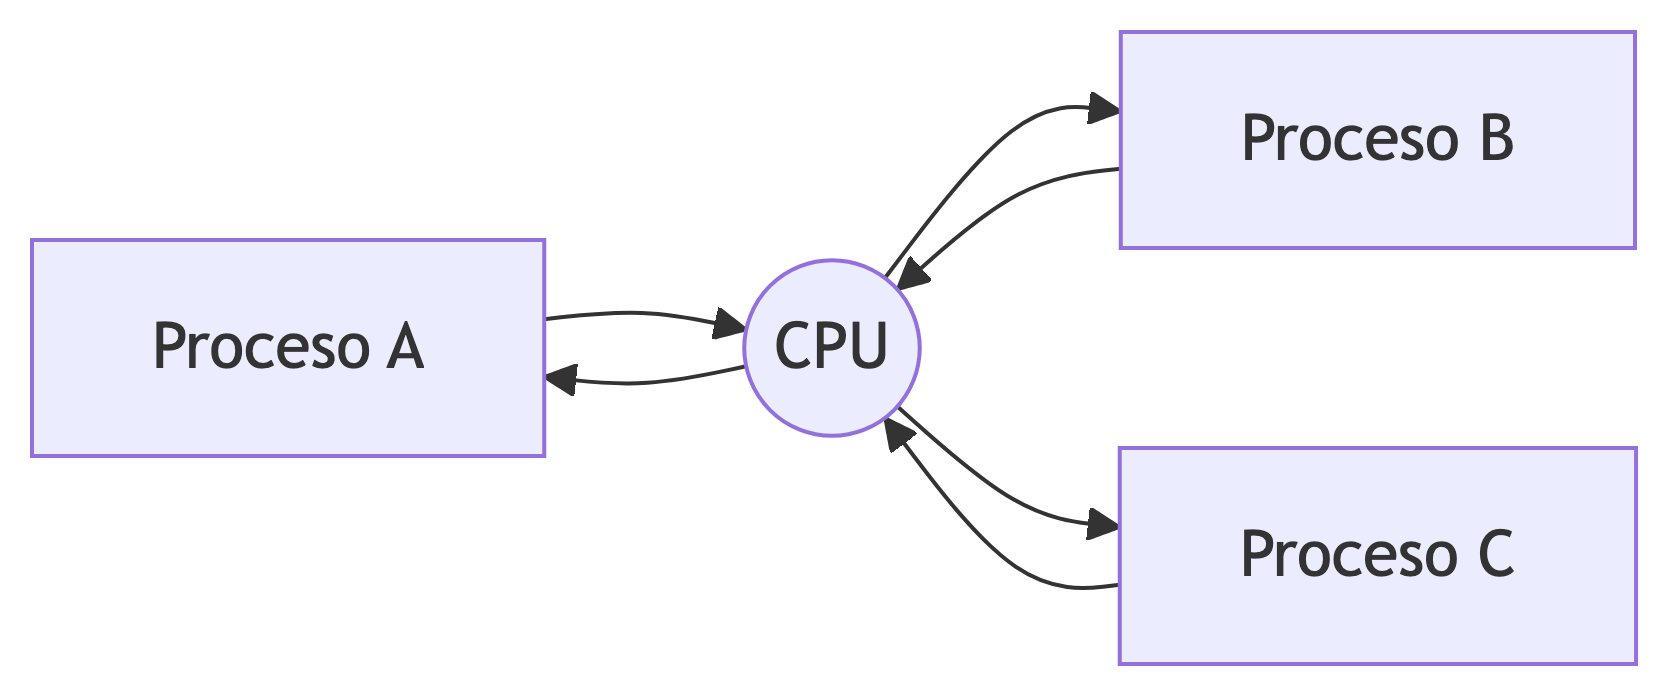
\includegraphics[width=4.34in,height=1.81in]{capitulos/04_administracion_procesos_files/figure-latex/mermaid-figure-1.png}

\begin{tcolorbox}[enhanced jigsaw, arc=.35mm, bottomrule=.15mm, bottomtitle=1mm, breakable, colback=white, colbacktitle=quarto-callout-note-color!10!white, colframe=quarto-callout-note-color-frame, coltitle=black, left=2mm, leftrule=.75mm, opacityback=0, opacitybacktitle=0.6, rightrule=.15mm, title=\textcolor{quarto-callout-note-color}{\faInfo}\hspace{0.5em}{Idea clave}, titlerule=0mm, toprule=.15mm, toptitle=1mm]

La multitarea es posible porque el Sistema Operativo cambia rápidamente
entre procesos mediante el \textbf{Cambio de Contexto (Context Switch)}.

\end{tcolorbox}

\bookmarksetup{startatroot}

\chapter{Programa vs.~Proceso}\label{programa-vs.-proceso}

Un único programa puede generar múltiples procesos independientes.

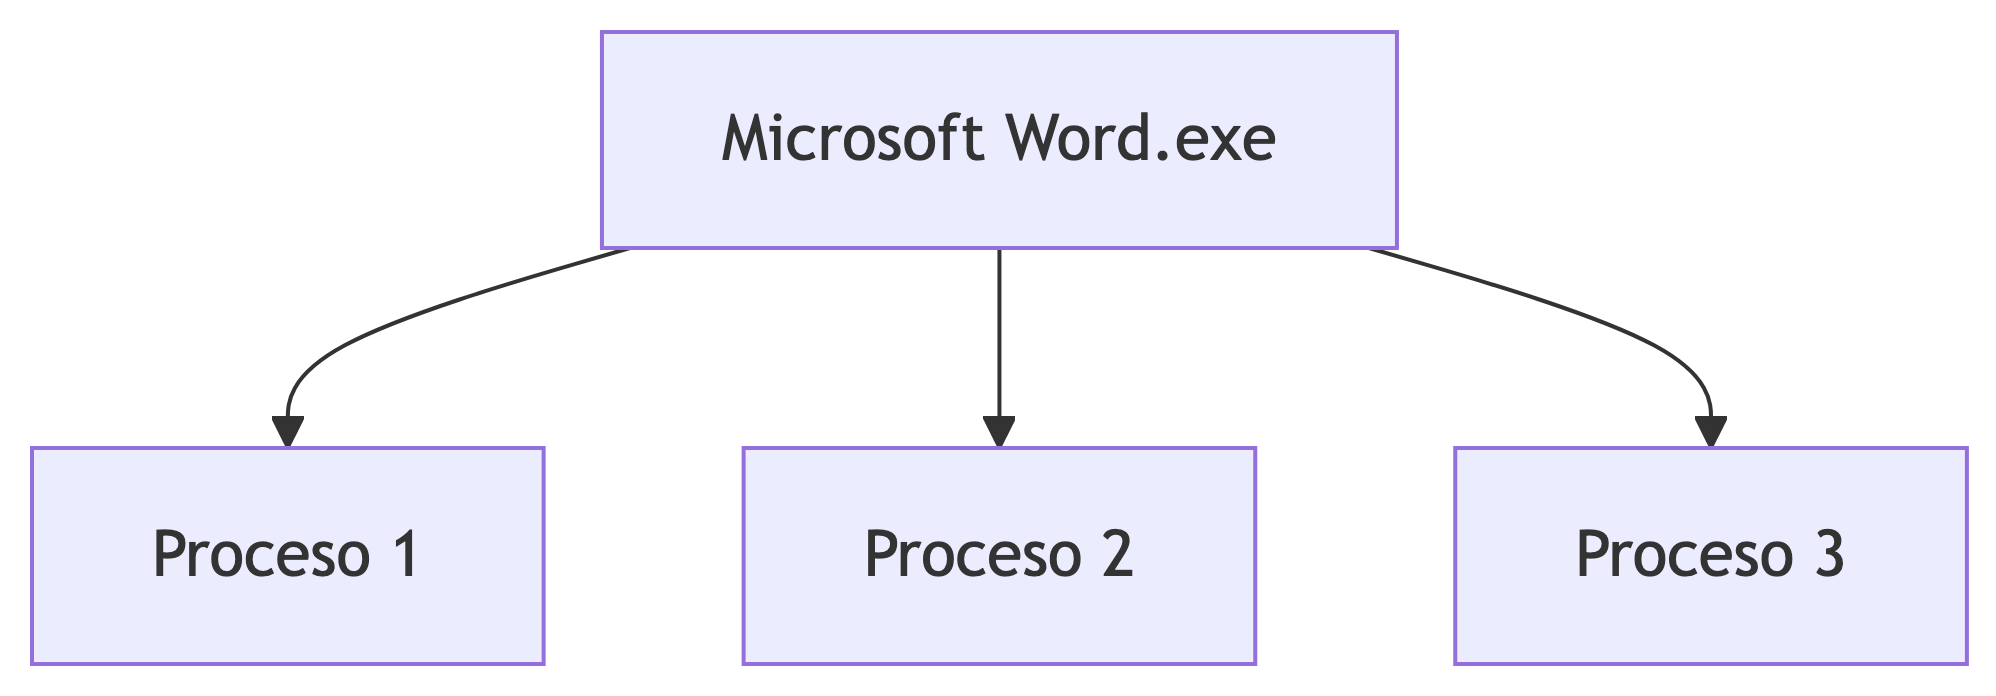
\includegraphics[width=5.21in,height=1.81in]{capitulos/04_administracion_procesos_files/figure-latex/mermaid-figure-10.png}

\bookmarksetup{startatroot}

\chapter{Espacio de Direcciones}\label{espacio-de-direcciones}

Cada proceso dispone de un espacio de memoria independiente.

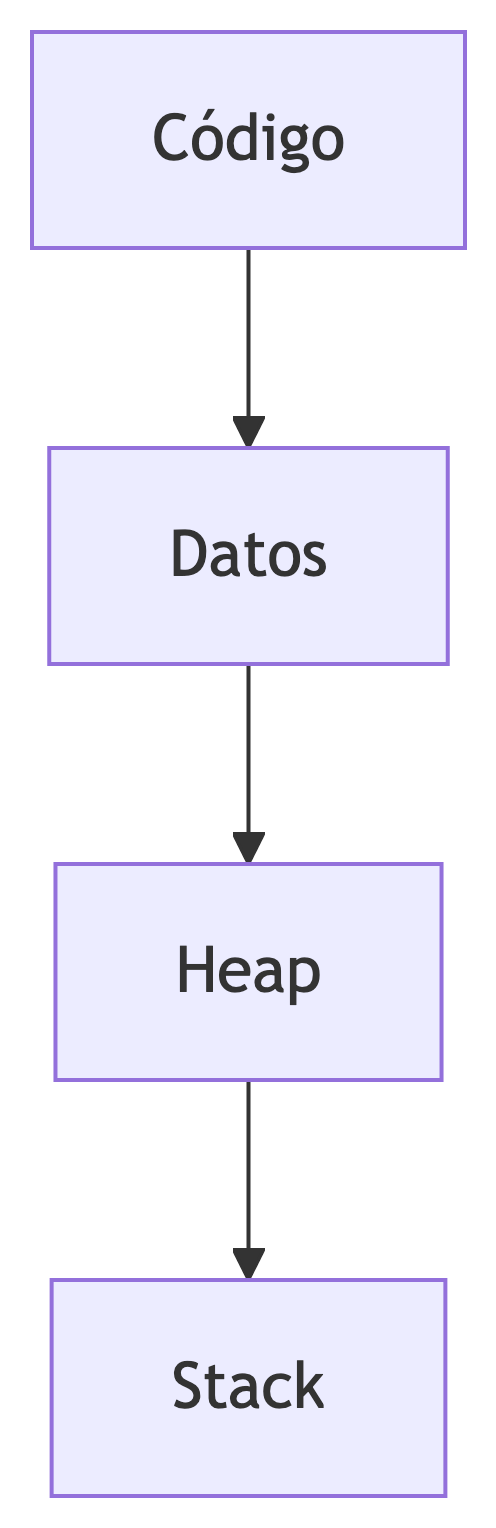
\includegraphics[width=1.29in,height=3.98in]{capitulos/04_administracion_procesos_files/figure-latex/mermaid-figure-9.png}

\bookmarksetup{startatroot}

\chapter{Bloque de Control del Proceso
(PCB)}\label{bloque-de-control-del-proceso-pcb}

El PCB es el expediente administrativo del proceso.

{\def\LTcaptype{none} % do not increment counter
\begin{longtable}[]{@{}ll@{}}
\toprule\noalign{}
Campo & Descripción \\
\midrule\noalign{}
\endhead
\bottomrule\noalign{}
\endlastfoot
PID & Identificador único \\
Estado & Estado actual \\
Program Counter & Próxima instrucción \\
Registros & Contexto de CPU \\
Memoria & Espacio asignado \\
Archivos & Recursos abiertos \\
\end{longtable}
}

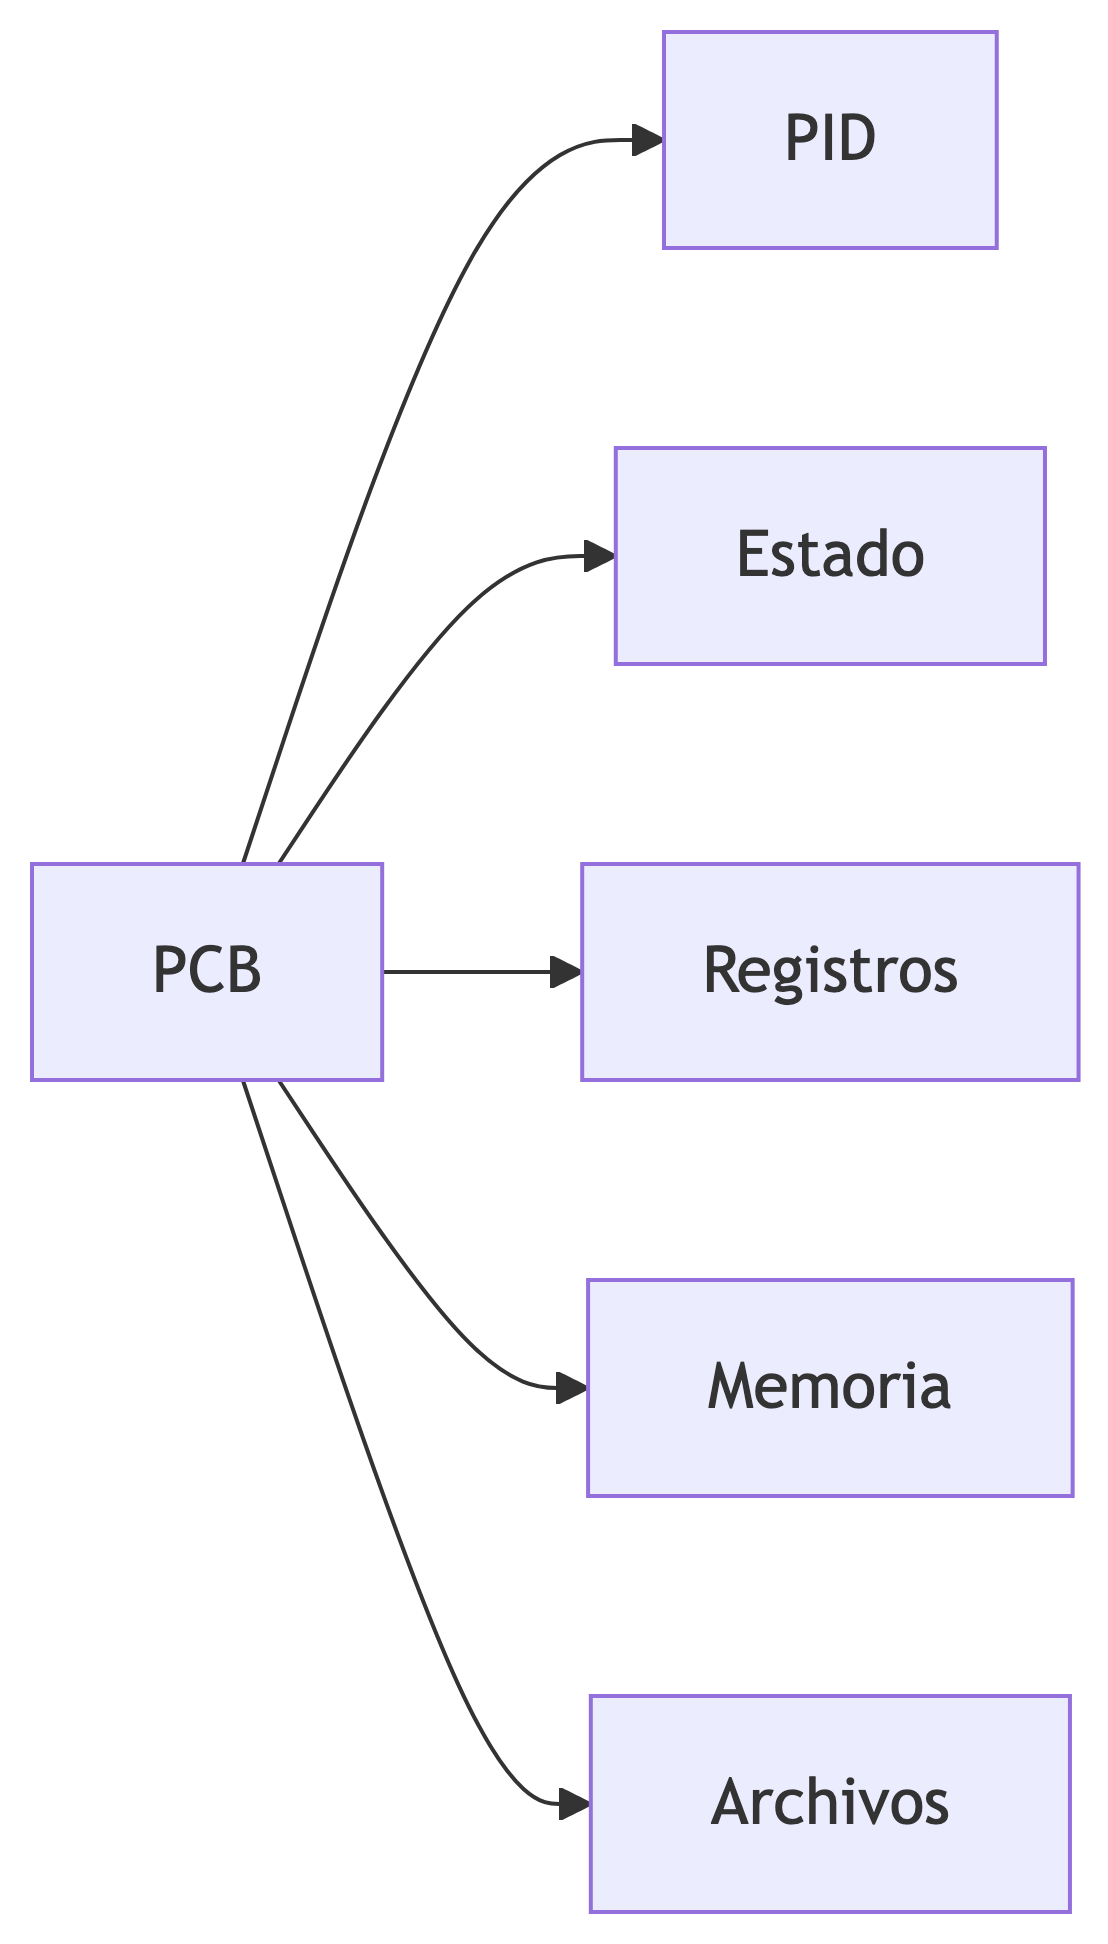
\includegraphics[width=2.89in,height=5.06in]{capitulos/04_administracion_procesos_files/figure-latex/mermaid-figure-8.png}

\bookmarksetup{startatroot}

\chapter{Tabla de Procesos}\label{tabla-de-procesos}

El kernel mantiene una tabla donde registra todos los PCB existentes.

\begin{tcolorbox}[enhanced jigsaw, arc=.35mm, bottomrule=.15mm, bottomtitle=1mm, breakable, colback=white, colbacktitle=quarto-callout-tip-color!10!white, colframe=quarto-callout-tip-color-frame, coltitle=black, left=2mm, leftrule=.75mm, opacityback=0, opacitybacktitle=0.6, rightrule=.15mm, title=\textcolor{quarto-callout-tip-color}{\faLightbulb}\hspace{0.5em}{Estructura simplificada de una Tabla de Procesos}, titlerule=0mm, toprule=.15mm, toptitle=1mm]

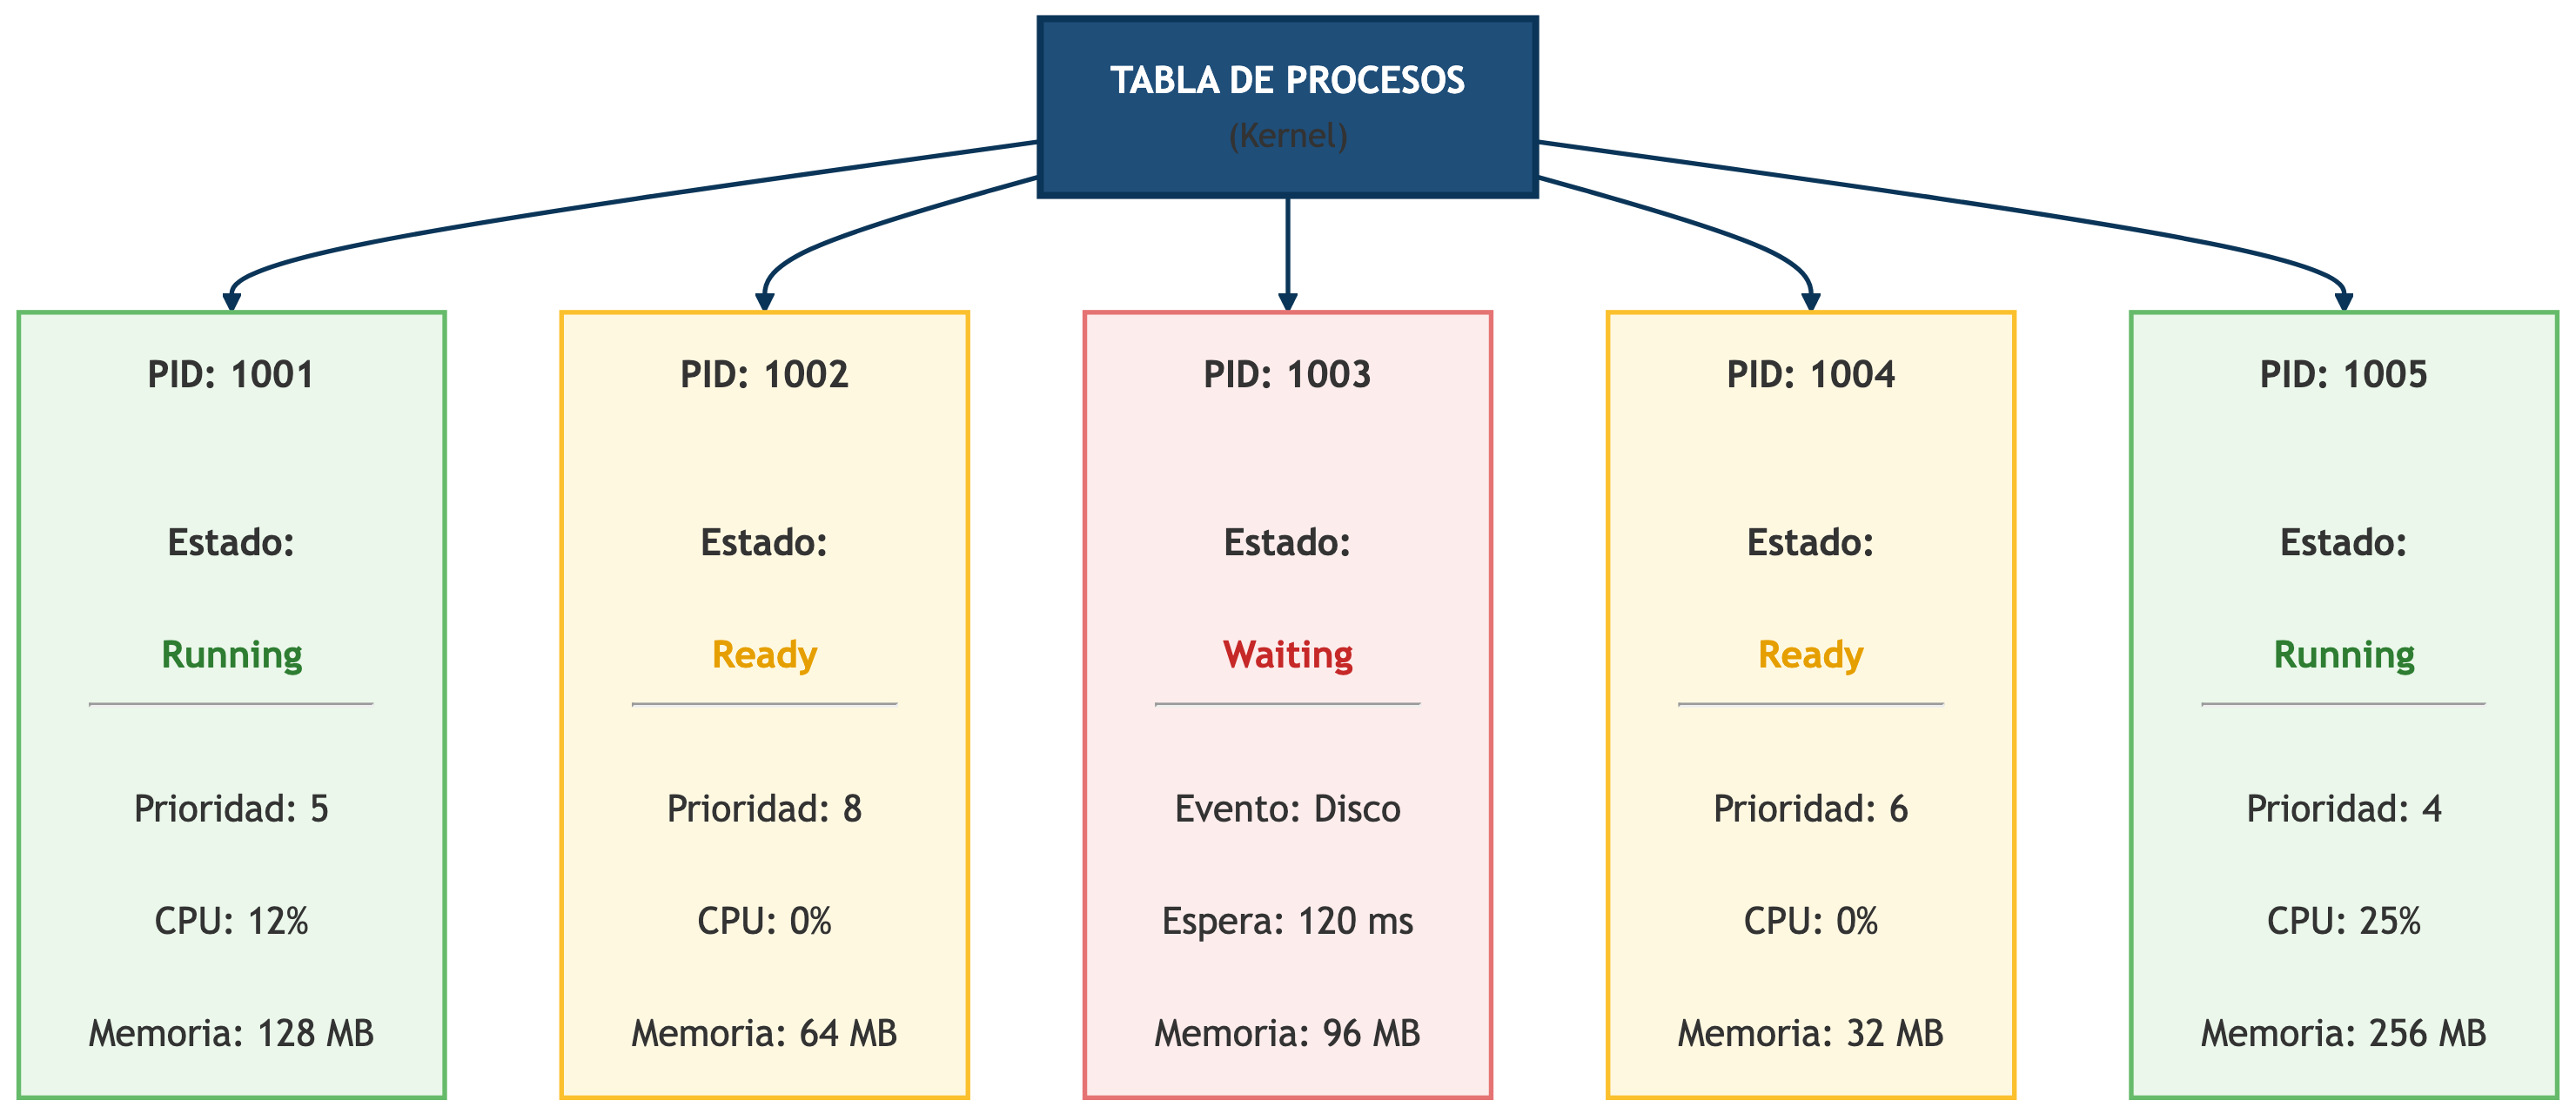
\includegraphics[width=11.48in,height=4.98in]{capitulos/04_administracion_procesos_files/figure-latex/mermaid-figure-7.png}

La tabla de procesos es una estructura interna mantenida por el
\textbf{Kernel}, donde se almacena el \textbf{PCB (Process Control
Block)} de todos los procesos existentes en el sistema. Cada entrada
contiene la información necesaria para que el sistema operativo pueda
administrar correctamente cada proceso.

\end{tcolorbox}

\subsection{Ejemplo de una Tabla de
Procesos}\label{ejemplo-de-una-tabla-de-procesos}

{\def\LTcaptype{none} % do not increment counter
\begin{longtable}[]{@{}
  >{\centering\arraybackslash}p{(\linewidth - 12\tabcolsep) * \real{0.0575}}
  >{\raggedright\arraybackslash}p{(\linewidth - 12\tabcolsep) * \real{0.2299}}
  >{\centering\arraybackslash}p{(\linewidth - 12\tabcolsep) * \real{0.1034}}
  >{\centering\arraybackslash}p{(\linewidth - 12\tabcolsep) * \real{0.1264}}
  >{\raggedleft\arraybackslash}p{(\linewidth - 12\tabcolsep) * \real{0.1609}}
  >{\raggedleft\arraybackslash}p{(\linewidth - 12\tabcolsep) * \real{0.1034}}
  >{\raggedleft\arraybackslash}p{(\linewidth - 12\tabcolsep) * \real{0.2184}}@{}}
\toprule\noalign{}
\begin{minipage}[b]{\linewidth}\centering
PID
\end{minipage} & \begin{minipage}[b]{\linewidth}\raggedright
Nombre del proceso
\end{minipage} & \begin{minipage}[b]{\linewidth}\centering
Estado
\end{minipage} & \begin{minipage}[b]{\linewidth}\centering
Prioridad
\end{minipage} & \begin{minipage}[b]{\linewidth}\raggedleft
Memoria (MB)
\end{minipage} & \begin{minipage}[b]{\linewidth}\raggedleft
CPU (\%)
\end{minipage} & \begin{minipage}[b]{\linewidth}\raggedleft
Archivos abiertos
\end{minipage} \\
\midrule\noalign{}
\endhead
\bottomrule\noalign{}
\endlastfoot
1001 & Chrome.exe & Running & Alta & 245 & 18 & 27 \\
1002 & Word.exe & Ready & Media & 132 & 0 & 12 \\
1003 & Spotify.exe & Waiting & Baja & 95 & 0 & 8 \\
1004 & Teams.exe & Ready & Alta & 318 & 0 & 34 \\
1005 & Explorer.exe & Running & Alta & 76 & 5 & 19 \\
\end{longtable}
}

\textbf{Interpretación}

\begin{itemize}
\tightlist
\item
  \textbf{PID:} Identificador único asignado por el sistema operativo.
\item
  \textbf{Nombre del proceso:} Aplicación o servicio que se encuentra en
  ejecución.
\item
  \textbf{Estado:} Situación actual del proceso (Running, Ready o
  Waiting).
\item
  \textbf{Prioridad:} Nivel de importancia utilizado por el Scheduler.
\item
  \textbf{Memoria:} Cantidad de memoria RAM reservada por el proceso.
\item
  \textbf{CPU:} Porcentaje de utilización del procesador en ese
  instante.
\item
  \textbf{Archivos abiertos:} Número de archivos o recursos que el
  proceso mantiene abiertos.
\end{itemize}

\bookmarksetup{startatroot}

\chapter{Módelos de Estados de un
Proceso}\label{muxf3delos-de-estados-de-un-proceso}

\section{Evolución de los modelos de
estados}\label{evoluciuxf3n-de-los-modelos-de-estados}

{\def\LTcaptype{none} % do not increment counter
\begin{longtable}[]{@{}
  >{\raggedright\arraybackslash}p{(\linewidth - 4\tabcolsep) * \real{0.2368}}
  >{\raggedright\arraybackslash}p{(\linewidth - 4\tabcolsep) * \real{0.2368}}
  >{\raggedright\arraybackslash}p{(\linewidth - 4\tabcolsep) * \real{0.5263}}@{}}
\toprule\noalign{}
\begin{minipage}[b]{\linewidth}\raggedright
Modelo
\end{minipage} & \begin{minipage}[b]{\linewidth}\raggedright
Estados
\end{minipage} & \begin{minipage}[b]{\linewidth}\raggedright
¿Dónde se utiliza?
\end{minipage} \\
\midrule\noalign{}
\endhead
\bottomrule\noalign{}
\endlastfoot
Dos estados & Listo y Ejecución & Sistemas muy simples o con fines
didácticos. \\
Cinco estados & Nuevo, Listo, Ejecución, Bloqueado y Terminado & Es el
modelo más utilizado para explicar la administración de procesos. \\
Siete estados & Cinco estados + Listo Suspendido + Bloqueado Suspendido
& Sistemas operativos modernos que utilizan memoria virtual y Swap. \\
\end{longtable}
}

\section{Modelo de cinco estados}\label{modelo-de-cinco-estados}

El modelo de cinco estados es uno de los más utilizados para explicar el
ciclo de vida de un proceso en un sistema operativo. En este modelo, un
proceso puede encontrarse en uno de cinco estados bien definidos, y el
sistema operativo controla las transiciones entre ellos.

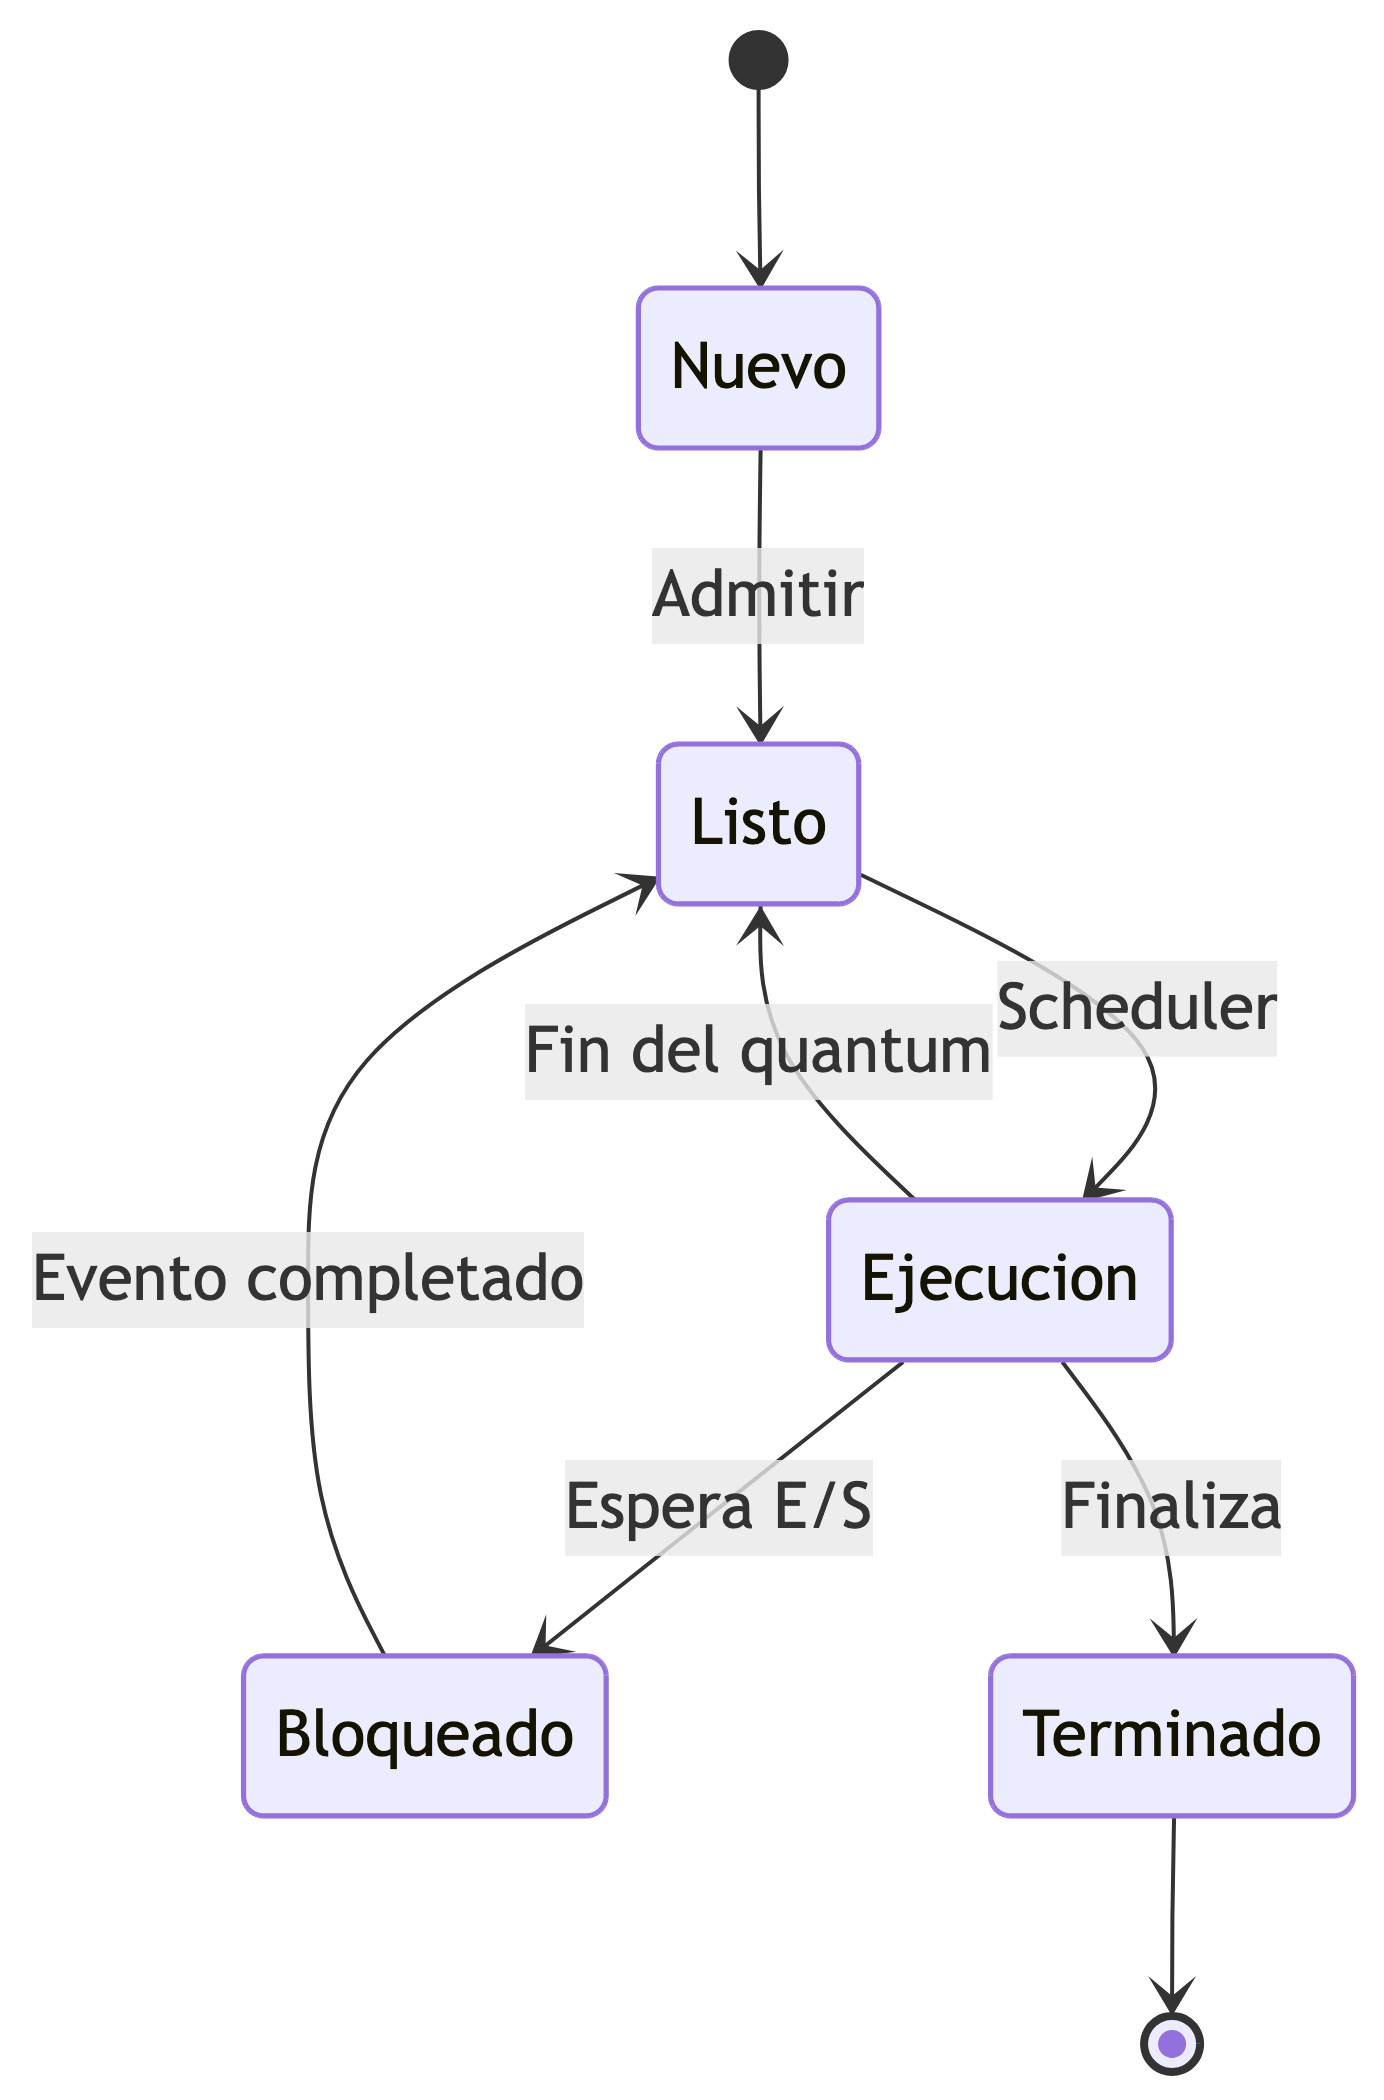
\includegraphics[width=3.61in,height=5.48in]{capitulos/04_administracion_procesos_files/figure-latex/mermaid-figure-6.png}

\subsection{Descripción de los
estados}\label{descripciuxf3n-de-los-estados}

{\def\LTcaptype{none} % do not increment counter
\begin{longtable}[]{@{}
  >{\raggedright\arraybackslash}p{(\linewidth - 2\tabcolsep) * \real{0.4091}}
  >{\raggedright\arraybackslash}p{(\linewidth - 2\tabcolsep) * \real{0.5909}}@{}}
\toprule\noalign{}
\begin{minipage}[b]{\linewidth}\raggedright
Estado
\end{minipage} & \begin{minipage}[b]{\linewidth}\raggedright
Descripción
\end{minipage} \\
\midrule\noalign{}
\endhead
\bottomrule\noalign{}
\endlastfoot
\textbf{Nuevo} & El proceso acaba de ser creado y aún no está listo para
ejecutarse. \\
\textbf{Listo (Ready)} & El proceso posee todos los recursos necesarios
excepto la CPU. Espera su turno para ejecutarse. \\
\textbf{Ejecución (Running)} & El proceso está utilizando el procesador
y ejecutando instrucciones. \\
\textbf{Bloqueado (Waiting)} & El proceso espera la finalización de una
operación de entrada/salida o algún evento externo. \\
\textbf{Terminado (Exit)} & El proceso concluyó su ejecución y el
sistema operativo libera los recursos utilizados. \\
\end{longtable}
}

\begin{tcolorbox}[enhanced jigsaw, arc=.35mm, bottomrule=.15mm, bottomtitle=1mm, breakable, colback=white, colbacktitle=quarto-callout-tip-color!10!white, colframe=quarto-callout-tip-color-frame, coltitle=black, left=2mm, leftrule=.75mm, opacityback=0, opacitybacktitle=0.6, rightrule=.15mm, title=\textcolor{quarto-callout-tip-color}{\faLightbulb}\hspace{0.5em}{Idea clave}, titlerule=0mm, toprule=.15mm, toptitle=1mm]

Todo proceso pasa necesariamente por los estados \textbf{Nuevo} y
\textbf{Terminado}, mientras que los estados \textbf{Listo},
\textbf{Ejecución} y \textbf{Bloqueado} pueden repetirse varias veces
durante su ciclo de vida.

\end{tcolorbox}

\section{Modelo con procesos suspendidos
(Swap)}\label{modelo-con-procesos-suspendidos-swap}

En sistemas multitarea es posible que la memoria principal no sea
suficiente para mantener todos los procesos cargados simultáneamente. En
estos casos, el sistema operativo puede mover temporalmente algunos
procesos al almacenamiento secundario mediante una técnica denominada
\textbf{Swap} o \textbf{Intercambio de memoria}.

Cuando esto ocurre aparecen dos nuevos estados:

\begin{itemize}
\tightlist
\item
  \textbf{Listo y Suspendido}
\item
  \textbf{Bloqueado y Suspendido}
\end{itemize}

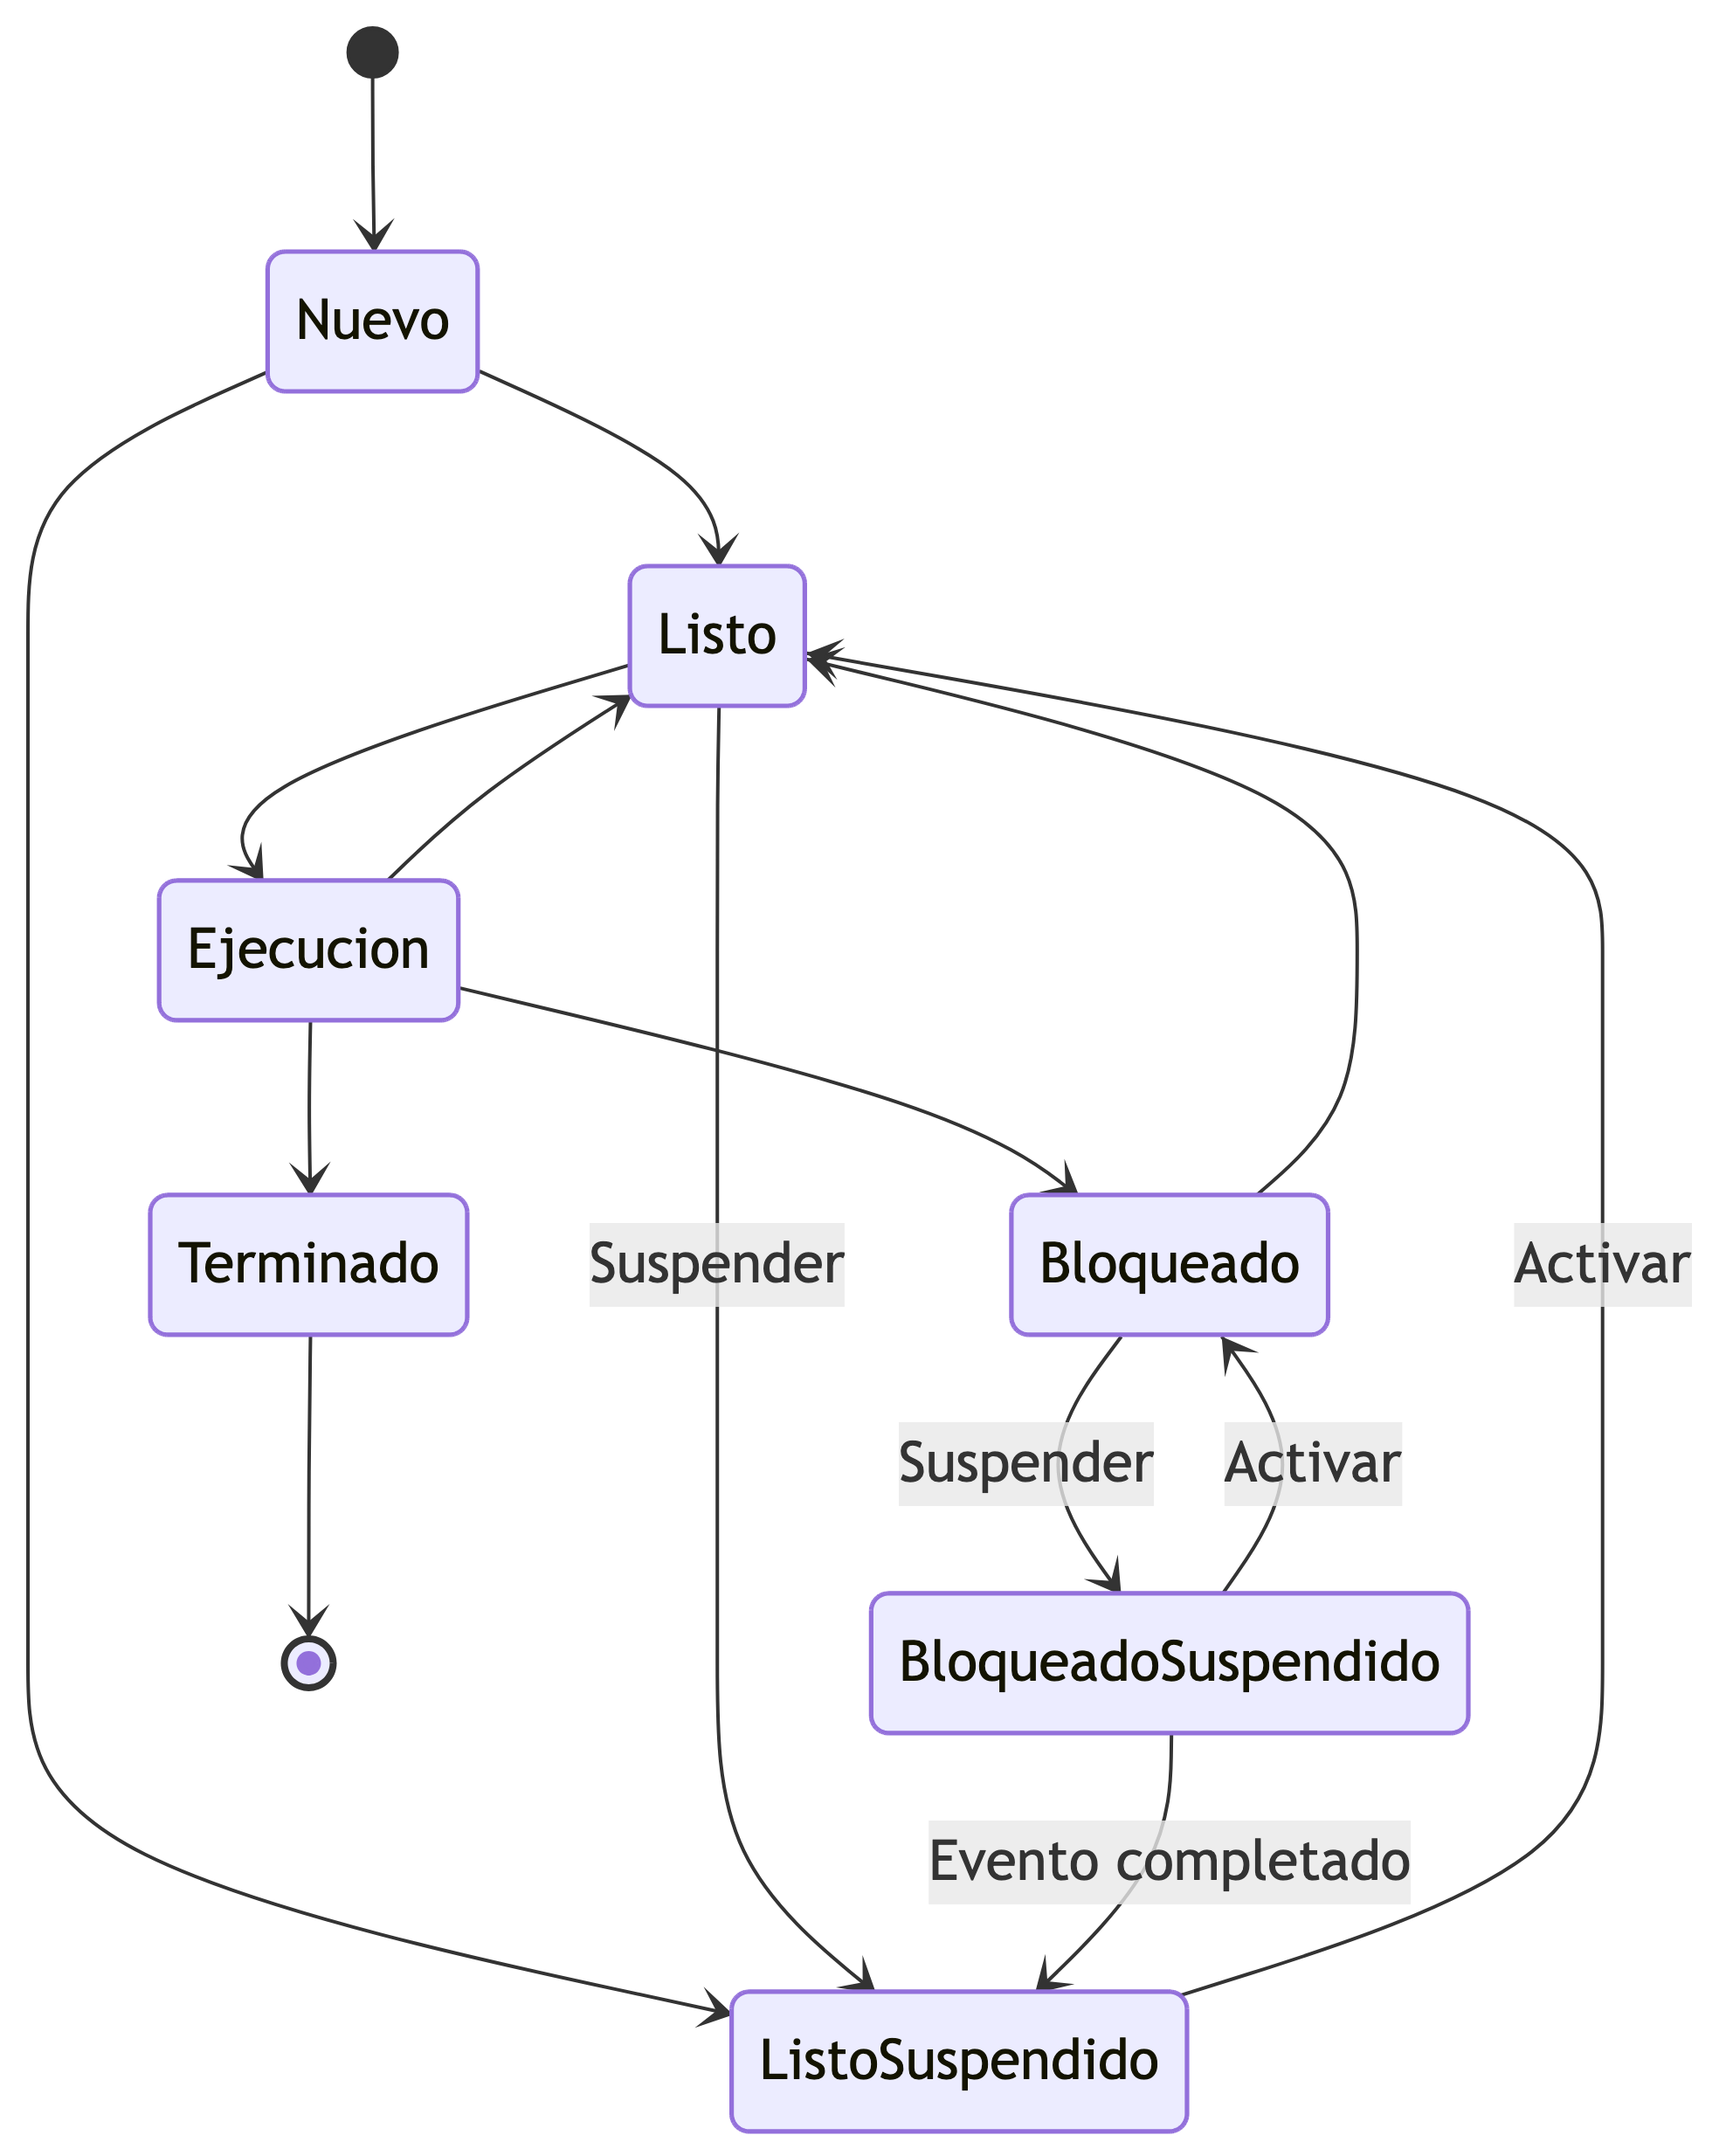
\includegraphics[width=5.13in,height=6.44in]{capitulos/04_administracion_procesos_files/figure-latex/mermaid-figure-5.png}

\subsection{Nuevos estados}\label{nuevos-estados}

{\def\LTcaptype{none} % do not increment counter
\begin{longtable}[]{@{}
  >{\raggedright\arraybackslash}p{(\linewidth - 2\tabcolsep) * \real{0.4091}}
  >{\raggedright\arraybackslash}p{(\linewidth - 2\tabcolsep) * \real{0.5909}}@{}}
\toprule\noalign{}
\begin{minipage}[b]{\linewidth}\raggedright
Estado
\end{minipage} & \begin{minipage}[b]{\linewidth}\raggedright
Descripción
\end{minipage} \\
\midrule\noalign{}
\endhead
\bottomrule\noalign{}
\endlastfoot
\textbf{Listo y Suspendido} & El proceso está preparado para ejecutarse,
pero fue trasladado al disco porque no existe memoria RAM suficiente. \\
\textbf{Bloqueado y Suspendido} & El proceso permanece esperando un
evento y, además, fue movido temporalmente al almacenamiento
secundario. \\
\end{longtable}
}

\begin{tcolorbox}[enhanced jigsaw, arc=.35mm, bottomrule=.15mm, bottomtitle=1mm, breakable, colback=white, colbacktitle=quarto-callout-note-color!10!white, colframe=quarto-callout-note-color-frame, coltitle=black, left=2mm, leftrule=.75mm, opacityback=0, opacitybacktitle=0.6, rightrule=.15mm, title=\textcolor{quarto-callout-note-color}{\faInfo}\hspace{0.5em}{¿Qué es el Swap?}, titlerule=0mm, toprule=.15mm, toptitle=1mm]

El \textbf{Swap} consiste en mover procesos completos o parte de su
memoria desde la RAM hacia un área especial del disco duro o del SSD
para liberar memoria física y permitir que otros procesos continúen
ejecutándose.

Aunque esta técnica incrementa la capacidad de ejecución del sistema,
también reduce el rendimiento, ya que acceder al disco es mucho más
lento que acceder a la memoria RAM.

\end{tcolorbox}

\bookmarksetup{startatroot}

\chapter{Resumen}\label{resumen}

\begin{itemize}
\tightlist
\item
  Un programa se convierte en proceso al ejecutarse.
\item
  Cada proceso posee memoria y recursos propios.
\item
  El PCB almacena toda la información necesaria para administrarlo.
\item
  El Scheduler comparte el procesador entre todos los procesos.
\item
  En la siguiente sección estudiaremos el ciclo de vida y los estados de
  un proceso.
\end{itemize}

\bookmarksetup{startatroot}

\chapter{Scheduler y Dispatcher}\label{scheduler-y-dispatcher}

El \textbf{Scheduler} decide qué proceso obtendrá el procesador cuando
existen varios procesos listos para ejecutarse. Para tomar esta decisión
puede considerar la prioridad, el tiempo de espera o el algoritmo de
planificación configurado por el sistema operativo.

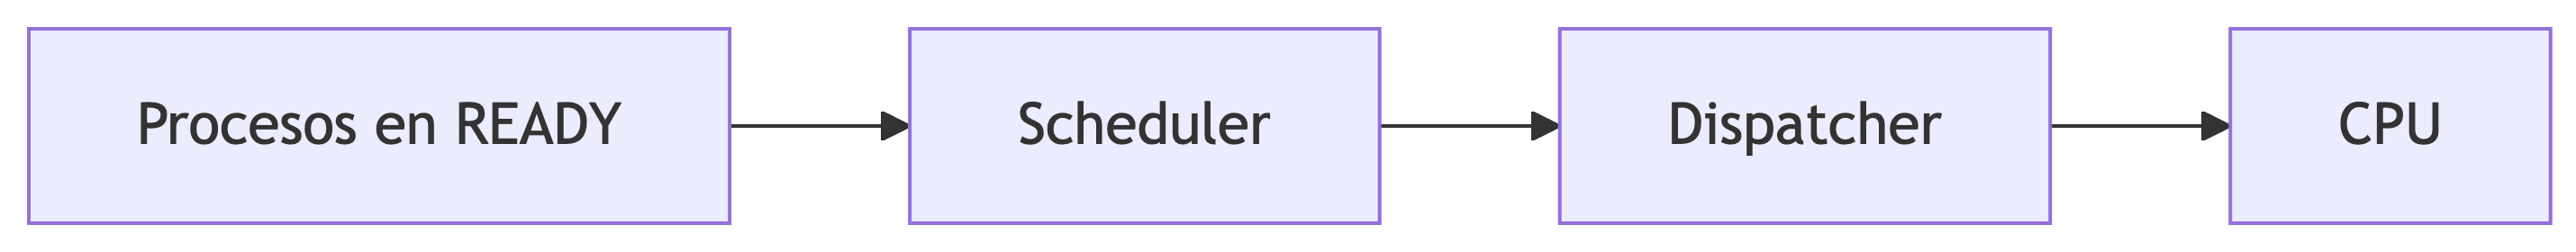
\includegraphics[width=7.46in,height=0.73in]{capitulos/04_administracion_procesos_files/figure-latex/mermaid-figure-4.png}

El \textbf{Dispatcher} es el componente encargado de entregar realmente
la CPU al proceso seleccionado y realizar el cambio de contexto.

\bookmarksetup{startatroot}

\chapter{Cambio de contexto (Context
Switch)}\label{cambio-de-contexto-context-switch}

Un cambio de contexto ocurre cuando el sistema operativo detiene
temporalmente un proceso, guarda su estado en el PCB y restaura el
estado de otro proceso.

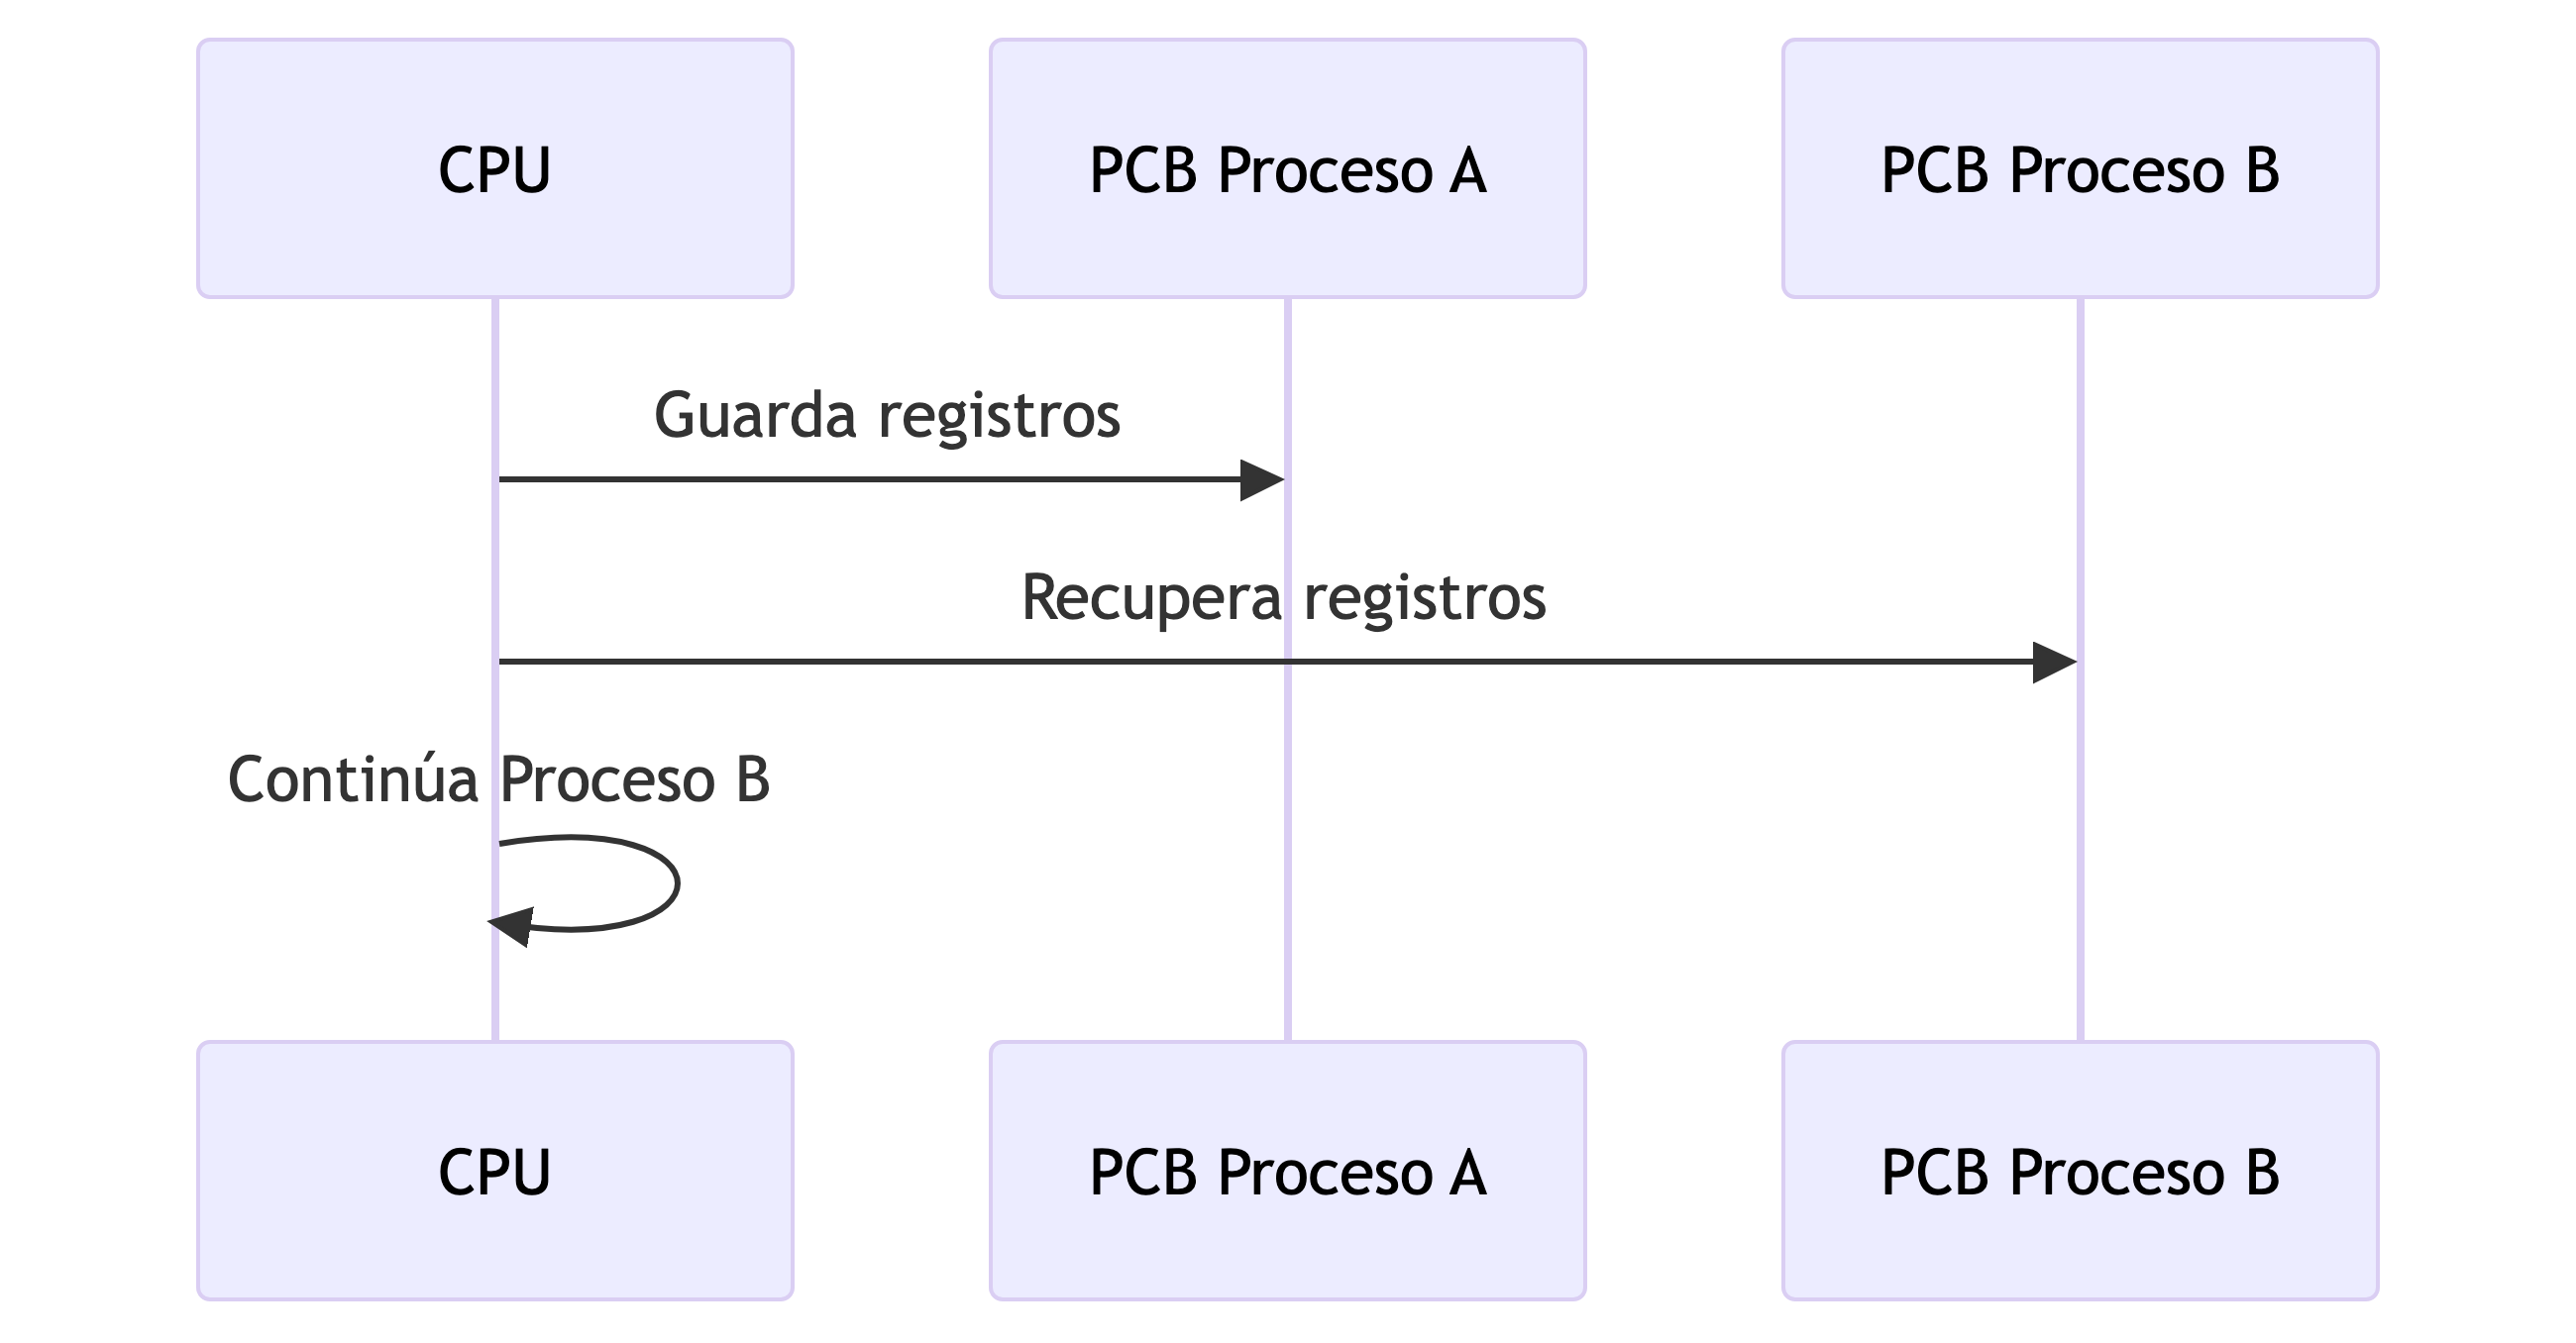
\includegraphics[width=6.77in,height=3.53in]{capitulos/04_administracion_procesos_files/figure-latex/mermaid-figure-3.png}

\bookmarksetup{startatroot}

\chapter{Ejemplo completo: Microsoft
Word}\label{ejemplo-completo-microsoft-word}

\begin{enumerate}
\def\labelenumi{\arabic{enumi}.}
\tightlist
\item
  El usuario hace doble clic sobre \textbf{Word.exe}.
\item
  El Kernel crea el proceso y asigna un PID.
\item
  El proceso entra al estado \textbf{NEW}.
\item
  Se reserva memoria y se crea el PCB.
\item
  El proceso pasa a \textbf{READY}.
\item
  El Scheduler selecciona el proceso.
\item
  El Dispatcher entrega la CPU.
\item
  El proceso entra en \textbf{RUNNING}.
\item
  Al guardar un archivo, espera la respuesta del disco
  (\textbf{WAITING}).
\item
  Finalizada la operación de E/S vuelve a \textbf{READY}.
\item
  El Scheduler le asigna nuevamente la CPU.
\item
  Al cerrar Word, el proceso entra en \textbf{EXIT} y el sistema libera
  memoria, archivos y demás recursos.
\end{enumerate}

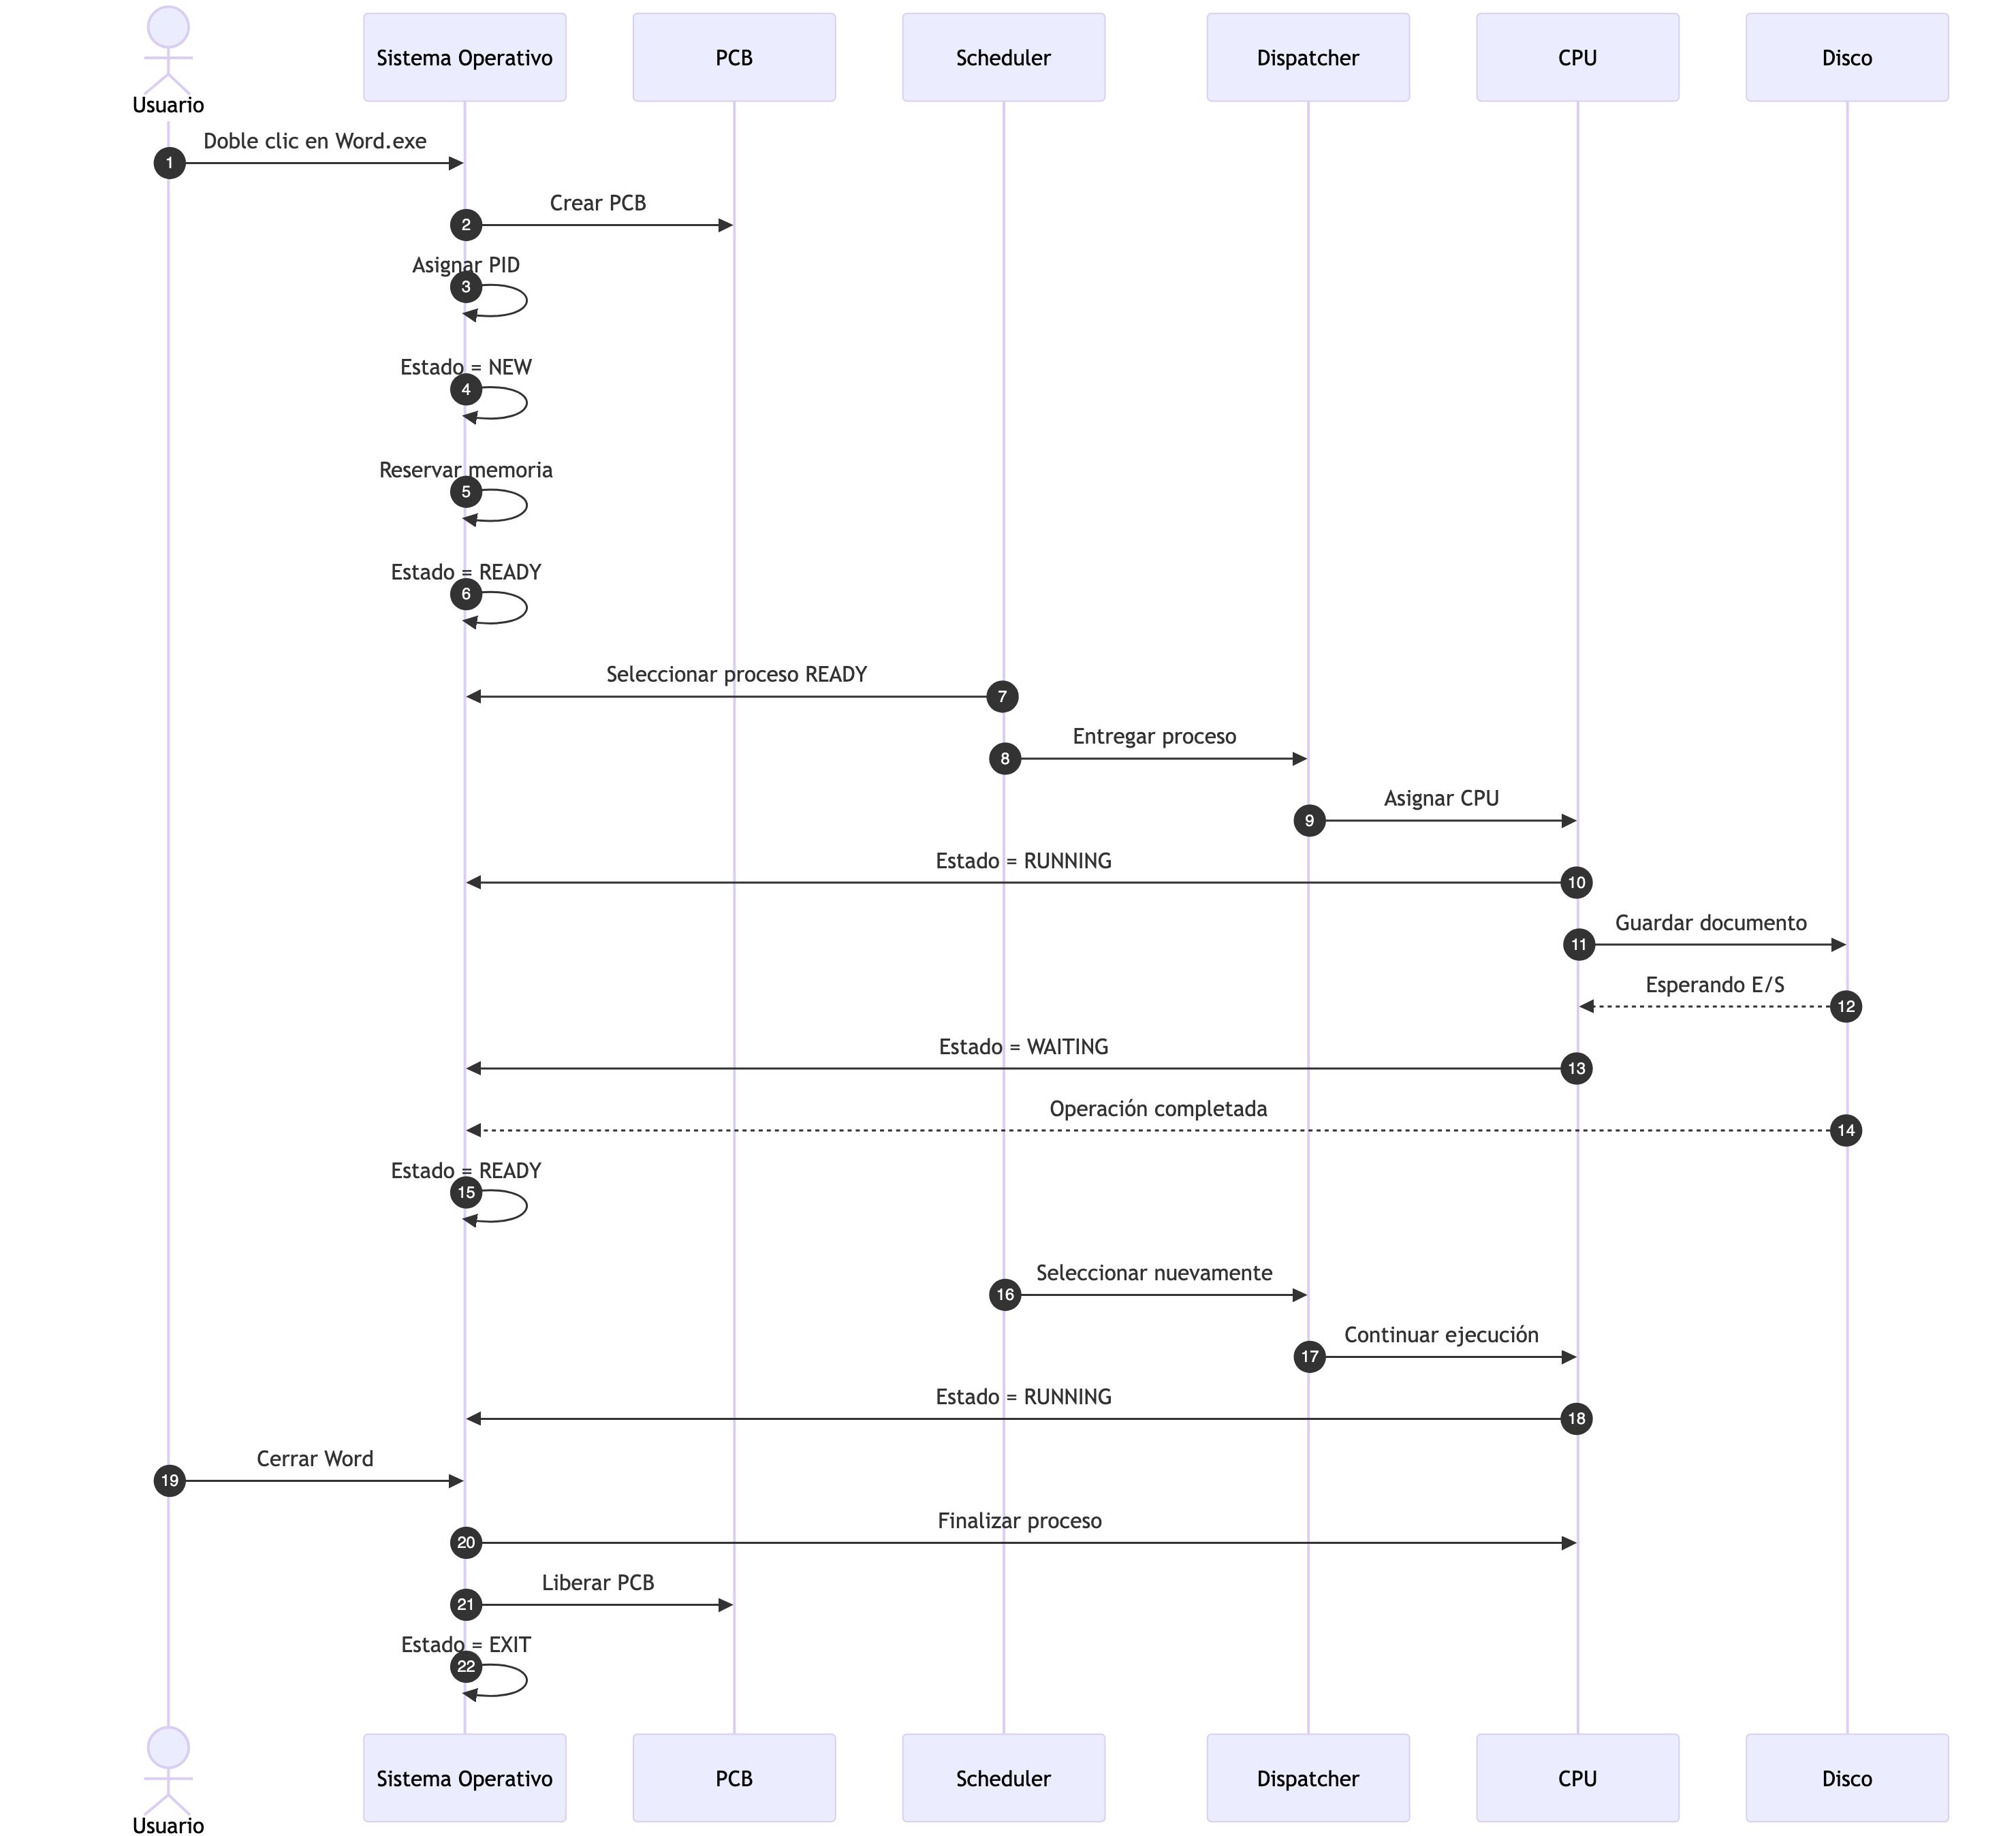
\includegraphics[width=6.2in,height=8.4in]{capitulos/04_administracion_procesos_files/figure-latex/mermaid-figure-2.png}

\section{Autoevaluación}\label{autoevaluaciuxf3n-1}

\begin{enumerate}
\def\labelenumi{\arabic{enumi}.}
\tightlist
\item
  ¿Cuál es la diferencia entre un programa y un proceso?
\item
  ¿Qué información almacena el PCB?
\item
  ¿Qué función cumple el Scheduler?
\item
  ¿Cuándo ocurre un cambio de contexto?
\item
  Explique el recorrido NEW → READY → RUNNING → WAITING → READY → EXIT
  con sus propias palabras.
\end{enumerate}

\bookmarksetup{startatroot}

\chapter{Clase 5. Control de Procesos y
Concurrencia}\label{clase-5.-control-de-procesos-y-concurrencia}

\bookmarksetup{startatroot}

\chapter{Clase 5. Control de Procesos y
Concurrencia}\label{clase-5.-control-de-procesos-y-concurrencia-1}

\section{Presentación de la clase}\label{presentaciuxf3n-de-la-clase-3}

En la clase anterior estudiamos cómo el sistema operativo crea, registra
y administra los procesos mediante estructuras como el \textbf{PCB}, la
tabla de procesos, el \textbf{Scheduler}, el \textbf{Dispatcher} y los
cambios de contexto.

En esta clase ampliaremos esa base para comprender cómo el sistema
operativo controla varios procesos e hilos que avanzan de forma
concurrente, cómo distribuye el tiempo del procesador y qué problemas
aparecen cuando varias unidades de ejecución comparten datos o recursos.

También analizaremos el papel real que puede desempeñar la inteligencia
artificial en la administración de recursos. La IA no sustituye al
kernel ni modifica por sí misma el PCB; puede emplearse como apoyo para
construir políticas de planificación, predicción y detección de
anomalías.

\begin{tcolorbox}[enhanced jigsaw, arc=.35mm, bottomrule=.15mm, bottomtitle=1mm, breakable, colback=white, colbacktitle=quarto-callout-note-color!10!white, colframe=quarto-callout-note-color-frame, coltitle=black, left=2mm, leftrule=.75mm, opacityback=0, opacitybacktitle=0.6, rightrule=.15mm, title=\textcolor{quarto-callout-note-color}{\faInfo}\hspace{0.5em}{Pregunta detonadora}, titlerule=0mm, toprule=.15mm, toptitle=1mm]

Cuando un navegador reproduce música, descarga un archivo, muestra
varias pestañas y responde al teclado casi al mismo tiempo, ¿cómo evita
el sistema operativo que todas esas actividades interfieran entre sí?

\end{tcolorbox}

\section{Objetivos de aprendizaje}\label{objetivos-de-aprendizaje-3}

Al finalizar la clase, el estudiante será capaz de:

\begin{enumerate}
\def\labelenumi{\arabic{enumi}.}
\tightlist
\item
  Explicar qué significa controlar un proceso.
\item
  Diferenciar procesos e hilos.
\item
  Comprender la relación entre concurrencia y paralelismo.
\item
  Explicar el propósito del quantum de tiempo.
\item
  Relacionar el quantum con la planificación Round Robin.
\item
  Identificar los componentes principales del PCB.
\item
  Reconocer una sección crítica y una condición de carrera.
\item
  Explicar la finalidad de la exclusión mutua.
\item
  Interpretar el algoritmo de Dekker como una solución histórica para
  dos procesos.
\item
  Analizar, con criterio técnico, posibles aplicaciones de inteligencia
  artificial en la administración de recursos.
\end{enumerate}

\section{Ruta de aprendizaje}\label{ruta-de-aprendizaje-1}

La clase seguirá esta secuencia:

\begin{enumerate}
\def\labelenumi{\arabic{enumi}.}
\tightlist
\item
  Control del ciclo de vida de los procesos.
\item
  Diferencia entre proceso e hilo.
\item
  Concurrencia y paralelismo.
\item
  Quantum y planificación Round Robin.
\item
  PCB y cambio de contexto.
\item
  Recursos compartidos y condiciones de carrera.
\item
  Sección crítica y exclusión mutua.
\item
  Algoritmo de Dekker.
\item
  IA aplicada a planificación y observabilidad.
\item
  Caso integrador, laboratorio y autoevaluación.
\end{enumerate}

\bookmarksetup{startatroot}

\chapter{¿Qué es el control de
procesos?}\label{quuxe9-es-el-control-de-procesos}

El \textbf{control de procesos} es el conjunto de mecanismos utilizados
por el sistema operativo para crear, registrar, planificar, pausar,
reanudar, sincronizar y finalizar procesos.

El sistema operativo no se limita a ``abrir programas''. Debe mantener
una visión organizada de todo lo que se encuentra en ejecución.

Entre sus responsabilidades están:

\begin{itemize}
\tightlist
\item
  crear el proceso;
\item
  asignarle un identificador;
\item
  reservar memoria;
\item
  crear y actualizar su PCB;
\item
  ubicarlo en una cola de planificación;
\item
  asignarle tiempo de CPU;
\item
  atender solicitudes de entrada y salida;
\item
  proteger sus recursos;
\item
  coordinar su comunicación con otros procesos;
\item
  finalizarlo y liberar los recursos utilizados.
\end{itemize}

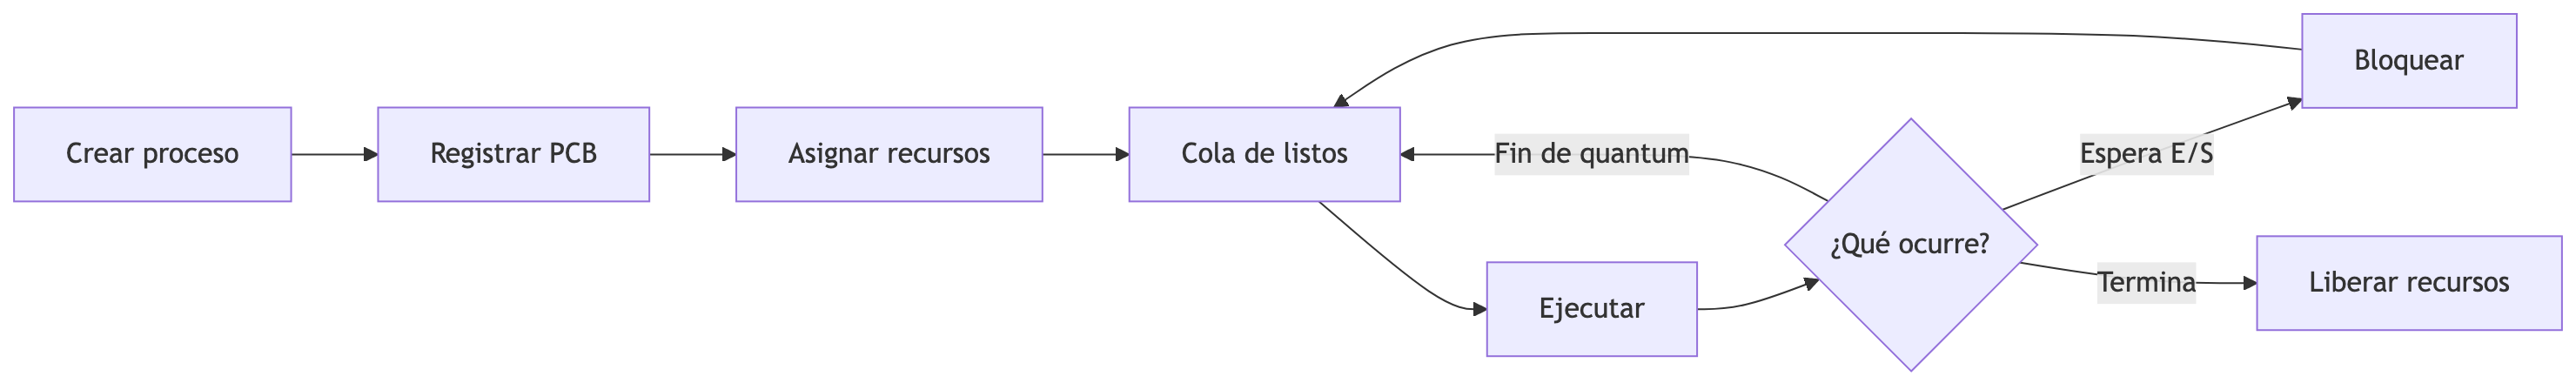
\includegraphics[width=6.2in,height=4.2in]{capitulos/05_control_procesos_concurrencia_files/figure-latex/mermaid-figure-1.png}

\begin{tcolorbox}[enhanced jigsaw, arc=.35mm, bottomrule=.15mm, bottomtitle=1mm, breakable, colback=white, colbacktitle=quarto-callout-tip-color!10!white, colframe=quarto-callout-tip-color-frame, coltitle=black, left=2mm, leftrule=.75mm, opacityback=0, opacitybacktitle=0.6, rightrule=.15mm, title=\textcolor{quarto-callout-tip-color}{\faLightbulb}\hspace{0.5em}{Idea central}, titlerule=0mm, toprule=.15mm, toptitle=1mm]

Controlar un proceso significa conservar suficiente información para
detenerlo, reanudarlo y finalizarlo sin perder la coherencia de su
ejecución.

\end{tcolorbox}

\bookmarksetup{startatroot}

\chapter{Proceso e hilo}\label{proceso-e-hilo}

\section{Proceso}\label{proceso}

Un \textbf{proceso} es una instancia de un programa en ejecución. Posee
su propio espacio de direcciones y los recursos que el sistema operativo
le ha asignado.

Un proceso normalmente incluye:

\begin{itemize}
\tightlist
\item
  código;
\item
  datos;
\item
  heap;
\item
  stack;
\item
  archivos abiertos;
\item
  credenciales y permisos;
\item
  uno o más hilos;
\item
  un PCB o estructura equivalente mantenida por el kernel.
\end{itemize}

\section{Hilo}\label{hilo}

Un \textbf{hilo} o \textbf{thread} es una unidad de ejecución dentro de
un proceso.

Los hilos de un mismo proceso suelen compartir:

\begin{itemize}
\tightlist
\item
  código;
\item
  datos globales;
\item
  heap;
\item
  archivos abiertos;
\item
  espacio de direcciones.
\end{itemize}

Cada hilo conserva elementos propios, como:

\begin{itemize}
\tightlist
\item
  contador de programa;
\item
  registros;
\item
  stack;
\item
  estado de ejecución;
\item
  identificador del hilo.
\end{itemize}

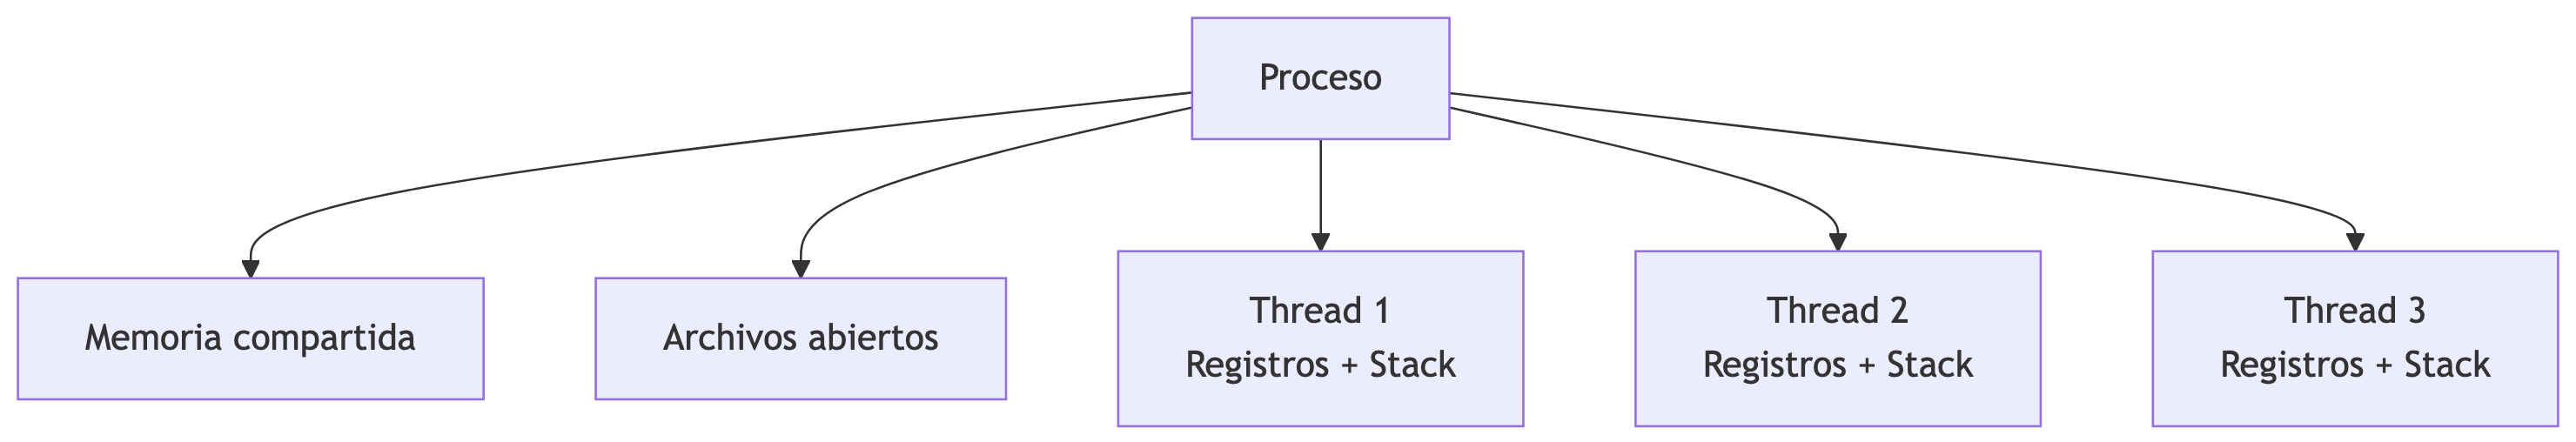
\includegraphics[width=6.2in,height=4.5in]{capitulos/05_control_procesos_concurrencia_files/figure-latex/mermaid-figure-11.png}

\section{Comparación}\label{comparaciuxf3n}

{\def\LTcaptype{none} % do not increment counter
\begin{longtable}[]{@{}
  >{\raggedright\arraybackslash}p{(\linewidth - 4\tabcolsep) * \real{0.3333}}
  >{\raggedright\arraybackslash}p{(\linewidth - 4\tabcolsep) * \real{0.3333}}
  >{\raggedright\arraybackslash}p{(\linewidth - 4\tabcolsep) * \real{0.3333}}@{}}
\toprule\noalign{}
\begin{minipage}[b]{\linewidth}\raggedright
Característica
\end{minipage} & \begin{minipage}[b]{\linewidth}\raggedright
Proceso
\end{minipage} & \begin{minipage}[b]{\linewidth}\raggedright
Hilo
\end{minipage} \\
\midrule\noalign{}
\endhead
\bottomrule\noalign{}
\endlastfoot
Espacio de memoria & Generalmente independiente & Comparte el espacio
del proceso \\
Costo de creación & Mayor & Menor \\
Comunicación & Requiere mecanismos de IPC & Puede compartir variables y
estructuras \\
Aislamiento & Mayor & Menor \\
Fallo & Puede quedar aislado & Puede afectar al proceso completo \\
Uso típico & Aplicaciones o servicios separados & Tareas relacionadas
dentro de una aplicación \\
\end{longtable}
}

\begin{tcolorbox}[enhanced jigsaw, arc=.35mm, bottomrule=.15mm, bottomtitle=1mm, breakable, colback=white, colbacktitle=quarto-callout-warning-color!10!white, colframe=quarto-callout-warning-color-frame, coltitle=black, left=2mm, leftrule=.75mm, opacityback=0, opacitybacktitle=0.6, rightrule=.15mm, title=\textcolor{quarto-callout-warning-color}{\faExclamationTriangle}\hspace{0.5em}{Precisión importante}, titlerule=0mm, toprule=.15mm, toptitle=1mm]

No debe afirmarse que cada pestaña de un navegador siempre corresponde a
un hilo. Los navegadores modernos pueden utilizar una arquitectura
multiproceso y, dentro de cada proceso, varios hilos. La implementación
exacta depende del navegador y de su modelo de aislamiento.

\end{tcolorbox}

\bookmarksetup{startatroot}

\chapter{Concurrencia y paralelismo}\label{concurrencia-y-paralelismo}

Estos conceptos están relacionados, pero no significan lo mismo.

\section{Concurrencia}\label{concurrencia}

Existe \textbf{concurrencia} cuando varias tareas progresan durante un
mismo período, aunque no necesariamente se ejecuten exactamente al mismo
tiempo.

En una CPU de un solo núcleo, el sistema puede intercalar rápidamente la
ejecución:

\begin{Shaded}
\begin{Highlighting}[]
\NormalTok{Proceso A → Proceso B → Proceso C → Proceso A → ...}
\end{Highlighting}
\end{Shaded}

\section{Paralelismo}\label{paralelismo}

Existe \textbf{paralelismo} cuando dos o más tareas se ejecutan
físicamente al mismo tiempo, por ejemplo, en núcleos diferentes.

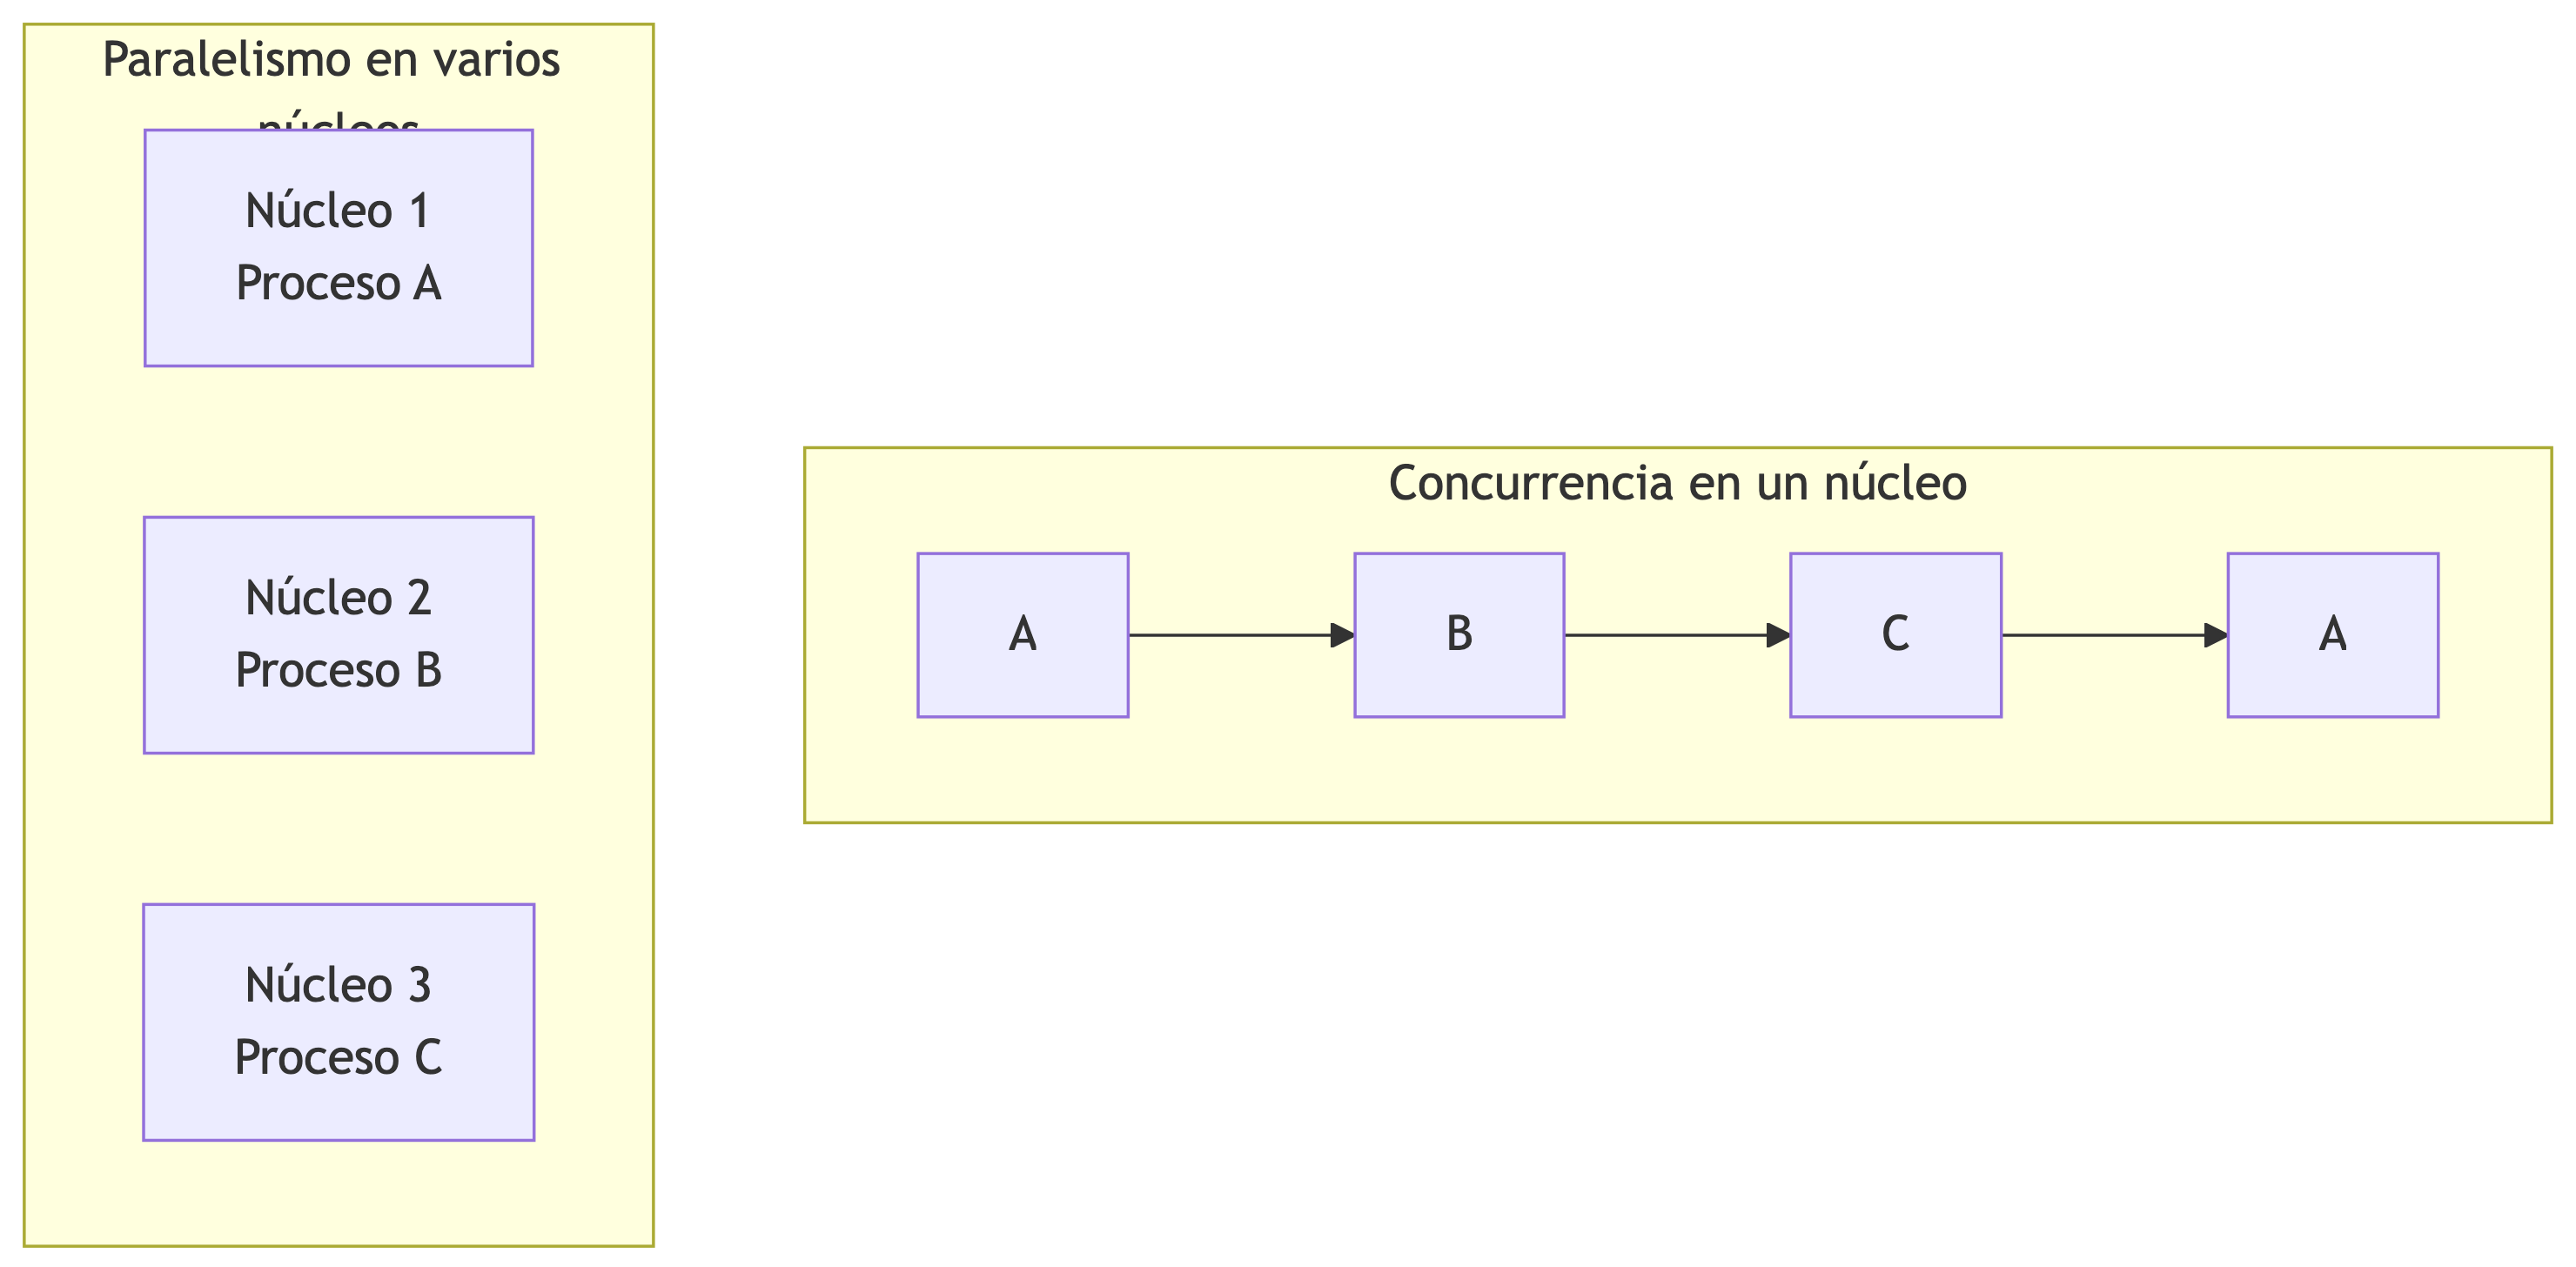
\includegraphics[width=6.2in,height=4.5in]{capitulos/05_control_procesos_concurrencia_files/figure-latex/mermaid-figure-10.png}

{\def\LTcaptype{none} % do not increment counter
\begin{longtable}[]{@{}
  >{\raggedright\arraybackslash}p{(\linewidth - 2\tabcolsep) * \real{0.5000}}
  >{\raggedright\arraybackslash}p{(\linewidth - 2\tabcolsep) * \real{0.5000}}@{}}
\toprule\noalign{}
\begin{minipage}[b]{\linewidth}\raggedright
Concepto
\end{minipage} & \begin{minipage}[b]{\linewidth}\raggedright
Pregunta clave
\end{minipage} \\
\midrule\noalign{}
\endhead
\bottomrule\noalign{}
\endlastfoot
Concurrencia & ¿Varias tareas avanzan durante el mismo período? \\
Paralelismo & ¿Varias tareas se ejecutan simultáneamente en hardware
distinto? \\
\end{longtable}
}

\begin{tcolorbox}[enhanced jigsaw, arc=.35mm, bottomrule=.15mm, bottomtitle=1mm, breakable, colback=white, colbacktitle=quarto-callout-note-color!10!white, colframe=quarto-callout-note-color-frame, coltitle=black, left=2mm, leftrule=.75mm, opacityback=0, opacitybacktitle=0.6, rightrule=.15mm, title=\textcolor{quarto-callout-note-color}{\faInfo}\hspace{0.5em}{Ejemplo}, titlerule=0mm, toprule=.15mm, toptitle=1mm]

Una persona puede atender concurrentemente varias conversaciones
alternando entre ellas. Dos personas pueden atender conversaciones en
paralelo.

\end{tcolorbox}

\bookmarksetup{startatroot}

\chapter{Quantum de tiempo}\label{quantum-de-tiempo}

El \textbf{quantum}, también llamado \textbf{time slice}, es el
intervalo máximo durante el cual un proceso puede conservar la CPU antes
de ser interrumpido por el planificador, siempre que no se bloquee o
termine antes.

El quantum es especialmente importante en algoritmos de planificación
apropiativos como \textbf{Round Robin}.

\section{¿Qué ocurre cuando termina el
quantum?}\label{quuxe9-ocurre-cuando-termina-el-quantum}

\begin{enumerate}
\def\labelenumi{\arabic{enumi}.}
\tightlist
\item
  El reloj genera una interrupción.
\item
  El kernel recupera el control.
\item
  Se guarda el contexto del proceso.
\item
  El proceso pasa de Ejecución a Listo.
\item
  El Scheduler selecciona otro proceso.
\item
  El Dispatcher restaura su contexto.
\item
  El nuevo proceso continúa ejecutándose.
\end{enumerate}

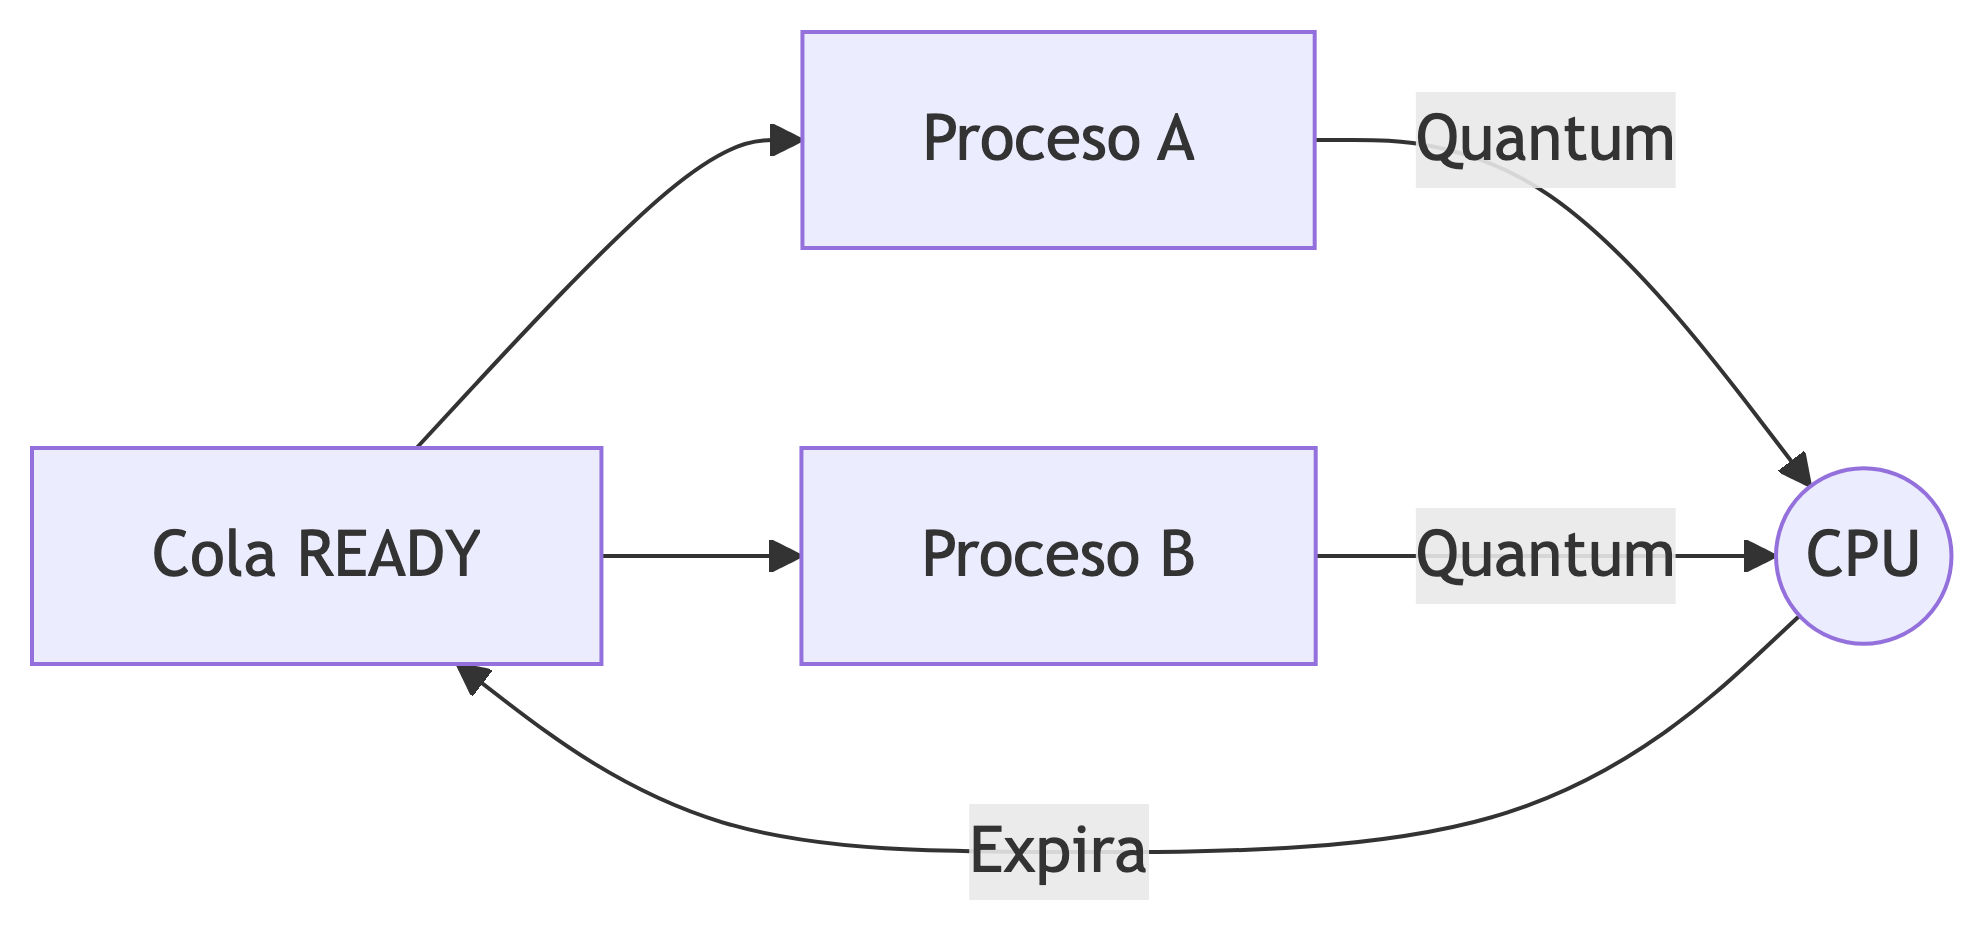
\includegraphics[width=6.2in,height=4.1in]{capitulos/05_control_procesos_concurrencia_files/figure-latex/mermaid-figure-9.png}

\section{Efecto del tamaño del
quantum}\label{efecto-del-tamauxf1o-del-quantum}

{\def\LTcaptype{none} % do not increment counter
\begin{longtable}[]{@{}
  >{\raggedright\arraybackslash}p{(\linewidth - 4\tabcolsep) * \real{0.3333}}
  >{\raggedright\arraybackslash}p{(\linewidth - 4\tabcolsep) * \real{0.3333}}
  >{\raggedright\arraybackslash}p{(\linewidth - 4\tabcolsep) * \real{0.3333}}@{}}
\toprule\noalign{}
\begin{minipage}[b]{\linewidth}\raggedright
Quantum
\end{minipage} & \begin{minipage}[b]{\linewidth}\raggedright
Ventaja
\end{minipage} & \begin{minipage}[b]{\linewidth}\raggedright
Riesgo
\end{minipage} \\
\midrule\noalign{}
\endhead
\bottomrule\noalign{}
\endlastfoot
Muy pequeño & Mayor sensación de respuesta & Más cambios de contexto \\
Moderado & Equilibrio entre respuesta y costo & Debe adaptarse al
sistema \\
Muy grande & Menos cambios de contexto & Se aproxima a FCFS y reduce
interactividad \\
\end{longtable}
}

\begin{tcolorbox}[enhanced jigsaw, arc=.35mm, bottomrule=.15mm, bottomtitle=1mm, breakable, colback=white, colbacktitle=quarto-callout-important-color!10!white, colframe=quarto-callout-important-color-frame, coltitle=black, left=2mm, leftrule=.75mm, opacityback=0, opacitybacktitle=0.6, rightrule=.15mm, title=\textcolor{quarto-callout-important-color}{\faExclamation}\hspace{0.5em}{No existe un quantum universal}, titlerule=0mm, toprule=.15mm, toptitle=1mm]

El valor apropiado depende de la carga, el hardware, los objetivos de
respuesta y la política del sistema operativo.

\end{tcolorbox}

\bookmarksetup{startatroot}

\chapter{Planificación Round Robin}\label{planificaciuxf3n-round-robin}

\textbf{Round Robin} organiza los procesos listos en una cola y asigna a
cada uno un quantum de CPU.

Supongamos:

\begin{Shaded}
\begin{Highlighting}[]
\NormalTok{Quantum = 4 unidades}
\end{Highlighting}
\end{Shaded}

y tres procesos:

{\def\LTcaptype{none} % do not increment counter
\begin{longtable}[]{@{}lr@{}}
\toprule\noalign{}
Proceso & Ráfaga de CPU \\
\midrule\noalign{}
\endhead
\bottomrule\noalign{}
\endlastfoot
P1 & 9 \\
P2 & 5 \\
P3 & 3 \\
\end{longtable}
}

La ejecución inicial sería:

\begin{Shaded}
\begin{Highlighting}[]
\NormalTok{0       4       8      11      15      16      17}
\NormalTok{|  P1   |  P2   | P3  |  P1   |  P2  | P1 |}
\end{Highlighting}
\end{Shaded}

\subsection{Interpretación}\label{interpretaciuxf3n}

\begin{itemize}
\tightlist
\item
  P1 utiliza 4 unidades y necesita 5 más.
\item
  P2 utiliza 4 unidades y necesita 1 más.
\item
  P3 necesita solo 3 y termina en su primer turno.
\item
  P1 utiliza otras 4 y necesita 1.
\item
  P2 termina.
\item
  P1 termina.
\end{itemize}

\begin{tcolorbox}[enhanced jigsaw, arc=.35mm, bottomrule=.15mm, bottomtitle=1mm, breakable, colback=white, colbacktitle=quarto-callout-tip-color!10!white, colframe=quarto-callout-tip-color-frame, coltitle=black, left=2mm, leftrule=.75mm, opacityback=0, opacitybacktitle=0.6, rightrule=.15mm, title=\textcolor{quarto-callout-tip-color}{\faLightbulb}\hspace{0.5em}{Ventaja de Round Robin}, titlerule=0mm, toprule=.15mm, toptitle=1mm]

Todos los procesos listos reciben oportunidades periódicas de ejecución,
lo que favorece la interactividad y evita que uno monopolice
indefinidamente la CPU.

\end{tcolorbox}

\bookmarksetup{startatroot}

\chapter{PCB y control del proceso}\label{pcb-y-control-del-proceso}

El \textbf{Process Control Block} es la estructura mediante la cual el
sistema operativo conserva la información necesaria para administrar un
proceso.

\section{Componentes principales}\label{componentes-principales}

{\def\LTcaptype{none} % do not increment counter
\begin{longtable}[]{@{}
  >{\raggedright\arraybackslash}p{(\linewidth - 2\tabcolsep) * \real{0.5000}}
  >{\raggedright\arraybackslash}p{(\linewidth - 2\tabcolsep) * \real{0.5000}}@{}}
\toprule\noalign{}
\begin{minipage}[b]{\linewidth}\raggedright
Categoría
\end{minipage} & \begin{minipage}[b]{\linewidth}\raggedright
Información
\end{minipage} \\
\midrule\noalign{}
\endhead
\bottomrule\noalign{}
\endlastfoot
Identificación & PID, PPID, usuario y grupo \\
Estado & Nuevo, listo, ejecución, bloqueado o terminado \\
Contexto de CPU & Registros, contador de programa y puntero de pila \\
Planificación & Prioridad, política, tiempo utilizado y afinidad \\
Memoria & Espacio de direcciones y estructuras de administración \\
Entrada/salida & Dispositivos, operaciones pendientes y archivos
abiertos \\
Seguridad & Credenciales, privilegios y permisos \\
Contabilidad & Tiempo de CPU, fecha de creación y estadísticas \\
\end{longtable}
}

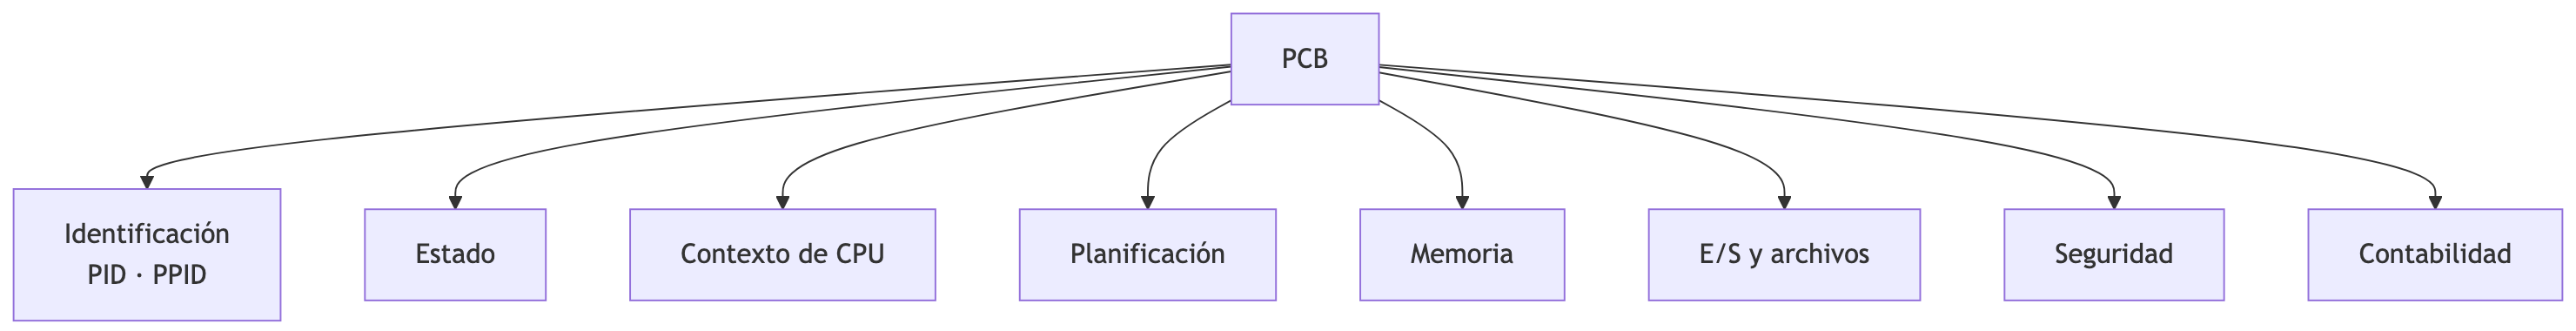
\includegraphics[width=6.2in,height=5.2in]{capitulos/05_control_procesos_concurrencia_files/figure-latex/mermaid-figure-8.png}

\begin{tcolorbox}[enhanced jigsaw, arc=.35mm, bottomrule=.15mm, bottomtitle=1mm, breakable, colback=white, colbacktitle=quarto-callout-warning-color!10!white, colframe=quarto-callout-warning-color-frame, coltitle=black, left=2mm, leftrule=.75mm, opacityback=0, opacitybacktitle=0.6, rightrule=.15mm, title=\textcolor{quarto-callout-warning-color}{\faExclamationTriangle}\hspace{0.5em}{Modelo conceptual}, titlerule=0mm, toprule=.15mm, toptitle=1mm]

Los nombres y campos exactos varían entre sistemas operativos. ``PCB''
es una forma didáctica de agrupar la información; un kernel real puede
distribuirla entre varias estructuras internas.

\end{tcolorbox}

\bookmarksetup{startatroot}

\chapter{Cambio de contexto}\label{cambio-de-contexto}

Un \textbf{cambio de contexto} ocurre cuando la CPU deja de ejecutar una
unidad de trabajo y comienza otra.

\section{Del mundo real al Sistema
Operativo}\label{del-mundo-real-al-sistema-operativo}

\begin{tcolorbox}[enhanced jigsaw, arc=.35mm, bottomrule=.15mm, breakable, colback=white, colframe=quarto-callout-tip-color-frame, left=2mm, leftrule=.75mm, opacityback=0, rightrule=.15mm, toprule=.15mm]

\vspace{-3mm}\textbf{🍽️ Analogía: El mesero del restaurante}\vspace{3mm}

Imagina un restaurante donde \textbf{solo hay un mesero} atendiendo
varias mesas.

En la \textbf{Mesa A} una familia está haciendo su pedido, pero mientras
el mesero la atiende, llega una nueva familia a la \textbf{Mesa B}.

El administrador le pide que primero reciba a los nuevos clientes.

Antes de irse, el mesero \textbf{anota exactamente en qué punto quedó
atendiendo la Mesa A} para no olvidar ningún detalle.

Después atiende la Mesa B y, cuando termina, regresa a la Mesa A.
Gracias a las anotaciones de su libreta puede continuar exactamente
donde había quedado.

La CPU realiza un proceso muy similar cuando cambia de un proceso a
otro.

\end{tcolorbox}

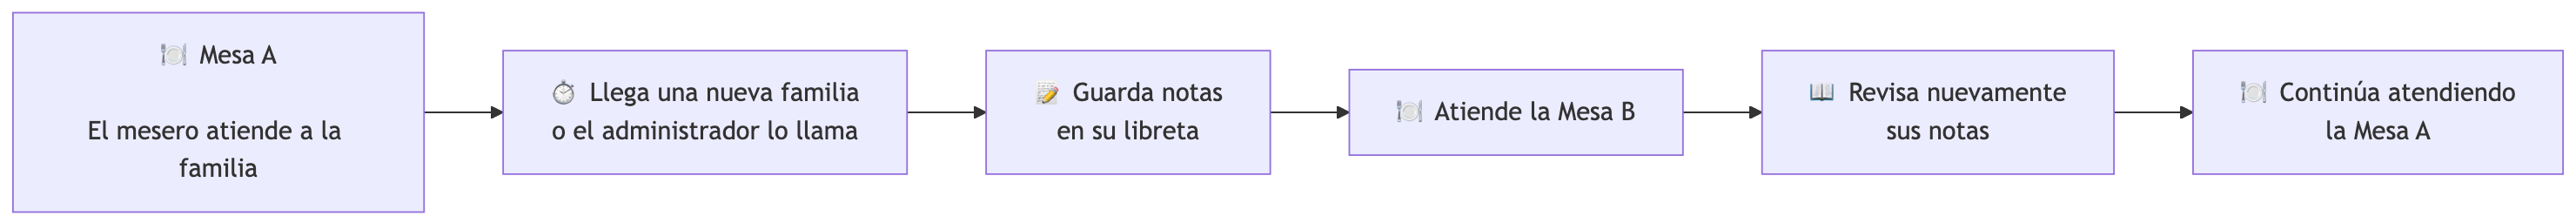
\includegraphics[width=16.97in,height=1.48in]{capitulos/05_control_procesos_concurrencia_files/figure-latex/mermaid-figure-7.png}

\emph{Flujo}

\begin{verbatim}
1. El mesero atiende a la **Mesa A**.
2. Ocurre una **interrupción**.
3. Guarda notas en su libreta.
4. Atiende la **Mesa B**.
5. Recupera sus notas.
6. Continúa atendiendo la **Mesa A**.
\end{verbatim}

\subsection{Relación entre el restaurante y el Sistema
Operativo}\label{relaciuxf3n-entre-el-restaurante-y-el-sistema-operativo}

{\def\LTcaptype{none} % do not increment counter
\begin{longtable}[]{@{}ll@{}}
\toprule\noalign{}
En el restaurante & En el Sistema Operativo \\
\midrule\noalign{}
\endhead
\bottomrule\noalign{}
\endlastfoot
Mesero & CPU \\
Mesa A & Proceso A \\
Mesa B & Proceso B \\
Libreta del mesero & PCB (Process Control Block) \\
Administrador & Kernel \\
Cambiar de una mesa a otra & Cambio de contexto \\
\end{longtable}
}

\section{¿Qué sucede realmente?}\label{quuxe9-sucede-realmente}

Cuando la CPU está ejecutando un proceso y ocurre una interrupción o
finaliza su \textbf{quantum}, el sistema operativo realiza un
\textbf{cambio de contexto}.

\begin{tcolorbox}[enhanced jigsaw, arc=.35mm, bottomrule=.15mm, breakable, colback=white, colframe=quarto-callout-important-color-frame, left=2mm, leftrule=.75mm, opacityback=0, rightrule=.15mm, toprule=.15mm]

\vspace{-3mm}\textbf{Idea clave}\vspace{3mm}

La CPU \textbf{no recuerda} por sí sola en qué punto quedó cada proceso.

Toda esa información se almacena en el \textbf{PCB (Process Control
Block)}, de la misma forma que un mesero utiliza su libreta para
recordar qué estaba haciendo en cada mesa.

Por eso, un cambio de contexto no significa volver a empezar un proceso,
sino \textbf{continuar exactamente desde el punto donde fue
interrumpido}.

\end{tcolorbox}

\begin{tcolorbox}[enhanced jigsaw, arc=.35mm, bottomrule=.15mm, breakable, colback=white, colframe=quarto-callout-note-color-frame, left=2mm, leftrule=.75mm, opacityback=0, rightrule=.15mm, toprule=.15mm]

\vspace{-3mm}\textbf{🧠 ¿Sabías que\ldots?}\vspace{3mm}

Un procesador moderno puede realizar \textbf{miles o incluso millones de
cambios de contexto por segundo}, dependiendo de la carga del sistema y
del sistema operativo.

Aunque cada cambio toma muy poco tiempo, también representa un costo, ya
que durante ese instante la CPU no está ejecutando instrucciones útiles
del programa, sino organizando cuál proceso continuará después.

\end{tcolorbox}

Este procedimiento consiste en:

\begin{enumerate}
\def\labelenumi{\arabic{enumi}.}
\tightlist
\item
  Detener temporalmente el proceso que se estaba ejecutando.
\item
  Guardar su estado actual dentro del \textbf{PCB}.
\item
  Seleccionar el siguiente proceso listo para ejecutarse.
\item
  Recuperar el estado almacenado del nuevo proceso.
\item
  Reanudar la ejecución exactamente donde ese proceso había quedado
  anteriormente.
\end{enumerate}

Gracias a este mecanismo, la CPU puede compartir su tiempo entre muchos
procesos dando la impresión de que todos se ejecutan simultáneamente.

Durante el cambio:

\begin{enumerate}
\def\labelenumi{\arabic{enumi}.}
\tightlist
\item
  se guarda el estado del proceso o hilo actual;
\item
  se actualiza su información de control;
\item
  se selecciona otra unidad;
\item
  se restaura su contexto;
\item
  se reanuda la ejecución.
\end{enumerate}

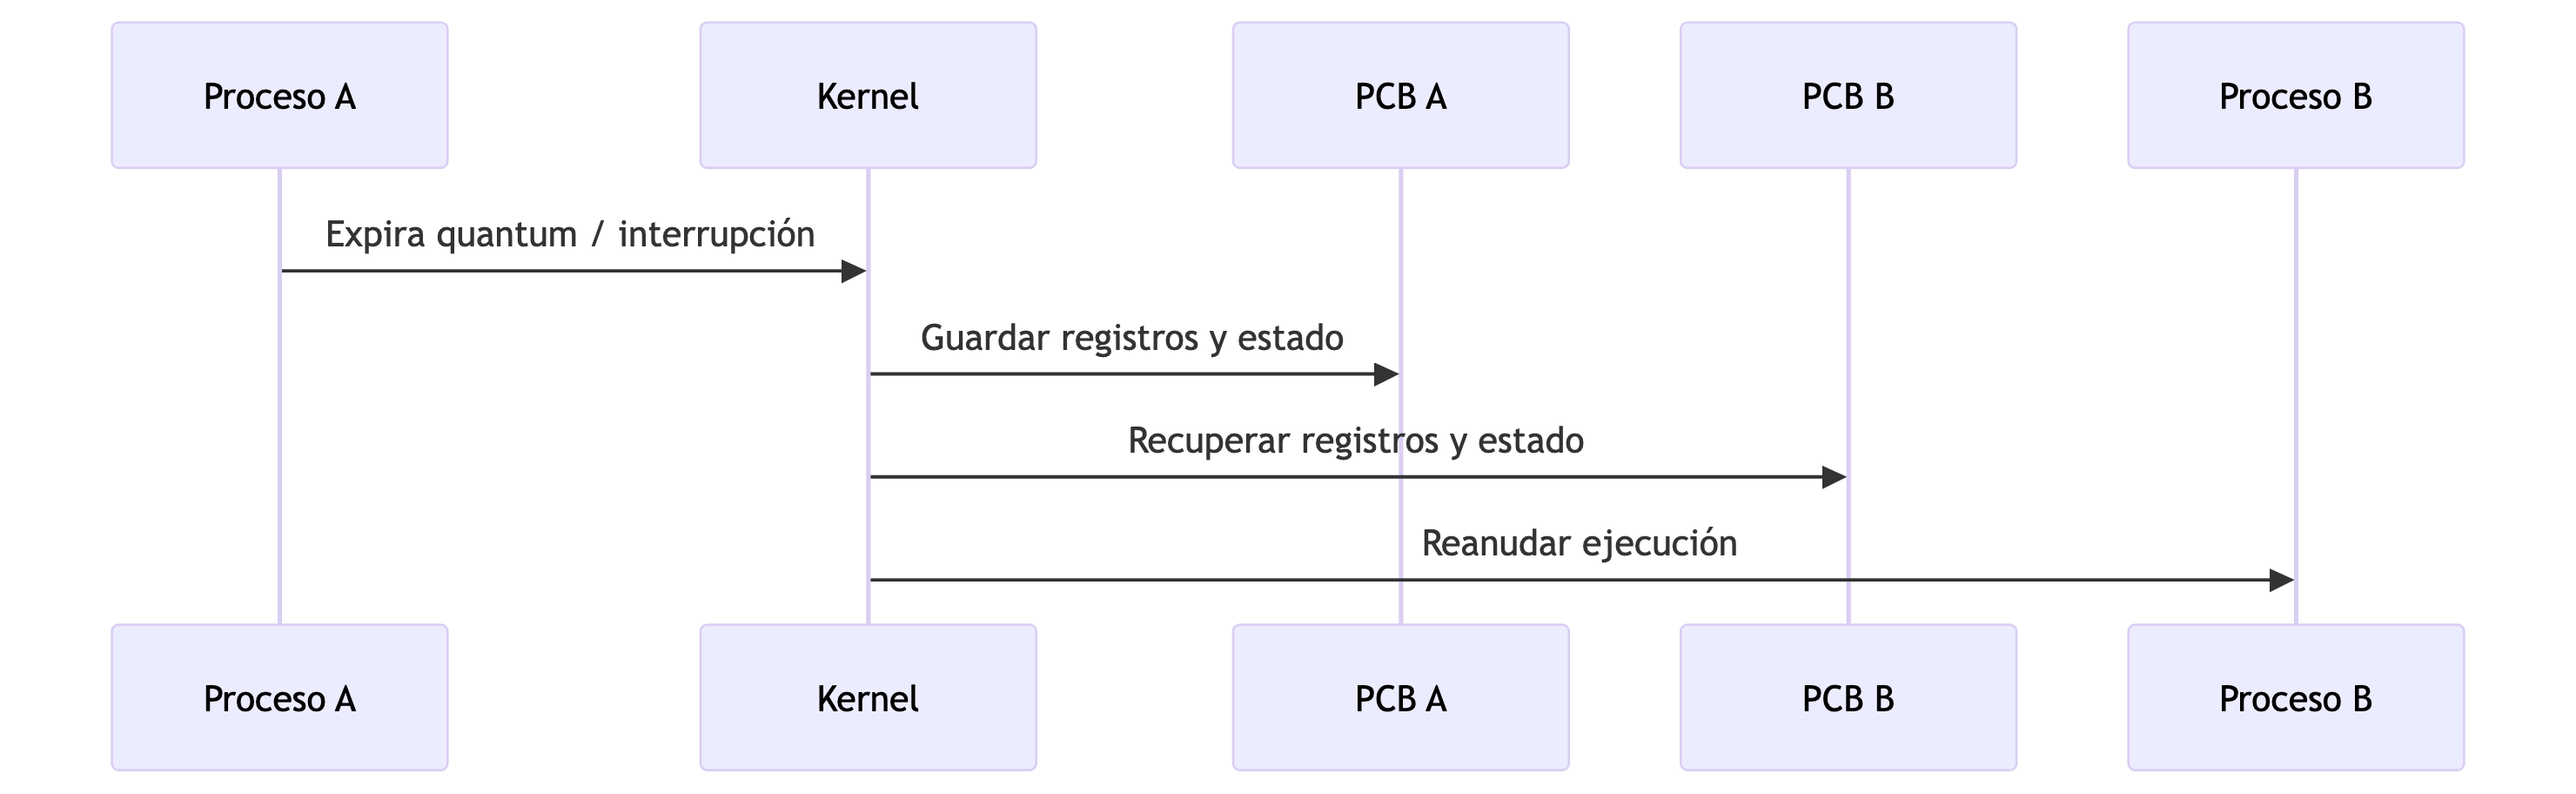
\includegraphics[width=6.2in,height=4.4in]{capitulos/05_control_procesos_concurrencia_files/figure-latex/mermaid-figure-6.png}

Un cambio de contexto tiene costo porque consume tiempo sin avanzar
directamente el trabajo de la aplicación. Sin embargo, es indispensable
para ofrecer multitarea, aislamiento y capacidad de respuesta.

\bookmarksetup{startatroot}

\chapter{Recursos compartidos}\label{recursos-compartidos}

La concurrencia se vuelve delicada cuando procesos o hilos acceden a un
mismo recurso.

Ejemplos:

\begin{itemize}
\tightlist
\item
  una variable;
\item
  un archivo;
\item
  una impresora;
\item
  una estructura en memoria;
\item
  un registro de base de datos;
\item
  una cola;
\item
  un dispositivo;
\item
  un contador.
\end{itemize}

\section{Ejemplo: contador
compartido}\label{ejemplo-contador-compartido}

Supongamos que:

\begin{Shaded}
\begin{Highlighting}[]
\NormalTok{contador = 10}
\end{Highlighting}
\end{Shaded}

Dos hilos ejecutan:

\begin{Shaded}
\begin{Highlighting}[]
\NormalTok{contador = contador + 1}
\end{Highlighting}
\end{Shaded}

La operación no siempre es indivisible. Puede implicar:

\begin{enumerate}
\def\labelenumi{\arabic{enumi}.}
\tightlist
\item
  leer contador;
\item
  sumar uno;
\item
  escribir el resultado.
\end{enumerate}

Posible intercalado:

{\def\LTcaptype{none} % do not increment counter
\begin{longtable}[]{@{}rllr@{}}
\toprule\noalign{}
Paso & Hilo A & Hilo B & Valor \\
\midrule\noalign{}
\endhead
\bottomrule\noalign{}
\endlastfoot
1 & Lee 10 & & 10 \\
2 & & Lee 10 & 10 \\
3 & Calcula 11 & & 10 \\
4 & & Calcula 11 & 10 \\
5 & Escribe 11 & & 11 \\
6 & & Escribe 11 & 11 \\
\end{longtable}
}

El resultado esperado era 12, pero se obtuvo 11.

\bookmarksetup{startatroot}

\chapter{Condición de carrera}\label{condiciuxf3n-de-carrera}

Una \textbf{condición de carrera} ocurre cuando el resultado depende del
orden o del momento en que varias unidades concurrentes acceden a datos
compartidos.

Sus características habituales son:

\begin{itemize}
\tightlist
\item
  es intermitente;
\item
  puede desaparecer al depurar;
\item
  depende de la planificación;
\item
  puede producir pérdida o corrupción de datos;
\item
  es difícil de reproducir;
\item
  puede convertirse en vulnerabilidad.
\end{itemize}

\begin{tcolorbox}[enhanced jigsaw, arc=.35mm, bottomrule=.15mm, bottomtitle=1mm, breakable, colback=white, colbacktitle=quarto-callout-warning-color!10!white, colframe=quarto-callout-warning-color-frame, coltitle=black, left=2mm, leftrule=.75mm, opacityback=0, opacitybacktitle=0.6, rightrule=.15mm, title=\textcolor{quarto-callout-warning-color}{\faExclamationTriangle}\hspace{0.5em}{Error común}, titlerule=0mm, toprule=.15mm, toptitle=1mm]

Concurrencia no significa automáticamente condición de carrera. El
problema aparece cuando existe acceso compartido sin una coordinación
correcta.

\end{tcolorbox}

\bookmarksetup{startatroot}

\chapter{Sección crítica}\label{secciuxf3n-cruxedtica}

Una \textbf{sección crítica} es la parte del programa que accede o
modifica un recurso compartido y que debe protegerse para evitar
interferencias.

\begin{Shaded}
\begin{Highlighting}[]
\NormalTok{Entrada a la sección crítica}

\NormalTok{    modificar recurso compartido}

\NormalTok{Salida de la sección crítica}
\end{Highlighting}
\end{Shaded}

Una solución correcta para la sección crítica busca cumplir:

\begin{enumerate}
\def\labelenumi{\arabic{enumi}.}
\tightlist
\item
  \textbf{Exclusión mutua:} solo una unidad entra a la vez.
\item
  \textbf{Progreso:} si nadie está dentro, debe poder seleccionarse
  quién entra.
\item
  \textbf{Espera limitada:} ninguna unidad debe esperar indefinidamente.
\end{enumerate}

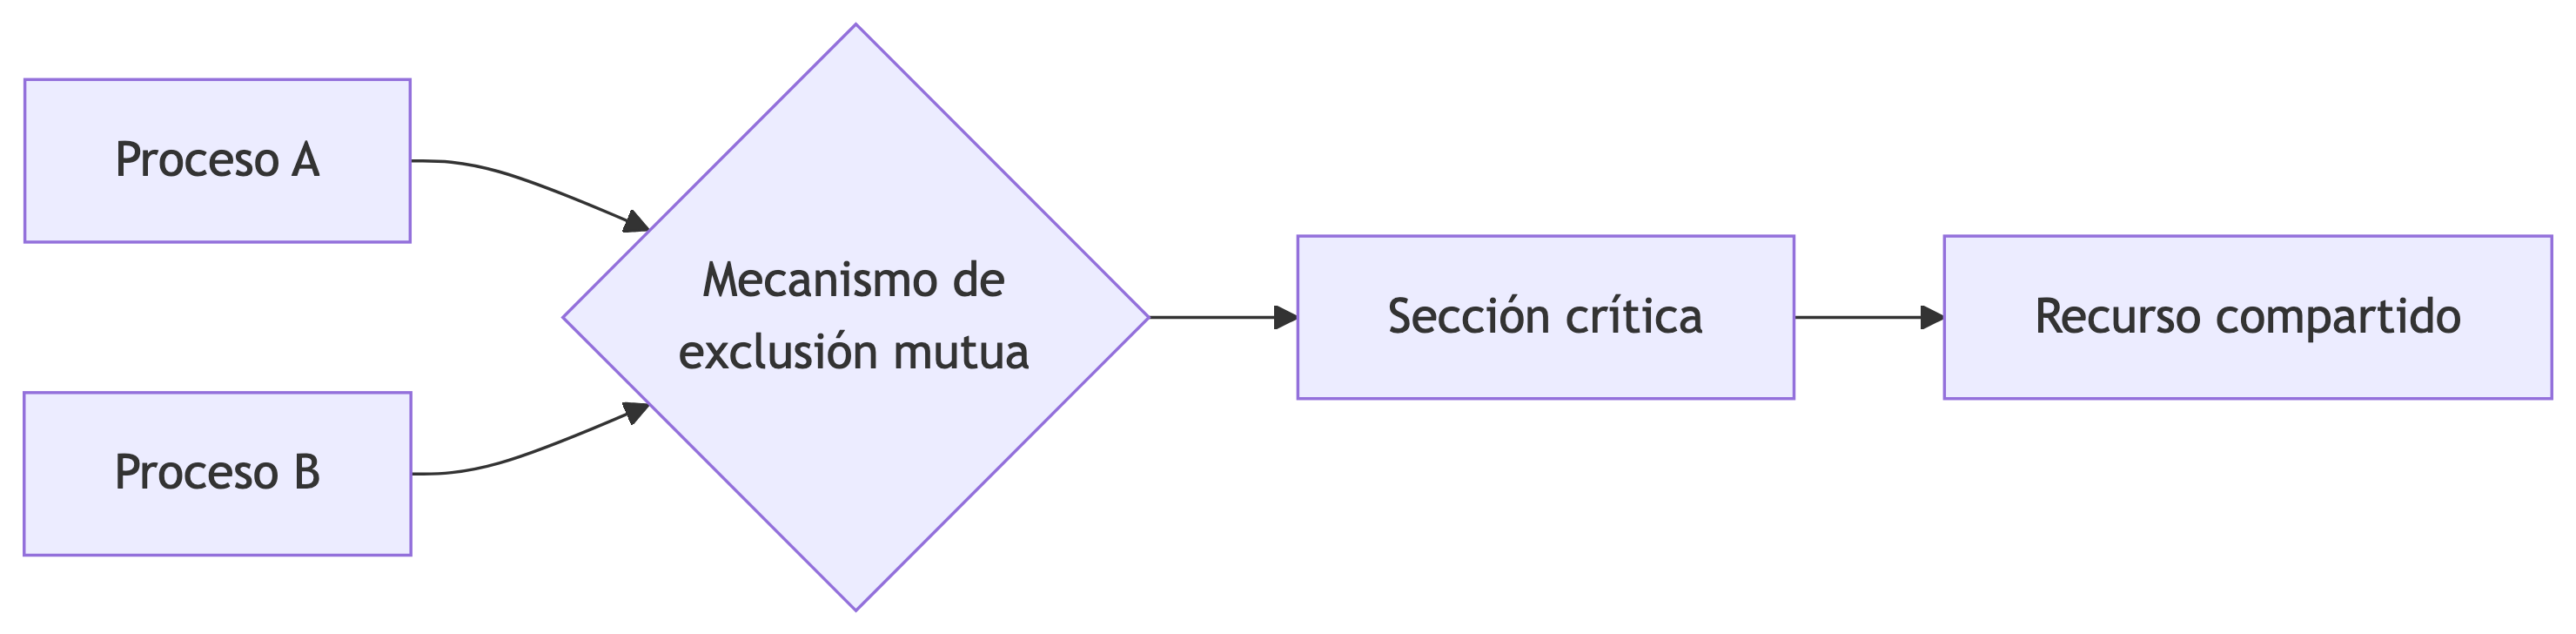
\includegraphics[width=6.2in,height=4in]{capitulos/05_control_procesos_concurrencia_files/figure-latex/mermaid-figure-5.png}

\bookmarksetup{startatroot}

\chapter{Mecanismos de
sincronización}\label{mecanismos-de-sincronizaciuxf3n}

Los sistemas modernos ofrecen mecanismos como:

{\def\LTcaptype{none} % do not increment counter
\begin{longtable}[]{@{}ll@{}}
\toprule\noalign{}
Mecanismo & Uso general \\
\midrule\noalign{}
\endhead
\bottomrule\noalign{}
\endlastfoot
Mutex & Exclusión mutua \\
Semáforo & Control de acceso y señalización \\
Monitor & Encapsulación de estado y sincronización \\
Variable de condición & Esperar hasta que ocurra una condición \\
Spinlock & Espera activa breve en contextos apropiados \\
Operación atómica & Actualización indivisible de datos simples \\
\end{longtable}
}

\begin{tcolorbox}[enhanced jigsaw, arc=.35mm, bottomrule=.15mm, bottomtitle=1mm, breakable, colback=white, colbacktitle=quarto-callout-important-color!10!white, colframe=quarto-callout-important-color-frame, coltitle=black, left=2mm, leftrule=.75mm, opacityback=0, opacitybacktitle=0.6, rightrule=.15mm, title=\textcolor{quarto-callout-important-color}{\faExclamation}\hspace{0.5em}{Criterio profesional}, titlerule=0mm, toprule=.15mm, toptitle=1mm]

No debe improvisarse un mecanismo de sincronización cuando el lenguaje o
el sistema operativo ya ofrece primitivas probadas.

\end{tcolorbox}

\bookmarksetup{startatroot}

\chapter{Algoritmo de Dekker}\label{algoritmo-de-dekker}

El \textbf{algoritmo de Dekker} es una solución histórica de software
para lograr exclusión mutua entre \textbf{dos procesos}.

Utiliza:

\begin{itemize}
\tightlist
\item
  una bandera por proceso;
\item
  una variable de turno;
\item
  espera activa.
\end{itemize}

\section{Idea general}\label{idea-general}

Cada proceso indica que desea entrar. Si ambos quieren entrar al mismo
tiempo, la variable \texttt{turno} resuelve quién cede temporalmente.

\section{Pseudocódigo conceptual}\label{pseudocuxf3digo-conceptual}

\begin{Shaded}
\begin{Highlighting}[]
\NormalTok{bandera[0] = falso}
\NormalTok{bandera[1] = falso}
\NormalTok{turno = 0}

\NormalTok{Proceso i:}
\NormalTok{    j = 1 {-} i}

\NormalTok{    mientras verdadero:}
\NormalTok{        bandera[i] = verdadero}

\NormalTok{        mientras bandera[j]:}
\NormalTok{            si turno == j:}
\NormalTok{                bandera[i] = falso}

\NormalTok{                mientras turno == j:}
\NormalTok{                    esperar}

\NormalTok{                bandera[i] = verdadero}

\NormalTok{        sección crítica}

\NormalTok{        turno = j}
\NormalTok{        bandera[i] = falso}

\NormalTok{        sección no crítica}
\end{Highlighting}
\end{Shaded}

\section{Explicación}\label{explicaciuxf3n}

\begin{enumerate}
\def\labelenumi{\arabic{enumi}.}
\tightlist
\item
  \texttt{bandera{[}i{]}\ =\ verdadero} anuncia intención de entrar.
\item
  Si el otro proceso no desea entrar, el proceso continúa.
\item
  Si ambos desean entrar, \texttt{turno} decide quién espera.
\item
  Al salir, se entrega el turno al otro proceso.
\item
  La bandera se desactiva.
\end{enumerate}

\begin{tcolorbox}[enhanced jigsaw, arc=.35mm, bottomrule=.15mm, bottomtitle=1mm, breakable, colback=white, colbacktitle=quarto-callout-note-color!10!white, colframe=quarto-callout-note-color-frame, coltitle=black, left=2mm, leftrule=.75mm, opacityback=0, opacitybacktitle=0.6, rightrule=.15mm, title=\textcolor{quarto-callout-note-color}{\faInfo}\hspace{0.5em}{Importancia histórica}, titlerule=0mm, toprule=.15mm, toptitle=1mm]

Dekker demuestra que la exclusión mutua puede lograrse mediante
coordinación lógica entre dos procesos.

\end{tcolorbox}

\begin{tcolorbox}[enhanced jigsaw, arc=.35mm, bottomrule=.15mm, bottomtitle=1mm, breakable, colback=white, colbacktitle=quarto-callout-warning-color!10!white, colframe=quarto-callout-warning-color-frame, coltitle=black, left=2mm, leftrule=.75mm, opacityback=0, opacitybacktitle=0.6, rightrule=.15mm, title=\textcolor{quarto-callout-warning-color}{\faExclamationTriangle}\hspace{0.5em}{Limitación práctica}, titlerule=0mm, toprule=.15mm, toptitle=1mm]

Dekker es valioso para estudiar concurrencia, pero no debe implementarse
como sustituto de mutex, semáforos u operaciones atómicas en
aplicaciones modernas. Además, los modelos modernos de memoria y las
optimizaciones del compilador requieren primitivas con garantías
explícitas.

\end{tcolorbox}

\bookmarksetup{startatroot}

\chapter{Interbloqueo, inanición y
livelock}\label{interbloqueo-inaniciuxf3n-y-livelock}

Estos problemas no son iguales.

{\def\LTcaptype{none} % do not increment counter
\begin{longtable}[]{@{}
  >{\raggedright\arraybackslash}p{(\linewidth - 2\tabcolsep) * \real{0.5000}}
  >{\raggedright\arraybackslash}p{(\linewidth - 2\tabcolsep) * \real{0.5000}}@{}}
\toprule\noalign{}
\begin{minipage}[b]{\linewidth}\raggedright
Problema
\end{minipage} & \begin{minipage}[b]{\linewidth}\raggedright
Descripción
\end{minipage} \\
\midrule\noalign{}
\endhead
\bottomrule\noalign{}
\endlastfoot
Interbloqueo & Dos o más procesos esperan recursos retenidos entre sí \\
Inanición & Un proceso espera indefinidamente porque otros reciben
preferencia \\
Livelock & Los procesos cambian de estado, pero no progresan \\
Condición de carrera & El resultado depende del intercalado no
controlado \\
\end{longtable}
}

\section{Ejemplo de interbloqueo}\label{ejemplo-de-interbloqueo}

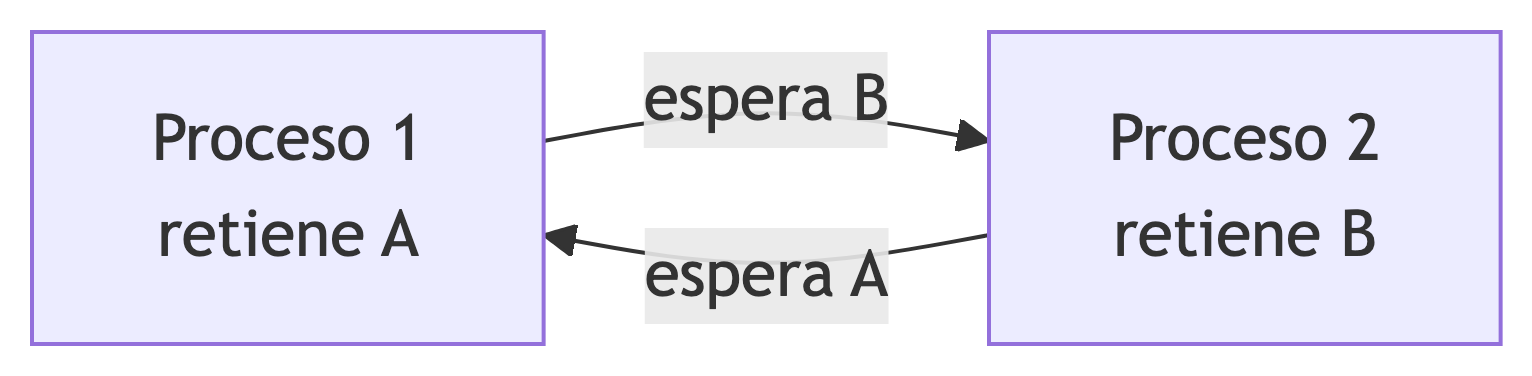
\includegraphics[width=5.8in,height=3.8in]{capitulos/05_control_procesos_concurrencia_files/figure-latex/mermaid-figure-4.png}

\bookmarksetup{startatroot}

\chapter{Inteligencia artificial y control de
procesos}\label{inteligencia-artificial-y-control-de-procesos}

La IA puede utilizarse para analizar métricas y apoyar políticas de
administración. Sin embargo, debe distinguirse entre:

\begin{itemize}
\tightlist
\item
  funciones presentes en sistemas de producción;
\item
  mecanismos experimentales;
\item
  investigación académica;
\item
  posibilidades futuras.
\end{itemize}

\begin{tcolorbox}[enhanced jigsaw, arc=.35mm, bottomrule=.15mm, bottomtitle=1mm, breakable, colback=white, colbacktitle=quarto-callout-important-color!10!white, colframe=quarto-callout-important-color-frame, coltitle=black, left=2mm, leftrule=.75mm, opacityback=0, opacitybacktitle=0.6, rightrule=.15mm, title=\textcolor{quarto-callout-important-color}{\faExclamation}\hspace{0.5em}{Aclaración}, titlerule=0mm, toprule=.15mm, toptitle=1mm]

La IA no ``entra al PCB'' ni sustituye las estructuras del kernel. Un
modelo puede analizar información derivada de procesos y recomendar o
ejecutar decisiones mediante interfaces controladas.

\end{tcolorbox}

\section{Áreas de aplicación}\label{uxe1reas-de-aplicaciuxf3n}

\subsection{Predicción de carga}\label{predicciuxf3n-de-carga}

Un modelo puede estimar:

\begin{itemize}
\tightlist
\item
  consumo futuro de CPU;
\item
  presión de memoria;
\item
  comportamiento interactivo;
\item
  ráfagas de entrada/salida;
\item
  demanda de energía.
\end{itemize}

\subsection{Planificación adaptativa}\label{planificaciuxf3n-adaptativa}

La investigación explora planificadores capaces de ajustar políticas
según:

\begin{itemize}
\tightlist
\item
  tipo de carga;
\item
  latencia;
\item
  rendimiento;
\item
  consumo energético;
\item
  afinidad entre tareas y núcleos;
\item
  objetivos de servicio.
\end{itemize}

\subsection{Detección de anomalías}\label{detecciuxf3n-de-anomaluxedas}

Los datos de procesos pueden utilizarse para detectar:

\begin{itemize}
\tightlist
\item
  consumo inusual;
\item
  procesos que dejan de responder;
\item
  fugas de memoria;
\item
  patrones sospechosos;
\item
  degradación de rendimiento.
\end{itemize}

\subsection{Administración
energética}\label{administraciuxf3n-energuxe9tica}

En equipos móviles, servidores y centros de datos, modelos predictivos
pueden apoyar decisiones sobre:

\begin{itemize}
\tightlist
\item
  frecuencias;
\item
  núcleos activos;
\item
  distribución de carga;
\item
  consolidación de tareas;
\item
  límites térmicos.
\end{itemize}

\bookmarksetup{startatroot}

\chapter{IA, PCB y Scheduler: relación
correcta}\label{ia-pcb-y-scheduler-relaciuxf3n-correcta}

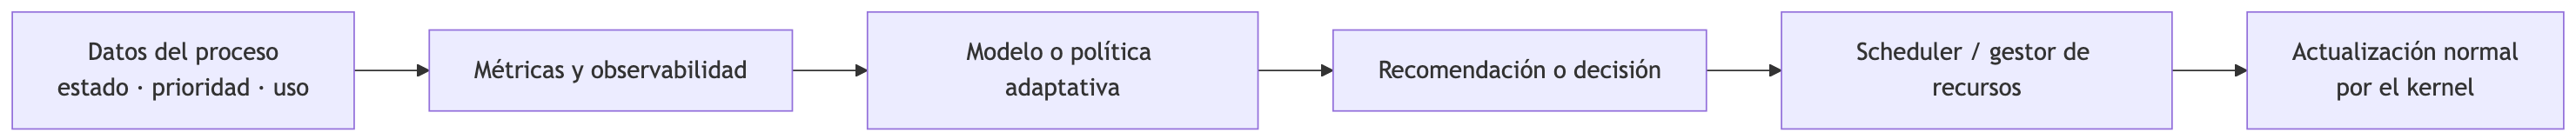
\includegraphics[width=6.2in,height=4.6in]{capitulos/05_control_procesos_concurrencia_files/figure-latex/mermaid-figure-3.png}

La secuencia correcta es:

\begin{enumerate}
\def\labelenumi{\arabic{enumi}.}
\tightlist
\item
  El kernel conserva y actualiza las estructuras del proceso.
\item
  Herramientas de observabilidad obtienen métricas.
\item
  Un modelo puede analizar esas métricas.
\item
  La política entrega una decisión a través de una interfaz válida.
\item
  El sistema operativo aplica la decisión y actualiza sus estructuras.
\end{enumerate}

\section{Estado actual: planificadores
extensibles}\label{estado-actual-planificadores-extensibles}

Linux dispone de \texttt{sched\_ext}, una clase de planificación
extensible basada en BPF que permite experimentar con algoritmos de
planificación externos y regresar al planificador predeterminado cuando
se detectan errores. Esta interfaz permite investigar políticas
personalizadas, incluidas políticas que podrían integrar modelos
predictivos, pero no implica que los sistemas operativos de escritorio
utilicen IA de manera general para reemplazar su Scheduler.
\href{https://docs.kernel.org/scheduler/sched-ext.html}{Documentación
oficial del kernel de Linux}.

\begin{tcolorbox}[enhanced jigsaw, arc=.35mm, bottomrule=.15mm, bottomtitle=1mm, breakable, colback=white, colbacktitle=quarto-callout-warning-color!10!white, colframe=quarto-callout-warning-color-frame, coltitle=black, left=2mm, leftrule=.75mm, opacityback=0, opacitybacktitle=0.6, rightrule=.15mm, title=\textcolor{quarto-callout-warning-color}{\faExclamationTriangle}\hspace{0.5em}{No confundir posibilidad con adopción}, titlerule=0mm, toprule=.15mm, toptitle=1mm]

Que una interfaz permita implementar una política inteligente no
significa que todo sistema operativo actual utilice aprendizaje
automático para planificar procesos.

\end{tcolorbox}

\bookmarksetup{startatroot}

\chapter{Comparación: planificación clásica y
adaptativa}\label{comparaciuxf3n-planificaciuxf3n-cluxe1sica-y-adaptativa}

{\def\LTcaptype{none} % do not increment counter
\begin{longtable}[]{@{}
  >{\raggedright\arraybackslash}p{(\linewidth - 4\tabcolsep) * \real{0.3333}}
  >{\raggedright\arraybackslash}p{(\linewidth - 4\tabcolsep) * \real{0.3333}}
  >{\raggedright\arraybackslash}p{(\linewidth - 4\tabcolsep) * \real{0.3333}}@{}}
\toprule\noalign{}
\begin{minipage}[b]{\linewidth}\raggedright
Aspecto
\end{minipage} & \begin{minipage}[b]{\linewidth}\raggedright
Planificación clásica
\end{minipage} & \begin{minipage}[b]{\linewidth}\raggedright
Enfoque adaptativo o basado en datos
\end{minipage} \\
\midrule\noalign{}
\endhead
\bottomrule\noalign{}
\endlastfoot
Reglas & Definidas previamente & Ajustadas según métricas o
predicciones \\
Interpretación & Generalmente clara & Puede ser más compleja \\
Costo & Predecible & Incluye inferencia y recolección de datos \\
Verificación & Más directa & Requiere validar modelo y política \\
Robustez & Amplia experiencia acumulada & Depende de entrenamiento y
límites \\
Uso & Generalizado & Investigación y escenarios especializados \\
\end{longtable}
}

\bookmarksetup{startatroot}

\chapter{Caso integrador: navegador durante una
videoclase}\label{caso-integrador-navegador-durante-una-videoclase}

Un estudiante participa en una videoclase mientras:

\begin{itemize}
\tightlist
\item
  reproduce audio y video;
\item
  escribe en el chat;
\item
  descarga un documento;
\item
  mantiene varias pestañas;
\item
  guarda apuntes;
\item
  recibe notificaciones.
\end{itemize}

\section{Análisis}\label{anuxe1lisis}

\begin{enumerate}
\def\labelenumi{\arabic{enumi}.}
\tightlist
\item
  El navegador puede utilizar varios procesos e hilos.
\item
  El Scheduler distribuye tiempo de CPU.
\item
  Cada hilo conserva su contexto de ejecución.
\item
  Las operaciones de red o disco pueden bloquear temporalmente tareas.
\item
  Al expirar el quantum, una tarea puede volver a READY.
\item
  Los buffers y estructuras compartidas requieren sincronización.
\item
  Una condición de carrera podría corromper datos.
\item
  Los mutex y otras primitivas protegen secciones críticas.
\item
  Herramientas de observabilidad pueden detectar consumo anómalo.
\item
  Una política adaptativa podría ajustar prioridades, pero el kernel
  conserva el control.
\end{enumerate}

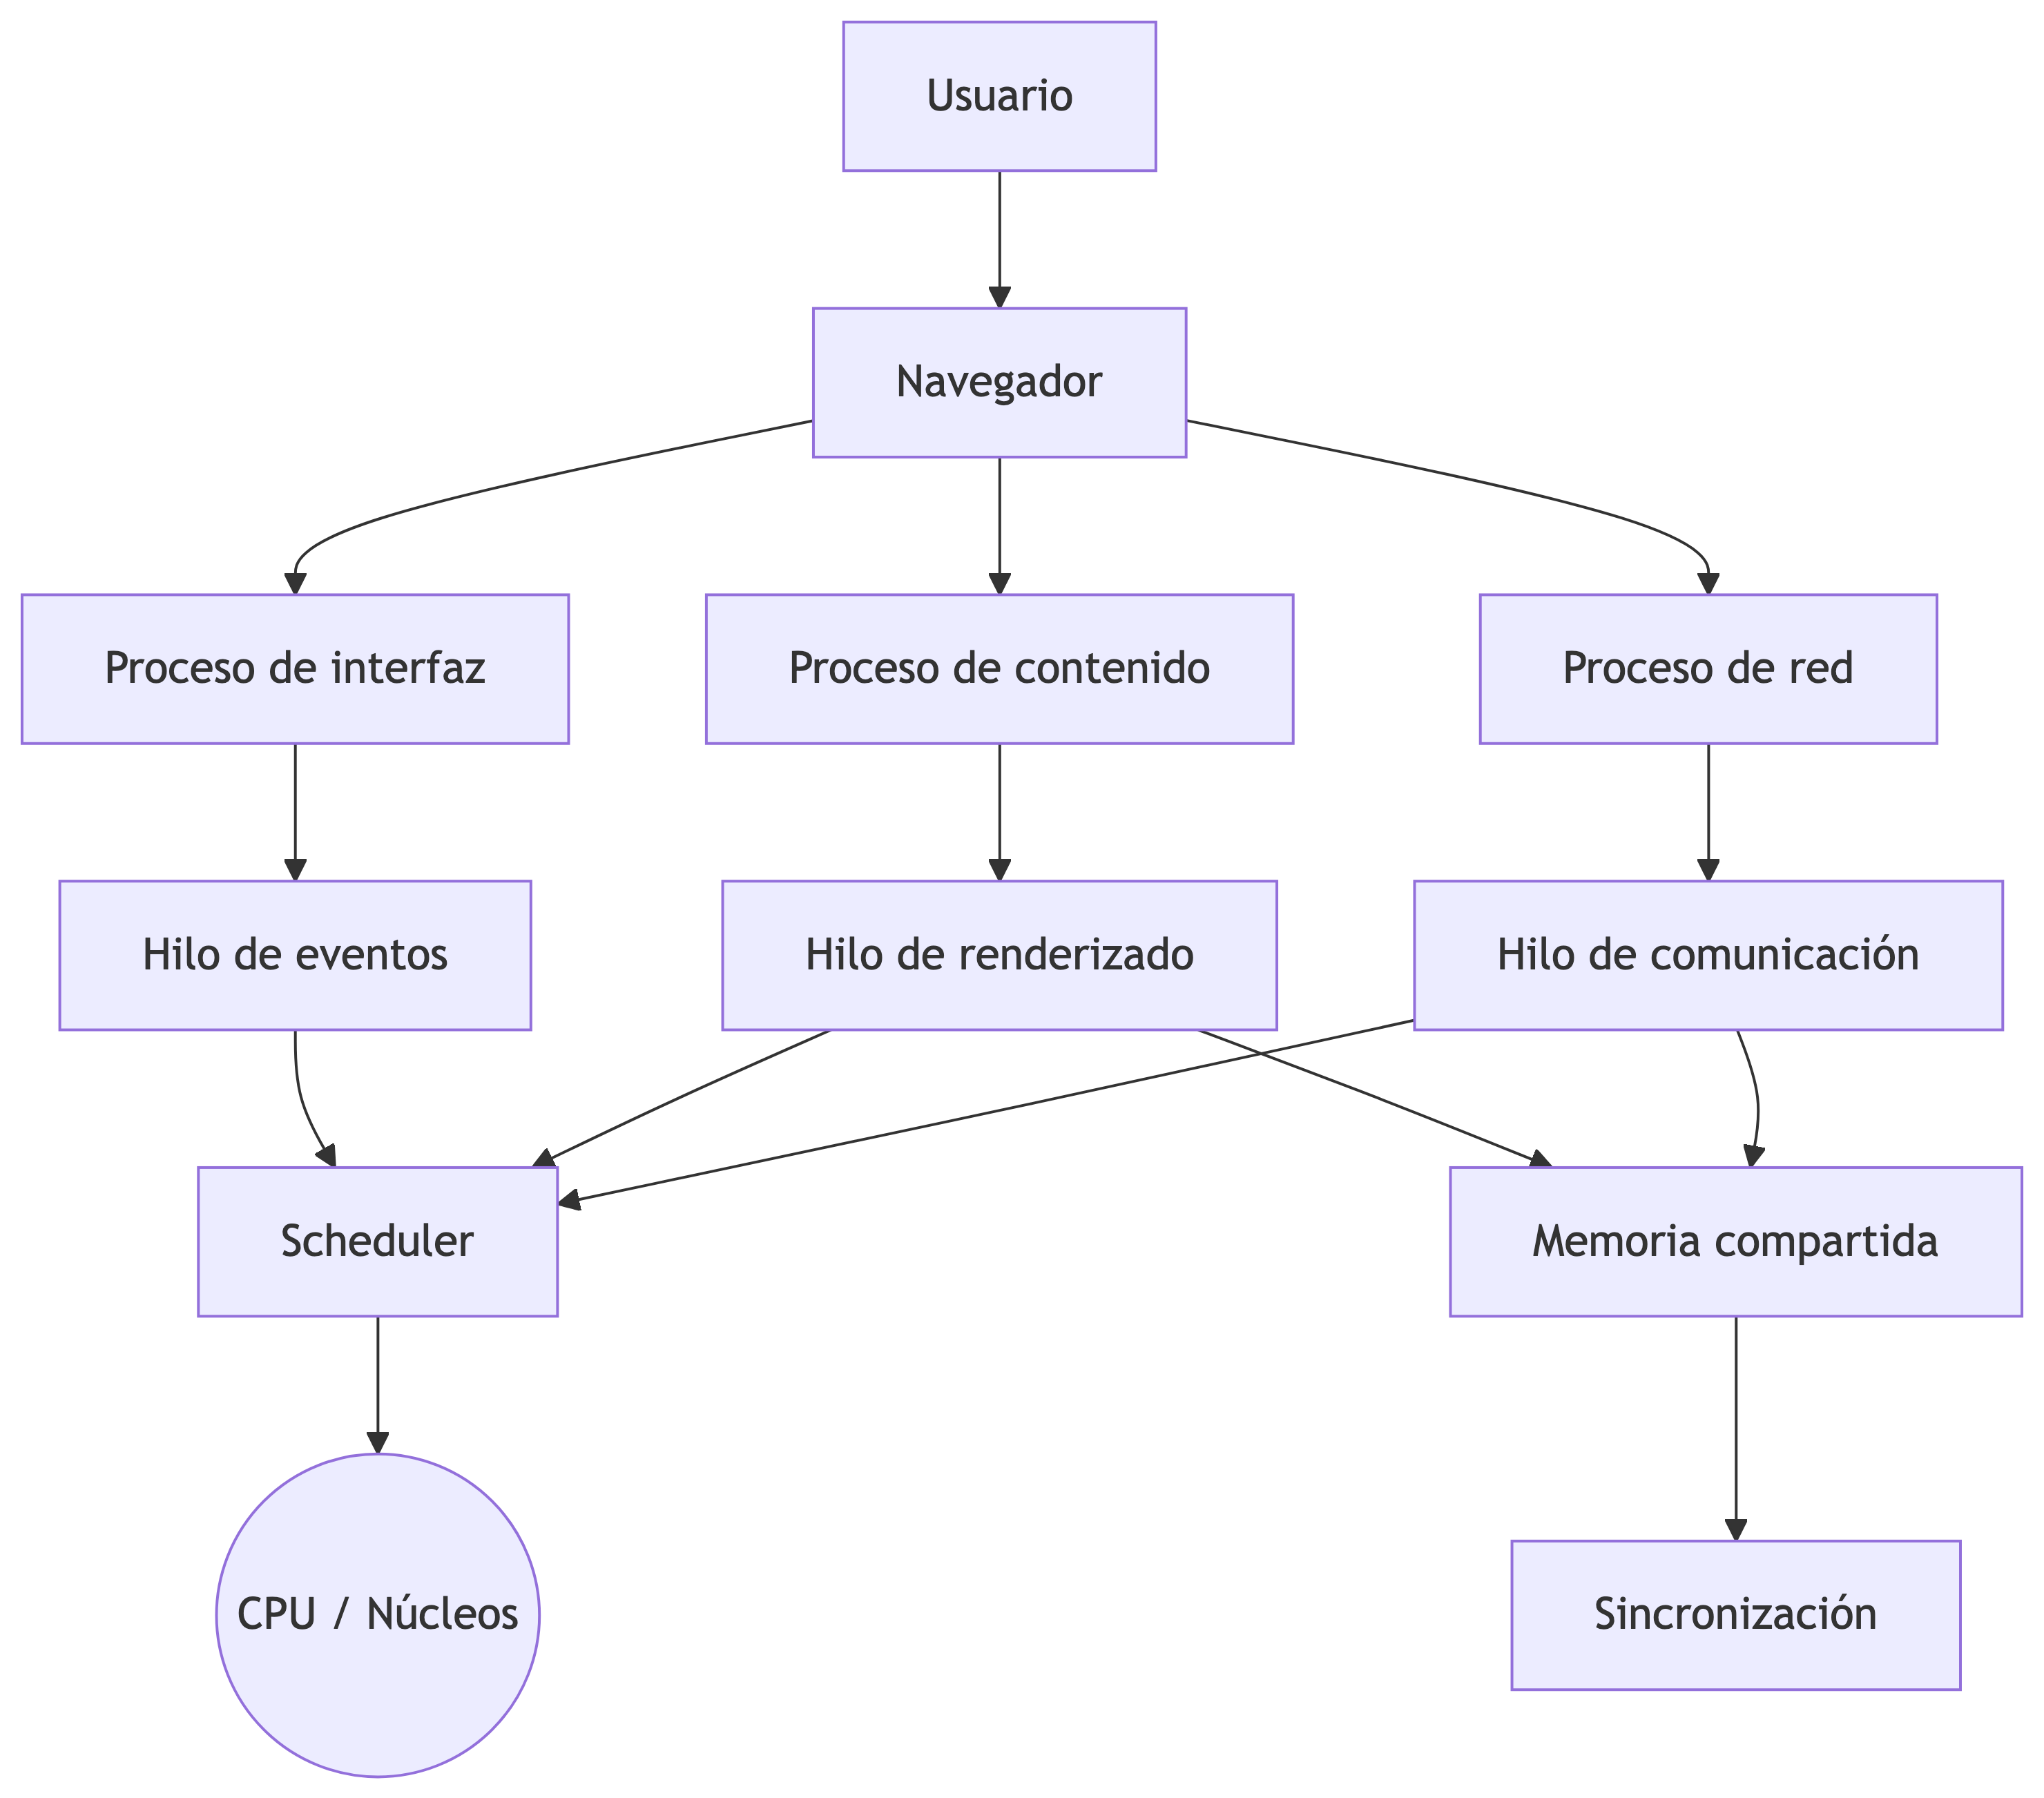
\includegraphics[width=6.2in,height=5.4in]{capitulos/05_control_procesos_concurrencia_files/figure-latex/mermaid-figure-2.png}

\bookmarksetup{startatroot}

\chapter{Laboratorio: observando procesos e
hilos}\label{laboratorio-observando-procesos-e-hilos}

\section{Propósito}\label{propuxf3sito-1}

Relacionar los conceptos de procesos, hilos, estados, CPU y cambios de
contexto con información real del sistema.

\section{Parte A. Windows}\label{parte-a.-windows}

Abra \textbf{Administrador de tareas} o \textbf{Monitor de recursos}.

Registre:

{\def\LTcaptype{none} % do not increment counter
\begin{longtable}[]{@{}ll@{}}
\toprule\noalign{}
Elemento & Resultado \\
\midrule\noalign{}
\endhead
\bottomrule\noalign{}
\endlastfoot
Proceso con mayor uso de CPU & \\
Proceso con mayor uso de memoria & \\
Número aproximado de procesos & \\
Número aproximado de hilos & \\
Aplicación con varios procesos relacionados & \\
\end{longtable}
}

Opcionalmente, en PowerShell:

\begin{Shaded}
\begin{Highlighting}[]
\FunctionTok{Get{-}Process} \OperatorTok{|}
  \FunctionTok{Sort{-}Object}\NormalTok{ CPU }\OperatorTok{{-}}\NormalTok{Descending }\OperatorTok{|}
  \FunctionTok{Select{-}Object} \OperatorTok{{-}}\NormalTok{First }\DecValTok{10}\NormalTok{ Name}\OperatorTok{,}\NormalTok{ Id}\OperatorTok{,}\NormalTok{ CPU}\OperatorTok{,}\NormalTok{ Threads}\OperatorTok{,}\NormalTok{ WorkingSet}
\end{Highlighting}
\end{Shaded}

\section{Parte B. macOS}\label{parte-b.-macos}

Abra \textbf{Monitor de Actividad}.

También puede utilizar:

\begin{Shaded}
\begin{Highlighting}[]
\FunctionTok{ps} \AttributeTok{{-}axo}\NormalTok{ pid,ppid,state,\%cpu,\%mem,comm }\KeywordTok{|} \FunctionTok{head}
\end{Highlighting}
\end{Shaded}

y:

\begin{Shaded}
\begin{Highlighting}[]
\ExtensionTok{top} \AttributeTok{{-}l}\NormalTok{ 1 }\AttributeTok{{-}stats}\NormalTok{ pid,command,cpu,mem,threads}
\end{Highlighting}
\end{Shaded}

\section{Parte C. GNU/Linux}\label{parte-c.-gnulinux}

Utilice:

\begin{Shaded}
\begin{Highlighting}[]
\FunctionTok{ps} \AttributeTok{{-}eo}\NormalTok{ pid,ppid,stat,pri,ni,\%cpu,\%mem,comm }\AttributeTok{{-}{-}sort}\OperatorTok{=}\NormalTok{{-}\%cpu }\KeywordTok{|} \FunctionTok{head}
\end{Highlighting}
\end{Shaded}

Para observar hilos:

\begin{Shaded}
\begin{Highlighting}[]
\FunctionTok{ps} \AttributeTok{{-}eLf} \KeywordTok{|} \FunctionTok{head}
\end{Highlighting}
\end{Shaded}

También puede utilizar:

\begin{Shaded}
\begin{Highlighting}[]
\ExtensionTok{top}
\end{Highlighting}
\end{Shaded}

o, si está instalado:

\begin{Shaded}
\begin{Highlighting}[]
\ExtensionTok{htop}
\end{Highlighting}
\end{Shaded}

\begin{tcolorbox}[enhanced jigsaw, arc=.35mm, bottomrule=.15mm, bottomtitle=1mm, breakable, colback=white, colbacktitle=quarto-callout-warning-color!10!white, colframe=quarto-callout-warning-color-frame, coltitle=black, left=2mm, leftrule=.75mm, opacityback=0, opacitybacktitle=0.6, rightrule=.15mm, title=\textcolor{quarto-callout-warning-color}{\faExclamationTriangle}\hspace{0.5em}{Regla de seguridad del laboratorio}, titlerule=0mm, toprule=.15mm, toptitle=1mm]

La actividad es únicamente de observación. No finalice procesos del
sistema, no cambie prioridades y no ejecute comandos con privilegios
administrativos.

\end{tcolorbox}

\section{Preguntas de análisis}\label{preguntas-de-anuxe1lisis}

\begin{enumerate}
\def\labelenumi{\arabic{enumi}.}
\tightlist
\item
  ¿Qué diferencia observa entre proceso e hilo?
\item
  ¿Qué proceso tiene más hilos?
\item
  ¿El proceso con mayor memoria también utiliza más CPU?
\item
  ¿Qué significan los estados observados?
\item
  ¿Por qué el uso de CPU cambia constantemente?
\item
  ¿Qué aplicación parece utilizar una arquitectura multiproceso?
\item
  ¿Qué riesgo tendría finalizar un proceso sin conocer su función?
\end{enumerate}

\bookmarksetup{startatroot}

\chapter{Actividad en clase: simulación de Round
Robin}\label{actividad-en-clase-simulaciuxf3n-de-round-robin}

\section{Materiales}\label{materiales}

\begin{itemize}
\tightlist
\item
  Cuatro tarjetas de procesos.
\item
  Un cronómetro.
\item
  Una tabla de seguimiento.
\end{itemize}

\section{Datos}\label{datos}

{\def\LTcaptype{none} % do not increment counter
\begin{longtable}[]{@{}lr@{}}
\toprule\noalign{}
Proceso & Ráfaga \\
\midrule\noalign{}
\endhead
\bottomrule\noalign{}
\endlastfoot
P1 & 7 \\
P2 & 4 \\
P3 & 9 \\
P4 & 5 \\
\end{longtable}
}

Use:

\begin{Shaded}
\begin{Highlighting}[]
\NormalTok{Quantum = 3}
\end{Highlighting}
\end{Shaded}

\section{Instrucciones}\label{instrucciones}

\begin{enumerate}
\def\labelenumi{\arabic{enumi}.}
\tightlist
\item
  Coloque los procesos en la cola.
\item
  Asigne tres unidades al primero.
\item
  Si no termina, envíelo al final.
\item
  Registre cada cambio.
\item
  Calcule el tiempo de finalización.
\item
  Cuente los cambios de contexto.
\item
  Repita con quantum 1 y quantum 6.
\item
  Compare los resultados.
\end{enumerate}

\section{Tabla de resultados}\label{tabla-de-resultados}

{\def\LTcaptype{none} % do not increment counter
\begin{longtable}[]{@{}rrll@{}}
\toprule\noalign{}
Quantum & Cambios de contexto & Respuesta percibida & Observación \\
\midrule\noalign{}
\endhead
\bottomrule\noalign{}
\endlastfoot
1 & & & \\
3 & & & \\
6 & & & \\
\end{longtable}
}

\bookmarksetup{startatroot}

\chapter{Reto del Ingeniero}\label{reto-del-ingeniero-1}

Una aplicación bancaria ejecuta varios hilos:

\begin{itemize}
\tightlist
\item
  interfaz;
\item
  validación;
\item
  consulta de saldo;
\item
  registro de transacciones;
\item
  generación de comprobantes.
\end{itemize}

Dos hilos actualizan simultáneamente el saldo de una cuenta.

Responda:

\begin{enumerate}
\def\labelenumi{\arabic{enumi}.}
\tightlist
\item
  ¿Cuál es el recurso compartido?
\item
  ¿Dónde existe una sección crítica?
\item
  ¿Qué condición de carrera podría ocurrir?
\item
  ¿Qué mecanismo de sincronización propondría?
\item
  ¿Qué información del proceso conservaría el sistema operativo?
\item
  ¿Qué métricas permitirían detectar comportamiento anómalo?
\item
  ¿Qué decisión nunca debería dejarse únicamente a un modelo de IA sin
  controles?
\end{enumerate}

\bookmarksetup{startatroot}

\chapter{Autoevaluación}\label{autoevaluaciuxf3n-2}

\section{Selección múltiple}\label{selecciuxf3n-muxfaltiple}

\begin{enumerate}
\def\labelenumi{\arabic{enumi}.}
\item
  ¿Qué comparte normalmente un grupo de hilos del mismo proceso?

  \begin{enumerate}
  \def\labelenumii{\alph{enumii}.}
  \tightlist
  \item
    Únicamente el PID\\
  \item
    Espacio de direcciones y recursos\\
  \item
    Ningún recurso\\
  \item
    Procesadores físicos
  \end{enumerate}
\item
  ¿Qué ocurre cuando expira el quantum?

  \begin{enumerate}
  \def\labelenumii{\alph{enumii}.}
  \tightlist
  \item
    El proceso siempre termina\\
  \item
    El proceso se elimina\\
  \item
    El kernel puede interrumpirlo y devolverlo a READY\\
  \item
    Se borra su PCB
  \end{enumerate}
\item
  ¿Qué caracteriza una condición de carrera?

  \begin{enumerate}
  \def\labelenumii{\alph{enumii}.}
  \tightlist
  \item
    El resultado depende del intercalado\\
  \item
    Todos los procesos terminan en orden\\
  \item
    No existen recursos compartidos\\
  \item
    El quantum es demasiado grande
  \end{enumerate}
\item
  ¿Qué busca garantizar un mutex?

  \begin{enumerate}
  \def\labelenumii{\alph{enumii}.}
  \tightlist
  \item
    Paralelismo ilimitado\\
  \item
    Exclusión mutua\\
  \item
    Eliminación del PCB\\
  \item
    Mayor memoria RAM
  \end{enumerate}
\item
  ¿Para cuántos procesos fue diseñado Dekker?

  \begin{enumerate}
  \def\labelenumii{\alph{enumii}.}
  \tightlist
  \item
    Uno\\
  \item
    Dos\\
  \item
    Diez\\
  \item
    Un número ilimitado
  \end{enumerate}
\item
  ¿Cuál afirmación sobre IA y PCB es más precisa?

  \begin{enumerate}
  \def\labelenumii{\alph{enumii}.}
  \tightlist
  \item
    La IA reemplaza siempre el PCB\\
  \item
    La IA modifica directamente cualquier estructura del kernel\\
  \item
    Un modelo puede apoyar decisiones utilizando métricas observadas\\
  \item
    Todo sistema operativo utiliza redes neuronales
  \end{enumerate}
\end{enumerate}

\begin{tcolorbox}[enhanced jigsaw, arc=.35mm, bottomrule=.15mm, bottomtitle=1mm, breakable, colback=white, colbacktitle=quarto-callout-note-color!10!white, colframe=quarto-callout-note-color-frame, coltitle=black, left=2mm, leftrule=.75mm, opacityback=0, opacitybacktitle=0.6, rightrule=.15mm, title=\textcolor{quarto-callout-note-color}{\faInfo}\hspace{0.5em}{Respuestas}, titlerule=0mm, toprule=.15mm, toptitle=1mm]

\begin{enumerate}
\def\labelenumi{\arabic{enumi}.}
\tightlist
\item
  b\\
\item
  c\\
\item
  a\\
\item
  b\\
\item
  b\\
\item
  c
\end{enumerate}

\end{tcolorbox}

\section{Preguntas de reflexión}\label{preguntas-de-reflexiuxf3n-1}

\begin{enumerate}
\def\labelenumi{\arabic{enumi}.}
\tightlist
\item
  ¿Por qué un quantum demasiado pequeño puede reducir el rendimiento?
\item
  ¿Cuál es la diferencia entre concurrencia y paralelismo?
\item
  ¿Por qué los hilos son más ligeros, pero también menos aislados?
\item
  ¿Por qué una condición de carrera puede ser difícil de reproducir?
\item
  ¿Qué valor educativo tiene Dekker aunque no sea la opción usual en
  aplicaciones modernas?
\item
  ¿Qué riesgos introduce una política de planificación basada en
  aprendizaje automático?
\end{enumerate}

\bookmarksetup{startatroot}

\chapter{Resumen de la clase}\label{resumen-de-la-clase-3}

En esta clase aprendimos que:

\begin{itemize}
\tightlist
\item
  El control de procesos abarca creación, planificación, sincronización
  y finalización.
\item
  Un proceso posee recursos propios y puede contener varios hilos.
\item
  La concurrencia permite que varias tareas progresen durante un mismo
  período.
\item
  El paralelismo requiere ejecución simultánea en hardware distinto.
\item
  El quantum limita temporalmente el uso de CPU.
\item
  Round Robin distribuye turnos entre los procesos listos.
\item
  El PCB conserva la información necesaria para administrar un proceso.
\item
  Los cambios de contexto permiten alternar entre unidades de ejecución.
\item
  Los recursos compartidos pueden producir condiciones de carrera.
\item
  Las secciones críticas deben protegerse mediante sincronización.
\item
  Dekker es una solución histórica para dos procesos.
\item
  La IA puede apoyar predicción, observabilidad y políticas adaptativas,
  pero no reemplaza automáticamente al kernel.
\end{itemize}

\begin{tcolorbox}[enhanced jigsaw, arc=.35mm, bottomrule=.15mm, bottomtitle=1mm, breakable, colback=white, colbacktitle=quarto-callout-tip-color!10!white, colframe=quarto-callout-tip-color-frame, coltitle=black, left=2mm, leftrule=.75mm, opacityback=0, opacitybacktitle=0.6, rightrule=.15mm, title=\textcolor{quarto-callout-tip-color}{\faLightbulb}\hspace{0.5em}{Consejo final del Ingeniero}, titlerule=0mm, toprule=.15mm, toptitle=1mm]

La concurrencia no se domina memorizando nombres. Se comprende siguiendo
el orden exacto de las operaciones y preguntando qué datos comparten las
unidades de ejecución.

\end{tcolorbox}

\bookmarksetup{startatroot}

\chapter{Tarea sugerida}\label{tarea-sugerida-2}

\begin{enumerate}
\def\labelenumi{\arabic{enumi}.}
\tightlist
\item
  Dibuje el modelo de cinco estados.
\item
  Dibuje y explique los componentes principales del PCB.
\item
  Resuelva manualmente un ejercicio Round Robin con cuatro procesos.
\item
  Describa una condición de carrera de la vida real.
\item
  Compare mutex, semáforo y monitor.
\item
  Explique el algoritmo de Dekker con sus propias palabras.
\item
  Redacte una conclusión sobre el uso responsable de IA en la
  planificación de procesos.
\end{enumerate}

\bookmarksetup{startatroot}

\chapter{Referencias y
actualización}\label{referencias-y-actualizaciuxf3n}

\begin{itemize}
\tightlist
\item
  Material base de la Clase 5: \emph{Control de Procesos y
  Concurrencia}. fileciteturn8file0
\item
  Linux Kernel Documentation. \emph{Extensible Scheduler Class
  (sched\_ext)}.
\item
  Silberschatz, A., Galvin, P. B., \& Gagne, G. \emph{Operating System
  Concepts}.
\item
  Stallings, W. \emph{Operating Systems: Internals and Design
  Principles}.
\item
  Tanenbaum, A. S., \& Bos, H. \emph{Modern Operating Systems}.
\end{itemize}

\begin{tcolorbox}[enhanced jigsaw, arc=.35mm, bottomrule=.15mm, bottomtitle=1mm, breakable, colback=white, colbacktitle=quarto-callout-note-color!10!white, colframe=quarto-callout-note-color-frame, coltitle=black, left=2mm, leftrule=.75mm, opacityback=0, opacitybacktitle=0.6, rightrule=.15mm, title=\textcolor{quarto-callout-note-color}{\faInfo}\hspace{0.5em}{Nota editorial}, titlerule=0mm, toprule=.15mm, toptitle=1mm]

La sección de inteligencia artificial se presenta como panorama técnico
y línea de investigación. Las afirmaciones deben revisarse
periódicamente porque los mecanismos de planificación y observabilidad
evolucionan con rapidez.

\end{tcolorbox}

\bookmarksetup{startatroot}

\chapter{Capítulo 6. ¿Cómo decide el Sistema Operativo quién utiliza el
procesador?}\label{capuxedtulo-6.-cuxf3mo-decide-el-sistema-operativo-quiuxe9n-utiliza-el-procesador}

\bookmarksetup{startatroot}

\chapter{Capítulo 6. Algoritmos de planificación del
CPU}\label{capuxedtulo-6.-algoritmos-de-planificaciuxf3n-del-cpu}

\section{Relación con la clase
anterior}\label{relaciuxf3n-con-la-clase-anterior}

En la clase anterior estudiamos los procesos, el PCB, el Scheduler, el
Dispatcher y el Cambio de Contexto.

Ahora responderemos una nueva pregunta:

\begin{quote}
\textbf{¿Cómo decide el Sistema Operativo cuál proceso utilizará el
procesador?}
\end{quote}

\bookmarksetup{startatroot}

\chapter{Objetivos de aprendizaje}\label{objetivos-de-aprendizaje-4}

\begin{itemize}
\tightlist
\item
  Comprender por qué es necesaria la planificación del CPU.
\item
  Explicar el papel del Scheduler.
\item
  Analizar los algoritmos FCFS, SJF, Prioridades y Round Robin.
\item
  Comparar ventajas y desventajas de cada algoritmo.
\end{itemize}

\bookmarksetup{startatroot}

\chapter{Motivación}\label{motivaciuxf3n}

Imagina que cinco personas llegan al mismo tiempo a un banco.

Solo existe una ventanilla.

¿Quién debería ser atendido primero?

\begin{itemize}
\tightlist
\item
  El primero que llegó.
\item
  El que terminará más rápido.
\item
  El cliente con mayor prioridad.
\item
  Un turno para cada uno.
\end{itemize}

Con el procesador ocurre exactamente lo mismo.

\bookmarksetup{startatroot}

\chapter{¿Por qué es necesaria la
planificación?}\label{por-quuxe9-es-necesaria-la-planificaciuxf3n}

En una computadora pueden existir muchos procesos listos para
ejecutarse.

Sin embargo, el CPU únicamente puede ejecutar \textbf{un proceso a la
vez}.

Por ello el Sistema Operativo necesita decidir:

\begin{itemize}
\tightlist
\item
  ¿Quién utiliza el procesador?
\item
  ¿Durante cuánto tiempo?
\item
  ¿Cuándo debe cambiar a otro proceso?
\end{itemize}

Ese proceso de decisión recibe el nombre de \textbf{Planificación del
CPU}.

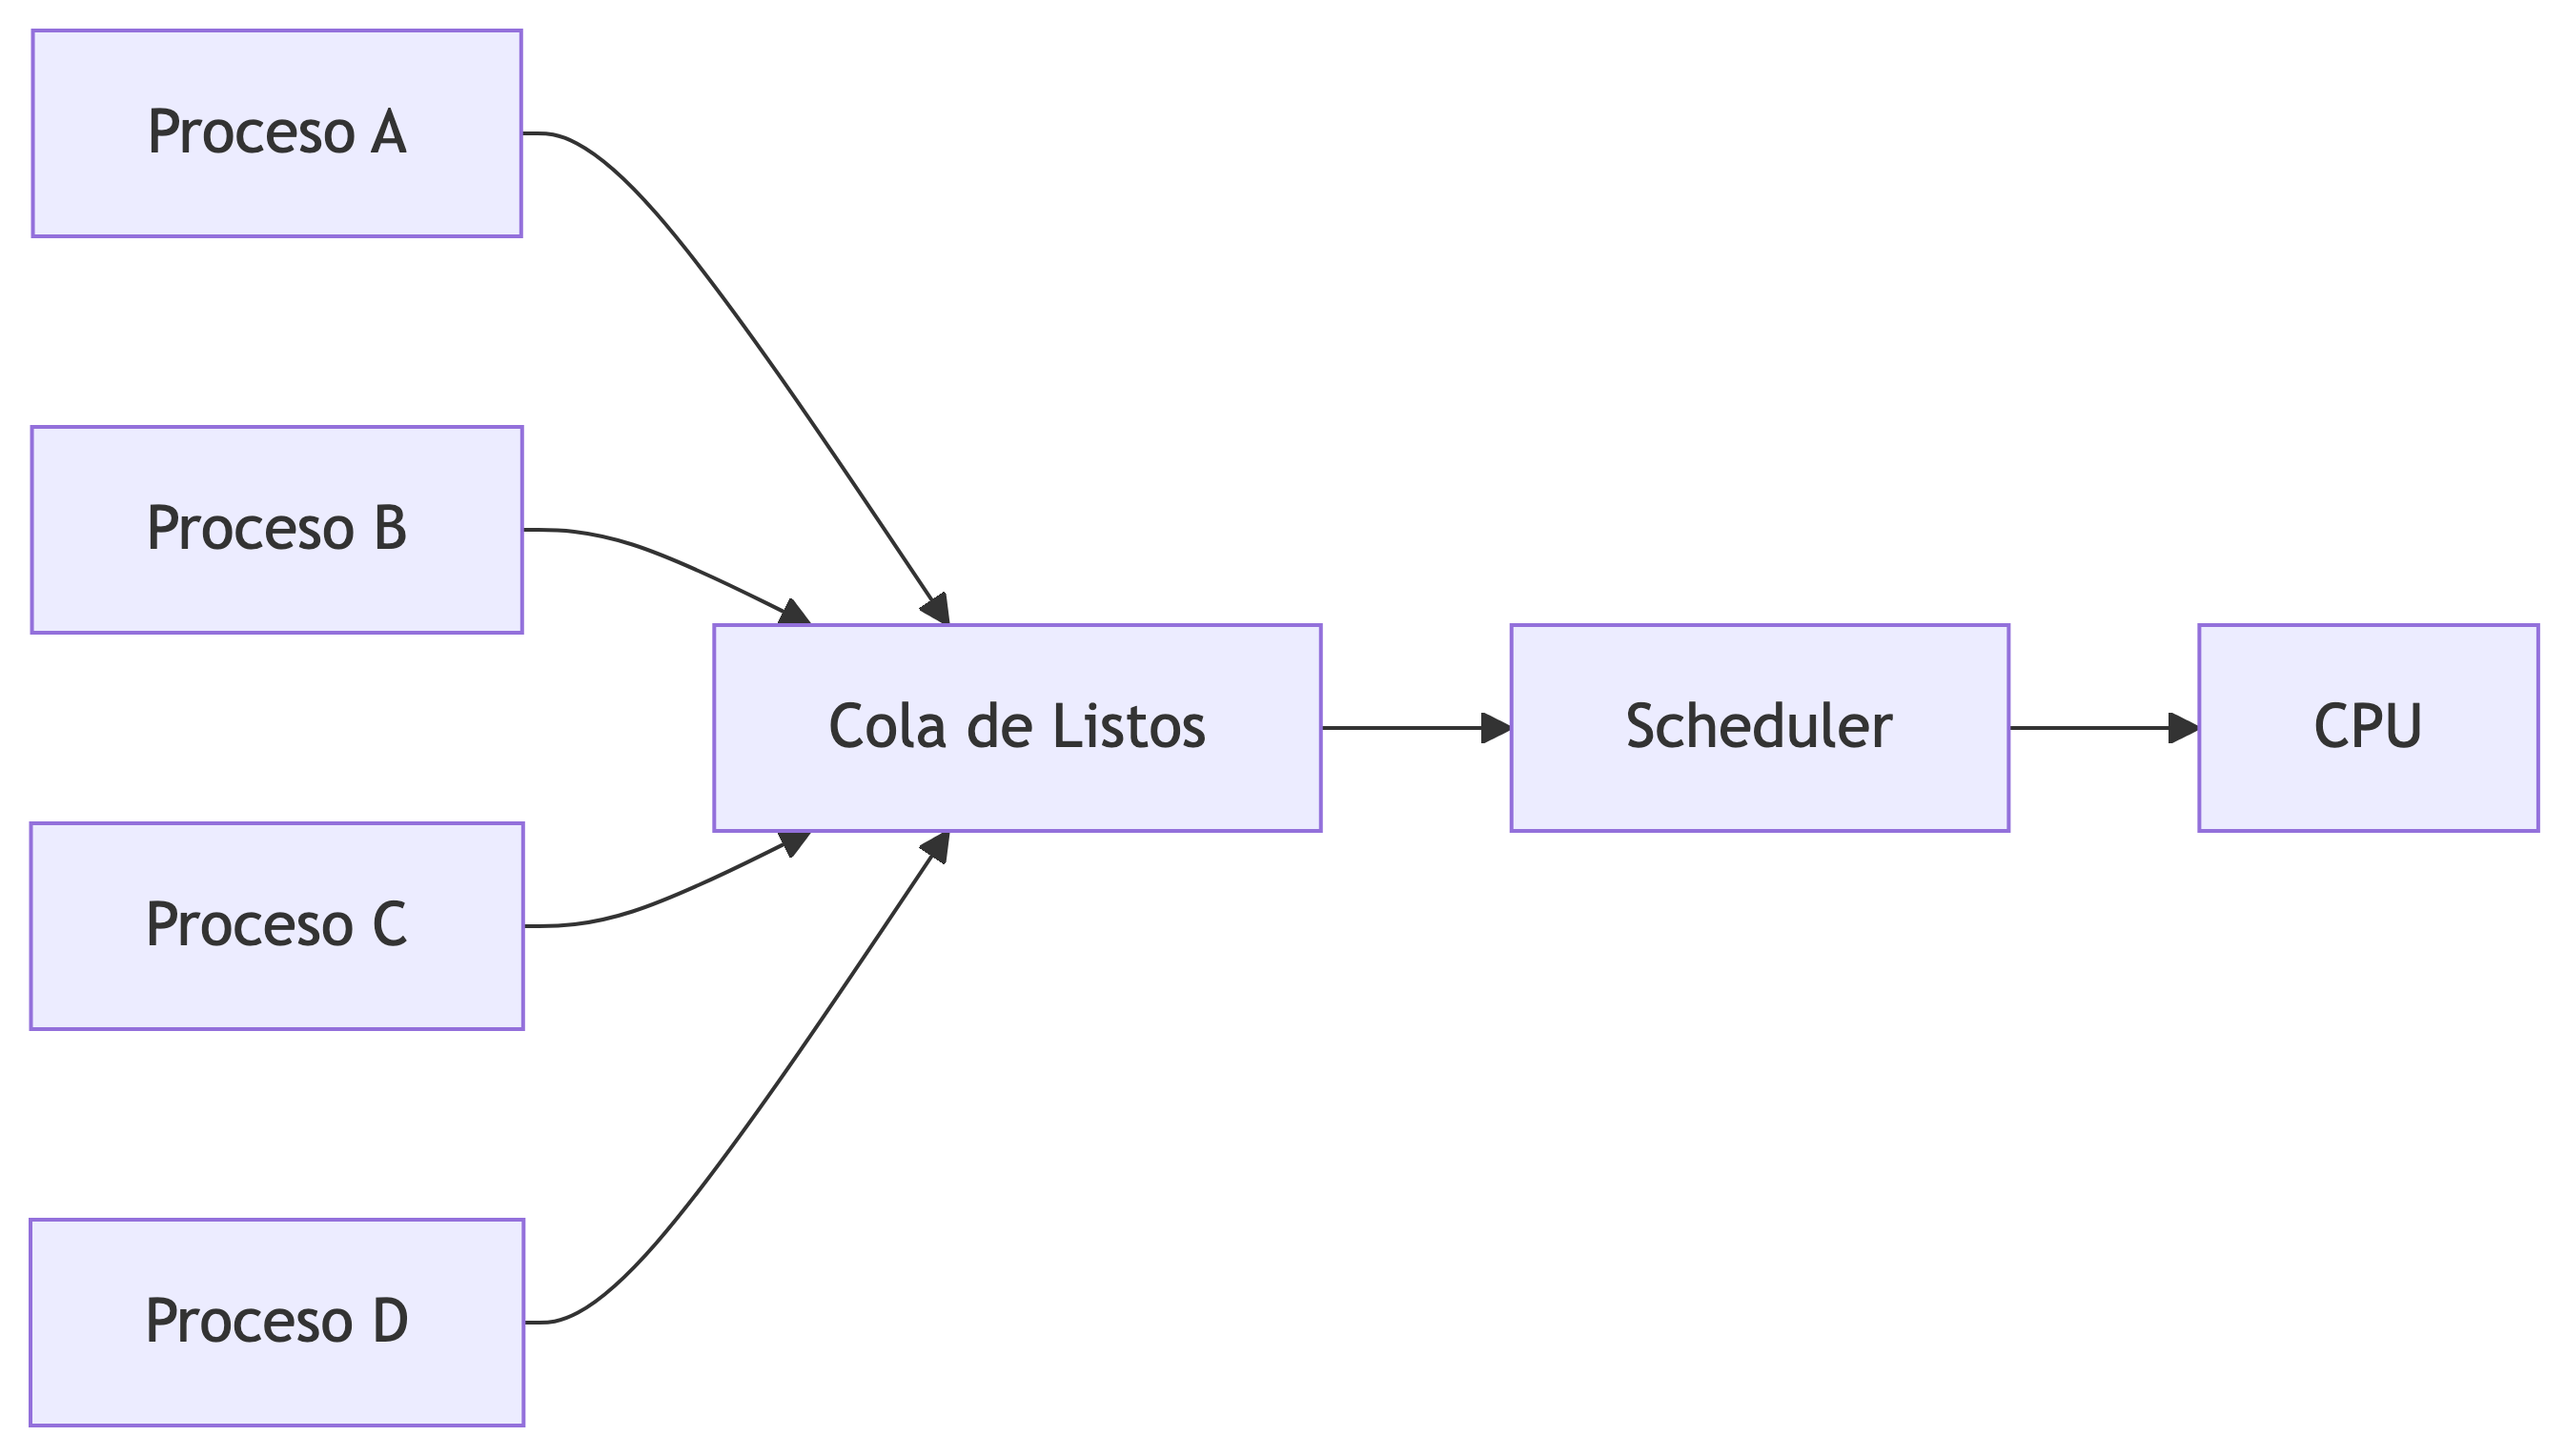
\includegraphics[width=7.02in,height=3.98in]{capitulos/06_algoritmos_de_planificacion_files/figure-latex/mermaid-figure-1.png}

\begin{tcolorbox}[enhanced jigsaw, arc=.35mm, bottomrule=.15mm, bottomtitle=1mm, breakable, colback=white, colbacktitle=quarto-callout-note-color!10!white, colframe=quarto-callout-note-color-frame, coltitle=black, left=2mm, leftrule=.75mm, opacityback=0, opacitybacktitle=0.6, rightrule=.15mm, title=\textcolor{quarto-callout-note-color}{\faInfo}\hspace{0.5em}{Idea clave}, titlerule=0mm, toprule=.15mm, toptitle=1mm]

La planificación busca utilizar el procesador de la forma más eficiente
posible.

\end{tcolorbox}

\bookmarksetup{startatroot}

\chapter{¿Qué aprenderemos en este
capítulo?}\label{quuxe9-aprenderemos-en-este-capuxedtulo}

Estudiaremos:

\begin{enumerate}
\def\labelenumi{\arabic{enumi}.}
\tightlist
\item
  FCFS (FIFO)
\item
  SJF
\item
  Prioridades
\item
  Round Robin
\end{enumerate}

Y al finalizar compararemos cuándo conviene utilizar cada uno.

\bookmarksetup{startatroot}

\chapter{Preparándonos para la siguiente
sección}\label{preparuxe1ndonos-para-la-siguiente-secciuxf3n}

Ahora estudiaremos al componente encargado de tomar estas decisiones:
\textbf{el Scheduler}, trabajando en conjunto con el Kernel.

\bookmarksetup{startatroot}

\chapter{El Scheduler, el Dispatcher y el
Kernel}\label{el-scheduler-el-dispatcher-y-el-kernel}

Hasta este momento sabemos que existen varios procesos esperando
utilizar el procesador.

La siguiente pregunta es:

\begin{quote}
\textbf{¿Quién toma la decisión de cuál proceso debe ejecutarse?}
\end{quote}

La respuesta involucra tres componentes importantes del Sistema
Operativo.

\bookmarksetup{startatroot}

\chapter{El Scheduler}\label{el-scheduler}

El \textbf{Scheduler} (Planificador) es el encargado de seleccionar el
siguiente proceso que utilizará el CPU.

Para tomar esta decisión analiza información almacenada en el PCB de
cada proceso.

Entre los principales criterios se encuentran:

\begin{itemize}
\tightlist
\item
  Tiempo de llegada.
\item
  Tiempo estimado de ejecución.
\item
  Prioridad.
\item
  Estado del proceso.
\item
  Algoritmo de planificación utilizado.
\end{itemize}

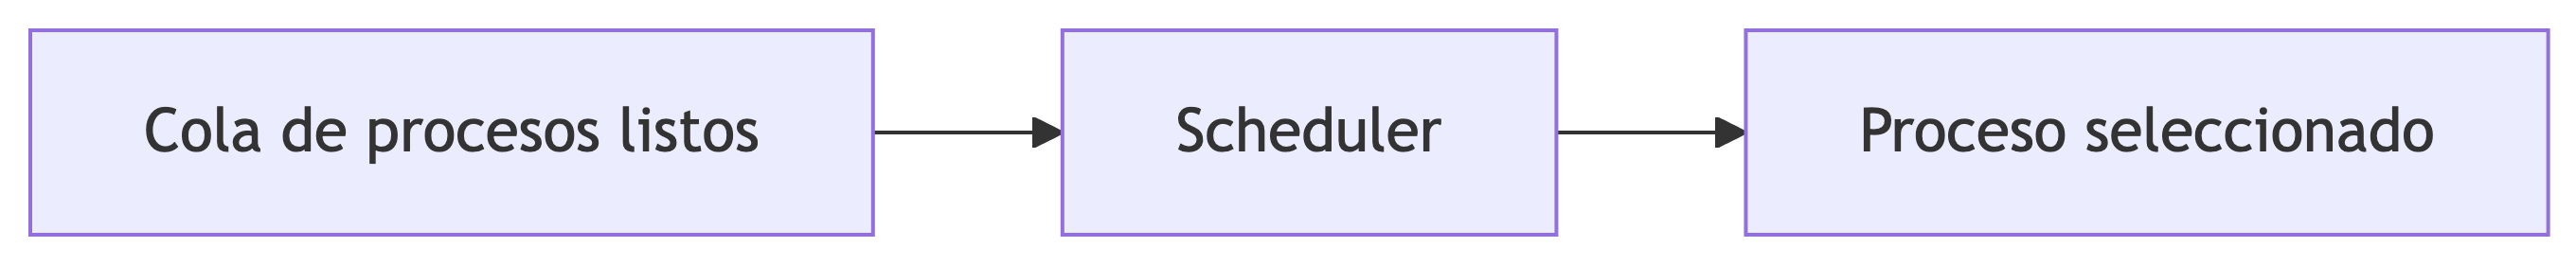
\includegraphics[width=7.09in,height=0.73in]{capitulos/06_algoritmos_de_planificacion_files/figure-latex/mermaid-figure-11.png}

\begin{tcolorbox}[enhanced jigsaw, arc=.35mm, bottomrule=.15mm, bottomtitle=1mm, breakable, colback=white, colbacktitle=quarto-callout-note-color!10!white, colframe=quarto-callout-note-color-frame, coltitle=black, left=2mm, leftrule=.75mm, opacityback=0, opacitybacktitle=0.6, rightrule=.15mm, title=\textcolor{quarto-callout-note-color}{\faInfo}\hspace{0.5em}{Idea importante}, titlerule=0mm, toprule=.15mm, toptitle=1mm]

El Scheduler \textbf{decide}, pero todavía no entrega el procesador al
proceso.

\end{tcolorbox}

\begin{center}\rule{0.5\linewidth}{0.5pt}\end{center}

\bookmarksetup{startatroot}

\chapter{El Dispatcher}\label{el-dispatcher}

Una vez que el Scheduler selecciona el proceso, entra en acción el
\textbf{Dispatcher}.

Su trabajo consiste en:

\begin{itemize}
\tightlist
\item
  Guardar el contexto del proceso que abandona el CPU.
\item
  Restaurar el contexto del proceso seleccionado.
\item
  Entregar el control del procesador.
\end{itemize}

Este procedimiento recibe el nombre de \textbf{Cambio de Contexto
(Context Switch)}.

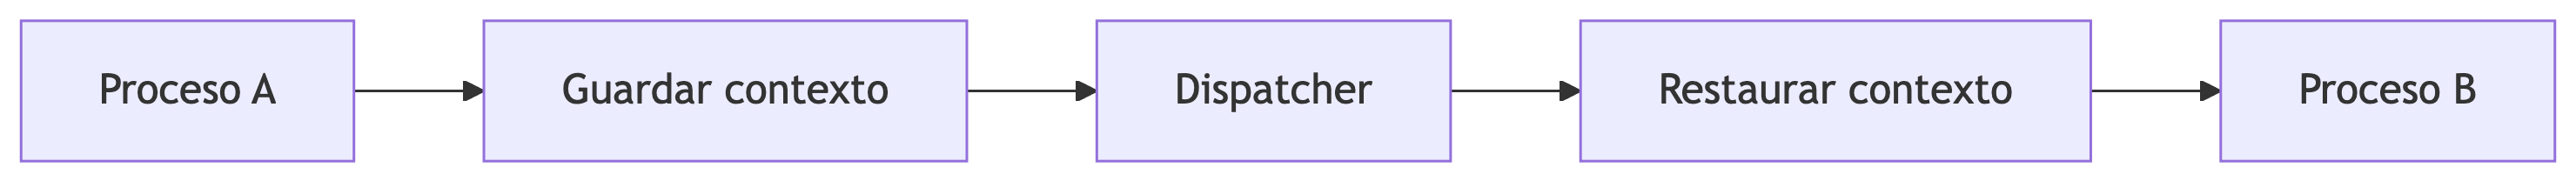
\includegraphics[width=10.32in,height=0.73in]{capitulos/06_algoritmos_de_planificacion_files/figure-latex/mermaid-figure-10.png}

\begin{center}\rule{0.5\linewidth}{0.5pt}\end{center}

\bookmarksetup{startatroot}

\chapter{¿Qué hace realmente el
Kernel?}\label{quuxe9-hace-realmente-el-kernel}

El Kernel coordina todo este proceso.

Mientras el Scheduler decide y el Dispatcher ejecuta el cambio, el
Kernel:

\begin{itemize}
\tightlist
\item
  Mantiene la cola de procesos listos.
\item
  Administra los PCB.
\item
  Controla las interrupciones.
\item
  Coordina el cambio de contexto.
\item
  Garantiza que un solo proceso utilice el CPU al mismo tiempo.
\end{itemize}

\begin{tcolorbox}[enhanced jigsaw, arc=.35mm, bottomrule=.15mm, bottomtitle=1mm, breakable, colback=white, colbacktitle=quarto-callout-tip-color!10!white, colframe=quarto-callout-tip-color-frame, coltitle=black, left=2mm, leftrule=.75mm, opacityback=0, opacitybacktitle=0.6, rightrule=.15mm, title=\textcolor{quarto-callout-tip-color}{\faLightbulb}\hspace{0.5em}{Recuerda}, titlerule=0mm, toprule=.15mm, toptitle=1mm]

\textbf{Scheduler} → Decide.

\textbf{Dispatcher} → Ejecuta el cambio.

\textbf{Kernel} → Coordina todo el proceso.

\end{tcolorbox}

\bookmarksetup{startatroot}

\chapter{¿Cómo trabajan juntos?}\label{cuxf3mo-trabajan-juntos}

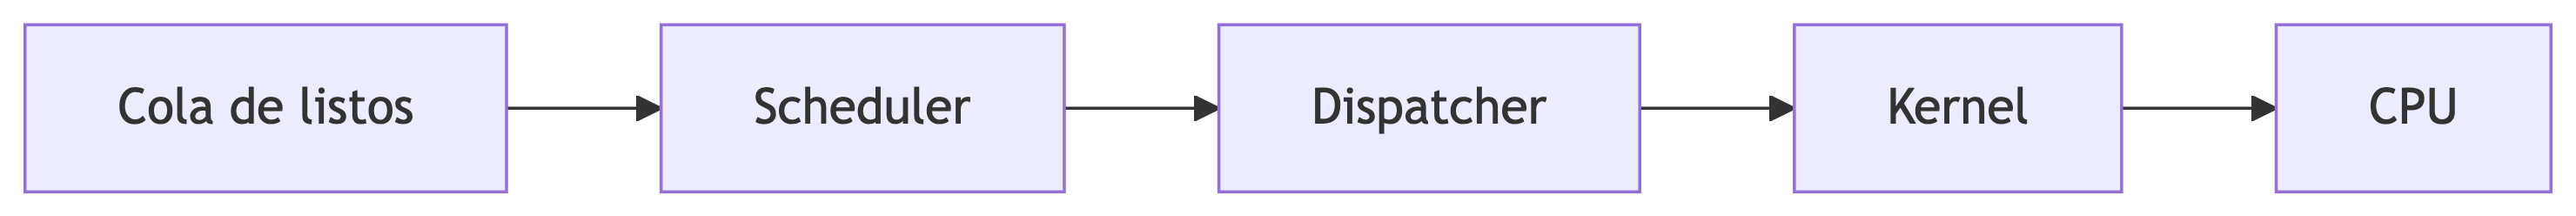
\includegraphics[width=8.68in,height=0.73in]{capitulos/06_algoritmos_de_planificacion_files/figure-latex/mermaid-figure-9.png}

\bookmarksetup{startatroot}

\chapter{Preparándonos para el primer
algoritmo}\label{preparuxe1ndonos-para-el-primer-algoritmo}

Ahora que comprendemos quién toma las decisiones, comenzaremos con el
algoritmo más sencillo de todos:

\textbf{FCFS (First Come, First Served)}, también conocido como
\textbf{FIFO (First In, First Out)}.

\bookmarksetup{startatroot}

\chapter{Algoritmo FCFS (FIFO)}\label{algoritmo-fcfs-fifo}

Ahora estudiaremos el algoritmo de planificación más sencillo.

Su nombre proviene de \textbf{First Come, First Served}, que significa:

\begin{quote}
\textbf{El primero en llegar, es el primero en ser atendido.}
\end{quote}

También se conoce como \textbf{FIFO (First In, First Out)}.

\bookmarksetup{startatroot}

\chapter{Un ejemplo cotidiano}\label{un-ejemplo-cotidiano}

Imagina una fila en la cafetería de la universidad.

Los estudiantes llegan en este orden:

\begin{enumerate}
\def\labelenumi{\arabic{enumi}.}
\tightlist
\item
  Ana
\item
  Luis
\item
  Carlos
\item
  María
\end{enumerate}

La regla es muy simple:

\begin{itemize}
\tightlist
\item
  Nadie puede adelantar a otro.
\item
  El primero en llegar será el primero en ser atendido.
\end{itemize}

FCFS funciona exactamente igual.

\bookmarksetup{startatroot}

\chapter{¿Cómo trabaja FCFS?}\label{cuxf3mo-trabaja-fcfs}

Cada proceso se coloca al final de la cola de listos.

Cuando el CPU queda libre, el Scheduler selecciona el proceso que lleva
más tiempo esperando.

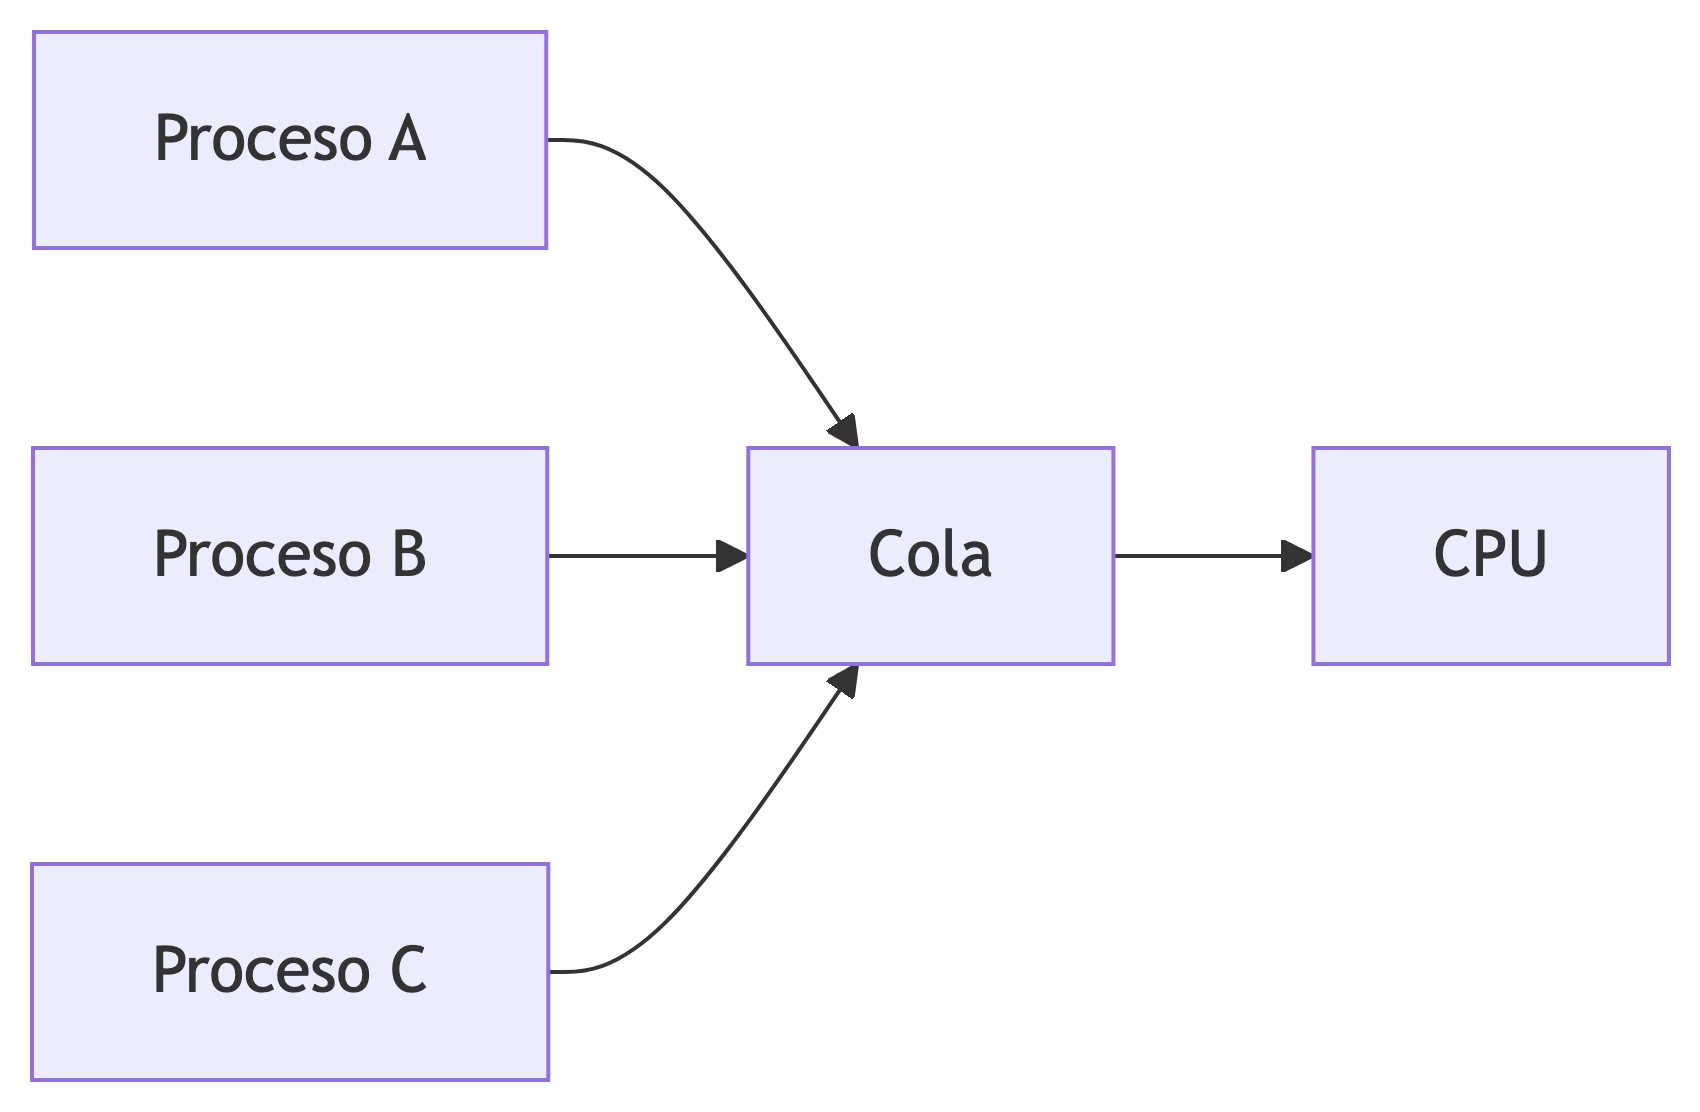
\includegraphics[width=4.43in,height=2.9in]{capitulos/06_algoritmos_de_planificacion_files/figure-latex/mermaid-figure-8.png}

\begin{tcolorbox}[enhanced jigsaw, arc=.35mm, bottomrule=.15mm, bottomtitle=1mm, breakable, colback=white, colbacktitle=quarto-callout-note-color!10!white, colframe=quarto-callout-note-color-frame, coltitle=black, left=2mm, leftrule=.75mm, opacityback=0, opacitybacktitle=0.6, rightrule=.15mm, title=\textcolor{quarto-callout-note-color}{\faInfo}\hspace{0.5em}{Idea importante}, titlerule=0mm, toprule=.15mm, toptitle=1mm]

Una vez que un proceso obtiene el CPU, \textbf{no será interrumpido}
hasta finalizar su ejecución.

\end{tcolorbox}

\bookmarksetup{startatroot}

\chapter{Ejemplo}\label{ejemplo-1}

Utilizaremos los mismos procesos mostrados en la presentación de clase.
fileciteturn13file0L5-L8

{\def\LTcaptype{none} % do not increment counter
\begin{longtable}[]{@{}lrr@{}}
\toprule\noalign{}
Proceso & Llegada & CPU \\
\midrule\noalign{}
\endhead
\bottomrule\noalign{}
\endlastfoot
A & 0 & 3 \\
B & 1 & 2 \\
C & 3 & 4 \\
D & 4 & 2 \\
E & 7 & 5 \\
F & 9 & 3 \\
\end{longtable}
}

\bookmarksetup{startatroot}

\chapter{Diagrama de Gantt}\label{diagrama-de-gantt}

\begin{Shaded}
\begin{Highlighting}[]
\NormalTok{0      3    5        9   11        16   19}
\NormalTok{|{-}{-}{-}A{-}{-}{-}|{-}{-}B{-}{-}|{-}{-}{-}{-}C{-}{-}{-}{-}|{-}D{-}|{-}{-}{-}{-}{-}E{-}{-}{-}{-}{-}|{-}F{-}|}
\end{Highlighting}
\end{Shaded}

Observa que el orden depende únicamente del momento en que cada proceso
llegó al sistema.

\bookmarksetup{startatroot}

\chapter{Ventajas}\label{ventajas-3}

\begin{itemize}
\tightlist
\item
  Fácil de implementar.
\item
  Poco costo de administración.
\item
  Ideal para sistemas sencillos.
\end{itemize}

\bookmarksetup{startatroot}

\chapter{Desventajas}\label{desventajas}

\begin{itemize}
\tightlist
\item
  Un proceso muy largo puede retrasar a todos los demás.
\item
  Los procesos cortos pueden esperar demasiado.
\item
  No es adecuado para sistemas interactivos.
\end{itemize}

\bookmarksetup{startatroot}

\chapter{¿Cuándo utilizar FCFS?}\label{cuuxe1ndo-utilizar-fcfs}

Es recomendable cuando:

\begin{itemize}
\tightlist
\item
  Todos los procesos tienen duraciones similares.
\item
  La simplicidad es más importante que el rendimiento.
\item
  Se trata de sistemas pequeños.
\end{itemize}

\begin{tcolorbox}[enhanced jigsaw, arc=.35mm, bottomrule=.15mm, bottomtitle=1mm, breakable, colback=white, colbacktitle=quarto-callout-tip-color!10!white, colframe=quarto-callout-tip-color-frame, coltitle=black, left=2mm, leftrule=.75mm, opacityback=0, opacitybacktitle=0.6, rightrule=.15mm, title=\textcolor{quarto-callout-tip-color}{\faLightbulb}\hspace{0.5em}{Reflexiona}, titlerule=0mm, toprule=.15mm, toptitle=1mm]

¿Qué ocurriría si el primer proceso necesitara 30 segundos de CPU y los
demás solo 2 segundos?

¿Sería justo utilizar FCFS?

\end{tcolorbox}

\bookmarksetup{startatroot}

\chapter{Preparándonos para el siguiente
algoritmo}\label{preparuxe1ndonos-para-el-siguiente-algoritmo}

FCFS considera únicamente el orden de llegada.

¿Y si el Sistema Operativo eligiera primero el proceso más corto?

Eso responderá el algoritmo \textbf{SJF (Shortest Job First)}.

\bookmarksetup{startatroot}

\chapter{Algoritmo SJF (Shortest Job
First)}\label{algoritmo-sjf-shortest-job-first}

Después de conocer FCFS surge una pregunta interesante.

\begin{quote}
¿Y si en lugar de atender al primero que llegó, atendiéramos primero al
proceso que terminará más rápido?
\end{quote}

Esa es precisamente la idea del algoritmo \textbf{SJF (Shortest Job
First)}.

\bookmarksetup{startatroot}

\chapter{Un ejemplo cotidiano}\label{un-ejemplo-cotidiano-1}

Imagina una fotocopiadora en la universidad.

Hay cuatro estudiantes esperando:

{\def\LTcaptype{none} % do not increment counter
\begin{longtable}[]{@{}lr@{}}
\toprule\noalign{}
Estudiante & Hojas \\
\midrule\noalign{}
\endhead
\bottomrule\noalign{}
\endlastfoot
Ana & 2 \\
Luis & 25 \\
Carlos & 4 \\
María & 1 \\
\end{longtable}
}

Si queremos atender al mayor número de personas en el menor tiempo
posible, comenzaríamos por los trabajos más cortos.

SJF aplica exactamente esa estrategia.

\bookmarksetup{startatroot}

\chapter{¿Cómo trabaja SJF?}\label{cuxf3mo-trabaja-sjf}

Cuando el procesador queda libre, el Scheduler selecciona el proceso con
el \textbf{menor tiempo estimado de CPU} entre los que están listos.

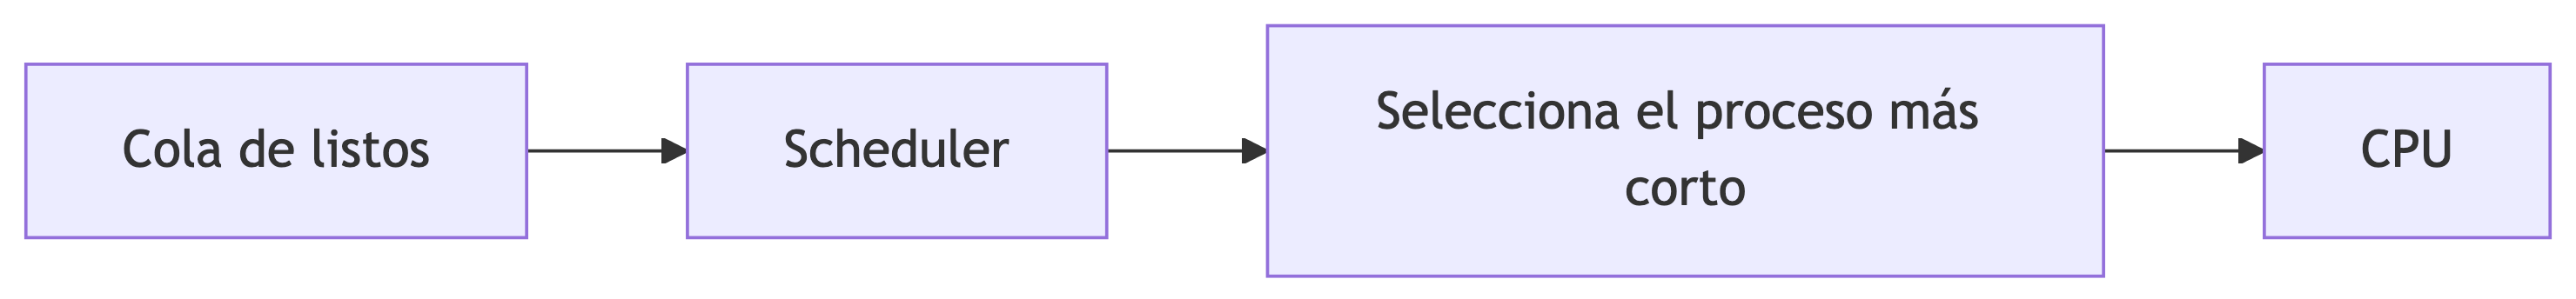
\includegraphics[width=8.34in,height=0.98in]{capitulos/06_algoritmos_de_planificacion_files/figure-latex/mermaid-figure-7.png}

\begin{tcolorbox}[enhanced jigsaw, arc=.35mm, bottomrule=.15mm, bottomtitle=1mm, breakable, colback=white, colbacktitle=quarto-callout-note-color!10!white, colframe=quarto-callout-note-color-frame, coltitle=black, left=2mm, leftrule=.75mm, opacityback=0, opacitybacktitle=0.6, rightrule=.15mm, title=\textcolor{quarto-callout-note-color}{\faInfo}\hspace{0.5em}{Idea importante}, titlerule=0mm, toprule=.15mm, toptitle=1mm]

SJF no observa únicamente el orden de llegada; también considera cuánto
tiempo tardará cada proceso en ejecutarse.

\end{tcolorbox}

\bookmarksetup{startatroot}

\chapter{Ejemplo}\label{ejemplo-2}

Utilizaremos los mismos procesos del ejercicio de clase.
fileciteturn13file0L7-L8

{\def\LTcaptype{none} % do not increment counter
\begin{longtable}[]{@{}lrr@{}}
\toprule\noalign{}
Proceso & Llegada & CPU \\
\midrule\noalign{}
\endhead
\bottomrule\noalign{}
\endlastfoot
A & 0 & 3 \\
B & 1 & 2 \\
C & 3 & 4 \\
D & 4 & 2 \\
E & 7 & 5 \\
F & 9 & 3 \\
\end{longtable}
}

Observa el diagrama de Gantt de la presentación y analiza cómo cambian
las decisiones del Scheduler al elegir el proceso más corto disponible.
fileciteturn13file0L7-L8

\bookmarksetup{startatroot}

\chapter{Ventajas}\label{ventajas-4}

\begin{itemize}
\tightlist
\item
  Reduce el tiempo promedio de espera.
\item
  Favorece procesos cortos.
\item
  Mejora el rendimiento en muchas cargas de trabajo.
\end{itemize}

\bookmarksetup{startatroot}

\chapter{Desventajas}\label{desventajas-1}

\begin{itemize}
\tightlist
\item
  Requiere estimar el tiempo de ejecución.
\item
  Los procesos largos pueden esperar demasiado (inanición).
\end{itemize}

\bookmarksetup{startatroot}

\chapter{¿Cuándo utilizar SJF?}\label{cuuxe1ndo-utilizar-sjf}

Es recomendable cuando:

\begin{itemize}
\tightlist
\item
  Se conoce o puede estimarse la duración de los procesos.
\item
  El objetivo es reducir el tiempo promedio de espera.
\end{itemize}

\begin{tcolorbox}[enhanced jigsaw, arc=.35mm, bottomrule=.15mm, bottomtitle=1mm, breakable, colback=white, colbacktitle=quarto-callout-warning-color!10!white, colframe=quarto-callout-warning-color-frame, coltitle=black, left=2mm, leftrule=.75mm, opacityback=0, opacitybacktitle=0.6, rightrule=.15mm, title=\textcolor{quarto-callout-warning-color}{\faExclamationTriangle}\hspace{0.5em}{Error común}, titlerule=0mm, toprule=.15mm, toptitle=1mm]

SJF no siempre ejecuta el proceso más corto del sistema.

Solo compara los procesos que \textbf{ya se encuentran en la cola de
listos}.

\end{tcolorbox}

\bookmarksetup{startatroot}

\chapter{FCFS vs.~SJF}\label{fcfs-vs.-sjf}

{\def\LTcaptype{none} % do not increment counter
\begin{longtable}[]{@{}lll@{}}
\toprule\noalign{}
Característica & FCFS & SJF \\
\midrule\noalign{}
\endhead
\bottomrule\noalign{}
\endlastfoot
Criterio & Orden de llegada & Menor tiempo de CPU \\
Fácil de implementar & ✔ & ✘ \\
Reduce espera promedio & ✘ & ✔ \\
Riesgo de espera excesiva (Inanición / Starvation) & Bajo & Alto \\
\end{longtable}
}

\begin{tcolorbox}[enhanced jigsaw, arc=.35mm, bottomrule=.15mm, bottomtitle=1mm, breakable, colback=white, colbacktitle=quarto-callout-note-color!10!white, colframe=quarto-callout-note-color-frame, coltitle=black, left=2mm, leftrule=.75mm, opacityback=0, opacitybacktitle=0.6, rightrule=.15mm, title=\textcolor{quarto-callout-note-color}{\faInfo}\hspace{0.5em}{¿Qué significa el riesgo de inanición (Starvation)?}, titlerule=0mm, toprule=.15mm, toptitle=1mm]

En Sistemas Operativos, la \textbf{inanición} (\emph{Starvation}) ocurre
cuando un proceso espera tanto tiempo por el procesador que, en la
práctica, casi nunca llega a ejecutarse.

Esto sucede porque otros procesos son seleccionados continuamente antes
que él.

\subsection{Ejemplo}\label{ejemplo-3}

Supongamos que tenemos los siguientes procesos:

{\def\LTcaptype{none} % do not increment counter
\begin{longtable}[]{@{}cr@{}}
\toprule\noalign{}
Proceso & Tiempo de CPU \\
\midrule\noalign{}
\endhead
\bottomrule\noalign{}
\endlastfoot
A & 20 s \\
B & 2 s \\
C & 1 s \\
D & 3 s \\
E & 2 s \\
\end{longtable}
}

Si el Sistema Operativo utiliza \textbf{SJF (Shortest Job First)},
siempre elegirá primero los procesos con menor tiempo de ejecución.

Si mientras el proceso \textbf{A} espera siguen llegando procesos más
pequeños, estos continuarán siendo seleccionados antes que él.

Como consecuencia, el proceso \textbf{A} podría permanecer esperando
durante mucho tiempo.

Por esta razón decimos que \textbf{SJF presenta un mayor riesgo de
inanición (Starvation)} para los procesos largos.

En cambio, con \textbf{FCFS}, todos los procesos conservan su turno de
llegada, por lo que, tarde o temprano, todos serán ejecutados.

\end{tcolorbox}

\bookmarksetup{startatroot}

\chapter{Preparándonos para el siguiente
algoritmo}\label{preparuxe1ndonos-para-el-siguiente-algoritmo-1}

Hasta ahora hemos considerado el orden de llegada y la duración del
proceso.

¿Y si algunos procesos fueran más importantes que otros?

Eso nos llevará al algoritmo de \textbf{Prioridades}.

\bookmarksetup{startatroot}

\chapter{Algoritmo de Planificación por
Prioridades}\label{algoritmo-de-planificaciuxf3n-por-prioridades}

Hasta ahora hemos estudiado dos formas de seleccionar el siguiente
proceso:

\begin{itemize}
\tightlist
\item
  \textbf{FCFS:} el primero que llegó.
\item
  \textbf{SJF:} el proceso más corto.
\end{itemize}

Ahora analizaremos una tercera estrategia.

\begin{quote}
\textbf{¿Y si algunos procesos fueran más importantes que otros?}
\end{quote}

Ese es precisamente el objetivo del algoritmo de \textbf{Prioridades}.

\bookmarksetup{startatroot}

\chapter{Un ejemplo cotidiano}\label{un-ejemplo-cotidiano-2}

Imagina la sala de emergencias de un hospital.

Llegan cuatro pacientes casi al mismo tiempo.

\begin{itemize}
\tightlist
\item
  Un paciente con un resfriado.
\item
  Una persona con un brazo fracturado.
\item
  Un paciente con un paro cardíaco.
\item
  Una persona con una cortadura leve.
\end{itemize}

Aunque algunos hayan llegado antes, el médico atenderá primero al
paciente cuya condición sea más crítica.

El Sistema Operativo hace algo similar cuando utiliza prioridades.

\bookmarksetup{startatroot}

\chapter{¿Cómo trabaja?}\label{cuxf3mo-trabaja}

Cada proceso recibe un \textbf{nivel de prioridad}.

Cuando el CPU queda disponible, el Scheduler selecciona el proceso con
la prioridad más alta.

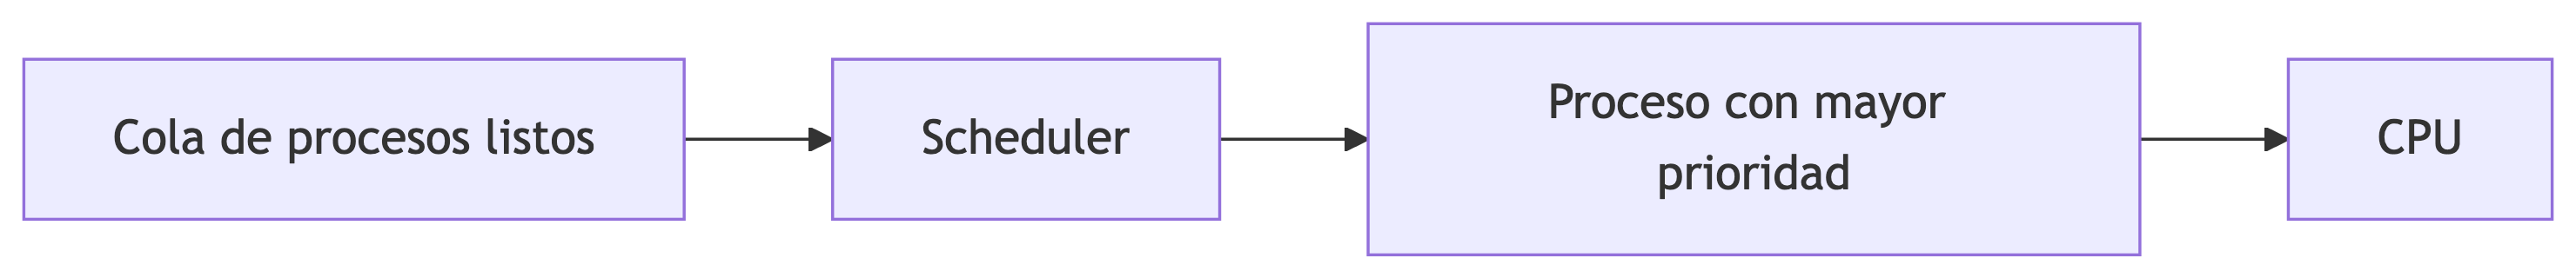
\includegraphics[width=9.04in,height=0.98in]{capitulos/06_algoritmos_de_planificacion_files/figure-latex/mermaid-figure-6.png}

\begin{tcolorbox}[enhanced jigsaw, arc=.35mm, bottomrule=.15mm, bottomtitle=1mm, breakable, colback=white, colbacktitle=quarto-callout-note-color!10!white, colframe=quarto-callout-note-color-frame, coltitle=black, left=2mm, leftrule=.75mm, opacityback=0, opacitybacktitle=0.6, rightrule=.15mm, title=\textcolor{quarto-callout-note-color}{\faInfo}\hspace{0.5em}{Idea importante}, titlerule=0mm, toprule=.15mm, toptitle=1mm]

En este algoritmo, \textbf{la prioridad es más importante que el orden
de llegada}.

\end{tcolorbox}

\bookmarksetup{startatroot}

\chapter{Ejemplo}\label{ejemplo-4}

Supongamos los siguientes procesos.

{\def\LTcaptype{none} % do not increment counter
\begin{longtable}[]{@{}cr@{}}
\toprule\noalign{}
Proceso & Prioridad \\
\midrule\noalign{}
\endhead
\bottomrule\noalign{}
\endlastfoot
A & 3 \\
B & 1 \\
C & 4 \\
D & 2 \\
\end{longtable}
}

\begin{quote}
En este ejemplo, \textbf{1 representa la prioridad más alta}.
\end{quote}

El orden de ejecución será:

\begin{Shaded}
\begin{Highlighting}[]
\NormalTok{B → D → A → C}
\end{Highlighting}
\end{Shaded}

\bookmarksetup{startatroot}

\chapter{Diagrama de Gantt}\label{diagrama-de-gantt-1}

\begin{Shaded}
\begin{Highlighting}[]
\NormalTok{0      2      5      8      10}
\NormalTok{|{-}{-}B{-}{-}|{-}{-}{-}D{-}{-}{-}|{-}{-}{-}A{-}{-}{-}|{-}{-}C{-}{-}|}
\end{Highlighting}
\end{Shaded}

\subsection{¿Quién asigna la
prioridad?}\label{quiuxe9n-asigna-la-prioridad}

La prioridad no se asigna al azar.

Generalmente es determinada por el Sistema Operativo considerando
aspectos como:

\begin{itemize}
\tightlist
\item
  La importancia del proceso.
\item
  El tipo de aplicación.
\item
  El usuario que ejecuta el programa.
\item
  El tiempo que lleva esperando.
\item
  Las políticas definidas por el Sistema Operativo.
\end{itemize}

En muchos Sistemas Operativos modernos, la prioridad puede cambiar
durante la ejecución para mejorar el rendimiento y evitar que algunos
procesos esperen demasiado tiempo.

\bookmarksetup{startatroot}

\chapter{Ventajas}\label{ventajas-5}

\begin{itemize}
\tightlist
\item
  Permite atender primero los procesos más importantes.
\item
  Muy utilizado en sistemas operativos modernos.
\item
  Adecuado para sistemas de tiempo real.
\end{itemize}

\bookmarksetup{startatroot}

\chapter{Desventajas}\label{desventajas-2}

\begin{itemize}
\tightlist
\item
  Los procesos de baja prioridad pueden esperar demasiado tiempo.
\item
  También puede presentarse \textbf{inanición (Starvation)} si
  continuamente llegan procesos con mayor prioridad.
\end{itemize}

\begin{tcolorbox}[enhanced jigsaw, arc=.35mm, bottomrule=.15mm, bottomtitle=1mm, breakable, colback=white, colbacktitle=quarto-callout-warning-color!10!white, colframe=quarto-callout-warning-color-frame, coltitle=black, left=2mm, leftrule=.75mm, opacityback=0, opacitybacktitle=0.6, rightrule=.15mm, title=\textcolor{quarto-callout-warning-color}{\faExclamationTriangle}\hspace{0.5em}{Error común}, titlerule=0mm, toprule=.15mm, toptitle=1mm]

Muchos estudiantes creen que el proceso con mayor prioridad siempre es
el primero que llegó.

Eso es incorrecto.

El criterio principal es la \textbf{prioridad}, no el tiempo de llegada.

\end{tcolorbox}

\bookmarksetup{startatroot}

\chapter{¿Cómo evitar la
inanición?}\label{cuxf3mo-evitar-la-inaniciuxf3n}

Muchos Sistemas Operativos implementan una técnica llamada \textbf{Aging
(Envejecimiento)}.

Consiste en aumentar gradualmente la prioridad de los procesos que
llevan mucho tiempo esperando.

De esta forma, tarde o temprano obtendrán acceso al procesador.

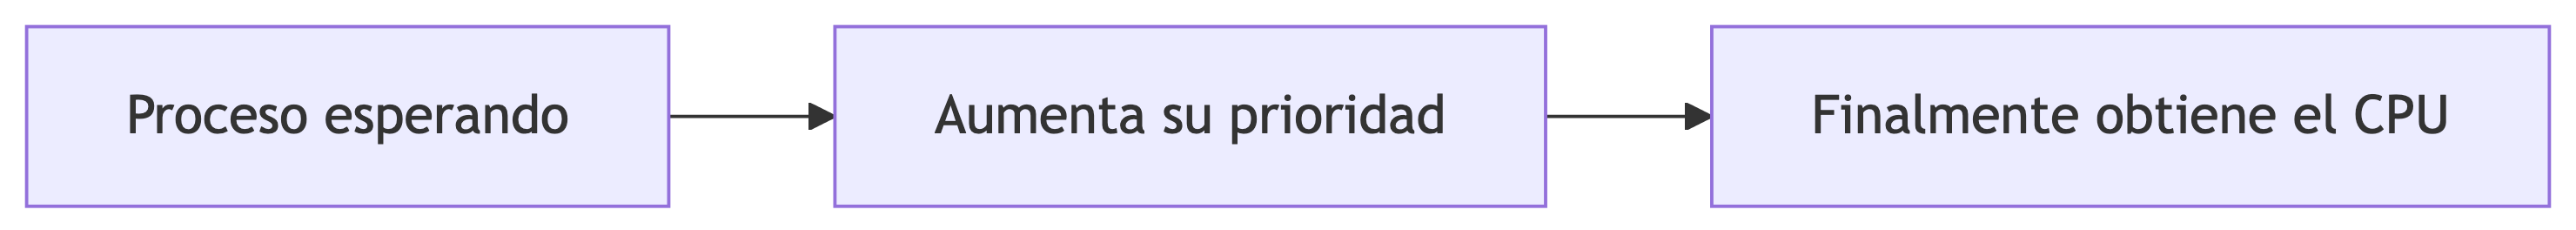
\includegraphics[width=8.07in,height=0.73in]{capitulos/06_algoritmos_de_planificacion_files/figure-latex/mermaid-figure-5.png}

\bookmarksetup{startatroot}

\chapter{Comparación}\label{comparaciuxf3n-1}

{\def\LTcaptype{none} % do not increment counter
\begin{longtable}[]{@{}
  >{\raggedright\arraybackslash}p{(\linewidth - 6\tabcolsep) * \real{0.2500}}
  >{\raggedright\arraybackslash}p{(\linewidth - 6\tabcolsep) * \real{0.2500}}
  >{\raggedright\arraybackslash}p{(\linewidth - 6\tabcolsep) * \real{0.2500}}
  >{\raggedright\arraybackslash}p{(\linewidth - 6\tabcolsep) * \real{0.2500}}@{}}
\toprule\noalign{}
\begin{minipage}[b]{\linewidth}\raggedright
Característica
\end{minipage} & \begin{minipage}[b]{\linewidth}\raggedright
FCFS
\end{minipage} & \begin{minipage}[b]{\linewidth}\raggedright
SJF
\end{minipage} & \begin{minipage}[b]{\linewidth}\raggedright
Prioridades
\end{minipage} \\
\midrule\noalign{}
\endhead
\bottomrule\noalign{}
\endlastfoot
Criterio principal & Orden de llegada & Menor tiempo de CPU & Mayor
prioridad \\
Fácil de implementar & ✔ & ✘ & ✔ \\
Riesgo de espera excesiva (Starvation) & Bajo & Alto & Alto \\
Uso recomendado & Sistemas sencillos & Optimizar tiempos & Sistemas
críticos \\
\end{longtable}
}

\begin{tcolorbox}[enhanced jigsaw, arc=.35mm, bottomrule=.15mm, bottomtitle=1mm, breakable, colback=white, colbacktitle=quarto-callout-tip-color!10!white, colframe=quarto-callout-tip-color-frame, coltitle=black, left=2mm, leftrule=.75mm, opacityback=0, opacitybacktitle=0.6, rightrule=.15mm, title=\textcolor{quarto-callout-tip-color}{\faLightbulb}\hspace{0.5em}{Reflexiona}, titlerule=0mm, toprule=.15mm, toptitle=1mm]

¿Por qué una alarma de incendio debería ejecutarse antes que un
reproductor de música?

¿Qué otros procesos de una computadora considerarías de alta prioridad?

\end{tcolorbox}

\bookmarksetup{startatroot}

\chapter{Preparándonos para el siguiente
algoritmo}\label{preparuxe1ndonos-para-el-siguiente-algoritmo-2}

Hasta ahora cada proceso conserva el CPU hasta finalizar.

En la siguiente sección estudiaremos \textbf{Round Robin}, donde todos
los procesos comparten el procesador por turnos mediante un
\textbf{Quantum}.

\bookmarksetup{startatroot}

\chapter{Algoritmo Round Robin (RR)}\label{algoritmo-round-robin-rr}

Hasta ahora hemos estudiado algoritmos donde un proceso conserva el
procesador hasta terminar su ejecución.

Pero surge un problema.

\begin{quote}
¿Qué ocurre si un proceso tarda varios minutos y los demás deben
esperar?
\end{quote}

Para resolver esta situación nació \textbf{Round Robin (RR)}.

\bookmarksetup{startatroot}

\chapter{Un ejemplo cotidiano}\label{un-ejemplo-cotidiano-3}

Imagina que un profesor debe atender dudas de diez estudiantes.

En lugar de dedicar todo el tiempo a un solo estudiante, decide
atenderlos por turnos.

Cada estudiante dispone de \textbf{2 minutos}.

Cuando el tiempo termina, pasa el siguiente estudiante.

Si aún tiene dudas, volverá a hacer fila.

Eso mismo hace Round Robin.

\bookmarksetup{startatroot}

\chapter{¿Qué es el Quantum?}\label{quuxe9-es-el-quantum}

El \textbf{Quantum} es el tiempo máximo que un proceso puede utilizar el
CPU antes de cederlo a otro proceso.

Si el proceso termina antes de consumir el Quantum, abandona el
procesador normalmente.

Si no termina, el Sistema Operativo lo envía nuevamente al final de la
cola de listos.

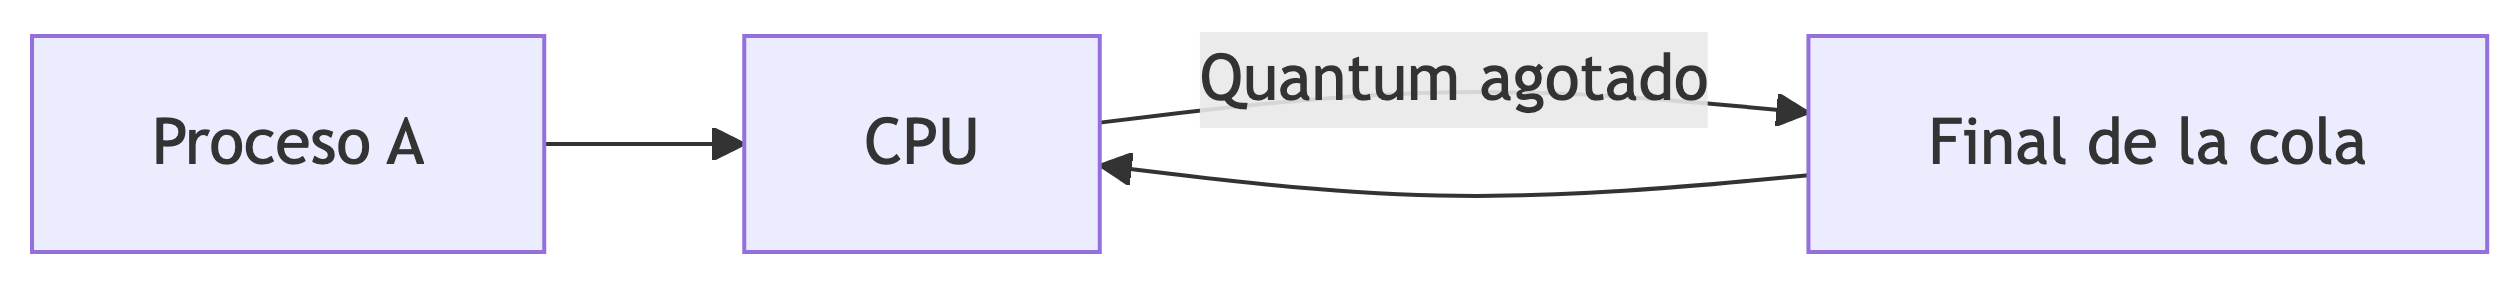
\includegraphics[width=6.56in,height=0.74in]{capitulos/06_algoritmos_de_planificacion_files/figure-latex/mermaid-figure-4.png}

\begin{tcolorbox}[enhanced jigsaw, arc=.35mm, bottomrule=.15mm, bottomtitle=1mm, breakable, colback=white, colbacktitle=quarto-callout-note-color!10!white, colframe=quarto-callout-note-color-frame, coltitle=black, left=2mm, leftrule=.75mm, opacityback=0, opacitybacktitle=0.6, rightrule=.15mm, title=\textcolor{quarto-callout-note-color}{\faInfo}\hspace{0.5em}{Idea clave}, titlerule=0mm, toprule=.15mm, toptitle=1mm]

Round Robin busca que \textbf{todos los procesos tengan oportunidad de
utilizar el procesador}, evitando esperas excesivas.

\end{tcolorbox}

\bookmarksetup{startatroot}

\chapter{Ejemplo}\label{ejemplo-5}

Supongamos un \textbf{Quantum = 2 ms}.

{\def\LTcaptype{none} % do not increment counter
\begin{longtable}[]{@{}cr@{}}
\toprule\noalign{}
Proceso & Tiempo de CPU \\
\midrule\noalign{}
\endhead
\bottomrule\noalign{}
\endlastfoot
A & 5 \\
B & 3 \\
C & 4 \\
\end{longtable}
}

\subsection{Primera ronda}\label{primera-ronda}

\begin{itemize}
\tightlist
\item
  A utiliza 2 ms (le quedan 3).
\item
  B utiliza 2 ms (le queda 1).
\item
  C utiliza 2 ms (le quedan 2).
\end{itemize}

\subsection{Segunda ronda}\label{segunda-ronda}

\begin{itemize}
\tightlist
\item
  A utiliza 2 ms (le queda 1).
\item
  B utiliza 1 ms y termina.
\item
  C utiliza 2 ms y termina.
\end{itemize}

\subsection{Tercera ronda}\label{tercera-ronda}

\begin{itemize}
\tightlist
\item
  A utiliza 1 ms y termina.
\end{itemize}

\bookmarksetup{startatroot}

\chapter{Diagrama de Gantt}\label{diagrama-de-gantt-2}

\begin{Shaded}
\begin{Highlighting}[]
\NormalTok{Quantum = 2 ms}

\NormalTok{0   2   4   6   8   9  11 12}
\NormalTok{| A | B | C | A | B | C | A |}
\end{Highlighting}
\end{Shaded}

\bookmarksetup{startatroot}

\chapter{Ventajas}\label{ventajas-6}

\begin{itemize}
\tightlist
\item
  Todos los procesos reciben tiempo de CPU.
\item
  Muy adecuado para sistemas interactivos.
\item
  Evita que un proceso monopolice el procesador.
\item
  Reduce la sensación de espera del usuario.
\end{itemize}

\bookmarksetup{startatroot}

\chapter{Desventajas}\label{desventajas-3}

\begin{itemize}
\tightlist
\item
  Requiere numerosos cambios de contexto.
\item
  Si el Quantum es demasiado pequeño, aumenta la sobrecarga.
\item
  Si el Quantum es demasiado grande, se parece a FCFS.
\end{itemize}

\section{¿Cómo elegir un buen
Quantum?}\label{cuxf3mo-elegir-un-buen-quantum}

\begin{itemize}
\tightlist
\item
  \textbf{Muy pequeño:} muchos cambios de contexto y menor rendimiento.
\item
  \textbf{Muy grande:} los procesos esperan demasiado.
\item
  \textbf{Adecuado:} equilibrio entre rendimiento y respuesta.
\end{itemize}

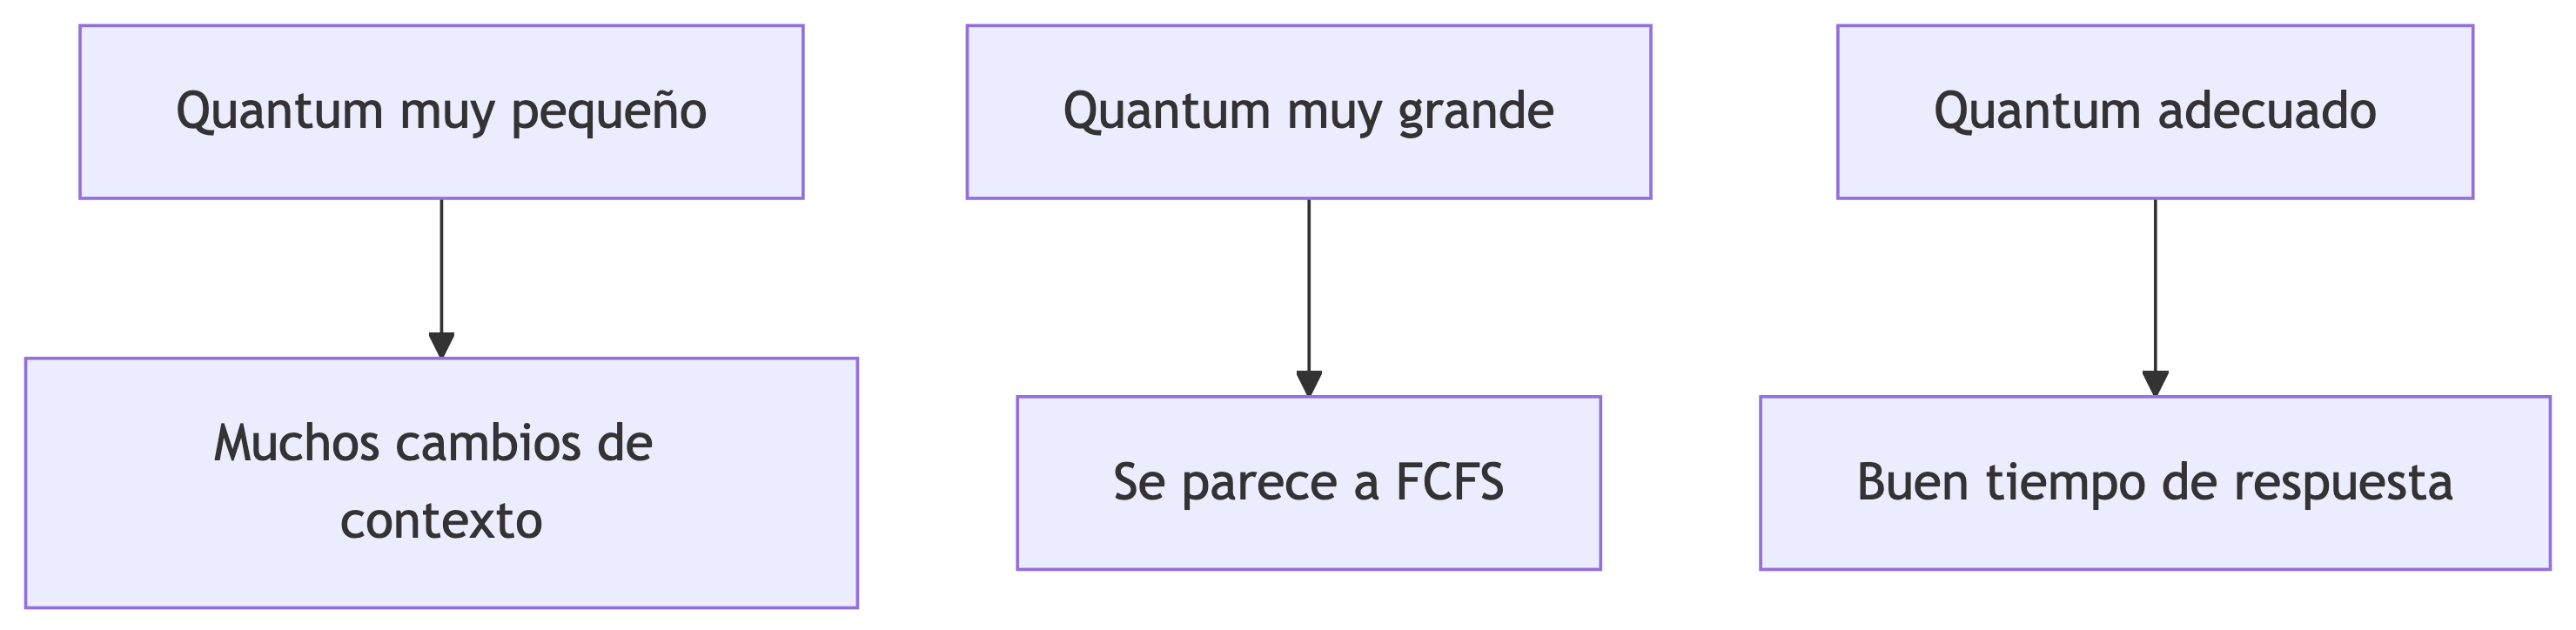
\includegraphics[width=8.39in,height=2.06in]{capitulos/06_algoritmos_de_planificacion_files/figure-latex/mermaid-figure-3.png}

\bookmarksetup{startatroot}

\chapter{Comparación general}\label{comparaciuxf3n-general-1}

{\def\LTcaptype{none} % do not increment counter
\begin{longtable}[]{@{}
  >{\raggedright\arraybackslash}p{(\linewidth - 6\tabcolsep) * \real{0.2500}}
  >{\raggedright\arraybackslash}p{(\linewidth - 6\tabcolsep) * \real{0.2500}}
  >{\raggedright\arraybackslash}p{(\linewidth - 6\tabcolsep) * \real{0.2500}}
  >{\raggedright\arraybackslash}p{(\linewidth - 6\tabcolsep) * \real{0.2500}}@{}}
\toprule\noalign{}
\begin{minipage}[b]{\linewidth}\raggedright
Algoritmo
\end{minipage} & \begin{minipage}[b]{\linewidth}\raggedright
Criterio
\end{minipage} & \begin{minipage}[b]{\linewidth}\raggedright
Principal ventaja
\end{minipage} & \begin{minipage}[b]{\linewidth}\raggedright
Principal desventaja
\end{minipage} \\
\midrule\noalign{}
\endhead
\bottomrule\noalign{}
\endlastfoot
FCFS & Orden de llegada & Muy simple & Esperas largas \\
SJF & Menor tiempo & Reduce espera promedio & Inanición \\
Prioridades & Mayor prioridad & Atiende procesos críticos & Inanición \\
Round Robin & Quantum & Equidad entre procesos & Más cambios de
contexto \\
\end{longtable}
}

\begin{tcolorbox}[enhanced jigsaw, arc=.35mm, bottomrule=.15mm, bottomtitle=1mm, breakable, colback=white, colbacktitle=quarto-callout-tip-color!10!white, colframe=quarto-callout-tip-color-frame, coltitle=black, left=2mm, leftrule=.75mm, opacityback=0, opacitybacktitle=0.6, rightrule=.15mm, title=\textcolor{quarto-callout-tip-color}{\faLightbulb}\hspace{0.5em}{Reflexiona}, titlerule=0mm, toprule=.15mm, toptitle=1mm]

¿Por qué Windows, Linux y Android utilizan algoritmos basados en Round
Robin para atender aplicaciones interactivas?

¿Qué ocurriría si un navegador web tuviera que esperar varios segundos
para volver a recibir tiempo de CPU?

\end{tcolorbox}

\bookmarksetup{startatroot}

\chapter{Preparándonos para el
cierre}\label{preparuxe1ndonos-para-el-cierre}

Ya conocemos los cuatro algoritmos clásicos de planificación.

En la siguiente sección los compararemos mediante un caso integrador y
resumiremos cuándo conviene utilizar cada uno.

\bookmarksetup{startatroot}

\chapter{Comparación general de los algoritmos de
planificación}\label{comparaciuxf3n-general-de-los-algoritmos-de-planificaciuxf3n}

Llegamos al final del capítulo.

Ahora ya conocemos los cuatro algoritmos clásicos de planificación del
CPU.

Antes de continuar con el siguiente tema, comparemos sus principales
características.

{\def\LTcaptype{none} % do not increment counter
\begin{longtable}[]{@{}
  >{\raggedright\arraybackslash}p{(\linewidth - 8\tabcolsep) * \real{0.2000}}
  >{\raggedright\arraybackslash}p{(\linewidth - 8\tabcolsep) * \real{0.2000}}
  >{\raggedright\arraybackslash}p{(\linewidth - 8\tabcolsep) * \real{0.2000}}
  >{\raggedright\arraybackslash}p{(\linewidth - 8\tabcolsep) * \real{0.2000}}
  >{\raggedright\arraybackslash}p{(\linewidth - 8\tabcolsep) * \real{0.2000}}@{}}
\toprule\noalign{}
\begin{minipage}[b]{\linewidth}\raggedright
Algoritmo
\end{minipage} & \begin{minipage}[b]{\linewidth}\raggedright
¿Cómo decide?
\end{minipage} & \begin{minipage}[b]{\linewidth}\raggedright
Ventaja principal
\end{minipage} & \begin{minipage}[b]{\linewidth}\raggedright
Desventaja principal
\end{minipage} & \begin{minipage}[b]{\linewidth}\raggedright
Uso recomendado
\end{minipage} \\
\midrule\noalign{}
\endhead
\bottomrule\noalign{}
\endlastfoot
\textbf{FCFS} & Primer proceso en llegar & Muy sencillo de implementar &
Puede generar largas esperas & Sistemas simples o por lotes \\
\textbf{SJF} & Menor tiempo de CPU & Reduce el tiempo promedio de espera
& Riesgo de inanición & Procesos con duración conocida \\
\textbf{Prioridades} & Mayor prioridad & Atiende primero procesos
críticos & Riesgo de inanición & Sistemas de tiempo real \\
\textbf{Round Robin} & Turnos mediante Quantum & Todos reciben tiempo de
CPU & Mayor cantidad de cambios de contexto & Sistemas interactivos \\
\end{longtable}
}

\begin{center}\rule{0.5\linewidth}{0.5pt}\end{center}

\bookmarksetup{startatroot}

\chapter{Caso integrador}\label{caso-integrador}

Supongamos que llegan simultáneamente los siguientes procesos:

{\def\LTcaptype{none} % do not increment counter
\begin{longtable}[]{@{}crr@{}}
\toprule\noalign{}
Proceso & CPU & Prioridad \\
\midrule\noalign{}
\endhead
\bottomrule\noalign{}
\endlastfoot
A & 8 & 3 \\
B & 2 & 1 \\
C & 4 & 4 \\
D & 3 & 2 \\
\end{longtable}
}

\section{Analiza}\label{analiza}

\begin{enumerate}
\def\labelenumi{\arabic{enumi}.}
\tightlist
\item
  ¿Qué proceso ejecutaría FCFS primero?
\item
  ¿Qué proceso elegiría SJF?
\item
  ¿Qué proceso seleccionaría Prioridades?
\item
  Si el Quantum = 2 ms, ¿cómo comenzaría Round Robin?
\end{enumerate}

Discute y justifica tus respuestas.

\begin{center}\rule{0.5\linewidth}{0.5pt}\end{center}

\bookmarksetup{startatroot}

\chapter{Autoevaluación}\label{autoevaluaciuxf3n-3}

\begin{enumerate}
\def\labelenumi{\arabic{enumi}.}
\tightlist
\item
  ¿Cuál es el objetivo de la planificación del CPU?
\item
  ¿Qué componente selecciona el siguiente proceso?
\item
  ¿Qué función cumple el Dispatcher?
\item
  ¿Qué es el Quantum?
\item
  ¿Cuál algoritmo utiliza el orden de llegada?
\item
  ¿Cuál selecciona el proceso más corto?
\item
  ¿Cuál atiende primero procesos críticos?
\item
  ¿Qué significa inanición (Starvation)?
\item
  ¿Qué técnica ayuda a evitarla?
\item
  ¿Por qué Round Robin es adecuado para sistemas interactivos?
\end{enumerate}

\begin{center}\rule{0.5\linewidth}{0.5pt}\end{center}

\bookmarksetup{startatroot}

\chapter{Resumen del capítulo}\label{resumen-del-capuxedtulo}

Durante esta clase aprendimos que el Sistema Operativo utiliza
diferentes algoritmos para decidir qué proceso obtiene el procesador.

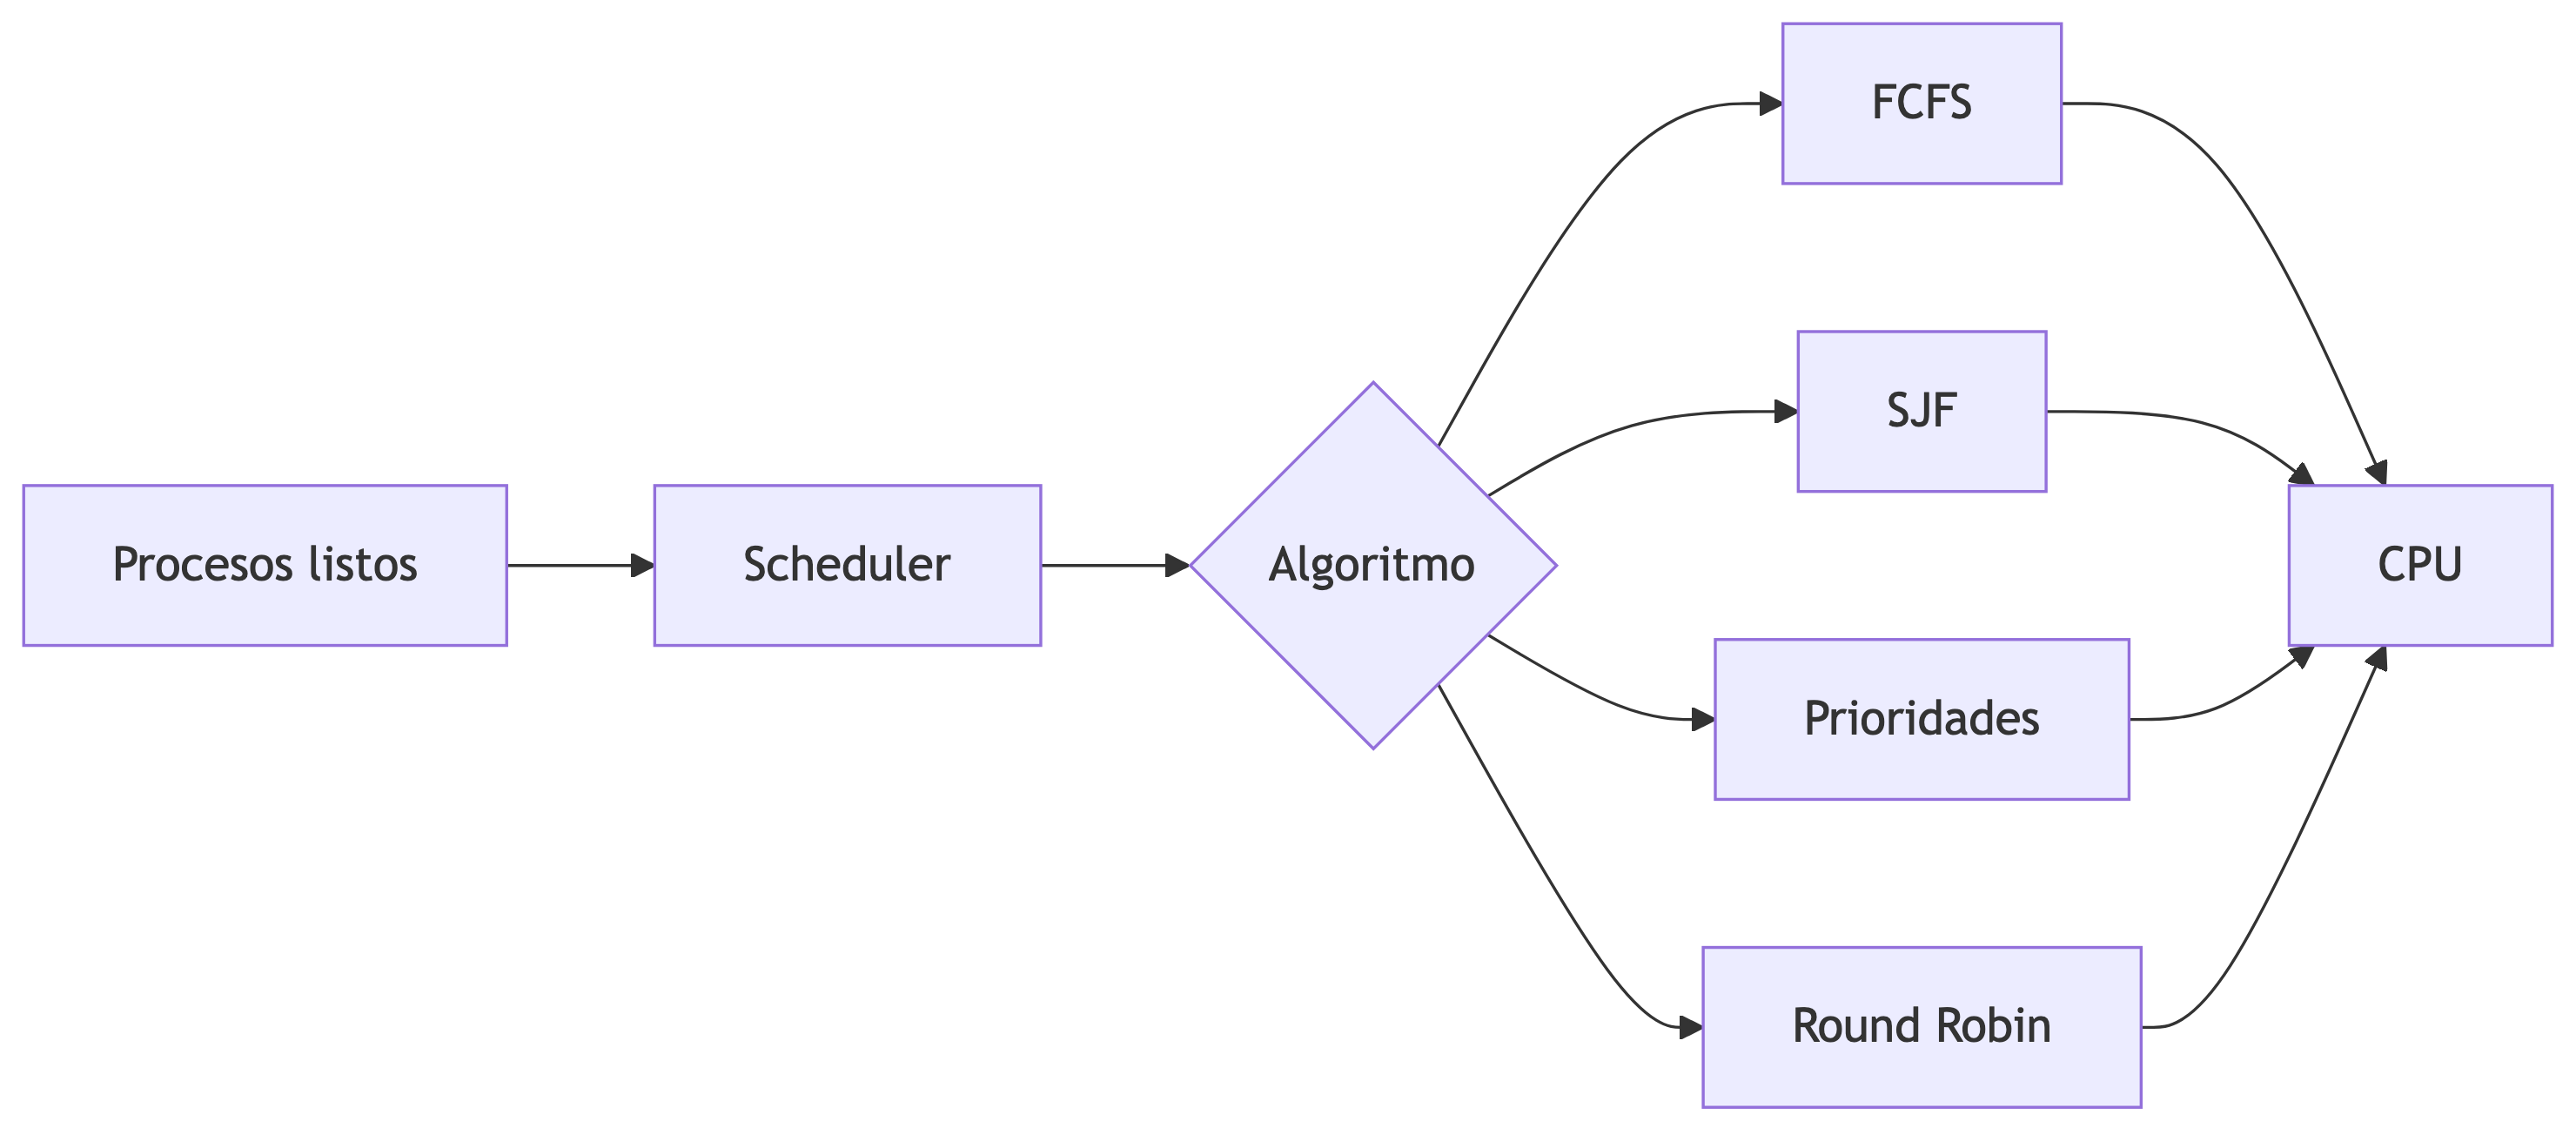
\includegraphics[width=9.06in,height=3.98in]{capitulos/06_algoritmos_de_planificacion_files/figure-latex/mermaid-figure-2.png}

\begin{tcolorbox}[enhanced jigsaw, arc=.35mm, bottomrule=.15mm, bottomtitle=1mm, breakable, colback=white, colbacktitle=quarto-callout-tip-color!10!white, colframe=quarto-callout-tip-color-frame, coltitle=black, left=2mm, leftrule=.75mm, opacityback=0, opacitybacktitle=0.6, rightrule=.15mm, title=\textcolor{quarto-callout-tip-color}{\faLightbulb}\hspace{0.5em}{Idea clave}, titlerule=0mm, toprule=.15mm, toptitle=1mm]

No existe un algoritmo perfecto.

Cada Sistema Operativo selecciona el algoritmo que mejor se adapta a sus
necesidades.

\end{tcolorbox}

\begin{center}\rule{0.5\linewidth}{0.5pt}\end{center}

\bookmarksetup{startatroot}

\chapter{Conexión con el siguiente
capítulo}\label{conexiuxf3n-con-el-siguiente-capuxedtulo}

En el próximo capítulo estudiaremos las \textbf{capas del Sistema
Operativo} y comprenderemos por qué el \textbf{Kernel} es considerado el
corazón del sistema.

\bookmarksetup{startatroot}

\chapter{Capítulo 7. Del hardware al usuario: comprendiendo las capas
del Sistema
Operativo}\label{capuxedtulo-7.-del-hardware-al-usuario-comprendiendo-las-capas-del-sistema-operativo}

\bookmarksetup{startatroot}

\chapter{Capítulo 7. Capas del Sistema
Operativo}\label{capuxedtulo-7.-capas-del-sistema-operativo}

\section{Relación con la clase
anterior}\label{relaciuxf3n-con-la-clase-anterior-1}

En el capítulo anterior aprendimos que el \textbf{Scheduler} decide qué
proceso utilizará el procesador y que el \textbf{Kernel} coordina esa
decisión.

Ahora responderemos una nueva pregunta:

\begin{quote}
\textbf{¿Qué ocurre dentro de una computadora desde que hacemos doble
clic sobre una aplicación hasta que aparece en pantalla?}
\end{quote}

Esta pregunta nos permitirá comprender cómo trabajan juntas las
diferentes capas de un Sistema Operativo.

\begin{center}\rule{0.5\linewidth}{0.5pt}\end{center}

\bookmarksetup{startatroot}

\chapter{Objetivos de aprendizaje}\label{objetivos-de-aprendizaje-5}

Al finalizar este capítulo serás capaz de:

\begin{itemize}
\tightlist
\item
  Comprender la organización por capas de un Sistema Operativo.
\item
  Explicar la función de cada capa.
\item
  Identificar el papel del Kernel dentro de esa arquitectura.
\item
  Relacionar las capas con acciones que realizamos diariamente en una
  computadora.
\end{itemize}

\begin{center}\rule{0.5\linewidth}{0.5pt}\end{center}

\bookmarksetup{startatroot}

\chapter{Motivación}\label{motivaciuxf3n-1}

Todos los días abrimos aplicaciones como:

\begin{itemize}
\tightlist
\item
  Google Chrome
\item
  Microsoft Word
\item
  Visual Studio Code
\item
  Spotify
\end{itemize}

La aplicación aparece en pocos segundos.

Pero\ldots{}

\begin{itemize}
\tightlist
\item
  ¿Quién encuentra el programa en el disco?
\item
  ¿Quién reserva memoria para ejecutarlo?
\item
  ¿Quién se comunica con el teclado y el mouse?
\item
  ¿Quién envía la imagen al monitor?
\item
  ¿Quién controla realmente todo el proceso?
\end{itemize}

La respuesta está en las \textbf{capas del Sistema Operativo}.

\begin{tcolorbox}[enhanced jigsaw, arc=.35mm, bottomrule=.15mm, bottomtitle=1mm, breakable, colback=white, colbacktitle=quarto-callout-note-color!10!white, colframe=quarto-callout-note-color-frame, coltitle=black, left=2mm, leftrule=.75mm, opacityback=0, opacitybacktitle=0.6, rightrule=.15mm, title=\textcolor{quarto-callout-note-color}{\faInfo}\hspace{0.5em}{Pregunta detonadora}, titlerule=0mm, toprule=.15mm, toptitle=1mm]

Cuando haces doble clic sobre una aplicación, ¿qué sucede dentro de la
computadora antes de que aparezca la ventana?

Al finalizar este capítulo podrás responder esa pregunta paso a paso.

\end{tcolorbox}

\begin{center}\rule{0.5\linewidth}{0.5pt}\end{center}

\bookmarksetup{startatroot}

\chapter{Un viaje por el Sistema
Operativo}\label{un-viaje-por-el-sistema-operativo}

Durante esta clase seguiremos el recorrido que realiza una solicitud
desde el usuario hasta el hardware.

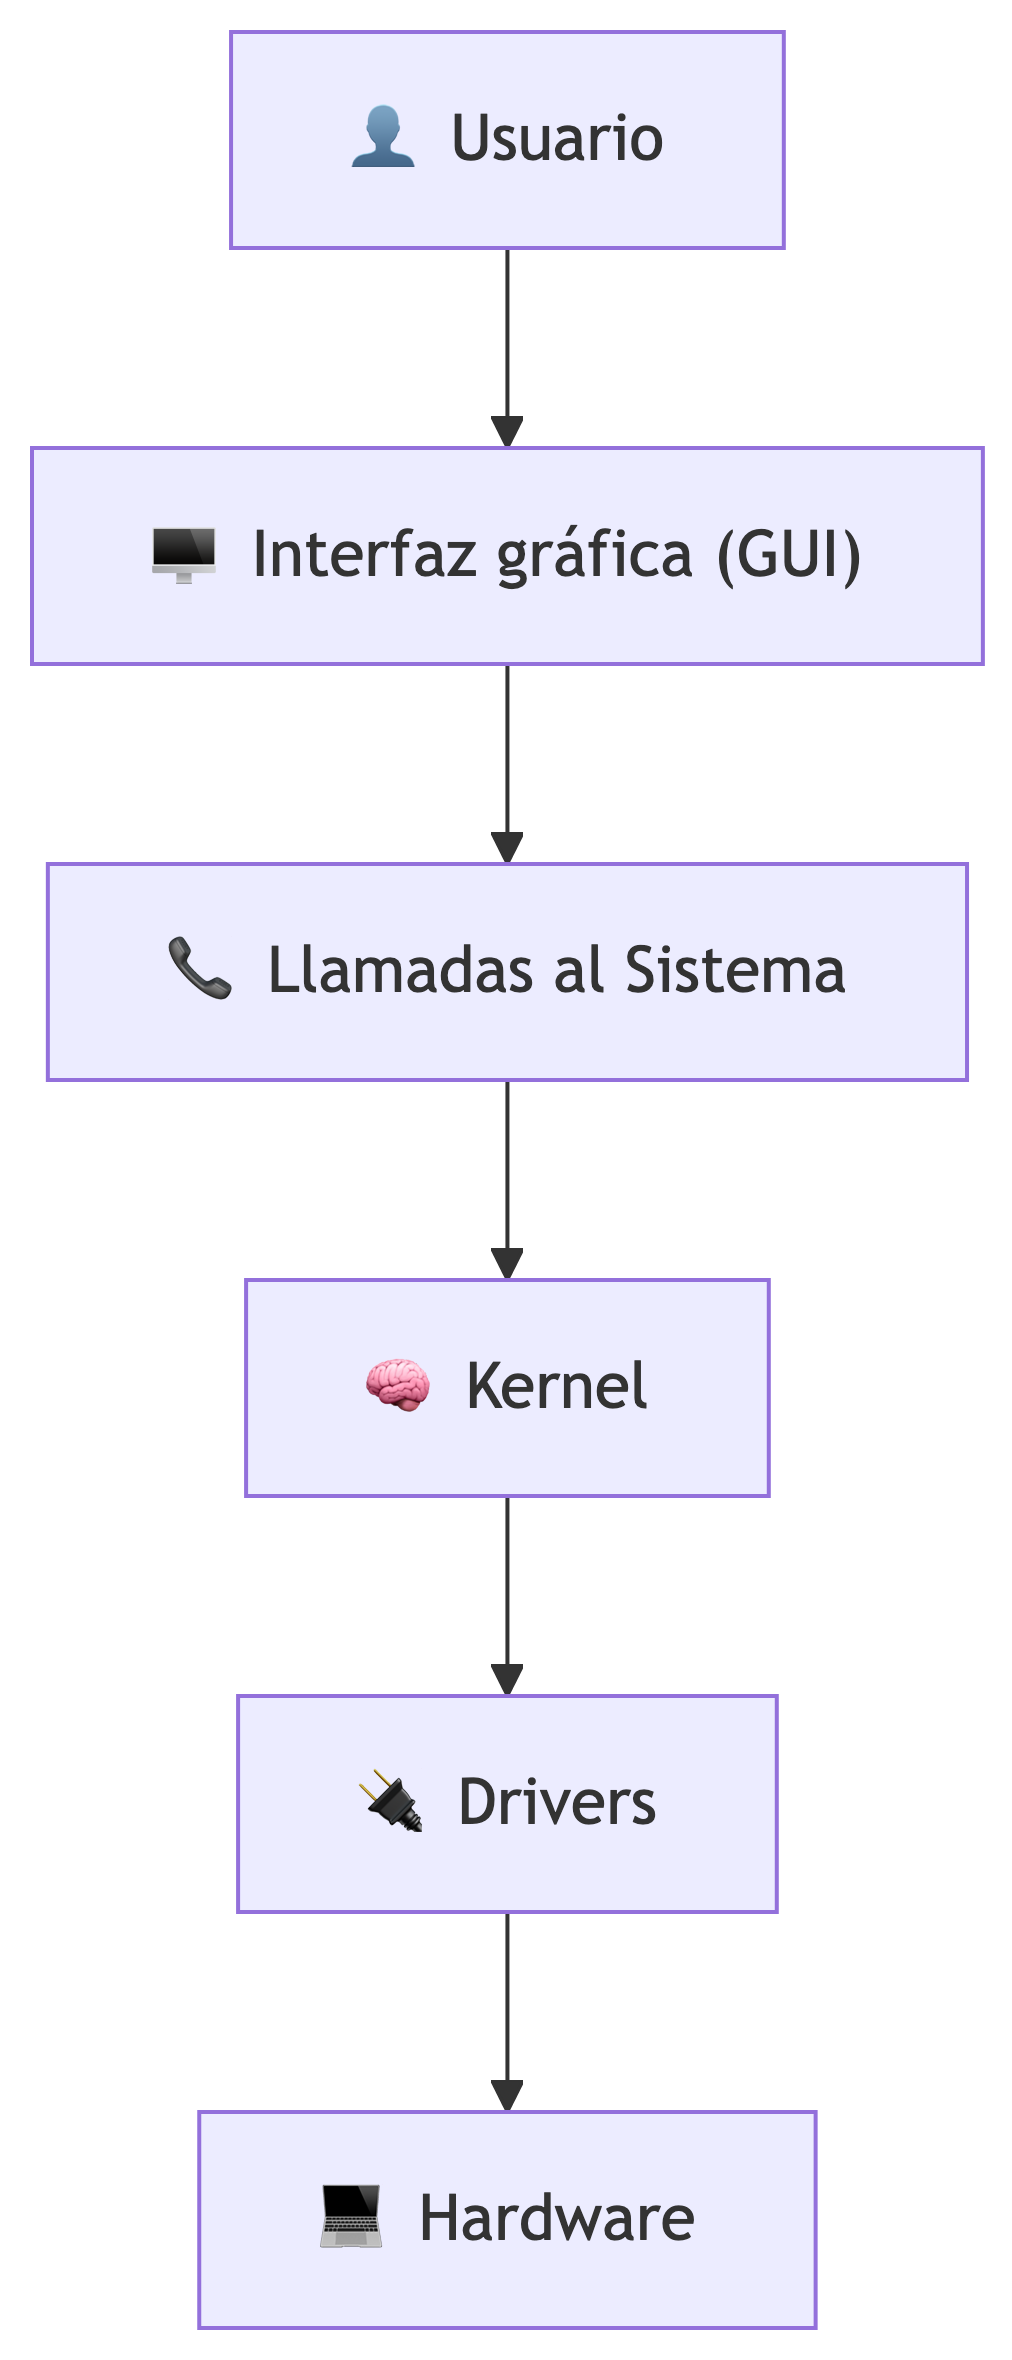
\includegraphics[width=2.64in,height=6.15in]{capitulos/07_capas_del_sistema_operativo_files/figure-latex/mermaid-figure-1.png}

Observa que el usuario nunca se comunica directamente con el hardware.

Siempre existe una cadena de componentes que trabajan coordinadamente.

\begin{center}\rule{0.5\linewidth}{0.5pt}\end{center}

\bookmarksetup{startatroot}

\chapter{¿Por qué organizar el Sistema Operativo por
capas?}\label{por-quuxe9-organizar-el-sistema-operativo-por-capas}

Dividir el Sistema Operativo en capas ofrece varias ventajas.

\begin{itemize}
\tightlist
\item
  Cada capa tiene una responsabilidad específica.
\item
  Facilita el mantenimiento del sistema.
\item
  Reduce errores.
\item
  Permite actualizar componentes sin modificar todo el Sistema
  Operativo.
\item
  Hace posible reutilizar código.
\end{itemize}

Piensa en un edificio.

Cada piso tiene una función distinta, pero todos trabajan juntos para
que el edificio funcione correctamente.

Con un Sistema Operativo ocurre exactamente lo mismo.

\begin{center}\rule{0.5\linewidth}{0.5pt}\end{center}

\bookmarksetup{startatroot}

\chapter{¿Qué aprenderemos en este
capítulo?}\label{quuxe9-aprenderemos-en-este-capuxedtulo-1}

En las siguientes secciones estudiaremos:

\begin{enumerate}
\def\labelenumi{\arabic{enumi}.}
\tightlist
\item
  La arquitectura por capas.
\item
  La función de cada capa.
\item
  El Kernel como corazón del Sistema Operativo.
\item
  Los tipos de Kernel.
\item
  Un caso práctico siguiendo el recorrido de una aplicación desde el
  usuario hasta el hardware.
\end{enumerate}

\begin{center}\rule{0.5\linewidth}{0.5pt}\end{center}

\bookmarksetup{startatroot}

\chapter{Preparándonos para la siguiente
sección}\label{preparuxe1ndonos-para-la-siguiente-secciuxf3n-1}

Ya conocemos el recorrido general.

Ahora estudiaremos cada una de las capas comenzando desde la más cercana
al usuario hasta llegar al \textbf{Kernel}, el componente más importante
del Sistema Operativo.

\bookmarksetup{startatroot}

\chapter{Conociendo las capas del Sistema
Operativo}\label{conociendo-las-capas-del-sistema-operativo}

En la sección anterior vimos que una solicitud recorre varias capas
antes de llegar al hardware.

Ahora estudiaremos cada una de ellas para comprender su función.

\section{Vista general}\label{vista-general}

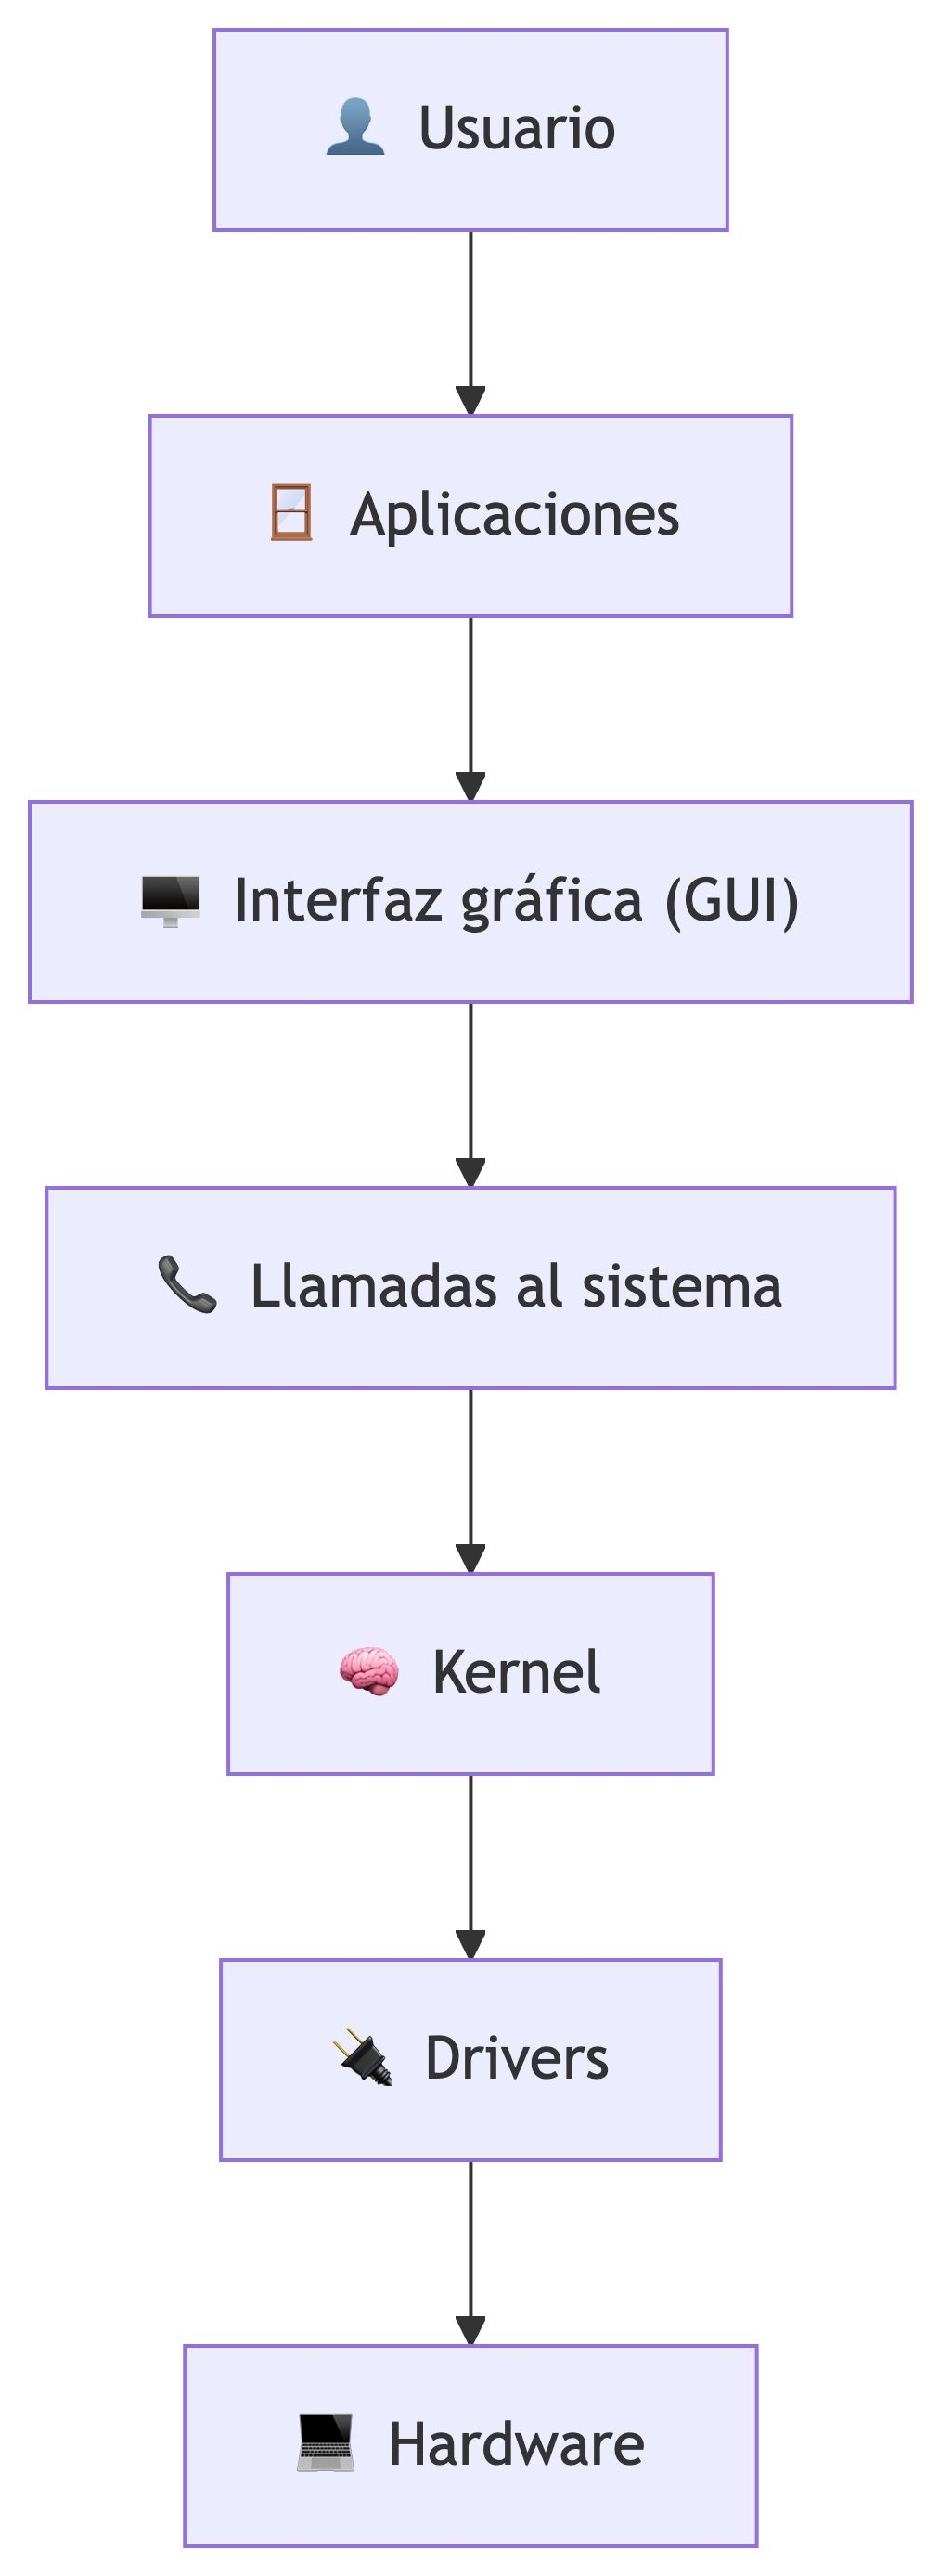
\includegraphics[width=2.64in,height=7.23in]{capitulos/07_capas_del_sistema_operativo_files/figure-latex/mermaid-figure-9.png}

Cada capa tiene una responsabilidad específica y colabora con las demás.

\begin{center}\rule{0.5\linewidth}{0.5pt}\end{center}

\bookmarksetup{startatroot}

\chapter{Capa 1. Usuario}\label{capa-1.-usuario}

Es la persona que utiliza el computador.

Sus acciones son sencillas:

\begin{itemize}
\tightlist
\item
  Hacer clic.
\item
  Escribir con el teclado.
\item
  Abrir un programa.
\item
  Guardar un archivo.
\end{itemize}

El usuario nunca controla directamente el hardware.

\begin{center}\rule{0.5\linewidth}{0.5pt}\end{center}

\bookmarksetup{startatroot}

\chapter{Capa 2. Aplicaciones}\label{capa-2.-aplicaciones}

Son los programas que utilizamos diariamente.

Ejemplos:

\begin{itemize}
\tightlist
\item
  Google Chrome
\item
  Microsoft Word
\item
  Visual Studio Code
\item
  VLC
\end{itemize}

Las aplicaciones solicitan servicios al Sistema Operativo, pero no
acceden directamente al disco, la memoria o el procesador.

\begin{tcolorbox}[enhanced jigsaw, arc=.35mm, bottomrule=.15mm, bottomtitle=1mm, breakable, colback=white, colbacktitle=quarto-callout-note-color!10!white, colframe=quarto-callout-note-color-frame, coltitle=black, left=2mm, leftrule=.75mm, opacityback=0, opacitybacktitle=0.6, rightrule=.15mm, title=\textcolor{quarto-callout-note-color}{\faInfo}\hspace{0.5em}{Idea importante}, titlerule=0mm, toprule=.15mm, toptitle=1mm]

Las aplicaciones dependen del Sistema Operativo para utilizar los
recursos del computador.

\end{tcolorbox}

\begin{center}\rule{0.5\linewidth}{0.5pt}\end{center}

\bookmarksetup{startatroot}

\chapter{Capa 3. Interfaz gráfica
(GUI)}\label{capa-3.-interfaz-gruxe1fica-gui}

La GUI permite que el usuario interactúe mediante:

\begin{itemize}
\tightlist
\item
  Ventanas.
\item
  Botones.
\item
  Menús.
\item
  Iconos.
\end{itemize}

Gracias a ella no es necesario escribir comandos para realizar la
mayoría de las tareas.

\begin{center}\rule{0.5\linewidth}{0.5pt}\end{center}

\bookmarksetup{startatroot}

\chapter{Capa 4. Llamadas al Sistema (System
Calls)}\label{capa-4.-llamadas-al-sistema-system-calls}

Cuando una aplicación necesita un recurso, realiza una \textbf{llamada
al sistema}.

Por ejemplo:

\begin{itemize}
\tightlist
\item
  Abrir un archivo.
\item
  Reservar memoria.
\item
  Crear un proceso.
\item
  Imprimir un documento.
\end{itemize}

Estas solicitudes son enviadas al Kernel.

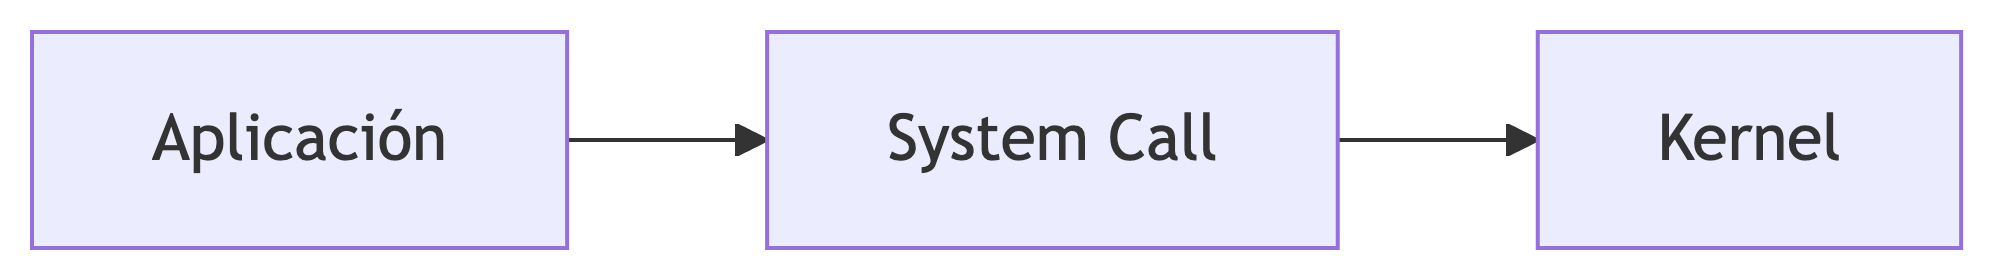
\includegraphics[width=5.19in,height=0.73in]{capitulos/07_capas_del_sistema_operativo_files/figure-latex/mermaid-figure-8.png}

\begin{tcolorbox}[enhanced jigsaw, arc=.35mm, bottomrule=.15mm, bottomtitle=1mm, breakable, colback=white, colbacktitle=quarto-callout-tip-color!10!white, colframe=quarto-callout-tip-color-frame, coltitle=black, left=2mm, leftrule=.75mm, opacityback=0, opacitybacktitle=0.6, rightrule=.15mm, title=\textcolor{quarto-callout-tip-color}{\faLightbulb}\hspace{0.5em}{Reflexiona}, titlerule=0mm, toprule=.15mm, toptitle=1mm]

Cuando haces clic en \textbf{Guardar}, la aplicación no escribe
directamente en el disco.

Primero solicita ese servicio al Sistema Operativo mediante una llamada
al sistema.

\end{tcolorbox}

\begin{center}\rule{0.5\linewidth}{0.5pt}\end{center}

\bookmarksetup{startatroot}

\chapter{¿Qué observamos hasta
ahora?}\label{quuxe9-observamos-hasta-ahora}

Las primeras capas están orientadas al usuario y a las aplicaciones.

Sin embargo, todavía no hemos llegado al componente que realmente
controla el Sistema Operativo.

En la siguiente sección estudiaremos el \textbf{Kernel}, considerado el
corazón del Sistema Operativo.

\bookmarksetup{startatroot}

\chapter{El Kernel: el corazón del Sistema
Operativo}\label{el-kernel-el-corazuxf3n-del-sistema-operativo}

Hasta este momento hemos recorrido varias capas del Sistema Operativo.

Sin embargo, todas ellas dependen de un componente central.

Ese componente recibe el nombre de \textbf{Kernel}.

Si el Sistema Operativo fuera un cuerpo humano, el Kernel sería su
\textbf{corazón y su cerebro}, ya que coordina el funcionamiento de
todos los recursos del computador.

\begin{center}\rule{0.5\linewidth}{0.5pt}\end{center}

\bookmarksetup{startatroot}

\chapter{¿Qué es el Kernel?}\label{quuxe9-es-el-kernel}

El \textbf{Kernel} es la parte más importante del Sistema Operativo.

Es el primer componente que se carga en memoria durante el arranque del
sistema y permanece ejecutándose mientras la computadora está encendida.

Su función principal es actuar como intermediario entre:

\begin{itemize}
\tightlist
\item
  Las aplicaciones.
\item
  El hardware.
\item
  Los dispositivos de entrada y salida.
\item
  La memoria.
\item
  El procesador.
\end{itemize}

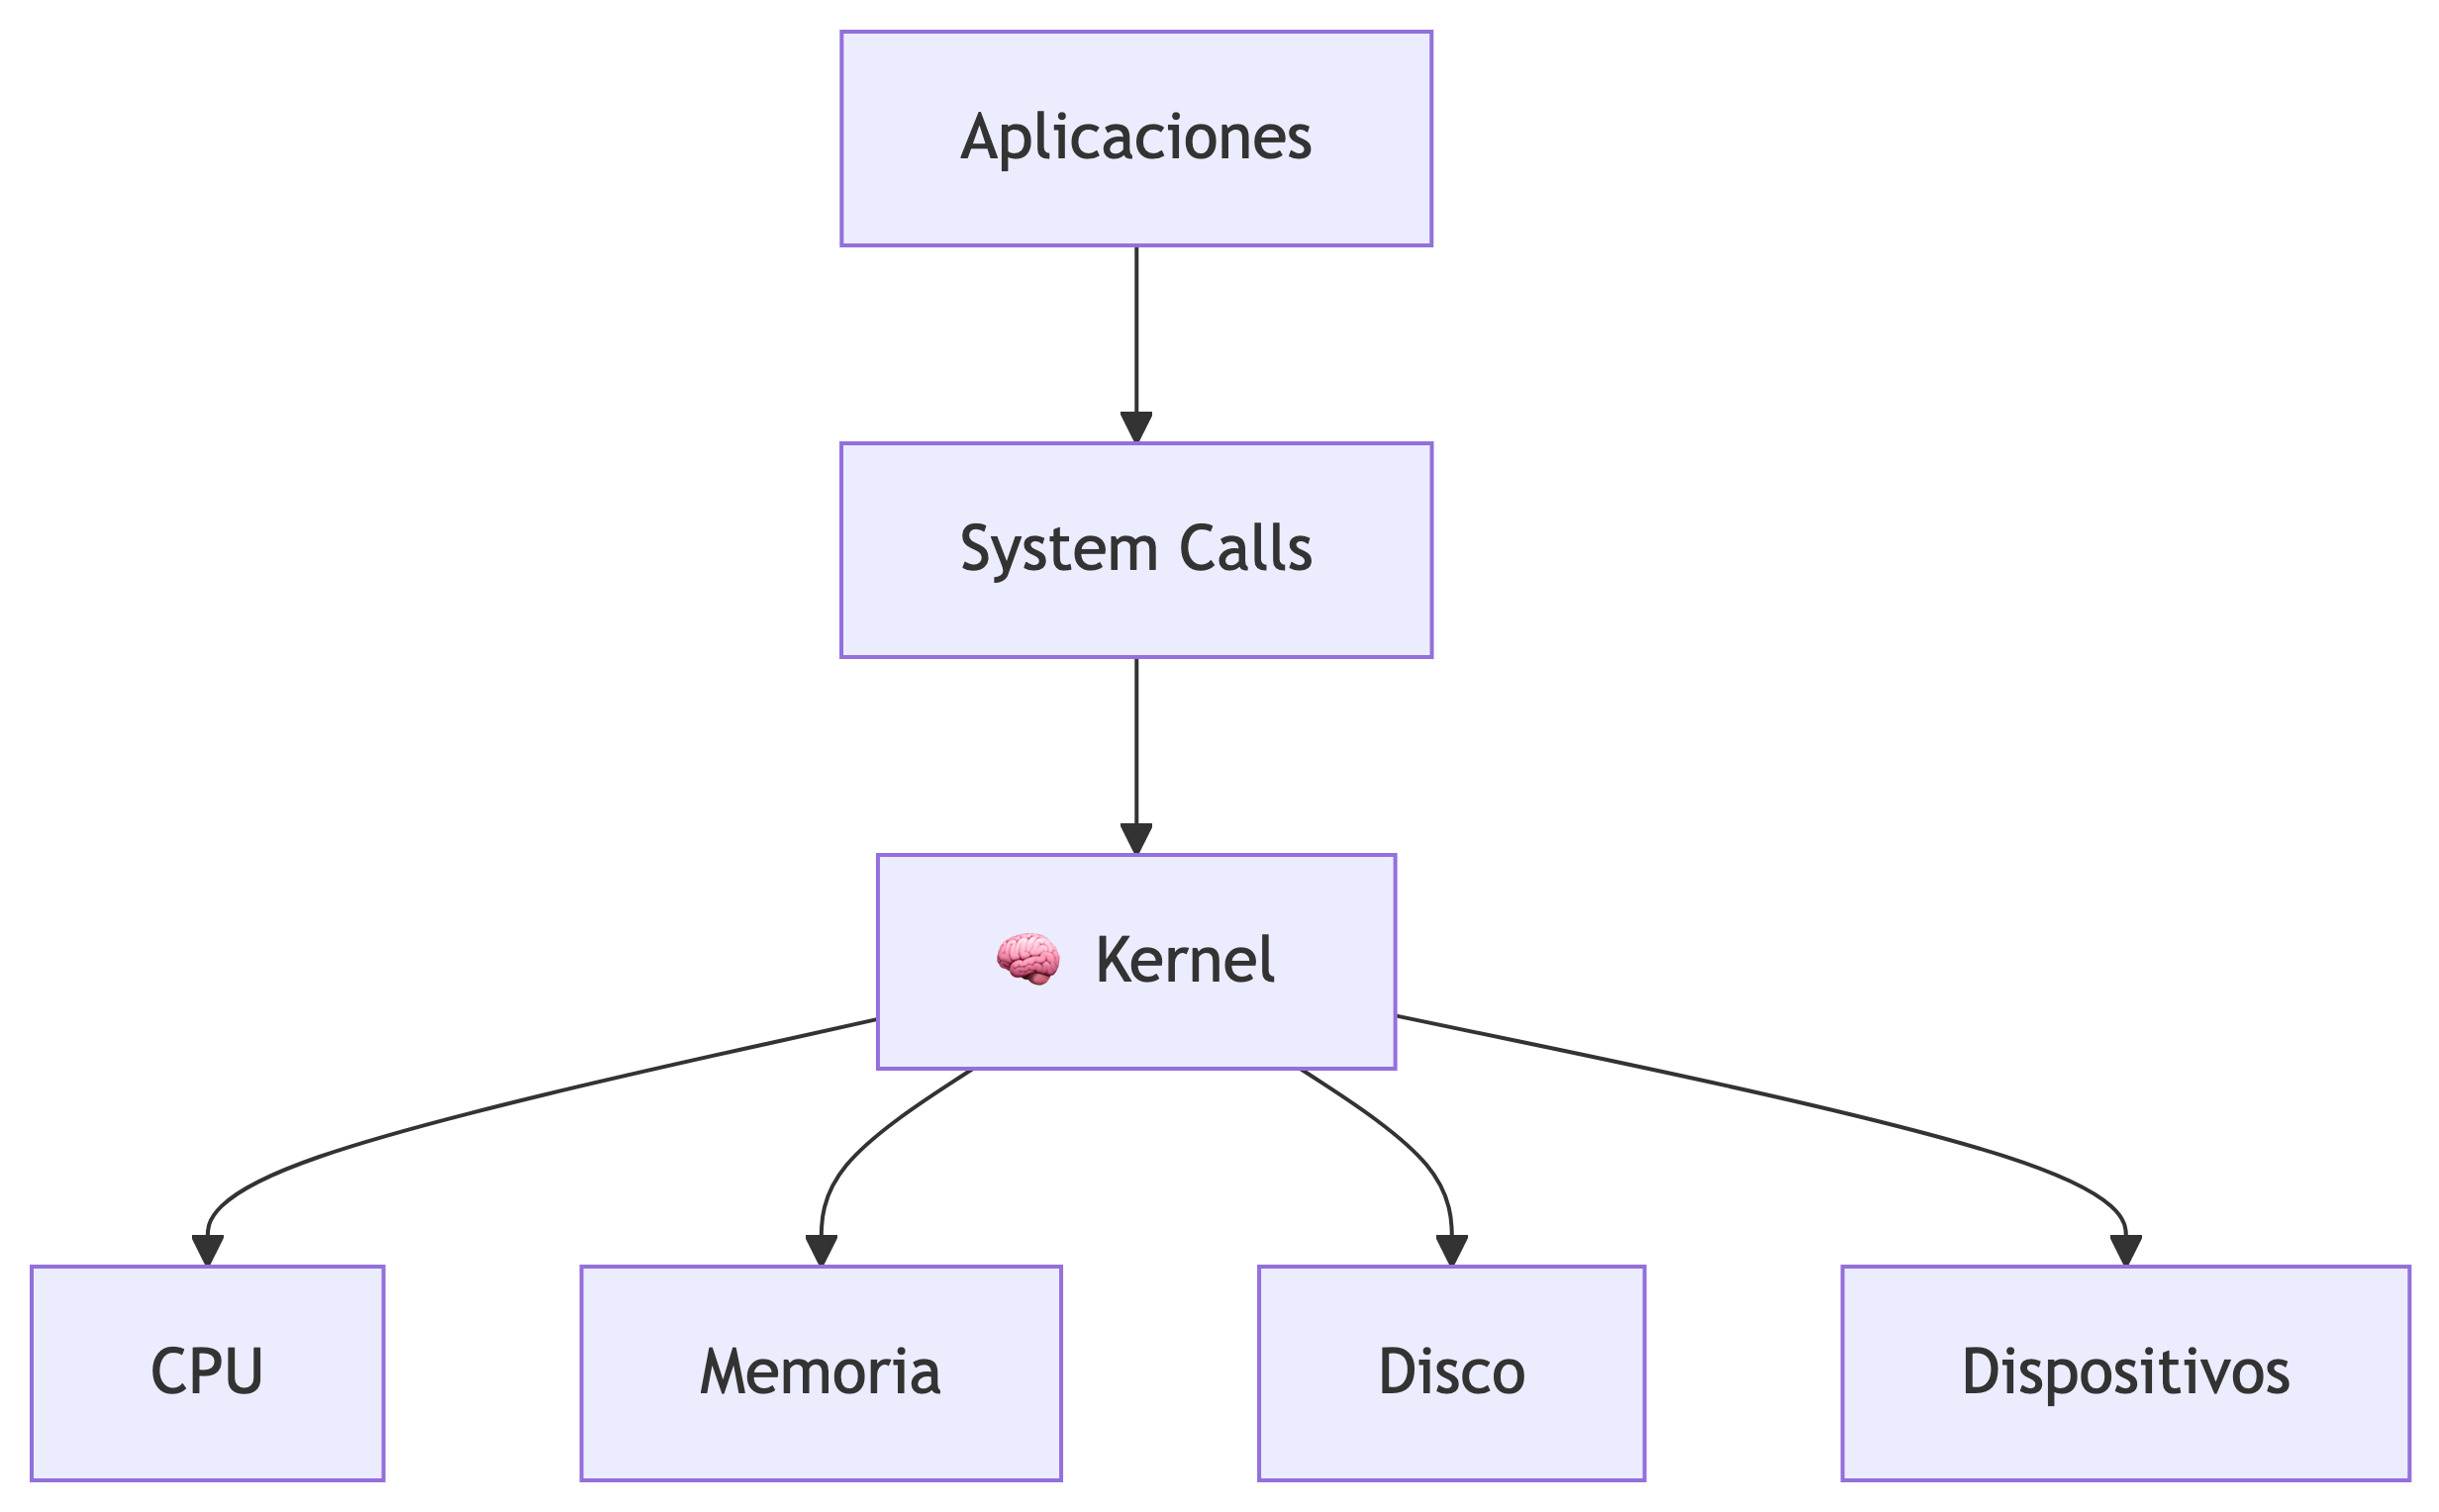
\includegraphics[width=6.42in,height=3.98in]{capitulos/07_capas_del_sistema_operativo_files/figure-latex/mermaid-figure-7.png}

\begin{tcolorbox}[enhanced jigsaw, arc=.35mm, bottomrule=.15mm, bottomtitle=1mm, breakable, colback=white, colbacktitle=quarto-callout-note-color!10!white, colframe=quarto-callout-note-color-frame, coltitle=black, left=2mm, leftrule=.75mm, opacityback=0, opacitybacktitle=0.6, rightrule=.15mm, title=\textcolor{quarto-callout-note-color}{\faInfo}\hspace{0.5em}{Idea clave}, titlerule=0mm, toprule=.15mm, toptitle=1mm]

Las aplicaciones \textbf{nunca acceden directamente al hardware}.

Todas las solicitudes pasan primero por el Kernel.

\end{tcolorbox}

\begin{center}\rule{0.5\linewidth}{0.5pt}\end{center}

\bookmarksetup{startatroot}

\chapter{¿Qué responsabilidades tiene el
Kernel?}\label{quuxe9-responsabilidades-tiene-el-kernel}

El Kernel realiza numerosas tareas al mismo tiempo.

Entre las más importantes se encuentran:

\begin{itemize}
\tightlist
\item
  Administrar los procesos.
\item
  Planificar el uso del procesador.
\item
  Administrar la memoria.
\item
  Controlar los dispositivos mediante los drivers.
\item
  Gestionar el sistema de archivos.
\item
  Atender interrupciones.
\item
  Proteger los recursos del sistema.
\end{itemize}

Observa que muchos de estos temas serán estudiados durante el resto del
curso.

\begin{center}\rule{0.5\linewidth}{0.5pt}\end{center}

\bookmarksetup{startatroot}

\chapter{¿Qué ocurriría si el Kernel no
existiera?}\label{quuxe9-ocurriruxeda-si-el-kernel-no-existiera}

Imagina que una aplicación intenta:

\begin{itemize}
\tightlist
\item
  Leer un archivo.
\item
  Utilizar la impresora.
\item
  Acceder a la memoria.
\item
  Escribir información en el disco.
\end{itemize}

Sin el Kernel:

\begin{itemize}
\tightlist
\item
  Dos programas podrían utilizar la misma memoria.
\item
  Varios procesos intentarían controlar el CPU al mismo tiempo.
\item
  Los dispositivos no podrían coordinarse.
\item
  El sistema sería inestable y probablemente dejaría de funcionar.
\end{itemize}

\begin{tcolorbox}[enhanced jigsaw, arc=.35mm, bottomrule=.15mm, bottomtitle=1mm, breakable, colback=white, colbacktitle=quarto-callout-warning-color!10!white, colframe=quarto-callout-warning-color-frame, coltitle=black, left=2mm, leftrule=.75mm, opacityback=0, opacitybacktitle=0.6, rightrule=.15mm, title=\textcolor{quarto-callout-warning-color}{\faExclamationTriangle}\hspace{0.5em}{Reflexiona}, titlerule=0mm, toprule=.15mm, toptitle=1mm]

El Kernel no solamente administra recursos.

También evita que los programas interfieran entre sí.

\end{tcolorbox}

\begin{center}\rule{0.5\linewidth}{0.5pt}\end{center}

\bookmarksetup{startatroot}

\chapter{Relación con los temas
estudiados}\label{relaciuxf3n-con-los-temas-estudiados}

Observa cómo el Kernel aparece en casi todo lo que hemos aprendido.

{\def\LTcaptype{none} % do not increment counter
\begin{longtable}[]{@{}ll@{}}
\toprule\noalign{}
Tema & Participación del Kernel \\
\midrule\noalign{}
\endhead
\bottomrule\noalign{}
\endlastfoot
Procesos & Los crea y administra \\
Scheduler & Coordina la planificación \\
Dispatcher & Coordina el cambio de contexto \\
Memoria & Reserva y libera espacios \\
Archivos & Controla el acceso al disco \\
Dispositivos & Se comunica mediante drivers \\
\end{longtable}
}

Esto demuestra por qué se le considera el \textbf{corazón del Sistema
Operativo}.

\begin{center}\rule{0.5\linewidth}{0.5pt}\end{center}

\bookmarksetup{startatroot}

\chapter{Preparándonos para la siguiente
sección}\label{preparuxe1ndonos-para-la-siguiente-secciuxf3n-2}

Ya conocemos la importancia del Kernel.

Ahora estudiaremos que \textbf{no todos los Sistemas Operativos utilizan
el mismo tipo de Kernel}.

Analizaremos los modelos:

\begin{itemize}
\tightlist
\item
  Monolítico.
\item
  Microkernel.
\item
  Híbrido.
\end{itemize}

Y conoceremos cuál utiliza Windows, Linux y macOS.

\bookmarksetup{startatroot}

\chapter{Tipos de Kernel}\label{tipos-de-kernel}

En la sección anterior aprendimos que el \textbf{Kernel} es el corazón
del Sistema Operativo.

Sin embargo, no todos los Sistemas Operativos implementan el Kernel de
la misma forma.

Dependiendo de su diseño, existen diferentes arquitecturas.

\begin{center}\rule{0.5\linewidth}{0.5pt}\end{center}

\bookmarksetup{startatroot}

\chapter{Kernel Monolítico}\label{kernel-monoluxedtico}

En un \textbf{Kernel Monolítico}, la mayoría de los servicios del
Sistema Operativo se ejecutan dentro del propio Kernel.

Esto significa que:

\begin{itemize}
\tightlist
\item
  Administración de memoria.
\item
  Sistema de archivos.
\item
  Controladores (drivers).
\item
  Redes.
\item
  Planificación de procesos.
\end{itemize}

trabajan en un mismo espacio del Kernel.

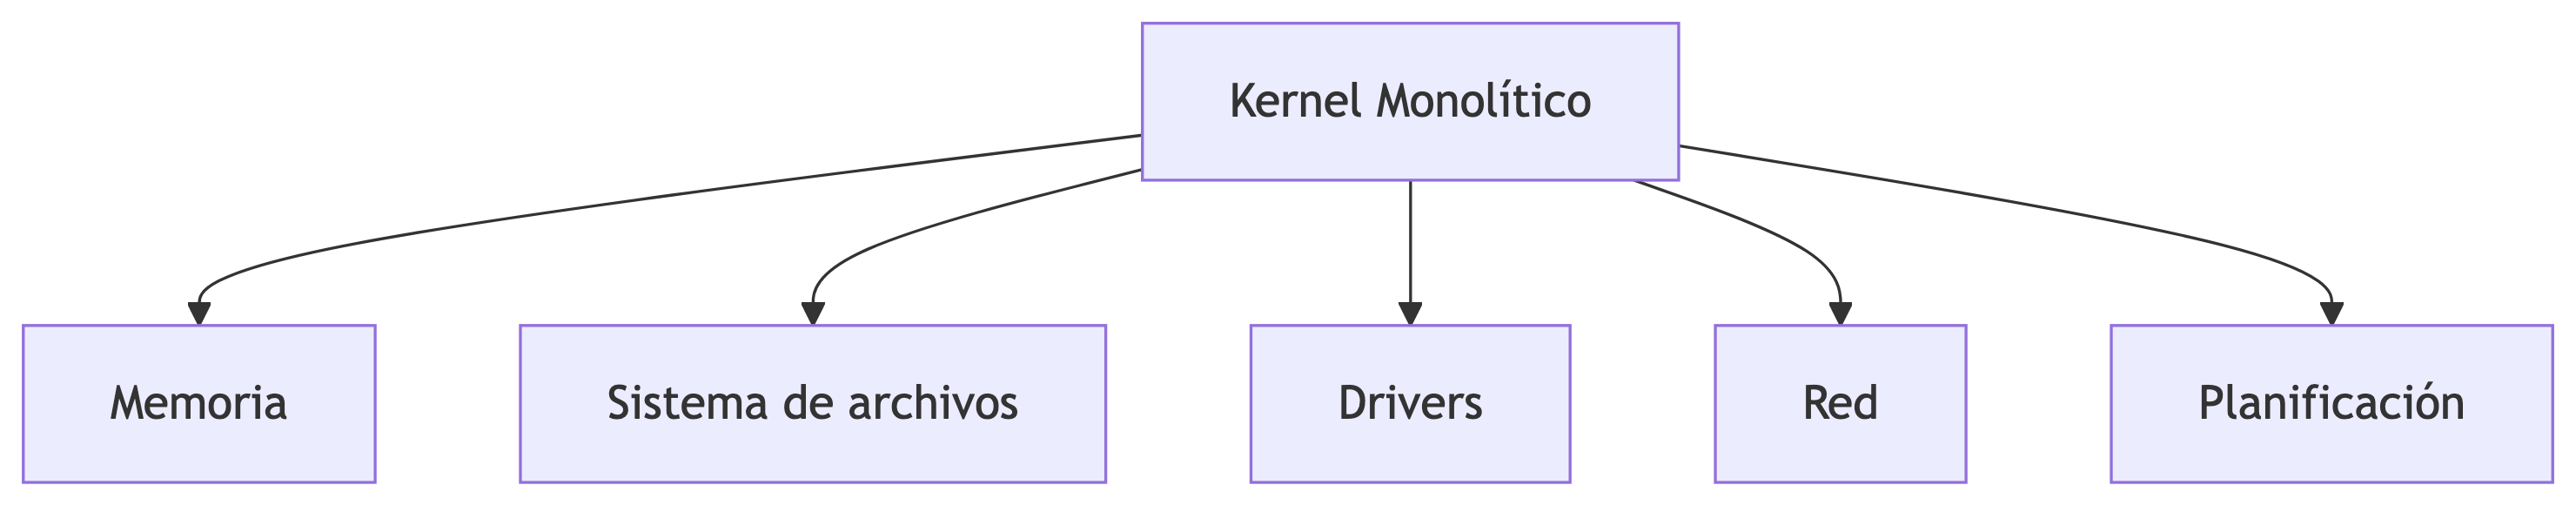
\includegraphics[width=9.24in,height=1.81in]{capitulos/07_capas_del_sistema_operativo_files/figure-latex/mermaid-figure-6.png}

\section{Ventajas}\label{ventajas-7}

\begin{itemize}
\tightlist
\item
  Muy rápido.
\item
  Excelente rendimiento.
\item
  Menor sobrecarga.
\end{itemize}

\section{Desventajas}\label{desventajas-4}

\begin{itemize}
\tightlist
\item
  Un error en un componente puede afectar todo el sistema.
\item
  Mayor complejidad para mantener.
\end{itemize}

Ejemplo: \textbf{Linux}.

\begin{center}\rule{0.5\linewidth}{0.5pt}\end{center}

\bookmarksetup{startatroot}

\chapter{Microkernel}\label{microkernel}

El \textbf{Microkernel} mantiene dentro del Kernel únicamente las
funciones esenciales.

Otros servicios se ejecutan fuera del Kernel como procesos
independientes.

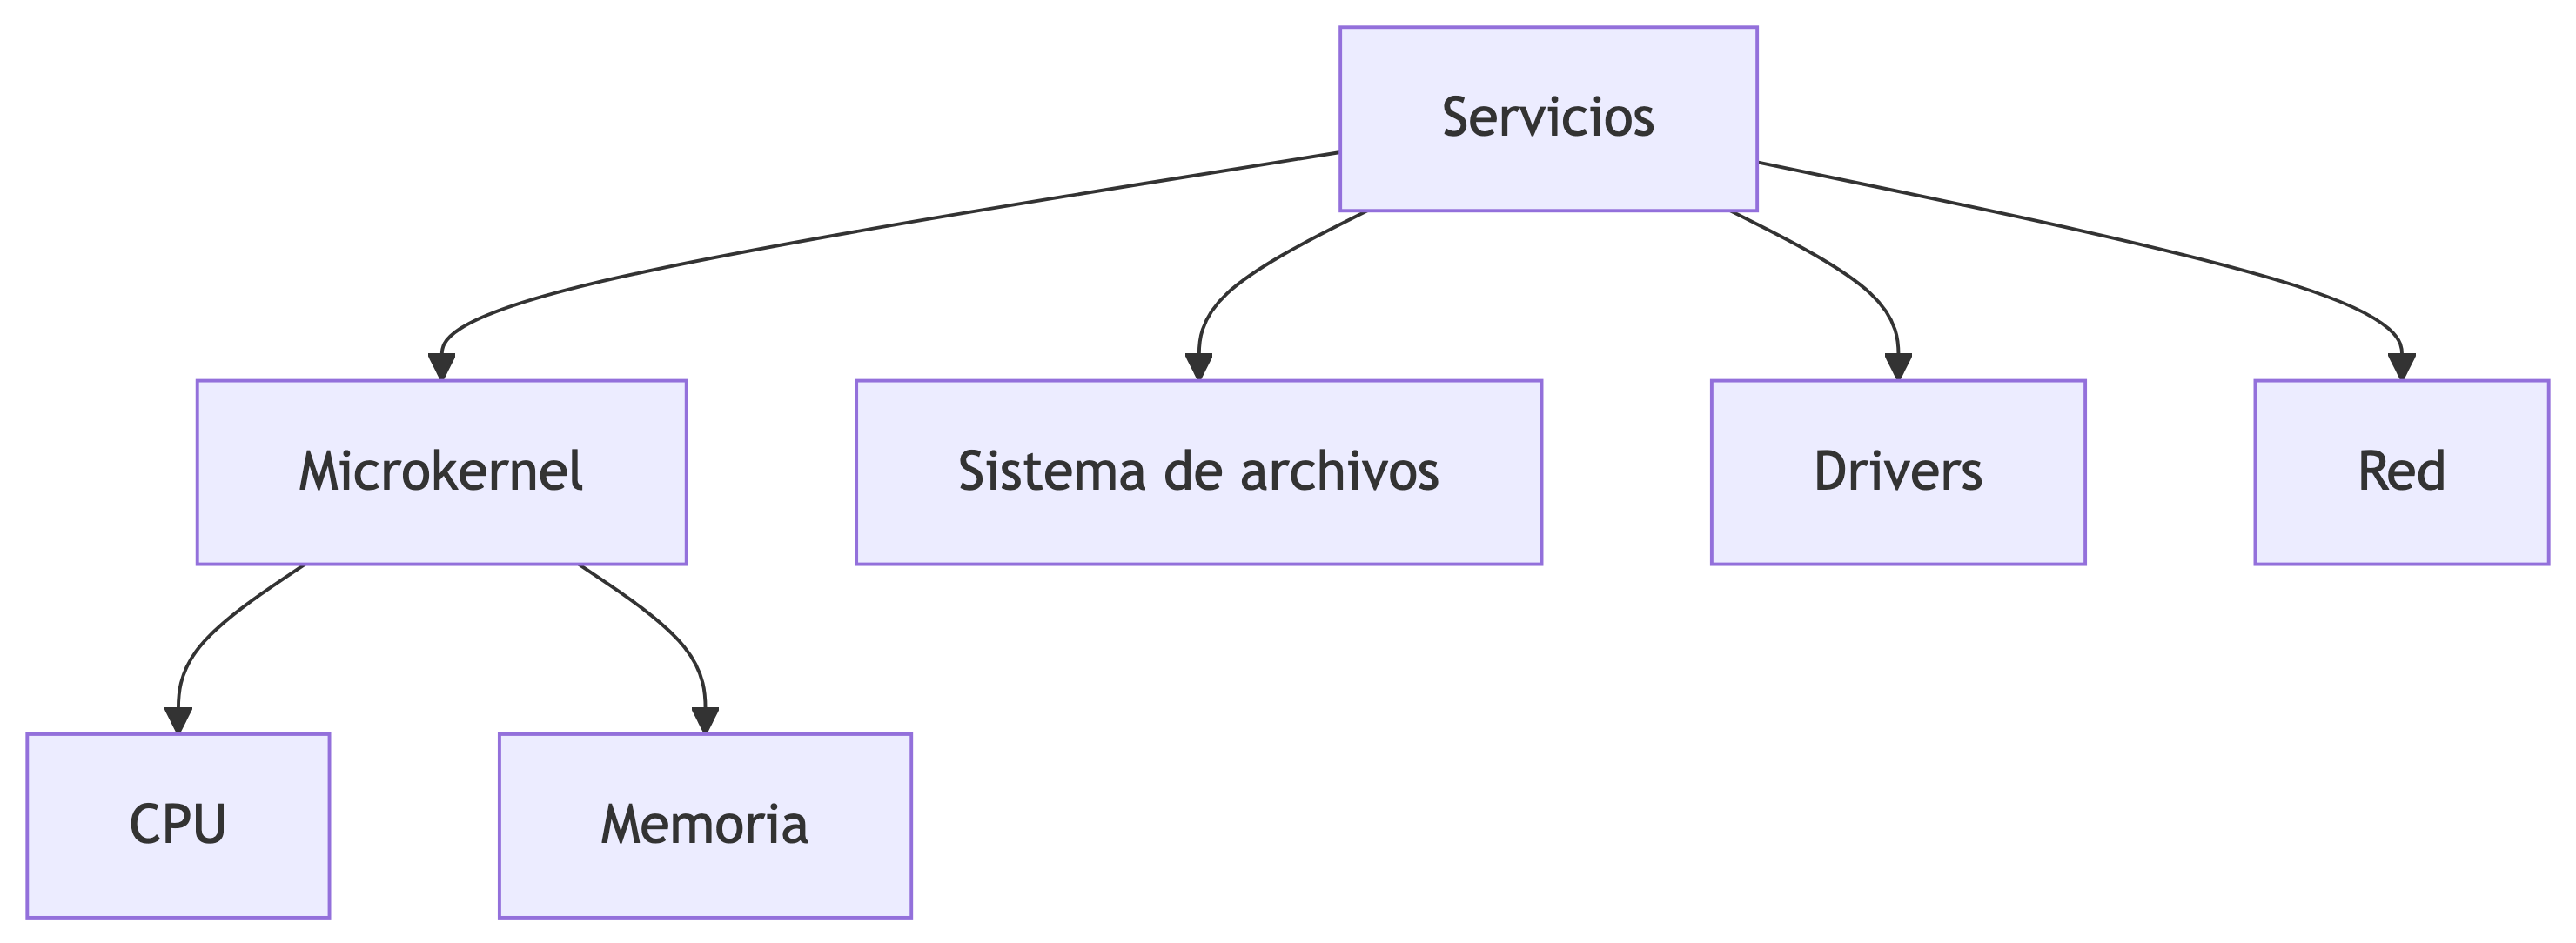
\includegraphics[width=7.89in,height=2.9in]{capitulos/07_capas_del_sistema_operativo_files/figure-latex/mermaid-figure-5.png}

\section{Ventajas}\label{ventajas-8}

\begin{itemize}
\tightlist
\item
  Mayor estabilidad.
\item
  Más seguro.
\item
  Fácil de mantener.
\end{itemize}

\section{Desventajas}\label{desventajas-5}

\begin{itemize}
\tightlist
\item
  Mayor comunicación entre procesos.
\item
  Menor rendimiento que un monolítico.
\end{itemize}

Ejemplo clásico: \textbf{MINIX}.

\begin{center}\rule{0.5\linewidth}{0.5pt}\end{center}

\bookmarksetup{startatroot}

\chapter{Kernel Híbrido}\label{kernel-huxedbrido}

El \textbf{Kernel Híbrido} combina características del Kernel Monolítico
y del Microkernel.

Mantiene servicios importantes dentro del Kernel para mejorar el
rendimiento y deja otros componentes fuera para aumentar la modularidad.

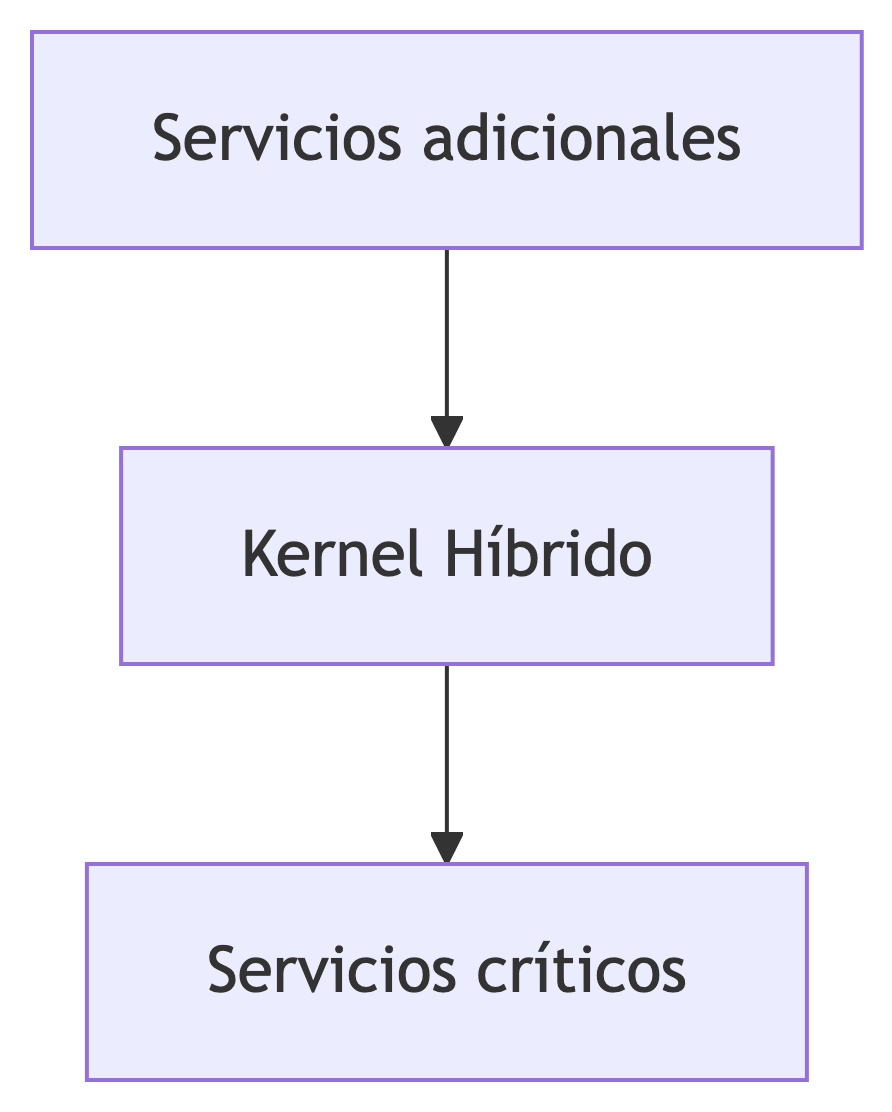
\includegraphics[width=2.33in,height=2.9in]{capitulos/07_capas_del_sistema_operativo_files/figure-latex/mermaid-figure-4.png}

\section{Ventajas}\label{ventajas-9}

\begin{itemize}
\tightlist
\item
  Buen equilibrio entre rendimiento y estabilidad.
\item
  Muy utilizado en sistemas modernos.
\end{itemize}

\section{Desventajas}\label{desventajas-6}

\begin{itemize}
\tightlist
\item
  Arquitectura más compleja.
\end{itemize}

Ejemplos:

\begin{itemize}
\tightlist
\item
  Windows
\item
  macOS
\end{itemize}

\begin{center}\rule{0.5\linewidth}{0.5pt}\end{center}

\bookmarksetup{startatroot}

\chapter{Comparación}\label{comparaciuxf3n-2}

{\def\LTcaptype{none} % do not increment counter
\begin{longtable}[]{@{}llll@{}}
\toprule\noalign{}
Característica & Monolítico & Microkernel & Híbrido \\
\midrule\noalign{}
\endhead
\bottomrule\noalign{}
\endlastfoot
Rendimiento & Alto & Medio & Alto \\
Estabilidad & Media & Alta & Alta \\
Mantenimiento & Difícil & Fácil & Medio \\
Ejemplo & Linux & MINIX & Windows / macOS \\
\end{longtable}
}

\begin{tcolorbox}[enhanced jigsaw, arc=.35mm, bottomrule=.15mm, bottomtitle=1mm, breakable, colback=white, colbacktitle=quarto-callout-note-color!10!white, colframe=quarto-callout-note-color-frame, coltitle=black, left=2mm, leftrule=.75mm, opacityback=0, opacitybacktitle=0.6, rightrule=.15mm, title=\textcolor{quarto-callout-note-color}{\faInfo}\hspace{0.5em}{Idea clave}, titlerule=0mm, toprule=.15mm, toptitle=1mm]

No existe un tipo de Kernel perfecto.

Cada arquitectura representa un equilibrio distinto entre
\textbf{rendimiento}, \textbf{seguridad}, \textbf{mantenimiento} y
\textbf{modularidad}.

\end{tcolorbox}

\bookmarksetup{startatroot}

\chapter{Preparándonos para el
cierre}\label{preparuxe1ndonos-para-el-cierre-1}

En la siguiente sección seguiremos el recorrido completo de una
aplicación desde que el usuario hace doble clic hasta que aparece en
pantalla y resumiremos todo lo aprendido en este capítulo.

\bookmarksetup{startatroot}

\chapter{Caso integrador: ¿Qué ocurre cuando abrimos una
aplicación?}\label{caso-integrador-quuxe9-ocurre-cuando-abrimos-una-aplicaciuxf3n}

Llegó el momento de integrar todo lo aprendido.

Imagina que haces doble clic sobre \textbf{Google Chrome}.

A simple vista únicamente aparece una ventana en la pantalla.

Sin embargo, internamente ocurre una secuencia de eventos perfectamente
organizada.

\section{Paso 1. El usuario solicita abrir la
aplicación}\label{paso-1.-el-usuario-solicita-abrir-la-aplicaciuxf3n}

El usuario hace doble clic sobre el icono.

La solicitud llega a la \textbf{Interfaz Gráfica (GUI)}.

\section{Paso 2. La aplicación solicita
servicios}\label{paso-2.-la-aplicaciuxf3n-solicita-servicios}

La aplicación necesita:

\begin{itemize}
\tightlist
\item
  Leer su archivo ejecutable.
\item
  Reservar memoria.
\item
  Crear un proceso.
\item
  Obtener tiempo de CPU.
\end{itemize}

Para ello realiza \textbf{llamadas al sistema (System Calls)}.

\section{Paso 3. El Kernel entra en
acción}\label{paso-3.-el-kernel-entra-en-acciuxf3n}

El Kernel recibe la solicitud y comienza a coordinar todos los recursos
necesarios.

Entre otras tareas:

\begin{itemize}
\tightlist
\item
  Crea el proceso.
\item
  Reserva memoria.
\item
  Consulta el sistema de archivos.
\item
  Coordina el Scheduler.
\item
  Se comunica con los Drivers.
\end{itemize}

\section{Paso 4. Los Drivers controlan el
hardware}\label{paso-4.-los-drivers-controlan-el-hardware}

Los Drivers permiten que el Sistema Operativo se comunique con:

\begin{itemize}
\tightlist
\item
  Disco duro o SSD.
\item
  Tarjeta gráfica.
\item
  Teclado.
\item
  Mouse.
\item
  Monitor.
\end{itemize}

\section{Paso 5. La aplicación aparece en
pantalla}\label{paso-5.-la-aplicaciuxf3n-aparece-en-pantalla}

Cuando todos los recursos están preparados, la ventana finalmente
aparece y el usuario puede comenzar a trabajar.

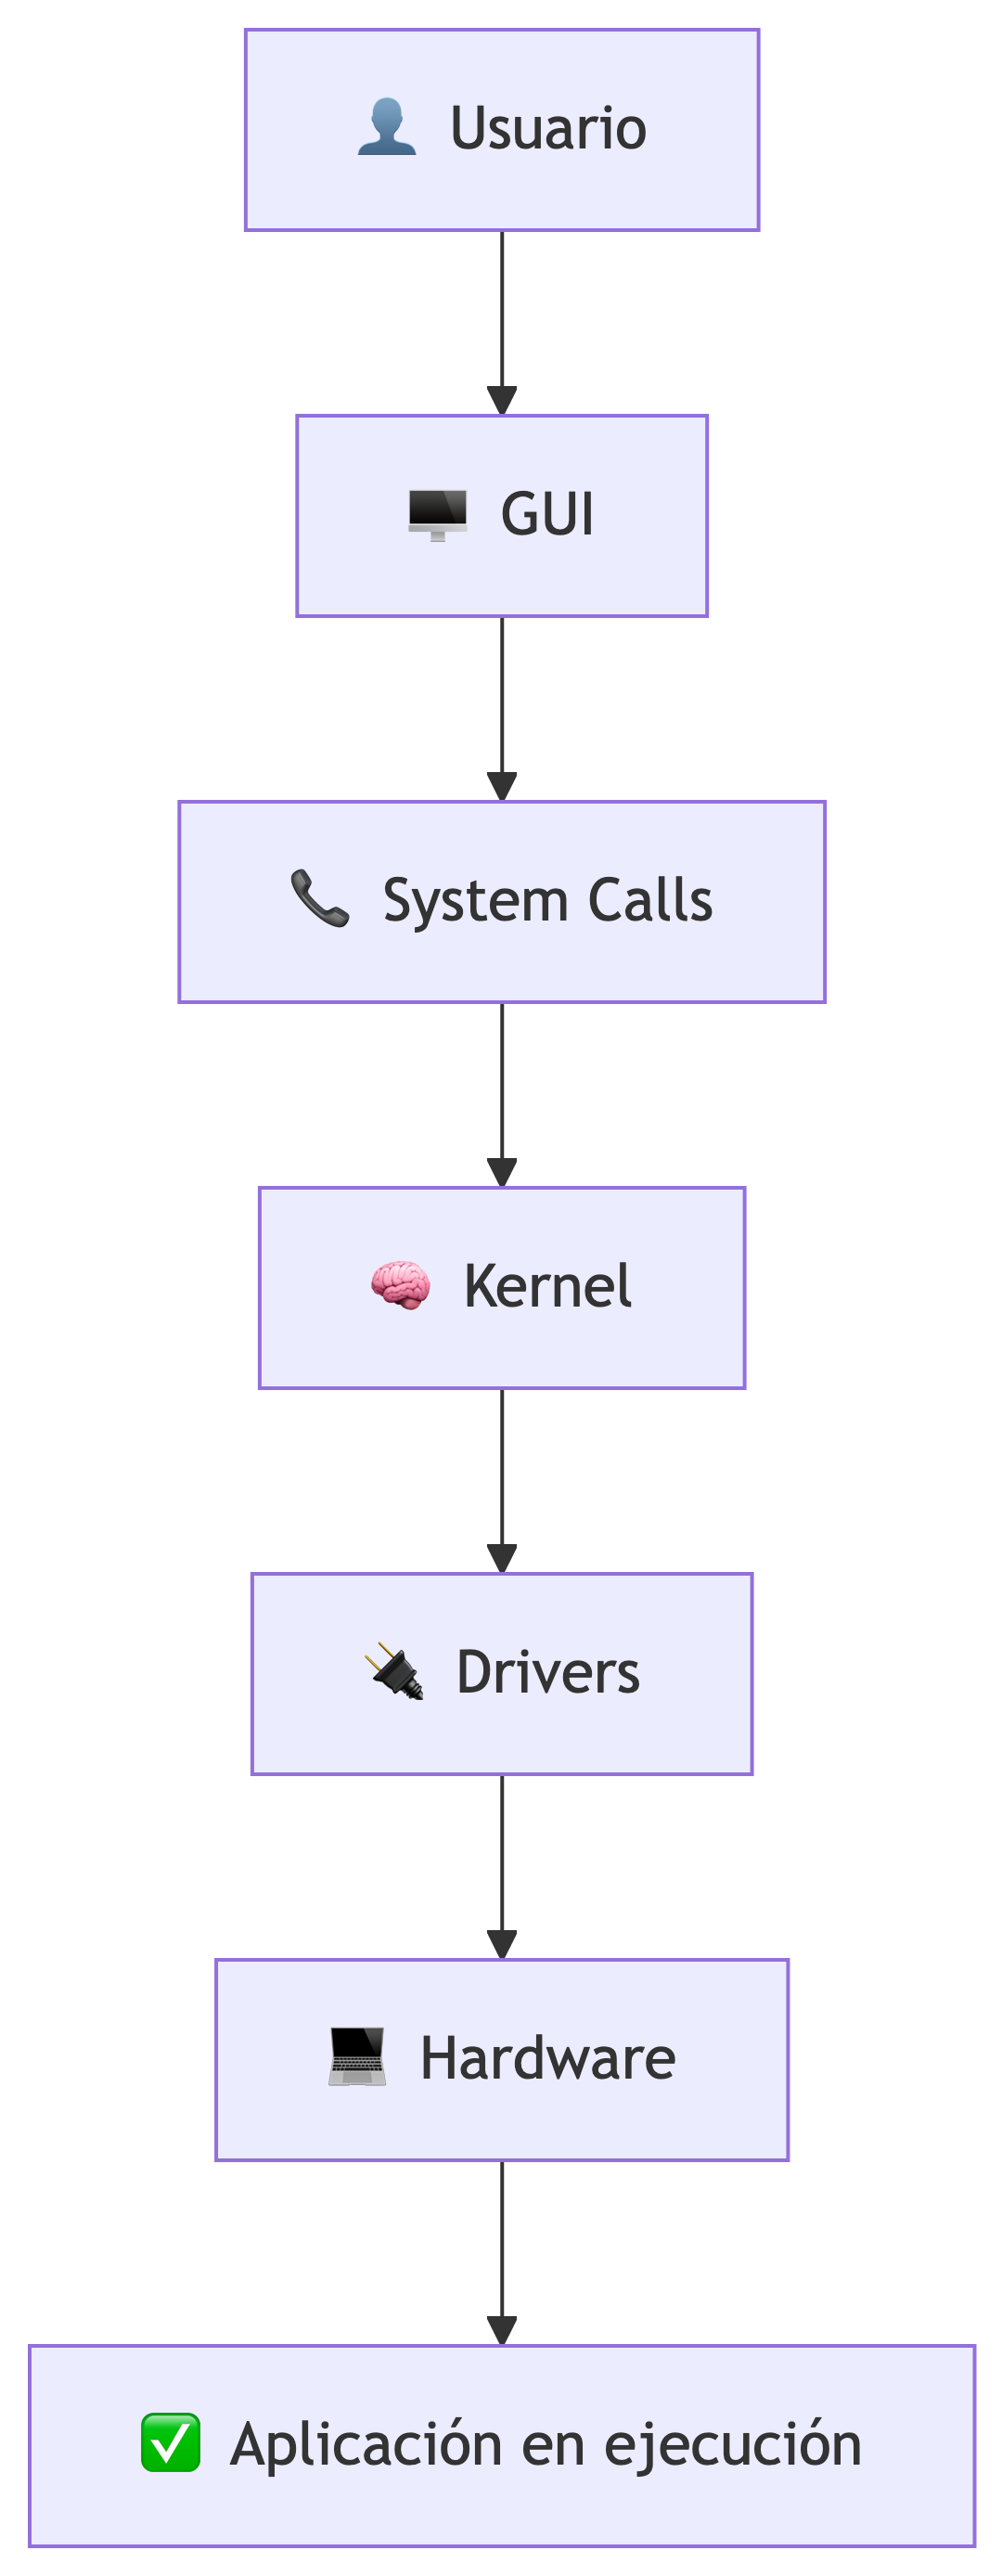
\includegraphics[width=2.82in,height=7.23in]{capitulos/07_capas_del_sistema_operativo_files/figure-latex/mermaid-figure-3.png}

\begin{tcolorbox}[enhanced jigsaw, arc=.35mm, bottomrule=.15mm, bottomtitle=1mm, breakable, colback=white, colbacktitle=quarto-callout-tip-color!10!white, colframe=quarto-callout-tip-color-frame, coltitle=black, left=2mm, leftrule=.75mm, opacityback=0, opacitybacktitle=0.6, rightrule=.15mm, title=\textcolor{quarto-callout-tip-color}{\faLightbulb}\hspace{0.5em}{Idea clave}, titlerule=0mm, toprule=.15mm, toptitle=1mm]

El usuario observa un único clic.

El Sistema Operativo coordina cientos de operaciones en apenas unos
milisegundos.

\end{tcolorbox}

\begin{center}\rule{0.5\linewidth}{0.5pt}\end{center}

\bookmarksetup{startatroot}

\chapter{Autoevaluación}\label{autoevaluaciuxf3n-4}

\begin{enumerate}
\def\labelenumi{\arabic{enumi}.}
\tightlist
\item
  ¿Cuál es la función principal del Kernel?
\item
  ¿Qué capa recibe directamente las solicitudes de las aplicaciones?
\item
  ¿Qué son las System Calls?
\item
  ¿Por qué las aplicaciones no acceden directamente al hardware?
\item
  ¿Cuál es la función de los Drivers?
\item
  ¿Qué diferencia existe entre un Kernel Monolítico y un Microkernel?
\item
  ¿Qué ventajas ofrece un Kernel Híbrido?
\item
  ¿Qué ocurriría si el Kernel dejara de funcionar?
\item
  ¿Por qué decimos que el Kernel es el corazón del Sistema Operativo?
\item
  Describe el recorrido que sigue una solicitud desde el usuario hasta
  el hardware.
\end{enumerate}

\begin{center}\rule{0.5\linewidth}{0.5pt}\end{center}

\bookmarksetup{startatroot}

\chapter{Resumen del capítulo}\label{resumen-del-capuxedtulo-1}

Durante este capítulo comprendimos que un Sistema Operativo está
organizado por capas para facilitar la administración de los recursos
del computador.

Aprendimos que:

\begin{itemize}
\tightlist
\item
  El usuario interactúa con las aplicaciones.
\item
  Las aplicaciones solicitan servicios mediante llamadas al sistema.
\item
  El Kernel coordina todos los recursos.
\item
  Los Drivers permiten controlar el hardware.
\item
  Existen diferentes arquitecturas de Kernel según las necesidades del
  sistema.
\end{itemize}

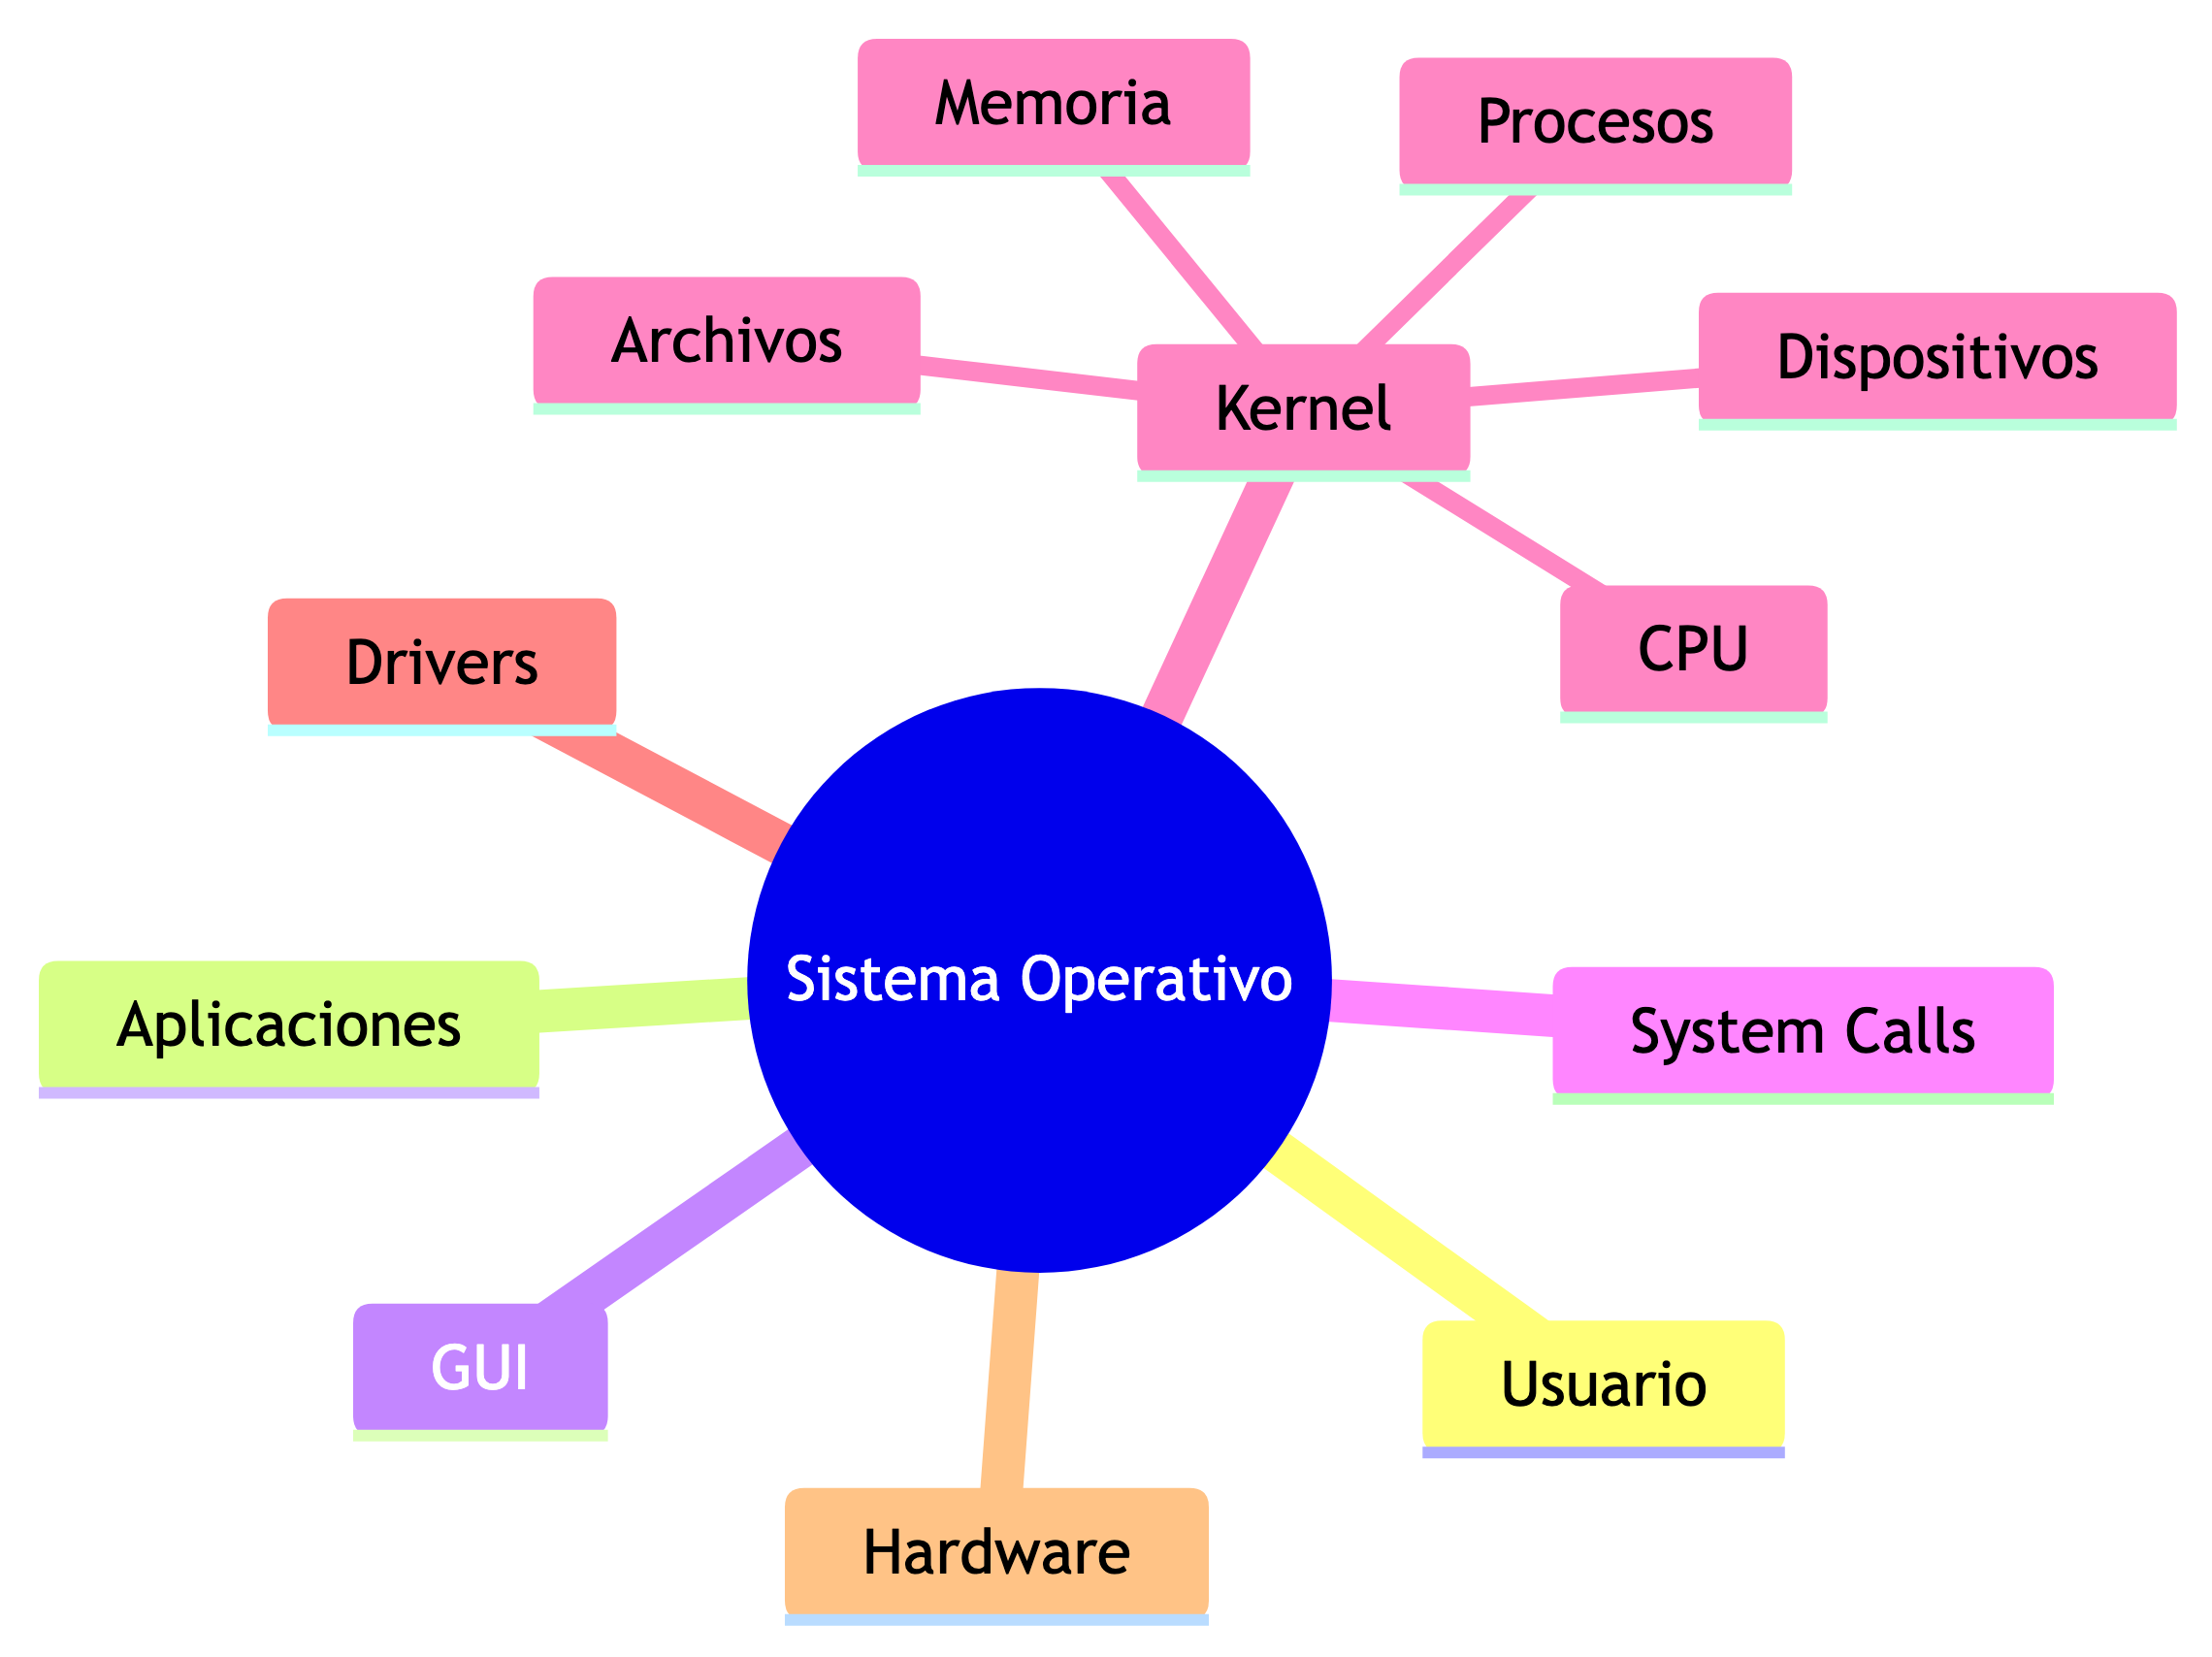
\includegraphics[width=5.95in,height=4.45in]{capitulos/07_capas_del_sistema_operativo_files/figure-latex/mermaid-figure-2.png}

\begin{tcolorbox}[enhanced jigsaw, arc=.35mm, bottomrule=.15mm, bottomtitle=1mm, breakable, colback=white, colbacktitle=quarto-callout-note-color!10!white, colframe=quarto-callout-note-color-frame, coltitle=black, left=2mm, leftrule=.75mm, opacityback=0, opacitybacktitle=0.6, rightrule=.15mm, title=\textcolor{quarto-callout-note-color}{\faInfo}\hspace{0.5em}{Para recordar}, titlerule=0mm, toprule=.15mm, toptitle=1mm]

El \textbf{Kernel} es el componente más importante del Sistema
Operativo.

Todo acceso al procesador, memoria, dispositivos y archivos pasa por él.

\end{tcolorbox}

\begin{center}\rule{0.5\linewidth}{0.5pt}\end{center}

\bookmarksetup{startatroot}

\chapter{Conexión con el siguiente
capítulo}\label{conexiuxf3n-con-el-siguiente-capuxedtulo-1}

Ya comprendemos cómo el Sistema Operativo organiza sus componentes y
administra el procesador.

En el siguiente capítulo estudiaremos cómo administra otro recurso
fundamental:

\begin{quote}
\textbf{La memoria principal (RAM).}
\end{quote}

Descubriremos cómo el Sistema Operativo asigna, protege y libera memoria
para que múltiples procesos puedan ejecutarse de forma segura y
eficiente.

\bookmarksetup{startatroot}

\chapter{Capítulo 8. Cuando nadie puede avanzar: introducción a los
interbloqueos}\label{capuxedtulo-8.-cuando-nadie-puede-avanzar-introducciuxf3n-a-los-interbloqueos}

\bookmarksetup{startatroot}

\chapter{Capítulo 8. Interbloqueos
(Deadlocks)}\label{capuxedtulo-8.-interbloqueos-deadlocks}

\section{Relación con la clase
anterior}\label{relaciuxf3n-con-la-clase-anterior-2}

En el capítulo anterior estudiamos que el \textbf{Kernel} administra los
recursos del computador y coordina la ejecución de los procesos.

También vimos que múltiples procesos pueden necesitar al mismo tiempo
recursos como:

\begin{itemize}
\tightlist
\item
  CPU.
\item
  Memoria.
\item
  Archivos.
\item
  Dispositivos de entrada y salida.
\item
  Impresoras.
\item
  Recursos compartidos.
\end{itemize}

Ahora aparece una nueva pregunta:

\begin{quote}
\textbf{¿Qué ocurre cuando dos o más procesos tienen recursos que otros
necesitan y ninguno puede continuar?}
\end{quote}

Ese problema recibe el nombre de \textbf{interbloqueo} o
\textbf{deadlock}.

\begin{center}\rule{0.5\linewidth}{0.5pt}\end{center}

\bookmarksetup{startatroot}

\chapter{Objetivos de aprendizaje}\label{objetivos-de-aprendizaje-6}

Al finalizar este capítulo serás capaz de:

\begin{itemize}
\tightlist
\item
  Comprender qué es un \textbf{interbloqueo (deadlock)}.
\item
  Identificar los procesos y recursos involucrados en un interbloqueo.
\item
  Reconocer las \textbf{cuatro condiciones necesarias} para que ocurra.
\item
  Diferenciar recursos exclusivos y recursos compartidos.
\item
  Analizar situaciones reales y computacionales donde se produce un
  interbloqueo.
\item
  Proponer formas sencillas de evitar o romper una situación de bloqueo
  mutuo.
\end{itemize}

\begin{center}\rule{0.5\linewidth}{0.5pt}\end{center}

\bookmarksetup{startatroot}

\chapter{Motivación}\label{motivaciuxf3n-2}

Imagina una intersección sin semáforo.

Cuatro vehículos llegan al mismo tiempo y cada uno avanza lo suficiente
para impedir el paso del siguiente.

Nadie puede retroceder.

Nadie puede avanzar.

Todos están esperando que otro se mueva primero.

\begin{figure}[H]

{\centering 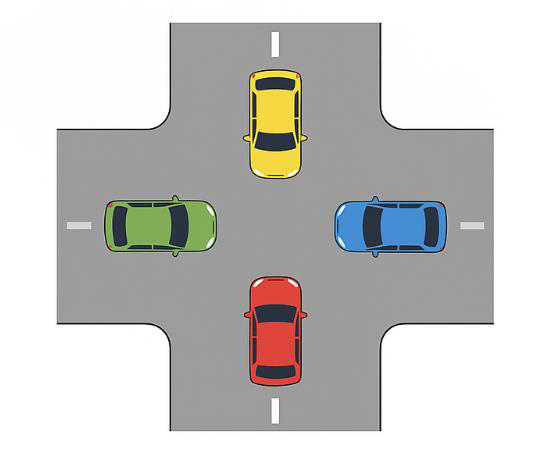
\includegraphics[width=0.55\linewidth,height=\textheight,keepaspectratio,alt={Cuatro vehículos bloqueados en una intersección}]{capitulos/img/interbloqueos/cruce_vehicular.png}

}

\caption{Cruce vehicular usado como analogía de un interbloqueo.}

\end{figure}%

\begin{tcolorbox}[enhanced jigsaw, arc=.35mm, bottomrule=.15mm, bottomtitle=1mm, breakable, colback=white, colbacktitle=quarto-callout-note-color!10!white, colframe=quarto-callout-note-color-frame, coltitle=black, left=2mm, leftrule=.75mm, opacityback=0, opacitybacktitle=0.6, rightrule=.15mm, title=\textcolor{quarto-callout-note-color}{\faInfo}\hspace{0.5em}{Pregunta detonadora}, titlerule=0mm, toprule=.15mm, toptitle=1mm]

Si todos los procesos están esperando, ¿quién será el primero en liberar
el recurso que los demás necesitan?

\end{tcolorbox}

Esta idea aparentemente sencilla nos permitirá comprender uno de los
problemas clásicos de los sistemas concurrentes.

\begin{center}\rule{0.5\linewidth}{0.5pt}\end{center}

\bookmarksetup{startatroot}

\chapter{¿Qué es un interbloqueo?}\label{quuxe9-es-un-interbloqueo}

Un \textbf{interbloqueo (deadlock)} ocurre cuando dos o más procesos
permanecen esperando indefinidamente por recursos que no pueden obtener
porque están retenidos por otros procesos que también se encuentran
esperando.

En otras palabras:

\begin{quote}
\textbf{Cada proceso espera algo que otro proceso posee, y ninguno puede
continuar.}
\end{quote}

El resultado es un \textbf{bloqueo mutuo}.

Los procesos involucrados no avanzan, aunque el sistema operativo
continúe funcionando.

\begin{center}\rule{0.5\linewidth}{0.5pt}\end{center}

\bookmarksetup{startatroot}

\chapter{Un ejemplo mínimo con dos
procesos}\label{un-ejemplo-muxednimo-con-dos-procesos}

Supongamos que existen:

\begin{itemize}
\tightlist
\item
  \textbf{Proceso P1}
\item
  \textbf{Proceso P2}
\item
  \textbf{Recurso R1}
\item
  \textbf{Recurso R2}
\end{itemize}

La secuencia es la siguiente:

\begin{enumerate}
\def\labelenumi{\arabic{enumi}.}
\tightlist
\item
  P1 obtiene R1.
\item
  P2 obtiene R2.
\item
  P1 solicita R2 y debe esperar.
\item
  P2 solicita R1 y también debe esperar.
\end{enumerate}

\begin{figure}[H]

{\centering 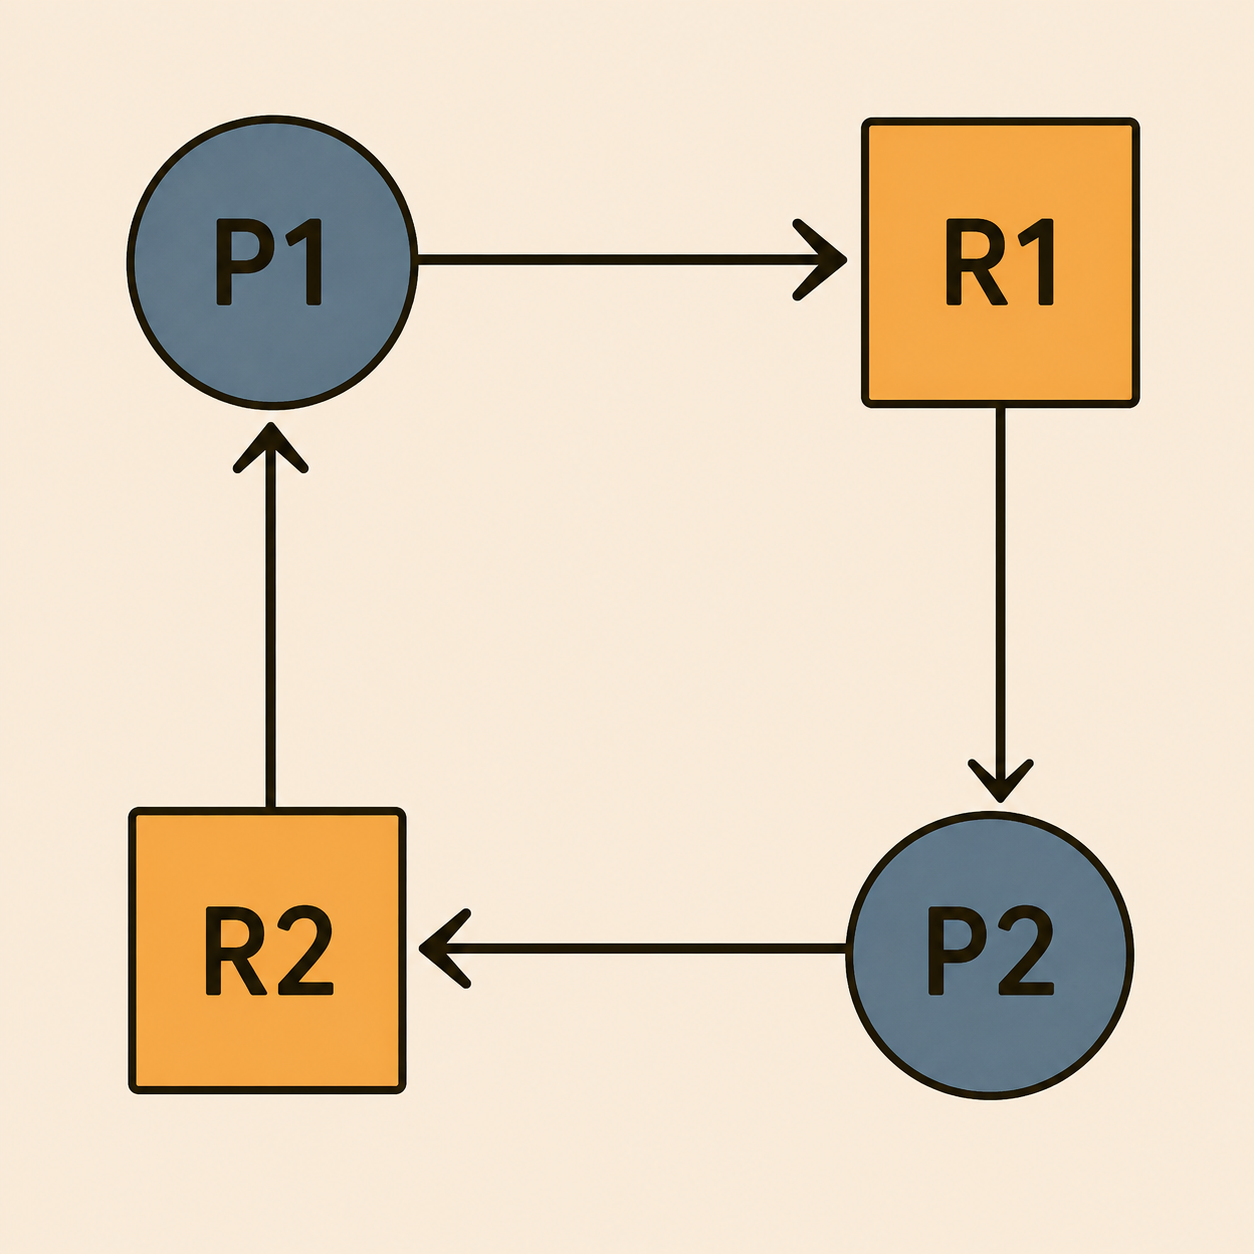
\includegraphics[width=0.58\linewidth,height=\textheight,keepaspectratio,alt={Diagrama de dos procesos y dos recursos en interbloqueo}]{capitulos/img/interbloqueos/interbloqueo_procesos.png}

}

\caption{Dos procesos reteniendo un recurso y esperando el recurso del
otro.}

\end{figure}%

Ninguno puede continuar.

\begin{Shaded}
\begin{Highlighting}[]
\NormalTok{P1 tiene R1 y espera R2}
\NormalTok{P2 tiene R2 y espera R1}
\end{Highlighting}
\end{Shaded}

\begin{tcolorbox}[enhanced jigsaw, arc=.35mm, bottomrule=.15mm, bottomtitle=1mm, breakable, colback=white, colbacktitle=quarto-callout-warning-color!10!white, colframe=quarto-callout-warning-color-frame, coltitle=black, left=2mm, leftrule=.75mm, opacityback=0, opacitybacktitle=0.6, rightrule=.15mm, title=\textcolor{quarto-callout-warning-color}{\faExclamationTriangle}\hspace{0.5em}{El problema}, titlerule=0mm, toprule=.15mm, toptitle=1mm]

P1 no libera R1 porque todavía necesita terminar.

P2 no libera R2 por la misma razón.

Ambos esperan indefinidamente.

\end{tcolorbox}

\begin{center}\rule{0.5\linewidth}{0.5pt}\end{center}

\bookmarksetup{startatroot}

\chapter{Las cuatro condiciones
necesarias}\label{las-cuatro-condiciones-necesarias}

Para que pueda existir un interbloqueo deben presentarse
\textbf{simultáneamente cuatro condiciones}.

\section{1. Exclusión mutua}\label{exclusiuxf3n-mutua}

Al menos un recurso debe estar disponible para \textbf{un solo proceso a
la vez}.

Ejemplos:

\begin{itemize}
\tightlist
\item
  Una impresora.
\item
  Un archivo abierto exclusivamente para escritura.
\item
  Un escáner.
\item
  Un bloqueo de base de datos.
\end{itemize}

Si un proceso está utilizando ese recurso, otro proceso debe esperar.

\begin{center}\rule{0.5\linewidth}{0.5pt}\end{center}

\bookmarksetup{startatroot}

\chapter{2. Retención y espera}\label{retenciuxf3n-y-espera}

Un proceso conserva uno o más recursos mientras espera obtener otros.

Ejemplo:

\begin{Shaded}
\begin{Highlighting}[]
\NormalTok{P1 tiene R1}
\NormalTok{P1 espera R2}
\end{Highlighting}
\end{Shaded}

P1 no libera R1 mientras intenta obtener R2.

Esta combinación de \textbf{tener} y \textbf{esperar} es fundamental
para que aparezca el problema.

\begin{center}\rule{0.5\linewidth}{0.5pt}\end{center}

\bookmarksetup{startatroot}

\chapter{3. No expropiación}\label{no-expropiaciuxf3n}

El Sistema Operativo no puede retirar arbitrariamente un recurso que ya
fue asignado a un proceso.

El proceso debe:

\begin{itemize}
\tightlist
\item
  utilizarlo,
\item
  terminar su operación,
\item
  y liberarlo voluntariamente.
\end{itemize}

\begin{tcolorbox}[enhanced jigsaw, arc=.35mm, bottomrule=.15mm, bottomtitle=1mm, breakable, colback=white, colbacktitle=quarto-callout-note-color!10!white, colframe=quarto-callout-note-color-frame, coltitle=black, left=2mm, leftrule=.75mm, opacityback=0, opacitybacktitle=0.6, rightrule=.15mm, title=\textcolor{quarto-callout-note-color}{\faInfo}\hspace{0.5em}{Ejemplo}, titlerule=0mm, toprule=.15mm, toptitle=1mm]

Si un proceso está escribiendo en un archivo, retirarle el recurso en
cualquier momento podría dejar la información inconsistente.

\end{tcolorbox}

\begin{center}\rule{0.5\linewidth}{0.5pt}\end{center}

\bookmarksetup{startatroot}

\chapter{4. Espera circular}\label{espera-circular}

Existe un ciclo en el cual cada proceso espera un recurso retenido por
el siguiente proceso.

Por ejemplo:

\begin{Shaded}
\begin{Highlighting}[]
\NormalTok{P1 espera un recurso de P2}
\NormalTok{P2 espera un recurso de P3}
\NormalTok{P3 espera un recurso de P1}
\end{Highlighting}
\end{Shaded}

En el caso más simple:

\begin{Shaded}
\begin{Highlighting}[]
\NormalTok{P1 espera R2}
\NormalTok{P2 espera R1}
\end{Highlighting}
\end{Shaded}

\begin{figure}[H]

{\centering 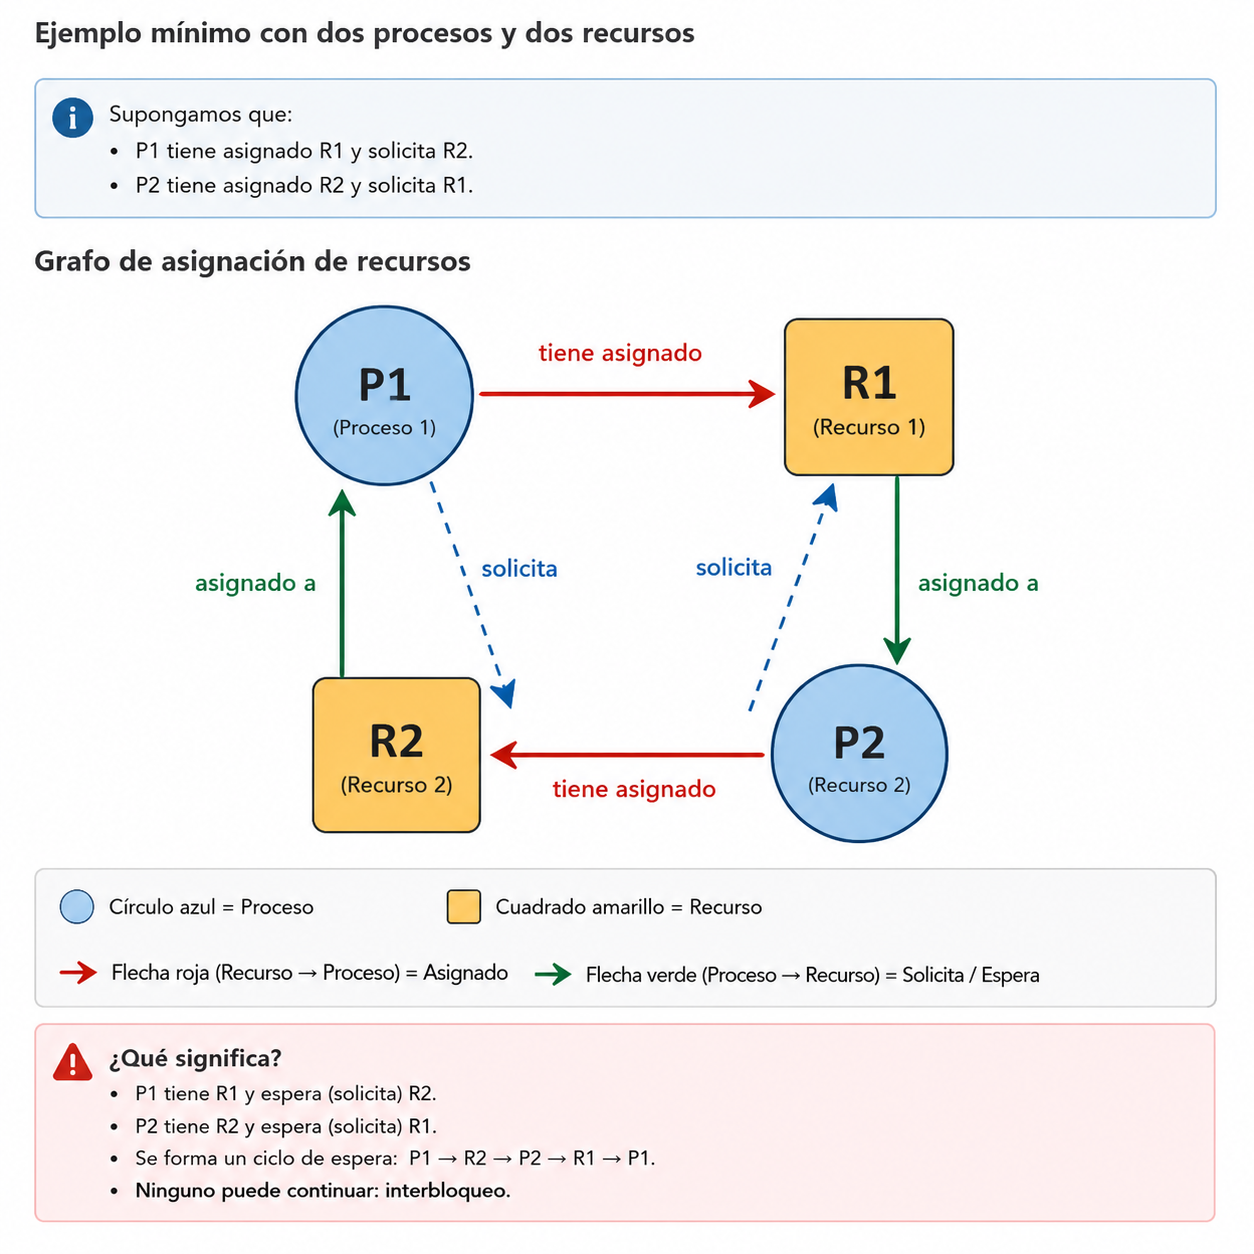
\includegraphics[width=0.58\linewidth,height=\textheight,keepaspectratio,alt={Ciclo de espera que representa un interbloqueo}]{capitulos/img/interbloqueos/ciclo_espera.png}

}

\caption{Representación del ciclo de espera entre procesos y recursos.}

\end{figure}%

La espera circular cierra el ciclo y evita que alguno de los procesos
pueda avanzar.

\begin{center}\rule{0.5\linewidth}{0.5pt}\end{center}

\bookmarksetup{startatroot}

\chapter{Idea clave: deben cumplirse las
cuatro}\label{idea-clave-deben-cumplirse-las-cuatro}

Un interbloqueo requiere que las cuatro condiciones existan al mismo
tiempo:

{\def\LTcaptype{none} % do not increment counter
\begin{longtable}[]{@{}
  >{\raggedright\arraybackslash}p{(\linewidth - 2\tabcolsep) * \real{0.5000}}
  >{\raggedright\arraybackslash}p{(\linewidth - 2\tabcolsep) * \real{0.5000}}@{}}
\toprule\noalign{}
\begin{minipage}[b]{\linewidth}\raggedright
Condición
\end{minipage} & \begin{minipage}[b]{\linewidth}\raggedright
Pregunta para identificarla
\end{minipage} \\
\midrule\noalign{}
\endhead
\bottomrule\noalign{}
\endlastfoot
Exclusión mutua & ¿Hay un recurso que solo puede usar un proceso a la
vez? \\
Retención y espera & ¿Algún proceso conserva un recurso mientras espera
otro? \\
No expropiación & ¿El recurso no puede retirarse por la fuerza? \\
Espera circular & ¿Existe un ciclo de procesos esperando recursos entre
sí? \\
\end{longtable}
}

\begin{tcolorbox}[enhanced jigsaw, arc=.35mm, bottomrule=.15mm, bottomtitle=1mm, breakable, colback=white, colbacktitle=quarto-callout-tip-color!10!white, colframe=quarto-callout-tip-color-frame, coltitle=black, left=2mm, leftrule=.75mm, opacityback=0, opacitybacktitle=0.6, rightrule=.15mm, title=\textcolor{quarto-callout-tip-color}{\faLightbulb}\hspace{0.5em}{Regla para recordar}, titlerule=0mm, toprule=.15mm, toptitle=1mm]

Si logramos eliminar \textbf{al menos una} de estas condiciones, el
interbloqueo no puede formarse de esa manera.

\end{tcolorbox}

\begin{center}\rule{0.5\linewidth}{0.5pt}\end{center}

\bookmarksetup{startatroot}

\chapter{Tipos de recursos}\label{tipos-de-recursos}

No todos los recursos se comportan igual.

\section{Recursos exclusivos}\label{recursos-exclusivos}

Solo un proceso puede utilizarlos en un momento determinado.

Ejemplos:

\begin{itemize}
\tightlist
\item
  Impresora.
\item
  Escáner.
\item
  Archivo con bloqueo exclusivo.
\item
  Sección crítica protegida por un mutex.
\end{itemize}

Estos recursos son especialmente importantes cuando estudiamos
interbloqueos.

\section{Recursos compartidos}\label{recursos-compartidos-1}

Pueden ser utilizados por varios procesos, dependiendo de las reglas de
acceso.

Ejemplos:

\begin{itemize}
\tightlist
\item
  Memoria compartida.
\item
  Datos de solo lectura.
\item
  Algunos recursos del sistema con acceso concurrente controlado.
\end{itemize}

\begin{tcolorbox}[enhanced jigsaw, arc=.35mm, bottomrule=.15mm, bottomtitle=1mm, breakable, colback=white, colbacktitle=quarto-callout-note-color!10!white, colframe=quarto-callout-note-color-frame, coltitle=black, left=2mm, leftrule=.75mm, opacityback=0, opacitybacktitle=0.6, rightrule=.15mm, title=\textcolor{quarto-callout-note-color}{\faInfo}\hspace{0.5em}{Importante}, titlerule=0mm, toprule=.15mm, toptitle=1mm]

Los interbloqueos aparecen con mayor frecuencia cuando existen
\textbf{recursos de uso exclusivo} y varios procesos compiten por ellos.

\end{tcolorbox}

\begin{center}\rule{0.5\linewidth}{0.5pt}\end{center}

\bookmarksetup{startatroot}

\chapter{¿Qué componentes del Sistema Operativo están
implicados?}\label{quuxe9-componentes-del-sistema-operativo-estuxe1n-implicados}

Los interbloqueos aparecen dentro del mismo entorno que hemos venido
estudiando.

Participan principalmente:

\begin{itemize}
\tightlist
\item
  \textbf{Procesos o hilos}, que solicitan recursos.
\item
  \textbf{Gestor de recursos}, que administra memoria, archivos y
  dispositivos.
\item
  \textbf{Kernel}, que coordina la asignación y liberación.
\item
  \textbf{Mecanismos de sincronización}, como semáforos y mutex.
\item
  \textbf{Dispositivos y recursos de E/S}, que pueden estar ocupados por
  un proceso.
\end{itemize}

Esto conecta directamente los interbloqueos con los temas de:

\begin{itemize}
\tightlist
\item
  procesos,
\item
  concurrencia,
\item
  sincronización,
\item
  administración de recursos.
\end{itemize}

\begin{center}\rule{0.5\linewidth}{0.5pt}\end{center}

\bookmarksetup{startatroot}

\chapter{Ejemplo real: cruce
vehicular}\label{ejemplo-real-cruce-vehicular}

Regresemos al ejemplo de la intersección.

\begin{figure}[H]

{\centering 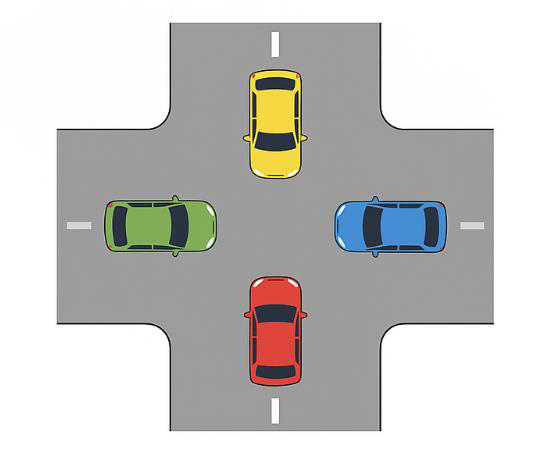
\includegraphics[width=0.5\linewidth,height=\textheight,keepaspectratio,alt={Cruce vehicular con cuatro automóviles bloqueados}]{capitulos/img/interbloqueos/cruce_vehicular.png}

}

\caption{Cruce de cuatro vehículos usado para representar un ciclo de
espera.}

\end{figure}%

Podemos hacer la siguiente analogía:

{\def\LTcaptype{none} % do not increment counter
\begin{longtable}[]{@{}ll@{}}
\toprule\noalign{}
Situación real & Sistema Operativo \\
\midrule\noalign{}
\endhead
\bottomrule\noalign{}
\endlastfoot
Cada vehículo & Un proceso \\
Espacio de la intersección & Un recurso \\
Vehículo esperando avanzar & Proceso esperando un recurso \\
Ningún vehículo se mueve & Ningún proceso avanza \\
\end{longtable}
}

Cada vehículo ocupa una parte de la intersección y necesita el siguiente
espacio para continuar.

Se forma un ciclo:

\begin{Shaded}
\begin{Highlighting}[]
\NormalTok{Auto A espera a B}
\NormalTok{Auto B espera a C}
\NormalTok{Auto C espera a D}
\NormalTok{Auto D espera a A}
\end{Highlighting}
\end{Shaded}

Eso es exactamente una \textbf{espera circular}.

\begin{center}\rule{0.5\linewidth}{0.5pt}\end{center}

\bookmarksetup{startatroot}

\chapter{Ejemplo clásico: filósofos
comensales}\label{ejemplo-cluxe1sico-filuxf3sofos-comensales}

Cinco filósofos se sientan alrededor de una mesa.

Entre cada par de filósofos existe un tenedor.

Para comer, cada filósofo necesita \textbf{dos tenedores}:

\begin{itemize}
\tightlist
\item
  uno a la izquierda,
\item
  uno a la derecha.
\end{itemize}

\begin{figure}[H]

{\centering 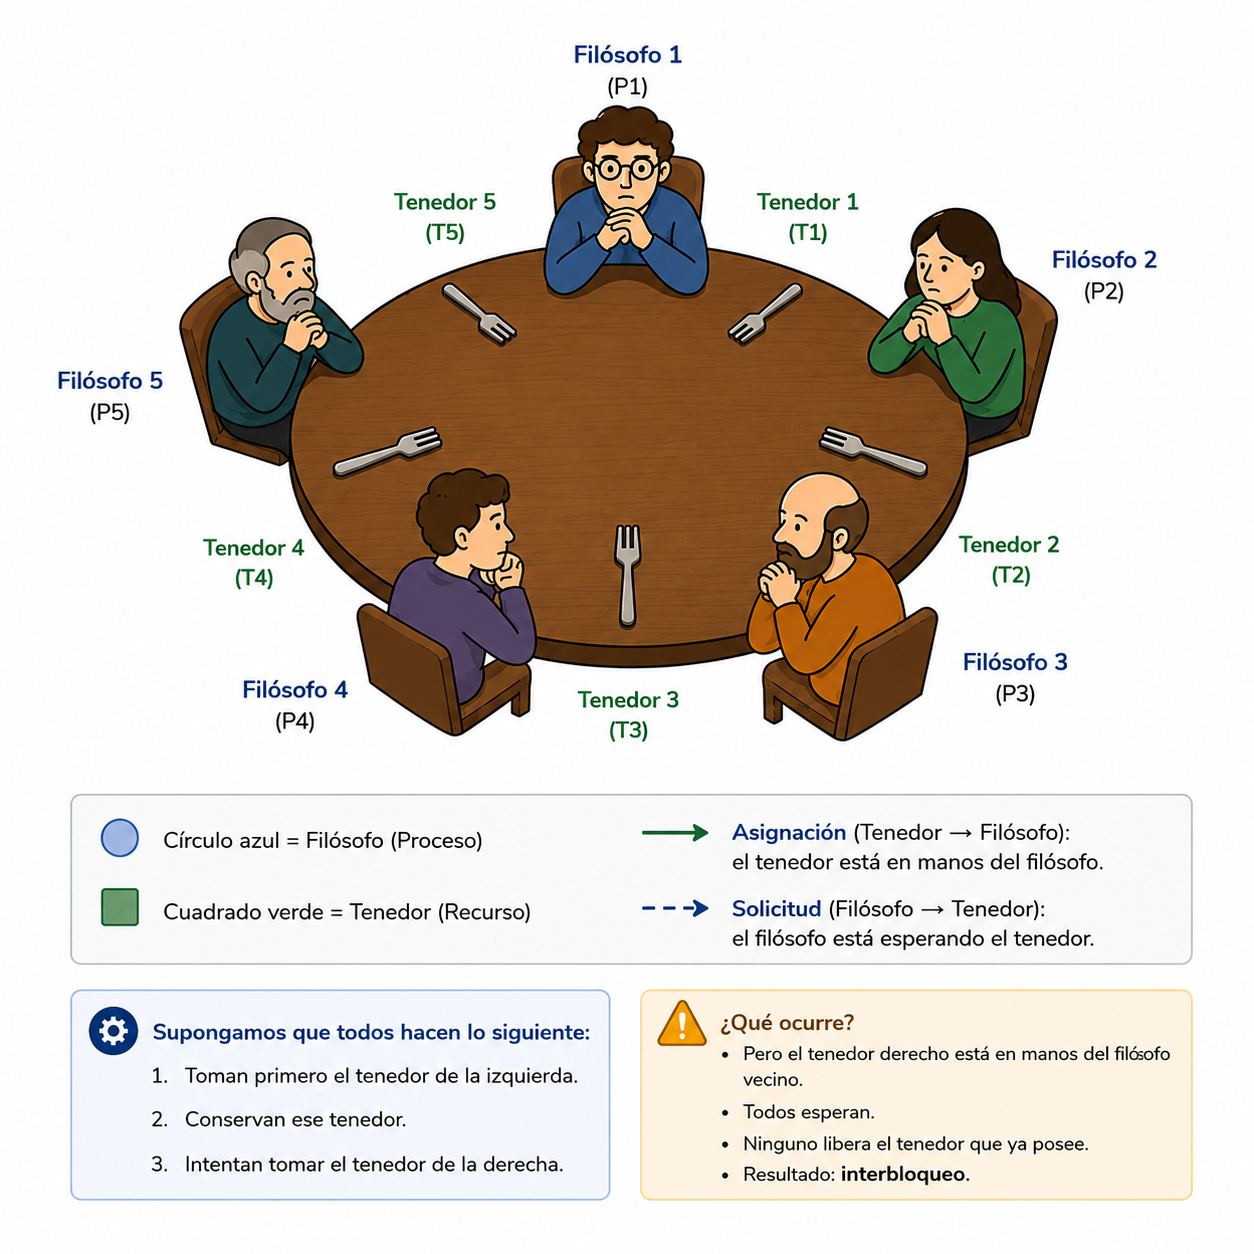
\includegraphics[width=0.82\linewidth,height=\textheight,keepaspectratio,alt={Cinco filósofos sentados alrededor de una mesa con tenedores}]{capitulos/img/interbloqueos/filosofos_comensales.png}

}

\caption{Problema clásico de los filósofos comensales.}

\end{figure}%

\begin{center}\rule{0.5\linewidth}{0.5pt}\end{center}

\bookmarksetup{startatroot}

\chapter{Analizando a los filósofos con las cuatro
condiciones}\label{analizando-a-los-filuxf3sofos-con-las-cuatro-condiciones}

{\def\LTcaptype{none} % do not increment counter
\begin{longtable}[]{@{}
  >{\raggedright\arraybackslash}p{(\linewidth - 2\tabcolsep) * \real{0.5000}}
  >{\raggedright\arraybackslash}p{(\linewidth - 2\tabcolsep) * \real{0.5000}}@{}}
\toprule\noalign{}
\begin{minipage}[b]{\linewidth}\raggedright
Condición
\end{minipage} & \begin{minipage}[b]{\linewidth}\raggedright
¿Cómo aparece?
\end{minipage} \\
\midrule\noalign{}
\endhead
\bottomrule\noalign{}
\endlastfoot
Exclusión mutua & Cada tenedor solo puede estar en manos de un
filósofo \\
Retención y espera & Cada filósofo conserva un tenedor y espera otro \\
No expropiación & No se le quita el tenedor por la fuerza \\
Espera circular & Cada filósofo espera el tenedor del vecino \\
\end{longtable}
}

El ejemplo es útil porque permite visualizar las cuatro condiciones en
una sola situación.

\begin{center}\rule{0.5\linewidth}{0.5pt}\end{center}

\bookmarksetup{startatroot}

\chapter{Ejemplo adicional: impresoras en
red}\label{ejemplo-adicional-impresoras-en-red}

Dos usuarios necesitan utilizar:

\begin{itemize}
\tightlist
\item
  una impresora,
\item
  y un conjunto de archivos compartidos.
\end{itemize}

\begin{figure}[H]

{\centering 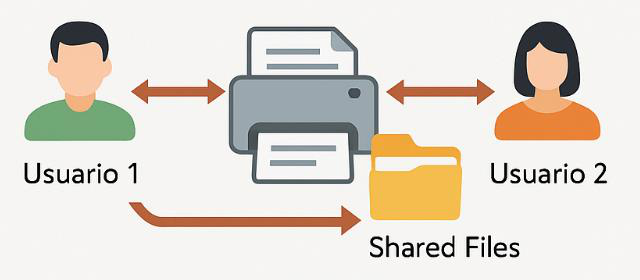
\includegraphics[width=0.58\linewidth,height=\textheight,keepaspectratio,alt={Usuarios, impresora y archivos compartidos}]{capitulos/img/interbloqueos/impresoras_red.png}

}

\caption{Dos usuarios compitiendo por una impresora y archivos
compartidos.}

\end{figure}%

Supongamos que ocurre lo siguiente:

\begin{itemize}
\tightlist
\item
  Usuario 1 obtiene la impresora y espera los archivos.
\item
  Usuario 2 obtiene los archivos y espera la impresora.
\end{itemize}

Entonces:

\begin{Shaded}
\begin{Highlighting}[]
\NormalTok{Usuario 1 → espera archivos}
\NormalTok{Usuario 2 → espera impresora}
\end{Highlighting}
\end{Shaded}

Se forma un ciclo de espera mutua.

\section{¿Cómo podría evitarse?}\label{cuxf3mo-podruxeda-evitarse}

Dos ideas sencillas son:

\begin{itemize}
\tightlist
\item
  establecer un orden obligatorio para solicitar recursos,
\item
  liberar un recurso antes de solicitar otro.
\end{itemize}

\begin{center}\rule{0.5\linewidth}{0.5pt}\end{center}

\bookmarksetup{startatroot}

\chapter{Ejemplo adicional: software de
oficina}\label{ejemplo-adicional-software-de-oficina}

Dos aplicaciones intentan trabajar con recursos que necesitan
simultáneamente.

Por ejemplo:

\begin{itemize}
\tightlist
\item
  Aplicación A tiene bloqueado un archivo y espera memoria.
\item
  Aplicación B tiene reservada memoria y espera el archivo.
\end{itemize}

La situación puede representarse así:

\begin{Shaded}
\begin{Highlighting}[]
\NormalTok{Aplicación A: tiene Archivo → espera Memoria}
\NormalTok{Aplicación B: tiene Memoria → espera Archivo}
\end{Highlighting}
\end{Shaded}

De nuevo aparece la espera circular.

\begin{tcolorbox}[enhanced jigsaw, arc=.35mm, bottomrule=.15mm, bottomtitle=1mm, breakable, colback=white, colbacktitle=quarto-callout-tip-color!10!white, colframe=quarto-callout-tip-color-frame, coltitle=black, left=2mm, leftrule=.75mm, opacityback=0, opacitybacktitle=0.6, rightrule=.15mm, title=\textcolor{quarto-callout-tip-color}{\faLightbulb}\hspace{0.5em}{Pregunta para analizar}, titlerule=0mm, toprule=.15mm, toptitle=1mm]

¿Cuáles de las cuatro condiciones puedes identificar en este escenario?

\end{tcolorbox}

\begin{center}\rule{0.5\linewidth}{0.5pt}\end{center}

\bookmarksetup{startatroot}

\chapter{Ejemplo adicional: cajero
automático}\label{ejemplo-adicional-cajero-automuxe1tico}

Un cajero automático necesita comunicarse con varios recursos mientras
procesa una transacción.

Entre ellos:

\begin{itemize}
\tightlist
\item
  conexión con el cliente,
\item
  base de datos bancaria,
\item
  sistema de autorización,
\item
  dispositivo dispensador.
\end{itemize}

\begin{figure}[H]

{\centering 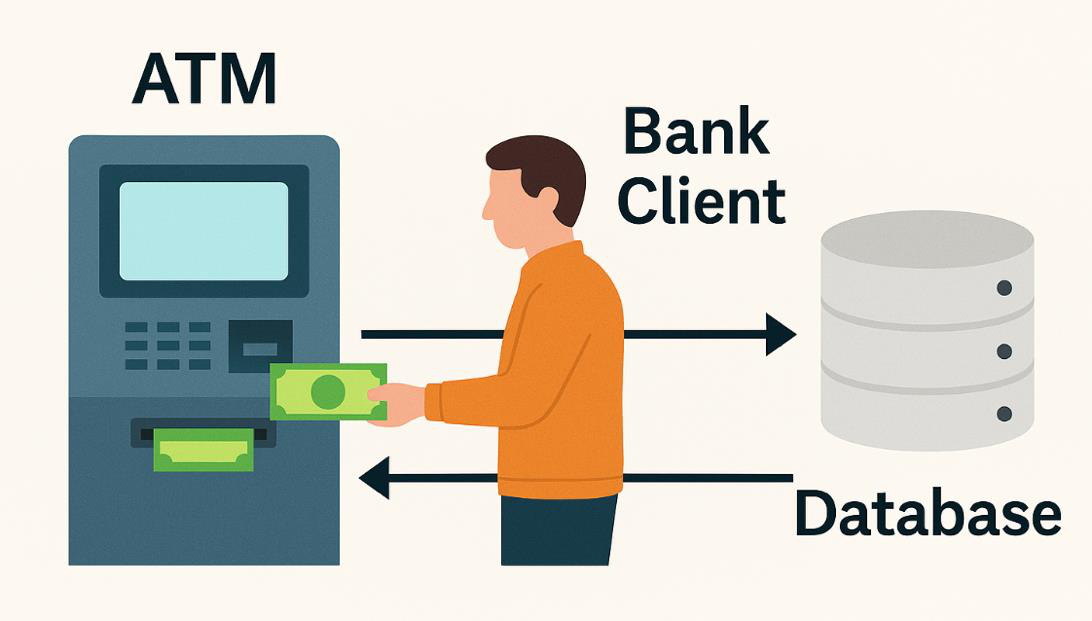
\includegraphics[width=0.6\linewidth,height=\textheight,keepaspectratio,alt={Cajero automático conectado a una base de datos}]{capitulos/img/interbloqueos/cajero_atm.png}

}

\caption{Ejemplo conceptual de un ATM comunicándose con una base de
datos bancaria.}

\end{figure}%

Si una operación retiene un recurso y espera otro que está bloqueado por
una segunda operación, puede formarse una espera mutua.

Una estrategia mencionada en el material es:

\begin{itemize}
\tightlist
\item
  liberar recursos cuando una transacción falla,
\item
  o utilizar temporizadores para evitar esperas indefinidas.
\end{itemize}

\begin{center}\rule{0.5\linewidth}{0.5pt}\end{center}

\bookmarksetup{startatroot}

\chapter{Actividad en clase: identifiquemos el
interbloqueo}\label{actividad-en-clase-identifiquemos-el-interbloqueo}

Formen grupos y analicen el siguiente escenario:

\begin{quote}
\textbf{Proceso A tiene la impresora y solicita acceso a la base de
datos.\\
Proceso B tiene la base de datos y solicita la impresora.}
\end{quote}

Respondan:

\begin{enumerate}
\def\labelenumi{\arabic{enumi}.}
\tightlist
\item
  ¿Qué recurso tiene el Proceso A?
\item
  ¿Qué recurso espera?
\item
  ¿Qué recurso tiene el Proceso B?
\item
  ¿Qué recurso espera?
\item
  ¿Se cumplen las cuatro condiciones de interbloqueo?
\item
  Dibujen el ciclo de espera.
\end{enumerate}

\begin{center}\rule{0.5\linewidth}{0.5pt}\end{center}

\bookmarksetup{startatroot}

\chapter{Actividades por grupos}\label{actividades-por-grupos}

\section{Grupo 1. Cruce vehicular}\label{grupo-1.-cruce-vehicular}

Dibujen una intersección con cuatro autos sin semáforo.

Identifiquen:

\begin{itemize}
\tightlist
\item
  Qué recurso tiene cada auto.
\item
  Qué recurso espera.
\item
  Dónde está la espera circular.
\end{itemize}

\section{Grupo 2. Filósofos
comensales}\label{grupo-2.-filuxf3sofos-comensales}

Analicen el problema clásico.

Respondan:

\begin{enumerate}
\def\labelenumi{\arabic{enumi}.}
\tightlist
\item
  ¿Qué representa cada filósofo?
\item
  ¿Qué representan los tenedores?
\item
  ¿Cómo podría evitarse el interbloqueo?
\end{enumerate}

\section{Grupo 3. Las cuatro
condiciones}\label{grupo-3.-las-cuatro-condiciones}

Utilicen el escenario de la impresora y la base de datos.

Identifiquen:

\begin{enumerate}
\def\labelenumi{\arabic{enumi}.}
\tightlist
\item
  Exclusión mutua.
\item
  Retención y espera.
\item
  No expropiación.
\item
  Espera circular.
\end{enumerate}

\section{Grupo 4. Clasificación de
recursos}\label{grupo-4.-clasificaciuxf3n-de-recursos}

Clasifiquen como \textbf{exclusivos} o \textbf{compartidos}:

\begin{itemize}
\tightlist
\item
  Impresora.
\item
  Archivo.
\item
  CPU.
\item
  Memoria compartida.
\item
  Escáner.
\item
  Variables globales.
\end{itemize}

\section{Grupo 5. Una historia de
interbloqueo}\label{grupo-5.-una-historia-de-interbloqueo}

Inventen una historia con:

\begin{itemize}
\tightlist
\item
  2 personas,
\item
  2 recursos,
\item
  una situación de bloqueo mutuo.
\end{itemize}

Luego indiquen:

\begin{itemize}
\tightlist
\item
  quiénes representan los procesos,
\item
  cuáles son los recursos,
\item
  y cómo podría evitarse.
\end{itemize}

\section{Grupo 6. Semáforo lógico}\label{grupo-6.-semuxe1foro-luxf3gico}

Simulen cómo un \textbf{semáforo} o un \textbf{árbitro} podría evitar:

\begin{itemize}
\tightlist
\item
  el interbloqueo del cruce,
\item
  o el interbloqueo de los filósofos.
\end{itemize}

Respondan:

\begin{quote}
¿Qué condición deja de cumplirse cuando existe ese mecanismo de control?
\end{quote}

\begin{center}\rule{0.5\linewidth}{0.5pt}\end{center}

\bookmarksetup{startatroot}

\chapter{Soluciones para discusión}\label{soluciones-para-discusiuxf3n}

Esta sección puede utilizarse después de que los grupos presenten sus
respuestas.

\section{Grupo 1}\label{grupo-1}

Cada automóvil ocupa un espacio y espera el siguiente.

Se forma un ciclo:

\begin{Shaded}
\begin{Highlighting}[]
\NormalTok{A → B → C → D → A}
\end{Highlighting}
\end{Shaded}

\section{Grupo 2}\label{grupo-2}

\begin{itemize}
\tightlist
\item
  Filósofos → procesos.
\item
  Tenedores → recursos exclusivos.
\item
  Posibles soluciones: tomar ambos tenedores a la vez, limitar cuántos
  intentan comer o utilizar un árbitro.
\end{itemize}

\section{Grupo 3}\label{grupo-3}

Se cumplen:

\begin{enumerate}
\def\labelenumi{\arabic{enumi}.}
\tightlist
\item
  Exclusión mutua.
\item
  Retención y espera.
\item
  No expropiación.
\item
  Espera circular.
\end{enumerate}

\section{Grupo 4}\label{grupo-4}

De acuerdo con la clasificación planteada en el material de clase:

\begin{itemize}
\tightlist
\item
  \textbf{Exclusivos:} impresora, archivo, CPU, escáner.
\item
  \textbf{Compartidos:} memoria compartida, variables globales.
\end{itemize}

\section{Grupo 5}\label{grupo-5}

Ejemplo del material:

\begin{quote}
Ana utiliza el microondas y espera el cuchillo. Carlos tiene el cuchillo
y espera el microondas.
\end{quote}

Una forma de evitarlo es liberar un recurso antes de solicitar otro o
imponer un orden de solicitud.

\section{Grupo 6}\label{grupo-6}

El semáforo o árbitro controla el acceso y evita que todos entren
simultáneamente en una situación de espera circular.

\begin{center}\rule{0.5\linewidth}{0.5pt}\end{center}

\bookmarksetup{startatroot}

\chapter{¿Cómo evitar un
interbloqueo?}\label{cuxf3mo-evitar-un-interbloqueo}

En esta clase no estudiaremos todavía los algoritmos formales de
prevención y detección.

Sin embargo, los ejemplos ya nos permiten anticipar varias ideas:

\begin{itemize}
\tightlist
\item
  Solicitar recursos en un orden definido.
\item
  Evitar conservar recursos mientras se esperan otros.
\item
  Limitar cuántos procesos compiten al mismo tiempo.
\item
  Liberar recursos cuando una operación falla.
\item
  Utilizar un árbitro o mecanismo de coordinación.
\item
  Establecer tiempos máximos de espera en determinados escenarios.
\end{itemize}

\begin{tcolorbox}[enhanced jigsaw, arc=.35mm, bottomrule=.15mm, bottomtitle=1mm, breakable, colback=white, colbacktitle=quarto-callout-warning-color!10!white, colframe=quarto-callout-warning-color-frame, coltitle=black, left=2mm, leftrule=.75mm, opacityback=0, opacitybacktitle=0.6, rightrule=.15mm, title=\textcolor{quarto-callout-warning-color}{\faExclamationTriangle}\hspace{0.5em}{Importante}, titlerule=0mm, toprule=.15mm, toptitle=1mm]

Estas ideas introducen el siguiente tema.

En el próximo capítulo estudiaremos estrategias formales para
\textbf{prevenir, evitar, detectar y recuperar} interbloqueos.

\end{tcolorbox}

\begin{center}\rule{0.5\linewidth}{0.5pt}\end{center}

\bookmarksetup{startatroot}

\chapter{Caso integrador}\label{caso-integrador-1}

Supongamos que un sistema tiene dos procesos:

\begin{Shaded}
\begin{Highlighting}[]
\NormalTok{P1 necesita: Impresora + Archivo}
\NormalTok{P2 necesita: Archivo + Impresora}
\end{Highlighting}
\end{Shaded}

La ejecución ocurre así:

\begin{Shaded}
\begin{Highlighting}[]
\NormalTok{1. P1 obtiene la impresora.}
\NormalTok{2. P2 obtiene el archivo.}
\NormalTok{3. P1 solicita el archivo.}
\NormalTok{4. P2 solicita la impresora.}
\end{Highlighting}
\end{Shaded}

Analicemos:

{\def\LTcaptype{none} % do not increment counter
\begin{longtable}[]{@{}ll@{}}
\toprule\noalign{}
Pregunta & Respuesta \\
\midrule\noalign{}
\endhead
\bottomrule\noalign{}
\endlastfoot
¿P1 puede continuar? & No \\
¿P2 puede continuar? & No \\
¿P1 libera la impresora? & No mientras espera terminar \\
¿P2 libera el archivo? & No mientras espera terminar \\
¿Existe espera circular? & Sí \\
¿Existe interbloqueo? & Sí \\
\end{longtable}
}

Este pequeño ejemplo contiene la esencia del problema completo.

\begin{center}\rule{0.5\linewidth}{0.5pt}\end{center}

\bookmarksetup{startatroot}

\chapter{Autoevaluación}\label{autoevaluaciuxf3n-5}

\begin{enumerate}
\def\labelenumi{\arabic{enumi}.}
\tightlist
\item
  ¿Qué es un interbloqueo?
\item
  ¿Qué diferencia existe entre un proceso bloqueado temporalmente y un
  proceso en interbloqueo?
\item
  ¿Cuáles son las cuatro condiciones necesarias?
\item
  Explica con tus palabras la exclusión mutua.
\item
  ¿Qué significa retención y espera?
\item
  ¿Por qué la no expropiación favorece un interbloqueo?
\item
  ¿Qué representa la espera circular?
\item
  ¿Por qué el cruce vehicular es una buena analogía?
\item
  En los filósofos comensales, ¿qué representan los filósofos y los
  tenedores?
\item
  ¿Qué relación existe entre los interbloqueos y la administración de
  recursos del Kernel?
\item
  Construye un ejemplo con dos procesos y dos recursos.
\item
  Propón una forma sencilla de romper una de las cuatro condiciones.
\end{enumerate}

\begin{center}\rule{0.5\linewidth}{0.5pt}\end{center}

\bookmarksetup{startatroot}

\chapter{Resumen del capítulo}\label{resumen-del-capuxedtulo-2}

Durante este capítulo aprendimos que un \textbf{interbloqueo} ocurre
cuando varios procesos quedan esperando recursos retenidos entre sí y
ninguno puede avanzar.

Para que aparezca deben coincidir cuatro condiciones:

\begin{enumerate}
\def\labelenumi{\arabic{enumi}.}
\tightlist
\item
  \textbf{Exclusión mutua.}
\item
  \textbf{Retención y espera.}
\item
  \textbf{No expropiación.}
\item
  \textbf{Espera circular.}
\end{enumerate}

También analizamos ejemplos como:

\begin{itemize}
\tightlist
\item
  cruce vehicular,
\item
  filósofos comensales,
\item
  impresoras en red,
\item
  aplicaciones de oficina,
\item
  cajeros automáticos.
\end{itemize}

\begin{tcolorbox}[enhanced jigsaw, arc=.35mm, bottomrule=.15mm, bottomtitle=1mm, breakable, colback=white, colbacktitle=quarto-callout-note-color!10!white, colframe=quarto-callout-note-color-frame, coltitle=black, left=2mm, leftrule=.75mm, opacityback=0, opacitybacktitle=0.6, rightrule=.15mm, title=\textcolor{quarto-callout-note-color}{\faInfo}\hspace{0.5em}{Para recordar}, titlerule=0mm, toprule=.15mm, toptitle=1mm]

Un proceso esperando no implica necesariamente un interbloqueo.

El problema aparece cuando existe una \textbf{dependencia mutua que
impide el avance de todos los procesos involucrados}.

\end{tcolorbox}

\begin{center}\rule{0.5\linewidth}{0.5pt}\end{center}

\bookmarksetup{startatroot}

\chapter{Conexión con el siguiente
capítulo}\label{conexiuxf3n-con-el-siguiente-capuxedtulo-2}

Ya sabemos reconocer \textbf{cuándo} existe un interbloqueo y
\textbf{qué condiciones} permiten que ocurra.

La siguiente pregunta será:

\begin{quote}
\textbf{¿Qué puede hacer el Sistema Operativo para impedirlo o
resolverlo?}
\end{quote}

En el siguiente capítulo estudiaremos:

\begin{itemize}
\tightlist
\item
  Prevención de interbloqueos.
\item
  Evitación.
\item
  Detección.
\item
  Recuperación.
\item
  Algoritmos utilizados para analizar estados seguros e inseguros.
\end{itemize}

\begin{center}\rule{0.5\linewidth}{0.5pt}\end{center}

\bookmarksetup{startatroot}

\chapter{Bibliografía base}\label{bibliografuxeda-base}

El material de clase propone como referencias:

\begin{itemize}
\tightlist
\item
  Tanenbaum, capítulo 7.1.
\item
  Deitel, capítulo 5.1.
\end{itemize}

\bookmarksetup{startatroot}

\chapter{Capítulo 9. Prevención, detección y recuperación de
interbloqueos}\label{capuxedtulo-9.-prevenciuxf3n-detecciuxf3n-y-recuperaciuxf3n-de-interbloqueos}

\section{Relación con la clase
anterior}\label{relaciuxf3n-con-la-clase-anterior-3}

En el capítulo anterior aprendimos a reconocer un \textbf{interbloqueo
(deadlock)} y estudiamos las cuatro condiciones necesarias para que
pueda aparecer:

\begin{enumerate}
\def\labelenumi{\arabic{enumi}.}
\tightlist
\item
  Exclusión mutua.
\item
  Retención y espera.
\item
  No expropiación.
\item
  Espera circular.
\end{enumerate}

También analizamos casos con procesos que conservan recursos mientras
esperan otros. Ahora damos el siguiente paso:

\begin{quote}
\textbf{Si ya sabemos cómo se forma un interbloqueo, ¿qué puede hacer el
Sistema Operativo para impedirlo, detectarlo o recuperarse cuando ya
ocurrió?}
\end{quote}

\begin{center}\rule{0.5\linewidth}{0.5pt}\end{center}

\bookmarksetup{startatroot}

\chapter{Objetivos de aprendizaje}\label{objetivos-de-aprendizaje-7}

Al finalizar este capítulo serás capaz de:

\begin{itemize}
\tightlist
\item
  Explicar cómo se \textbf{previenen} interbloqueos rompiendo al menos
  una condición necesaria.
\item
  Analizar las ventajas y desventajas de distintas políticas de
  prevención.
\item
  Interpretar un \textbf{grafo de asignación de recursos} para
  identificar ciclos de espera.
\item
  Diferenciar \textbf{prevención, evitación, detección y recuperación}.
\item
  Comprender la idea de \textbf{estado seguro} y la lógica general del
  algoritmo del banquero.
\item
  Proponer una estrategia de recuperación ante un interbloqueo sencillo.
\end{itemize}

\begin{center}\rule{0.5\linewidth}{0.5pt}\end{center}

\bookmarksetup{startatroot}

\chapter{1. Recordemos antes de
avanzar}\label{recordemos-antes-de-avanzar}

\begin{tcolorbox}[enhanced jigsaw, arc=.35mm, bottomrule=.15mm, bottomtitle=1mm, breakable, colback=white, colbacktitle=quarto-callout-note-color!10!white, colframe=quarto-callout-note-color-frame, coltitle=black, left=2mm, leftrule=.75mm, opacityback=0, opacitybacktitle=0.6, rightrule=.15mm, title=\textcolor{quarto-callout-note-color}{\faInfo}\hspace{0.5em}{Pregunta para el grupo}, titlerule=0mm, toprule=.15mm, toptitle=1mm]

Sin consultar el capítulo anterior:

\textbf{¿Cuáles son las cuatro condiciones que deben cumplirse
simultáneamente para que exista un interbloqueo?}

\end{tcolorbox}

{\def\LTcaptype{none} % do not increment counter
\begin{longtable}[]{@{}
  >{\raggedright\arraybackslash}p{(\linewidth - 2\tabcolsep) * \real{0.5000}}
  >{\raggedright\arraybackslash}p{(\linewidth - 2\tabcolsep) * \real{0.5000}}@{}}
\toprule\noalign{}
\begin{minipage}[b]{\linewidth}\raggedright
Condición
\end{minipage} & \begin{minipage}[b]{\linewidth}\raggedright
Idea principal
\end{minipage} \\
\midrule\noalign{}
\endhead
\bottomrule\noalign{}
\endlastfoot
Exclusión mutua & Un recurso solo puede ser utilizado por un proceso a
la vez \\
Retención y espera & Un proceso conserva recursos mientras solicita
otros \\
No expropiación & Un recurso no puede retirarse arbitrariamente \\
Espera circular & Existe un ciclo de procesos esperando recursos entre
sí \\
\end{longtable}
}

La idea central de la \textbf{prevención} es sencilla:

\begin{quote}
Si evitamos que al menos una de estas condiciones pueda cumplirse,
rompemos la posibilidad de formar ese interbloqueo.
\end{quote}

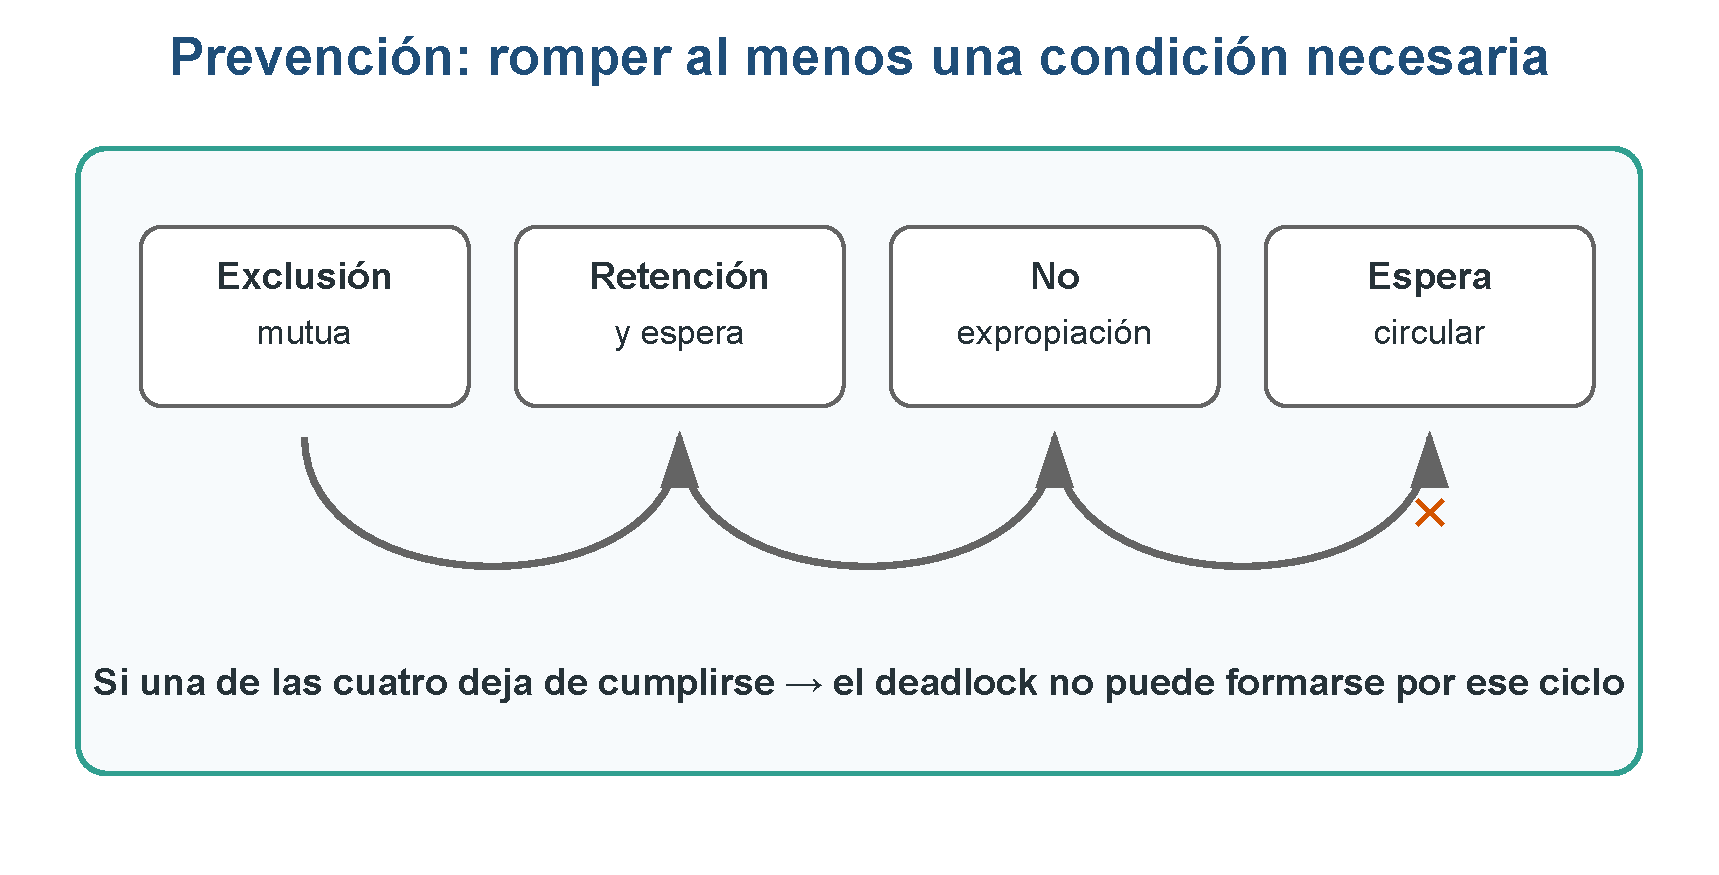
\includegraphics[width=0.92\linewidth,height=\textheight,keepaspectratio]{index_files/mediabag/capitulos/img/prevencion_interbloqueos/romper_condicion.pdf}

\begin{center}\rule{0.5\linewidth}{0.5pt}\end{center}

\bookmarksetup{startatroot}

\chapter{2. ¿Por qué prevenir
interbloqueos?}\label{por-quuxe9-prevenir-interbloqueos}

Un interbloqueo puede provocar que procesos permanezcan detenidos
indefinidamente.

Algunos efectos posibles son:

\begin{itemize}
\tightlist
\item
  documentos que nunca llegan a imprimirse;
\item
  transacciones que no pueden continuar;
\item
  recursos ocupados sin realizar trabajo útil;
\item
  usuarios esperando operaciones que no terminan;
\item
  pérdida de rendimiento y disponibilidad.
\end{itemize}

En sistemas críticos ---por ejemplo, bancos, hospitales o sistemas de
control--- el comportamiento debe ser especialmente predecible.

\begin{tcolorbox}[enhanced jigsaw, arc=.35mm, bottomrule=.15mm, bottomtitle=1mm, breakable, colback=white, colbacktitle=quarto-callout-important-color!10!white, colframe=quarto-callout-important-color-frame, coltitle=black, left=2mm, leftrule=.75mm, opacityback=0, opacitybacktitle=0.6, rightrule=.15mm, title=\textcolor{quarto-callout-important-color}{\faExclamation}\hspace{0.5em}{Pensemos}, titlerule=0mm, toprule=.15mm, toptitle=1mm]

¿Siempre conviene prevenir un interbloqueo a cualquier costo?

Una política muy restrictiva puede evitar deadlocks, pero también puede
dejar recursos sin utilizar durante mucho tiempo.

\end{tcolorbox}

\begin{center}\rule{0.5\linewidth}{0.5pt}\end{center}

\bookmarksetup{startatroot}

\chapter{3. Prevención: atacar las condiciones
necesarias}\label{prevenciuxf3n-atacar-las-condiciones-necesarias}

\section{3.1 Exclusión mutua}\label{exclusiuxf3n-mutua-1}

La exclusión mutua existe cuando un recurso no puede compartirse
simultáneamente.

Una estrategia consiste en \textbf{hacer compartibles los recursos
siempre que sea posible}.

Ejemplo:

\begin{itemize}
\tightlist
\item
  varios procesos pueden leer simultáneamente un archivo de solo
  lectura;
\item
  pero no siempre es posible compartir una impresora durante la
  impresión física de un documento.
\end{itemize}

\begin{tcolorbox}[enhanced jigsaw, arc=.35mm, bottomrule=.15mm, bottomtitle=1mm, breakable, colback=white, colbacktitle=quarto-callout-warning-color!10!white, colframe=quarto-callout-warning-color-frame, coltitle=black, left=2mm, leftrule=.75mm, opacityback=0, opacitybacktitle=0.6, rightrule=.15mm, title=\textcolor{quarto-callout-warning-color}{\faExclamationTriangle}\hspace{0.5em}{Limitación}, titlerule=0mm, toprule=.15mm, toptitle=1mm]

No podemos eliminar la exclusión mutua de todos los recursos. Algunos
son inherentemente exclusivos.

\end{tcolorbox}

\subsection{Mini ejercicio}\label{mini-ejercicio}

Clasifica estos recursos como \textbf{potencialmente compartibles} o
\textbf{normalmente exclusivos}:

\begin{enumerate}
\def\labelenumi{\arabic{enumi}.}
\tightlist
\item
  Archivo de solo lectura.
\item
  Impresora.
\item
  Base de datos con múltiples lectores.
\item
  Escáner.
\end{enumerate}

\begin{tcolorbox}[enhanced jigsaw, arc=.35mm, bottomrule=.15mm, bottomtitle=1mm, breakable, colback=white, colbacktitle=quarto-callout-tip-color!10!white, colframe=quarto-callout-tip-color-frame, coltitle=black, left=2mm, leftrule=.75mm, opacityback=0, opacitybacktitle=0.6, rightrule=.15mm, title=\textcolor{quarto-callout-tip-color}{\faLightbulb}\hspace{0.5em}{✅ Ver solución}, titlerule=0mm, toprule=.15mm, toptitle=1mm]

\begin{enumerate}
\def\labelenumi{\arabic{enumi}.}
\tightlist
\item
  \textbf{Archivo de solo lectura → Potencialmente compartible.} Varios
  procesos pueden leerlo simultáneamente sin modificar su contenido.
\item
  \textbf{Impresora → Normalmente exclusiva.} Los trabajos deben
  coordinarse para evitar que varias salidas se mezclen.
\item
  \textbf{Base de datos con múltiples lectores → Potencialmente
  compartible.} Varias lecturas pueden realizarse simultáneamente; las
  escrituras requieren mecanismos de sincronización.
\item
  \textbf{Escáner → Normalmente exclusivo.} Una operación de captura
  suele ser controlada por un proceso a la vez.
\end{enumerate}

\textbf{Idea clave:} si un recurso puede compartirse de forma segura, la
exclusión mutua deja de ser necesaria para ese recurso.

\end{tcolorbox}

\begin{center}\rule{0.5\linewidth}{0.5pt}\end{center}

\bookmarksetup{startatroot}

\chapter{4. Prevención de retención y
espera}\label{prevenciuxf3n-de-retenciuxf3n-y-espera}

\section{¿Qué ocurre?}\label{quuxe9-ocurre}

Un proceso ya posee un recurso y solicita otro sin liberar el primero.

Ejemplo:

\begin{Shaded}
\begin{Highlighting}[]
\NormalTok{P1 tiene Impresora}
\NormalTok{P1 solicita Disco}
\end{Highlighting}
\end{Shaded}

Si el disco está ocupado, P1 queda esperando mientras conserva la
impresora.

\section{¿Cómo podemos prevenirlo?}\label{cuxf3mo-podemos-prevenirlo}

Una política posible es exigir que el proceso:

\begin{itemize}
\tightlist
\item
  solicite \textbf{todos los recursos que necesitará al inicio}, o
\item
  no pueda solicitar nuevos recursos mientras conserve otros.
\end{itemize}

Si no obtiene todos los recursos necesarios, espera sin conservar
parcialmente el conjunto.

\subsection{Ventaja}\label{ventaja}

Reduce la posibilidad de que se formen cadenas de procesos reteniendo
recursos.

\subsection{Desventaja}\label{desventaja}

Puede disminuir el aprovechamiento de recursos.

Un proceso podría reservar una impresora desde el inicio aunque no la
utilice hasta mucho después.

\begin{tcolorbox}[enhanced jigsaw, arc=.35mm, bottomrule=.15mm, bottomtitle=1mm, breakable, colback=white, colbacktitle=quarto-callout-note-color!10!white, colframe=quarto-callout-note-color-frame, coltitle=black, left=2mm, leftrule=.75mm, opacityback=0, opacitybacktitle=0.6, rightrule=.15mm, title=\textcolor{quarto-callout-note-color}{\faInfo}\hspace{0.5em}{Pregunta}, titlerule=0mm, toprule=.15mm, toptitle=1mm]

¿Qué preferimos: máxima seguridad contra interbloqueos o máximo
aprovechamiento de recursos?

Esta tensión aparecerá varias veces en Sistemas Operativos.

\end{tcolorbox}

\begin{center}\rule{0.5\linewidth}{0.5pt}\end{center}

\bookmarksetup{startatroot}

\chapter{5. Prevención mediante
expropiación}\label{prevenciuxf3n-mediante-expropiaciuxf3n}

La condición de \textbf{no expropiación} establece que un recurso
asignado no puede retirarse por la fuerza.

Para romper esa condición, el Sistema Operativo puede permitir que
ciertos recursos sean recuperados y reasignados.

Ejemplo conceptual:

\begin{Shaded}
\begin{Highlighting}[]
\NormalTok{P1 posee R1}
\NormalTok{P1 solicita R2 y queda bloqueado}
\NormalTok{SO recupera R1}
\NormalTok{R1 puede ser utilizado por otro proceso}
\end{Highlighting}
\end{Shaded}

\section{El problema}\label{el-problema-1}

No todos los recursos pueden expropiarse de forma segura.

Quitar memoria o determinados recursos puede ser viable si existe un
mecanismo de recuperación; interrumpir una escritura crítica o retirar
una impresora a mitad de una operación puede dejar resultados
inconsistentes.

\begin{tcolorbox}[enhanced jigsaw, arc=.35mm, bottomrule=.15mm, bottomtitle=1mm, breakable, colback=white, colbacktitle=quarto-callout-warning-color!10!white, colframe=quarto-callout-warning-color-frame, coltitle=black, left=2mm, leftrule=.75mm, opacityback=0, opacitybacktitle=0.6, rightrule=.15mm, title=\textcolor{quarto-callout-warning-color}{\faExclamationTriangle}\hspace{0.5em}{Idea clave}, titlerule=0mm, toprule=.15mm, toptitle=1mm]

La expropiación requiere una política para decidir:

\begin{itemize}
\tightlist
\item
  qué recurso retirar;
\item
  a qué proceso;
\item
  cómo recuperar posteriormente su estado.
\end{itemize}

\end{tcolorbox}

\begin{center}\rule{0.5\linewidth}{0.5pt}\end{center}

\bookmarksetup{startatroot}

\chapter{6. Prevención de espera
circular}\label{prevenciuxf3n-de-espera-circular}

La espera circular puede evitarse imponiendo un \textbf{orden total a
los recursos}.

Supongamos:

\begin{Shaded}
\begin{Highlighting}[]
\NormalTok{R1 = Memoria}
\NormalTok{R2 = Disco}
\NormalTok{R3 = Impresora}
\end{Highlighting}
\end{Shaded}

La regla será:

\begin{Shaded}
\begin{Highlighting}[]
\NormalTok{R1 → R2 → R3}
\end{Highlighting}
\end{Shaded}

Todo proceso deberá solicitar recursos respetando ese orden.

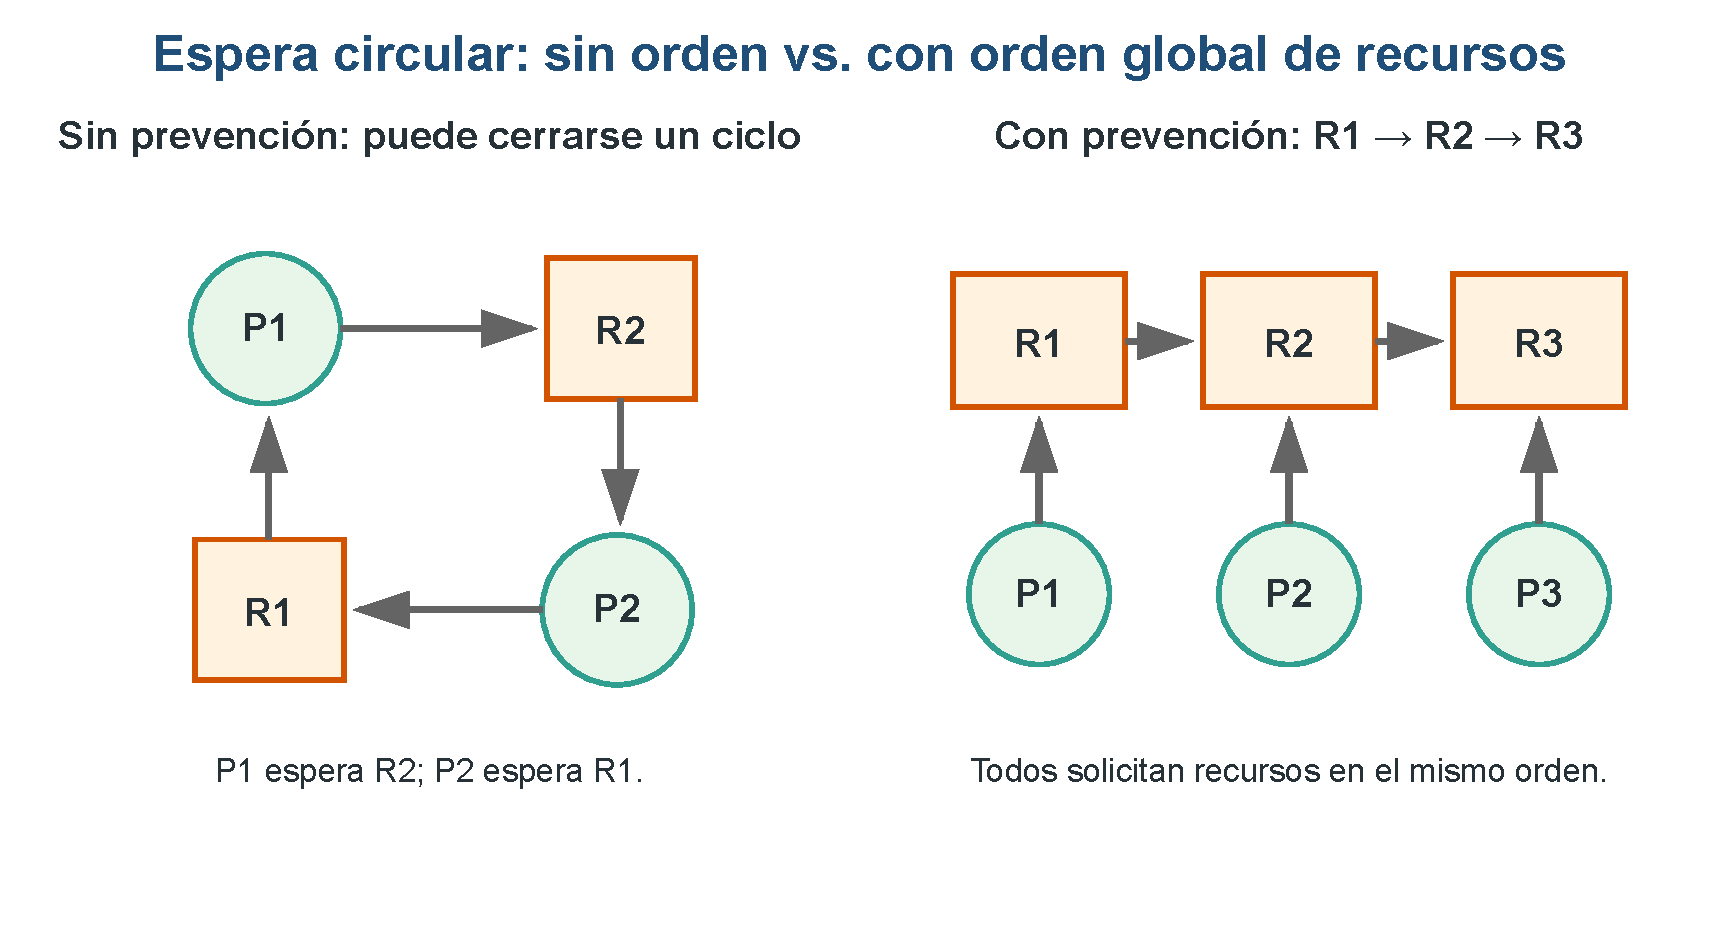
\includegraphics[width=0.94\linewidth,height=\textheight,keepaspectratio]{index_files/mediabag/capitulos/img/prevencion_interbloqueos/espera_circular_orden.pdf}

Si todos siguen el mismo orden, un proceso no puede solicitar un recurso
anterior después de haber obtenido uno posterior. Esto impide cerrar el
ciclo de espera.

\subsection{Ejercicio rápido}\label{ejercicio-ruxe1pido}

Un sistema define:

\begin{Shaded}
\begin{Highlighting}[]
\NormalTok{R1 = Archivo}
\NormalTok{R2 = Base de datos}
\NormalTok{R3 = Impresora}
\end{Highlighting}
\end{Shaded}

Analiza estas solicitudes:

\begin{Shaded}
\begin{Highlighting}[]
\NormalTok{P1: R1 → R2}
\NormalTok{P2: R2 → R3}
\NormalTok{P3: R3 → R1}
\end{Highlighting}
\end{Shaded}

\begin{enumerate}
\def\labelenumi{\arabic{enumi}.}
\tightlist
\item
  ¿Qué proceso viola el orden establecido?
\item
  ¿Qué podría ocurrir si permitimos esa solicitud?
\item
  ¿Cómo debería solicitar P3 sus recursos?
\end{enumerate}

\begin{tcolorbox}[enhanced jigsaw, arc=.35mm, bottomrule=.15mm, bottomtitle=1mm, breakable, colback=white, colbacktitle=quarto-callout-tip-color!10!white, colframe=quarto-callout-tip-color-frame, coltitle=black, left=2mm, leftrule=.75mm, opacityback=0, opacitybacktitle=0.6, rightrule=.15mm, title=\textcolor{quarto-callout-tip-color}{\faLightbulb}\hspace{0.5em}{✅ Ver solución}, titlerule=0mm, toprule=.15mm, toptitle=1mm]

El orden global establecido es \textbf{R1 → R2 → R3}.

\begin{itemize}
\tightlist
\item
  \textbf{P1: R1 → R2}: respeta el orden.
\item
  \textbf{P2: R2 → R3}: respeta el orden.
\item
  \textbf{P3: R3 → R1}: \textbf{viola el orden}, porque después de R3
  intenta solicitar un recurso anterior.
\end{itemize}

Si permitimos esa solicitud puede cerrarse una cadena circular entre
procesos y recursos, creando las condiciones para un interbloqueo.

P3 debería solicitar sus recursos en orden ascendente: \textbf{R1 → R3},
y no \textbf{R3 → R1}.

\textbf{Idea clave:} imponer un orden global rompe la condición de
\textbf{espera circular}.

\end{tcolorbox}

\begin{center}\rule{0.5\linewidth}{0.5pt}\end{center}

\bookmarksetup{startatroot}

\chapter{7. Prevención, evitación y detección no son lo
mismo}\label{prevenciuxf3n-evitaciuxf3n-y-detecciuxf3n-no-son-lo-mismo}

{\def\LTcaptype{none} % do not increment counter
\begin{longtable}[]{@{}
  >{\raggedright\arraybackslash}p{(\linewidth - 2\tabcolsep) * \real{0.5000}}
  >{\raggedright\arraybackslash}p{(\linewidth - 2\tabcolsep) * \real{0.5000}}@{}}
\toprule\noalign{}
\begin{minipage}[b]{\linewidth}\raggedright
Estrategia
\end{minipage} & \begin{minipage}[b]{\linewidth}\raggedright
Idea
\end{minipage} \\
\midrule\noalign{}
\endhead
\bottomrule\noalign{}
\endlastfoot
Prevención & Diseñar reglas para que alguna condición necesaria no pueda
cumplirse \\
Evitación & Evaluar cada asignación y concederla solo si el sistema
permanece en un estado seguro \\
Detección & Permitir la ejecución y buscar posteriormente si apareció un
interbloqueo \\
Recuperación & Tomar acciones después de detectar el interbloqueo \\
\end{longtable}
}

\begin{tcolorbox}[enhanced jigsaw, arc=.35mm, bottomrule=.15mm, bottomtitle=1mm, breakable, colback=white, colbacktitle=quarto-callout-tip-color!10!white, colframe=quarto-callout-tip-color-frame, coltitle=black, left=2mm, leftrule=.75mm, opacityback=0, opacitybacktitle=0.6, rightrule=.15mm, title=\textcolor{quarto-callout-tip-color}{\faLightbulb}\hspace{0.5em}{Precisión importante}, titlerule=0mm, toprule=.15mm, toptitle=1mm]

El material de clase introduce el \textbf{algoritmo del banquero} dentro
de las estrategias para impedir interbloqueos. Técnicamente, suele
clasificarse como un algoritmo de \textbf{evitación}, porque no elimina
permanentemente una condición: analiza si conceder una solicitud
mantiene al sistema en un estado seguro.

\end{tcolorbox}

\begin{center}\rule{0.5\linewidth}{0.5pt}\end{center}

\bookmarksetup{startatroot}

\chapter{8. Detección de
interbloqueos}\label{detecciuxf3n-de-interbloqueos}

En la detección, el sistema \textbf{no impide necesariamente} que se
forme un interbloqueo.

En cambio:

\begin{enumerate}
\def\labelenumi{\arabic{enumi}.}
\tightlist
\item
  permite que los procesos soliciten y reciban recursos;
\item
  analiza periódicamente el estado del sistema;
\item
  busca dependencias que indiquen bloqueo;
\item
  si encuentra un interbloqueo, inicia una estrategia de recuperación.
\end{enumerate}

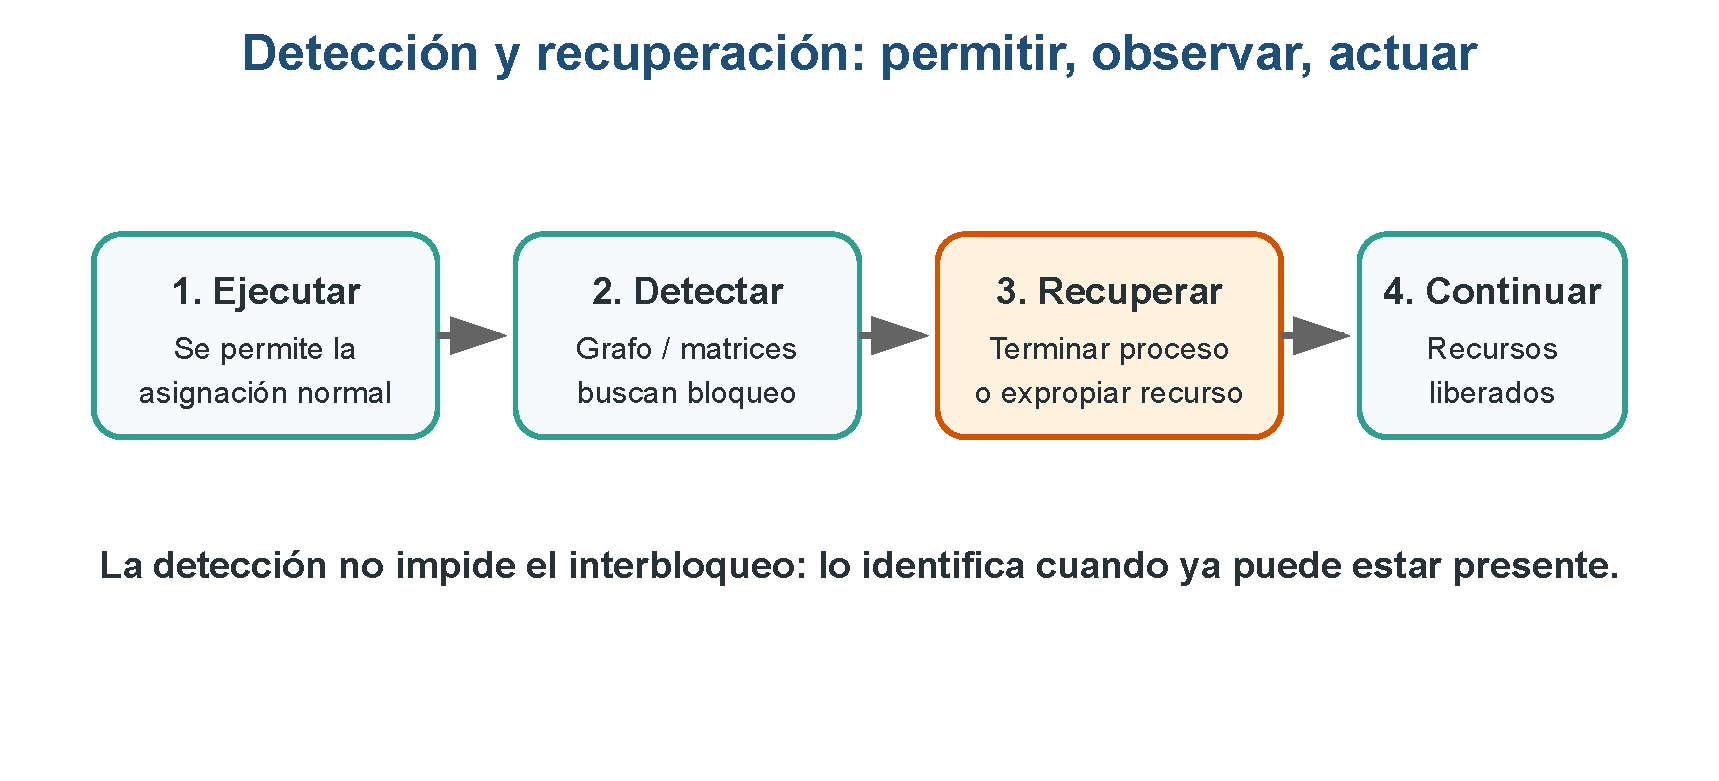
\includegraphics[width=0.92\linewidth,height=\textheight,keepaspectratio]{index_files/mediabag/capitulos/img/prevencion_interbloqueos/deteccion_recuperacion.pdf}

\begin{center}\rule{0.5\linewidth}{0.5pt}\end{center}

\bookmarksetup{startatroot}

\chapter{9. Grafo de asignación de
recursos}\label{grafo-de-asignaciuxf3n-de-recursos}

Un grafo de asignación representa:

\begin{itemize}
\tightlist
\item
  \textbf{procesos} mediante círculos;
\item
  \textbf{recursos} mediante cuadros;
\item
  \texttt{P\ →\ R} cuando un proceso solicita un recurso;
\item
  \texttt{R\ →\ P} cuando un recurso está asignado a un proceso.
\end{itemize}

Ejemplo:

\begin{Shaded}
\begin{Highlighting}[]
\NormalTok{P1 → R2}
\NormalTok{R2 → P2}
\NormalTok{P2 → R3}
\NormalTok{R3 → P1}
\end{Highlighting}
\end{Shaded}

La cadena vuelve a P1:

\begin{Shaded}
\begin{Highlighting}[]
\NormalTok{P1 → R2 → P2 → R3 → P1}
\end{Highlighting}
\end{Shaded}

Existe un ciclo.

\begin{tcolorbox}[enhanced jigsaw, arc=.35mm, bottomrule=.15mm, bottomtitle=1mm, breakable, colback=white, colbacktitle=quarto-callout-note-color!10!white, colframe=quarto-callout-note-color-frame, coltitle=black, left=2mm, leftrule=.75mm, opacityback=0, opacitybacktitle=0.6, rightrule=.15mm, title=\textcolor{quarto-callout-note-color}{\faInfo}\hspace{0.5em}{Importante}, titlerule=0mm, toprule=.15mm, toptitle=1mm]

En el caso simple donde cada tipo de recurso tiene una sola instancia,
un ciclo confirma el interbloqueo. Con múltiples instancias, la
interpretación requiere un análisis adicional.

\end{tcolorbox}

\section{Practiquemos}\label{practiquemos}

Analiza:

\begin{Shaded}
\begin{Highlighting}[]
\NormalTok{R1 → P1}
\NormalTok{P1 → R2}
\NormalTok{R2 → P2}
\NormalTok{P2 → R1}
\end{Highlighting}
\end{Shaded}

Responde:

\begin{enumerate}
\def\labelenumi{\arabic{enumi}.}
\tightlist
\item
  ¿Qué recurso posee P1?
\item
  ¿Qué recurso solicita P1?
\item
  ¿Qué recurso posee P2?
\item
  ¿Qué recurso solicita P2?
\item
  ¿Existe un ciclo?
\item
  ¿Existe interbloqueo en este caso?
\end{enumerate}

\begin{tcolorbox}[enhanced jigsaw, arc=.35mm, bottomrule=.15mm, bottomtitle=1mm, breakable, colback=white, colbacktitle=quarto-callout-tip-color!10!white, colframe=quarto-callout-tip-color-frame, coltitle=black, left=2mm, leftrule=.75mm, opacityback=0, opacitybacktitle=0.6, rightrule=.15mm, title=\textcolor{quarto-callout-tip-color}{\faLightbulb}\hspace{0.5em}{✅ Ver solución}, titlerule=0mm, toprule=.15mm, toptitle=1mm]

\begin{enumerate}
\def\labelenumi{\arabic{enumi}.}
\tightlist
\item
  P1 posee \textbf{R1}.
\item
  P1 solicita \textbf{R2}.
\item
  P2 posee \textbf{R2}.
\item
  P2 solicita \textbf{R1}.
\item
  Sí existe un ciclo: \textbf{R1 → P1 → R2 → P2 → R1}.
\item
  Si R1 y R2 tienen \textbf{una sola instancia cada uno}, sí existe
  interbloqueo: P1 espera R2, que posee P2, mientras P2 espera R1, que
  posee P1.
\end{enumerate}

\textbf{Importante:} con una sola instancia por tipo de recurso, el
ciclo confirma el interbloqueo. Con múltiples instancias se necesita un
análisis adicional.

\end{tcolorbox}

\begin{center}\rule{0.5\linewidth}{0.5pt}\end{center}

\bookmarksetup{startatroot}

\chapter{10. El algoritmo del banquero}\label{el-algoritmo-del-banquero}

El algoritmo del banquero fue propuesto por \textbf{Edsger Dijkstra}.

Su idea puede imaginarse como un banco que presta dinero:

\begin{quote}
El banco no concede un préstamo únicamente porque tenga dinero
disponible en este instante. Antes debe comprobar que, después del
préstamo, todavía existe una forma de satisfacer a todos sus clientes.
\end{quote}

En Sistemas Operativos:

\begin{itemize}
\tightlist
\item
  los clientes son \textbf{procesos};
\item
  el dinero representa \textbf{recursos};
\item
  cada proceso declara su necesidad máxima;
\item
  el sistema analiza si una asignación mantiene un \textbf{estado
  seguro}.
\end{itemize}

\begin{center}\rule{0.5\linewidth}{0.5pt}\end{center}

\bookmarksetup{startatroot}

\chapter{11. ¿Qué es un estado
seguro?}\label{quuxe9-es-un-estado-seguro}

Un estado es \textbf{seguro} cuando existe al menos una secuencia de
ejecución en la cual todos los procesos pueden terminar.

Supongamos tres procesos:

\begin{Shaded}
\begin{Highlighting}[]
\NormalTok{P1}
\NormalTok{P2}
\NormalTok{P3}
\end{Highlighting}
\end{Shaded}

Si existe una secuencia como:

\begin{Shaded}
\begin{Highlighting}[]
\NormalTok{P2 → P1 → P3}
\end{Highlighting}
\end{Shaded}

en la cual P2 puede terminar con los recursos disponibles, liberar los
suyos, luego P1 puede terminar y finalmente P3, entonces tenemos una
\textbf{secuencia segura}.

\begin{tcolorbox}[enhanced jigsaw, arc=.35mm, bottomrule=.15mm, bottomtitle=1mm, breakable, colback=white, colbacktitle=quarto-callout-important-color!10!white, colframe=quarto-callout-important-color-frame, coltitle=black, left=2mm, leftrule=.75mm, opacityback=0, opacitybacktitle=0.6, rightrule=.15mm, title=\textcolor{quarto-callout-important-color}{\faExclamation}\hspace{0.5em}{Estado inseguro ≠ interbloqueo actual}, titlerule=0mm, toprule=.15mm, toptitle=1mm]

Un estado inseguro significa que el sistema ya no puede garantizar una
secuencia segura.

No significa necesariamente que el interbloqueo ya ocurrió, pero existe
riesgo de llegar a él.

\end{tcolorbox}

\begin{center}\rule{0.5\linewidth}{0.5pt}\end{center}

\bookmarksetup{startatroot}

\chapter{12. Ejemplo básico del
banquero}\label{ejemplo-buxe1sico-del-banquero}

Consideremos un solo tipo de recurso para comprender primero la lógica.

El sistema tiene \textbf{10 unidades}.

{\def\LTcaptype{none} % do not increment counter
\begin{longtable}[]{@{}lrrr@{}}
\toprule\noalign{}
Proceso & Asignado & Máximo & Necesita todavía \\
\midrule\noalign{}
\endhead
\bottomrule\noalign{}
\endlastfoot
P1 & 3 & 7 & 4 \\
P2 & 2 & 4 & 2 \\
P3 & 2 & 5 & 3 \\
\end{longtable}
}

Recursos utilizados:

\begin{Shaded}
\begin{Highlighting}[]
\NormalTok{3 + 2 + 2 = 7}
\end{Highlighting}
\end{Shaded}

Recursos disponibles:

\begin{Shaded}
\begin{Highlighting}[]
\NormalTok{10 {-} 7 = 3}
\end{Highlighting}
\end{Shaded}

Preguntemos:

\begin{quote}
¿Existe algún proceso que pueda terminar necesitando como máximo las 3
unidades disponibles?
\end{quote}

P2 necesita 2.

Entonces:

\begin{enumerate}
\def\labelenumi{\arabic{enumi}.}
\tightlist
\item
  P2 recibe lo necesario y termina.
\item
  Libera sus recursos.
\item
  Ahora existen más recursos disponibles.
\item
  Buscamos otro proceso que pueda terminar.
\item
  Repetimos hasta completar todos los procesos.
\end{enumerate}

\begin{tcolorbox}[enhanced jigsaw, arc=.35mm, bottomrule=.15mm, bottomtitle=1mm, breakable, colback=white, colbacktitle=quarto-callout-note-color!10!white, colframe=quarto-callout-note-color-frame, coltitle=black, left=2mm, leftrule=.75mm, opacityback=0, opacitybacktitle=0.6, rightrule=.15mm, title=\textcolor{quarto-callout-note-color}{\faInfo}\hspace{0.5em}{Ejercicio guiado}, titlerule=0mm, toprule=.15mm, toptitle=1mm]

Continúa el ejemplo:

\begin{enumerate}
\def\labelenumi{\arabic{enumi}.}
\tightlist
\item
  Después de que P2 termina, ¿cuántos recursos quedan disponibles?
\item
  ¿Puede terminar P1?
\item
  ¿Puede terminar P3?
\item
  Escribe una posible secuencia segura.
\end{enumerate}

\end{tcolorbox}

\begin{tcolorbox}[enhanced jigsaw, arc=.35mm, bottomrule=.15mm, bottomtitle=1mm, breakable, colback=white, colbacktitle=quarto-callout-tip-color!10!white, colframe=quarto-callout-tip-color-frame, coltitle=black, left=2mm, leftrule=.75mm, opacityback=0, opacitybacktitle=0.6, rightrule=.15mm, title=\textcolor{quarto-callout-tip-color}{\faLightbulb}\hspace{0.5em}{✅ Ver solución}, titlerule=0mm, toprule=.15mm, toptitle=1mm]

Inicialmente hay \textbf{3 recursos disponibles}.

\begin{itemize}
\tightlist
\item
  P2 necesita 2, por lo que puede recibirlos y terminar.
\item
  Al terminar P2 libera sus \textbf{4 recursos} en total (los 2 que
  tenía más los 2 que recibió). Como antes de atenderlo había 3
  disponibles, después quedan \textbf{5 disponibles}.
\item
  P1 necesita 4, así que ahora puede terminar. Al liberar sus 7
  recursos, quedan \textbf{10 disponibles}.
\item
  Finalmente P3, que necesita 3, también puede terminar.
\end{itemize}

Una secuencia segura posible es:

\textbf{P2 → P1 → P3}

También puede existir otra secuencia segura; lo importante es demostrar
que existe al menos una en la que todos los procesos puedan finalizar.

\end{tcolorbox}

\begin{center}\rule{0.5\linewidth}{0.5pt}\end{center}

\bookmarksetup{startatroot}

\chapter{13. Actividad por pares: ¿cómo lo
resolverías?}\label{actividad-por-pares-cuxf3mo-lo-resolveruxedas}

Analicen:

\begin{Shaded}
\begin{Highlighting}[]
\NormalTok{Proceso A tiene Disco y solicita Memoria.}
\NormalTok{Proceso B tiene Memoria y solicita Disco.}
\end{Highlighting}
\end{Shaded}

Respondan:

\begin{enumerate}
\def\labelenumi{\arabic{enumi}.}
\tightlist
\item
  ¿Qué condiciones de interbloqueo se cumplen?
\item
  ¿Existe espera circular?
\item
  ¿Qué política de prevención podría evitar el problema?
\item
  Si el interbloqueo ya ocurrió, ¿qué recurso podría intentarse
  recuperar?
\item
  ¿Qué riesgo tendría expropiar un recurso?
\end{enumerate}

Tiempo sugerido: \textbf{5 minutos}.

\begin{tcolorbox}[enhanced jigsaw, arc=.35mm, bottomrule=.15mm, bottomtitle=1mm, breakable, colback=white, colbacktitle=quarto-callout-tip-color!10!white, colframe=quarto-callout-tip-color-frame, coltitle=black, left=2mm, leftrule=.75mm, opacityback=0, opacitybacktitle=0.6, rightrule=.15mm, title=\textcolor{quarto-callout-tip-color}{\faLightbulb}\hspace{0.5em}{✅ Ver solución}, titlerule=0mm, toprule=.15mm, toptitle=1mm]

\begin{enumerate}
\def\labelenumi{\arabic{enumi}.}
\tightlist
\item
  \textbf{Se cumplen las cuatro condiciones:} exclusión mutua, retención
  y espera, no expropiación y espera circular.
\item
  \textbf{Sí existe espera circular:} A espera Memoria, que posee B; B
  espera Disco, que posee A.
\item
  Una política sencilla sería imponer un \textbf{orden global de
  recursos}, por ejemplo: \textbf{Disco → Memoria}. Todos los procesos
  que necesiten ambos deberán solicitarlos en ese orden.
\item
  Si el interbloqueo ya ocurrió, podría intentarse recuperar uno de los
  recursos \textbf{solo si puede expropiarse de forma segura}. Otra
  alternativa es finalizar o reiniciar uno de los procesos para que
  libere lo que posee.
\item
  Expropiar un recurso puede dejar al proceso en un estado
  inconsistente, provocar pérdida de trabajo o exigir repetir
  operaciones.
\end{enumerate}

\textbf{Conclusión:} prevenir el ciclo suele ser menos costoso que
recuperarse después de que el interbloqueo ya ocurrió.

\end{tcolorbox}

\begin{center}\rule{0.5\linewidth}{0.5pt}\end{center}

\bookmarksetup{startatroot}

\chapter{14. Recuperación después del
interbloqueo}\label{recuperaciuxf3n-despuuxe9s-del-interbloqueo}

Si el interbloqueo ya existe, prevenirlo dejó de ser una opción. Debemos
recuperarnos.

Dos estrategias comunes son:

\section{Finalizar procesos}\label{finalizar-procesos}

El Sistema Operativo puede:

\begin{itemize}
\tightlist
\item
  terminar todos los procesos involucrados, o
\item
  terminar procesos uno por uno hasta romper el ciclo.
\end{itemize}

\section{Retirar recursos
selectivamente}\label{retirar-recursos-selectivamente}

El sistema puede intentar expropiar un recurso y reasignarlo.

Para elegir una \textbf{víctima} deben considerarse factores como:

\begin{itemize}
\tightlist
\item
  prioridad del proceso;
\item
  tiempo que lleva ejecutándose;
\item
  cantidad de trabajo realizado;
\item
  recursos que posee;
\item
  costo de reiniciarlo;
\item
  riesgo de pérdida o inconsistencia de datos.
\end{itemize}

\begin{center}\rule{0.5\linewidth}{0.5pt}\end{center}

\bookmarksetup{startatroot}

\chapter{15. Caso integrador}\label{caso-integrador-2}

Un servidor tiene:

\begin{Shaded}
\begin{Highlighting}[]
\NormalTok{P1: posee Archivo A y solicita Impresora}
\NormalTok{P2: posee Impresora y solicita Archivo A}
\end{Highlighting}
\end{Shaded}

Trabajemos en cuatro niveles.

\section{Nivel 1. Diagnóstico}\label{nivel-1.-diagnuxf3stico}

\begin{itemize}
\tightlist
\item
  ¿Existe interbloqueo?
\item
  ¿Cuáles condiciones se cumplen?
\end{itemize}

\section{Nivel 2. Prevención}\label{nivel-2.-prevenciuxf3n}

\begin{itemize}
\tightlist
\item
  ¿Qué condición podríamos romper?
\item
  ¿Cómo impondríamos un orden de recursos?
\end{itemize}

\section{Nivel 3. Detección}\label{nivel-3.-detecciuxf3n}

Dibuja el grafo utilizando:

\begin{Shaded}
\begin{Highlighting}[]
\NormalTok{Proceso → Recurso solicitado}
\NormalTok{Recurso → Proceso que lo posee}
\end{Highlighting}
\end{Shaded}

\section{Nivel 4. Recuperación}\label{nivel-4.-recuperaciuxf3n}

Si ya ocurrió:

\begin{itemize}
\tightlist
\item
  ¿terminarías P1 o P2?
\item
  ¿intentarías retirar un recurso?
\item
  ¿qué información necesitarías para decidir?
\end{itemize}

\begin{tcolorbox}[enhanced jigsaw, arc=.35mm, bottomrule=.15mm, bottomtitle=1mm, breakable, colback=white, colbacktitle=quarto-callout-tip-color!10!white, colframe=quarto-callout-tip-color-frame, coltitle=black, left=2mm, leftrule=.75mm, opacityback=0, opacitybacktitle=0.6, rightrule=.15mm, title=\textcolor{quarto-callout-tip-color}{\faLightbulb}\hspace{0.5em}{✅ Ver solución}, titlerule=0mm, toprule=.15mm, toptitle=1mm]

\subsection{Nivel 1. Diagnóstico}\label{nivel-1.-diagnuxf3stico-1}

Sí existe interbloqueo, suponiendo que \textbf{Archivo A} y la
\textbf{Impresora} son recursos exclusivos con una sola instancia. Se
cumplen las cuatro condiciones: exclusión mutua, retención y espera, no
expropiación y espera circular.

\subsection{Nivel 2. Prevención}\label{nivel-2.-prevenciuxf3n-1}

Podemos romper la \textbf{espera circular} imponiendo un orden global,
por ejemplo:

\begin{Shaded}
\begin{Highlighting}[]
\NormalTok{Archivo A → Impresora}
\end{Highlighting}
\end{Shaded}

Todos los procesos que necesiten ambos recursos deberán solicitarlos en
ese mismo orden.

\subsection{Nivel 3. Detección}\label{nivel-3.-detecciuxf3n-1}

El grafo contiene:

\begin{Shaded}
\begin{Highlighting}[]
\NormalTok{Archivo A → P1}
\NormalTok{P1 → Impresora}
\NormalTok{Impresora → P2}
\NormalTok{P2 → Archivo A}
\end{Highlighting}
\end{Shaded}

Por tanto aparece el ciclo:

\begin{Shaded}
\begin{Highlighting}[]
\NormalTok{Archivo A → P1 → Impresora → P2 → Archivo A}
\end{Highlighting}
\end{Shaded}

Con una sola instancia de cada recurso, el ciclo representa un
interbloqueo.

\subsection{Nivel 4. Recuperación}\label{nivel-4.-recuperaciuxf3n-1}

No podemos decidir automáticamente si conviene terminar P1 o P2
únicamente con la información del enunciado. Para elegir una víctima
deberíamos considerar, entre otros factores:

\begin{itemize}
\tightlist
\item
  prioridad de cada proceso;
\item
  cantidad de trabajo realizado;
\item
  costo de reiniciarlo;
\item
  recursos que liberaría;
\item
  consecuencias de cancelar la operación;
\item
  posibilidad de repetir o recuperar el trabajo.
\end{itemize}

También podría intentarse expropiar un recurso si la operación permite
hacerlo de manera segura.

\textbf{Idea clave:} detectar el interbloqueo no resuelve el problema
por sí solo; la recuperación puede tener un costo importante.

\end{tcolorbox}

\begin{center}\rule{0.5\linewidth}{0.5pt}\end{center}

\bookmarksetup{startatroot}

\chapter{16. Actividad individual}\label{actividad-individual}

Busca un caso real o documentado de interbloqueo en software.

Identifica:

\begin{enumerate}
\def\labelenumi{\arabic{enumi}.}
\tightlist
\item
  ¿Qué procesos o hilos estaban involucrados?
\item
  ¿Qué recursos estaban utilizando?
\item
  ¿Cómo se produjo la espera?
\item
  ¿Cómo se detectó?
\item
  ¿Cómo se solucionó o evitó posteriormente?
\end{enumerate}

\begin{tcolorbox}[enhanced jigsaw, arc=.35mm, bottomrule=.15mm, bottomtitle=1mm, breakable, colback=white, colbacktitle=quarto-callout-tip-color!10!white, colframe=quarto-callout-tip-color-frame, coltitle=black, left=2mm, leftrule=.75mm, opacityback=0, opacitybacktitle=0.6, rightrule=.15mm, title=\textcolor{quarto-callout-tip-color}{\faLightbulb}\hspace{0.5em}{No basta con encontrar el caso}, titlerule=0mm, toprule=.15mm, toptitle=1mm]

Debes poder relacionarlo con al menos una de estas ideas:

\textbf{prevención -- evitación -- detección -- recuperación}

\end{tcolorbox}

\begin{center}\rule{0.5\linewidth}{0.5pt}\end{center}

\bookmarksetup{startatroot}

\chapter{17. Autoevaluación}\label{autoevaluaciuxf3n-6}

\begin{enumerate}
\def\labelenumi{\arabic{enumi}.}
\tightlist
\item
  ¿Cuál es la idea fundamental de la prevención de interbloqueos?
\item
  ¿Cómo puede atacarse la condición de retención y espera?
\item
  ¿Qué desventaja tiene solicitar todos los recursos al inicio?
\item
  ¿Qué significa expropiar un recurso?
\item
  ¿Por qué algunos recursos no deberían expropiarse?
\item
  ¿Cómo evita un orden global de recursos la espera circular?
\item
  ¿Qué diferencia existe entre prevención y detección?
\item
  ¿Qué representa \texttt{P\ →\ R} en un grafo de asignación?
\item
  ¿Qué representa \texttt{R\ →\ P}?
\item
  ¿Qué es un estado seguro?
\item
  ¿Por qué el algoritmo del banquero se relaciona con la evitación?
\item
  ¿Qué alternativas existen para recuperarse de un interbloqueo?
\end{enumerate}

\begin{center}\rule{0.5\linewidth}{0.5pt}\end{center}

\bookmarksetup{startatroot}

\chapter{18. Resumen del capítulo}\label{resumen-del-capuxedtulo-3}

En este capítulo aprendimos que no existe una única estrategia frente a
los interbloqueos.

Podemos actuar \textbf{antes}, \textbf{durante} o \textbf{después} del
problema:

\begin{Shaded}
\begin{Highlighting}[]
\NormalTok{PREVENIR  → romper una condición necesaria}
\NormalTok{EVITAR    → conceder recursos solo si el estado continúa siendo seguro}
\NormalTok{DETECTAR  → buscar interbloqueos durante la ejecución}
\NormalTok{RECUPERAR → romper el bloqueo después de detectarlo}
\end{Highlighting}
\end{Shaded}

También estudiamos:

\begin{itemize}
\tightlist
\item
  retención y espera;
\item
  expropiación;
\item
  espera circular;
\item
  grafos de asignación;
\item
  estados seguros;
\item
  algoritmo del banquero;
\item
  finalización de procesos;
\item
  recuperación de recursos.
\end{itemize}

\begin{tcolorbox}[enhanced jigsaw, arc=.35mm, bottomrule=.15mm, bottomtitle=1mm, breakable, colback=white, colbacktitle=quarto-callout-note-color!10!white, colframe=quarto-callout-note-color-frame, coltitle=black, left=2mm, leftrule=.75mm, opacityback=0, opacitybacktitle=0.6, rightrule=.15mm, title=\textcolor{quarto-callout-note-color}{\faInfo}\hspace{0.5em}{Para recordar}, titlerule=0mm, toprule=.15mm, toptitle=1mm]

La mejor estrategia depende del tipo de sistema, del costo de mantener
recursos reservados y de las consecuencias de detener o reiniciar
procesos.

\end{tcolorbox}

\begin{center}\rule{0.5\linewidth}{0.5pt}\end{center}

\bookmarksetup{startatroot}

\chapter{Conexión con la siguiente
clase}\label{conexiuxf3n-con-la-siguiente-clase}

Ya sabemos:

\begin{itemize}
\tightlist
\item
  cómo se forma un interbloqueo;
\item
  cómo prevenirlo;
\item
  cómo analizar estados seguros;
\item
  cómo detectarlo;
\item
  y qué opciones existen para recuperarse.
\end{itemize}

En la siguiente etapa podremos profundizar en la administración de
recursos y en los mecanismos que utiliza el Sistema Operativo para
coordinar procesos concurrentes.

\begin{center}\rule{0.5\linewidth}{0.5pt}\end{center}

\bookmarksetup{startatroot}

\chapter{Bibliografía base}\label{bibliografuxeda-base-1}

De acuerdo con el material de clase:

\begin{itemize}
\tightlist
\item
  Tanenbaum, secciones/capítulos 7.2--7.4 indicados en la presentación.
\item
  Deitel, secciones/capítulos 5.2--5.4 indicados en la presentación.
\item
  Capítulo anterior: \textbf{Condiciones necesarias de interbloqueo}.
\end{itemize}

\bookmarksetup{startatroot}

\chapter{Actividad - Diagnóstico de un Sistema
Operativo}\label{actividad---diagnuxf3stico-de-un-sistema-operativo}

\thispagestyle{empty}

\bookmarksetup{startatroot}

\chapter{Universidad Mariano Gálvez de
Guatemala}\label{universidad-mariano-guxe1lvez-de-guatemala}

\textbf{Facultad de Ingeniería en Sistemas}\\
\textbf{Curso:} Sistemas Operativos I\\
\textbf{Docente:} Ing. Jorge Luis García Chacón\\
\textbf{Actividad:} Diagnóstico de un Sistema Operativo\\
\textbf{Valor:} 25 puntos\\
\textbf{Modalidad:} Trabajo en grupo\\
\textbf{Tiempo estimado:} 60 minutos

\textbf{Grupo No.:} \_\_\_\_\_\_\_\_\_\_\_\_\_\_\_\_\_\_\_\_

\textbf{Integrantes:}

\begin{enumerate}
\def\labelenumi{\arabic{enumi}.}
\item
  \begin{center}\rule{0.5\linewidth}{0.5pt}\end{center}
\item
  \begin{center}\rule{0.5\linewidth}{0.5pt}\end{center}
\item
  \begin{center}\rule{0.5\linewidth}{0.5pt}\end{center}
\item
  \begin{center}\rule{0.5\linewidth}{0.5pt}\end{center}
\item
  \begin{center}\rule{0.5\linewidth}{0.5pt}\end{center}
\item
  \begin{center}\rule{0.5\linewidth}{0.5pt}\end{center}
\end{enumerate}

\begin{tcolorbox}[enhanced jigsaw, arc=.35mm, bottomrule=.15mm, bottomtitle=1mm, breakable, colback=white, colbacktitle=quarto-callout-important-color!10!white, colframe=quarto-callout-important-color-frame, coltitle=black, left=2mm, leftrule=.75mm, opacityback=0, opacitybacktitle=0.6, rightrule=.15mm, title=\textcolor{quarto-callout-important-color}{\faExclamation}\hspace{0.5em}{Reglas de trabajo}, titlerule=0mm, toprule=.15mm, toptitle=1mm]

\begin{itemize}
\tightlist
\item
  Esta actividad se resolverá \textbf{en papel} y en grupo.
\item
  Pueden consultar sus \textbf{apuntes o el libro del curso}.
\item
  No se permite utilizar teléfono, computadora ni herramientas de IA
  durante la actividad.
\item
  Todas las respuestas deben ser \textbf{razonadas}. No basta con
  escribir el nombre de un concepto.
\item
  El docente podrá pedir a cualquier integrante que explique una
  respuesta del grupo.
\end{itemize}

\end{tcolorbox}

\section{Escenario}\label{escenario-1}

En el laboratorio de cómputo de una universidad, una computadora
presenta problemas de rendimiento mientras varios usuarios realizan
distintas tareas. El encargado del laboratorio reporta lo siguiente:

\begin{itemize}
\tightlist
\item
  El equipo tarda en responder cuando se cambia entre aplicaciones.
\item
  Un navegador mantiene varias pestañas abiertas y reproduce video.
\item
  Un estudiante está descargando un archivo grande desde Internet.
\item
  Otro programa está enviando un documento a imprimir.
\item
  El antivirus realiza una revisión en segundo plano.
\item
  En algunos momentos una aplicación deja de responder durante varios
  segundos y luego continúa.
\end{itemize}

El administrador consulta el estado del sistema y obtiene la siguiente
información:

{\def\LTcaptype{none} % do not increment counter
\begin{longtable}[]{@{}
  >{\raggedright\arraybackslash}p{(\linewidth - 8\tabcolsep) * \real{0.1765}}
  >{\raggedright\arraybackslash}p{(\linewidth - 8\tabcolsep) * \real{0.1765}}
  >{\raggedleft\arraybackslash}p{(\linewidth - 8\tabcolsep) * \real{0.2353}}
  >{\raggedleft\arraybackslash}p{(\linewidth - 8\tabcolsep) * \real{0.2353}}
  >{\raggedright\arraybackslash}p{(\linewidth - 8\tabcolsep) * \real{0.1765}}@{}}
\toprule\noalign{}
\begin{minipage}[b]{\linewidth}\raggedright
Proceso
\end{minipage} & \begin{minipage}[b]{\linewidth}\raggedright
Estado observado
\end{minipage} & \begin{minipage}[b]{\linewidth}\raggedleft
CPU
\end{minipage} & \begin{minipage}[b]{\linewidth}\raggedleft
Memoria
\end{minipage} & \begin{minipage}[b]{\linewidth}\raggedright
Observación
\end{minipage} \\
\midrule\noalign{}
\endhead
\bottomrule\noalign{}
\endlastfoot
Navegador & Running & 55 \% & 1.8 GB & Varias pestañas y video activo \\
Descarga & Ready & 10 \% & 220 MB & Archivo grande en proceso \\
Procesador de texto & Ready & 4 \% & 650 MB & Documento abierto \\
Antivirus & Ready & 24 \% & 900 MB & Análisis en segundo plano \\
Impresión & Waiting & 0 \% & 85 MB & Esperando respuesta de la
impresora \\
Reproductor multimedia & Ready & 7 \% & 400 MB & Audio activo \\
\end{longtable}
}

La computadora posee \textbf{8 GB de RAM} y un procesador de \textbf{4
núcleos}.

\bookmarksetup{startatroot}

\chapter{Misión 1. Diagnóstico inicial --- 5
puntos}\label{misiuxf3n-1.-diagnuxf3stico-inicial-5-puntos}

Analicen la información disponible y respondan:

\textbf{1. ¿Cuál consideran que es el principal problema de rendimiento
del equipo?}\\
Justifiquen su respuesta utilizando la información del escenario y los
datos de los procesos.

\vspace{2.3cm}

\textbf{2. ¿Qué otros factores podrían estar contribuyendo al problema?}

\vspace{1.7cm}

\textbf{3. ¿Por qué no sería correcto afirmar inmediatamente que ``la
computadora está lenta porque la CPU está dañada''?}

\vspace{1.8cm}

\bookmarksetup{startatroot}

\chapter{Misión 2. ¿Qué ocurre dentro del Sistema Operativo? --- 5
puntos}\label{misiuxf3n-2.-quuxe9-ocurre-dentro-del-sistema-operativo-5-puntos}

Sin limitarse a definir conceptos, expliquen qué componentes o
mecanismos del Sistema Operativo intervienen en esta situación y
\textbf{qué papel cumplen}.

{\def\LTcaptype{none} % do not increment counter
\begin{longtable}[]{@{}
  >{\raggedright\arraybackslash}p{(\linewidth - 2\tabcolsep) * \real{0.5000}}
  >{\raggedright\arraybackslash}p{(\linewidth - 2\tabcolsep) * \real{0.5000}}@{}}
\toprule\noalign{}
\begin{minipage}[b]{\linewidth}\raggedright
Componente o mecanismo identificado
\end{minipage} & \begin{minipage}[b]{\linewidth}\raggedright
¿Qué está haciendo en este escenario?
\end{minipage} \\
\midrule\noalign{}
\endhead
\bottomrule\noalign{}
\endlastfoot
1. \_\_\_\_\_\_\_\_\_\_\_\_\_\_\_\_\_\_\_\_\_\_\_\_\_\_\_\_\_\_ & \\
2. \_\_\_\_\_\_\_\_\_\_\_\_\_\_\_\_\_\_\_\_\_\_\_\_\_\_\_\_\_\_ & \\
3. \_\_\_\_\_\_\_\_\_\_\_\_\_\_\_\_\_\_\_\_\_\_\_\_\_\_\_\_\_\_ & \\
4. \_\_\_\_\_\_\_\_\_\_\_\_\_\_\_\_\_\_\_\_\_\_\_\_\_\_\_\_\_\_ & \\
\end{longtable}
}

\newpage

\bookmarksetup{startatroot}

\chapter{Misión 3. Sigan un proceso --- 5
puntos}\label{misiuxf3n-3.-sigan-un-proceso-5-puntos}

Seleccionen el proceso \textbf{Impresión} y reconstruyan lo que
probablemente ocurre desde que el usuario solicita imprimir hasta que el
proceso vuelve a estar listo para continuar.

Dibujen los estados y transiciones que consideren necesarios.

\vspace{5cm}

\textbf{a. ¿Por qué el proceso de impresión aparece en estado
\texttt{Waiting}?}

\vspace{1.4cm}

\textbf{b. ¿Qué tendría que conservar el Sistema Operativo para poder
suspender temporalmente ese proceso y luego continuar su ejecución
correctamente?}

\vspace{1.8cm}

\textbf{c.~Cuando la impresora responde, ¿qué debería ocurrir con el
proceso? Expliquen la secuencia.}

\vspace{1.8cm}

\bookmarksetup{startatroot}

\chapter{Misión 4. Ustedes son el Sistema Operativo --- 5
puntos}\label{misiuxf3n-4.-ustedes-son-el-sistema-operativo-5-puntos}

Supongan ahora que la CPU debe atender los siguientes procesos:

{\def\LTcaptype{none} % do not increment counter
\begin{longtable}[]{@{}lrrl@{}}
\toprule\noalign{}
Proceso & Tiempo estimado de CPU & Prioridad & Tipo de trabajo \\
\midrule\noalign{}
\endhead
\bottomrule\noalign{}
\endlastfoot
P1 & 8 ms & 3 & Navegador interactivo \\
P2 & 2 ms & 1 & Proceso crítico del sistema \\
P3 & 6 ms & 2 & Antivirus \\
P4 & 3 ms & 3 & Reproductor multimedia \\
\end{longtable}
}

Respondan:

\textbf{1. ¿Qué criterio de planificación utilizarían para atender estos
procesos y por qué?}

\vspace{2cm}

\textbf{2. ¿Atenderían todos los procesos exactamente de la misma
manera? Justifiquen.}

\vspace{1.6cm}

\textbf{3. ¿Qué riesgo habría si un solo proceso pudiera conservar la
CPU durante demasiado tiempo?}

\vspace{1.6cm}

\newpage

\bookmarksetup{startatroot}

\chapter{Misión 5. Diagnóstico final --- 5
puntos}\label{misiuxf3n-5.-diagnuxf3stico-final-5-puntos}

\section{A. Recorrido de una
solicitud}\label{a.-recorrido-de-una-solicitud}

El usuario presiona \textbf{Imprimir} desde el procesador de texto.

Dibujen el recorrido que sigue esa solicitud desde el usuario hasta el
dispositivo físico. Incluyan únicamente los componentes que consideren
necesarios y expliquen brevemente qué ocurre en cada paso.

\vspace{5.5cm}

\section{B. Decisión final del
grupo}\label{b.-decisiuxf3n-final-del-grupo}

Como equipo responsable del diagnóstico, indiquen:

\textbf{1. ¿Qué acciones realizarían para mejorar el rendimiento del
equipo sin apagarlo inmediatamente?}

\vspace{2cm}

\textbf{2. ¿Qué proceso o recurso observarían primero y por qué?}

\vspace{1.5cm}

\textbf{3. Diagnóstico definitivo del grupo:}

\vspace{1.8cm}

\bookmarksetup{startatroot}

\chapter{Criterios de evaluación}\label{criterios-de-evaluaciuxf3n}

{\def\LTcaptype{none} % do not increment counter
\begin{longtable}[]{@{}lr@{}}
\toprule\noalign{}
Criterio & Punteo \\
\midrule\noalign{}
\endhead
\bottomrule\noalign{}
\endlastfoot
Diagnóstico y análisis del problema & 5 \\
Identificación y explicación de componentes del SO & 5 \\
Estados de procesos y razonamiento sobre el PCB & 5 \\
Decisión de planificación y justificación & 5 \\
Integración final: capas, diagnóstico y solución & 5 \\
\textbf{Total} & \textbf{25} \\
\end{longtable}
}

\begin{tcolorbox}[enhanced jigsaw, arc=.35mm, bottomrule=.15mm, bottomtitle=1mm, breakable, colback=white, colbacktitle=quarto-callout-note-color!10!white, colframe=quarto-callout-note-color-frame, coltitle=black, left=2mm, leftrule=.75mm, opacityback=0, opacitybacktitle=0.6, rightrule=.15mm, title=\textcolor{quarto-callout-note-color}{\faInfo}\hspace{0.5em}{Cierre}, titlerule=0mm, toprule=.15mm, toptitle=1mm]

La calidad de la respuesta se evaluará principalmente por la
\textbf{capacidad de análisis y justificación del grupo}, no por repetir
definiciones de memoria.

\end{tcolorbox}

\bookmarksetup{startatroot}

\chapter{Actividad - Diagnóstico de un Sistema
Operativo}\label{actividad---diagnuxf3stico-de-un-sistema-operativo-1}

Guía de respuestas y retroalimentación

\hfill\break

\bookmarksetup{startatroot}

\chapter{Antes de revisar las
respuestas}\label{antes-de-revisar-las-respuestas}

Esta guía se publica \textbf{después de realizar y exponer la
actividad}. Su propósito no es presentar una única respuesta posible,
sino comparar el razonamiento del grupo con una solución técnicamente
fundamentada.

\begin{tcolorbox}[enhanced jigsaw, arc=.35mm, bottomrule=.15mm, bottomtitle=1mm, breakable, colback=white, colbacktitle=quarto-callout-important-color!10!white, colframe=quarto-callout-important-color-frame, coltitle=black, left=2mm, leftrule=.75mm, opacityback=0, opacitybacktitle=0.6, rightrule=.15mm, title=\textcolor{quarto-callout-important-color}{\faExclamation}\hspace{0.5em}{Una idea importante}, titlerule=0mm, toprule=.15mm, toptitle=1mm]

En un diagnóstico real no siempre existe una sola respuesta correcta.
Una conclusión puede ser válida si utiliza correctamente la evidencia
disponible y puede justificarse.

\end{tcolorbox}

\bookmarksetup{startatroot}

\chapter{Recordemos el escenario}\label{recordemos-el-escenario}

El equipo tiene \textbf{8 GB de RAM}, un procesador de \textbf{4
núcleos} y varios procesos activos al mismo tiempo.

{\def\LTcaptype{none} % do not increment counter
\begin{longtable}[]{@{}llrr@{}}
\toprule\noalign{}
Proceso & Estado & CPU & Memoria \\
\midrule\noalign{}
\endhead
\bottomrule\noalign{}
\endlastfoot
Navegador & Running & 55 \% & 1.8 GB \\
Descarga & Ready & 10 \% & 220 MB \\
Procesador de texto & Ready & 4 \% & 650 MB \\
Antivirus & Ready & 24 \% & 900 MB \\
Impresión & Waiting & 0 \% & 85 MB \\
Reproductor multimedia & Ready & 7 \% & 400 MB \\
\end{longtable}
}

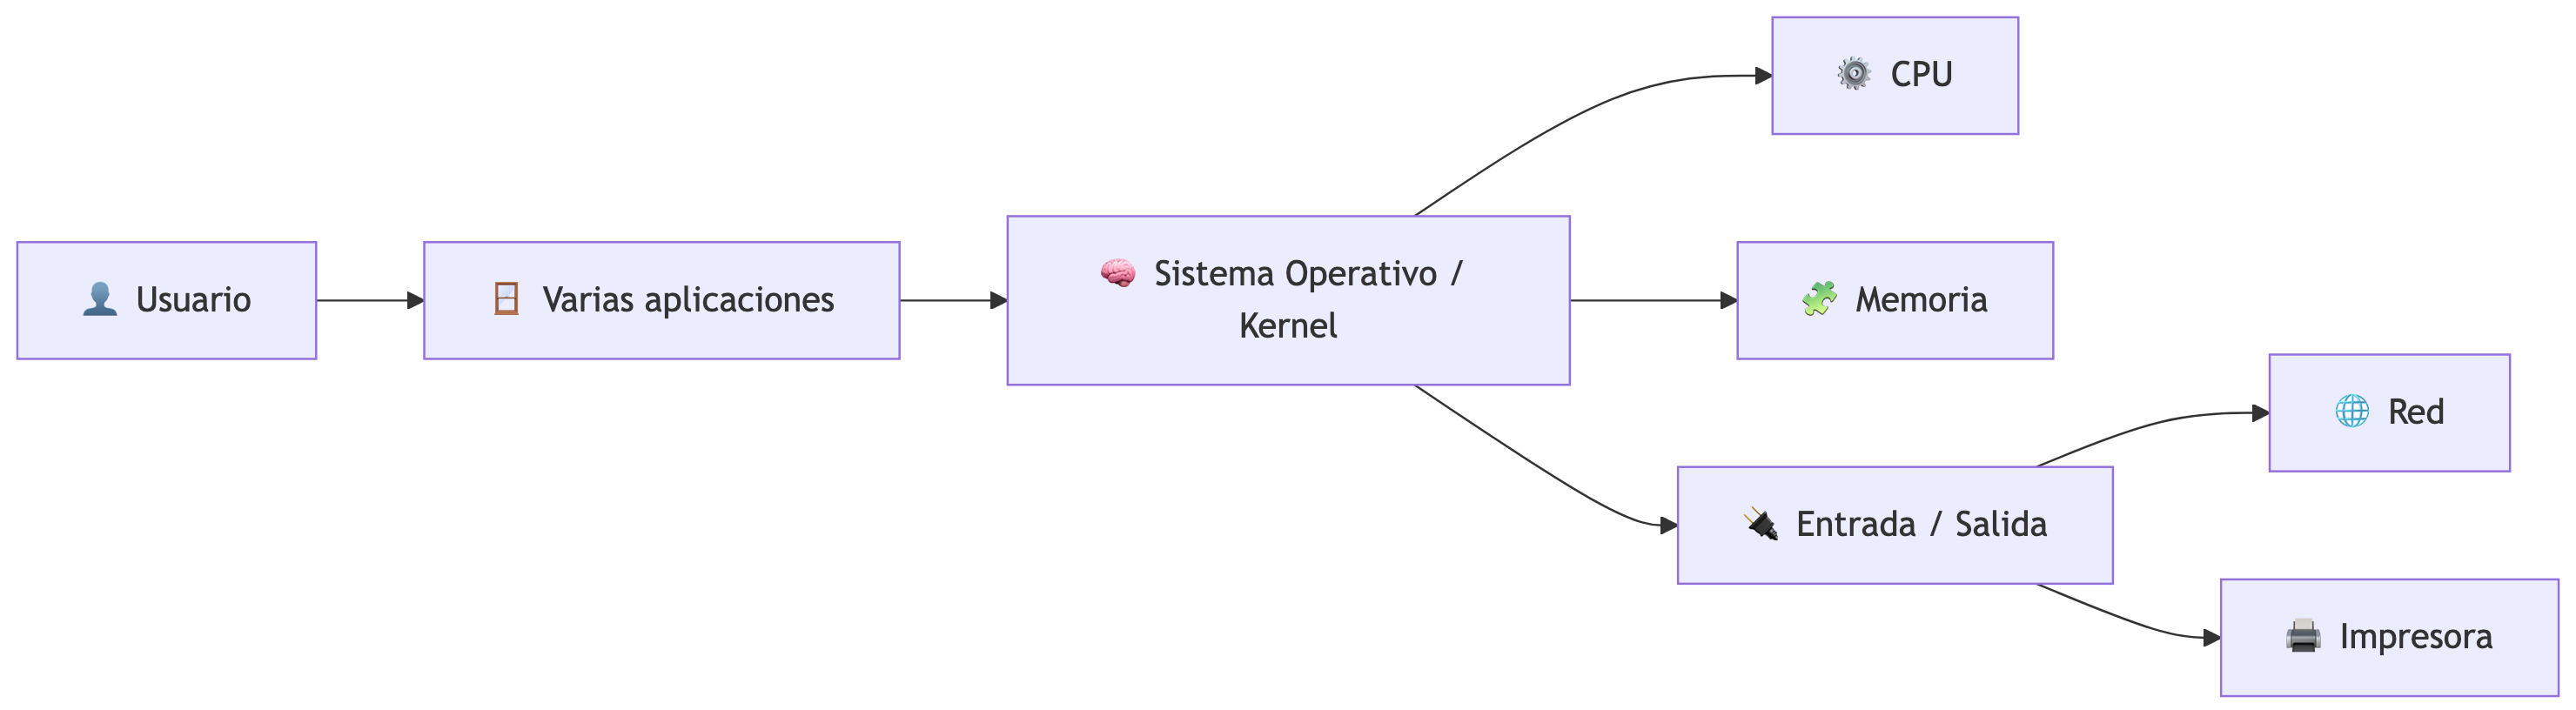
\includegraphics[width=12.41in,height=3.44in]{capitulos/11_actividad_diagnostico_sistema_operativo_respuestas_files/figure-latex/mermaid-figure-1.png}

\bookmarksetup{startatroot}

\chapter{Misión 1. Diagnóstico inicial --- 5
puntos}\label{misiuxf3n-1.-diagnuxf3stico-inicial-5-puntos-1}

\section{1. ¿Cuál parece ser el principal
problema?}\label{cuuxe1l-parece-ser-el-principal-problema}

Una respuesta razonable sería que existe \textbf{alta competencia por
tiempo de CPU}, especialmente por el navegador y el antivirus.

El navegador aparece ejecutándose con \textbf{55 \% de CPU} y el
antivirus requiere otro \textbf{24 \%}. Al mismo tiempo existen varios
procesos en estado \texttt{Ready}, es decir, preparados para ejecutar
pero esperando que el planificador les asigne CPU.

Esto ayuda a explicar por qué el usuario percibe retrasos al cambiar
entre aplicaciones.

\begin{tcolorbox}[enhanced jigsaw, arc=.35mm, bottomrule=.15mm, bottomtitle=1mm, breakable, colback=white, colbacktitle=quarto-callout-note-color!10!white, colframe=quarto-callout-note-color-frame, coltitle=black, left=2mm, leftrule=.75mm, opacityback=0, opacitybacktitle=0.6, rightrule=.15mm, title=\textcolor{quarto-callout-note-color}{\faInfo}\hspace{0.5em}{Pero cuidado}, titlerule=0mm, toprule=.15mm, toptitle=1mm]

Los datos no demuestran que exista un único culpable. Estamos realizando
un diagnóstico con la evidencia disponible. También deben considerarse
memoria, red, almacenamiento y dispositivos de entrada/salida.

\end{tcolorbox}

\section{2. ¿Qué otros factores pueden
contribuir?}\label{quuxe9-otros-factores-pueden-contribuir}

Entre las respuestas justificables están:

\begin{itemize}
\tightlist
\item
  varias aplicaciones abiertas simultáneamente;
\item
  consumo de memoria del navegador y otros programas;
\item
  actividad del antivirus en segundo plano;
\item
  descarga de un archivo grande y utilización de red/almacenamiento;
\item
  reproducción de video y audio;
\item
  espera de la impresora;
\item
  posibles operaciones de entrada/salida;
\item
  cambios frecuentes entre procesos.
\end{itemize}

La memoria reportada para los procesos mostrados suma aproximadamente
\textbf{4 GB}, por lo que no podemos afirmar solamente con esta tabla
que los 8 GB estén agotados. Sin embargo, el Sistema Operativo y otros
procesos no mostrados también utilizan memoria.

\section{3. ¿La CPU está dañada?}\label{la-cpu-estuxe1-dauxf1ada}

No existe evidencia suficiente para concluirlo.

Una computadora puede sentirse lenta aunque el procesador funcione
correctamente. El problema puede encontrarse en la \textbf{carga de
trabajo}, la planificación, la memoria, el almacenamiento, la red, un
dispositivo de E/S o un proceso específico.

\begin{quote}
\textbf{Diagnosticar no significa adivinar el componente dañado;
significa interpretar evidencias.}
\end{quote}

\bookmarksetup{startatroot}

\chapter{Misión 2. ¿Qué ocurre dentro del Sistema Operativo? --- 5
puntos}\label{misiuxf3n-2.-quuxe9-ocurre-dentro-del-sistema-operativo-5-puntos-1}

No era obligatorio mencionar exactamente cuatro componentes específicos.
Lo importante era identificar mecanismos coherentes y explicar su
participación.

{\def\LTcaptype{none} % do not increment counter
\begin{longtable}[]{@{}
  >{\raggedright\arraybackslash}p{(\linewidth - 2\tabcolsep) * \real{0.5000}}
  >{\raggedright\arraybackslash}p{(\linewidth - 2\tabcolsep) * \real{0.5000}}@{}}
\toprule\noalign{}
\begin{minipage}[b]{\linewidth}\raggedright
Componente o mecanismo
\end{minipage} & \begin{minipage}[b]{\linewidth}\raggedright
Papel en el escenario
\end{minipage} \\
\midrule\noalign{}
\endhead
\bottomrule\noalign{}
\endlastfoot
\textbf{Kernel} & Coordina el acceso de los procesos a CPU, memoria y
dispositivos. \\
\textbf{Scheduler} & Decide qué proceso preparado obtiene tiempo de
CPU. \\
\textbf{PCB} & Conserva la información necesaria para administrar cada
proceso y reanudarlo después de una interrupción o espera. \\
\textbf{Dispatcher / cambio de contexto} & Permite entregar la CPU a
otro proceso y continuar posteriormente con el anterior. \\
\textbf{Gestión de memoria} & Controla la memoria utilizada por los
diferentes procesos. \\
\textbf{Drivers y E/S} & Permiten al Sistema Operativo comunicarse con
dispositivos como la impresora. \\
\end{longtable}
}

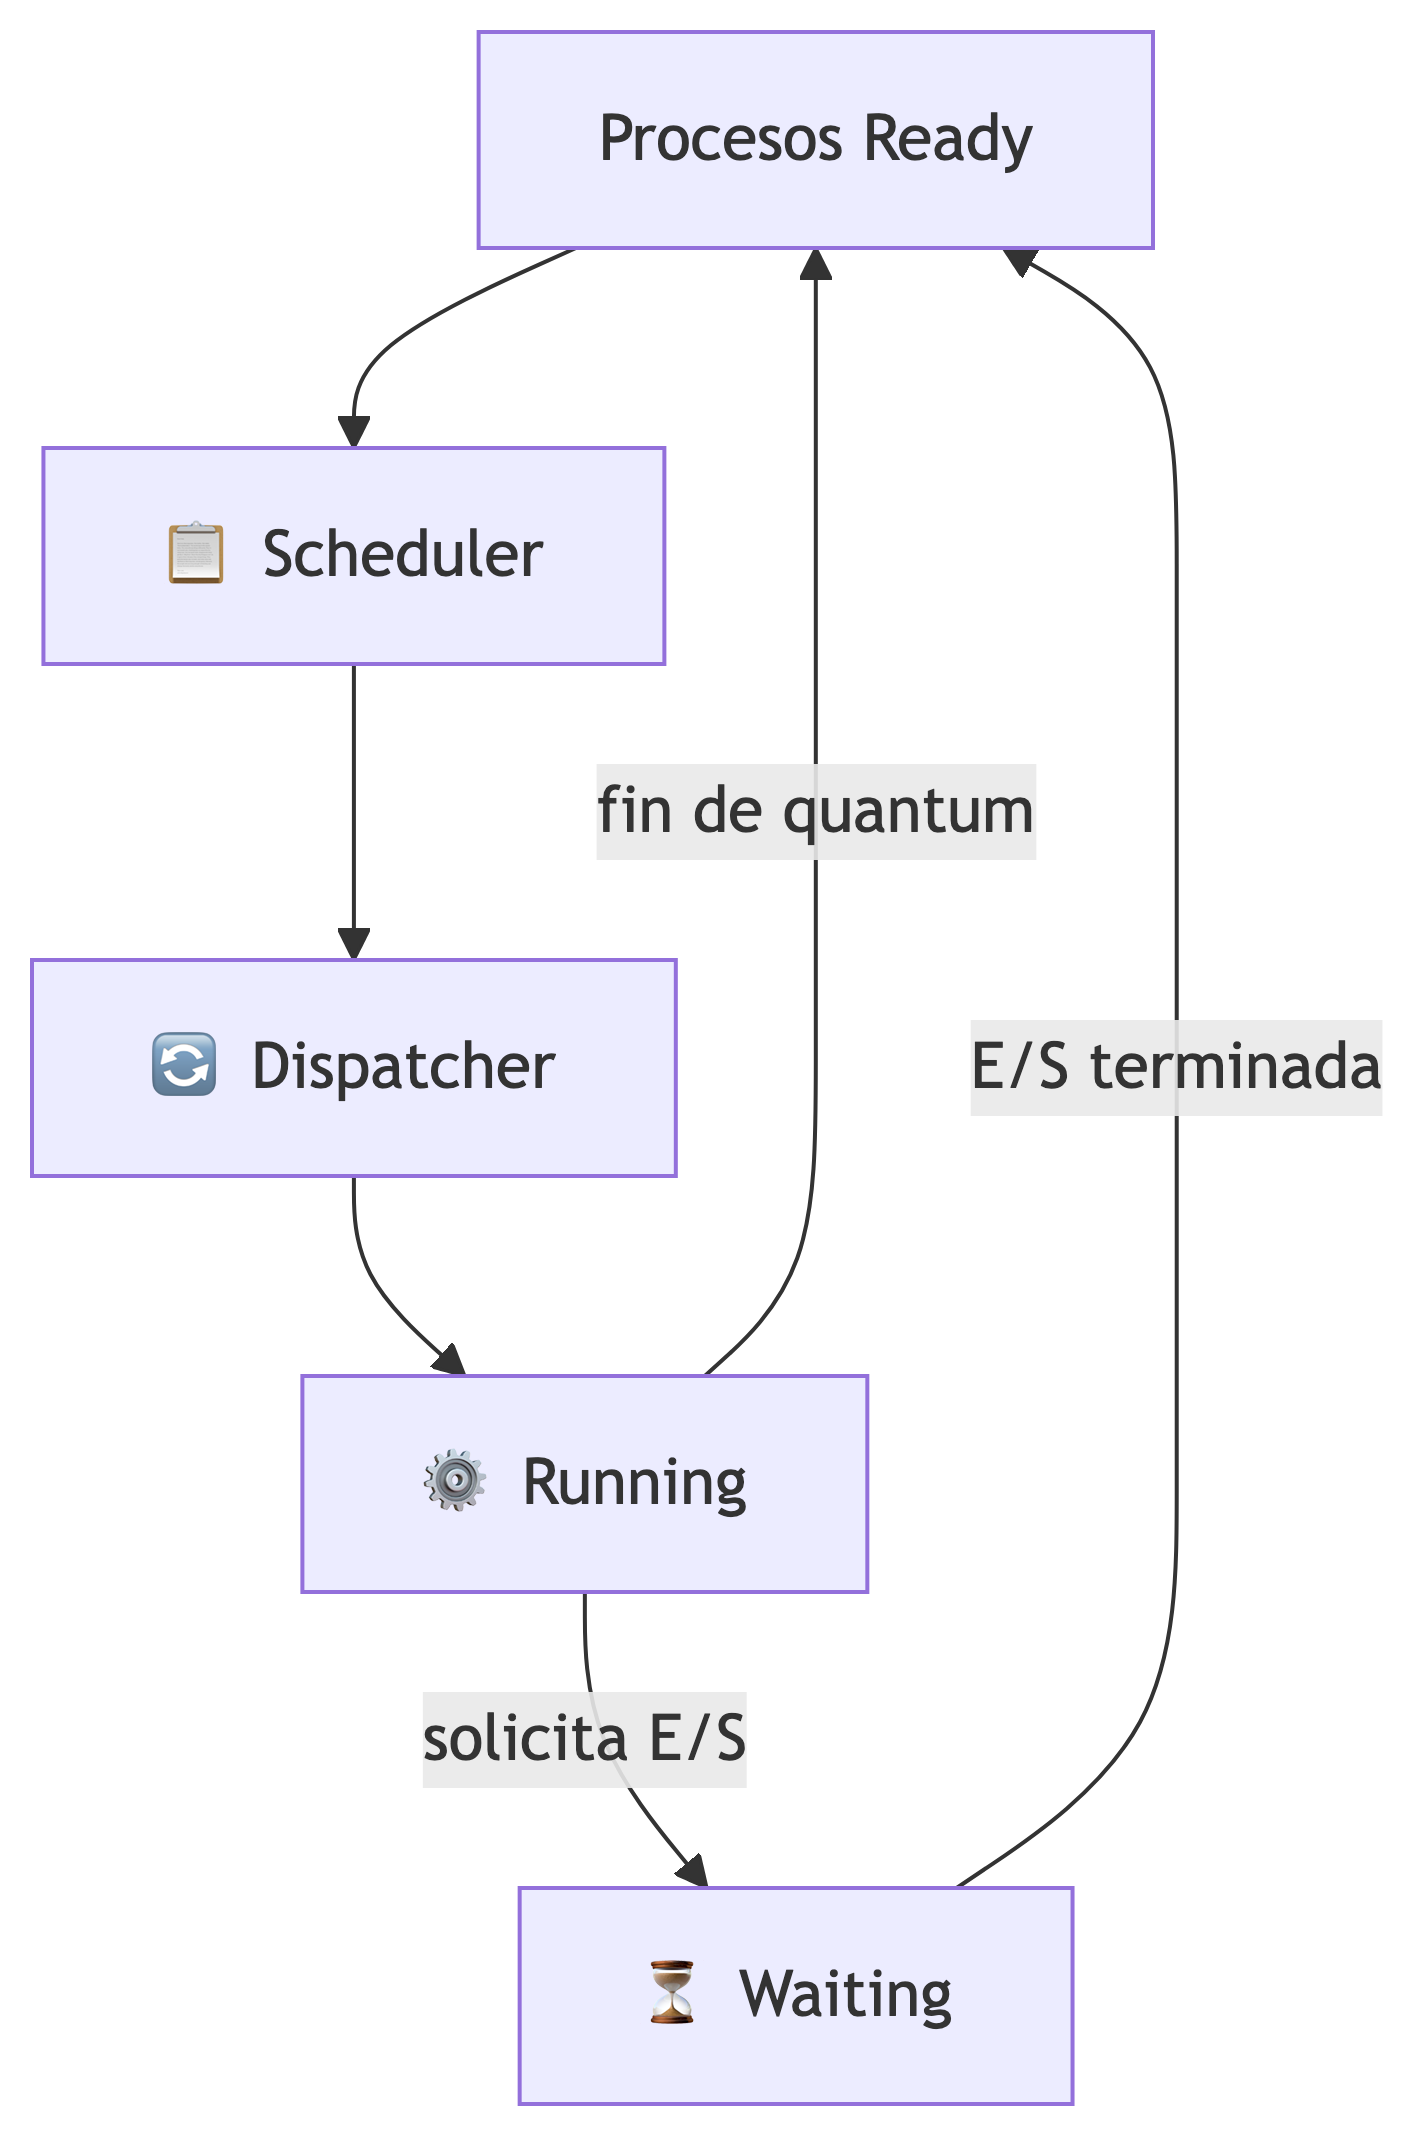
\includegraphics[width=3.68in,height=5.56in]{capitulos/11_actividad_diagnostico_sistema_operativo_respuestas_files/figure-latex/mermaid-figure-6.png}

\begin{tcolorbox}[enhanced jigsaw, arc=.35mm, bottomrule=.15mm, bottomtitle=1mm, breakable, colback=white, colbacktitle=quarto-callout-tip-color!10!white, colframe=quarto-callout-tip-color-frame, coltitle=black, left=2mm, leftrule=.75mm, opacityback=0, opacitybacktitle=0.6, rightrule=.15mm, title=\textcolor{quarto-callout-tip-color}{\faLightbulb}\hspace{0.5em}{Lo que buscábamos comprobar}, titlerule=0mm, toprule=.15mm, toptitle=1mm]

Que pudieran relacionar los conceptos. Por ejemplo: \textbf{Scheduler →
selecciona → Dispatcher → entrega CPU → proceso ejecuta → PCB conserva
el contexto}.

\end{tcolorbox}

\bookmarksetup{startatroot}

\chapter{Misión 3. Sigan el proceso de impresión --- 5
puntos}\label{misiuxf3n-3.-sigan-el-proceso-de-impresiuxf3n-5-puntos}

\section{Una secuencia posible}\label{una-secuencia-posible}

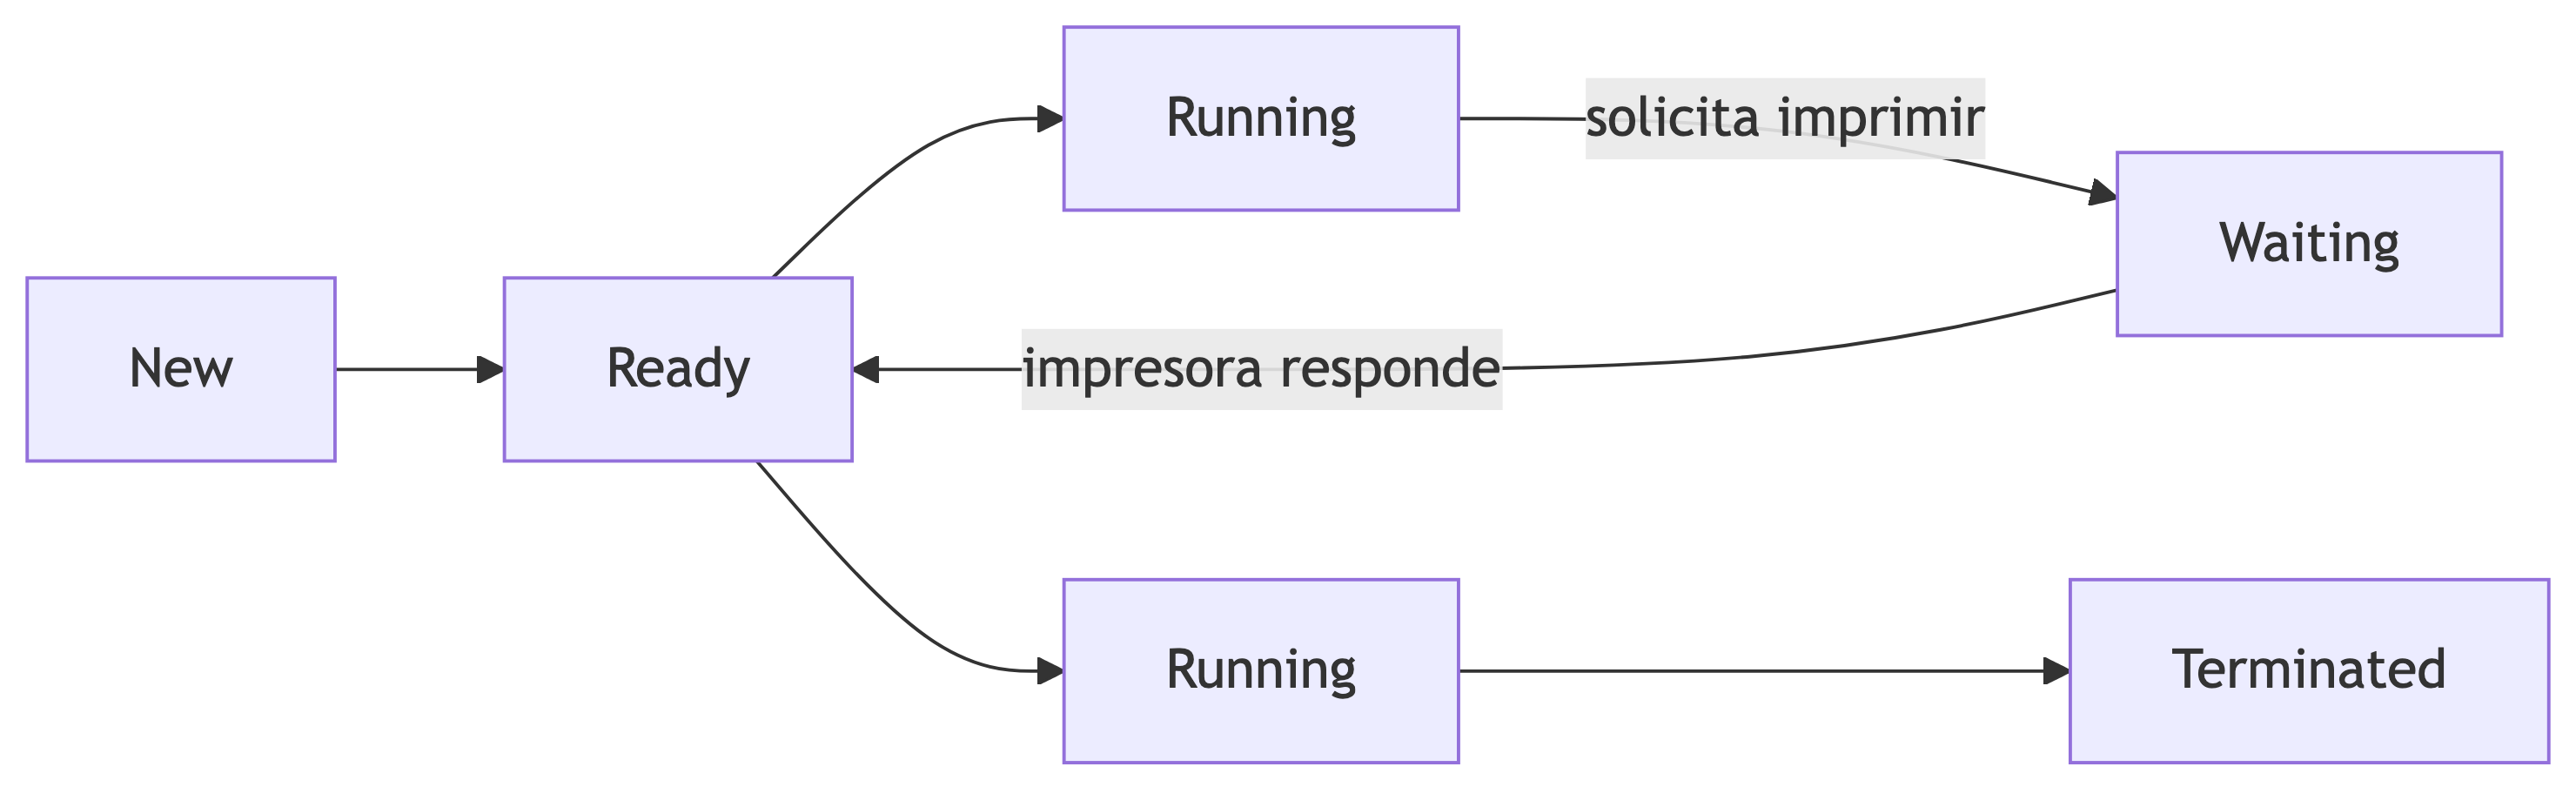
\includegraphics[width=7.92in,height=2.43in]{capitulos/11_actividad_diagnostico_sistema_operativo_respuestas_files/figure-latex/mermaid-figure-5.png}

\section{\texorpdfstring{a. ¿Por qué aparece
\texttt{Waiting}?}{a. ¿Por qué aparece Waiting?}}\label{a.-por-quuxe9-aparece-waiting}

Porque el proceso realizó una operación que depende de un evento
externo: la operación de impresión.

Mientras espera la respuesta correspondiente, no tiene sentido
mantenerlo ocupando la CPU. El Sistema Operativo puede utilizar ese
tiempo para ejecutar otros procesos.

\section{b. ¿Qué debe conservar el Sistema
Operativo?}\label{b.-quuxe9-debe-conservar-el-sistema-operativo}

Debe conservar la información necesaria para poder continuar
posteriormente la ejecución. Esa información se representa
conceptualmente mediante el \textbf{PCB (Process Control Block)}.

Entre otros elementos puede incluir:

\begin{itemize}
\tightlist
\item
  identificador del proceso;
\item
  estado;
\item
  contador de programa;
\item
  registros;
\item
  información de planificación;
\item
  información relacionada con memoria;
\item
  recursos y archivos asociados.
\end{itemize}

La idea central no era memorizar toda la lista, sino comprender que
\textbf{el proceso debe poder detenerse y continuar sin comenzar desde
cero}.

\section{c.~¿Qué ocurre cuando responde la
impresora?}\label{c.-quuxe9-ocurre-cuando-responde-la-impresora}

Una secuencia razonable es:

\textbf{Waiting → Ready → Running}

La finalización del evento de E/S permite que el proceso deje de estar
bloqueado. Sin embargo, esto \textbf{no significa necesariamente que
pase inmediatamente a Running}: primero queda disponible
(\texttt{Ready}) y el Scheduler decidirá cuándo vuelve a utilizar CPU.

\bookmarksetup{startatroot}

\chapter{Misión 4. Ustedes son el Sistema Operativo --- 5
puntos}\label{misiuxf3n-4.-ustedes-son-el-sistema-operativo-5-puntos-1}

Los procesos eran:

{\def\LTcaptype{none} % do not increment counter
\begin{longtable}[]{@{}lrrl@{}}
\toprule\noalign{}
Proceso & CPU & Prioridad & Tipo \\
\midrule\noalign{}
\endhead
\bottomrule\noalign{}
\endlastfoot
P1 & 8 ms & 3 & Navegador interactivo \\
P2 & 2 ms & 1 & Proceso crítico del sistema \\
P3 & 6 ms & 2 & Antivirus \\
P4 & 3 ms & 3 & Reproductor multimedia \\
\end{longtable}
}

\section{1. ¿Qué criterio utilizar?}\label{quuxe9-criterio-utilizar}

Aquí \textbf{no buscábamos una única palabra}.

Una respuesta bien argumentada puede proponer \textbf{planificación por
prioridades} para favorecer P2, combinada con reparto de CPU para
conservar la respuesta de los procesos interactivos.

También era razonable mencionar \textbf{Round Robin} para los procesos
interactivos, porque evita que uno conserve indefinidamente el
procesador.

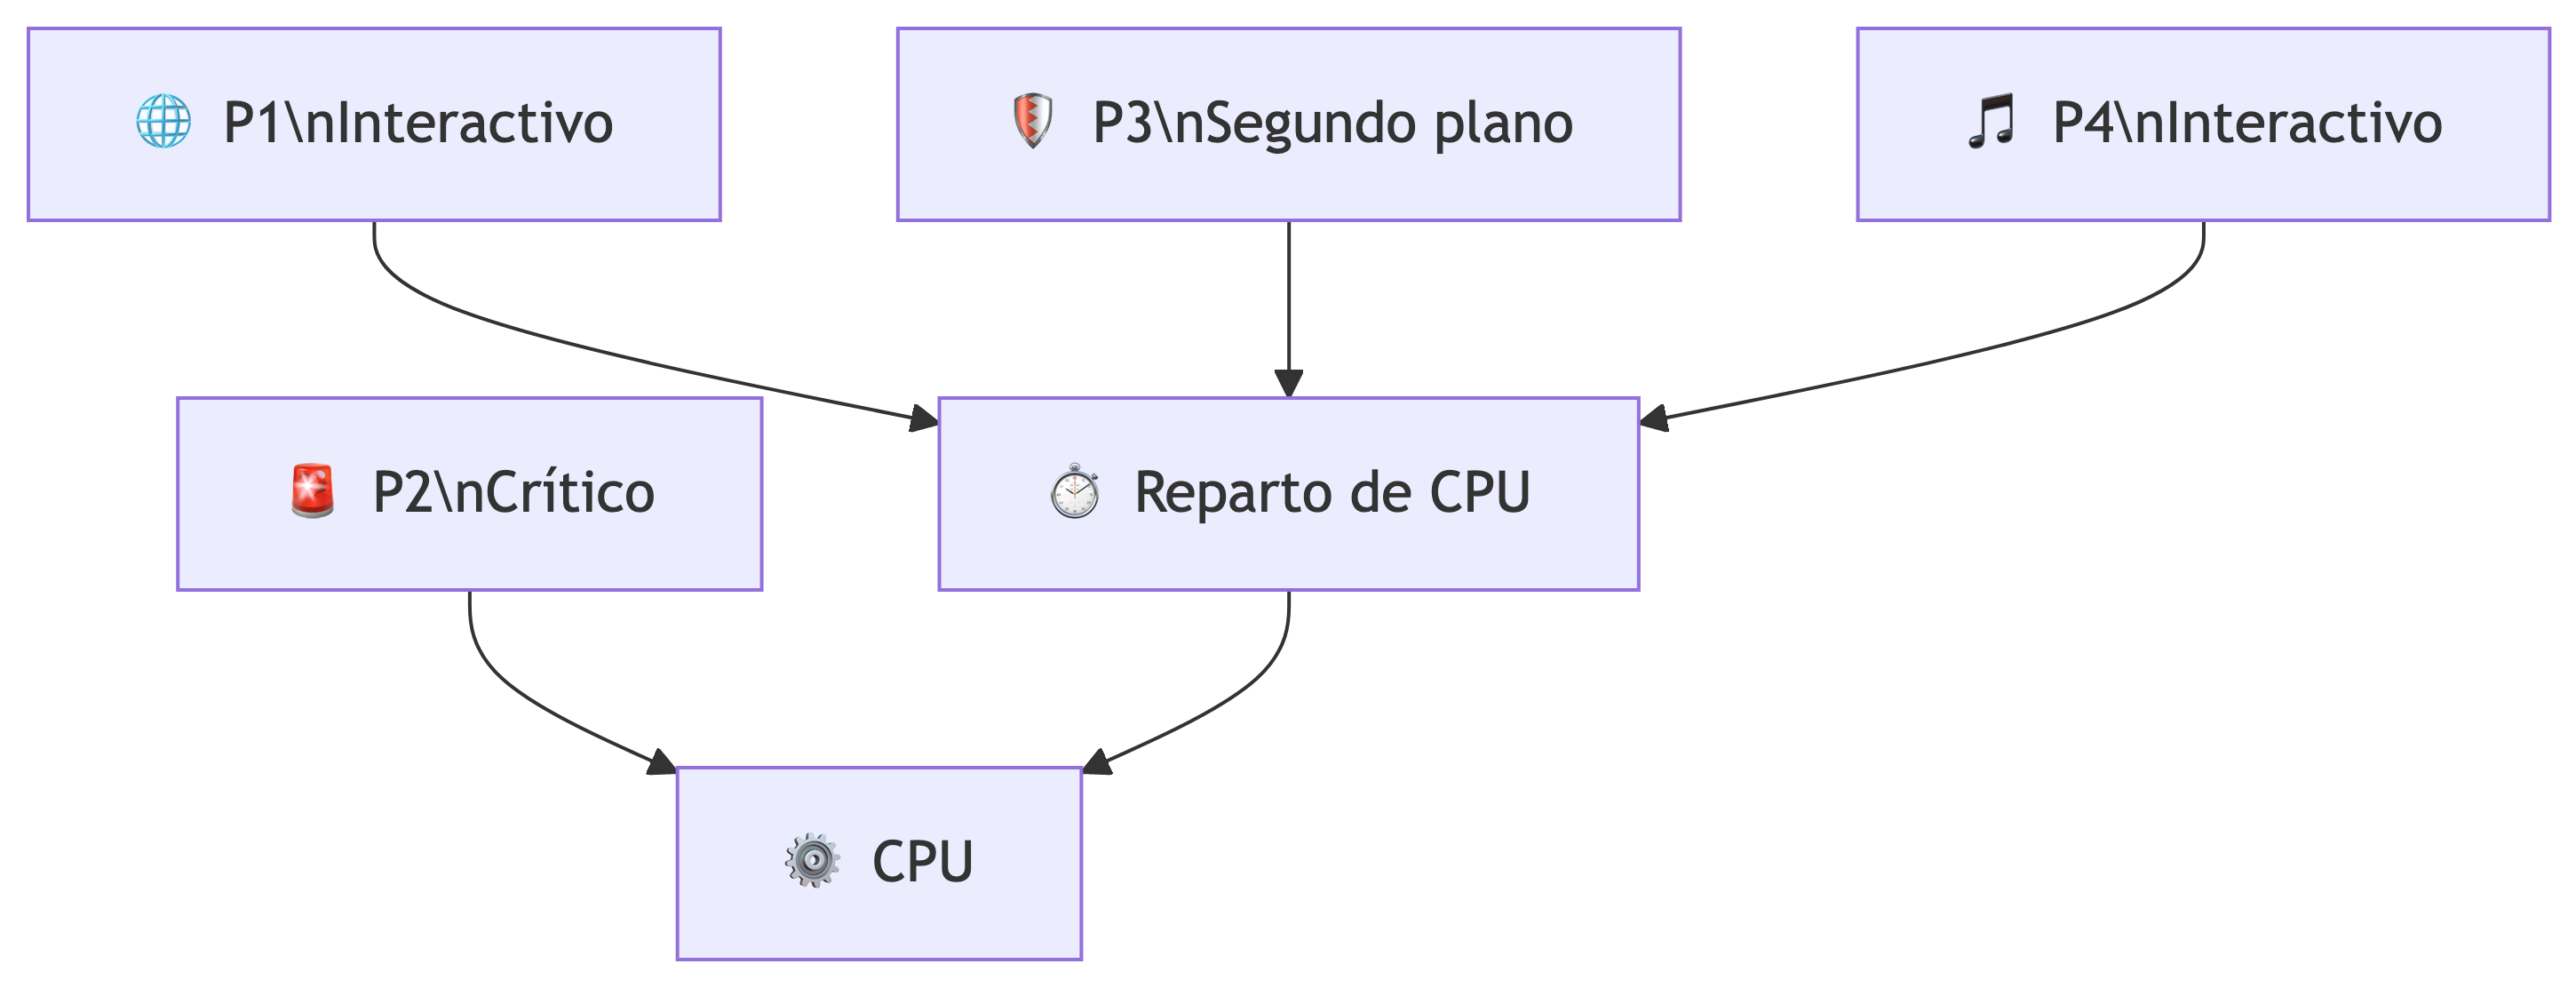
\includegraphics[width=7.56in,height=2.9in]{capitulos/11_actividad_diagnostico_sistema_operativo_respuestas_files/figure-latex/mermaid-figure-4.png}

\begin{tcolorbox}[enhanced jigsaw, arc=.35mm, bottomrule=.15mm, bottomtitle=1mm, breakable, colback=white, colbacktitle=quarto-callout-warning-color!10!white, colframe=quarto-callout-warning-color-frame, coltitle=black, left=2mm, leftrule=.75mm, opacityback=0, opacitybacktitle=0.6, rightrule=.15mm, title=\textcolor{quarto-callout-warning-color}{\faExclamationTriangle}\hspace{0.5em}{No confundir}, titlerule=0mm, toprule=.15mm, toptitle=1mm]

SJF podría reducir el tiempo promedio de espera en ciertos escenarios,
pero seleccionar siempre el proceso más corto no considera por sí mismo
que \textbf{P2 es crítico} ni garantiza el comportamiento deseado para
aplicaciones interactivas.

\end{tcolorbox}

\section{2. ¿Todos deben tratarse
igual?}\label{todos-deben-tratarse-igual}

No necesariamente.

P2 representa una tarea crítica del sistema, mientras P1 y P4 son
interactivos y P3 corresponde a una tarea en segundo plano.

El Sistema Operativo puede necesitar equilibrar:

\begin{itemize}
\tightlist
\item
  prioridad;
\item
  capacidad de respuesta;
\item
  equidad;
\item
  utilización del procesador.
\end{itemize}

\section{3. ¿Qué pasa si uno conserva demasiado la
CPU?}\label{quuxe9-pasa-si-uno-conserva-demasiado-la-cpu}

Los demás procesos pueden permanecer demasiado tiempo esperando.

El usuario percibiría aplicaciones congeladas o poco responsivas.
Precisamente por eso los sistemas multitarea necesitan mecanismos de
planificación y, según la política utilizada, \textbf{preempción y
quantum de tiempo}.

\bookmarksetup{startatroot}

\chapter{Misión 5. Diagnóstico final --- 5
puntos}\label{misiuxf3n-5.-diagnuxf3stico-final-5-puntos-1}

\section{A. ¿Qué ocurre cuando presionamos
Imprimir?}\label{a.-quuxe9-ocurre-cuando-presionamos-imprimir}

Una representación simplificada sería:

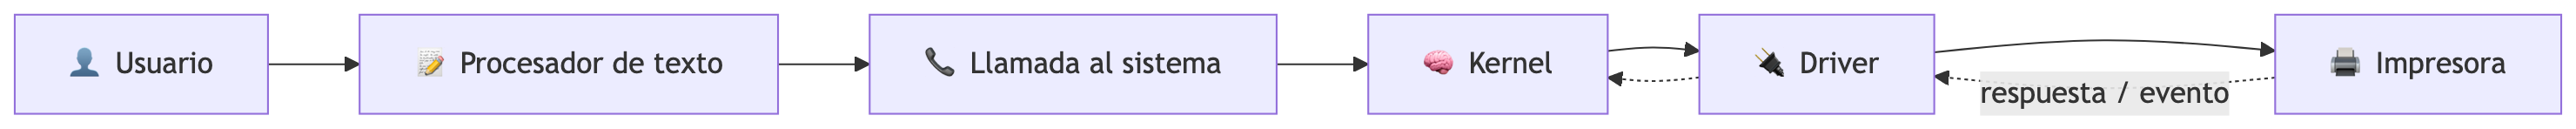
\includegraphics[width=14.64in,height=0.74in]{capitulos/11_actividad_diagnostico_sistema_operativo_respuestas_files/figure-latex/mermaid-figure-3.png}

El usuario no controla directamente la impresora.

\begin{enumerate}
\def\labelenumi{\arabic{enumi}.}
\tightlist
\item
  El usuario solicita imprimir desde la aplicación.
\item
  La aplicación solicita un servicio al Sistema Operativo.
\item
  El Kernel coordina la operación.
\item
  El controlador o \textbf{driver} permite la comunicación con el
  dispositivo.
\item
  La impresora realiza la operación.
\item
  Mientras se espera el evento de E/S, el proceso relacionado puede
  quedar bloqueado.
\item
  Cuando la operación permite continuar, el proceso puede regresar a
  \texttt{Ready}.
\end{enumerate}

\section{B. ¿Qué acciones podrían
realizarse?}\label{b.-quuxe9-acciones-podruxedan-realizarse}

Una respuesta prudente sería \textbf{observar antes de cerrar procesos
al azar}.

Podrían:

\begin{enumerate}
\def\labelenumi{\arabic{enumi}.}
\tightlist
\item
  revisar qué proceso consume más CPU;
\item
  observar si el consumo elevado se mantiene;
\item
  verificar presión de memoria;
\item
  revisar actividad de disco, red y dispositivos;
\item
  comprobar el estado de la impresión;
\item
  pausar o reprogramar tareas de segundo plano si están afectando el
  trabajo interactivo;
\item
  cerrar únicamente aplicaciones o pestañas que no sean necesarias.
\end{enumerate}

\subsection{¿Qué observar primero?}\label{quuxe9-observar-primero}

Con los datos proporcionados, comenzar por \textbf{CPU y procesos
activos} es razonable porque el navegador y el antivirus muestran una
carga importante y existen varios procesos en \texttt{Ready}.

Después habría que revisar memoria y E/S para confirmar o descartar
otros cuellos de botella.

\bookmarksetup{startatroot}

\chapter{Uniendo todo}\label{uniendo-todo}

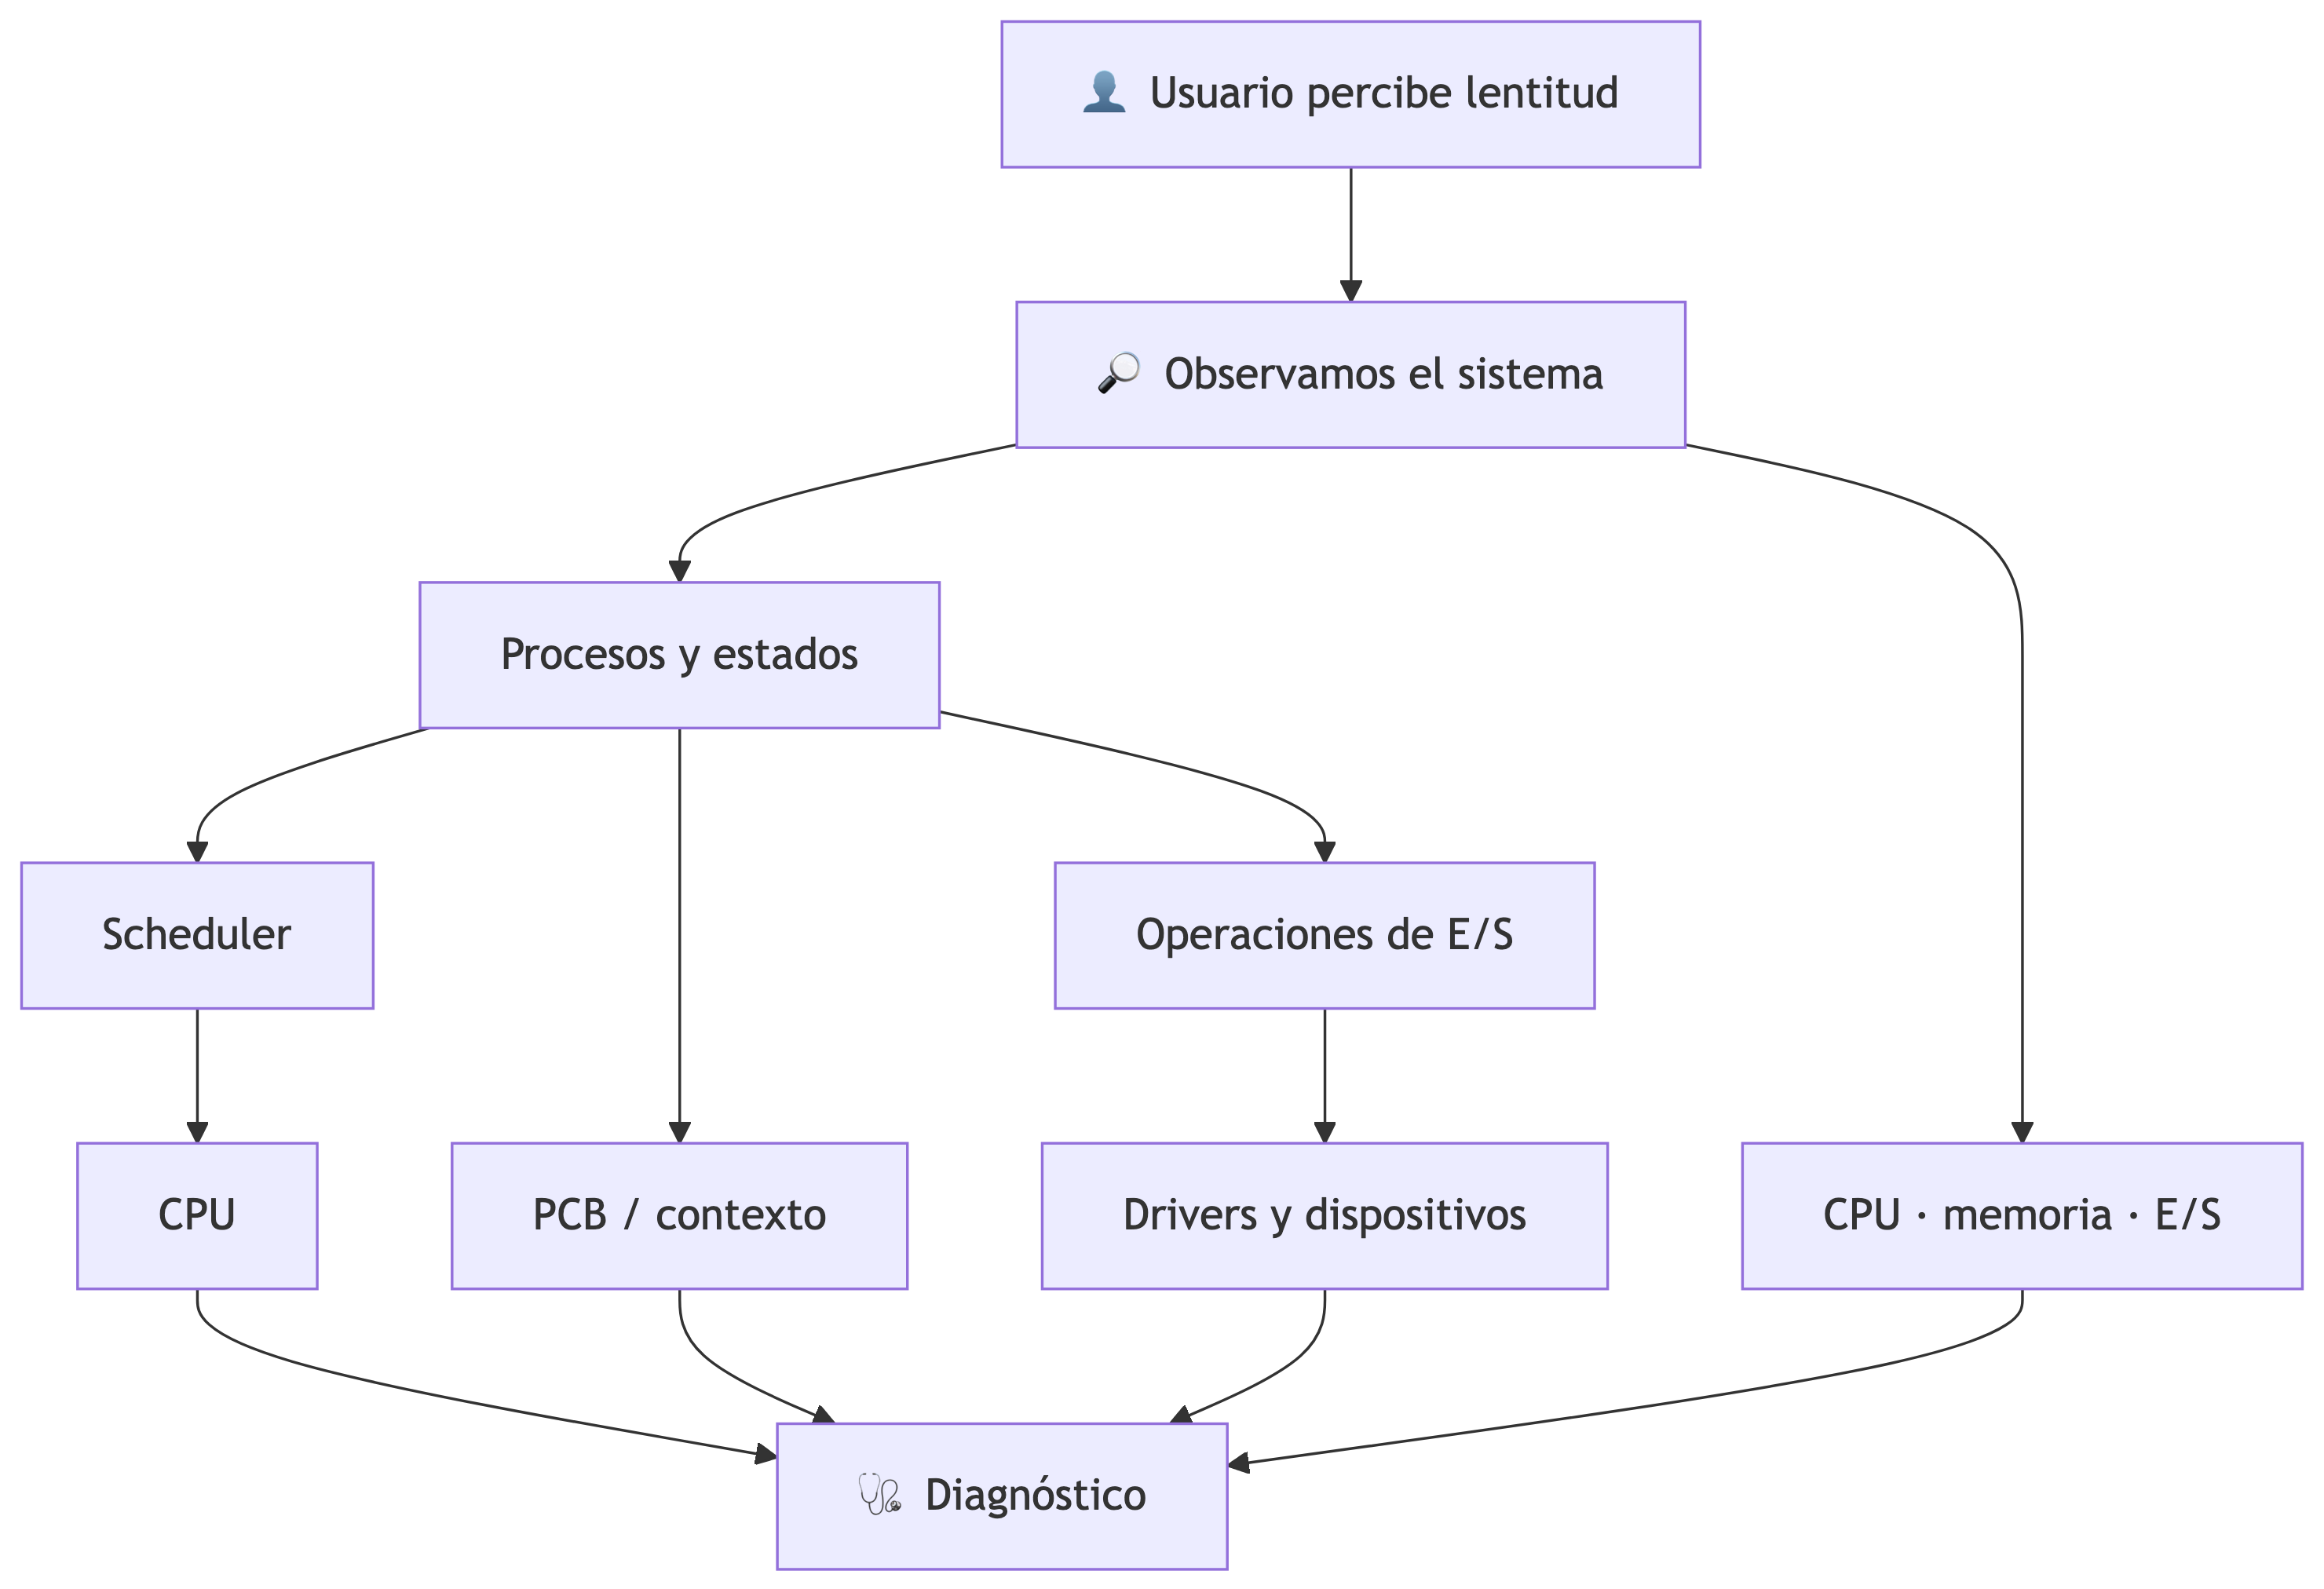
\includegraphics[width=8.98in,height=6.15in]{capitulos/11_actividad_diagnostico_sistema_operativo_respuestas_files/figure-latex/mermaid-figure-2.png}

\begin{tcolorbox}[enhanced jigsaw, arc=.35mm, bottomrule=.15mm, bottomtitle=1mm, breakable, colback=white, colbacktitle=quarto-callout-important-color!10!white, colframe=quarto-callout-important-color-frame, coltitle=black, left=2mm, leftrule=.75mm, opacityback=0, opacitybacktitle=0.6, rightrule=.15mm, title=\textcolor{quarto-callout-important-color}{\faExclamation}\hspace{0.5em}{La respuesta más importante de toda la actividad}, titlerule=0mm, toprule=.15mm, toptitle=1mm]

Un buen diagnóstico de Sistemas Operativos \textbf{no consiste en
encontrar rápidamente un culpable}. Consiste en observar procesos,
estados, recursos y eventos; relacionarlos con el funcionamiento del
Kernel; formular una explicación y comprobar si la evidencia la
respalda.

\end{tcolorbox}

\bookmarksetup{startatroot}

\chapter{¿Cómo podía obtenerse el
punteo?}\label{cuxf3mo-poduxeda-obtenerse-el-punteo}

{\def\LTcaptype{none} % do not increment counter
\begin{longtable}[]{@{}
  >{\raggedright\arraybackslash}p{(\linewidth - 2\tabcolsep) * \real{0.5000}}
  >{\raggedright\arraybackslash}p{(\linewidth - 2\tabcolsep) * \real{0.5000}}@{}}
\toprule\noalign{}
\begin{minipage}[b]{\linewidth}\raggedright
Área evaluada
\end{minipage} & \begin{minipage}[b]{\linewidth}\raggedright
5 puntos cuando\ldots{}
\end{minipage} \\
\midrule\noalign{}
\endhead
\bottomrule\noalign{}
\endlastfoot
Diagnóstico & Utiliza los datos del escenario y evita conclusiones sin
evidencia. \\
Componentes del SO & Identifica componentes correctos y explica su
relación con el caso. \\
Procesos y PCB & Interpreta correctamente \texttt{Running},
\texttt{Ready}, \texttt{Waiting} y la conservación del contexto. \\
Planificación & Propone un criterio coherente y lo justifica según el
tipo de proceso. \\
Integración & Relaciona aplicación, Kernel, llamadas al sistema,
drivers, hardware y propone acciones razonables. \\
\end{longtable}
}

\bookmarksetup{startatroot}

\chapter{Para cerrar}\label{para-cerrar}

Si algunas respuestas de tu grupo fueron diferentes de esta guía,
pregúntate:

\begin{itemize}
\tightlist
\item
  ¿Nuestra respuesta estaba sustentada por los datos?
\item
  ¿Utilizamos correctamente los conceptos?
\item
  ¿Podíamos explicar por qué llegamos a esa conclusión?
\item
  ¿Cambiaríamos algo después de escuchar a los demás grupos?
\end{itemize}

\begin{tcolorbox}[enhanced jigsaw, arc=.35mm, bottomrule=.15mm, bottomtitle=1mm, breakable, colback=white, colbacktitle=quarto-callout-tip-color!10!white, colframe=quarto-callout-tip-color-frame, coltitle=black, left=2mm, leftrule=.75mm, opacityback=0, opacitybacktitle=0.6, rightrule=.15mm, title=\textcolor{quarto-callout-tip-color}{\faLightbulb}\hspace{0.5em}{Consejo del Ingeniero}, titlerule=0mm, toprule=.15mm, toptitle=1mm]

En Sistemas Operativos, aprender los nombres de los componentes es
apenas el comienzo.

\textbf{El verdadero aprendizaje aparece cuando puedes explicar qué
están haciendo y por qué.}

\end{tcolorbox}

\bookmarksetup{startatroot}

\chapter{Capítulo 12. Virtualización de Sistemas
Operativos}\label{capuxedtulo-12.-virtualizaciuxf3n-de-sistemas-operativos}

\bookmarksetup{startatroot}

\chapter{Capítulo 12. Virtualización de Sistemas
Operativos}\label{capuxedtulo-12.-virtualizaciuxf3n-de-sistemas-operativos-1}

\section{De una computadora\ldots{} a varias
computadoras}\label{de-una-computadora-a-varias-computadoras}

Hasta ahora hemos estudiado cómo el Sistema Operativo administra
procesos, recursos, hardware e interbloqueos. Ahora utilizaremos esos
conocimientos para comprender una tecnología que permite ejecutar
\textbf{varios sistemas operativos sobre un mismo equipo físico}.

Imaginemos una computadora con:

\begin{itemize}
\tightlist
\item
  procesador;
\item
  16 GB de memoria RAM;
\item
  512 GB de almacenamiento;
\item
  conexión de red;
\item
  Windows, macOS o Linux como sistema principal.
\end{itemize}

La pregunta es:

\begin{quote}
\textbf{¿Podemos utilizar parte de esos recursos para construir otra
computadora sin comprar otro equipo físico?}
\end{quote}

Sí. Esa es precisamente una de las ideas fundamentales de la
\textbf{virtualización}.

\begin{tcolorbox}[enhanced jigsaw, arc=.35mm, bottomrule=.15mm, bottomtitle=1mm, breakable, colback=white, colbacktitle=quarto-callout-tip-color!10!white, colframe=quarto-callout-tip-color-frame, coltitle=black, left=2mm, leftrule=.75mm, opacityback=0, opacitybacktitle=0.6, rightrule=.15mm, title=\textcolor{quarto-callout-tip-color}{\faLightbulb}\hspace{0.5em}{Idea central}, titlerule=0mm, toprule=.15mm, toptitle=1mm]

Una máquina virtual se comporta como una computadora independiente, pero
utiliza recursos proporcionados por una computadora física.

\end{tcolorbox}

\begin{figure}[H]

{\centering 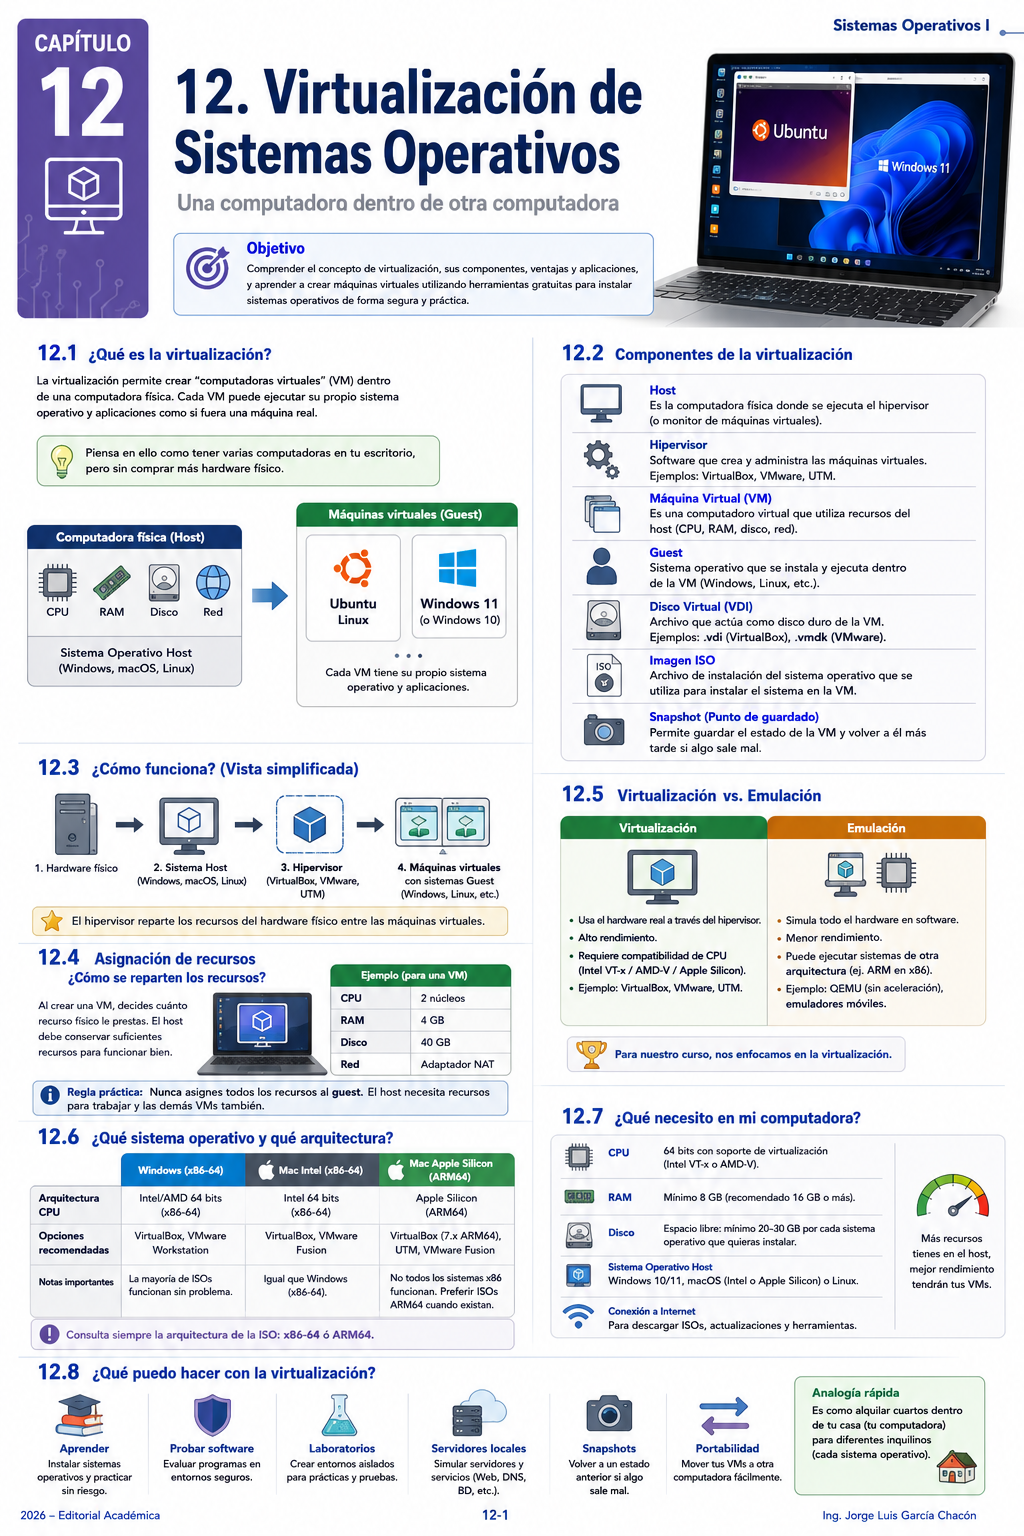
\includegraphics[width=0.92\linewidth,height=\textheight,keepaspectratio]{capitulos/img/capitulo12/virtualizacion_panorama.png}

}

\caption{Panorama visual de la virtualización: una computadora física
puede alojar varias máquinas virtuales.}

\end{figure}%

\begin{center}\rule{0.5\linewidth}{0.5pt}\end{center}

\bookmarksetup{startatroot}

\chapter{Objetivos de aprendizaje}\label{objetivos-de-aprendizaje-8}

Al finalizar este capítulo, el estudiante será capaz de:

\begin{itemize}
\tightlist
\item
  Explicar qué es la virtualización y por qué se utiliza.
\item
  Diferenciar \textbf{host}, \textbf{guest}, \textbf{máquina virtual} e
  \textbf{hipervisor}.
\item
  Comprender cómo CPU, RAM, almacenamiento y red físicos se presentan
  como recursos virtuales.
\item
  Diferenciar \textbf{virtualización} de \textbf{emulación}.
\item
  Reconocer la importancia de la arquitectura \textbf{x86-64} y
  \textbf{ARM64}.
\item
  Identificar alternativas gratuitas actuales para Windows y macOS.
\item
  Seleccionar una herramienta de virtualización de acuerdo con el equipo
  disponible.
\item
  Comprender qué es una imagen ISO, un disco virtual y un snapshot.
\item
  Diseñar la configuración básica de una máquina virtual antes de
  instalarla.
\end{itemize}

\begin{center}\rule{0.5\linewidth}{0.5pt}\end{center}

\bookmarksetup{startatroot}

\chapter{1. ¿Qué es la
virtualización?}\label{quuxe9-es-la-virtualizaciuxf3n}

La \textbf{virtualización} permite crear una representación lógica de
recursos informáticos físicos.

En lugar de que un único Sistema Operativo utilice directamente todos
los recursos del equipo, un software de virtualización puede
proporcionar recursos a una o varias \textbf{máquinas virtuales (VM)}.

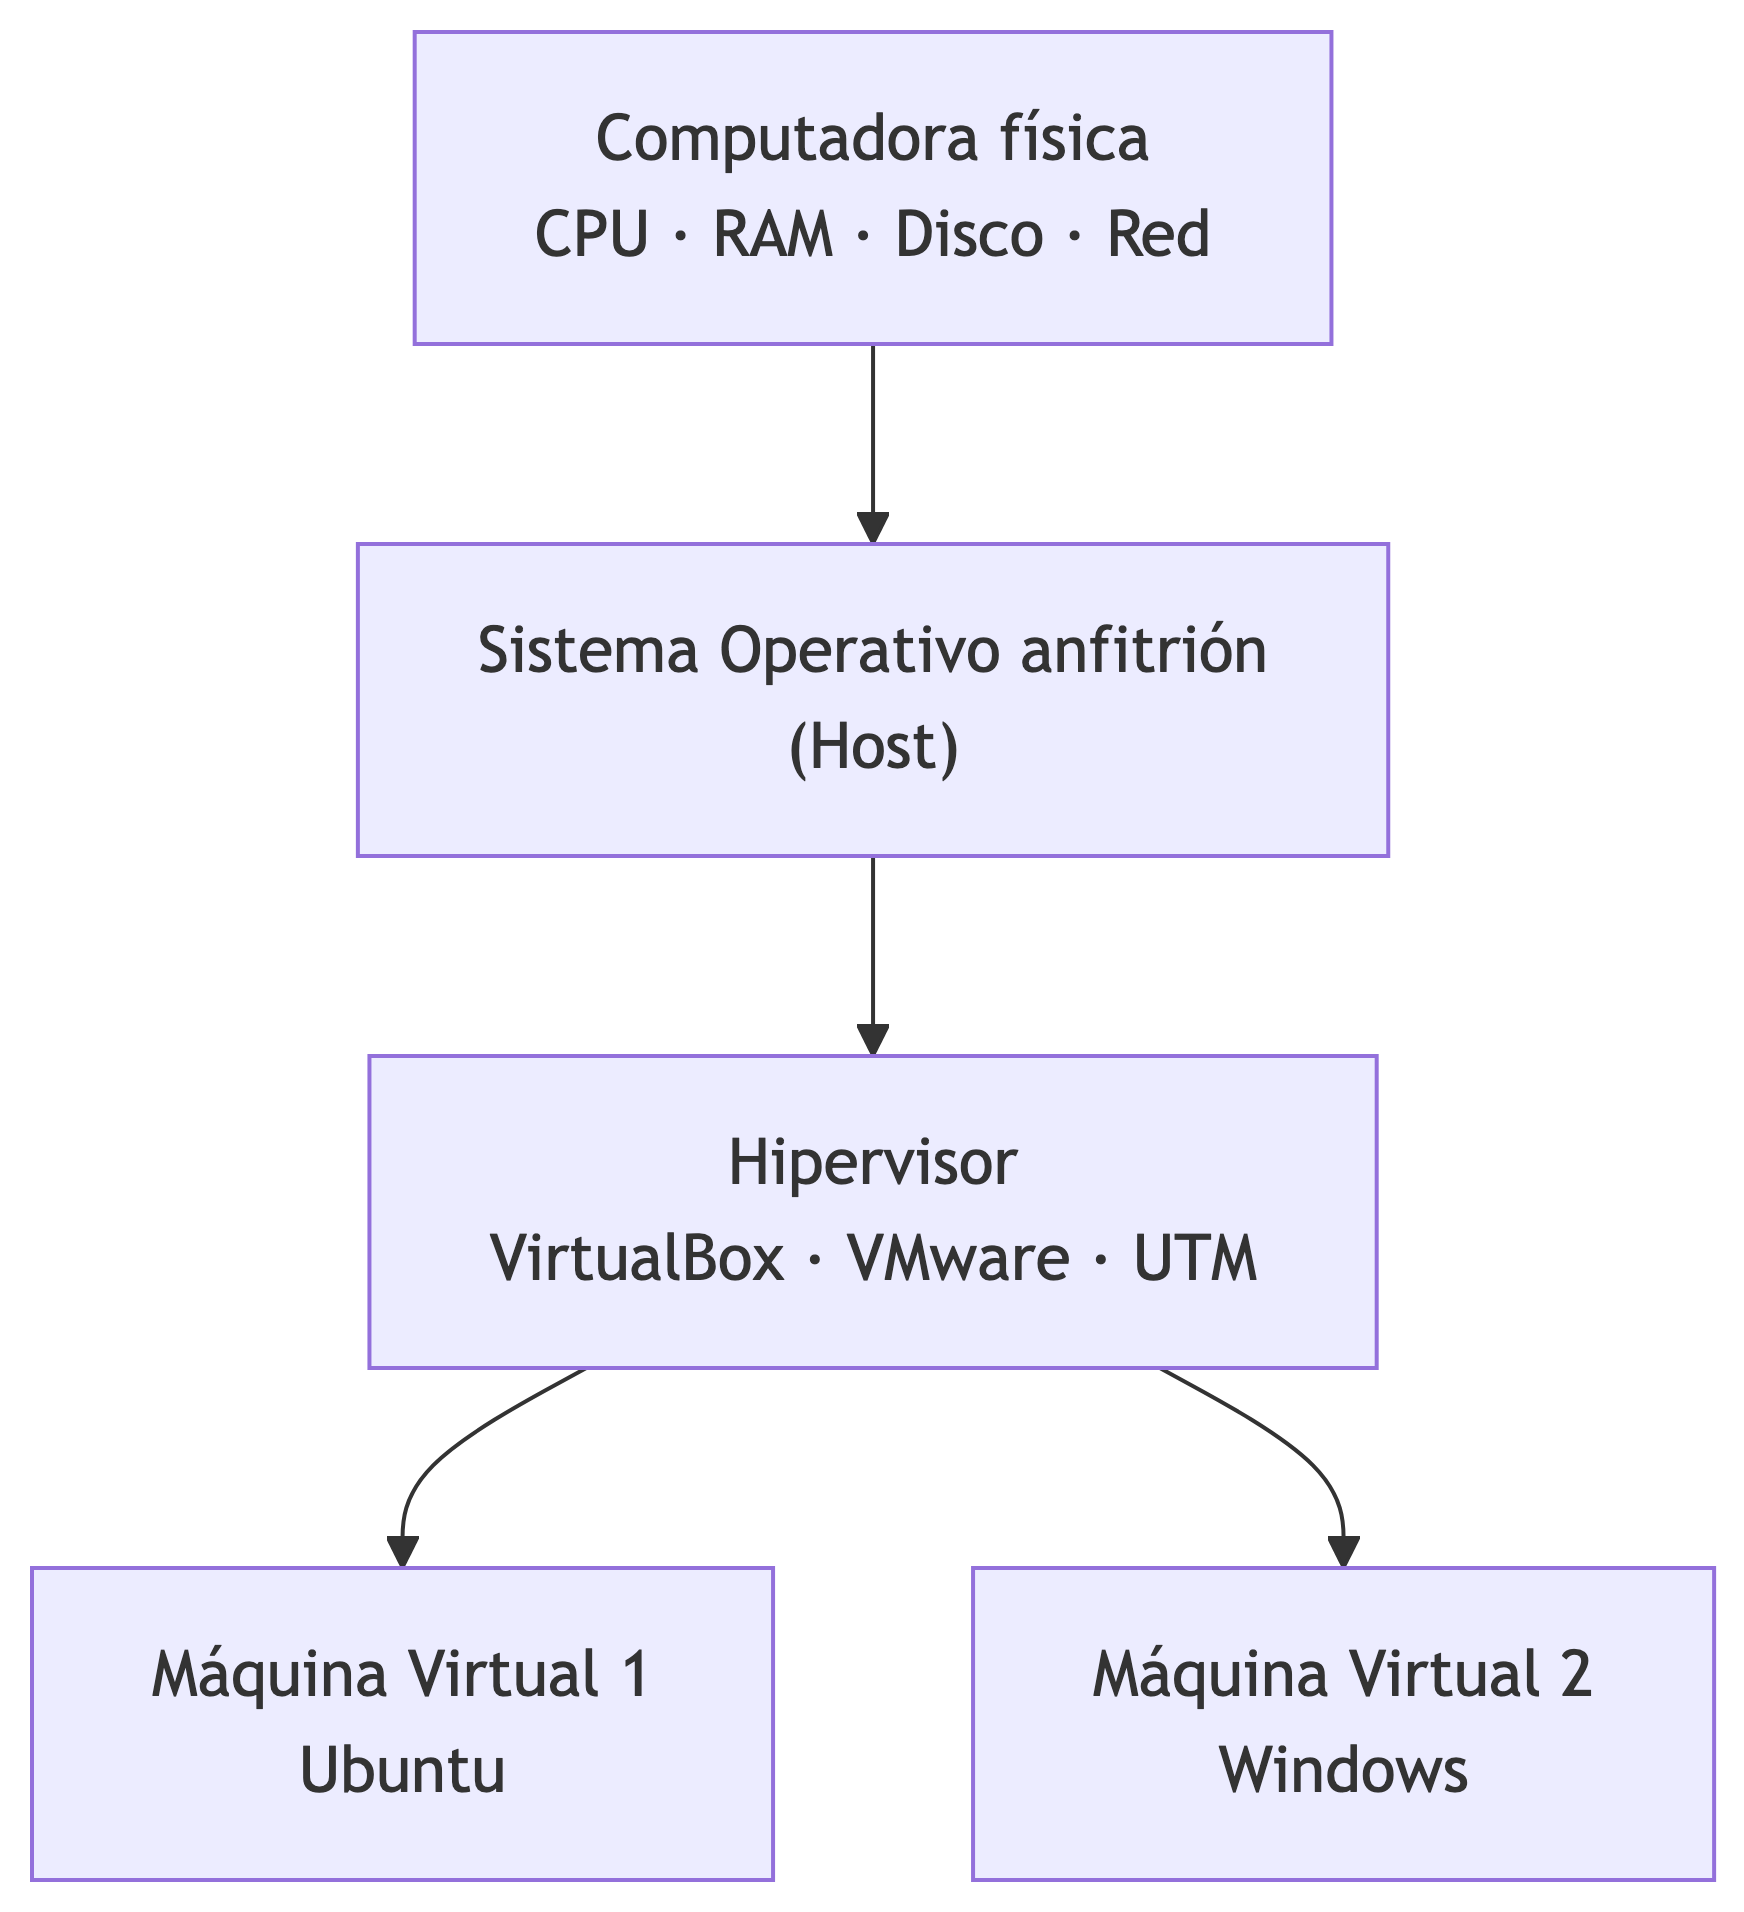
\includegraphics[width=7.2in,height=5.4in]{capitulos/12_virtualizacion_sistemas_operativos_files/figure-latex/mermaid-figure-1.png}

\begin{figure}[H]

{\centering 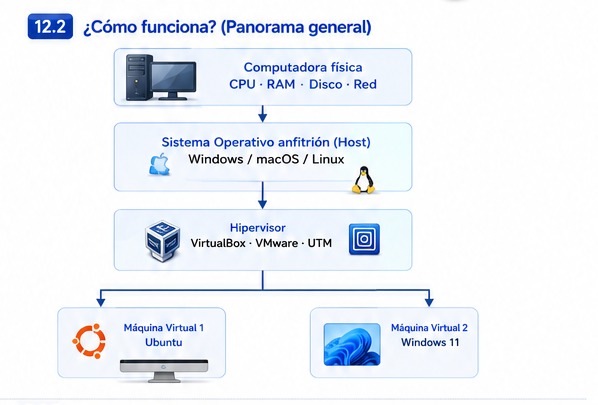
\includegraphics[width=0.88\linewidth,height=\textheight,keepaspectratio]{capitulos/img/capitulo12/virtualizacion_componentes.png}

}

\caption{Relación entre hardware físico, host, hipervisor y máquinas
virtuales.}

\end{figure}%

\begin{tcolorbox}[enhanced jigsaw, arc=.35mm, bottomrule=.15mm, bottomtitle=1mm, breakable, colback=white, colbacktitle=quarto-callout-note-color!10!white, colframe=quarto-callout-note-color-frame, coltitle=black, left=2mm, leftrule=.75mm, opacityback=0, opacitybacktitle=0.6, rightrule=.15mm, title=\textcolor{quarto-callout-note-color}{\faInfo}\hspace{0.5em}{Primera analogía}, titlerule=0mm, toprule=.15mm, toptitle=1mm]

Pensemos en un edificio.

El \textbf{hardware físico} es el edificio completo. El hipervisor
divide y administra espacios. Cada \textbf{máquina virtual} es como un
apartamento: tiene sus propios recursos y puede funcionar de manera
relativamente independiente, aunque todos comparten la misma
infraestructura física.

\end{tcolorbox}

\begin{center}\rule{0.5\linewidth}{0.5pt}\end{center}

\bookmarksetup{startatroot}

\chapter{2. Cuatro conceptos que no debemos
confundir}\label{cuatro-conceptos-que-no-debemos-confundir}

{\def\LTcaptype{none} % do not increment counter
\begin{longtable}[]{@{}
  >{\raggedright\arraybackslash}p{(\linewidth - 2\tabcolsep) * \real{0.5000}}
  >{\raggedright\arraybackslash}p{(\linewidth - 2\tabcolsep) * \real{0.5000}}@{}}
\toprule\noalign{}
\begin{minipage}[b]{\linewidth}\raggedright
Concepto
\end{minipage} & \begin{minipage}[b]{\linewidth}\raggedright
Significado
\end{minipage} \\
\midrule\noalign{}
\endhead
\bottomrule\noalign{}
\endlastfoot
\textbf{Host} & Computadora y Sistema Operativo principal donde
ejecutamos la virtualización \\
\textbf{Guest} & Sistema Operativo instalado dentro de una máquina
virtual \\
\textbf{VM} & Computadora virtual que recibe CPU, RAM, disco, red y
otros dispositivos virtuales \\
\textbf{Hipervisor} & Software o capa que crea y administra las máquinas
virtuales \\
\end{longtable}
}

\section{Ejemplo}\label{ejemplo-7}

Supongamos que tenemos una Mac con macOS y ejecutamos Ubuntu mediante
una VM:

\begin{Shaded}
\begin{Highlighting}[]
\NormalTok{Mac física       → Hardware}
\NormalTok{macOS            → Host}
\NormalTok{VMware/UTM       → Hipervisor}
\NormalTok{Máquina Ubuntu   → VM}
\NormalTok{Ubuntu           → Guest}
\end{Highlighting}
\end{Shaded}

\begin{tcolorbox}[enhanced jigsaw, arc=.35mm, bottomrule=.15mm, bottomtitle=1mm, breakable, colback=white, colbacktitle=quarto-callout-important-color!10!white, colframe=quarto-callout-important-color-frame, coltitle=black, left=2mm, leftrule=.75mm, opacityback=0, opacitybacktitle=0.6, rightrule=.15mm, title=\textcolor{quarto-callout-important-color}{\faExclamation}\hspace{0.5em}{Pregunta para el grupo}, titlerule=0mm, toprule=.15mm, toptitle=1mm]

Si utilizamos una computadora con Windows 11 para ejecutar una máquina
virtual con Ubuntu:

\textbf{¿Cuál es el host y cuál es el guest?}

\end{tcolorbox}

\begin{center}\rule{0.5\linewidth}{0.5pt}\end{center}

\bookmarksetup{startatroot}

\chapter{3. ¿De dónde salen los recursos de la
VM?}\label{de-duxf3nde-salen-los-recursos-de-la-vm}

La máquina virtual \textbf{no crea recursos físicos de la nada}.

Si nuestro equipo tiene:

\begin{Shaded}
\begin{Highlighting}[]
\NormalTok{CPU:    8 núcleos}
\NormalTok{RAM:    16 GB}
\NormalTok{Disco:  512 GB}
\end{Highlighting}
\end{Shaded}

podríamos configurar una VM con:

\begin{Shaded}
\begin{Highlighting}[]
\NormalTok{CPU virtual:     2 núcleos}
\NormalTok{RAM virtual:     4 GB}
\NormalTok{Disco virtual:  40 GB}
\end{Highlighting}
\end{Shaded}

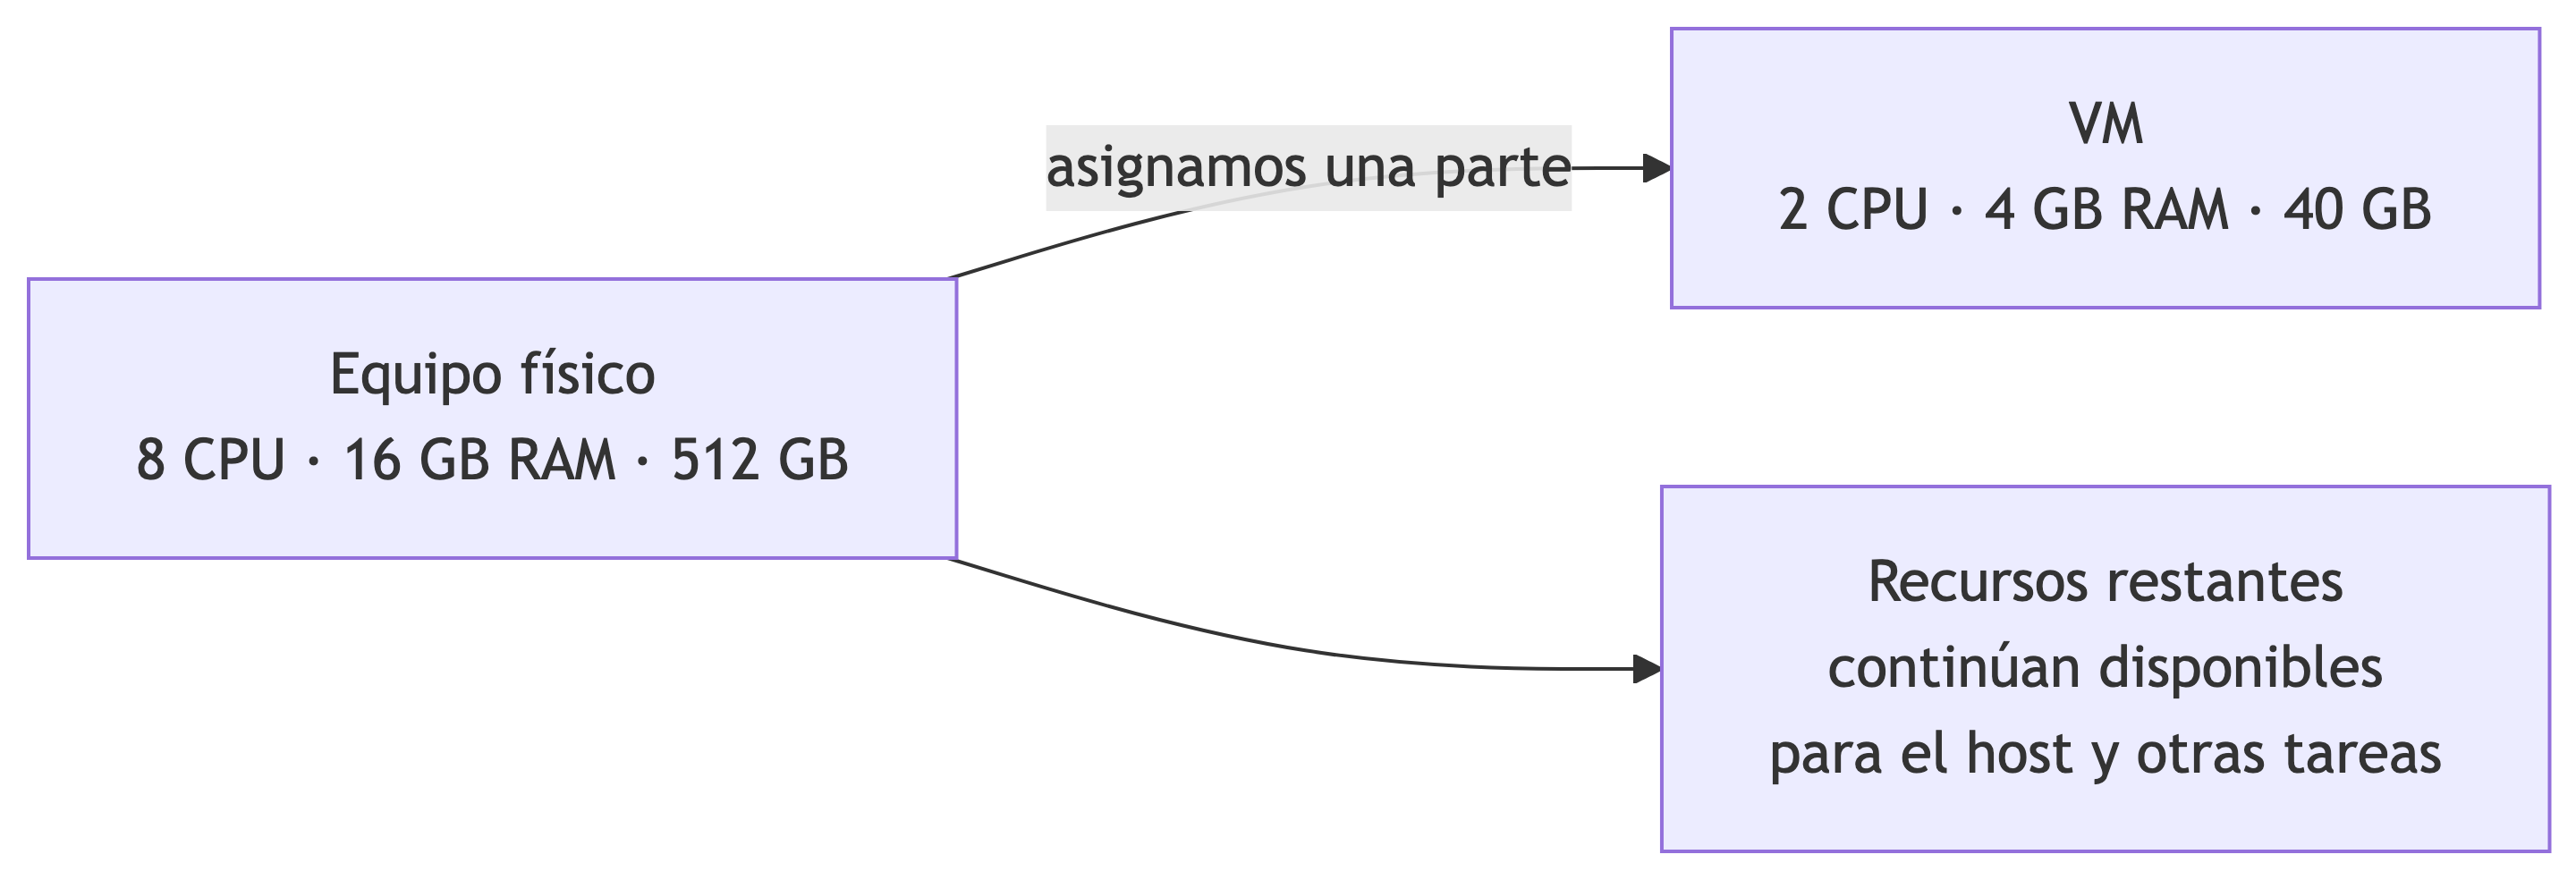
\includegraphics[width=7.3in,height=4.7in]{capitulos/12_virtualizacion_sistemas_operativos_files/figure-latex/mermaid-figure-4.png}

\begin{tcolorbox}[enhanced jigsaw, arc=.35mm, bottomrule=.15mm, bottomtitle=1mm, breakable, colback=white, colbacktitle=quarto-callout-warning-color!10!white, colframe=quarto-callout-warning-color-frame, coltitle=black, left=2mm, leftrule=.75mm, opacityback=0, opacitybacktitle=0.6, rightrule=.15mm, title=\textcolor{quarto-callout-warning-color}{\faExclamationTriangle}\hspace{0.5em}{No debemos entregar todo a la VM}, titlerule=0mm, toprule=.15mm, toptitle=1mm]

El Sistema Operativo anfitrión también necesita CPU y RAM. Asignar
demasiados recursos a una VM puede hacer lento al host y,
paradójicamente, empeorar toda la experiencia.

\end{tcolorbox}

\begin{center}\rule{0.5\linewidth}{0.5pt}\end{center}

\bookmarksetup{startatroot}

\chapter{4. Una VM no es simplemente otra
ventana}\label{una-vm-no-es-simplemente-otra-ventana}

Cuando abrimos una VM vemos una ventana, pero detrás existe una
computadora virtual completa.

El hipervisor puede presentar al guest:

\begin{itemize}
\tightlist
\item
  procesadores virtuales;
\item
  memoria RAM;
\item
  almacenamiento;
\item
  tarjeta de red;
\item
  controlador gráfico;
\item
  dispositivos USB;
\item
  firmware virtual;
\item
  otros dispositivos.
\end{itemize}

El guest utiliza esos dispositivos como si pertenecieran a una
computadora real.

\begin{center}\rule{0.5\linewidth}{0.5pt}\end{center}

\bookmarksetup{startatroot}

\chapter{5. ¿Para qué virtualizamos?}\label{para-quuxe9-virtualizamos}

La virtualización resulta especialmente útil para:

\begin{itemize}
\tightlist
\item
  aprender otros Sistemas Operativos;
\item
  practicar administración sin modificar el equipo principal;
\item
  probar software;
\item
  construir laboratorios;
\item
  simular servidores;
\item
  realizar pruebas de redes;
\item
  crear entornos aislados;
\item
  probar configuraciones antes de utilizarlas en producción;
\item
  ejecutar aplicaciones que requieren otro Sistema Operativo.
\end{itemize}

\begin{tcolorbox}[enhanced jigsaw, arc=.35mm, bottomrule=.15mm, bottomtitle=1mm, breakable, colback=white, colbacktitle=quarto-callout-tip-color!10!white, colframe=quarto-callout-tip-color-frame, coltitle=black, left=2mm, leftrule=.75mm, opacityback=0, opacitybacktitle=0.6, rightrule=.15mm, title=\textcolor{quarto-callout-tip-color}{\faLightbulb}\hspace{0.5em}{En nuestro curso}, titlerule=0mm, toprule=.15mm, toptitle=1mm]

Una VM funciona como un \textbf{laboratorio dentro de nuestra
computadora}. Podemos experimentar, equivocarnos, reinstalar y volver a
intentar sin tener que modificar directamente el Sistema Operativo
principal.

\end{tcolorbox}

\begin{center}\rule{0.5\linewidth}{0.5pt}\end{center}

\bookmarksetup{startatroot}

\chapter{6. ¿Qué ocurre si algo sale
mal?}\label{quuxe9-ocurre-si-algo-sale-mal}

Una de las ventajas de una VM es el aislamiento.

Un error dentro del guest normalmente no significa que tengamos que
reinstalar el host.

Además, muchas plataformas permiten crear \textbf{snapshots}.

\section{Snapshot: el punto de
guardado}\label{snapshot-el-punto-de-guardado}

Podemos imaginar un snapshot como el \textbf{punto de guardado de un
videojuego}.

\begin{Shaded}
\begin{Highlighting}[]
\NormalTok{VM recién instalada}
\NormalTok{       ↓}
\NormalTok{[Snapshot A]}
\NormalTok{       ↓}
\NormalTok{Instalamos programas}
\NormalTok{       ↓}
\NormalTok{[Snapshot B]}
\NormalTok{       ↓}
\NormalTok{Hacemos una prueba peligrosa}
\NormalTok{       ↓}
\NormalTok{Algo sale mal}
\NormalTok{       ↓}
\NormalTok{Regresamos al Snapshot B}
\end{Highlighting}
\end{Shaded}

\begin{tcolorbox}[enhanced jigsaw, arc=.35mm, bottomrule=.15mm, bottomtitle=1mm, breakable, colback=white, colbacktitle=quarto-callout-warning-color!10!white, colframe=quarto-callout-warning-color-frame, coltitle=black, left=2mm, leftrule=.75mm, opacityback=0, opacitybacktitle=0.6, rightrule=.15mm, title=\textcolor{quarto-callout-warning-color}{\faExclamationTriangle}\hspace{0.5em}{Snapshot no significa backup completo}, titlerule=0mm, toprule=.15mm, toptitle=1mm]

Un snapshot es muy útil para regresar rápidamente a un estado anterior
de una VM, pero no debe confundirse con una estrategia completa de
copias de seguridad.

\end{tcolorbox}

\begin{center}\rule{0.5\linewidth}{0.5pt}\end{center}

\bookmarksetup{startatroot}

\chapter{7. ISO, disco virtual y Sistema
Operativo}\label{iso-disco-virtual-y-sistema-operativo}

Estos conceptos suelen confundirse al comenzar.

\section{Imagen ISO}\label{imagen-iso}

Una \textbf{ISO} contiene una imagen de un medio de instalación.

Podemos imaginarla como el equivalente digital del DVD o USB desde el
cual instalaríamos un Sistema Operativo.

\section{Disco virtual}\label{disco-virtual}

Es un archivo que el guest interpreta como si fuera un disco duro o SSD.

En VirtualBox es común encontrar formatos como \textbf{VDI}; otras
plataformas utilizan formatos diferentes.

\section{La relación}\label{la-relaciuxf3n}

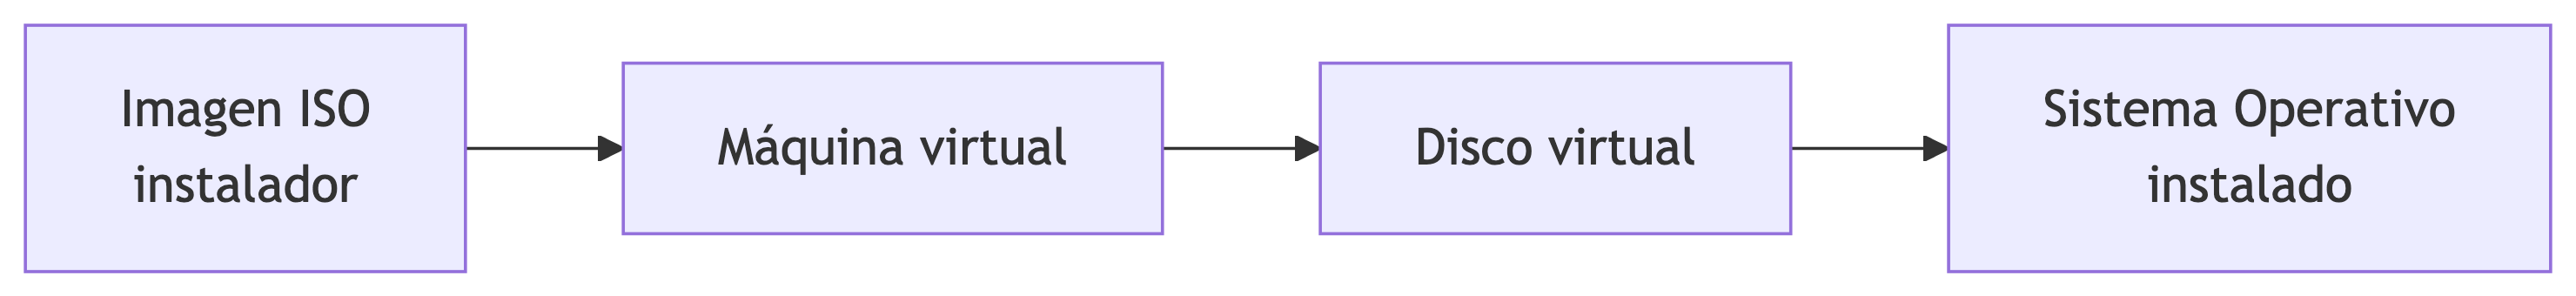
\includegraphics[width=7in,height=4.3in]{capitulos/12_virtualizacion_sistemas_operativos_files/figure-latex/mermaid-figure-3.png}

\begin{tcolorbox}[enhanced jigsaw, arc=.35mm, bottomrule=.15mm, bottomtitle=1mm, breakable, colback=white, colbacktitle=quarto-callout-note-color!10!white, colframe=quarto-callout-note-color-frame, coltitle=black, left=2mm, leftrule=.75mm, opacityback=0, opacitybacktitle=0.6, rightrule=.15mm, title=\textcolor{quarto-callout-note-color}{\faInfo}\hspace{0.5em}{Una comparación sencilla}, titlerule=0mm, toprule=.15mm, toptitle=1mm]

\textbf{ISO = instalador.}\\
\textbf{Disco virtual = lugar donde quedará instalado el Sistema
Operativo.}

\end{tcolorbox}

\begin{center}\rule{0.5\linewidth}{0.5pt}\end{center}

\bookmarksetup{startatroot}

\chapter{8. Antes de descargar: x86-64 y
ARM64}\label{antes-de-descargar-x86-64-y-arm64}

\begin{figure}[H]

{\centering 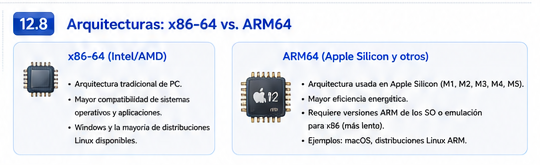
\includegraphics[width=0.88\linewidth,height=\textheight,keepaspectratio]{capitulos/img/capitulo12/arquitecturas_x86_arm64.png}

}

\caption{Comparación didáctica entre equipos x86-64 y ARM64 al elegir
una máquina virtual.}

\end{figure}%

Este es uno de los cambios más importantes respecto de muchos materiales
antiguos de virtualización.

Actualmente podemos encontrar computadoras con diferentes arquitecturas.

\section{x86-64}\label{x86-64}

Es común en equipos con procesadores:

\begin{itemize}
\tightlist
\item
  Intel;
\item
  AMD.
\end{itemize}

\section{ARM64}\label{arm64}

Actualmente aparece, entre otros, en:

\begin{itemize}
\tightlist
\item
  Mac con Apple Silicon;
\item
  algunos equipos Windows con procesadores ARM.
\end{itemize}

\begin{tcolorbox}[enhanced jigsaw, arc=.35mm, bottomrule=.15mm, bottomtitle=1mm, breakable, colback=white, colbacktitle=quarto-callout-important-color!10!white, colframe=quarto-callout-important-color-frame, coltitle=black, left=2mm, leftrule=.75mm, opacityback=0, opacitybacktitle=0.6, rightrule=.15mm, title=\textcolor{quarto-callout-important-color}{\faExclamation}\hspace{0.5em}{La arquitectura importa}, titlerule=0mm, toprule=.15mm, toptitle=1mm]

No debemos asumir que cualquier ISO funcionará de la misma manera en
cualquier computadora.

Un Mac Apple Silicon utiliza arquitectura \textbf{ARM64}. Por eso
conviene utilizar Sistemas Operativos invitados y herramientas
compatibles con ARM64 cuando queremos virtualización eficiente.

\end{tcolorbox}

\begin{center}\rule{0.5\linewidth}{0.5pt}\end{center}

\bookmarksetup{startatroot}

\chapter{9. Virtualización y emulación no son lo
mismo}\label{virtualizaciuxf3n-y-emulaciuxf3n-no-son-lo-mismo}

\begin{figure}[H]

{\centering 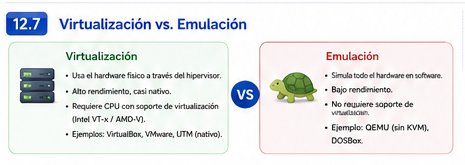
\includegraphics[width=0.88\linewidth,height=\textheight,keepaspectratio]{capitulos/img/capitulo12/virtualizacion_vs_emulacion.png}

}

\caption{Virtualización y emulación: dos caminos distintos para ejecutar
sistemas invitados.}

\end{figure}%

\section{Virtualización}\label{virtualizaciuxf3n}

Cuando host y guest utilizan arquitecturas compatibles, el software
puede aprovechar directamente las capacidades de virtualización del
procesador.

Resultado habitual:

\begin{quote}
\textbf{mejor rendimiento.}
\end{quote}

\section{Emulación}\label{emulaciuxf3n}

La emulación reproduce mediante software el comportamiento de otra
arquitectura.

Ejemplo conceptual:

\begin{Shaded}
\begin{Highlighting}[]
\NormalTok{Host ARM64}
\NormalTok{    ↓}
\NormalTok{Emular x86{-}64}
\NormalTok{    ↓}
\NormalTok{Guest x86{-}64}
\end{Highlighting}
\end{Shaded}

Esto permite escenarios que la virtualización directa no permite, pero
normalmente tiene un costo de rendimiento.

{\def\LTcaptype{none} % do not increment counter
\begin{longtable}[]{@{}
  >{\raggedright\arraybackslash}p{(\linewidth - 4\tabcolsep) * \real{0.3333}}
  >{\raggedright\arraybackslash}p{(\linewidth - 4\tabcolsep) * \real{0.3333}}
  >{\raggedright\arraybackslash}p{(\linewidth - 4\tabcolsep) * \real{0.3333}}@{}}
\toprule\noalign{}
\begin{minipage}[b]{\linewidth}\raggedright
Característica
\end{minipage} & \begin{minipage}[b]{\linewidth}\raggedright
Virtualización
\end{minipage} & \begin{minipage}[b]{\linewidth}\raggedright
Emulación
\end{minipage} \\
\midrule\noalign{}
\endhead
\bottomrule\noalign{}
\endlastfoot
Arquitectura & Normalmente compatible & Puede ser diferente \\
Rendimiento & Generalmente mayor & Generalmente menor \\
Uso típico & VM cotidiana & Compatibilidad o sistemas de otra
arquitectura \\
\end{longtable}
}

\begin{center}\rule{0.5\linewidth}{0.5pt}\end{center}

\bookmarksetup{startatroot}

\chapter{10. ¿Qué programa podemos utilizar en
2026?}\label{quuxe9-programa-podemos-utilizar-en-2026}

No existe una única respuesta correcta. La herramienta depende del
Sistema Operativo anfitrión, arquitectura y objetivo.

{\def\LTcaptype{none} % do not increment counter
\begin{longtable}[]{@{}
  >{\raggedright\arraybackslash}p{(\linewidth - 8\tabcolsep) * \real{0.1429}}
  >{\centering\arraybackslash}p{(\linewidth - 8\tabcolsep) * \real{0.2381}}
  >{\centering\arraybackslash}p{(\linewidth - 8\tabcolsep) * \real{0.2381}}
  >{\centering\arraybackslash}p{(\linewidth - 8\tabcolsep) * \real{0.2381}}
  >{\raggedright\arraybackslash}p{(\linewidth - 8\tabcolsep) * \real{0.1429}}@{}}
\toprule\noalign{}
\begin{minipage}[b]{\linewidth}\raggedright
Herramienta
\end{minipage} & \begin{minipage}[b]{\linewidth}\centering
Windows
\end{minipage} & \begin{minipage}[b]{\linewidth}\centering
Mac Intel
\end{minipage} & \begin{minipage}[b]{\linewidth}\centering
Mac Apple Silicon
\end{minipage} & \begin{minipage}[b]{\linewidth}\raggedright
Comentario
\end{minipage} \\
\midrule\noalign{}
\endhead
\bottomrule\noalign{}
\endlastfoot
\textbf{Oracle VirtualBox} & ✓ & ✓ & ✓ & Multiplataforma; verificar
compatibilidad host/guest \\
\textbf{VMware Workstation} & ✓ & --- & --- & Alternativa sólida para
Windows/Linux \\
\textbf{VMware Fusion} & --- & ✓ & ✓ & Diseñado para macOS \\
\textbf{UTM} & --- & ✓ & ✓ & Muy útil en Mac; permite virtualización y
escenarios de emulación \\
\end{longtable}
}

\begin{tcolorbox}[enhanced jigsaw, arc=.35mm, bottomrule=.15mm, bottomtitle=1mm, breakable, colback=white, colbacktitle=quarto-callout-tip-color!10!white, colframe=quarto-callout-tip-color-frame, coltitle=black, left=2mm, leftrule=.75mm, opacityback=0, opacitybacktitle=0.6, rightrule=.15mm, title=\textcolor{quarto-callout-tip-color}{\faLightbulb}\hspace{0.5em}{¿Cuál utilizaremos?}, titlerule=0mm, toprule=.15mm, toptitle=1mm]

Para comprender los conceptos, cualquiera de estas herramientas puede
servir. En clase podemos trabajar con \textbf{VirtualBox} como
referencia y mostrar alternativas para estudiantes cuyo hardware o
Sistema Operativo requiera otra opción.

\end{tcolorbox}

\begin{center}\rule{0.5\linewidth}{0.5pt}\end{center}

\bookmarksetup{startatroot}

\chapter{11. Descargas oficiales}\label{descargas-oficiales}

Los enlaces siguientes deben utilizarse como punto de partida. Evitemos
descargar hipervisores o imágenes ISO desde sitios desconocidos.

\section{Hipervisores}\label{hipervisores}

\begin{itemize}
\tightlist
\item
  \href{https://www.virtualbox.org/wiki/Downloads}{Oracle VirtualBox}
\item
  \href{https://knowledge.broadcom.com/external/article/368734/download-desktop-hypervisor-workstation.html}{VMware
  Workstation / VMware Fusion --- instrucciones oficiales de Broadcom}
\item
  \href{https://mac.getutm.app/}{UTM para macOS}
\end{itemize}

\section{Sistemas Operativos}\label{sistemas-operativos}

\begin{itemize}
\tightlist
\item
  \href{https://www.microsoft.com/software-download/windows11}{Windows
  11}
\item
  \href{https://ubuntu.com/download/desktop}{Ubuntu Desktop}
\item
  \href{https://www.debian.org/distrib/}{Debian}
\item
  \href{https://fedoraproject.org/}{Fedora}
\item
  \href{https://linuxmint.com/download.php}{Linux Mint}
\end{itemize}

\begin{tcolorbox}[enhanced jigsaw, arc=.35mm, bottomrule=.15mm, bottomtitle=1mm, breakable, colback=white, colbacktitle=quarto-callout-note-color!10!white, colframe=quarto-callout-note-color-frame, coltitle=black, left=2mm, leftrule=.75mm, opacityback=0, opacitybacktitle=0.6, rightrule=.15mm, title=\textcolor{quarto-callout-note-color}{\faInfo}\hspace{0.5em}{VMware en la actualidad}, titlerule=0mm, toprule=.15mm, toptitle=1mm]

VMware Workstation Pro y VMware Fusion Pro cuentan con versiones
gratuitas para usuarios personales, educativos y comerciales. Broadcom
solicita una cuenta básica para acceder a las descargas.

\end{tcolorbox}

\begin{center}\rule{0.5\linewidth}{0.5pt}\end{center}

\bookmarksetup{startatroot}

\chapter{12. ¿Qué debería elegir un
estudiante?}\label{quuxe9-deberuxeda-elegir-un-estudiante}

\section{Caso A: PC Windows Intel/AMD}\label{caso-a-pc-windows-intelamd}

Una opción sencilla:

\begin{Shaded}
\begin{Highlighting}[]
\NormalTok{Host: Windows 10/11}
\NormalTok{Arquitectura: x86{-}64}
\NormalTok{Herramienta: VirtualBox o VMware Workstation}
\NormalTok{Guest: Ubuntu x86{-}64}
\end{Highlighting}
\end{Shaded}

\section{Caso B: Mac Intel}\label{caso-b-mac-intel}

\begin{Shaded}
\begin{Highlighting}[]
\NormalTok{Host: macOS}
\NormalTok{Arquitectura: x86{-}64}
\NormalTok{Herramienta: VirtualBox o VMware Fusion}
\NormalTok{Guest: Linux x86{-}64}
\end{Highlighting}
\end{Shaded}

\section{Caso C: Mac Apple Silicon}\label{caso-c-mac-apple-silicon}

\begin{Shaded}
\begin{Highlighting}[]
\NormalTok{Host: macOS}
\NormalTok{Arquitectura: ARM64}
\NormalTok{Herramienta: VirtualBox, VMware Fusion o UTM}
\NormalTok{Guest recomendado: versión ARM64 compatible}
\end{Highlighting}
\end{Shaded}

\begin{tcolorbox}[enhanced jigsaw, arc=.35mm, bottomrule=.15mm, bottomtitle=1mm, breakable, colback=white, colbacktitle=quarto-callout-warning-color!10!white, colframe=quarto-callout-warning-color-frame, coltitle=black, left=2mm, leftrule=.75mm, opacityback=0, opacitybacktitle=0.6, rightrule=.15mm, title=\textcolor{quarto-callout-warning-color}{\faExclamationTriangle}\hspace{0.5em}{Especialmente importante en Apple Silicon}, titlerule=0mm, toprule=.15mm, toptitle=1mm]

No basta con leer ``Ubuntu'', ``Windows'' o ``Linux''. Debemos verificar
también \textbf{para qué arquitectura fue construida la imagen}.

\end{tcolorbox}

\begin{center}\rule{0.5\linewidth}{0.5pt}\end{center}

\bookmarksetup{startatroot}

\chapter{13. ¿Cuánta RAM, CPU y disco
asignamos?}\label{cuuxe1nta-ram-cpu-y-disco-asignamos}

No existe una cantidad universal.

Debemos considerar:

\begin{enumerate}
\def\labelenumi{\arabic{enumi}.}
\tightlist
\item
  recursos físicos del host;
\item
  requisitos del guest;
\item
  aplicaciones que ejecutaremos;
\item
  cuántas VMs estarán encendidas simultáneamente.
\end{enumerate}

\section{Ejemplo didáctico}\label{ejemplo-diduxe1ctico}

Equipo físico:

\begin{Shaded}
\begin{Highlighting}[]
\NormalTok{16 GB RAM}
\NormalTok{8 núcleos}
\NormalTok{512 GB almacenamiento}
\end{Highlighting}
\end{Shaded}

VM Linux para prácticas:

\begin{Shaded}
\begin{Highlighting}[]
\NormalTok{4 GB RAM}
\NormalTok{2 CPU virtuales}
\NormalTok{40 GB disco virtual}
\end{Highlighting}
\end{Shaded}

Esto \textbf{no es una regla obligatoria}. Es solamente un punto de
partida razonable para un laboratorio sencillo.

\begin{center}\rule{0.5\linewidth}{0.5pt}\end{center}

\bookmarksetup{startatroot}

\chapter{14. Flujo para crear una máquina
virtual}\label{flujo-para-crear-una-muxe1quina-virtual}

Antes de presionar botones, comprendamos el proceso.

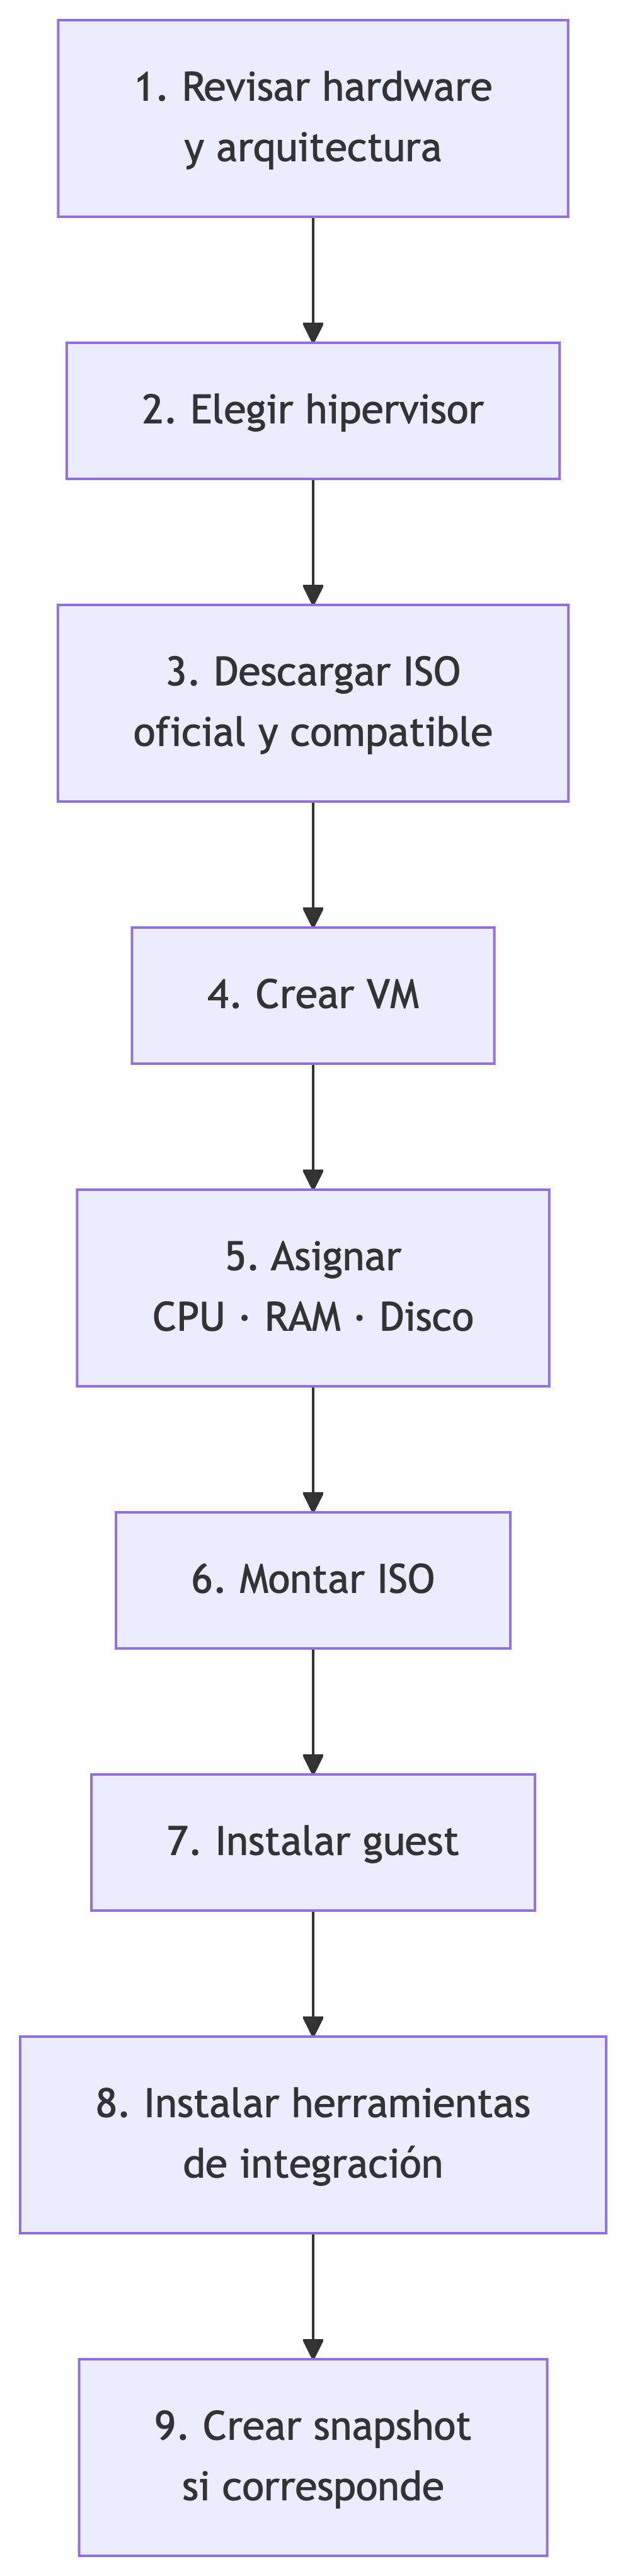
\includegraphics[width=6.7in,height=7in]{capitulos/12_virtualizacion_sistemas_operativos_files/figure-latex/mermaid-figure-2.png}

\begin{tcolorbox}[enhanced jigsaw, arc=.35mm, bottomrule=.15mm, bottomtitle=1mm, breakable, colback=white, colbacktitle=quarto-callout-important-color!10!white, colframe=quarto-callout-important-color-frame, coltitle=black, left=2mm, leftrule=.75mm, opacityback=0, opacitybacktitle=0.6, rightrule=.15mm, title=\textcolor{quarto-callout-important-color}{\faExclamation}\hspace{0.5em}{Primero diseñamos; después instalamos}, titlerule=0mm, toprule=.15mm, toptitle=1mm]

La creación de una VM no debería comenzar haciendo clic al azar. Antes
debemos saber:

\textbf{qué quiero instalar + qué arquitectura tengo + qué recursos
puedo asignar + qué herramienta es compatible.}

\end{tcolorbox}

\begin{center}\rule{0.5\linewidth}{0.5pt}\end{center}

\bookmarksetup{startatroot}

\chapter{15. Actividad guiada: diseñemos una VM sin instalar
nada}\label{actividad-guiada-diseuxf1emos-una-vm-sin-instalar-nada}

Tenemos una computadora:

\begin{Shaded}
\begin{Highlighting}[]
\NormalTok{Windows 11}
\NormalTok{Intel Core i5}
\NormalTok{16 GB RAM}
\NormalTok{512 GB SSD}
\NormalTok{120 GB disponibles}
\end{Highlighting}
\end{Shaded}

Queremos practicar comandos Linux utilizando Ubuntu.

Responde:

\begin{enumerate}
\def\labelenumi{\arabic{enumi}.}
\tightlist
\item
  ¿Cuál será el host?
\item
  ¿Cuál será el guest?
\item
  ¿Qué arquitectura debemos verificar?
\item
  ¿Qué herramientas podríamos utilizar?
\item
  ¿Cuánta RAM asignarías?
\item
  ¿Cuántas CPU virtuales?
\item
  ¿Cuánto disco virtual?
\item
  ¿Qué archivo debemos descargar para iniciar la instalación?
\item
  ¿Crearías un snapshot después de instalar Ubuntu? ¿Por qué?
\end{enumerate}

\begin{tcolorbox}[enhanced jigsaw, arc=.35mm, bottomrule=.15mm, bottomtitle=1mm, breakable, colback=white, colbacktitle=quarto-callout-tip-color!10!white, colframe=quarto-callout-tip-color-frame, coltitle=black, left=2mm, leftrule=.75mm, opacityback=0, opacitybacktitle=0.6, rightrule=.15mm, title=\textcolor{quarto-callout-tip-color}{\faLightbulb}\hspace{0.5em}{✅ Ver una posible solución}, titlerule=0mm, toprule=.15mm, toptitle=1mm]

\begin{enumerate}
\def\labelenumi{\arabic{enumi}.}
\tightlist
\item
  \textbf{Host:} Windows 11.
\item
  \textbf{Guest:} Ubuntu.
\item
  Debemos comprobar la arquitectura del procesador y descargar una ISO
  compatible; en este caso normalmente x86-64.
\item
  VirtualBox o VMware Workstation son opciones posibles.
\item
  Para una práctica sencilla podrían asignarse aproximadamente \textbf{4
  GB de RAM}, siempre que el host conserve recursos suficientes.
\item
  \textbf{2 CPU virtuales} pueden ser un punto de partida.
\item
  Un disco virtual de aproximadamente \textbf{30--40 GB} puede ser
  suficiente para un laboratorio básico, sujeto a los requisitos de la
  versión instalada.
\item
  Una \textbf{imagen ISO oficial de Ubuntu}.
\item
  Sí. Un snapshot posterior a una instalación limpia permite regresar
  rápidamente a ese estado antes de experimentar.
\end{enumerate}

La configuración no es única. Lo importante es \textbf{justificarla}.

\end{tcolorbox}

\begin{center}\rule{0.5\linewidth}{0.5pt}\end{center}

\bookmarksetup{startatroot}

\chapter{16. Mini reto: tú eres el
administrador}\label{mini-reto-tuxfa-eres-el-administrador}

Analiza los tres equipos.

\subsection{Equipo A}\label{equipo-a}

\begin{Shaded}
\begin{Highlighting}[]
\NormalTok{Windows 11}
\NormalTok{AMD Ryzen}
\NormalTok{8 GB RAM}
\NormalTok{256 GB SSD}
\end{Highlighting}
\end{Shaded}

\subsection{Equipo B}\label{equipo-b}

\begin{Shaded}
\begin{Highlighting}[]
\NormalTok{Windows 11}
\NormalTok{Intel}
\NormalTok{32 GB RAM}
\NormalTok{1 TB SSD}
\end{Highlighting}
\end{Shaded}

\subsection{Equipo C}\label{equipo-c}

\begin{Shaded}
\begin{Highlighting}[]
\NormalTok{MacBook Apple Silicon}
\NormalTok{16 GB RAM}
\NormalTok{512 GB SSD}
\end{Highlighting}
\end{Shaded}

Para cada equipo decide:

\begin{enumerate}
\def\labelenumi{\arabic{enumi}.}
\tightlist
\item
  herramienta de virtualización;
\item
  guest que instalarías;
\item
  arquitectura del guest;
\item
  RAM;
\item
  CPU virtual;
\item
  disco;
\item
  si utilizarías snapshot.
\end{enumerate}

Luego responde:

\begin{quote}
\textbf{¿En cuál equipo tendrías mayor libertad para ejecutar varias VMs
simultáneamente y por qué?}
\end{quote}

Tiempo sugerido: \textbf{10 minutos}.

\begin{center}\rule{0.5\linewidth}{0.5pt}\end{center}

\bookmarksetup{startatroot}

\chapter{17. Errores comunes al
comenzar}\label{errores-comunes-al-comenzar}

\section{``Le asignaré toda la RAM a la
VM''}\label{le-asignaruxe9-toda-la-ram-a-la-vm}

Incorrecto. El host también necesita memoria.

\section{``Descargué cualquier ISO de
Internet''}\label{descarguuxe9-cualquier-iso-de-internet}

Debemos utilizar fuentes oficiales y comprobar arquitectura.

\section{``Si tengo Apple Silicon puedo ejecutar cualquier x86 como si
fuera
nativo''}\label{si-tengo-apple-silicon-puedo-ejecutar-cualquier-x86-como-si-fuera-nativo}

No necesariamente. Debemos distinguir virtualización de emulación.

\section{``Snapshot significa que ya tengo
backup''}\label{snapshot-significa-que-ya-tengo-backup}

No.~Son conceptos relacionados con recuperación, pero no equivalentes.

\section{``VirtualBox es la única
opción''}\label{virtualbox-es-la-uxfanica-opciuxf3n}

No.~Es una herramienta muy conocida, pero existen alternativas.

\begin{center}\rule{0.5\linewidth}{0.5pt}\end{center}

\bookmarksetup{startatroot}

\chapter{18. Autoevaluación}\label{autoevaluaciuxf3n-7}

\begin{enumerate}
\def\labelenumi{\arabic{enumi}.}
\tightlist
\item
  ¿Qué es una máquina virtual?
\item
  ¿Qué función cumple un hipervisor?
\item
  ¿Qué diferencia existe entre host y guest?
\item
  ¿De dónde obtiene RAM una VM?
\item
  ¿Qué es una imagen ISO?
\item
  ¿Qué diferencia existe entre ISO y disco virtual?
\item
  ¿Qué es un snapshot?
\item
  ¿Por qué un snapshot no sustituye necesariamente un backup?
\item
  ¿Qué significa x86-64?
\item
  ¿Qué significa ARM64?
\item
  ¿Por qué la arquitectura es especialmente importante en Apple Silicon?
\item
  ¿Cuál es la diferencia conceptual entre virtualización y emulación?
\item
  Menciona dos alternativas a VirtualBox.
\item
  ¿Qué criterios utilizarías para decidir cuánta RAM asignar a una VM?
\item
  ¿Por qué no conviene descargar imágenes ISO desde sitios desconocidos?
\end{enumerate}

\begin{center}\rule{0.5\linewidth}{0.5pt}\end{center}

\bookmarksetup{startatroot}

\chapter{19. Para recordar}\label{para-recordar-3}

\begin{quote}
\textbf{Virtualizar no significa crear recursos nuevos: significa
administrar y presentar recursos físicos de forma virtual.}
\end{quote}

Antes de crear una VM debemos responder:

\begin{Shaded}
\begin{Highlighting}[]
\NormalTok{¿Qué quiero instalar?}
\NormalTok{        ↓}
\NormalTok{¿Qué arquitectura tiene mi host?}
\NormalTok{        ↓}
\NormalTok{¿Qué arquitectura necesita el guest?}
\NormalTok{        ↓}
\NormalTok{¿Qué hipervisor es compatible?}
\NormalTok{        ↓}
\NormalTok{¿Cuántos recursos puedo asignar?}
\NormalTok{        ↓}
\NormalTok{¿Qué ISO debo descargar?}
\end{Highlighting}
\end{Shaded}

\begin{center}\rule{0.5\linewidth}{0.5pt}\end{center}

\bookmarksetup{startatroot}

\chapter{20. Síntesis visual del
capítulo}\label{suxedntesis-visual-del-capuxedtulo}

\begin{figure}[H]

{\centering 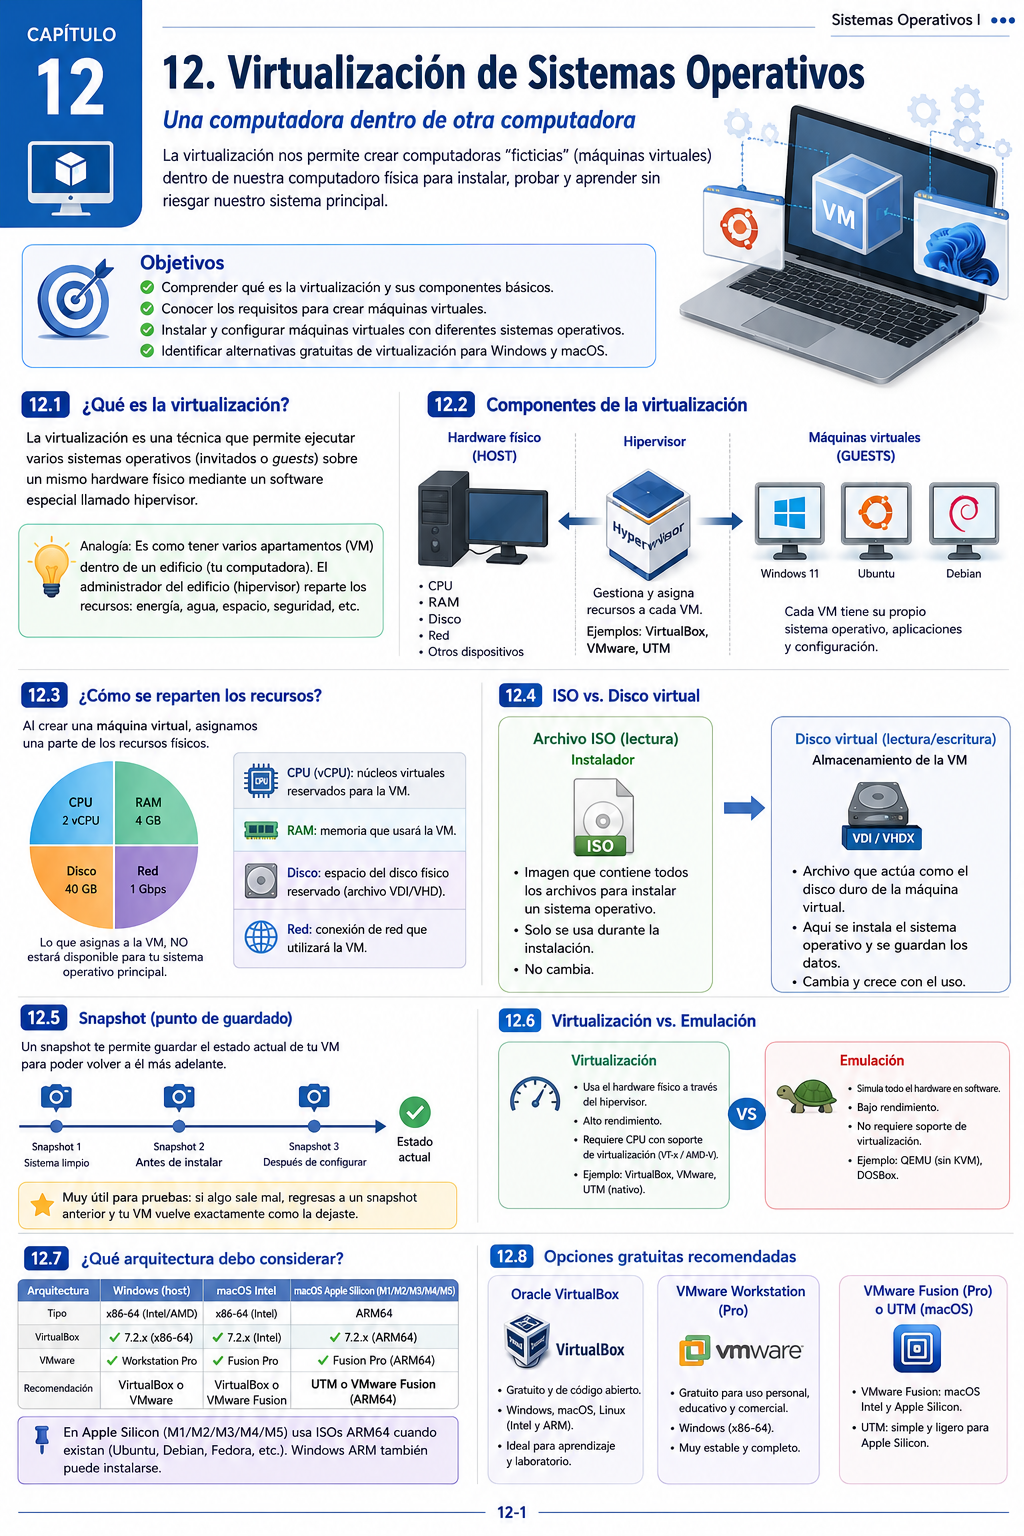
\includegraphics[width=0.96\linewidth,height=\textheight,keepaspectratio]{capitulos/img/capitulo12/sintesis_virtualizacion_so.png}

}

\caption{Síntesis visual del capítulo 12: virtualización de Sistemas
Operativos.}

\end{figure}%

La síntesis visual debe permitir reconstruir el tema completo mediante
cinco ideas:

\begin{Shaded}
\begin{Highlighting}[]
\NormalTok{COMPUTADORA FÍSICA}
\NormalTok{        ↓}
\NormalTok{HOST}
\NormalTok{        ↓}
\NormalTok{HIPERVISOR}
\NormalTok{        ↓}
\NormalTok{MÁQUINA VIRTUAL}
\NormalTok{        ↓}
\NormalTok{GUEST}
\end{Highlighting}
\end{Shaded}

y relacionarlas con:

\begin{Shaded}
\begin{Highlighting}[]
\NormalTok{CPU · RAM · DISCO · RED}
\NormalTok{ISO · DISCO VIRTUAL · SNAPSHOT}
\NormalTok{x86{-}64 · ARM64}
\NormalTok{VIRTUALIZACIÓN · EMULACIÓN}
\end{Highlighting}
\end{Shaded}

\begin{tcolorbox}[enhanced jigsaw, arc=.35mm, bottomrule=.15mm, bottomtitle=1mm, breakable, colback=white, colbacktitle=quarto-callout-note-color!10!white, colframe=quarto-callout-note-color-frame, coltitle=black, left=2mm, leftrule=.75mm, opacityback=0, opacitybacktitle=0.6, rightrule=.15mm, title=\textcolor{quarto-callout-note-color}{\faInfo}\hspace{0.5em}{Síntesis en una frase}, titlerule=0mm, toprule=.15mm, toptitle=1mm]

\textbf{Una máquina virtual es una computadora definida por software que
utiliza recursos administrados del hardware físico para ejecutar su
propio Sistema Operativo.}

\end{tcolorbox}

\begin{center}\rule{0.5\linewidth}{0.5pt}\end{center}

\bookmarksetup{startatroot}

\chapter{Conexión con la siguiente
clase}\label{conexiuxf3n-con-la-siguiente-clase-1}

Ahora comprendemos qué es una máquina virtual, qué recursos utiliza y
cómo seleccionar una plataforma.

El siguiente paso natural será \textbf{crear una VM real}, instalar un
Sistema Operativo invitado y observar cómo se comportan CPU, memoria,
almacenamiento y red durante la ejecución.

\begin{center}\rule{0.5\linewidth}{0.5pt}\end{center}

\bookmarksetup{startatroot}

\chapter{Referencias y
actualización}\label{referencias-y-actualizaciuxf3n-1}

Material base de clase:

\begin{itemize}
\tightlist
\item
  Presentación \textbf{Virtualización de Sistemas Operativos}, edición
  2025.
\end{itemize}

Documentación oficial recomendada:

\begin{itemize}
\tightlist
\item
  Oracle VirtualBox --- documentación y descargas oficiales.
\item
  Broadcom --- VMware Workstation Pro y VMware Fusion Pro.
\item
  UTM --- documentación oficial.
\item
  Microsoft --- descargas oficiales de Windows.
\item
  Ubuntu, Debian, Fedora y Linux Mint --- sitios oficiales de
  distribución.
\end{itemize}

\begin{tcolorbox}[enhanced jigsaw, arc=.35mm, bottomrule=.15mm, bottomtitle=1mm, breakable, colback=white, colbacktitle=quarto-callout-tip-color!10!white, colframe=quarto-callout-tip-color-frame, coltitle=black, left=2mm, leftrule=.75mm, opacityback=0, opacitybacktitle=0.6, rightrule=.15mm, title=\textcolor{quarto-callout-tip-color}{\faLightbulb}\hspace{0.5em}{Criterio editorial}, titlerule=0mm, toprule=.15mm, toptitle=1mm]

Las versiones de hipervisores y Sistemas Operativos cambian con
frecuencia. Por ello, este capítulo prioriza \textbf{conceptos y enlaces
oficiales} sobre números de versión que pueden quedar obsoletos.

\end{tcolorbox}

\bookmarksetup{startatroot}

\chapter{Capítulo 13. Manejo de memoria: particiones y
paginación}\label{capuxedtulo-13.-manejo-de-memoria-particiones-y-paginaciuxf3n}

\bookmarksetup{startatroot}

\chapter{Capítulo 13. Manejo de memoria: particiones y
paginación}\label{capuxedtulo-13.-manejo-de-memoria-particiones-y-paginaciuxf3n-1}

\section{¿Cómo caben tantos programas en la
memoria?}\label{cuxf3mo-caben-tantos-programas-en-la-memoria}

En una computadora podemos tener abierto el navegador, un editor de
código, música, una videollamada y otros programas al mismo tiempo.

Todos necesitan \textbf{memoria RAM}.

Pero la RAM es limitada.

Entonces aparece una pregunta fundamental:

\begin{quote}
\textbf{¿Cómo decide el Sistema Operativo qué parte de la memoria
utiliza cada proceso?}
\end{quote}

La respuesta nos lleva a uno de los trabajos más importantes del Sistema
Operativo: la \textbf{gestión de memoria}.

\begin{tcolorbox}[enhanced jigsaw, arc=.35mm, bottomrule=.15mm, bottomtitle=1mm, breakable, colback=white, colbacktitle=quarto-callout-tip-color!10!white, colframe=quarto-callout-tip-color-frame, coltitle=black, left=2mm, leftrule=.75mm, opacityback=0, opacitybacktitle=0.6, rightrule=.15mm, title=\textcolor{quarto-callout-tip-color}{\faLightbulb}\hspace{0.5em}{Idea central}, titlerule=0mm, toprule=.15mm, toptitle=1mm]

El Sistema Operativo debe \textbf{asignar, proteger, controlar y liberar
memoria} para que varios procesos puedan ejecutarse sin interferirse
entre sí.

\end{tcolorbox}

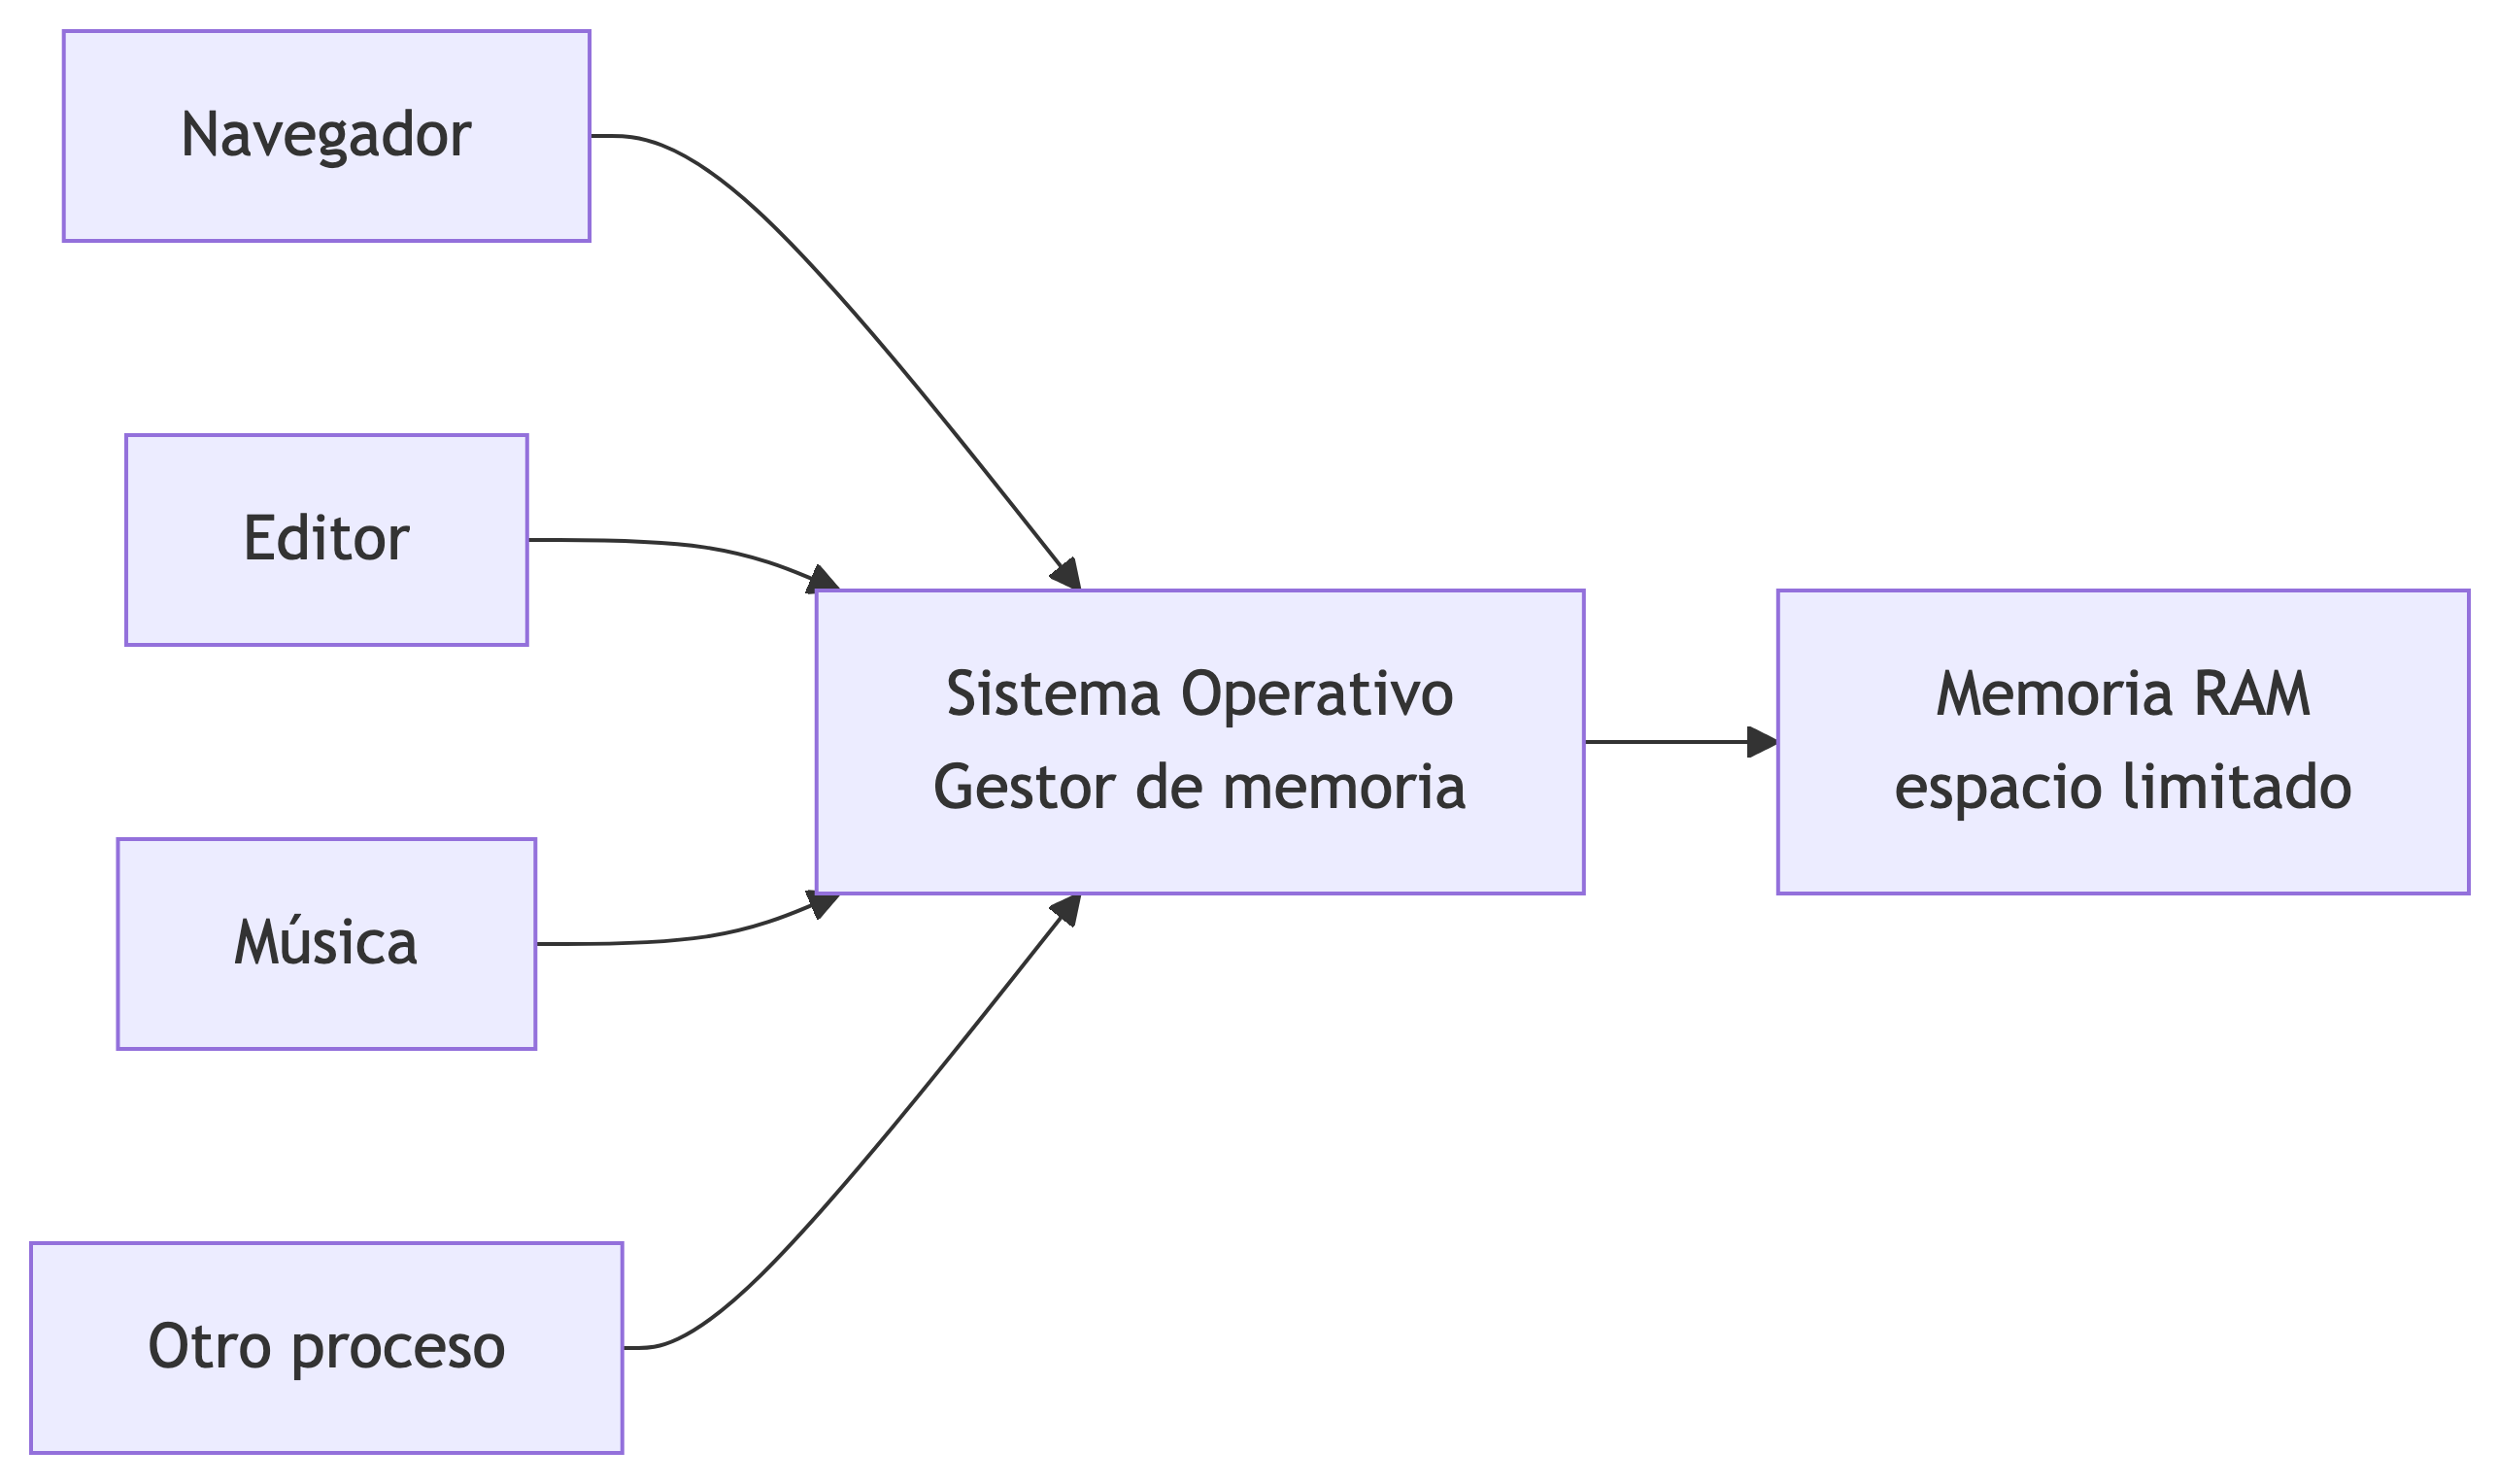
\includegraphics[width=7.3in,height=4.8in]{capitulos/13_manejo_memoria_paginacion_particiones_files/figure-latex/mermaid-figure-1.png}

\begin{center}\rule{0.5\linewidth}{0.5pt}\end{center}

\bookmarksetup{startatroot}

\chapter{Objetivos de aprendizaje}\label{objetivos-de-aprendizaje-9}

Al finalizar este capítulo, el estudiante será capaz de:

\begin{itemize}
\tightlist
\item
  Explicar por qué la gestión de memoria es una función crítica del
  Sistema Operativo.
\item
  Diferenciar una \textbf{dirección lógica} de una \textbf{dirección
  física}.
\item
  Comprender el funcionamiento de las \textbf{particiones fijas y
  dinámicas}.
\item
  Diferenciar \textbf{fragmentación interna} y \textbf{fragmentación
  externa}.
\item
  Aplicar conceptualmente los métodos \textbf{First Fit, Best Fit y
  Worst Fit}.
\item
  Explicar los conceptos de \textbf{página}, \textbf{marco} y
  \textbf{tabla de páginas}.
\item
  Comprender cómo se traduce una dirección lógica en una dirección
  física.
\item
  Explicar por qué la paginación permite utilizar memoria no contigua.
\item
  Relacionar paginación con \textbf{memoria virtual}.
\item
  Comparar particiones y paginación mediante situaciones prácticas.
\end{itemize}

\begin{center}\rule{0.5\linewidth}{0.5pt}\end{center}

\bookmarksetup{startatroot}

\chapter{1. La memoria RAM como recurso
crítico}\label{la-memoria-ram-como-recurso-cruxedtico}

La memoria RAM almacena temporalmente instrucciones y datos que
necesitan los procesos mientras se ejecutan.

Cuando un programa comienza a ejecutarse, no basta con tenerlo
almacenado en el disco. Parte de su contenido debe encontrarse
disponible en memoria.

El Sistema Operativo debe decidir:

\begin{enumerate}
\def\labelenumi{\arabic{enumi}.}
\tightlist
\item
  \textbf{qué proceso recibe memoria;}
\item
  \textbf{cuánta memoria recibe;}
\item
  \textbf{dónde se coloca;}
\item
  \textbf{cómo se protege de otros procesos;}
\item
  \textbf{cuándo se libera.}
\end{enumerate}

\begin{tcolorbox}[enhanced jigsaw, arc=.35mm, bottomrule=.15mm, bottomtitle=1mm, breakable, colback=white, colbacktitle=quarto-callout-note-color!10!white, colframe=quarto-callout-note-color-frame, coltitle=black, left=2mm, leftrule=.75mm, opacityback=0, opacitybacktitle=0.6, rightrule=.15mm, title=\textcolor{quarto-callout-note-color}{\faInfo}\hspace{0.5em}{Una analogía: el estacionamiento}, titlerule=0mm, toprule=.15mm, toptitle=1mm]

Imaginemos que la RAM es un estacionamiento y los procesos son
vehículos.

El Sistema Operativo funciona como el encargado que decide \textbf{dónde
estacionar cada vehículo}, evita que dos ocupen el mismo espacio y
libera el lugar cuando un vehículo se retira.

\end{tcolorbox}

\section{¿Por qué importa?}\label{por-quuxe9-importa}

Una mala administración de memoria puede provocar:

\begin{itemize}
\tightlist
\item
  desperdicio de espacio;
\item
  dificultad para cargar nuevos procesos;
\item
  bajo rendimiento;
\item
  errores de acceso;
\item
  imposibilidad de aprovechar correctamente la memoria disponible.
\end{itemize}

\begin{center}\rule{0.5\linewidth}{0.5pt}\end{center}

\bookmarksetup{startatroot}

\chapter{2. Dirección lógica y dirección
física}\label{direcciuxf3n-luxf3gica-y-direcciuxf3n-fuxedsica}

Cuando un programa utiliza memoria, normalmente no trabaja directamente
con la posición física real de la RAM.

Debemos distinguir dos conceptos.

{\def\LTcaptype{none} % do not increment counter
\begin{longtable}[]{@{}ll@{}}
\toprule\noalign{}
Dirección & Significado \\
\midrule\noalign{}
\endhead
\bottomrule\noalign{}
\endlastfoot
\textbf{Lógica} & Dirección que utiliza o genera el programa \\
\textbf{Física} & Ubicación real correspondiente dentro de la memoria
RAM \\
\end{longtable}
}

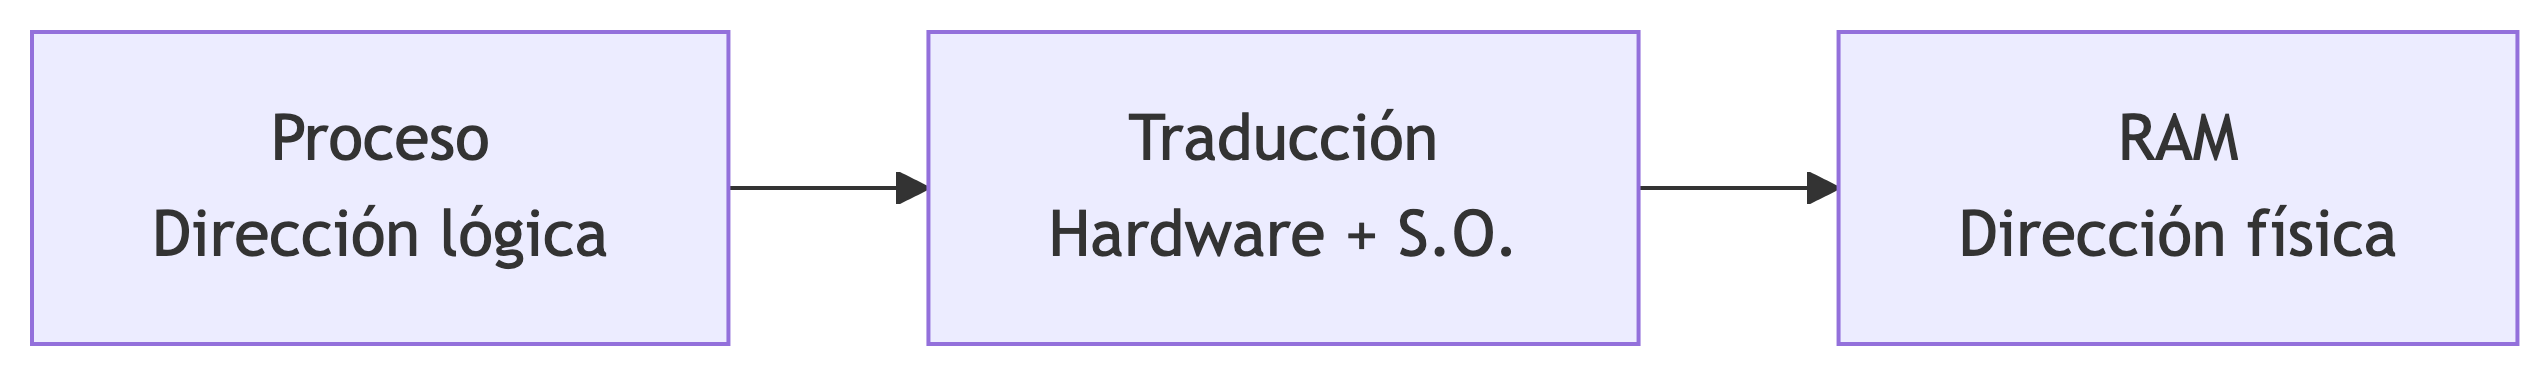
\includegraphics[width=7in,height=3.7in]{capitulos/13_manejo_memoria_paginacion_particiones_files/figure-latex/mermaid-figure-5.png}

\begin{tcolorbox}[enhanced jigsaw, arc=.35mm, bottomrule=.15mm, bottomtitle=1mm, breakable, colback=white, colbacktitle=quarto-callout-important-color!10!white, colframe=quarto-callout-important-color-frame, coltitle=black, left=2mm, leftrule=.75mm, opacityback=0, opacitybacktitle=0.6, rightrule=.15mm, title=\textcolor{quarto-callout-important-color}{\faExclamation}\hspace{0.5em}{No debemos confundirlas}, titlerule=0mm, toprule=.15mm, toptitle=1mm]

El proceso puede pensar en una dirección dentro de \textbf{su propio
espacio de memoria}, mientras el hardware y el Sistema Operativo
determinan dónde se encuentra realmente esa información en la RAM.

\end{tcolorbox}

\begin{center}\rule{0.5\linewidth}{0.5pt}\end{center}

\bookmarksetup{startatroot}

\chapter{3. Primera estrategia: dividir la memoria en
particiones}\label{primera-estrategia-dividir-la-memoria-en-particiones}

Una forma sencilla de administrar memoria consiste en dividirla en
\textbf{bloques o particiones}.

Cada proceso ocupa una partición.

Existen dos enfoques principales:

\begin{Shaded}
\begin{Highlighting}[]
\NormalTok{PARTICIONES}
\NormalTok{   │}
\NormalTok{   ├── Fijas}
\NormalTok{   │}
\NormalTok{   └── Dinámicas}
\end{Highlighting}
\end{Shaded}

La diferencia parece pequeña, pero produce problemas de fragmentación
diferentes.

\begin{center}\rule{0.5\linewidth}{0.5pt}\end{center}

\bookmarksetup{startatroot}

\chapter{4. Particiones fijas}\label{particiones-fijas}

En las \textbf{particiones fijas}, la memoria se divide previamente en
bloques de tamaño definido.

Supongamos una memoria disponible de \textbf{8 MB}, dividida en cuatro
particiones de \textbf{2 MB}:

\begin{Shaded}
\begin{Highlighting}[]
\NormalTok{RAM}
\NormalTok{┌──────────────────┐}
\NormalTok{│ Partición 1: 2MB │}
\NormalTok{├──────────────────┤}
\NormalTok{│ Partición 2: 2MB │}
\NormalTok{├──────────────────┤}
\NormalTok{│ Partición 3: 2MB │}
\NormalTok{├──────────────────┤}
\NormalTok{│ Partición 4: 2MB │}
\NormalTok{└──────────────────┘}
\end{Highlighting}
\end{Shaded}

Ahora llegan tres procesos:

\begin{Shaded}
\begin{Highlighting}[]
\NormalTok{Proceso A = 1.2 MB}
\NormalTok{Proceso B = 1.8 MB}
\NormalTok{Proceso C = 0.9 MB}
\end{Highlighting}
\end{Shaded}

Podemos asignar uno a cada partición.

Pero observemos lo que ocurre:

{\def\LTcaptype{none} % do not increment counter
\begin{longtable}[]{@{}lrlrr@{}}
\toprule\noalign{}
Partición & Tamaño & Proceso & Utilizado & Desperdiciado \\
\midrule\noalign{}
\endhead
\bottomrule\noalign{}
\endlastfoot
1 & 2 MB & A & 1.2 MB & 0.8 MB \\
2 & 2 MB & B & 1.8 MB & 0.2 MB \\
3 & 2 MB & C & 0.9 MB & 1.1 MB \\
4 & 2 MB & Libre & --- & --- \\
\end{longtable}
}

Los espacios que sobran \textbf{dentro de una partición ocupada} no
pueden ser aprovechados fácilmente por otro proceso.

Eso se llama \textbf{fragmentación interna}.

\begin{tcolorbox}[enhanced jigsaw, arc=.35mm, bottomrule=.15mm, bottomtitle=1mm, breakable, colback=white, colbacktitle=quarto-callout-warning-color!10!white, colframe=quarto-callout-warning-color-frame, coltitle=black, left=2mm, leftrule=.75mm, opacityback=0, opacitybacktitle=0.6, rightrule=.15mm, title=\textcolor{quarto-callout-warning-color}{\faExclamationTriangle}\hspace{0.5em}{Fragmentación interna}, titlerule=0mm, toprule=.15mm, toptitle=1mm]

Existe memoria asignada a un proceso que realmente \textbf{no está
siendo utilizada}, pero permanece encerrada dentro del bloque asignado.

\end{tcolorbox}

\section{Ventaja principal}\label{ventaja-principal}

\begin{itemize}
\tightlist
\item
  Es un esquema sencillo de administrar.
\end{itemize}

\section{Problema principal}\label{problema-principal}

\begin{itemize}
\tightlist
\item
  Puede desperdiciar bastante memoria debido a la fragmentación interna.
\end{itemize}

\begin{center}\rule{0.5\linewidth}{0.5pt}\end{center}

\bookmarksetup{startatroot}

\chapter{5. Particiones dinámicas}\label{particiones-dinuxe1micas}

¿Y si en lugar de construir bloques rígidos permitimos que cada proceso
reciba aproximadamente el espacio que necesita?

Ese es el principio de las \textbf{particiones dinámicas}.

Supongamos:

\begin{Shaded}
\begin{Highlighting}[]
\NormalTok{RAM disponible = 16 MB}

\NormalTok{Proceso A = 4 MB}
\NormalTok{Proceso B = 6 MB}
\NormalTok{Proceso C = 2 MB}
\end{Highlighting}
\end{Shaded}

La memoria podría verse así:

\begin{Shaded}
\begin{Highlighting}[]
\NormalTok{┌──────────────────┐}
\NormalTok{│ Proceso A   4 MB │}
\NormalTok{├──────────────────┤}
\NormalTok{│ Proceso B   6 MB │}
\NormalTok{├──────────────────┤}
\NormalTok{│ Proceso C   2 MB │}
\NormalTok{├──────────────────┤}
\NormalTok{│ Libre       4 MB │}
\NormalTok{└──────────────────┘}
\end{Highlighting}
\end{Shaded}

Hasta aquí parece una solución excelente.

Pero los procesos terminan.

Imaginemos que \textbf{Proceso B finaliza}:

\begin{Shaded}
\begin{Highlighting}[]
\NormalTok{┌──────────────────┐}
\NormalTok{│ Proceso A   4 MB │}
\NormalTok{├──────────────────┤}
\NormalTok{│ LIBRE       6 MB │}
\NormalTok{├──────────────────┤}
\NormalTok{│ Proceso C   2 MB │}
\NormalTok{├──────────────────┤}
\NormalTok{│ LIBRE       4 MB │}
\NormalTok{└──────────────────┘}
\end{Highlighting}
\end{Shaded}

Ahora tenemos \textbf{10 MB libres}, pero están separados en dos huecos.

Esto introduce otro problema.

\begin{center}\rule{0.5\linewidth}{0.5pt}\end{center}

\bookmarksetup{startatroot}

\chapter{6. Fragmentación interna y
externa}\label{fragmentaciuxf3n-interna-y-externa}

Estos conceptos suelen confundirse.

\section{Fragmentación interna}\label{fragmentaciuxf3n-interna}

El desperdicio se encuentra \textbf{dentro del espacio asignado}.

\begin{Shaded}
\begin{Highlighting}[]
\NormalTok{Partición de 4 KB}
\NormalTok{┌────────────────────┐}
\NormalTok{│ Proceso: 3 KB      │}
\NormalTok{│                    │}
\NormalTok{│ Desperdicio: 1 KB  │ ← dentro}
\NormalTok{└────────────────────┘}
\end{Highlighting}
\end{Shaded}

\section{Fragmentación externa}\label{fragmentaciuxf3n-externa}

Existe suficiente memoria libre en total, pero se encuentra
\textbf{dispersa entre espacios ocupados}.

\begin{Shaded}
\begin{Highlighting}[]
\NormalTok{┌──────────────┐}
\NormalTok{│ Proceso A    │}
\NormalTok{├──────────────┤}
\NormalTok{│ Libre 2 MB   │}
\NormalTok{├──────────────┤}
\NormalTok{│ Proceso B    │}
\NormalTok{├──────────────┤}
\NormalTok{│ Libre 3 MB   │}
\NormalTok{├──────────────┤}
\NormalTok{│ Proceso C    │}
\NormalTok{├──────────────┤}
\NormalTok{│ Libre 1 MB   │}
\NormalTok{└──────────────┘}
\end{Highlighting}
\end{Shaded}

Tenemos:

\begin{Shaded}
\begin{Highlighting}[]
\NormalTok{2 + 3 + 1 = 6 MB libres}
\end{Highlighting}
\end{Shaded}

pero \textbf{no existe necesariamente un bloque contiguo de 6 MB}.

{\def\LTcaptype{none} % do not increment counter
\begin{longtable}[]{@{}
  >{\raggedright\arraybackslash}p{(\linewidth - 4\tabcolsep) * \real{0.3333}}
  >{\raggedright\arraybackslash}p{(\linewidth - 4\tabcolsep) * \real{0.3333}}
  >{\raggedright\arraybackslash}p{(\linewidth - 4\tabcolsep) * \real{0.3333}}@{}}
\toprule\noalign{}
\begin{minipage}[b]{\linewidth}\raggedright
Tipo
\end{minipage} & \begin{minipage}[b]{\linewidth}\raggedright
¿Dónde está el desperdicio?
\end{minipage} & \begin{minipage}[b]{\linewidth}\raggedright
Ejemplo típico
\end{minipage} \\
\midrule\noalign{}
\endhead
\bottomrule\noalign{}
\endlastfoot
\textbf{Interna} & Dentro del bloque asignado & Particiones fijas /
último marco de una página \\
\textbf{Externa} & Entre bloques ocupados & Particiones dinámicas \\
\end{longtable}
}

\begin{tcolorbox}[enhanced jigsaw, arc=.35mm, bottomrule=.15mm, bottomtitle=1mm, breakable, colback=white, colbacktitle=quarto-callout-tip-color!10!white, colframe=quarto-callout-tip-color-frame, coltitle=black, left=2mm, leftrule=.75mm, opacityback=0, opacitybacktitle=0.6, rightrule=.15mm, title=\textcolor{quarto-callout-tip-color}{\faLightbulb}\hspace{0.5em}{Truco para recordarlo}, titlerule=0mm, toprule=.15mm, toptitle=1mm]

\textbf{Interna → adentro del bloque.}\\
\textbf{Externa → afuera, entre los bloques.}

\end{tcolorbox}

\begin{center}\rule{0.5\linewidth}{0.5pt}\end{center}

\bookmarksetup{startatroot}

\chapter{7. ¿Qué hueco debemos
utilizar?}\label{quuxe9-hueco-debemos-utilizar}

Con particiones dinámicas aparece otra pregunta:

\begin{quote}
Si existen varios espacios libres, ¿en cuál colocamos el nuevo proceso?
\end{quote}

Tres estrategias clásicas son:

\begin{itemize}
\tightlist
\item
  \textbf{First Fit}
\item
  \textbf{Best Fit}
\item
  \textbf{Worst Fit}
\end{itemize}

Supongamos que tenemos estos huecos:

\begin{Shaded}
\begin{Highlighting}[]
\NormalTok{10 KB   4 KB   20 KB   7 KB}
\end{Highlighting}
\end{Shaded}

y llega un proceso de:

\begin{Shaded}
\begin{Highlighting}[]
\NormalTok{6 KB}
\end{Highlighting}
\end{Shaded}

\begin{center}\rule{0.5\linewidth}{0.5pt}\end{center}

\bookmarksetup{startatroot}

\chapter{8. First Fit: el primer espacio
suficiente}\label{first-fit-el-primer-espacio-suficiente}

\textbf{First Fit} recorre la memoria y selecciona el \textbf{primer
hueco que sea suficientemente grande}.

Para nuestro proceso de 6 KB:

\begin{Shaded}
\begin{Highlighting}[]
\NormalTok{Huecos: 10 KB | 4 KB | 20 KB | 7 KB}
\NormalTok{          ↑}
\NormalTok{       elegido}
\end{Highlighting}
\end{Shaded}

El primer hueco de 10 KB puede alojarlo.

Quedan:

\begin{Shaded}
\begin{Highlighting}[]
\NormalTok{10 {-} 6 = 4 KB}
\end{Highlighting}
\end{Shaded}

\begin{tcolorbox}[enhanced jigsaw, arc=.35mm, bottomrule=.15mm, bottomtitle=1mm, breakable, colback=white, colbacktitle=quarto-callout-note-color!10!white, colframe=quarto-callout-note-color-frame, coltitle=black, left=2mm, leftrule=.75mm, opacityback=0, opacitybacktitle=0.6, rightrule=.15mm, title=\textcolor{quarto-callout-note-color}{\faInfo}\hspace{0.5em}{Idea de First Fit}, titlerule=0mm, toprule=.15mm, toptitle=1mm]

No busca el hueco perfecto. Busca \textbf{el primero que funcione}.

\end{tcolorbox}

\begin{center}\rule{0.5\linewidth}{0.5pt}\end{center}

\bookmarksetup{startatroot}

\chapter{9. Best Fit: el espacio más
ajustado}\label{best-fit-el-espacio-muxe1s-ajustado}

\textbf{Best Fit} busca el hueco disponible más pequeño que todavía
pueda alojar el proceso.

\begin{Shaded}
\begin{Highlighting}[]
\NormalTok{Huecos: 10 KB | 4 KB | 20 KB | 7 KB}
\NormalTok{                                  ↑}
\NormalTok{                               elegido}
\end{Highlighting}
\end{Shaded}

Para un proceso de 6 KB, el hueco de 7 KB es el más ajustado.

Queda:

\begin{Shaded}
\begin{Highlighting}[]
\NormalTok{7 {-} 6 = 1 KB}
\end{Highlighting}
\end{Shaded}

La idea parece eficiente porque deja poco sobrante en esa asignación,
aunque puede producir huecos pequeños difíciles de reutilizar.

\begin{center}\rule{0.5\linewidth}{0.5pt}\end{center}

\bookmarksetup{startatroot}

\chapter{10. Worst Fit: el espacio más
grande}\label{worst-fit-el-espacio-muxe1s-grande}

\textbf{Worst Fit} hace lo contrario: selecciona el hueco más grande.

\begin{Shaded}
\begin{Highlighting}[]
\NormalTok{Huecos: 10 KB | 4 KB | 20 KB | 7 KB}
\NormalTok{                         ↑}
\NormalTok{                      elegido}
\end{Highlighting}
\end{Shaded}

El proceso de 6 KB entra en el hueco de 20 KB.

Quedan:

\begin{Shaded}
\begin{Highlighting}[]
\NormalTok{20 {-} 6 = 14 KB}
\end{Highlighting}
\end{Shaded}

La intención es conservar un espacio sobrante suficientemente grande
para ser útil posteriormente.

\begin{center}\rule{0.5\linewidth}{0.5pt}\end{center}

\bookmarksetup{startatroot}

\chapter{11. Comparando los tres
métodos}\label{comparando-los-tres-muxe9todos}

Para:

\begin{Shaded}
\begin{Highlighting}[]
\NormalTok{Huecos = 10, 4, 20, 7 KB}
\NormalTok{Proceso = 6 KB}
\end{Highlighting}
\end{Shaded}

{\def\LTcaptype{none} % do not increment counter
\begin{longtable}[]{@{}lrr@{}}
\toprule\noalign{}
Método & Hueco elegido & Espacio restante \\
\midrule\noalign{}
\endhead
\bottomrule\noalign{}
\endlastfoot
First Fit & 10 KB & 4 KB \\
Best Fit & 7 KB & 1 KB \\
Worst Fit & 20 KB & 14 KB \\
\end{longtable}
}

\begin{tcolorbox}[enhanced jigsaw, arc=.35mm, bottomrule=.15mm, bottomtitle=1mm, breakable, colback=white, colbacktitle=quarto-callout-important-color!10!white, colframe=quarto-callout-important-color-frame, coltitle=black, left=2mm, leftrule=.75mm, opacityback=0, opacitybacktitle=0.6, rightrule=.15mm, title=\textcolor{quarto-callout-important-color}{\faExclamation}\hspace{0.5em}{No existe magia}, titlerule=0mm, toprule=.15mm, toptitle=1mm]

Estos algoritmos toman decisiones distintas sobre el mismo estado de
memoria. La elección puede influir en cómo quedan distribuidos los
huecos para futuras solicitudes.

\end{tcolorbox}

\section{Actividad rápida}\label{actividad-ruxe1pida}

Tenemos:

\begin{Shaded}
\begin{Highlighting}[]
\NormalTok{Huecos libres: 5 KB, 12 KB, 8 KB, 20 KB}
\NormalTok{Proceso nuevo: 7 KB}
\end{Highlighting}
\end{Shaded}

Determina qué hueco seleccionaría:

\begin{enumerate}
\def\labelenumi{\arabic{enumi}.}
\tightlist
\item
  First Fit.
\item
  Best Fit.
\item
  Worst Fit.
\end{enumerate}

\begin{tcolorbox}[enhanced jigsaw, arc=.35mm, bottomrule=.15mm, bottomtitle=1mm, breakable, colback=white, colbacktitle=quarto-callout-tip-color!10!white, colframe=quarto-callout-tip-color-frame, coltitle=black, left=2mm, leftrule=.75mm, opacityback=0, opacitybacktitle=0.6, rightrule=.15mm, title=\textcolor{quarto-callout-tip-color}{\faLightbulb}\hspace{0.5em}{✅ Solución propuesta}, titlerule=0mm, toprule=.15mm, toptitle=1mm]

\begin{itemize}
\tightlist
\item
  \textbf{First Fit:} 12 KB, porque es el primer hueco suficientemente
  grande.
\item
  \textbf{Best Fit:} 8 KB, porque es el hueco válido más pequeño.
\item
  \textbf{Worst Fit:} 20 KB, porque es el hueco más grande.
\end{itemize}

Después de colocar un proceso de 7 KB quedarían, respectivamente:

\begin{itemize}
\tightlist
\item
  First Fit → 5 KB libres en ese hueco.
\item
  Best Fit → 1 KB libre.
\item
  Worst Fit → 13 KB libres.
\end{itemize}

\end{tcolorbox}

\begin{center}\rule{0.5\linewidth}{0.5pt}\end{center}

\bookmarksetup{startatroot}

\chapter{12. El problema de exigir memoria
contigua}\label{el-problema-de-exigir-memoria-contigua}

Las particiones tienen una limitación importante: un proceso necesita
tradicionalmente un bloque continuo de memoria.

Supongamos:

\begin{Shaded}
\begin{Highlighting}[]
\NormalTok{Libre total = 12 KB}
\end{Highlighting}
\end{Shaded}

pero distribuido así:

\begin{Shaded}
\begin{Highlighting}[]
\NormalTok{4 KB + 3 KB + 5 KB}
\end{Highlighting}
\end{Shaded}

Un proceso de \textbf{10 KB} no cabe en ninguno de los huecos
individualmente.

Entonces surge una idea poderosa:

\begin{quote}
\textbf{¿Y si dividimos el proceso en pequeñas partes y permitimos
colocarlas en distintos lugares de la RAM?}
\end{quote}

Esa idea nos lleva a la \textbf{paginación}.

\begin{center}\rule{0.5\linewidth}{0.5pt}\end{center}

\bookmarksetup{startatroot}

\chapter{13. Introducción a la
paginación}\label{introducciuxf3n-a-la-paginaciuxf3n}

La paginación divide:

\begin{itemize}
\tightlist
\item
  el espacio lógico del proceso en \textbf{páginas};
\item
  la memoria física en \textbf{marcos}.
\end{itemize}

Y ambos tienen el \textbf{mismo tamaño}.

\begin{Shaded}
\begin{Highlighting}[]
\NormalTok{PROCESO                     RAM}
\NormalTok{┌──────────┐               ┌──────────┐}
\NormalTok{│ Página 0 │               │ Marco 0  │}
\NormalTok{├──────────┤               ├──────────┤}
\NormalTok{│ Página 1 │               │ Marco 1  │}
\NormalTok{├──────────┤               ├──────────┤}
\NormalTok{│ Página 2 │               │ Marco 2  │}
\NormalTok{├──────────┤               ├──────────┤}
\NormalTok{│ Página 3 │               │ Marco 3  │}
\NormalTok{└──────────┘               ├──────────┤}
\NormalTok{                           │ Marco 4  │}
\NormalTok{                           └──────────┘}
\end{Highlighting}
\end{Shaded}

\begin{tcolorbox}[enhanced jigsaw, arc=.35mm, bottomrule=.15mm, bottomtitle=1mm, breakable, colback=white, colbacktitle=quarto-callout-tip-color!10!white, colframe=quarto-callout-tip-color-frame, coltitle=black, left=2mm, leftrule=.75mm, opacityback=0, opacitybacktitle=0.6, rightrule=.15mm, title=\textcolor{quarto-callout-tip-color}{\faLightbulb}\hspace{0.5em}{Dos palabras fundamentales}, titlerule=0mm, toprule=.15mm, toptitle=1mm]

\textbf{Página = unidad lógica del proceso.}\\
\textbf{Marco = unidad física de la RAM.}

\end{tcolorbox}

\begin{center}\rule{0.5\linewidth}{0.5pt}\end{center}

\bookmarksetup{startatroot}

\chapter{14. La gran ventaja: memoria no
contigua}\label{la-gran-ventaja-memoria-no-contigua}

Supongamos un proceso de \textbf{4 páginas}.

No es necesario colocarlas juntas.

Podrían distribuirse así:

\begin{Shaded}
\begin{Highlighting}[]
\NormalTok{Página 0 → Marco 5}
\NormalTok{Página 1 → Marco 2}
\NormalTok{Página 2 → Marco 8}
\NormalTok{Página 3 → Marco 1}
\end{Highlighting}
\end{Shaded}

Visualmente:

\begin{Shaded}
\begin{Highlighting}[]
\NormalTok{PROCESO                    MEMORIA FÍSICA}
\NormalTok{P0 ─────────────────────→ M5}
\NormalTok{P1 ───────────────→       M2}
\NormalTok{P2 ─────────────────────→ M8}
\NormalTok{P3 ───────→               M1}
\end{Highlighting}
\end{Shaded}

Para el proceso, sus páginas forman parte de un mismo espacio lógico.

En la RAM, pueden encontrarse en lugares separados.

\begin{tcolorbox}[enhanced jigsaw, arc=.35mm, bottomrule=.15mm, bottomtitle=1mm, breakable, colback=white, colbacktitle=quarto-callout-important-color!10!white, colframe=quarto-callout-important-color-frame, coltitle=black, left=2mm, leftrule=.75mm, opacityback=0, opacitybacktitle=0.6, rightrule=.15mm, title=\textcolor{quarto-callout-important-color}{\faExclamation}\hspace{0.5em}{Aquí está el cambio de paradigma}, titlerule=0mm, toprule=.15mm, toptitle=1mm]

Con paginación, \textbf{un proceso ya no necesita ocupar un único bloque
físico contiguo de memoria}.

\end{tcolorbox}

\begin{center}\rule{0.5\linewidth}{0.5pt}\end{center}

\bookmarksetup{startatroot}

\chapter{15. Ejemplo numérico de
paginación}\label{ejemplo-numuxe9rico-de-paginaciuxf3n}

Tenemos un proceso de:

\begin{Shaded}
\begin{Highlighting}[]
\NormalTok{10 KB}
\end{Highlighting}
\end{Shaded}

y utilizamos páginas de:

\begin{Shaded}
\begin{Highlighting}[]
\NormalTok{1 KB}
\end{Highlighting}
\end{Shaded}

Entonces:

\begin{Shaded}
\begin{Highlighting}[]
\NormalTok{10 KB ÷ 1 KB = 10 páginas}
\end{Highlighting}
\end{Shaded}

El proceso tendrá:

\begin{Shaded}
\begin{Highlighting}[]
\NormalTok{P0, P1, P2, P3, P4, P5, P6, P7, P8, P9}
\end{Highlighting}
\end{Shaded}

La RAM también se divide en marcos de \textbf{1 KB}.

Cada página puede colocarse en cualquier marco disponible.

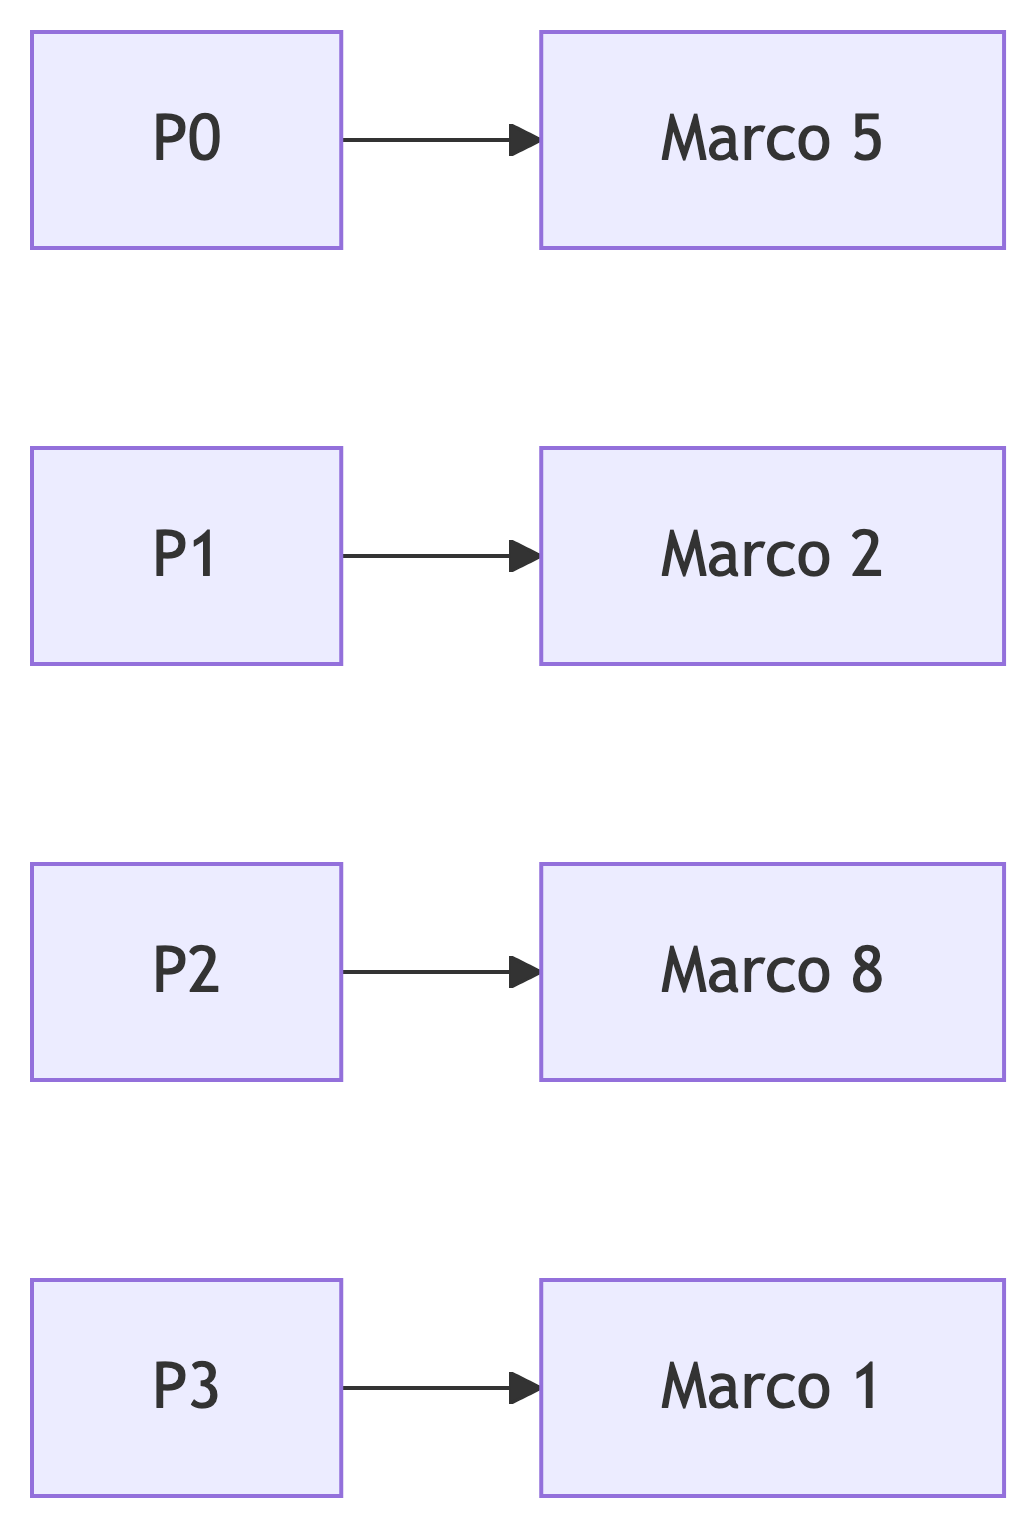
\includegraphics[width=7.2in,height=5.1in]{capitulos/13_manejo_memoria_paginacion_particiones_files/figure-latex/mermaid-figure-4.png}

El diagrama muestra solo algunas páginas para concentrarnos en el
mecanismo.

\begin{center}\rule{0.5\linewidth}{0.5pt}\end{center}

\bookmarksetup{startatroot}

\chapter{16. ¿Cómo sabe el Sistema Operativo dónde está cada
página?}\label{cuxf3mo-sabe-el-sistema-operativo-duxf3nde-estuxe1-cada-puxe1gina}

Necesitamos una estructura que mantenga la relación entre:

\begin{Shaded}
\begin{Highlighting}[]
\NormalTok{Página lógica ↔ Marco físico}
\end{Highlighting}
\end{Shaded}

Esa estructura es la \textbf{tabla de páginas}.

Ejemplo:

{\def\LTcaptype{none} % do not increment counter
\begin{longtable}[]{@{}rr@{}}
\toprule\noalign{}
Página & Marco \\
\midrule\noalign{}
\endhead
\bottomrule\noalign{}
\endlastfoot
0 & 5 \\
1 & 2 \\
2 & 8 \\
3 & 1 \\
\end{longtable}
}

Si el proceso solicita información de la \textbf{Página 2}, la tabla
indica:

\begin{Shaded}
\begin{Highlighting}[]
\NormalTok{Página 2 → Marco 8}
\end{Highlighting}
\end{Shaded}

\begin{tcolorbox}[enhanced jigsaw, arc=.35mm, bottomrule=.15mm, bottomtitle=1mm, breakable, colback=white, colbacktitle=quarto-callout-note-color!10!white, colframe=quarto-callout-note-color-frame, coltitle=black, left=2mm, leftrule=.75mm, opacityback=0, opacitybacktitle=0.6, rightrule=.15mm, title=\textcolor{quarto-callout-note-color}{\faInfo}\hspace{0.5em}{La tabla funciona como un mapa}, titlerule=0mm, toprule=.15mm, toptitle=1mm]

El proceso trabaja con páginas. La tabla de páginas permite encontrar el
\textbf{marco físico} donde se encuentra cada una.

\end{tcolorbox}

\begin{center}\rule{0.5\linewidth}{0.5pt}\end{center}

\bookmarksetup{startatroot}

\chapter{17. Dirección lógica = página +
desplazamiento}\label{direcciuxf3n-luxf3gica-puxe1gina-desplazamiento}

Una dirección lógica paginada puede pensarse como dos componentes:

\begin{Shaded}
\begin{Highlighting}[]
\NormalTok{┌────────────┬─────────────────┐}
\NormalTok{│   Página   │ Desplazamiento  │}
\NormalTok{└────────────┴─────────────────┘}
\end{Highlighting}
\end{Shaded}

La \textbf{página} indica qué página necesitamos.

El \textbf{desplazamiento} indica la posición dentro de esa página.

Supongamos:

\begin{Shaded}
\begin{Highlighting}[]
\NormalTok{Dirección lógica:}
\NormalTok{Página = 2}
\NormalTok{Desplazamiento = 100}
\end{Highlighting}
\end{Shaded}

La tabla contiene:

\begin{Shaded}
\begin{Highlighting}[]
\NormalTok{Página 2 → Marco 5}
\end{Highlighting}
\end{Shaded}

Entonces la dirección física será conceptualmente:

\begin{Shaded}
\begin{Highlighting}[]
\NormalTok{Marco = 5}
\NormalTok{Desplazamiento = 100}
\end{Highlighting}
\end{Shaded}

Observe algo importante:

\begin{quote}
\textbf{El desplazamiento no cambia.}
\end{quote}

Lo que cambia mediante la tabla es la página lógica por su marco físico
correspondiente.

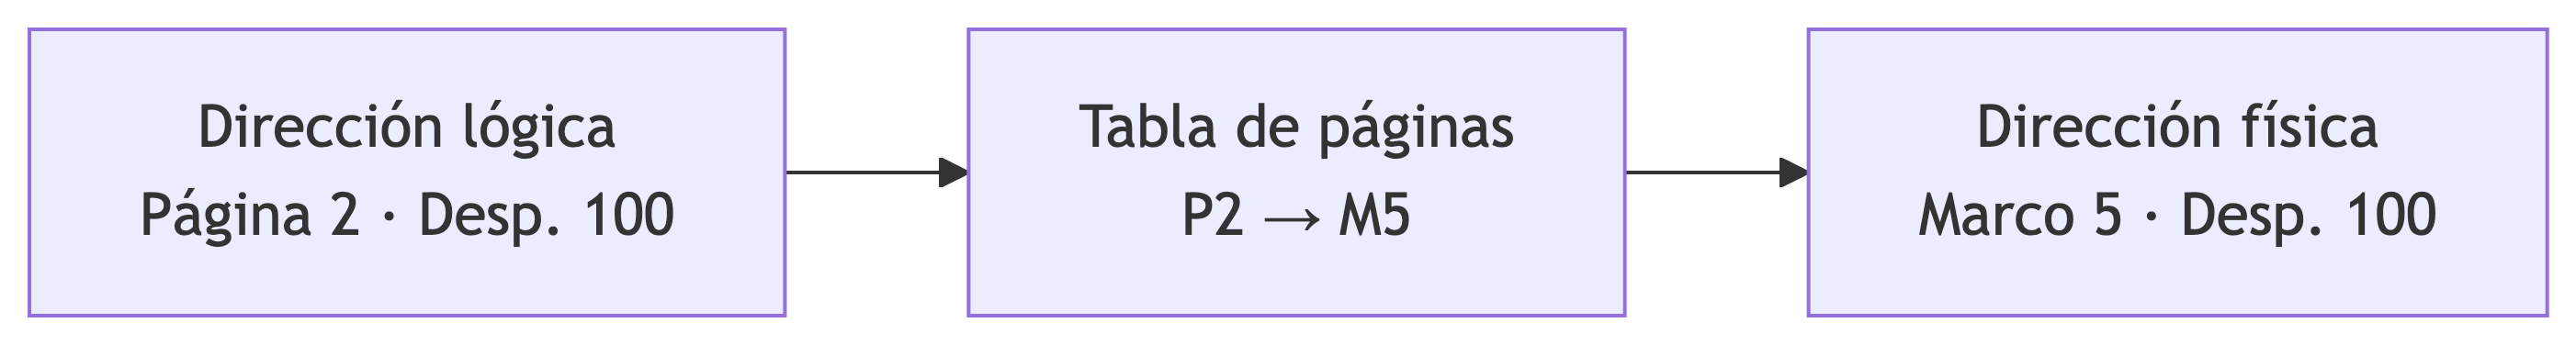
\includegraphics[width=7.4in,height=3.6in]{capitulos/13_manejo_memoria_paginacion_particiones_files/figure-latex/mermaid-figure-3.png}

\begin{center}\rule{0.5\linewidth}{0.5pt}\end{center}

\bookmarksetup{startatroot}

\chapter{18. Calculando una dirección
física}\label{calculando-una-direcciuxf3n-fuxedsica}

Podemos llevar el concepto un paso más adelante.

Si cada página y marco mide \textbf{1 KB}, entonces:

\begin{Shaded}
\begin{Highlighting}[]
\NormalTok{1 KB = 1024 bytes}
\end{Highlighting}
\end{Shaded}

Tenemos:

\begin{Shaded}
\begin{Highlighting}[]
\NormalTok{Página lógica = 2}
\NormalTok{Desplazamiento = 100}
\NormalTok{Página 2 → Marco 5}
\end{Highlighting}
\end{Shaded}

La dirección física numérica puede calcularse como:

\begin{Shaded}
\begin{Highlighting}[]
\NormalTok{Dirección física = (marco × tamaño del marco) + desplazamiento}
\end{Highlighting}
\end{Shaded}

Entonces:

\begin{Shaded}
\begin{Highlighting}[]
\NormalTok{Dirección física = (5 × 1024) + 100}
\NormalTok{                  = 5120 + 100}
\NormalTok{                  = 5220}
\end{Highlighting}
\end{Shaded}

Por lo tanto:

\begin{quote}
La dirección lógica \textbf{(Página 2, desplazamiento 100)} corresponde
a la dirección física \textbf{5220}.
\end{quote}

\begin{tcolorbox}[enhanced jigsaw, arc=.35mm, bottomrule=.15mm, bottomtitle=1mm, breakable, colback=white, colbacktitle=quarto-callout-warning-color!10!white, colframe=quarto-callout-warning-color-frame, coltitle=black, left=2mm, leftrule=.75mm, opacityback=0, opacitybacktitle=0.6, rightrule=.15mm, title=\textcolor{quarto-callout-warning-color}{\faExclamationTriangle}\hspace{0.5em}{No memorices sin comprender}, titlerule=0mm, toprule=.15mm, toptitle=1mm]

La fórmula tiene sentido porque primero llegamos al inicio del
\textbf{Marco 5} y luego avanzamos \textbf{100 bytes} dentro de él.

\end{tcolorbox}

\section{Practiquemos}\label{practiquemos-1}

Página de \textbf{1 KB}. La tabla indica:

\begin{Shaded}
\begin{Highlighting}[]
\NormalTok{Página 3 → Marco 7}
\end{Highlighting}
\end{Shaded}

La dirección lógica es:

\begin{Shaded}
\begin{Highlighting}[]
\NormalTok{Página = 3}
\NormalTok{Desplazamiento = 200}
\end{Highlighting}
\end{Shaded}

¿Cuál es la dirección física?

\begin{tcolorbox}[enhanced jigsaw, arc=.35mm, bottomrule=.15mm, bottomtitle=1mm, breakable, colback=white, colbacktitle=quarto-callout-tip-color!10!white, colframe=quarto-callout-tip-color-frame, coltitle=black, left=2mm, leftrule=.75mm, opacityback=0, opacitybacktitle=0.6, rightrule=.15mm, title=\textcolor{quarto-callout-tip-color}{\faLightbulb}\hspace{0.5em}{✅ Solución propuesta}, titlerule=0mm, toprule=.15mm, toptitle=1mm]

Como:

\begin{Shaded}
\begin{Highlighting}[]
\NormalTok{1 KB = 1024 bytes}
\end{Highlighting}
\end{Shaded}

y:

\begin{Shaded}
\begin{Highlighting}[]
\NormalTok{Página 3 → Marco 7}
\end{Highlighting}
\end{Shaded}

calculamos:

\begin{Shaded}
\begin{Highlighting}[]
\NormalTok{Dirección física = (7 × 1024) + 200}
\NormalTok{                  = 7168 + 200}
\NormalTok{                  = 7368}
\end{Highlighting}
\end{Shaded}

La dirección física es \textbf{7368}.

\end{tcolorbox}

\begin{center}\rule{0.5\linewidth}{0.5pt}\end{center}

\bookmarksetup{startatroot}

\chapter{19. ¿La paginación elimina toda
fragmentación?}\label{la-paginaciuxf3n-elimina-toda-fragmentaciuxf3n}

No.

La paginación evita el problema clásico de \textbf{fragmentación
externa}, porque las páginas pueden colocarse en marcos separados.

Sin embargo, todavía puede existir \textbf{fragmentación interna},
especialmente en el último marco utilizado por un proceso.

Ejemplo:

\begin{Shaded}
\begin{Highlighting}[]
\NormalTok{Proceso = 10 KB}
\NormalTok{Página  = 4 KB}
\end{Highlighting}
\end{Shaded}

Necesitamos:

\begin{Shaded}
\begin{Highlighting}[]
\NormalTok{Página 0 = 4 KB}
\NormalTok{Página 1 = 4 KB}
\NormalTok{Página 2 = 2 KB utilizados}
\end{Highlighting}
\end{Shaded}

Pero el último marco mide 4 KB.

\begin{Shaded}
\begin{Highlighting}[]
\NormalTok{Último marco:}
\NormalTok{┌──────────────────┐}
\NormalTok{│ 2 KB utilizados  │}
\NormalTok{├──────────────────┤}
\NormalTok{│ 2 KB sin utilizar│ ← fragmentación interna}
\NormalTok{└──────────────────┘}
\end{Highlighting}
\end{Shaded}

Por tanto:

\begin{Shaded}
\begin{Highlighting}[]
\NormalTok{Fragmentación interna = 2 KB}
\end{Highlighting}
\end{Shaded}

\begin{tcolorbox}[enhanced jigsaw, arc=.35mm, bottomrule=.15mm, bottomtitle=1mm, breakable, colback=white, colbacktitle=quarto-callout-important-color!10!white, colframe=quarto-callout-important-color-frame, coltitle=black, left=2mm, leftrule=.75mm, opacityback=0, opacitybacktitle=0.6, rightrule=.15mm, title=\textcolor{quarto-callout-important-color}{\faExclamation}\hspace{0.5em}{Una precisión importante}, titlerule=0mm, toprule=.15mm, toptitle=1mm]

La paginación \textbf{resuelve la necesidad de encontrar un gran bloque
contiguo}, pero no significa que todo byte de cada marco asignado será
aprovechado.

\end{tcolorbox}

\begin{center}\rule{0.5\linewidth}{0.5pt}\end{center}

\bookmarksetup{startatroot}

\chapter{20. Ventajas y costos de la
paginación}\label{ventajas-y-costos-de-la-paginaciuxf3n}

\section{Ventajas}\label{ventajas-10}

\begin{itemize}
\tightlist
\item
  Evita la fragmentación externa clásica.
\item
  Permite memoria física \textbf{no contigua}.
\item
  Facilita una utilización más flexible de los marcos disponibles.
\item
  Es una base importante para implementar \textbf{memoria virtual}.
\end{itemize}

\section{Costos o desventajas}\label{costos-o-desventajas}

\begin{itemize}
\tightlist
\item
  Puede existir fragmentación interna.
\item
  Cada proceso necesita información de traducción.
\item
  Las tablas de páginas consumen memoria.
\item
  La traducción de direcciones agrega trabajo al sistema.
\end{itemize}

{\def\LTcaptype{none} % do not increment counter
\begin{longtable}[]{@{}
  >{\raggedright\arraybackslash}p{(\linewidth - 2\tabcolsep) * \real{0.5000}}
  >{\raggedright\arraybackslash}p{(\linewidth - 2\tabcolsep) * \real{0.5000}}@{}}
\toprule\noalign{}
\begin{minipage}[b]{\linewidth}\raggedright
Particiones
\end{minipage} & \begin{minipage}[b]{\linewidth}\raggedright
Paginación
\end{minipage} \\
\midrule\noalign{}
\endhead
\bottomrule\noalign{}
\endlastfoot
Conceptualmente simples & Más flexible \\
Pueden requerir bloques contiguos & Permite marcos no contiguos \\
Dinámicas: fragmentación externa & Evita fragmentación externa
clásica \\
Fijas: fragmentación interna & Puede presentar fragmentación interna \\
Menor complejidad conceptual & Requiere tabla de páginas \\
\end{longtable}
}

\begin{center}\rule{0.5\linewidth}{0.5pt}\end{center}

\bookmarksetup{startatroot}

\chapter{21. De la paginación a la memoria
virtual}\label{de-la-paginaciuxf3n-a-la-memoria-virtual}

Hasta ahora hemos supuesto que las páginas del proceso están en RAM.

Pero aparece una posibilidad aún más interesante:

\begin{quote}
\textbf{¿Qué ocurre si un programa necesita más memoria de la que
podemos mantener físicamente en RAM en ese momento?}
\end{quote}

La \textbf{memoria virtual} permite extender el espacio disponible
utilizando almacenamiento secundario y mecanismos administrados por el
Sistema Operativo.

En un sistema paginado, algunas páginas pueden estar en RAM mientras
otras no se encuentran cargadas en ese instante.

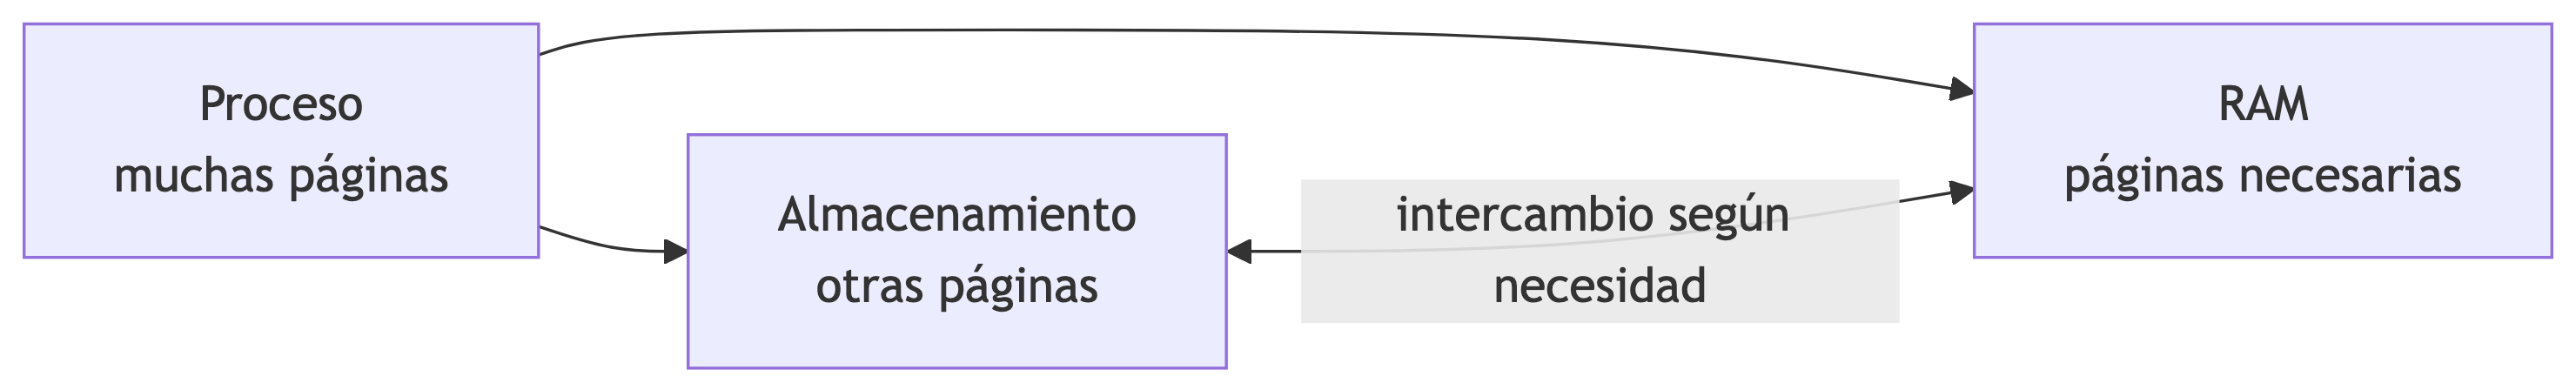
\includegraphics[width=7.4in,height=4.3in]{capitulos/13_manejo_memoria_paginacion_particiones_files/figure-latex/mermaid-figure-2.png}

\begin{tcolorbox}[enhanced jigsaw, arc=.35mm, bottomrule=.15mm, bottomtitle=1mm, breakable, colback=white, colbacktitle=quarto-callout-note-color!10!white, colframe=quarto-callout-note-color-frame, coltitle=black, left=2mm, leftrule=.75mm, opacityback=0, opacitybacktitle=0.6, rightrule=.15mm, title=\textcolor{quarto-callout-note-color}{\faInfo}\hspace{0.5em}{La idea que debemos conservar}, titlerule=0mm, toprule=.15mm, toptitle=1mm]

La memoria virtual permite que el espacio que observa un proceso no
tenga que corresponder completamente, en todo momento, con la cantidad
de RAM física que ocupa.

\end{tcolorbox}

\begin{center}\rule{0.5\linewidth}{0.5pt}\end{center}

\bookmarksetup{startatroot}

\chapter{22. Caso práctico
integrador}\label{caso-pruxe1ctico-integrador}

Tenemos una RAM disponible de \textbf{16 KB}.

Llegan tres procesos:

\begin{Shaded}
\begin{Highlighting}[]
\NormalTok{Proceso X = 4 KB}
\NormalTok{Proceso Y = 6 KB}
\NormalTok{Proceso Z = 2 KB}
\end{Highlighting}
\end{Shaded}

\section{Escenario A: particiones
dinámicas}\label{escenario-a-particiones-dinuxe1micas}

Inicialmente podrían almacenarse de forma contigua:

\begin{Shaded}
\begin{Highlighting}[]
\NormalTok{┌──────────────────┐}
\NormalTok{│ Proceso X   4 KB │}
\NormalTok{├──────────────────┤}
\NormalTok{│ Proceso Y   6 KB │}
\NormalTok{├──────────────────┤}
\NormalTok{│ Proceso Z   2 KB │}
\NormalTok{├──────────────────┤}
\NormalTok{│ Libre       4 KB │}
\NormalTok{└──────────────────┘}
\end{Highlighting}
\end{Shaded}

Si posteriormente termina el Proceso Y:

\begin{Shaded}
\begin{Highlighting}[]
\NormalTok{┌──────────────────┐}
\NormalTok{│ Proceso X   4 KB │}
\NormalTok{├──────────────────┤}
\NormalTok{│ Libre       6 KB │}
\NormalTok{├──────────────────┤}
\NormalTok{│ Proceso Z   2 KB │}
\NormalTok{├──────────────────┤}
\NormalTok{│ Libre       4 KB │}
\NormalTok{└──────────────────┘}
\end{Highlighting}
\end{Shaded}

Tenemos dos huecos separados.

\section{Escenario B: paginación de 2
KB}\label{escenario-b-paginaciuxf3n-de-2-kb}

La RAM de 16 KB contiene:

\begin{Shaded}
\begin{Highlighting}[]
\NormalTok{16 ÷ 2 = 8 marcos}
\end{Highlighting}
\end{Shaded}

Los procesos requieren:

\begin{Shaded}
\begin{Highlighting}[]
\NormalTok{X = 4 KB → 2 páginas}
\NormalTok{Y = 6 KB → 3 páginas}
\NormalTok{Z = 2 KB → 1 página}
\end{Highlighting}
\end{Shaded}

En total:

\begin{Shaded}
\begin{Highlighting}[]
\NormalTok{2 + 3 + 1 = 6 marcos utilizados}
\end{Highlighting}
\end{Shaded}

Las páginas podrían distribuirse, por ejemplo:

{\def\LTcaptype{none} % do not increment counter
\begin{longtable}[]{@{}lr@{}}
\toprule\noalign{}
Página & Marco \\
\midrule\noalign{}
\endhead
\bottomrule\noalign{}
\endlastfoot
X0 & 0 \\
Y0 & 1 \\
Z0 & 2 \\
X1 & 4 \\
Y1 & 6 \\
Y2 & 7 \\
\end{longtable}
}

No necesitan estar juntas.

\begin{tcolorbox}[enhanced jigsaw, arc=.35mm, bottomrule=.15mm, bottomtitle=1mm, breakable, colback=white, colbacktitle=quarto-callout-tip-color!10!white, colframe=quarto-callout-tip-color-frame, coltitle=black, left=2mm, leftrule=.75mm, opacityback=0, opacitybacktitle=0.6, rightrule=.15mm, title=\textcolor{quarto-callout-tip-color}{\faLightbulb}\hspace{0.5em}{Pregunta para discutir}, titlerule=0mm, toprule=.15mm, toptitle=1mm]

Si quedan libres los marcos 3 y 5, ¿representa eso el mismo problema que
dos huecos separados en particiones dinámicas?

\textbf{No necesariamente.} En paginación, un nuevo proceso puede
utilizar marcos libres separados porque sus páginas tampoco necesitan
quedar contiguas.

\end{tcolorbox}

\begin{center}\rule{0.5\linewidth}{0.5pt}\end{center}

\bookmarksetup{startatroot}

\chapter{23. Laboratorio en clase: tú administras la
RAM}\label{laboratorio-en-clase-tuxfa-administras-la-ram}

Supongamos una memoria de \textbf{32 KB}.

Existen estos huecos libres:

\begin{Shaded}
\begin{Highlighting}[]
\NormalTok{H1 = 8 KB}
\NormalTok{H2 = 5 KB}
\NormalTok{H3 = 12 KB}
\NormalTok{H4 = 7 KB}
\end{Highlighting}
\end{Shaded}

Llegan, en este orden:

\begin{Shaded}
\begin{Highlighting}[]
\NormalTok{Proceso A = 6 KB}
\NormalTok{Proceso B = 4 KB}
\NormalTok{Proceso C = 7 KB}
\end{Highlighting}
\end{Shaded}

\section{Parte A --- Particiones
dinámicas}\label{parte-a-particiones-dinuxe1micas}

Realiza la asignación utilizando por separado:

\begin{enumerate}
\def\labelenumi{\arabic{enumi}.}
\tightlist
\item
  First Fit.
\item
  Best Fit.
\item
  Worst Fit.
\end{enumerate}

Después de cada proceso, anota cómo quedan los huecos.

\section{Parte B --- Paginación}\label{parte-b-paginaciuxf3n}

Ahora supongamos páginas y marcos de \textbf{2 KB}.

Determina:

\begin{enumerate}
\def\labelenumi{\arabic{enumi}.}
\tightlist
\item
  cuántas páginas necesita cada proceso;
\item
  cuántos marcos necesita cada proceso;
\item
  si las páginas necesitan estar contiguas;
\item
  qué sucede con el Proceso B de 4 KB;
\item
  qué tipo de fragmentación puede existir.
\end{enumerate}

\section{Parte C --- Reflexión}\label{parte-c-reflexiuxf3n}

Responde:

\begin{quote}
¿Qué problema de las particiones dinámicas deja de ser crítico cuando
utilizamos paginación?
\end{quote}

\begin{tcolorbox}[enhanced jigsaw, arc=.35mm, bottomrule=.15mm, bottomtitle=1mm, breakable, colback=white, colbacktitle=quarto-callout-tip-color!10!white, colframe=quarto-callout-tip-color-frame, coltitle=black, left=2mm, leftrule=.75mm, opacityback=0, opacitybacktitle=0.6, rightrule=.15mm, title=\textcolor{quarto-callout-tip-color}{\faLightbulb}\hspace{0.5em}{✅ Solución propuesta}, titlerule=0mm, toprule=.15mm, toptitle=1mm]

\subsection{First Fit}\label{first-fit}

Huecos iniciales:

\begin{Shaded}
\begin{Highlighting}[]
\NormalTok{8, 5, 12, 7}
\end{Highlighting}
\end{Shaded}

Proceso A = 6 KB:

\begin{Shaded}
\begin{Highlighting}[]
\NormalTok{2, 5, 12, 7}
\end{Highlighting}
\end{Shaded}

Proceso B = 4 KB: el primer hueco suficiente es 5 KB.

\begin{Shaded}
\begin{Highlighting}[]
\NormalTok{2, 1, 12, 7}
\end{Highlighting}
\end{Shaded}

Proceso C = 7 KB: el primer hueco suficiente es 12 KB.

\begin{Shaded}
\begin{Highlighting}[]
\NormalTok{2, 1, 5, 7}
\end{Highlighting}
\end{Shaded}

\subsection{Best Fit}\label{best-fit}

Proceso A = 6 KB → utiliza 7 KB:

\begin{Shaded}
\begin{Highlighting}[]
\NormalTok{8, 5, 12, 1}
\end{Highlighting}
\end{Shaded}

Proceso B = 4 KB → utiliza 5 KB:

\begin{Shaded}
\begin{Highlighting}[]
\NormalTok{8, 1, 12, 1}
\end{Highlighting}
\end{Shaded}

Proceso C = 7 KB → utiliza 8 KB:

\begin{Shaded}
\begin{Highlighting}[]
\NormalTok{1, 1, 12, 1}
\end{Highlighting}
\end{Shaded}

\subsection{Worst Fit}\label{worst-fit}

Proceso A = 6 KB → utiliza 12 KB:

\begin{Shaded}
\begin{Highlighting}[]
\NormalTok{8, 5, 6, 7}
\end{Highlighting}
\end{Shaded}

Proceso B = 4 KB → utiliza 8 KB:

\begin{Shaded}
\begin{Highlighting}[]
\NormalTok{4, 5, 6, 7}
\end{Highlighting}
\end{Shaded}

Proceso C = 7 KB → utiliza 7 KB:

\begin{Shaded}
\begin{Highlighting}[]
\NormalTok{4, 5, 6, 0}
\end{Highlighting}
\end{Shaded}

\subsection{Paginación de 2 KB}\label{paginaciuxf3n-de-2-kb}

\begin{itemize}
\tightlist
\item
  Proceso A = 6 KB → \textbf{3 páginas / 3 marcos}.
\item
  Proceso B = 4 KB → \textbf{2 páginas / 2 marcos}.
\item
  Proceso C = 7 KB → necesita \textbf{4 páginas / 4 marcos}; la última
  página utiliza solo 1 KB.
\end{itemize}

Las páginas \textbf{no necesitan estar en marcos contiguos}.

En el Proceso C aparece hasta \textbf{1 KB de fragmentación interna} en
su último marco.

La paginación evita que los \textbf{huecos libres dispersos} impidan por
sí solos cargar un proceso, siempre que existan suficientes marcos
libres.

\end{tcolorbox}

\begin{center}\rule{0.5\linewidth}{0.5pt}\end{center}

\bookmarksetup{startatroot}

\chapter{24. Errores comunes}\label{errores-comunes}

\section{``Fragmentación interna y externa son lo
mismo''}\label{fragmentaciuxf3n-interna-y-externa-son-lo-mismo}

No.

\begin{itemize}
\tightlist
\item
  Interna → espacio desperdiciado \textbf{dentro} de una unidad
  asignada.
\item
  Externa → memoria libre \textbf{dispersa entre} unidades ocupadas.
\end{itemize}

\section{``Best Fit siempre es la mejor
estrategia''}\label{best-fit-siempre-es-la-mejor-estrategia}

El nombre puede engañar. Significa que selecciona el hueco más ajustado,
no que produzca necesariamente el mejor comportamiento en todas las
situaciones.

\section{``Las páginas deben quedar juntas en
RAM''}\label{las-puxe1ginas-deben-quedar-juntas-en-ram}

No.~Precisamente una de las ventajas fundamentales de la paginación es
permitir distribución \textbf{no contigua}.

\section{``Página y marco son
sinónimos''}\label{puxe1gina-y-marco-son-sinuxf3nimos}

Tienen el mismo tamaño dentro de un esquema paginado, pero representan
cosas distintas:

\begin{Shaded}
\begin{Highlighting}[]
\NormalTok{Página → espacio lógico}
\NormalTok{Marco  → memoria física}
\end{Highlighting}
\end{Shaded}

\section{``La paginación elimina toda
fragmentación''}\label{la-paginaciuxf3n-elimina-toda-fragmentaciuxf3n-1}

No.~Evita la fragmentación externa clásica, pero puede existir
\textbf{fragmentación interna}.

\begin{center}\rule{0.5\linewidth}{0.5pt}\end{center}

\bookmarksetup{startatroot}

\chapter{25. Autoevaluación}\label{autoevaluaciuxf3n-8}

\begin{enumerate}
\def\labelenumi{\arabic{enumi}.}
\tightlist
\item
  ¿Por qué la memoria es un recurso crítico?
\item
  ¿Qué funciones realiza el Sistema Operativo sobre la memoria?
\item
  ¿Qué diferencia existe entre dirección lógica y dirección física?
\item
  ¿Qué es una partición fija?
\item
  ¿Qué es una partición dinámica?
\item
  Explica con tus palabras la fragmentación interna.
\item
  Explica con tus palabras la fragmentación externa.
\item
  ¿Cómo funciona First Fit?
\item
  ¿Cómo funciona Best Fit?
\item
  ¿Cómo funciona Worst Fit?
\item
  ¿Qué problema aparece cuando existe suficiente memoria libre total,
  pero está dispersa?
\item
  ¿Qué es una página?
\item
  ¿Qué es un marco?
\item
  ¿Por qué página y marco deben tener el mismo tamaño?
\item
  ¿Qué función cumple la tabla de páginas?
\item
  ¿Qué elementos forman una dirección lógica paginada?
\item
  ¿Qué ocurre con el desplazamiento durante la traducción?
\item
  ¿Por qué la paginación permite memoria no contigua?
\item
  ¿Qué tipo de fragmentación puede aparecer en paginación?
\item
  ¿Cómo se relacionan paginación y memoria virtual?
\end{enumerate}

\begin{center}\rule{0.5\linewidth}{0.5pt}\end{center}

\bookmarksetup{startatroot}

\chapter{26. Reto final}\label{reto-final}

Un sistema utiliza páginas de \textbf{4 KB}.

Un proceso necesita \textbf{18 KB}.

Responde:

\begin{enumerate}
\def\labelenumi{\arabic{enumi}.}
\tightlist
\item
  ¿Cuántas páginas necesita?
\item
  ¿Cuántos marcos debe recibir?
\item
  ¿Cuánta memoria física se asignará en total?
\item
  ¿Cuánta fragmentación interna tendrá el último marco?
\item
  Si la Página 3 está en el Marco 9 y el desplazamiento es 500 bytes,
  ¿cuál es la dirección física?
\item
  ¿Las cinco páginas deben quedar en marcos consecutivos?
\end{enumerate}

\begin{tcolorbox}[enhanced jigsaw, arc=.35mm, bottomrule=.15mm, bottomtitle=1mm, breakable, colback=white, colbacktitle=quarto-callout-tip-color!10!white, colframe=quarto-callout-tip-color-frame, coltitle=black, left=2mm, leftrule=.75mm, opacityback=0, opacitybacktitle=0.6, rightrule=.15mm, title=\textcolor{quarto-callout-tip-color}{\faLightbulb}\hspace{0.5em}{✅ Solución propuesta}, titlerule=0mm, toprule=.15mm, toptitle=1mm]

\subsection{1. Número de páginas}\label{nuxfamero-de-puxe1ginas}

\begin{Shaded}
\begin{Highlighting}[]
\NormalTok{18 KB ÷ 4 KB = 4.5}
\end{Highlighting}
\end{Shaded}

Necesitamos \textbf{5 páginas}.

\subsection{2. Número de marcos}\label{nuxfamero-de-marcos}

Cada página necesita un marco, por lo que necesitamos \textbf{5 marcos}.

\subsection{3. Memoria física
asignada}\label{memoria-fuxedsica-asignada}

\begin{Shaded}
\begin{Highlighting}[]
\NormalTok{5 × 4 KB = 20 KB}
\end{Highlighting}
\end{Shaded}

\subsection{4. Fragmentación interna}\label{fragmentaciuxf3n-interna-1}

\begin{Shaded}
\begin{Highlighting}[]
\NormalTok{20 KB {-} 18 KB = 2 KB}
\end{Highlighting}
\end{Shaded}

La fragmentación interna es \textbf{2 KB}.

\subsection{5. Dirección física}\label{direcciuxf3n-fuxedsica}

Como:

\begin{Shaded}
\begin{Highlighting}[]
\NormalTok{4 KB = 4096 bytes}
\NormalTok{Marco = 9}
\NormalTok{Desplazamiento = 500}
\end{Highlighting}
\end{Shaded}

entonces:

\begin{Shaded}
\begin{Highlighting}[]
\NormalTok{Dirección física = (9 × 4096) + 500}
\NormalTok{                  = 36864 + 500}
\NormalTok{                  = 37364}
\end{Highlighting}
\end{Shaded}

La dirección física es \textbf{37364}.

\subsection{6. ¿Deben ser consecutivas?}\label{deben-ser-consecutivas}

\textbf{No.} Las páginas pueden almacenarse en marcos físicos no
contiguos.

\end{tcolorbox}

\begin{center}\rule{0.5\linewidth}{0.5pt}\end{center}

\bookmarksetup{startatroot}

\chapter{27. Para recordar}\label{para-recordar-4}

Podemos reconstruir el capítulo mediante esta secuencia:

\begin{Shaded}
\begin{Highlighting}[]
\NormalTok{RAM ES LIMITADA}
\NormalTok{      ↓}
\NormalTok{EL S.O. DEBE ADMINISTRARLA}
\NormalTok{      ↓}
\NormalTok{PARTICIONES}
\NormalTok{  ↓            ↓}
\NormalTok{FIJAS       DINÁMICAS}
\NormalTok{  ↓            ↓}
\NormalTok{Frag.       Frag.}
\NormalTok{interna     externa}
\NormalTok{      ↓}
\NormalTok{FIRST · BEST · WORST FIT}
\NormalTok{      ↓}
\NormalTok{¿Y SI NO EXIGIMOS CONTIGÜIDAD?}
\NormalTok{      ↓}
\NormalTok{PAGINACIÓN}
\NormalTok{      ↓}
\NormalTok{PÁGINAS ↔ TABLA ↔ MARCOS}
\NormalTok{      ↓}
\NormalTok{MEMORIA NO CONTIGUA}
\NormalTok{      ↓}
\NormalTok{MEMORIA VIRTUAL}
\end{Highlighting}
\end{Shaded}

\begin{tcolorbox}[enhanced jigsaw, arc=.35mm, bottomrule=.15mm, bottomtitle=1mm, breakable, colback=white, colbacktitle=quarto-callout-note-color!10!white, colframe=quarto-callout-note-color-frame, coltitle=black, left=2mm, leftrule=.75mm, opacityback=0, opacitybacktitle=0.6, rightrule=.15mm, title=\textcolor{quarto-callout-note-color}{\faInfo}\hspace{0.5em}{Síntesis en una frase}, titlerule=0mm, toprule=.15mm, toptitle=1mm]

\textbf{La paginación permite dividir un proceso en páginas y ubicarlas
en marcos físicos no contiguos, utilizando una tabla de páginas para
traducir direcciones lógicas en direcciones físicas.}

\end{tcolorbox}

\begin{center}\rule{0.5\linewidth}{0.5pt}\end{center}

\bookmarksetup{startatroot}

\chapter{Conexión con la siguiente
clase}\label{conexiuxf3n-con-la-siguiente-clase-2}

Ya comprendemos cómo el Sistema Operativo puede distribuir procesos en
memoria y cómo la paginación rompe la necesidad de mantener un proceso
completo en un bloque físico contiguo.

A partir de aquí podemos profundizar en mecanismos relacionados con
\textbf{memoria virtual}, carga de páginas bajo demanda y decisiones
sobre qué páginas deben permanecer en RAM.

\begin{center}\rule{0.5\linewidth}{0.5pt}\end{center}

\bookmarksetup{startatroot}

\chapter{Referencias}\label{referencias-1}

Material base de clase:

\begin{itemize}
\tightlist
\item
  Presentación \textbf{Manejo de memoria: Paginación y particiones},
  Sistemas Operativos I.
\end{itemize}

\begin{tcolorbox}[enhanced jigsaw, arc=.35mm, bottomrule=.15mm, bottomtitle=1mm, breakable, colback=white, colbacktitle=quarto-callout-tip-color!10!white, colframe=quarto-callout-tip-color-frame, coltitle=black, left=2mm, leftrule=.75mm, opacityback=0, opacitybacktitle=0.6, rightrule=.15mm, title=\textcolor{quarto-callout-tip-color}{\faLightbulb}\hspace{0.5em}{Criterio editorial}, titlerule=0mm, toprule=.15mm, toptitle=1mm]

Este capítulo transforma el material de clase en una secuencia de
razonamiento: \textbf{problema → estrategia → limitación → nueva
estrategia}. El objetivo no es memorizar términos, sino comprender por
qué surgieron las distintas técnicas de administración de memoria.

\end{tcolorbox}

\bookmarksetup{startatroot}

\chapter{Capítulo 14. Administración de memoria en
ejecución}\label{capuxedtulo-14.-administraciuxf3n-de-memoria-en-ejecuciuxf3n}

\bookmarksetup{startatroot}

\chapter{Capítulo 14. Administración de memoria en
ejecución}\label{capuxedtulo-14.-administraciuxf3n-de-memoria-en-ejecuciuxf3n-1}

\section{Del mapa de memoria a las decisiones del Sistema
Operativo}\label{del-mapa-de-memoria-a-las-decisiones-del-sistema-operativo}

En el capítulo anterior estudiamos \textbf{particiones, fragmentación,
algoritmos de ajuste y paginación}. Comprendimos cómo puede organizarse
la memoria y cómo una dirección lógica puede terminar asociada con una
ubicación física.

Ahora cambiaremos ligeramente la pregunta:

\begin{quote}
\textbf{Mientras los procesos están ejecutándose, ¿qué decisiones debe
tomar continuamente el Sistema Operativo para administrar la memoria?}
\end{quote}

La respuesta involucra asignación, protección, liberación, traducción de
direcciones, intercambio con disco, jerarquía de memoria y políticas de
reemplazo.

\begin{tcolorbox}[enhanced jigsaw, arc=.35mm, bottomrule=.15mm, bottomtitle=1mm, breakable, colback=white, colbacktitle=quarto-callout-tip-color!10!white, colframe=quarto-callout-tip-color-frame, coltitle=black, left=2mm, leftrule=.75mm, opacityback=0, opacitybacktitle=0.6, rightrule=.15mm, title=\textcolor{quarto-callout-tip-color}{\faLightbulb}\hspace{0.5em}{Idea central}, titlerule=0mm, toprule=.15mm, toptitle=1mm]

La administración de memoria no ocurre una sola vez cuando se inicia un
programa. Es un \textbf{proceso continuo} durante toda la vida de los
procesos.

\end{tcolorbox}

\begin{center}\rule{0.5\linewidth}{0.5pt}\end{center}

\bookmarksetup{startatroot}

\chapter{Objetivos de aprendizaje}\label{objetivos-de-aprendizaje-10}

Al finalizar este capítulo, el estudiante será capaz de:

\begin{itemize}
\tightlist
\item
  Explicar la función del administrador de memoria del Sistema
  Operativo.
\item
  Interpretar la \textbf{jerarquía de memoria} y su relación
  velocidad-capacidad-costo.
\item
  Relacionar direcciones lógicas y físicas con protección de memoria.
\item
  Explicar el uso conceptual de registros \textbf{base y límite}.
\item
  Interpretar un \textbf{mapa de memoria}.
\item
  Comprender el intercambio o \textbf{swapping} entre RAM y
  almacenamiento secundario.
\item
  Explicar por qué la compactación puede reducir fragmentación externa y
  cuál es su costo.
\item
  Relacionar caché, RAM y almacenamiento dentro de la jerarquía.
\item
  Introducir el propósito de las políticas de reemplazo, especialmente
  \textbf{LRU}.
\item
  Integrar estos mecanismos dentro del ciclo solicitud → asignación →
  ejecución → liberación.
\end{itemize}

\begin{center}\rule{0.5\linewidth}{0.5pt}\end{center}

\bookmarksetup{startatroot}

\chapter{1. ¿Qué administra realmente el Sistema
Operativo?}\label{quuxe9-administra-realmente-el-sistema-operativo}

La memoria principal es el espacio de trabajo inmediato de los procesos.
Mientras varios programas compiten por RAM, el Sistema Operativo debe
mantener control sobre cinco tareas esenciales:

\begin{enumerate}
\def\labelenumi{\arabic{enumi}.}
\tightlist
\item
  \textbf{Seguimiento:} saber qué zonas están ocupadas y cuáles libres.
\item
  \textbf{Asignación:} decidir dónde colocar la memoria solicitada por
  un proceso.
\item
  \textbf{Protección:} impedir que un proceso acceda indebidamente a
  otro.
\item
  \textbf{Intercambio:} mover temporalmente información entre RAM y
  almacenamiento cuando sea necesario.
\item
  \textbf{Liberación:} recuperar el espacio cuando deja de utilizarse.
\end{enumerate}

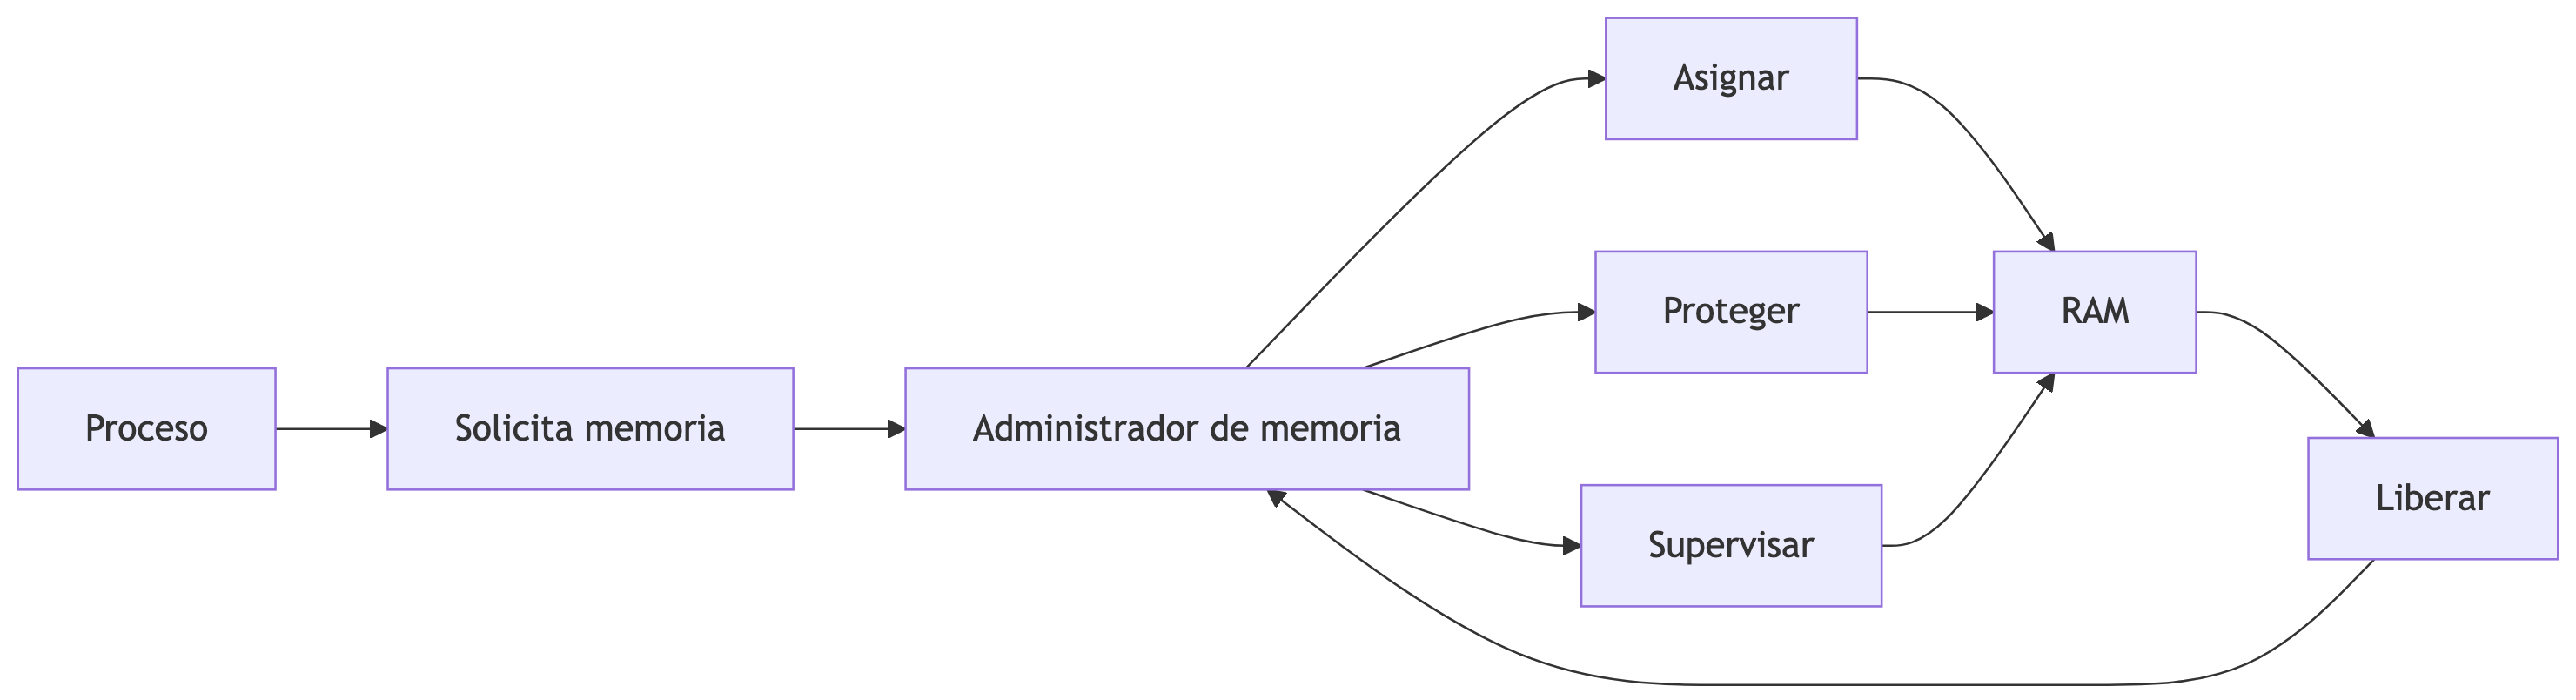
\includegraphics[width=7.4in,height=4.4in]{capitulos/14_administracion_memoria_en_ejecucion_files/figure-latex/mermaid-figure-1.png}

\begin{tcolorbox}[enhanced jigsaw, arc=.35mm, bottomrule=.15mm, bottomtitle=1mm, breakable, colback=white, colbacktitle=quarto-callout-note-color!10!white, colframe=quarto-callout-note-color-frame, coltitle=black, left=2mm, leftrule=.75mm, opacityback=0, opacitybacktitle=0.6, rightrule=.15mm, title=\textcolor{quarto-callout-note-color}{\faInfo}\hspace{0.5em}{Conexión con lo que ya sabemos}, titlerule=0mm, toprule=.15mm, toptitle=1mm]

Las particiones y la paginación estudiadas anteriormente son
\textbf{mecanismos de organización}. En esta clase observaremos el
trabajo operativo que existe alrededor de ellos.

\end{tcolorbox}

\begin{center}\rule{0.5\linewidth}{0.5pt}\end{center}

\bookmarksetup{startatroot}

\chapter{2. La jerarquía de memoria}\label{la-jerarquuxeda-de-memoria}

No toda la memoria de una computadora tiene la misma velocidad,
capacidad ni costo.

En términos generales:

{\def\LTcaptype{none} % do not increment counter
\begin{longtable}[]{@{}
  >{\raggedright\arraybackslash}p{(\linewidth - 8\tabcolsep) * \real{0.2000}}
  >{\raggedright\arraybackslash}p{(\linewidth - 8\tabcolsep) * \real{0.2000}}
  >{\raggedright\arraybackslash}p{(\linewidth - 8\tabcolsep) * \real{0.2000}}
  >{\raggedright\arraybackslash}p{(\linewidth - 8\tabcolsep) * \real{0.2000}}
  >{\raggedright\arraybackslash}p{(\linewidth - 8\tabcolsep) * \real{0.2000}}@{}}
\toprule\noalign{}
\begin{minipage}[b]{\linewidth}\raggedright
Nivel
\end{minipage} & \begin{minipage}[b]{\linewidth}\raggedright
Componente
\end{minipage} & \begin{minipage}[b]{\linewidth}\raggedright
Velocidad relativa
\end{minipage} & \begin{minipage}[b]{\linewidth}\raggedright
Capacidad relativa
\end{minipage} & \begin{minipage}[b]{\linewidth}\raggedright
Cercanía al CPU
\end{minipage} \\
\midrule\noalign{}
\endhead
\bottomrule\noalign{}
\endlastfoot
1 & Registros & Muy alta & Muy baja & Máxima \\
2 & Caché L1/L2/L3 & Alta & Baja & Muy cercana \\
3 & RAM & Media & Media & Intermedia \\
4 & SSD / almacenamiento & Mucho menor & Alta & Más lejana \\
\end{longtable}
}

\begin{center}
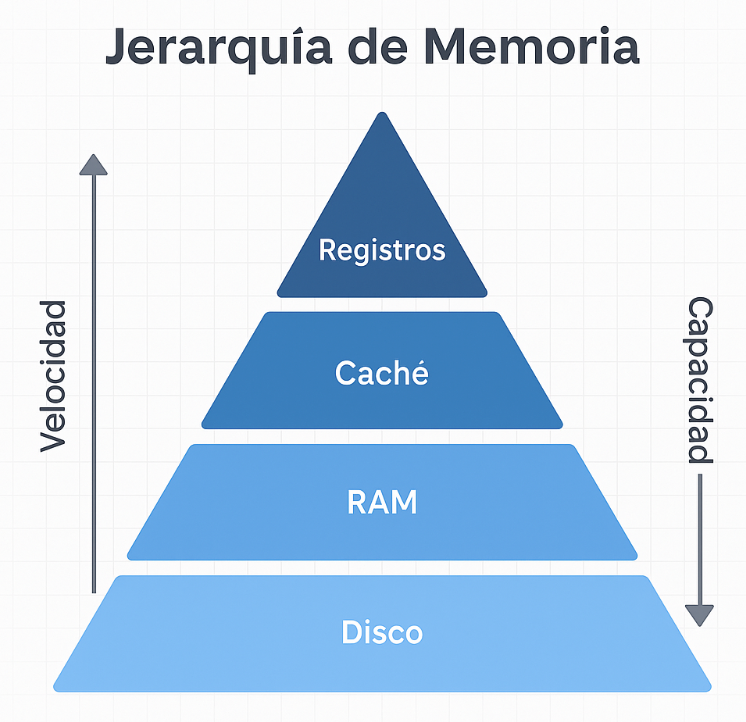
\includegraphics[width=0.72\linewidth,height=\textheight,keepaspectratio]{capitulos/img/capitulo14/14_jerarquia_memoria.png}
\end{center}

\begin{tcolorbox}[enhanced jigsaw, arc=.35mm, bottomrule=.15mm, bottomtitle=1mm, breakable, colback=white, colbacktitle=quarto-callout-important-color!10!white, colframe=quarto-callout-important-color-frame, coltitle=black, left=2mm, leftrule=.75mm, opacityback=0, opacitybacktitle=0.6, rightrule=.15mm, title=\textcolor{quarto-callout-important-color}{\faExclamation}\hspace{0.5em}{Una relación que conviene recordar}, titlerule=0mm, toprule=.15mm, toptitle=1mm]

Al acercarnos al CPU normalmente obtenemos \textbf{más velocidad y menos
capacidad}. Al alejarnos obtenemos \textbf{más capacidad, pero mayor
latencia}.

\end{tcolorbox}

\section{Una analogía sencilla}\label{una-analoguxeda-sencilla}

Pensemos en un estudiante resolviendo un ejercicio:

\begin{Shaded}
\begin{Highlighting}[]
\NormalTok{Dato que tiene en la mente       → Registro}
\NormalTok{Dato escrito en una hoja cercana → Caché}
\NormalTok{Libro abierto sobre el escritorio→ RAM}
\NormalTok{Libro guardado en la biblioteca  → Almacenamiento}
\end{Highlighting}
\end{Shaded}

Mientras más lejos esté la información, más tiempo necesitamos para
obtenerla.

\begin{center}\rule{0.5\linewidth}{0.5pt}\end{center}

\bookmarksetup{startatroot}

\chapter{3. ¿Por qué existe la
caché?}\label{por-quuxe9-existe-la-cachuxe9}

El CPU puede trabajar mucho más rápido que la RAM. Si tuviera que
esperar continuamente por cada dato, una parte importante de su
capacidad se desperdiciaría.

La \textbf{memoria caché} mantiene cerca del procesador datos e
instrucciones que probablemente serán utilizados nuevamente.

\begin{center}
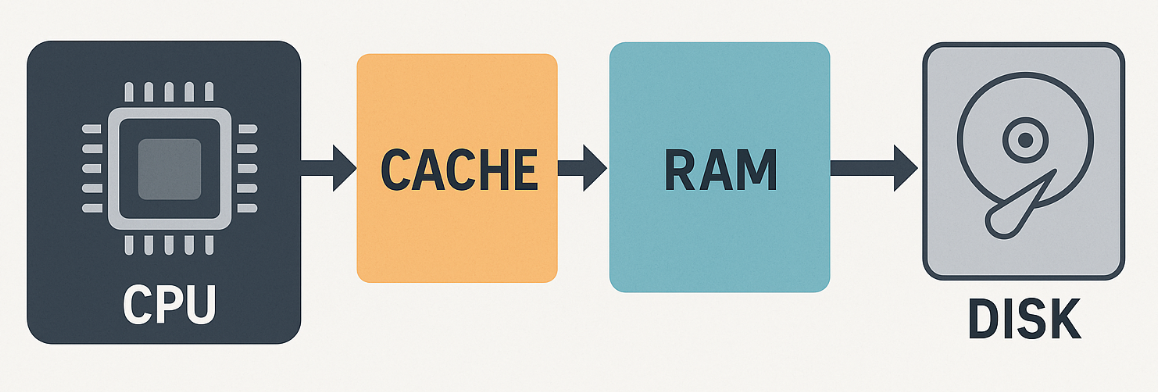
\includegraphics[width=0.68\linewidth,height=\textheight,keepaspectratio]{capitulos/img/capitulo14/14_cache.png}
\end{center}

Podemos resumir la idea:

\begin{Shaded}
\begin{Highlighting}[]
\NormalTok{CPU necesita un dato}
\NormalTok{       ↓}
\NormalTok{¿Está en caché?}
\NormalTok{   ↓ Sí       ↓ No}
\NormalTok{ usarlo      buscarlo en un nivel inferior}
\end{Highlighting}
\end{Shaded}

\begin{tcolorbox}[enhanced jigsaw, arc=.35mm, bottomrule=.15mm, bottomtitle=1mm, breakable, colback=white, colbacktitle=quarto-callout-note-color!10!white, colframe=quarto-callout-note-color-frame, coltitle=black, left=2mm, leftrule=.75mm, opacityback=0, opacitybacktitle=0.6, rightrule=.15mm, title=\textcolor{quarto-callout-note-color}{\faInfo}\hspace{0.5em}{No confundamos funciones}, titlerule=0mm, toprule=.15mm, toptitle=1mm]

La caché \textbf{no sustituye a la RAM} y la RAM no sustituye al
almacenamiento. Los niveles trabajan juntos para equilibrar velocidad,
capacidad y costo.

\end{tcolorbox}

\begin{center}\rule{0.5\linewidth}{0.5pt}\end{center}

\bookmarksetup{startatroot}

\chapter{4. Dirección lógica y dirección física: retomemos el
concepto}\label{direcciuxf3n-luxf3gica-y-direcciuxf3n-fuxedsica-retomemos-el-concepto}

En el capítulo anterior distinguimos:

\begin{itemize}
\tightlist
\item
  \textbf{dirección lógica:} la dirección utilizada dentro del espacio
  del proceso;
\item
  \textbf{dirección física:} la ubicación real correspondiente en RAM.
\end{itemize}

\begin{center}
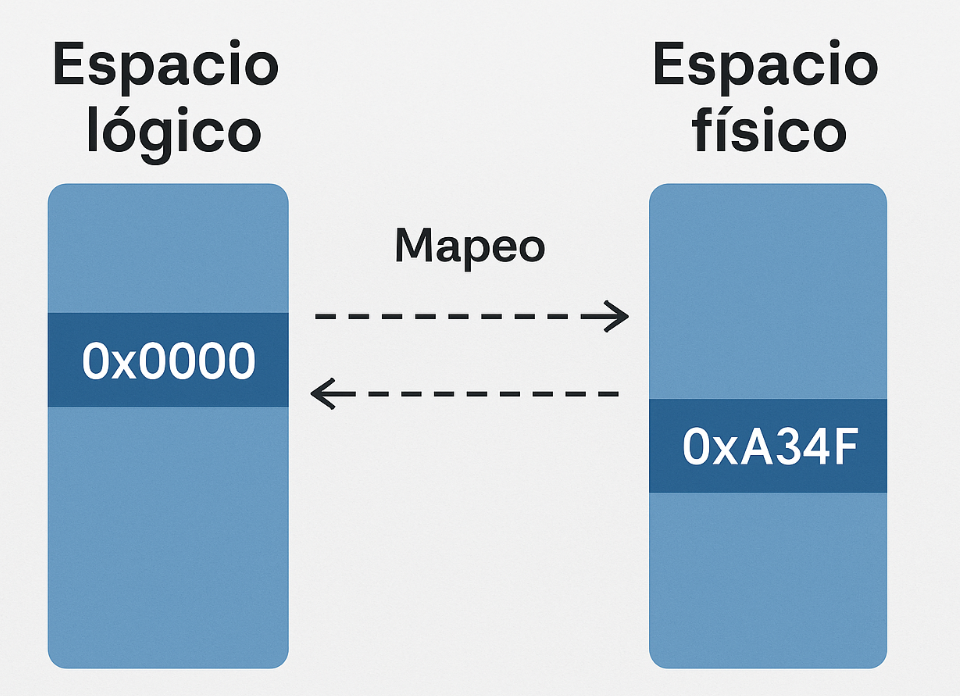
\includegraphics[width=0.7\linewidth,height=\textheight,keepaspectratio]{capitulos/img/capitulo14/14_logica_fisica.png}
\end{center}

La separación permite que un proceso no necesite conocer la ubicación
física exacta donde fue colocado.

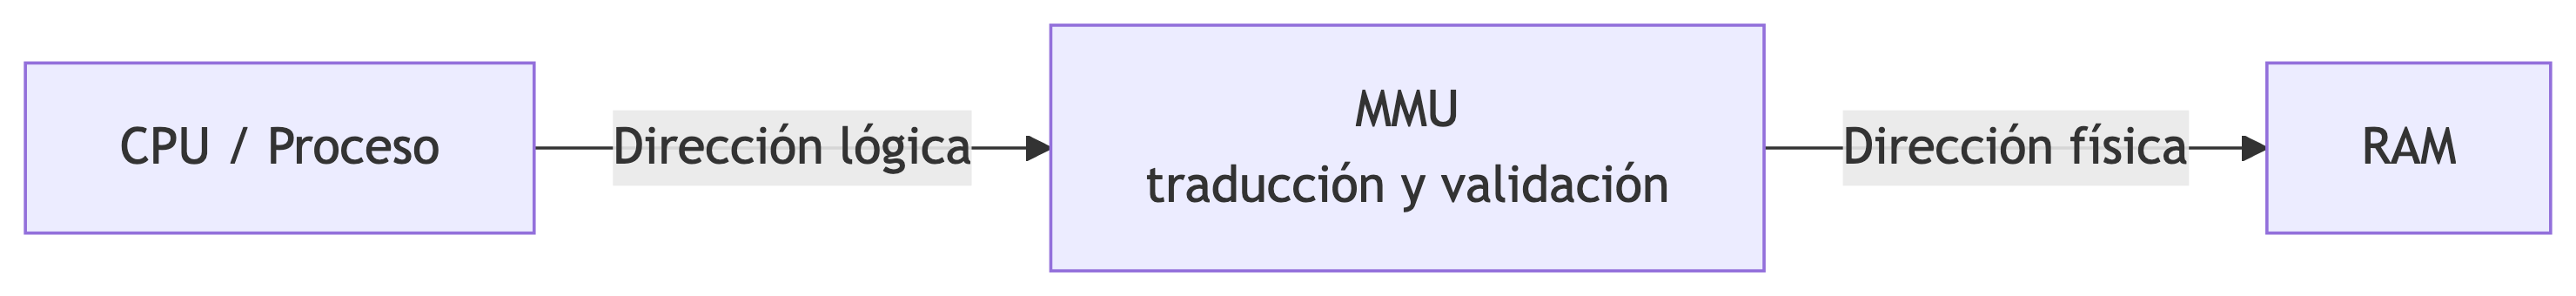
\includegraphics[width=7in,height=3.5in]{capitulos/14_administracion_memoria_en_ejecucion_files/figure-latex/mermaid-figure-4.png}

La \textbf{MMU (Memory Management Unit)} participa en la traducción y
comprobación de direcciones utilizando la información configurada por el
Sistema Operativo.

\begin{center}\rule{0.5\linewidth}{0.5pt}\end{center}

\bookmarksetup{startatroot}

\chapter{5. Protección de memoria}\label{protecciuxf3n-de-memoria}

Imaginemos dos procesos:

\begin{Shaded}
\begin{Highlighting}[]
\NormalTok{Proceso A → navegador}
\NormalTok{Proceso B → sistema de notas}
\end{Highlighting}
\end{Shaded}

¿Qué ocurriría si el navegador pudiera escribir libremente sobre la
memoria del sistema de notas?

Podría:

\begin{itemize}
\tightlist
\item
  alterar datos;
\item
  provocar errores;
\item
  comprometer información;
\item
  hacer fallar otros procesos o el sistema.
\end{itemize}

Por ello el Sistema Operativo y el hardware aplican mecanismos de
protección.

Entre los conceptos fundamentales encontramos:

\begin{itemize}
\tightlist
\item
  permisos de lectura;
\item
  permisos de escritura;
\item
  permisos de ejecución;
\item
  límites de regiones válidas;
\item
  excepciones cuando se intenta un acceso indebido.
\end{itemize}

\begin{tcolorbox}[enhanced jigsaw, arc=.35mm, bottomrule=.15mm, bottomtitle=1mm, breakable, colback=white, colbacktitle=quarto-callout-warning-color!10!white, colframe=quarto-callout-warning-color-frame, coltitle=black, left=2mm, leftrule=.75mm, opacityback=0, opacitybacktitle=0.6, rightrule=.15mm, title=\textcolor{quarto-callout-warning-color}{\faExclamationTriangle}\hspace{0.5em}{Idea fundamental}, titlerule=0mm, toprule=.15mm, toptitle=1mm]

La administración de memoria no busca solamente \textbf{aprovechar
espacio}. También debe garantizar \textbf{aislamiento y protección entre
procesos}.

\end{tcolorbox}

\begin{center}\rule{0.5\linewidth}{0.5pt}\end{center}

\bookmarksetup{startatroot}

\chapter{6. Registro base y límite}\label{registro-base-y-luxedmite}

Un modelo didáctico clásico para comprender protección y reubicación
utiliza dos valores:

\begin{itemize}
\tightlist
\item
  \textbf{Base:} inicio del espacio físico asignado.
\item
  \textbf{Límite:} tamaño máximo permitido para el proceso.
\end{itemize}

Supongamos:

\begin{Shaded}
\begin{Highlighting}[]
\NormalTok{Proceso A}
\NormalTok{Base   = 1000}
\NormalTok{Límite = 2000}
\end{Highlighting}
\end{Shaded}

El proceso dispone conceptualmente de desplazamientos desde \texttt{0}
hasta \texttt{1999}.

Si solicita:

\begin{Shaded}
\begin{Highlighting}[]
\NormalTok{Dirección lógica = 500}
\end{Highlighting}
\end{Shaded}

podemos representar:

\begin{Shaded}
\begin{Highlighting}[]
\NormalTok{Dirección física = Base + desplazamiento}
\NormalTok{                  = 1000 + 500}
\NormalTok{                  = 1500}
\end{Highlighting}
\end{Shaded}

Pero antes debemos comprobar:

\begin{Shaded}
\begin{Highlighting}[]
\NormalTok{¿500 \textless{} 2000?}
\end{Highlighting}
\end{Shaded}

Sí. El acceso se encuentra dentro del límite.

\section{¿Y si solicita 2300?}\label{y-si-solicita-2300}

\begin{Shaded}
\begin{Highlighting}[]
\NormalTok{2300 \textless{} 2000 → FALSO}
\end{Highlighting}
\end{Shaded}

El acceso debe rechazarse.

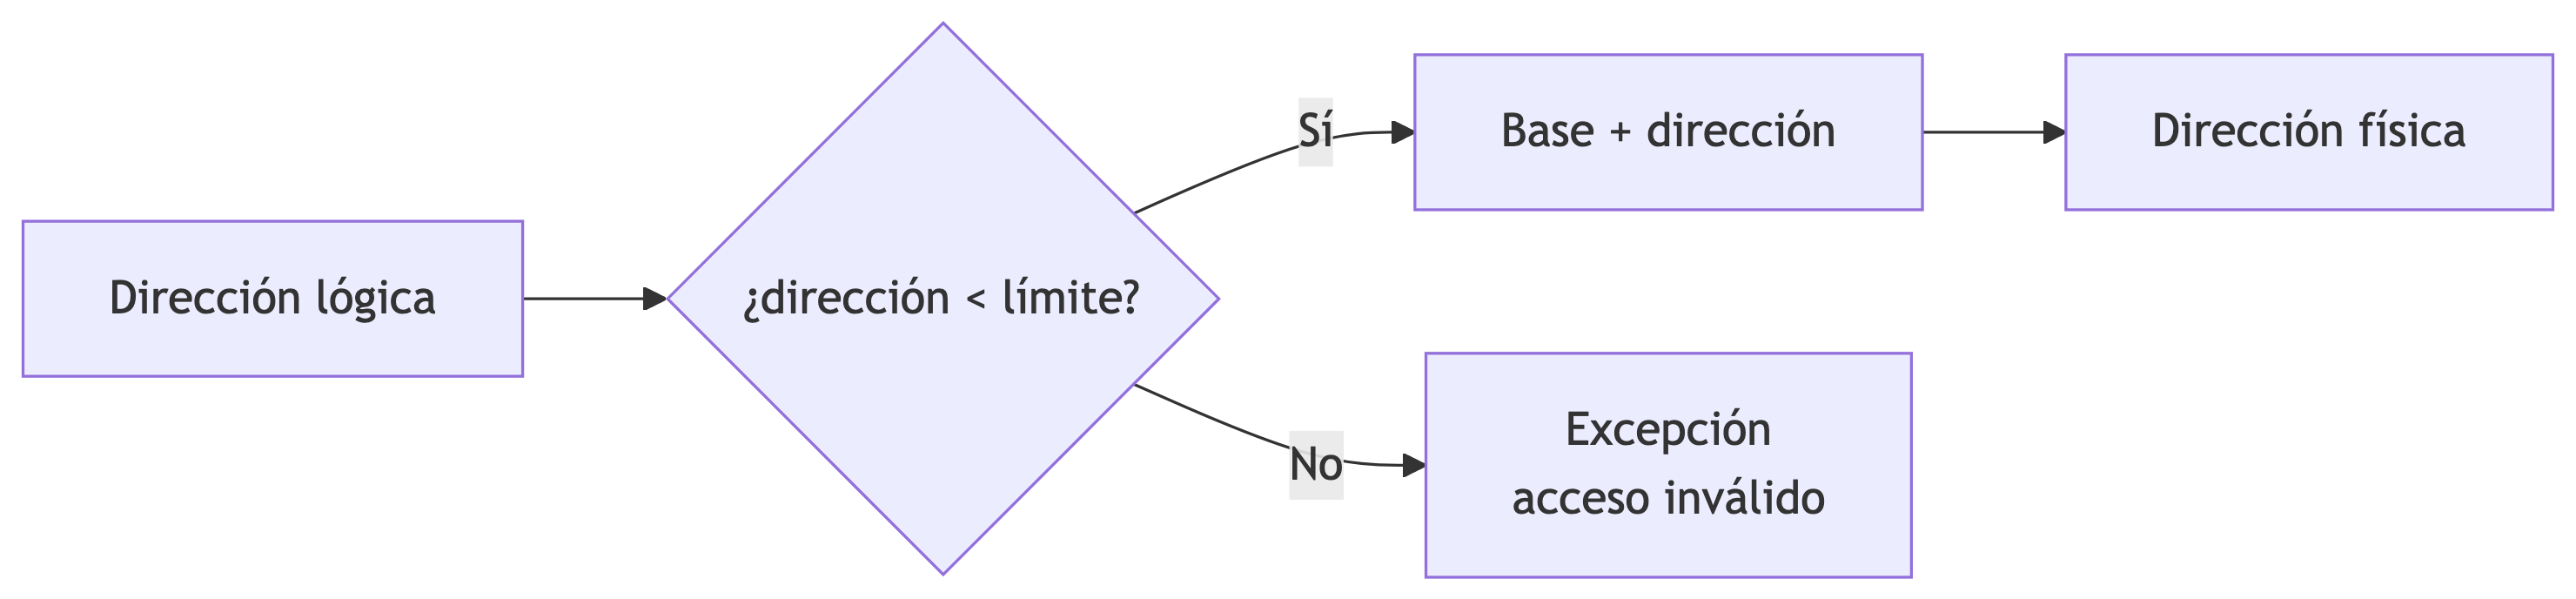
\includegraphics[width=7in,height=4in]{capitulos/14_administracion_memoria_en_ejecucion_files/figure-latex/mermaid-figure-3.png}

\begin{tcolorbox}[enhanced jigsaw, arc=.35mm, bottomrule=.15mm, bottomtitle=1mm, breakable, colback=white, colbacktitle=quarto-callout-tip-color!10!white, colframe=quarto-callout-tip-color-frame, coltitle=black, left=2mm, leftrule=.75mm, opacityback=0, opacitybacktitle=0.6, rightrule=.15mm, title=\textcolor{quarto-callout-tip-color}{\faLightbulb}\hspace{0.5em}{Pregunta para el grupo}, titlerule=0mm, toprule=.15mm, toptitle=1mm]

Si \texttt{Base\ =\ 4000}, \texttt{Límite\ =\ 1500} y el proceso
solicita la dirección lógica \texttt{1200}, ¿cuál sería la dirección
física? ¿El acceso es válido?

\end{tcolorbox}

\begin{center}\rule{0.5\linewidth}{0.5pt}\end{center}

\bookmarksetup{startatroot}

\chapter{7. Mapas de memoria: la fotografía de la
RAM}\label{mapas-de-memoria-la-fotografuxeda-de-la-ram}

Para administrar un recurso necesitamos saber qué parte se encuentra
disponible.

Un \textbf{mapa de memoria} representa regiones ocupadas y libres, y
puede asociarlas con procesos.

\begin{center}
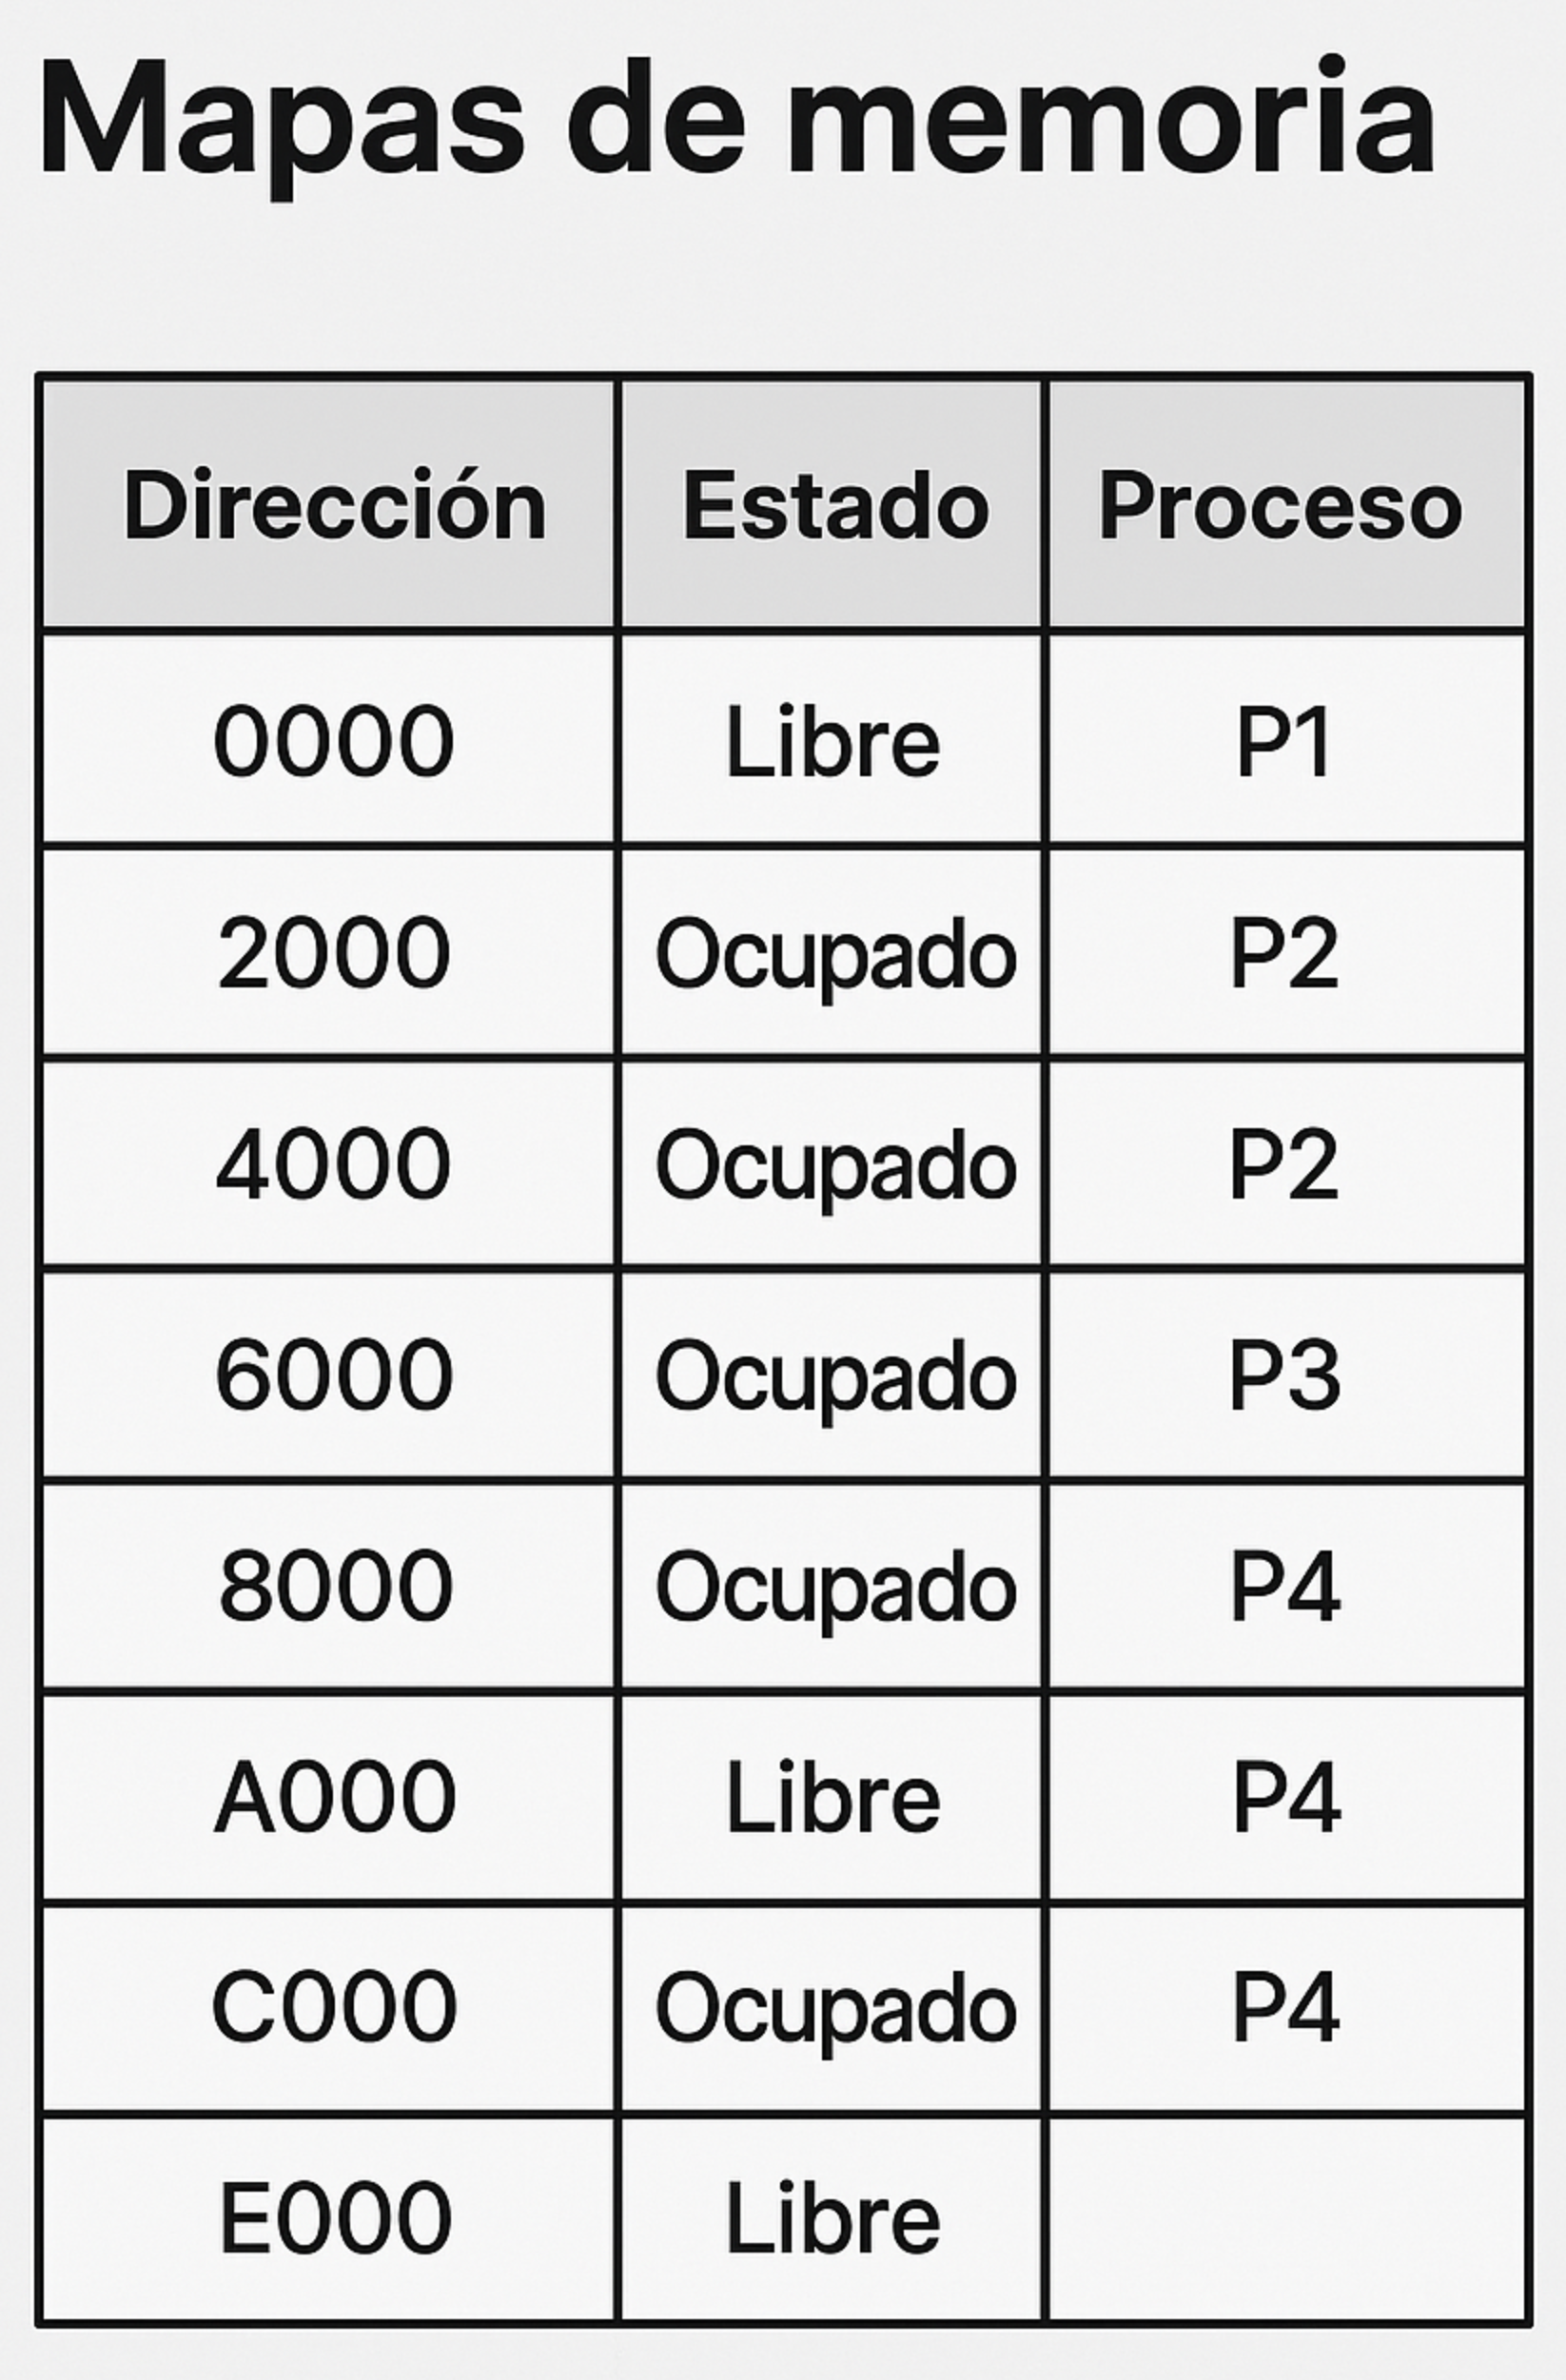
\includegraphics[width=0.67\linewidth,height=\textheight,keepaspectratio]{capitulos/img/capitulo14/14_mapa_memoria.png}
\end{center}

Una representación simplificada podría ser:

{\def\LTcaptype{none} % do not increment counter
\begin{longtable}[]{@{}rrll@{}}
\toprule\noalign{}
Inicio & Fin & Estado & Proceso \\
\midrule\noalign{}
\endhead
\bottomrule\noalign{}
\endlastfoot
0 & 199 & Ocupado & P1 \\
200 & 349 & Libre & --- \\
350 & 599 & Ocupado & P2 \\
600 & 799 & Libre & --- \\
\end{longtable}
}

Este mapa permite responder preguntas como:

\begin{itemize}
\tightlist
\item
  ¿cuánta memoria queda libre?;
\item
  ¿dónde existe un bloque disponible?;
\item
  ¿qué proceso ocupa determinada región?;
\item
  ¿qué ocurre cuando un proceso finaliza?;
\end{itemize}

\begin{center}\rule{0.5\linewidth}{0.5pt}\end{center}

\bookmarksetup{startatroot}

\chapter{8. Liberación: la memoria debe regresar al
sistema}\label{liberaciuxf3n-la-memoria-debe-regresar-al-sistema}

Asignar memoria es solamente la mitad del trabajo.

Cuando un proceso termina o deja de necesitar una región, el Sistema
Operativo debe marcar ese espacio como disponible.

\begin{Shaded}
\begin{Highlighting}[]
\NormalTok{ANTES}
\NormalTok{0        200        350        600}
\NormalTok{|{-}{-}{-}P1{-}{-}{-}|{-}{-}{-}P2{-}{-}{-}{-}{-}{-}|{-}{-}{-}Libre{-}{-}{-}|}

\NormalTok{P1 termina}

\NormalTok{DESPUÉS}
\NormalTok{0        200        350        600}
\NormalTok{|{-}{-}Libre{-}|{-}{-}{-}P2{-}{-}{-}{-}{-}{-}|{-}{-}{-}Libre{-}{-}{-}|}
\end{Highlighting}
\end{Shaded}

Ahora aparecen varios espacios libres separados.

Esto nos conecta con la \textbf{fragmentación externa} estudiada en el
capítulo anterior.

\begin{center}\rule{0.5\linewidth}{0.5pt}\end{center}

\bookmarksetup{startatroot}

\chapter{9. Compactación: reunir espacios
libres}\label{compactaciuxf3n-reunir-espacios-libres}

Cuando existen huecos libres dispersos, una estrategia conceptual
consiste en mover procesos para reunir esos espacios.

\begin{Shaded}
\begin{Highlighting}[]
\NormalTok{ANTES}
\NormalTok{[P1][Libre][P2][Libre][P3][Libre]}

\NormalTok{DESPUÉS}
\NormalTok{[P1][P2][P3][{-}{-}{-}{-}{-}{-}{-}{-}{-}Libre{-}{-}{-}{-}{-}]}
\end{Highlighting}
\end{Shaded}

A esto lo llamamos \textbf{compactación}.

\begin{tcolorbox}[enhanced jigsaw, arc=.35mm, bottomrule=.15mm, bottomtitle=1mm, breakable, colback=white, colbacktitle=quarto-callout-warning-color!10!white, colframe=quarto-callout-warning-color-frame, coltitle=black, left=2mm, leftrule=.75mm, opacityback=0, opacitybacktitle=0.6, rightrule=.15mm, title=\textcolor{quarto-callout-warning-color}{\faExclamationTriangle}\hspace{0.5em}{La compactación no es gratuita}, titlerule=0mm, toprule=.15mm, toptitle=1mm]

Mover procesos o regiones de memoria implica trabajo adicional. Por ello
la compactación ayuda a comprender el problema de la fragmentación
externa, pero tiene un \textbf{costo de tiempo y movimiento de datos}.

\end{tcolorbox}

\begin{center}\rule{0.5\linewidth}{0.5pt}\end{center}

\bookmarksetup{startatroot}

\chapter{10. ¿Qué ocurre cuando la RAM no
alcanza?}\label{quuxe9-ocurre-cuando-la-ram-no-alcanza}

Supongamos que la RAM está bajo presión y necesitamos liberar espacio
para continuar ejecutando procesos.

Una estrategia histórica y conceptual es el \textbf{swapping} o
intercambio.

\begin{center}
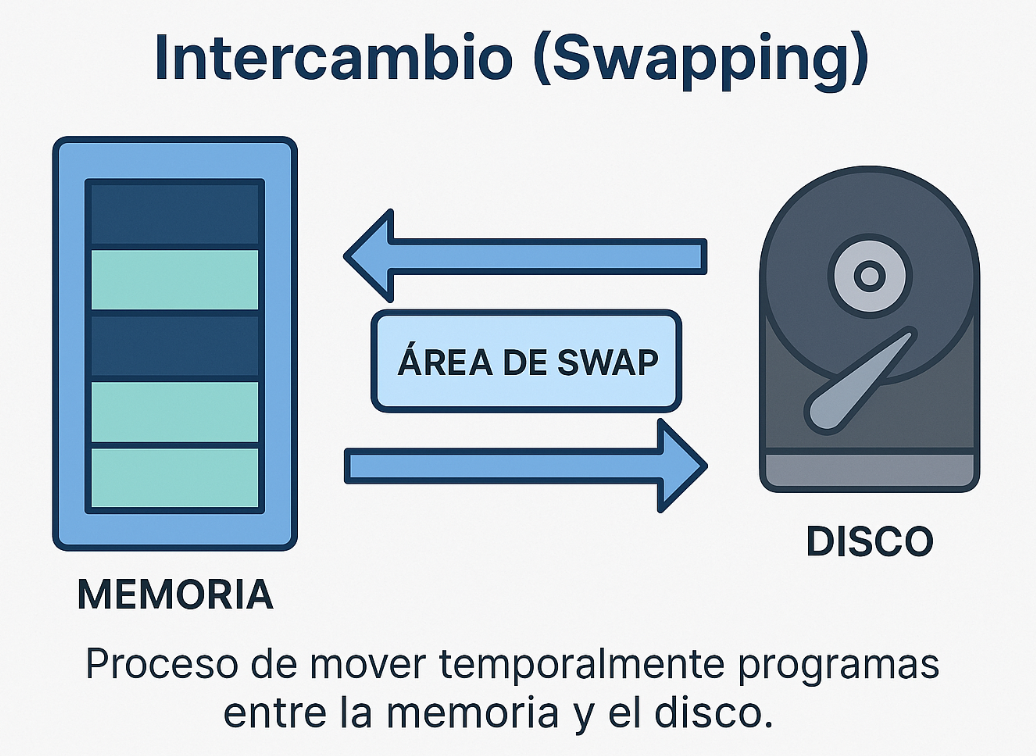
\includegraphics[width=0.7\linewidth,height=\textheight,keepaspectratio]{capitulos/img/capitulo14/14_swapping.png}
\end{center}

El principio es:

\begin{Shaded}
\begin{Highlighting}[]
\NormalTok{RAM llena}
\NormalTok{   ↓}
\NormalTok{seleccionar información/proceso que puede salir temporalmente}
\NormalTok{   ↓}
\NormalTok{mover al almacenamiento}
\NormalTok{   ↓}
\NormalTok{liberar RAM}
\NormalTok{   ↓}
\NormalTok{cuando vuelva a necesitarse}
\NormalTok{   ↓}
\NormalTok{recuperar información}
\end{Highlighting}
\end{Shaded}

\begin{tcolorbox}[enhanced jigsaw, arc=.35mm, bottomrule=.15mm, bottomtitle=1mm, breakable, colback=white, colbacktitle=quarto-callout-important-color!10!white, colframe=quarto-callout-important-color-frame, coltitle=black, left=2mm, leftrule=.75mm, opacityback=0, opacitybacktitle=0.6, rightrule=.15mm, title=\textcolor{quarto-callout-important-color}{\faExclamation}\hspace{0.5em}{Costo del intercambio}, titlerule=0mm, toprule=.15mm, toptitle=1mm]

El almacenamiento secundario es mucho más lento que la RAM. Por eso
intercambiar continuamente información puede degradar notablemente el
rendimiento.

\end{tcolorbox}

\begin{center}\rule{0.5\linewidth}{0.5pt}\end{center}

\bookmarksetup{startatroot}

\chapter{11. Swapping y paginación: no son exactamente lo
mismo}\label{swapping-y-paginaciuxf3n-no-son-exactamente-lo-mismo}

Conviene diferenciar dos ideas.

{\def\LTcaptype{none} % do not increment counter
\begin{longtable}[]{@{}
  >{\raggedright\arraybackslash}p{(\linewidth - 2\tabcolsep) * \real{0.5000}}
  >{\raggedright\arraybackslash}p{(\linewidth - 2\tabcolsep) * \real{0.5000}}@{}}
\toprule\noalign{}
\begin{minipage}[b]{\linewidth}\raggedright
Concepto
\end{minipage} & \begin{minipage}[b]{\linewidth}\raggedright
Idea principal
\end{minipage} \\
\midrule\noalign{}
\endhead
\bottomrule\noalign{}
\endlastfoot
\textbf{Swapping clásico} & Mover temporalmente grandes regiones o
procesos entre RAM y almacenamiento \\
\textbf{Paginación / memoria virtual} & Gestionar la memoria en páginas
y permitir que determinadas páginas no estén actualmente en RAM \\
\end{longtable}
}

En sistemas modernos, la gestión de memoria virtual basada en páginas
permite trabajar con una granularidad mucho más fina que el intercambio
clásico de un proceso completo.

\begin{tcolorbox}[enhanced jigsaw, arc=.35mm, bottomrule=.15mm, bottomtitle=1mm, breakable, colback=white, colbacktitle=quarto-callout-note-color!10!white, colframe=quarto-callout-note-color-frame, coltitle=black, left=2mm, leftrule=.75mm, opacityback=0, opacitybacktitle=0.6, rightrule=.15mm, title=\textcolor{quarto-callout-note-color}{\faInfo}\hspace{0.5em}{Conexión}, titlerule=0mm, toprule=.15mm, toptitle=1mm]

Esto explica por qué la paginación estudiada anteriormente es tan
importante: prepara el camino para administrar qué páginas permanecen en
RAM y cuáles pueden obtenerse desde almacenamiento cuando se necesiten.

\end{tcolorbox}

\begin{center}\rule{0.5\linewidth}{0.5pt}\end{center}

\bookmarksetup{startatroot}

\chapter{12. Administración durante la
ejecución}\label{administraciuxf3n-durante-la-ejecuciuxf3n}

Podemos representar el ciclo general de memoria así:

\begin{center}
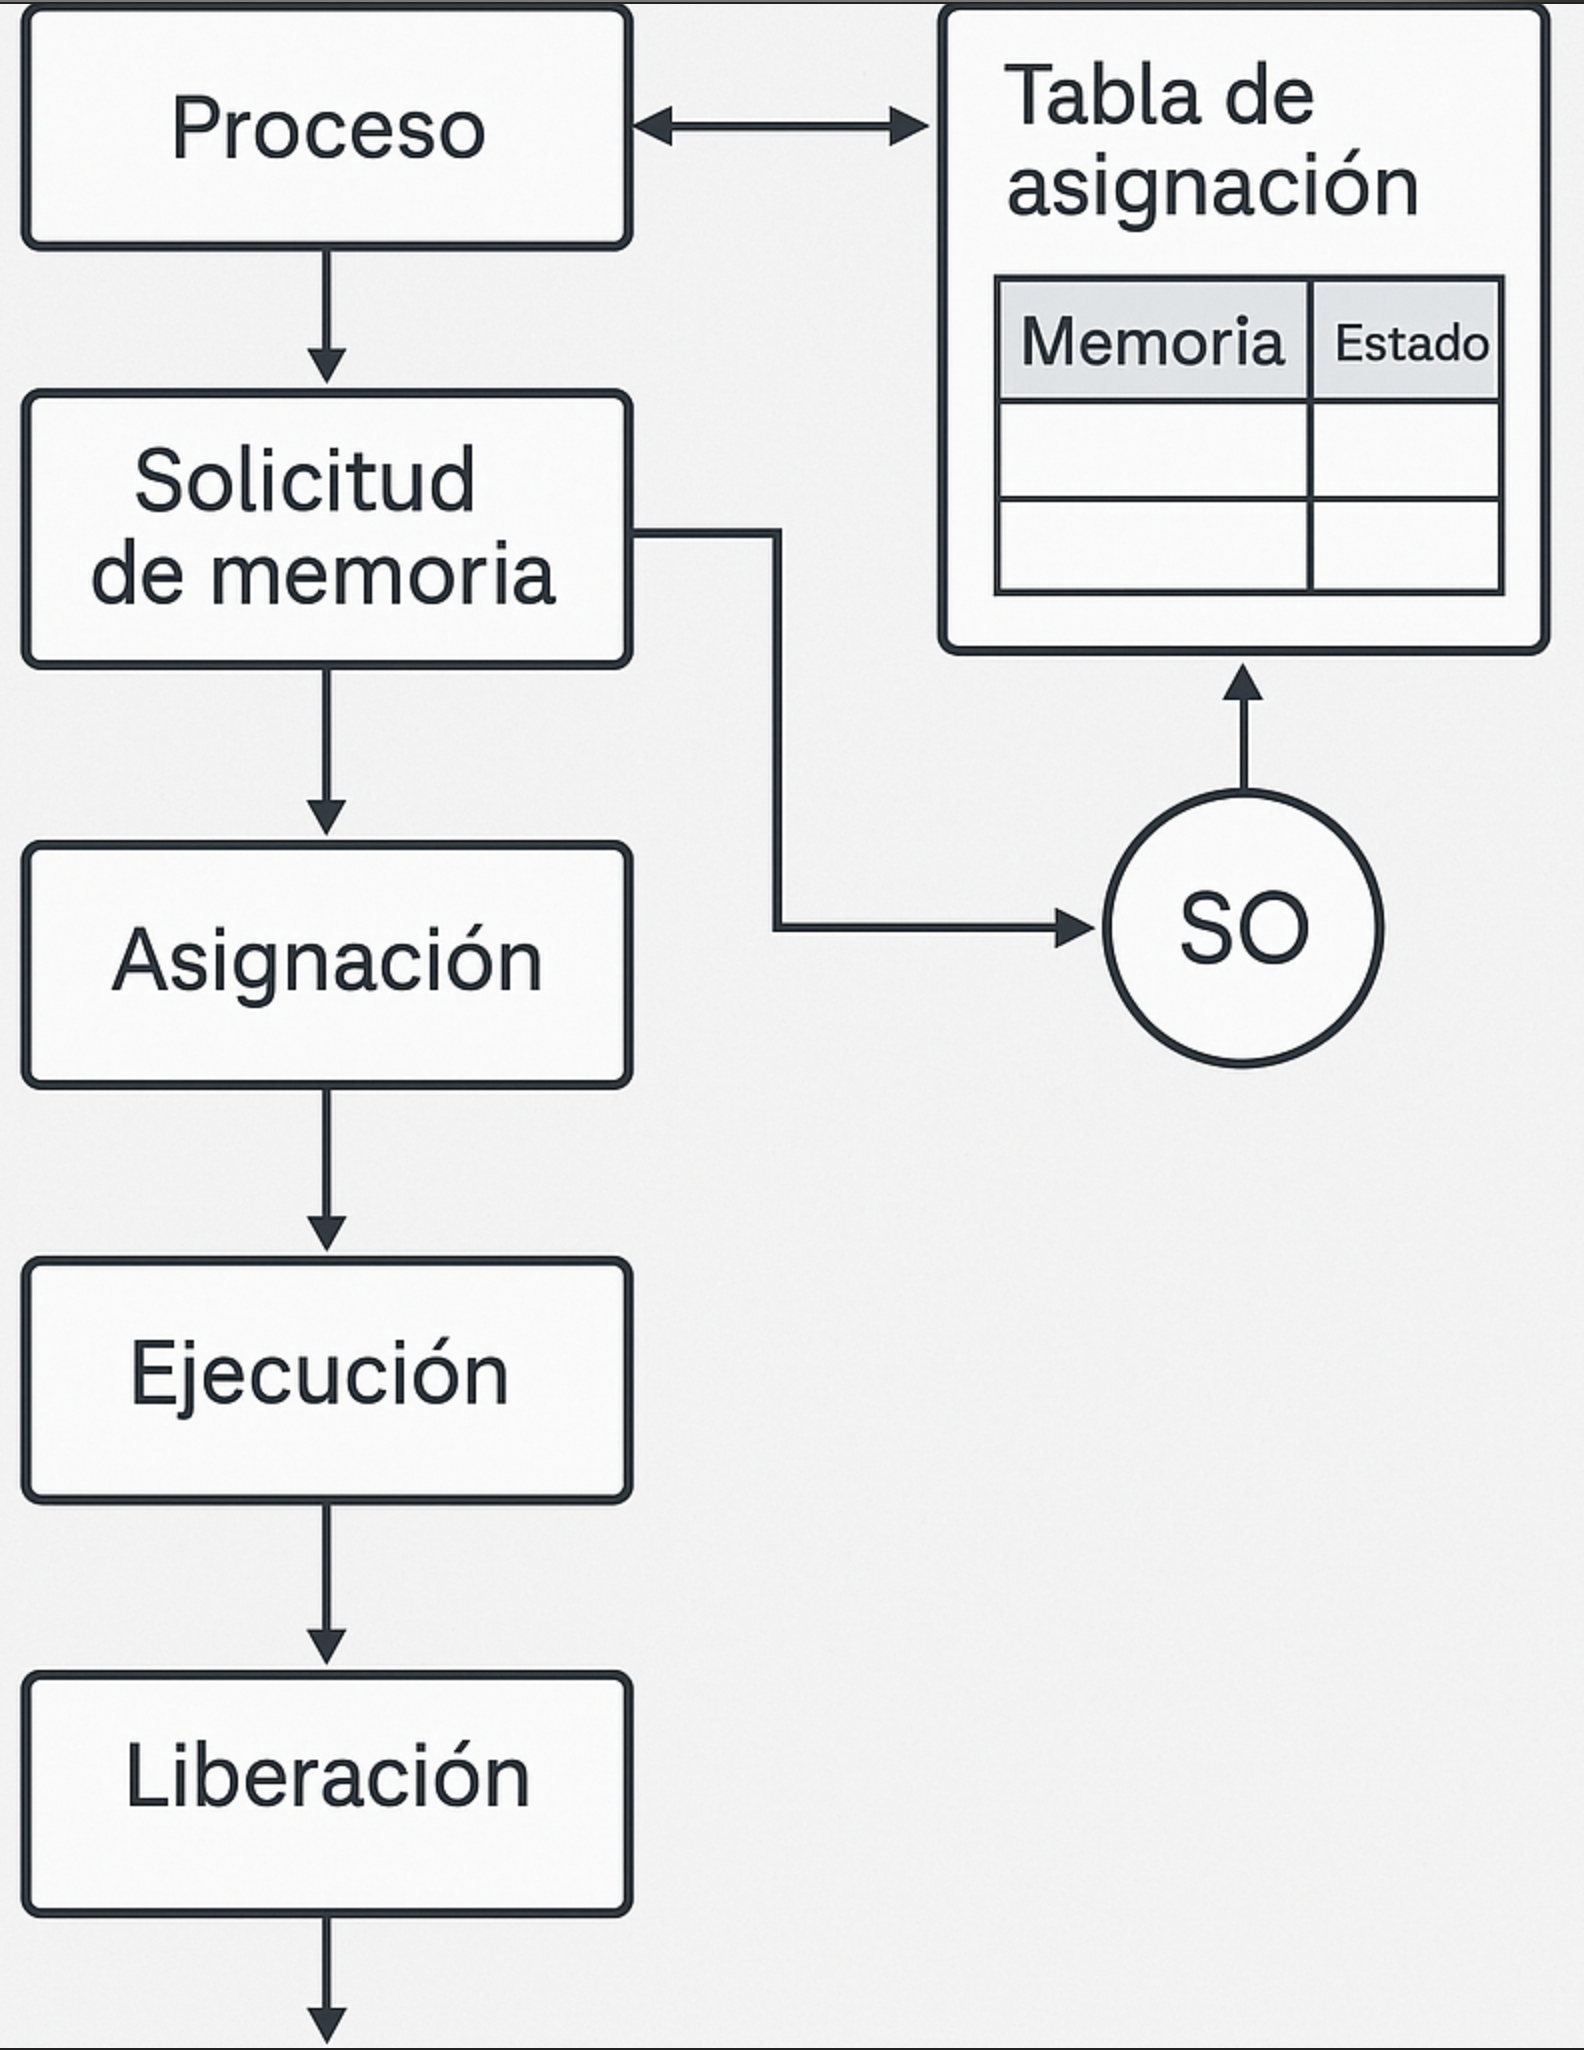
\includegraphics[width=0.67\linewidth,height=\textheight,keepaspectratio]{capitulos/img/capitulo14/14_flujo_administracion.png}
\end{center}

\begin{Shaded}
\begin{Highlighting}[]
\NormalTok{Proceso}
\NormalTok{   ↓}
\NormalTok{Solicitud de memoria}
\NormalTok{   ↓}
\NormalTok{¿Existe espacio / marco disponible?}
\NormalTok{   ↓}
\NormalTok{Asignación}
\NormalTok{   ↓}
\NormalTok{Protección y registro}
\NormalTok{   ↓}
\NormalTok{Ejecución}
\NormalTok{   ↓}
\NormalTok{Liberación}
\NormalTok{   ↓}
\NormalTok{Memoria disponible nuevamente}
\end{Highlighting}
\end{Shaded}

El Sistema Operativo debe repetir estas decisiones para muchos procesos
durante toda la ejecución del sistema.

\begin{center}\rule{0.5\linewidth}{0.5pt}\end{center}

\bookmarksetup{startatroot}

\chapter{13. Cuando necesitamos una página que no está en
RAM}\label{cuando-necesitamos-una-puxe1gina-que-no-estuxe1-en-ram}

La memoria virtual introduce una situación nueva:

\begin{quote}
El proceso intenta utilizar una página válida, pero esa página no se
encuentra actualmente cargada en RAM.
\end{quote}

Conceptualmente ocurre un \textbf{fallo de página (page fault)}.

El flujo simplificado es:

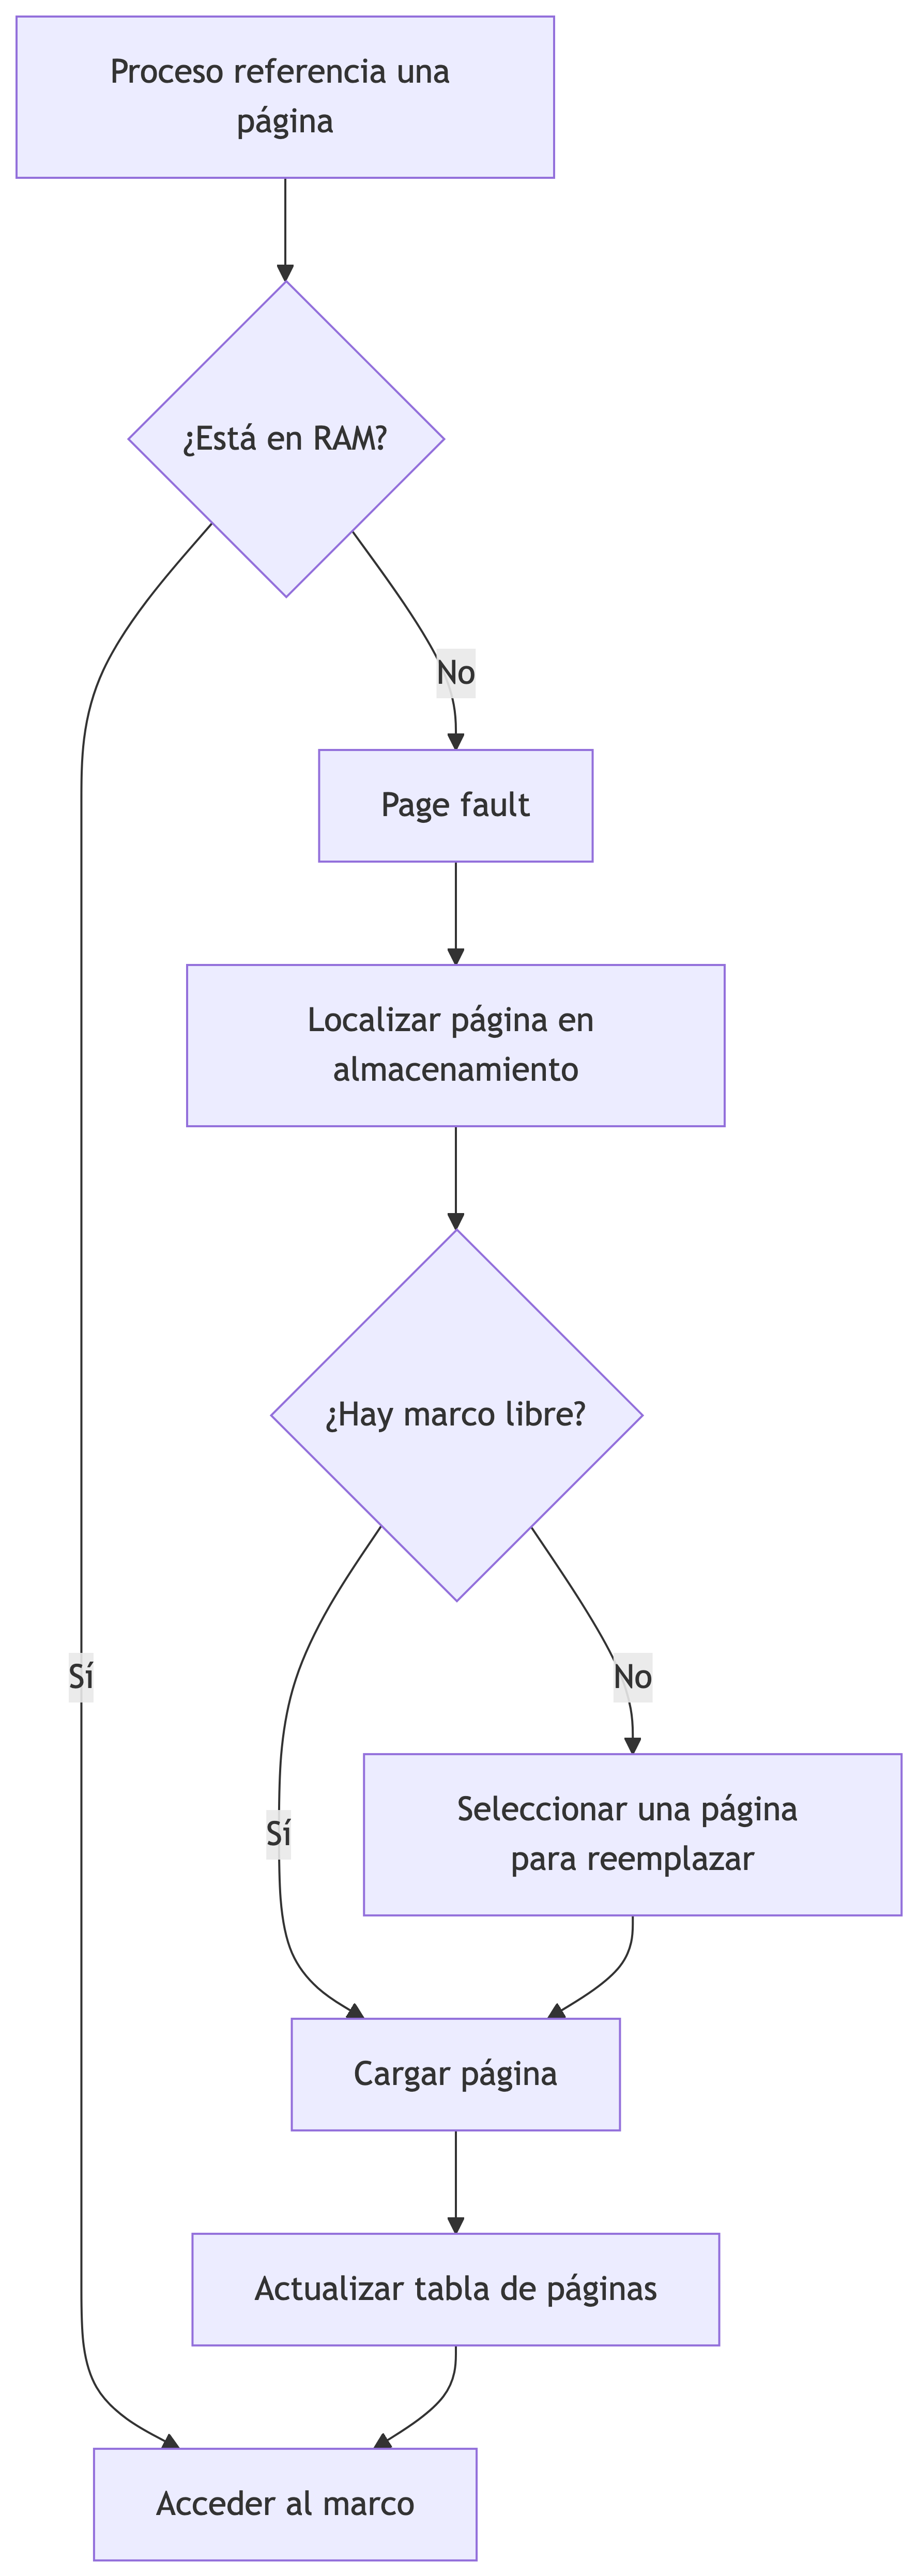
\includegraphics[width=7.4in,height=5.2in]{capitulos/14_administracion_memoria_en_ejecucion_files/figure-latex/mermaid-figure-2.png}

Ahora aparece otra pregunta:

\begin{quote}
\textbf{Si no existe un marco libre, ¿qué página deberíamos retirar?}
\end{quote}

\begin{center}\rule{0.5\linewidth}{0.5pt}\end{center}

\bookmarksetup{startatroot}

\chapter{14. Introducción a los algoritmos de
reemplazo}\label{introducciuxf3n-a-los-algoritmos-de-reemplazo}

Cuando es necesario liberar un marco, el Sistema Operativo necesita una
\textbf{política de reemplazo}.

Existen diferentes estrategias. En esta clase introduciremos una de las
más conocidas conceptualmente: \textbf{LRU (Least Recently Used)}.

LRU intenta reemplazar la página cuyo uso más reciente ocurrió hace más
tiempo.

Podemos expresarlo como:

\begin{quote}
``Si una página no se ha utilizado recientemente, puede ser una
candidata para salir de RAM''.
\end{quote}

Supongamos que el orden de uso reciente es:

\begin{Shaded}
\begin{Highlighting}[]
\NormalTok{Más antiguo                  Más reciente}
\NormalTok{Página 2 → Página 5 → Página 1 → Página 3}
\end{Highlighting}
\end{Shaded}

Si necesitamos seleccionar una candidata según LRU:

\begin{Shaded}
\begin{Highlighting}[]
\NormalTok{Página 2}
\end{Highlighting}
\end{Shaded}

\begin{tcolorbox}[enhanced jigsaw, arc=.35mm, bottomrule=.15mm, bottomtitle=1mm, breakable, colback=white, colbacktitle=quarto-callout-note-color!10!white, colframe=quarto-callout-note-color-frame, coltitle=black, left=2mm, leftrule=.75mm, opacityback=0, opacitybacktitle=0.6, rightrule=.15mm, title=\textcolor{quarto-callout-note-color}{\faInfo}\hspace{0.5em}{Importante}, titlerule=0mm, toprule=.15mm, toptitle=1mm]

LRU es una \textbf{política de reemplazo de páginas}, no un algoritmo de
asignación de particiones como First Fit, Best Fit o Worst Fit.

\end{tcolorbox}

\begin{center}\rule{0.5\linewidth}{0.5pt}\end{center}

\bookmarksetup{startatroot}

\chapter{15. Caso integrador: 1024 KB de
RAM}\label{caso-integrador-1024-kb-de-ram}

Analicemos un caso similar al material de clase, pero ajustado para que
la memoria inicial sea válida.

Tenemos:

\begin{Shaded}
\begin{Highlighting}[]
\NormalTok{RAM total = 1024 KB}

\NormalTok{P1 = 200 KB}
\NormalTok{P2 = 250 KB}
\NormalTok{P3 = 300 KB}
\end{Highlighting}
\end{Shaded}

\section{Paso 1. Memoria utilizada}\label{paso-1.-memoria-utilizada}

\begin{Shaded}
\begin{Highlighting}[]
\NormalTok{200 + 250 + 300 = 750 KB}
\end{Highlighting}
\end{Shaded}

\section{Paso 2. Memoria libre}\label{paso-2.-memoria-libre}

\begin{Shaded}
\begin{Highlighting}[]
\NormalTok{1024 {-} 750 = 274 KB}
\end{Highlighting}
\end{Shaded}

Ahora llega:

\begin{Shaded}
\begin{Highlighting}[]
\NormalTok{P4 = 300 KB}
\end{Highlighting}
\end{Shaded}

Preguntas:

\begin{enumerate}
\def\labelenumi{\arabic{enumi}.}
\tightlist
\item
  ¿Cabe P4 directamente en los 274 KB libres?
\item
  ¿Qué alternativas podría considerar el Sistema Operativo?
\item
  ¿Cambiaría el análisis si utilizamos memoria virtual y paginación?
\end{enumerate}

\begin{tcolorbox}[enhanced jigsaw, arc=.35mm, bottomrule=.15mm, bottomtitle=1mm, breakable, colback=white, colbacktitle=quarto-callout-tip-color!10!white, colframe=quarto-callout-tip-color-frame, coltitle=black, left=2mm, leftrule=.75mm, opacityback=0, opacitybacktitle=0.6, rightrule=.15mm, title=\textcolor{quarto-callout-tip-color}{\faLightbulb}\hspace{0.5em}{✅ Analicemos}, titlerule=0mm, toprule=.15mm, toptitle=1mm]

P4 necesita \textbf{300 KB}, pero solamente existen \textbf{274 KB}
disponibles en RAM.

Por tanto, no cabe completamente en la memoria libre disponible bajo un
modelo simple de asignación contigua.

Dependiendo del mecanismo utilizado, el sistema podría necesitar liberar
memoria, intercambiar información con almacenamiento o, en un esquema de
memoria virtual, administrar las páginas necesarias sin exigir que todo
el proceso se encuentre simultáneamente en RAM.

\end{tcolorbox}

\begin{tcolorbox}[enhanced jigsaw, arc=.35mm, bottomrule=.15mm, bottomtitle=1mm, breakable, colback=white, colbacktitle=quarto-callout-warning-color!10!white, colframe=quarto-callout-warning-color-frame, coltitle=black, left=2mm, leftrule=.75mm, opacityback=0, opacitybacktitle=0.6, rightrule=.15mm, title=\textcolor{quarto-callout-warning-color}{\faExclamationTriangle}\hspace{0.5em}{Ajuste didáctico respecto al PPT}, titlerule=0mm, toprule=.15mm, toptitle=1mm]

En el caso original de la presentación aparecen \texttt{P1\ =\ 200\ KB},
\texttt{P2\ =\ 350\ KB} y \texttt{P3\ =\ 500\ KB} dentro de una RAM de
\texttt{1024\ KB}. Esos tres procesos suman \textbf{1050 KB}, por lo que
ya exceden la RAM antes de que llegue P4. Para este capítulo ajustamos
los valores y conservamos la intención del ejercicio: analizar qué
ocurre cuando llega un proceso que ya no cabe en la memoria disponible.

\end{tcolorbox}

\begin{center}\rule{0.5\linewidth}{0.5pt}\end{center}

\bookmarksetup{startatroot}

\chapter{16. Simulemos un mapa de
memoria}\label{simulemos-un-mapa-de-memoria}

La presentación propone como repaso un administrador sencillo capaz de:

\begin{itemize}
\tightlist
\item
  asignar bloques;
\item
  liberar espacios;
\item
  mostrar el mapa de memoria.
\end{itemize}

\begin{center}
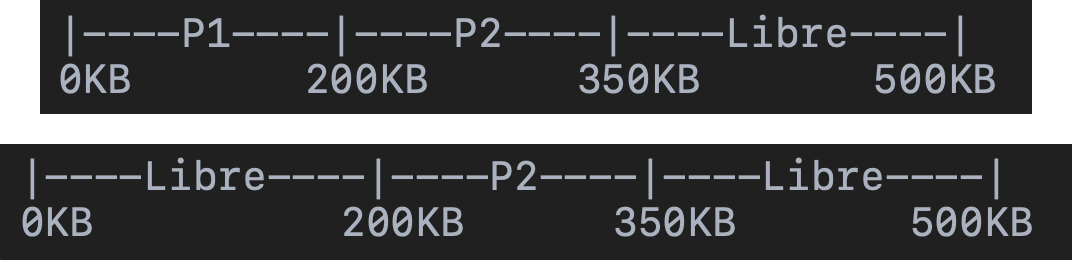
\includegraphics[width=0.72\linewidth,height=\textheight,keepaspectratio]{capitulos/img/capitulo14/14_simulacion_memoria.png}
\end{center}

Antes de programar algo así, deberíamos poder representar manualmente:

\begin{Shaded}
\begin{Highlighting}[]
\NormalTok{[ P1 ][   P2   ][ Libre ]}
\end{Highlighting}
\end{Shaded}

Luego liberar P1:

\begin{Shaded}
\begin{Highlighting}[]
\NormalTok{[Libre][   P2   ][ Libre ]}
\end{Highlighting}
\end{Shaded}

Y finalmente decidir qué hacer cuando llegue otro proceso.

\begin{tcolorbox}[enhanced jigsaw, arc=.35mm, bottomrule=.15mm, bottomtitle=1mm, breakable, colback=white, colbacktitle=quarto-callout-tip-color!10!white, colframe=quarto-callout-tip-color-frame, coltitle=black, left=2mm, leftrule=.75mm, opacityback=0, opacitybacktitle=0.6, rightrule=.15mm, title=\textcolor{quarto-callout-tip-color}{\faLightbulb}\hspace{0.5em}{Conexión con el proyecto integrador}, titlerule=0mm, toprule=.15mm, toptitle=1mm]

Este modelo es una buena base para el componente de
\textbf{Administración de Memoria} del simulador del curso: primero
comprender el mapa y las decisiones; después representarlas mediante
código.

\end{tcolorbox}

\begin{center}\rule{0.5\linewidth}{0.5pt}\end{center}

\bookmarksetup{startatroot}

\chapter{17. Sistemas reales: una precisión
importante}\label{sistemas-reales-una-precisiuxf3n-importante}

La presentación utiliza Windows y Linux para ejemplificar memoria
virtual, paginación y espacio de intercambio. La idea general es
correcta: ambos sistemas modernos utilizan \textbf{memoria virtual} y
mecanismos de paginación.

Para mantener el modelo conceptual actualizado, conviene evitar
interpretar que Linux moderno administra normalmente la memoria de
usuario mediante \textbf{segmentación en lugar de paginación}. En
arquitecturas actuales como x86-64, la paginación es el mecanismo
fundamental de traducción y protección de memoria virtual; el uso de
segmentación es mucho más limitado.

Podemos conservar esta comparación conceptual:

{\def\LTcaptype{none} % do not increment counter
\begin{longtable}[]{@{}
  >{\raggedright\arraybackslash}p{(\linewidth - 4\tabcolsep) * \real{0.3333}}
  >{\raggedright\arraybackslash}p{(\linewidth - 4\tabcolsep) * \real{0.3333}}
  >{\raggedright\arraybackslash}p{(\linewidth - 4\tabcolsep) * \real{0.3333}}@{}}
\toprule\noalign{}
\begin{minipage}[b]{\linewidth}\raggedright
Aspecto
\end{minipage} & \begin{minipage}[b]{\linewidth}\raggedright
Windows
\end{minipage} & \begin{minipage}[b]{\linewidth}\raggedright
Linux
\end{minipage} \\
\midrule\noalign{}
\endhead
\bottomrule\noalign{}
\endlastfoot
Memoria virtual & Sí & Sí \\
Paginación & Sí & Sí \\
Respaldo en almacenamiento & Archivo de paginación & Área o archivo
swap \\
Protección por proceso & Sí & Sí \\
\end{longtable}
}

\begin{center}\rule{0.5\linewidth}{0.5pt}\end{center}

\bookmarksetup{startatroot}

\chapter{18. Caso de análisis final}\label{caso-de-anuxe1lisis-final}

Tenemos una memoria representada así:

\begin{Shaded}
\begin{Highlighting}[]
\NormalTok{0 KB                                          1000 KB}
\NormalTok{|{-}{-}{-}{-}P1{-}{-}{-}{-}|{-}{-}Libre{-}{-}|{-}{-}{-}{-}{-}{-}P2{-}{-}{-}{-}{-}{-}|{-}{-}{-}Libre{-}{-}{-}|}
\NormalTok{    200       150          400          250}
\end{Highlighting}
\end{Shaded}

Llega:

\begin{Shaded}
\begin{Highlighting}[]
\NormalTok{P3 = 300 KB}
\end{Highlighting}
\end{Shaded}

Analiza:

\begin{enumerate}
\def\labelenumi{\arabic{enumi}.}
\tightlist
\item
  ¿Cuánta memoria libre existe en total?
\item
  ¿Existe un bloque contiguo de 300 KB?
\item
  ¿Qué problema aparece?
\item
  ¿Serviría la compactación?
\item
  ¿Qué ventaja ofrecería un esquema paginado?
\item
  Si una página necesaria no estuviera en RAM, ¿qué evento podría
  producirse?
\item
  Si no hubiera marcos libres, ¿qué tipo de algoritmo necesitaríamos?
\end{enumerate}

\begin{tcolorbox}[enhanced jigsaw, arc=.35mm, bottomrule=.15mm, bottomtitle=1mm, breakable, colback=white, colbacktitle=quarto-callout-tip-color!10!white, colframe=quarto-callout-tip-color-frame, coltitle=black, left=2mm, leftrule=.75mm, opacityback=0, opacitybacktitle=0.6, rightrule=.15mm, title=\textcolor{quarto-callout-tip-color}{\faLightbulb}\hspace{0.5em}{✅ Solución propuesta}, titlerule=0mm, toprule=.15mm, toptitle=1mm]

Existe:

\begin{Shaded}
\begin{Highlighting}[]
\NormalTok{150 + 250 = 400 KB libres}
\end{Highlighting}
\end{Shaded}

pero el bloque libre más grande es de \texttt{250\ KB}.

Por tanto, P3 no cabe como bloque contiguo de \texttt{300\ KB}, aunque
existe suficiente memoria libre \textbf{en total}. Esto representa
\textbf{fragmentación externa}.

La compactación podría reunir los espacios libres, aunque implica costo
de movimiento. Un esquema paginado permitiría colocar las páginas en
marcos no contiguos. Si una página válida no estuviera cargada, se
produciría un \textbf{page fault}. Si no hubiera marcos libres, sería
necesaria una política de \textbf{reemplazo de páginas}.

\end{tcolorbox}

\begin{center}\rule{0.5\linewidth}{0.5pt}\end{center}

\bookmarksetup{startatroot}

\chapter{19. Autoevaluación}\label{autoevaluaciuxf3n-9}

\begin{enumerate}
\def\labelenumi{\arabic{enumi}.}
\tightlist
\item
  ¿Cuáles son las cinco funciones principales del administrador de
  memoria?
\item
  ¿Por qué la memoria se organiza jerárquicamente?
\item
  ¿Qué diferencia existe entre RAM y caché?
\item
  ¿Qué diferencia existe entre dirección lógica y física?
\item
  ¿Qué función cumple conceptualmente la MMU?
\item
  ¿Qué representan los registros base y límite?
\item
  ¿Por qué la protección de memoria es necesaria?
\item
  ¿Qué información puede mostrar un mapa de memoria?
\item
  ¿Qué significa liberar memoria?
\item
  ¿Qué problema intenta resolver la compactación?
\item
  ¿Qué es swapping?
\item
  ¿Por qué demasiado intercambio reduce el rendimiento?
\item
  ¿Qué es un page fault?
\item
  ¿Cuándo necesitamos un algoritmo de reemplazo de páginas?
\item
  ¿Cuál es la idea fundamental de LRU?
\item
  ¿Qué relación existe entre paginación y memoria virtual?
\end{enumerate}

\begin{center}\rule{0.5\linewidth}{0.5pt}\end{center}

\bookmarksetup{startatroot}

\chapter{20. Para recordar}\label{para-recordar-5}

\begin{Shaded}
\begin{Highlighting}[]
\NormalTok{CPU NECESITA DATOS}
\NormalTok{      ↓}
\NormalTok{JERARQUÍA DE MEMORIA}
\NormalTok{      ↓}
\NormalTok{CACHÉ → RAM → ALMACENAMIENTO}
\NormalTok{      ↓}
\NormalTok{PROCESO SOLICITA MEMORIA}
\NormalTok{      ↓}
\NormalTok{ASIGNAR + REGISTRAR + PROTEGER}
\NormalTok{      ↓}
\NormalTok{DIRECCIÓN LÓGICA → TRADUCCIÓN → FÍSICA}
\NormalTok{      ↓}
\NormalTok{EJECUCIÓN}
\NormalTok{      ↓}
\NormalTok{LIBERAR MEMORIA}
\NormalTok{      ↓}
\NormalTok{SI FALTA RAM}
\NormalTok{      ↓}
\NormalTok{MEMORIA VIRTUAL / INTERCAMBIO}
\NormalTok{      ↓}
\NormalTok{PAGE FAULT}
\NormalTok{      ↓}
\NormalTok{¿HAY MARCO LIBRE?}
\NormalTok{      ↓ NO}
\NormalTok{REEMPLAZO DE PÁGINAS (ej. LRU)}
\end{Highlighting}
\end{Shaded}

Administrar memoria significa mucho más que encontrar un espacio libre.
El Sistema Operativo debe \textbf{saber dónde están los datos,
protegerlos, traducir direcciones, mover información entre niveles y
recuperar el espacio cuando deja de utilizarse}.

\begin{center}\rule{0.5\linewidth}{0.5pt}\end{center}

\bookmarksetup{startatroot}

\chapter{Conexión con la siguiente
clase}\label{conexiuxf3n-con-la-siguiente-clase-3}

Ya conocemos las estructuras de organización de memoria y el ciclo
operativo de asignación, protección, liberación e intercambio.

El siguiente paso natural es profundizar en \textbf{memoria virtual y
algoritmos de reemplazo de páginas}, comparando cómo diferentes
políticas deciden qué información debe permanecer en RAM cuando la
memoria física es insuficiente.

\begin{center}\rule{0.5\linewidth}{0.5pt}\end{center}

\bookmarksetup{startatroot}

\chapter{Referencias}\label{referencias-2}

Material base de clase:

\begin{itemize}
\tightlist
\item
  Presentación \textbf{Administración de Memoria}, Sistemas Operativos
  I.
\item
  Capítulo anterior del libro: \textbf{Manejo de memoria: particiones y
  paginación}.
\end{itemize}

\begin{tcolorbox}[enhanced jigsaw, arc=.35mm, bottomrule=.15mm, bottomtitle=1mm, breakable, colback=white, colbacktitle=quarto-callout-note-color!10!white, colframe=quarto-callout-note-color-frame, coltitle=black, left=2mm, leftrule=.75mm, opacityback=0, opacitybacktitle=0.6, rightrule=.15mm, title=\textcolor{quarto-callout-note-color}{\faInfo}\hspace{0.5em}{Criterio editorial}, titlerule=0mm, toprule=.15mm, toptitle=1mm]

Este capítulo reorganiza la presentación para evitar repetir en
profundidad particiones y paginación, ya desarrolladas en el capítulo
anterior. Se conservaron como eje las ideas de \textbf{jerarquía,
protección, mapas de memoria, swapping, administración en ejecución y
LRU}, y se corrigieron explícitamente dos simplificaciones del material
original para mantener consistencia técnica.

\end{tcolorbox}

\bookmarksetup{startatroot}

\chapter{Capítulo 15. Métodos de ajuste de
memoria}\label{capuxedtulo-15.-muxe9todos-de-ajuste-de-memoria}

¿Dónde debe colocar el Sistema Operativo un nuevo proceso?

\hfill\break

\bookmarksetup{startatroot}

\chapter{Capítulo 15. Métodos de ajuste de
memoria}\label{capuxedtulo-15.-muxe9todos-de-ajuste-de-memoria-1}

\section{De conocer el mapa de memoria a tomar una
decisión}\label{de-conocer-el-mapa-de-memoria-a-tomar-una-decisiuxf3n}

En el capítulo anterior estudiamos la \textbf{administración de memoria
durante la ejecución}. Vimos que el Sistema Operativo debe saber qué
regiones están ocupadas, cuáles están libres, proteger los espacios de
cada proceso y recuperar memoria cuando deja de utilizarse.

Ahora aparece una pregunta muy concreta:

\begin{quote}
\textbf{Si existen varios espacios libres, ¿en cuál debemos colocar un
nuevo proceso?}
\end{quote}

No siempre existe una única respuesta.

La decisión dependerá de la estrategia de asignación utilizada.

\begin{tcolorbox}[enhanced jigsaw, arc=.35mm, bottomrule=.15mm, bottomtitle=1mm, breakable, colback=white, colbacktitle=quarto-callout-tip-color!10!white, colframe=quarto-callout-tip-color-frame, coltitle=black, left=2mm, leftrule=.75mm, opacityback=0, opacitybacktitle=0.6, rightrule=.15mm, title=\textcolor{quarto-callout-tip-color}{\faLightbulb}\hspace{0.5em}{Idea central}, titlerule=0mm, toprule=.15mm, toptitle=1mm]

Los métodos \textbf{First Fit, Best Fit y Worst Fit} responden a la
misma pregunta, pero utilizan criterios diferentes para seleccionar un
hueco libre.

\end{tcolorbox}

\begin{center}\rule{0.5\linewidth}{0.5pt}\end{center}

\bookmarksetup{startatroot}

\chapter{Objetivos de aprendizaje}\label{objetivos-de-aprendizaje-11}

Al finalizar este capítulo, el estudiante será capaz de:

\begin{itemize}
\tightlist
\item
  Explicar qué problema resuelven los métodos de ajuste de memoria.
\item
  Aplicar manualmente \textbf{First Fit}, \textbf{Best Fit} y
  \textbf{Worst Fit}.
\item
  Diferenciar el criterio de selección utilizado por cada estrategia.
\item
  Calcular el espacio restante después de una asignación.
\item
  Relacionar las decisiones de ajuste con la \textbf{fragmentación
  externa}.
\item
  Explicar qué hace la compactación y por qué tiene un costo.
\item
  Comparar las estrategias utilizando una misma secuencia de procesos.
\item
  Distinguir estos algoritmos didácticos de los mecanismos de memoria
  usados por sistemas modernos.
\end{itemize}

\begin{center}\rule{0.5\linewidth}{0.5pt}\end{center}

\bookmarksetup{startatroot}

\chapter{1. Partamos de una situación
real}\label{partamos-de-una-situaciuxf3n-real}

Imaginemos que el Sistema Operativo observa este mapa:

\begin{Shaded}
\begin{Highlighting}[]
\NormalTok{Memoria}
\NormalTok{┌──────────┬──────────┬──────────┐}
\NormalTok{│ Libre    │ Libre    │ Libre    │}
\NormalTok{│ 100 KB   │ 200 KB   │ 300 KB   │}
\NormalTok{└──────────┴──────────┴──────────┘}
\end{Highlighting}
\end{Shaded}

Llega un proceso:

\begin{Shaded}
\begin{Highlighting}[]
\NormalTok{P1 = 120 KB}
\end{Highlighting}
\end{Shaded}

Preguntemos primero:

\begin{quote}
\textbf{¿En cuáles bloques cabe P1?}
\end{quote}

\begin{itemize}
\tightlist
\item
  \texttt{100\ KB} → no cabe.
\item
  \texttt{200\ KB} → sí cabe.
\item
  \texttt{300\ KB} → sí cabe.
\end{itemize}

Tenemos \textbf{dos candidatos válidos}.

El problema ya no es simplemente saber si existe memoria.

El Sistema Operativo debe decidir:

\begin{quote}
\textbf{¿Cuál de los bloques disponibles utilizar?}
\end{quote}

\begin{center}\rule{0.5\linewidth}{0.5pt}\end{center}

\bookmarksetup{startatroot}

\chapter{2. ¿Qué es un método de
ajuste?}\label{quuxe9-es-un-muxe9todo-de-ajuste}

Un método de ajuste es una estrategia para seleccionar un \textbf{hueco
o bloque libre} donde pueda colocarse una solicitud de memoria bajo un
modelo de asignación contigua.

Podemos representar el problema como:

\includegraphics[width=7.2in,height=4.3in]{capitulos/15_metodos_ajuste_memoria_con_solucion_files/figure-latex/mermaid-figure-1.png}

Una vez identificados los candidatos, necesitamos una \textbf{regla de
decisión}.

Ahí aparecen:

\begin{Shaded}
\begin{Highlighting}[]
\NormalTok{First Fit  → el primero que sirva}
\NormalTok{Best Fit   → el más pequeño que sirva}
\NormalTok{Worst Fit  → el más grande que sirva}
\end{Highlighting}
\end{Shaded}

\begin{tcolorbox}[enhanced jigsaw, arc=.35mm, bottomrule=.15mm, bottomtitle=1mm, breakable, colback=white, colbacktitle=quarto-callout-important-color!10!white, colframe=quarto-callout-important-color-frame, coltitle=black, left=2mm, leftrule=.75mm, opacityback=0, opacitybacktitle=0.6, rightrule=.15mm, title=\textcolor{quarto-callout-important-color}{\faExclamation}\hspace{0.5em}{No memoricemos todavía}, titlerule=0mm, toprule=.15mm, toptitle=1mm]

Antes de aprender los nombres, comprendamos la pregunta que responde
cada algoritmo.

\end{tcolorbox}

\begin{center}\rule{0.5\linewidth}{0.5pt}\end{center}

\bookmarksetup{startatroot}

\chapter{3. First Fit --- Primer ajuste}\label{first-fit-primer-ajuste}

\textbf{First Fit} recorre los huecos desde el inicio y selecciona el
\textbf{primer bloque suficientemente grande}.

Tenemos:

\begin{Shaded}
\begin{Highlighting}[]
\NormalTok{Huecos: 100 KB, 200 KB, 300 KB}
\NormalTok{Proceso: 120 KB}
\end{Highlighting}
\end{Shaded}

Recorrido:

\begin{Shaded}
\begin{Highlighting}[]
\NormalTok{100 KB → ¿120 cabe? NO}
\NormalTok{200 KB → ¿120 cabe? SÍ  ← detener búsqueda}
\NormalTok{300 KB → ya no necesitamos revisarlo}
\end{Highlighting}
\end{Shaded}

Por tanto:

\begin{Shaded}
\begin{Highlighting}[]
\NormalTok{First Fit selecciona 200 KB.}
\end{Highlighting}
\end{Shaded}

Después de colocar el proceso:

\begin{Shaded}
\begin{Highlighting}[]
\NormalTok{200 KB {-} 120 KB = 80 KB}
\end{Highlighting}
\end{Shaded}

El mapa conceptual queda:

\begin{Shaded}
\begin{Highlighting}[]
\NormalTok{┌────────┬──────────┬────────┬──────────┐}
\NormalTok{│ Libre  │ P1       │ Libre  │ Libre    │}
\NormalTok{│100 KB  │120 KB    │ 80 KB  │300 KB   │}
\NormalTok{└────────┴──────────┴────────┴──────────┘}
\end{Highlighting}
\end{Shaded}

\section{¿Por qué puede ser
rápido?}\label{por-quuxe9-puede-ser-ruxe1pido}

Porque puede detener la búsqueda tan pronto encuentra un espacio válido.

\begin{Shaded}
\begin{Highlighting}[]
\NormalTok{Inicio}
\NormalTok{  ↓}
\NormalTok{¿cabe?}
\NormalTok{  ↓ No}
\NormalTok{siguiente}
\NormalTok{  ↓}
\NormalTok{¿cabe?}
\NormalTok{  ↓ Sí}
\NormalTok{ASIGNAR Y TERMINAR}
\end{Highlighting}
\end{Shaded}

\subsection{Ventajas}\label{ventajas-11}

\begin{itemize}
\tightlist
\item
  criterio sencillo;
\item
  normalmente requiere poca búsqueda;
\item
  fácil de comprender e implementar.
\end{itemize}

\subsection{Limitaciones}\label{limitaciones-2}

\begin{itemize}
\tightlist
\item
  la elección depende del orden de los huecos;
\item
  puede ir dejando huecos pequeños;
\item
  no intenta encontrar la opción que deje el menor sobrante.
\end{itemize}

\begin{center}\rule{0.5\linewidth}{0.5pt}\end{center}

\bookmarksetup{startatroot}

\chapter{4. Best Fit --- Mejor ajuste}\label{best-fit-mejor-ajuste}

\textbf{Best Fit} busca el \textbf{hueco más pequeño que sea
suficientemente grande}.

La pregunta cambia:

\begin{quote}
Entre todos los bloques donde cabe el proceso, ¿cuál se aproxima más a
su tamaño?
\end{quote}

Con:

\begin{Shaded}
\begin{Highlighting}[]
\NormalTok{Huecos: 100 KB, 200 KB, 300 KB}
\NormalTok{Proceso: 120 KB}
\end{Highlighting}
\end{Shaded}

tenemos:

\begin{Shaded}
\begin{Highlighting}[]
\NormalTok{100 KB → no sirve}
\NormalTok{200 KB → sirve → sobran 80 KB}
\NormalTok{300 KB → sirve → sobran 180 KB}
\end{Highlighting}
\end{Shaded}

El menor sobrante es:

\begin{Shaded}
\begin{Highlighting}[]
\NormalTok{80 KB}
\end{Highlighting}
\end{Shaded}

Por tanto:

\begin{Shaded}
\begin{Highlighting}[]
\NormalTok{Best Fit selecciona 200 KB.}
\end{Highlighting}
\end{Shaded}

\begin{tcolorbox}[enhanced jigsaw, arc=.35mm, bottomrule=.15mm, bottomtitle=1mm, breakable, colback=white, colbacktitle=quarto-callout-note-color!10!white, colframe=quarto-callout-note-color-frame, coltitle=black, left=2mm, leftrule=.75mm, opacityback=0, opacitybacktitle=0.6, rightrule=.15mm, title=\textcolor{quarto-callout-note-color}{\faInfo}\hspace{0.5em}{¡Aquí First Fit y Best Fit dieron el mismo resultado!}, titlerule=0mm, toprule=.15mm, toptitle=1mm]

Eso puede ocurrir. Que dos algoritmos seleccionen el mismo bloque en un
caso particular \textbf{no significa que sean iguales}. Lo importante es
el criterio utilizado para tomar la decisión.

\end{tcolorbox}

\subsection{Ventaja conceptual}\label{ventaja-conceptual}

Busca reducir el sobrante de \textbf{esa asignación}.

\subsection{Limitaciones}\label{limitaciones-3}

\begin{itemize}
\tightlist
\item
  normalmente debe examinar más candidatos para saber cuál es el mejor;
\item
  puede producir huecos residuales muy pequeños y poco útiles.
\end{itemize}

\begin{center}\rule{0.5\linewidth}{0.5pt}\end{center}

\bookmarksetup{startatroot}

\chapter{5. Necesitamos un ejemplo mejor para
diferenciarlos}\label{necesitamos-un-ejemplo-mejor-para-diferenciarlos}

Cambiemos el mapa:

\begin{Shaded}
\begin{Highlighting}[]
\NormalTok{Huecos libres:}
\NormalTok{┌────────┬────────┬────────┬────────┐}
\NormalTok{│ 300 KB │ 180 KB │ 250 KB │ 500 KB │}
\NormalTok{└────────┴────────┴────────┴────────┘}

\NormalTok{Proceso nuevo:}
\NormalTok{P1 = 170 KB}
\end{Highlighting}
\end{Shaded}

\section{First Fit}\label{first-fit-1}

Empieza desde el inicio:

\begin{Shaded}
\begin{Highlighting}[]
\NormalTok{300 KB → cabe}
\end{Highlighting}
\end{Shaded}

Se detiene.

\begin{Shaded}
\begin{Highlighting}[]
\NormalTok{First Fit → 300 KB}
\NormalTok{Sobrante  → 130 KB}
\end{Highlighting}
\end{Shaded}

\section{Best Fit}\label{best-fit-1}

Busca el hueco válido más pequeño:

\begin{Shaded}
\begin{Highlighting}[]
\NormalTok{300 KB → sobra 130}
\NormalTok{180 KB → sobra 10   ← mejor candidato}
\NormalTok{250 KB → sobra 80}
\NormalTok{500 KB → sobra 330}
\end{Highlighting}
\end{Shaded}

Por tanto:

\begin{Shaded}
\begin{Highlighting}[]
\NormalTok{Best Fit → 180 KB}
\NormalTok{Sobrante → 10 KB}
\end{Highlighting}
\end{Shaded}

Ahora sí observamos claramente que los algoritmos toman decisiones
diferentes.

\begin{center}\rule{0.5\linewidth}{0.5pt}\end{center}

\bookmarksetup{startatroot}

\chapter{6. Worst Fit --- Peor ajuste}\label{worst-fit-peor-ajuste}

El nombre puede parecer extraño.

\textbf{Worst Fit} selecciona el \textbf{hueco libre más grande} donde
el proceso pueda colocarse.

Con:

\begin{Shaded}
\begin{Highlighting}[]
\NormalTok{Huecos: 300, 180, 250, 500 KB}
\NormalTok{Proceso: 170 KB}
\end{Highlighting}
\end{Shaded}

seleccionará:

\begin{Shaded}
\begin{Highlighting}[]
\NormalTok{500 KB}
\end{Highlighting}
\end{Shaded}

y quedará:

\begin{Shaded}
\begin{Highlighting}[]
\NormalTok{500 {-} 170 = 330 KB}
\end{Highlighting}
\end{Shaded}

La idea es evitar consumir un hueco pequeño y dejar, después de la
asignación, un sobrante relativamente grande que potencialmente pueda
ser útil.

\begin{Shaded}
\begin{Highlighting}[]
\NormalTok{Worst Fit → 500 KB}
\NormalTok{Sobrante  → 330 KB}
\end{Highlighting}
\end{Shaded}

\subsection{Ventaja conceptual}\label{ventaja-conceptual-1}

\begin{itemize}
\tightlist
\item
  puede conservar huecos residuales grandes.
\end{itemize}

\subsection{Limitaciones}\label{limitaciones-4}

\begin{itemize}
\tightlist
\item
  necesita identificar un hueco máximo adecuado;
\item
  puede consumir rápidamente los bloques más grandes disponibles;
\item
  no garantiza una menor fragmentación a lo largo de una carga completa.
\end{itemize}

\begin{tcolorbox}[enhanced jigsaw, arc=.35mm, bottomrule=.15mm, bottomtitle=1mm, breakable, colback=white, colbacktitle=quarto-callout-warning-color!10!white, colframe=quarto-callout-warning-color-frame, coltitle=black, left=2mm, leftrule=.75mm, opacityback=0, opacitybacktitle=0.6, rightrule=.15mm, title=\textcolor{quarto-callout-warning-color}{\faExclamationTriangle}\hspace{0.5em}{Evitemos una conclusión apresurada}, titlerule=0mm, toprule=.15mm, toptitle=1mm]

No debemos afirmar que Worst Fit ``elimina'' o necesariamente ``reduce''
la fragmentación externa. El resultado depende de la secuencia de
solicitudes y liberaciones.

\end{tcolorbox}

\begin{center}\rule{0.5\linewidth}{0.5pt}\end{center}

\bookmarksetup{startatroot}

\chapter{7. Los tres frente al mismo
problema}\label{los-tres-frente-al-mismo-problema}

Utilicemos:

\begin{Shaded}
\begin{Highlighting}[]
\NormalTok{Huecos: 300, 180, 250, 500 KB}
\NormalTok{Proceso: 170 KB}
\end{Highlighting}
\end{Shaded}

{\def\LTcaptype{none} % do not increment counter
\begin{longtable}[]{@{}lrrl@{}}
\toprule\noalign{}
Método & Bloque elegido & Sobrante inmediato & Criterio \\
\midrule\noalign{}
\endhead
\bottomrule\noalign{}
\endlastfoot
First Fit & 300 KB & 130 KB & Primer bloque suficiente \\
Best Fit & 180 KB & 10 KB & Menor bloque suficiente \\
Worst Fit & 500 KB & 330 KB & Mayor bloque suficiente \\
\end{longtable}
}

Esta tabla resume \textbf{una asignación}.

No es suficiente para declarar un ganador universal.

\begin{quote}
Para comparar estrategias de verdad necesitamos observar qué ocurre con
\textbf{varios procesos consecutivos}.
\end{quote}

\begin{center}\rule{0.5\linewidth}{0.5pt}\end{center}

\bookmarksetup{startatroot}

\chapter{8. Simulación: ahora llegan varios
procesos}\label{simulaciuxf3n-ahora-llegan-varios-procesos}

Estado inicial:

\begin{Shaded}
\begin{Highlighting}[]
\NormalTok{Huecos libres = [100, 500, 200, 300, 600] KB}
\end{Highlighting}
\end{Shaded}

Llegan, en este orden:

\begin{Shaded}
\begin{Highlighting}[]
\NormalTok{P1 = 212 KB}
\NormalTok{P2 = 417 KB}
\NormalTok{P3 = 112 KB}
\NormalTok{P4 = 426 KB}
\end{Highlighting}
\end{Shaded}

No cambiemos el orden.

El objetivo es ejecutar mentalmente cada algoritmo y observar cómo
cambia el mapa.

\begin{tcolorbox}[enhanced jigsaw, arc=.35mm, bottomrule=.15mm, bottomtitle=1mm, breakable, colback=white, colbacktitle=quarto-callout-tip-color!10!white, colframe=quarto-callout-tip-color-frame, coltitle=black, left=2mm, leftrule=.75mm, opacityback=0, opacitybacktitle=0.6, rightrule=.15mm, title=\textcolor{quarto-callout-tip-color}{\faLightbulb}\hspace{0.5em}{Método de trabajo}, titlerule=0mm, toprule=.15mm, toptitle=1mm]

En cada paso:

\begin{enumerate}
\def\labelenumi{\arabic{enumi}.}
\tightlist
\item
  observe los huecos actuales;
\item
  aplique \textbf{solamente} el criterio del algoritmo;
\item
  seleccione el hueco;
\item
  reste el tamaño del proceso;
\item
  actualice la lista de huecos;
\item
  continúe con el siguiente proceso.
\end{enumerate}

\end{tcolorbox}

\begin{center}\rule{0.5\linewidth}{0.5pt}\end{center}

\bookmarksetup{startatroot}

\chapter{9. Simulación con First Fit}\label{simulaciuxf3n-con-first-fit}

Estado inicial:

\begin{Shaded}
\begin{Highlighting}[]
\NormalTok{[100, 500, 200, 300, 600]}
\end{Highlighting}
\end{Shaded}

\section{P1 = 212 KB}\label{p1-212-kb}

\begin{Shaded}
\begin{Highlighting}[]
\NormalTok{100 → no cabe}
\NormalTok{500 → cabe}
\end{Highlighting}
\end{Shaded}

Asignamos allí:

\begin{Shaded}
\begin{Highlighting}[]
\NormalTok{500 {-} 212 = 288}
\end{Highlighting}
\end{Shaded}

Nuevo estado:

\begin{Shaded}
\begin{Highlighting}[]
\NormalTok{[100, 288, 200, 300, 600]}
\end{Highlighting}
\end{Shaded}

\section{P2 = 417 KB}\label{p2-417-kb}

\begin{Shaded}
\begin{Highlighting}[]
\NormalTok{100 → no}
\NormalTok{288 → no}
\NormalTok{200 → no}
\NormalTok{300 → no}
\NormalTok{600 → sí}
\end{Highlighting}
\end{Shaded}

\begin{Shaded}
\begin{Highlighting}[]
\NormalTok{600 {-} 417 = 183}
\end{Highlighting}
\end{Shaded}

Nuevo estado:

\begin{Shaded}
\begin{Highlighting}[]
\NormalTok{[100, 288, 200, 300, 183]}
\end{Highlighting}
\end{Shaded}

\section{P3 = 112 KB}\label{p3-112-kb}

\begin{Shaded}
\begin{Highlighting}[]
\NormalTok{100 → no}
\NormalTok{288 → sí}
\end{Highlighting}
\end{Shaded}

\begin{Shaded}
\begin{Highlighting}[]
\NormalTok{288 {-} 112 = 176}
\end{Highlighting}
\end{Shaded}

Nuevo estado:

\begin{Shaded}
\begin{Highlighting}[]
\NormalTok{[100, 176, 200, 300, 183]}
\end{Highlighting}
\end{Shaded}

\section{P4 = 426 KB}\label{p4-426-kb}

Revisamos:

\begin{Shaded}
\begin{Highlighting}[]
\NormalTok{100, 176, 200, 300, 183}
\end{Highlighting}
\end{Shaded}

Ningún hueco alcanza \texttt{426\ KB}.

\begin{Shaded}
\begin{Highlighting}[]
\NormalTok{P4 → NO PUEDE ASIGNARSE}
\end{Highlighting}
\end{Shaded}

\begin{center}\rule{0.5\linewidth}{0.5pt}\end{center}

\bookmarksetup{startatroot}

\chapter{10. ¿Falta memoria o está
fragmentada?}\label{falta-memoria-o-estuxe1-fragmentada}

Después de First Fit tenemos:

\begin{Shaded}
\begin{Highlighting}[]
\NormalTok{100 + 176 + 200 + 300 + 183 = 959 KB libres}
\end{Highlighting}
\end{Shaded}

P4 necesita:

\begin{Shaded}
\begin{Highlighting}[]
\NormalTok{426 KB}
\end{Highlighting}
\end{Shaded}

Entonces:

\begin{Shaded}
\begin{Highlighting}[]
\NormalTok{959 KB \textgreater{} 426 KB}
\end{Highlighting}
\end{Shaded}

¡Existe memoria libre suficiente en total!

Pero:

\begin{Shaded}
\begin{Highlighting}[]
\NormalTok{hueco mayor = 300 KB}
\end{Highlighting}
\end{Shaded}

y:

\begin{Shaded}
\begin{Highlighting}[]
\NormalTok{300 KB \textless{} 426 KB}
\end{Highlighting}
\end{Shaded}

\begin{tcolorbox}[enhanced jigsaw, arc=.35mm, bottomrule=.15mm, bottomtitle=1mm, breakable, colback=white, colbacktitle=quarto-callout-important-color!10!white, colframe=quarto-callout-important-color-frame, coltitle=black, left=2mm, leftrule=.75mm, opacityback=0, opacitybacktitle=0.6, rightrule=.15mm, title=\textcolor{quarto-callout-important-color}{\faExclamation}\hspace{0.5em}{Este es el punto clave}, titlerule=0mm, toprule=.15mm, toptitle=1mm]

Tenemos suficiente memoria libre \textbf{en total}, pero no existe un
hueco \textbf{contiguo} suficientemente grande.

Eso ilustra el problema de la \textbf{fragmentación externa}.

\end{tcolorbox}

\begin{center}\rule{0.5\linewidth}{0.5pt}\end{center}

\bookmarksetup{startatroot}

\chapter{11. Simulación con Best Fit}\label{simulaciuxf3n-con-best-fit}

Reiniciamos el escenario original:

\begin{Shaded}
\begin{Highlighting}[]
\NormalTok{[100, 500, 200, 300, 600]}
\end{Highlighting}
\end{Shaded}

No debemos comenzar desde el resultado de First Fit.

\section{P1 = 212 KB}\label{p1-212-kb-1}

Candidatos:

\begin{Shaded}
\begin{Highlighting}[]
\NormalTok{500, 300, 600}
\end{Highlighting}
\end{Shaded}

El menor suficiente es \texttt{300}.

\begin{Shaded}
\begin{Highlighting}[]
\NormalTok{300 {-} 212 = 88}
\end{Highlighting}
\end{Shaded}

Estado:

\begin{Shaded}
\begin{Highlighting}[]
\NormalTok{[100, 500, 200, 88, 600]}
\end{Highlighting}
\end{Shaded}

\section{P2 = 417 KB}\label{p2-417-kb-1}

Candidatos:

\begin{Shaded}
\begin{Highlighting}[]
\NormalTok{500, 600}
\end{Highlighting}
\end{Shaded}

Best Fit selecciona \texttt{500}.

\begin{Shaded}
\begin{Highlighting}[]
\NormalTok{500 {-} 417 = 83}
\end{Highlighting}
\end{Shaded}

Estado:

\begin{Shaded}
\begin{Highlighting}[]
\NormalTok{[100, 83, 200, 88, 600]}
\end{Highlighting}
\end{Shaded}

\section{P3 = 112 KB}\label{p3-112-kb-1}

Candidatos:

\begin{Shaded}
\begin{Highlighting}[]
\NormalTok{200, 600}
\end{Highlighting}
\end{Shaded}

Best Fit selecciona \texttt{200}.

\begin{Shaded}
\begin{Highlighting}[]
\NormalTok{200 {-} 112 = 88}
\end{Highlighting}
\end{Shaded}

Estado:

\begin{Shaded}
\begin{Highlighting}[]
\NormalTok{[100, 83, 88, 88, 600]}
\end{Highlighting}
\end{Shaded}

\section{P4 = 426 KB}\label{p4-426-kb-1}

Solo \texttt{600\ KB} puede contenerlo.

\begin{Shaded}
\begin{Highlighting}[]
\NormalTok{600 {-} 426 = 174}
\end{Highlighting}
\end{Shaded}

Estado final:

\begin{Shaded}
\begin{Highlighting}[]
\NormalTok{[100, 83, 88, 88, 174]}
\end{Highlighting}
\end{Shaded}

En esta secuencia, \textbf{Best Fit logró asignar los cuatro procesos}.

\begin{center}\rule{0.5\linewidth}{0.5pt}\end{center}

\bookmarksetup{startatroot}

\chapter{12. Simulación con Worst
Fit}\label{simulaciuxf3n-con-worst-fit}

Volvemos otra vez al estado inicial:

\begin{Shaded}
\begin{Highlighting}[]
\NormalTok{[100, 500, 200, 300, 600]}
\end{Highlighting}
\end{Shaded}

\section{P1 = 212 KB}\label{p1-212-kb-2}

Mayor hueco:

\begin{Shaded}
\begin{Highlighting}[]
\NormalTok{600 KB}
\end{Highlighting}
\end{Shaded}

Sobrante:

\begin{Shaded}
\begin{Highlighting}[]
\NormalTok{388 KB}
\end{Highlighting}
\end{Shaded}

Estado:

\begin{Shaded}
\begin{Highlighting}[]
\NormalTok{[100, 500, 200, 300, 388]}
\end{Highlighting}
\end{Shaded}

\section{P2 = 417 KB}\label{p2-417-kb-2}

El mayor hueco suficiente es:

\begin{Shaded}
\begin{Highlighting}[]
\NormalTok{500 KB}
\end{Highlighting}
\end{Shaded}

Sobrante:

\begin{Shaded}
\begin{Highlighting}[]
\NormalTok{83 KB}
\end{Highlighting}
\end{Shaded}

Estado:

\begin{Shaded}
\begin{Highlighting}[]
\NormalTok{[100, 83, 200, 300, 388]}
\end{Highlighting}
\end{Shaded}

\section{P3 = 112 KB}\label{p3-112-kb-2}

El mayor hueco es:

\begin{Shaded}
\begin{Highlighting}[]
\NormalTok{388 KB}
\end{Highlighting}
\end{Shaded}

Sobrante:

\begin{Shaded}
\begin{Highlighting}[]
\NormalTok{276 KB}
\end{Highlighting}
\end{Shaded}

Estado:

\begin{Shaded}
\begin{Highlighting}[]
\NormalTok{[100, 83, 200, 300, 276]}
\end{Highlighting}
\end{Shaded}

\section{P4 = 426 KB}\label{p4-426-kb-2}

Ninguno de los huecos restantes alcanza \texttt{426\ KB}.

\begin{Shaded}
\begin{Highlighting}[]
\NormalTok{P4 → NO PUEDE ASIGNARSE}
\end{Highlighting}
\end{Shaded}

\begin{center}\rule{0.5\linewidth}{0.5pt}\end{center}

\bookmarksetup{startatroot}

\chapter{13. Compare antes de
memorizar}\label{compare-antes-de-memorizar}

Para \textbf{esta secuencia específica}:

{\def\LTcaptype{none} % do not increment counter
\begin{longtable}[]{@{}lllll@{}}
\toprule\noalign{}
Método & P1 & P2 & P3 & P4 \\
\midrule\noalign{}
\endhead
\bottomrule\noalign{}
\endlastfoot
First Fit & ✓ & ✓ & ✓ & ✗ \\
Best Fit & ✓ & ✓ & ✓ & ✓ \\
Worst Fit & ✓ & ✓ & ✓ & ✗ \\
\end{longtable}
}

¿Significa esto que Best Fit siempre es mejor?

\textbf{No.}

Significa únicamente que, para esta configuración inicial y este orden
de solicitudes, produjo un resultado favorable.

Otra secuencia puede producir un resultado diferente.

No buscamos que el estudiante diga ``Best Fit es mejor''.

Buscamos que pueda explicar:

\begin{quote}
\textbf{``Best Fit seleccionó el menor hueco suficiente y, en esta
secuencia, esa decisión permitió conservar un bloque de 600 KB para
P4.''}
\end{quote}

\begin{center}\rule{0.5\linewidth}{0.5pt}\end{center}

\bookmarksetup{startatroot}

\chapter{14. Fragmentación externa}\label{fragmentaciuxf3n-externa-1}

Con asignación contigua, los procesos pueden entrar y salir dejando
huecos dispersos.

Ejemplo:

\begin{Shaded}
\begin{Highlighting}[]
\NormalTok{┌──────┬───────┬──────┬───────┬──────┐}
\NormalTok{│ P1   │ Libre │ P2   │ Libre │ P3   │}
\NormalTok{│      │100 KB │      │180 KB │      │}
\NormalTok{└──────┴───────┴──────┴───────┴──────┘}
\end{Highlighting}
\end{Shaded}

Memoria libre total:

\begin{Shaded}
\begin{Highlighting}[]
\NormalTok{100 + 180 = 280 KB}
\end{Highlighting}
\end{Shaded}

Si llega:

\begin{Shaded}
\begin{Highlighting}[]
\NormalTok{P4 = 250 KB}
\end{Highlighting}
\end{Shaded}

tenemos:

\begin{Shaded}
\begin{Highlighting}[]
\NormalTok{Memoria libre total = 280 KB}
\NormalTok{Proceso              = 250 KB}
\end{Highlighting}
\end{Shaded}

pero:

\begin{Shaded}
\begin{Highlighting}[]
\NormalTok{Mayor hueco = 180 KB}
\end{Highlighting}
\end{Shaded}

P4 no puede colocarse como un único bloque contiguo.

Ese espacio libre existe, pero está \textbf{fragmentado externamente}.

\begin{center}\rule{0.5\linewidth}{0.5pt}\end{center}

\bookmarksetup{startatroot}

\chapter{15. Compactación}\label{compactaciuxf3n}

Una solución conceptual es mover los procesos activos para juntar los
huecos.

Antes:

\begin{Shaded}
\begin{Highlighting}[]
\NormalTok{[P1][100 libre][P2][180 libre][P3]}
\end{Highlighting}
\end{Shaded}

Después:

\begin{Shaded}
\begin{Highlighting}[]
\NormalTok{[P1][P2][P3][{-}{-}{-}{-}{-}{-} 280 KB libres {-}{-}{-}{-}{-}{-}]}
\end{Highlighting}
\end{Shaded}

Ahora P4 de \texttt{250\ KB} sí tendría un espacio contiguo suficiente.

\includegraphics[width=7.4in,height=4.2in]{capitulos/15_metodos_ajuste_memoria_con_solucion_files/figure-latex/mermaid-figure-3.png}

\section{Pero mover memoria cuesta}\label{pero-mover-memoria-cuesta}

La compactación puede implicar:

\begin{itemize}
\tightlist
\item
  copiar datos;
\item
  reubicar regiones;
\item
  actualizar información de direcciones;
\item
  consumir tiempo de CPU y ancho de banda de memoria.
\end{itemize}

Por ello no debemos pensar:

\begin{Shaded}
\begin{Highlighting}[]
\NormalTok{fragmentación → compactar siempre}
\end{Highlighting}
\end{Shaded}

sino:

\begin{Shaded}
\begin{Highlighting}[]
\NormalTok{compactar puede resolver el problema,}
\NormalTok{pero tiene un costo.}
\end{Highlighting}
\end{Shaded}

\begin{center}\rule{0.5\linewidth}{0.5pt}\end{center}

\bookmarksetup{startatroot}

\chapter{16. First, Best y Worst Fit en
pseudocódigo}\label{first-best-y-worst-fit-en-pseudocuxf3digo}

\section{First Fit}\label{first-fit-2}

\begin{Shaded}
\begin{Highlighting}[]
\NormalTok{para cada hueco desde el inicio:}
\NormalTok{    si proceso \textless{}= hueco:}
\NormalTok{        asignar proceso}
\NormalTok{        terminar búsqueda}
\end{Highlighting}
\end{Shaded}

\section{Best Fit}\label{best-fit-2}

\begin{Shaded}
\begin{Highlighting}[]
\NormalTok{mejor = ninguno}

\NormalTok{para cada hueco:}
\NormalTok{    si proceso \textless{}= hueco:}
\NormalTok{        si mejor no existe}
\NormalTok{           o hueco \textless{} mejor:}
\NormalTok{            mejor = hueco}

\NormalTok{si mejor existe:}
\NormalTok{    asignar proceso}
\end{Highlighting}
\end{Shaded}

\section{Worst Fit}\label{worst-fit-1}

\begin{Shaded}
\begin{Highlighting}[]
\NormalTok{peor = ninguno}

\NormalTok{para cada hueco:}
\NormalTok{    si proceso \textless{}= hueco:}
\NormalTok{        si peor no existe}
\NormalTok{           o hueco \textgreater{} peor:}
\NormalTok{            peor = hueco}

\NormalTok{si peor existe:}
\NormalTok{    asignar proceso}
\end{Highlighting}
\end{Shaded}

\begin{tcolorbox}[enhanced jigsaw, arc=.35mm, bottomrule=.15mm, bottomtitle=1mm, breakable, colback=white, colbacktitle=quarto-callout-note-color!10!white, colframe=quarto-callout-note-color-frame, coltitle=black, left=2mm, leftrule=.75mm, opacityback=0, opacitybacktitle=0.6, rightrule=.15mm, title=\textcolor{quarto-callout-note-color}{\faInfo}\hspace{0.5em}{Observe el costo de búsqueda}, titlerule=0mm, toprule=.15mm, toptitle=1mm]

First Fit \textbf{puede detenerse temprano}. En una implementación
sencilla, Best Fit y Worst Fit suelen necesitar examinar todos los
huecos candidatos para identificar un mínimo o un máximo. Estructuras de
datos más sofisticadas pueden cambiar ese costo.

\end{tcolorbox}

\begin{center}\rule{0.5\linewidth}{0.5pt}\end{center}

\bookmarksetup{startatroot}

\chapter{17. No confundamos dos niveles del
problema}\label{no-confundamos-dos-niveles-del-problema}

En este capítulo utilizamos First Fit, Best Fit y Worst Fit para
comprender la \textbf{selección de huecos en asignación contigua}.

Los sistemas modernos utilizan mecanismos de memoria mucho más
complejos.

Por ejemplo:

\begin{Shaded}
\begin{Highlighting}[]
\NormalTok{MODELO DIDÁCTICO}
\NormalTok{Proceso → buscar hueco contiguo → First/Best/Worst Fit}
\end{Highlighting}
\end{Shaded}

frente a:

\begin{Shaded}
\begin{Highlighting}[]
\NormalTok{SISTEMA MODERNO}
\NormalTok{Direcciones virtuales}
\NormalTok{        ↓}
\NormalTok{Páginas}
\NormalTok{        ↓}
\NormalTok{Tablas de páginas}
\NormalTok{        ↓}
\NormalTok{Marcos físicos que pueden no ser contiguos}
\end{Highlighting}
\end{Shaded}

Esto no hace inútiles nuestros algoritmos.

Al contrario: permiten estudiar con claridad \textbf{cómo una política
de selección modifica el estado de un recurso limitado}.

\begin{center}\rule{0.5\linewidth}{0.5pt}\end{center}

\bookmarksetup{startatroot}

\chapter{18. Una precisión sobre Windows y
Linux}\label{una-precisiuxf3n-sobre-windows-y-linux}

No es correcto resumir un sistema operativo moderno diciendo
simplemente:

\begin{Shaded}
\begin{Highlighting}[]
\NormalTok{Windows = Best Fit}
\NormalTok{Linux   = Worst Fit}
\end{Highlighting}
\end{Shaded}

La realidad es bastante más rica.

Windows utiliza \textbf{memoria virtual paginada} y mantiene espacios de
direcciones virtuales por proceso. Una dirección virtual no representa
directamente una ubicación física; las tablas de páginas participan en
la traducción.

Linux también posee un subsistema completo de memoria virtual y, para la
asignación de páginas físicas libres, utiliza mecanismos como el
\textbf{buddy allocator}, que organiza memoria libre en bloques de
tamaños relacionados por potencias de dos.

\begin{tcolorbox}[enhanced jigsaw, arc=.35mm, bottomrule=.15mm, bottomtitle=1mm, breakable, colback=white, colbacktitle=quarto-callout-important-color!10!white, colframe=quarto-callout-important-color-frame, coltitle=black, left=2mm, leftrule=.75mm, opacityback=0, opacitybacktitle=0.6, rightrule=.15mm, title=\textcolor{quarto-callout-important-color}{\faExclamation}\hspace{0.5em}{Qué debemos conservar}, titlerule=0mm, toprule=.15mm, toptitle=1mm]

First Fit, Best Fit y Worst Fit son excelentes para aprender
\textbf{estrategias de selección de huecos}.

No debemos presentarlos como una descripción completa del administrador
de memoria de Windows o Linux actuales.

\end{tcolorbox}

\begin{center}\rule{0.5\linewidth}{0.5pt}\end{center}

\bookmarksetup{startatroot}

\chapter{19. El Buddy System: una mirada al mundo
real}\label{el-buddy-system-una-mirada-al-mundo-real}

Sin entrar todavía en implementación, la idea básica del \textbf{Buddy
System} puede visualizarse así:

\begin{Shaded}
\begin{Highlighting}[]
\NormalTok{Bloque grande}
\NormalTok{     1024}
\NormalTok{       |}
\NormalTok{   ┌───┴───┐}
\NormalTok{  512     512}
\NormalTok{           |}
\NormalTok{       ┌───┴───┐}
\NormalTok{      256     256}
\end{Highlighting}
\end{Shaded}

Si necesitamos un bloque menor, uno mayor puede dividirse.

Cuando dos bloques compañeros quedan libres, pueden volver a combinarse.

\includegraphics[width=7in,height=4.8in]{capitulos/15_metodos_ajuste_memoria_con_solucion_files/figure-latex/mermaid-figure-2.png}

Esto nos muestra algo importante:

\begin{quote}
Los sistemas reales intentan organizar la memoria de manera que asignar
y recuperar espacio pueda hacerse eficientemente.
\end{quote}

\begin{center}\rule{0.5\linewidth}{0.5pt}\end{center}

\bookmarksetup{startatroot}

\chapter{20. Actividad de
comprensión}\label{actividad-de-comprensiuxf3n}

Sin programar, resuelva el siguiente caso.

Huecos disponibles:

\begin{Shaded}
\begin{Highlighting}[]
\NormalTok{[120, 400, 250, 600, 180] KB}
\end{Highlighting}
\end{Shaded}

Llega:

\begin{Shaded}
\begin{Highlighting}[]
\NormalTok{P1 = 175 KB}
\end{Highlighting}
\end{Shaded}

Determine qué bloque seleccionaría:

\begin{enumerate}
\def\labelenumi{\arabic{enumi}.}
\tightlist
\item
  First Fit
\item
  Best Fit
\item
  Worst Fit
\end{enumerate}

Y calcule el sobrante en cada caso.

\begin{tcolorbox}[enhanced jigsaw, arc=.35mm, bottomrule=.15mm, bottomtitle=1mm, breakable, colback=white, colbacktitle=quarto-callout-tip-color!10!white, colframe=quarto-callout-tip-color-frame, coltitle=black, left=2mm, leftrule=.75mm, opacityback=0, opacitybacktitle=0.6, rightrule=.15mm, title=\textcolor{quarto-callout-tip-color}{\faLightbulb}\hspace{0.5em}{✅ Solución}, titlerule=0mm, toprule=.15mm, toptitle=1mm]

\textbf{First Fit}

El primer bloque donde cabe es:

\begin{Shaded}
\begin{Highlighting}[]
\NormalTok{400 KB}
\end{Highlighting}
\end{Shaded}

Sobrante:

\begin{Shaded}
\begin{Highlighting}[]
\NormalTok{400 {-} 175 = 225 KB}
\end{Highlighting}
\end{Shaded}

\textbf{Best Fit}

Los candidatos son:

\begin{Shaded}
\begin{Highlighting}[]
\NormalTok{400, 250, 600, 180}
\end{Highlighting}
\end{Shaded}

El menor suficiente es:

\begin{Shaded}
\begin{Highlighting}[]
\NormalTok{180 KB}
\end{Highlighting}
\end{Shaded}

Sobrante:

\begin{Shaded}
\begin{Highlighting}[]
\NormalTok{5 KB}
\end{Highlighting}
\end{Shaded}

\textbf{Worst Fit}

El mayor candidato es:

\begin{Shaded}
\begin{Highlighting}[]
\NormalTok{600 KB}
\end{Highlighting}
\end{Shaded}

Sobrante:

\begin{Shaded}
\begin{Highlighting}[]
\NormalTok{425 KB}
\end{Highlighting}
\end{Shaded}

\end{tcolorbox}

\begin{center}\rule{0.5\linewidth}{0.5pt}\end{center}

\bookmarksetup{startatroot}

\chapter{21. Reto: ahora cambie solamente una
cosa}\label{reto-ahora-cambie-solamente-una-cosa}

Mantenga:

\begin{Shaded}
\begin{Highlighting}[]
\NormalTok{Huecos = [120, 400, 250, 600, 180]}
\end{Highlighting}
\end{Shaded}

pero cambie el proceso a:

\begin{Shaded}
\begin{Highlighting}[]
\NormalTok{P1 = 260 KB}
\end{Highlighting}
\end{Shaded}

Antes de calcular, responda:

\begin{quote}
¿Qué bloques dejaron de ser candidatos?
\end{quote}

Después aplique los tres métodos.

Esta forma de analizar es más importante que memorizar una tabla.

\begin{center}\rule{0.5\linewidth}{0.5pt}\end{center}

\bookmarksetup{startatroot}

\chapter{22. Laboratorio propuesto}\label{laboratorio-propuesto}

En el laboratorio construiremos un pequeño \textbf{simulador de
asignación de memoria}.

El sistema recibirá:

\begin{Shaded}
\begin{Highlighting}[]
\NormalTok{Bloques libres}
\NormalTok{[120, 400, 250, 600, 180] KB}

\NormalTok{Procesos que solicitan memoria}
\NormalTok{P1 = 175 KB}
\NormalTok{P2 = 230 KB}
\NormalTok{P3 = 390 KB}
\NormalTok{P4 = 110 KB}
\NormalTok{P5 = 280 KB}

\NormalTok{Método de ajuste}
\end{Highlighting}
\end{Shaded}

y deberá mostrar:

\begin{Shaded}
\begin{Highlighting}[]
\NormalTok{Proceso}
\NormalTok{Bloque seleccionado}
\NormalTok{Espacio restante}
\NormalTok{Procesos que no pudieron asignarse}
\NormalTok{Estado final de los huecos}
\end{Highlighting}
\end{Shaded}

Podremos ejecutar la \textbf{misma carga} con:

\begin{Shaded}
\begin{Highlighting}[]
\NormalTok{First Fit}
\NormalTok{Best Fit}
\NormalTok{Worst Fit}
\end{Highlighting}
\end{Shaded}

y comparar los resultados.

\begin{tcolorbox}[enhanced jigsaw, arc=.35mm, bottomrule=.15mm, bottomtitle=1mm, breakable, colback=white, colbacktitle=quarto-callout-tip-color!10!white, colframe=quarto-callout-tip-color-frame, coltitle=black, left=2mm, leftrule=.75mm, opacityback=0, opacitybacktitle=0.6, rightrule=.15mm, title=\textcolor{quarto-callout-tip-color}{\faLightbulb}\hspace{0.5em}{La pregunta del laboratorio}, titlerule=0mm, toprule=.15mm, toptitle=1mm]

No queremos únicamente saber \textbf{qué algoritmo funciona}.

Queremos observar:

\begin{quote}
\textbf{¿Cómo cambia el mapa de memoria cuando modificamos solamente la
política de selección?}
\end{quote}

\end{tcolorbox}

\begin{center}\rule{0.5\linewidth}{0.5pt}\end{center}

\begin{center}\rule{0.5\linewidth}{0.5pt}\end{center}

\bookmarksetup{startatroot}

\chapter{25. Solución del
laboratorio}\label{soluciuxf3n-del-laboratorio}

\begin{tcolorbox}[enhanced jigsaw, arc=.35mm, bottomrule=.15mm, bottomtitle=1mm, breakable, colback=white, colbacktitle=quarto-callout-warning-color!10!white, colframe=quarto-callout-warning-color-frame, coltitle=black, left=2mm, leftrule=.75mm, opacityback=0, opacitybacktitle=0.6, rightrule=.15mm, title=\textcolor{quarto-callout-warning-color}{\faExclamationTriangle}\hspace{0.5em}{Solución para publicar después de la actividad}, titlerule=0mm, toprule=.15mm, toptitle=1mm]

Esta sección contiene la resolución completa del laboratorio.

Se recomienda intentar primero la simulación de \textbf{First Fit, Best
Fit y Worst Fit} antes de consultar los resultados.

\end{tcolorbox}

\section{Datos del problema}\label{datos-del-problema}

Todos los métodos parten exactamente del mismo estado inicial:

\begin{Shaded}
\begin{Highlighting}[]
\NormalTok{Bloques libres:}
\NormalTok{[120, 400, 250, 600, 180] KB}

\NormalTok{Procesos:}
\NormalTok{P1 = 175 KB}
\NormalTok{P2 = 230 KB}
\NormalTok{P3 = 390 KB}
\NormalTok{P4 = 110 KB}
\NormalTok{P5 = 280 KB}
\end{Highlighting}
\end{Shaded}

Los procesos deben atenderse \textbf{en el orden indicado}.

La diferencia entre las simulaciones será únicamente la política
utilizada para seleccionar el hueco.

\begin{tcolorbox}[enhanced jigsaw, arc=.35mm, bottomrule=.15mm, bottomtitle=1mm, breakable, colback=white, colbacktitle=quarto-callout-important-color!10!white, colframe=quarto-callout-important-color-frame, coltitle=black, left=2mm, leftrule=.75mm, opacityback=0, opacitybacktitle=0.6, rightrule=.15mm, title=\textcolor{quarto-callout-important-color}{\faExclamation}\hspace{0.5em}{Regla de la simulación}, titlerule=0mm, toprule=.15mm, toptitle=1mm]

Después de asignar un proceso, el hueco seleccionado cambia.

Por ejemplo:

\begin{Shaded}
\begin{Highlighting}[]
\NormalTok{Hueco = 400 KB}
\NormalTok{Proceso = 175 KB}

\NormalTok{400 {-} 175 = 225 KB}
\end{Highlighting}
\end{Shaded}

El siguiente proceso ya no encontrará un hueco de \texttt{400\ KB}, sino
uno de \texttt{225\ KB}.

\end{tcolorbox}

\bookmarksetup{startatroot}

\chapter{Solución con First Fit}\label{soluciuxf3n-con-first-fit}

First Fit selecciona el \textbf{primer hueco suficientemente grande} al
recorrer la lista desde el inicio.

Estado inicial:

\begin{Shaded}
\begin{Highlighting}[]
\NormalTok{[120, 400, 250, 600, 180]}
\end{Highlighting}
\end{Shaded}

\section{P1 = 175 KB}\label{p1-175-kb}

\begin{Shaded}
\begin{Highlighting}[]
\NormalTok{120 → no cabe}
\NormalTok{400 → cabe}
\end{Highlighting}
\end{Shaded}

Se selecciona \texttt{400\ KB}.

\begin{Shaded}
\begin{Highlighting}[]
\NormalTok{400 {-} 175 = 225 KB}
\end{Highlighting}
\end{Shaded}

Nuevo estado:

\begin{Shaded}
\begin{Highlighting}[]
\NormalTok{[120, 225, 250, 600, 180]}
\end{Highlighting}
\end{Shaded}

\section{P2 = 230 KB}\label{p2-230-kb}

\begin{Shaded}
\begin{Highlighting}[]
\NormalTok{120 → no}
\NormalTok{225 → no}
\NormalTok{250 → sí}
\end{Highlighting}
\end{Shaded}

Se selecciona \texttt{250\ KB}.

\begin{Shaded}
\begin{Highlighting}[]
\NormalTok{250 {-} 230 = 20 KB}
\end{Highlighting}
\end{Shaded}

Nuevo estado:

\begin{Shaded}
\begin{Highlighting}[]
\NormalTok{[120, 225, 20, 600, 180]}
\end{Highlighting}
\end{Shaded}

\section{P3 = 390 KB}\label{p3-390-kb}

\begin{Shaded}
\begin{Highlighting}[]
\NormalTok{120 → no}
\NormalTok{225 → no}
\NormalTok{20  → no}
\NormalTok{600 → sí}
\end{Highlighting}
\end{Shaded}

Se selecciona \texttt{600\ KB}.

\begin{Shaded}
\begin{Highlighting}[]
\NormalTok{600 {-} 390 = 210 KB}
\end{Highlighting}
\end{Shaded}

Nuevo estado:

\begin{Shaded}
\begin{Highlighting}[]
\NormalTok{[120, 225, 20, 210, 180]}
\end{Highlighting}
\end{Shaded}

\section{P4 = 110 KB}\label{p4-110-kb}

El primer hueco es \texttt{120\ KB} y el proceso cabe.

\begin{Shaded}
\begin{Highlighting}[]
\NormalTok{120 {-} 110 = 10 KB}
\end{Highlighting}
\end{Shaded}

Nuevo estado:

\begin{Shaded}
\begin{Highlighting}[]
\NormalTok{[10, 225, 20, 210, 180]}
\end{Highlighting}
\end{Shaded}

\section{P5 = 280 KB}\label{p5-280-kb}

Revisamos:

\begin{Shaded}
\begin{Highlighting}[]
\NormalTok{10, 225, 20, 210, 180}
\end{Highlighting}
\end{Shaded}

Ningún hueco alcanza \texttt{280\ KB}.

\begin{Shaded}
\begin{Highlighting}[]
\NormalTok{P5 → NO PUEDE ASIGNARSE}
\end{Highlighting}
\end{Shaded}

\section{Resumen de First Fit}\label{resumen-de-first-fit}

{\def\LTcaptype{none} % do not increment counter
\begin{longtable}[]{@{}
  >{\raggedright\arraybackslash}p{(\linewidth - 6\tabcolsep) * \real{0.2143}}
  >{\raggedleft\arraybackslash}p{(\linewidth - 6\tabcolsep) * \real{0.2857}}
  >{\raggedleft\arraybackslash}p{(\linewidth - 6\tabcolsep) * \real{0.2857}}
  >{\raggedright\arraybackslash}p{(\linewidth - 6\tabcolsep) * \real{0.2143}}@{}}
\toprule\noalign{}
\begin{minipage}[b]{\linewidth}\raggedright
Proceso
\end{minipage} & \begin{minipage}[b]{\linewidth}\raggedleft
Bloque seleccionado
\end{minipage} & \begin{minipage}[b]{\linewidth}\raggedleft
Espacio restante
\end{minipage} & \begin{minipage}[b]{\linewidth}\raggedright
Estado después de la asignación
\end{minipage} \\
\midrule\noalign{}
\endhead
\bottomrule\noalign{}
\endlastfoot
P1 = 175 & 400 KB & 225 KB &
\texttt{{[}120,\ 225,\ 250,\ 600,\ 180{]}} \\
P2 = 230 & 250 KB & 20 KB & \texttt{{[}120,\ 225,\ 20,\ 600,\ 180{]}} \\
P3 = 390 & 600 KB & 210 KB &
\texttt{{[}120,\ 225,\ 20,\ 210,\ 180{]}} \\
P4 = 110 & 120 KB & 10 KB & \texttt{{[}10,\ 225,\ 20,\ 210,\ 180{]}} \\
P5 = 280 & No disponible & --- &
\texttt{{[}10,\ 225,\ 20,\ 210,\ 180{]}} \\
\end{longtable}
}

Resultado:

\begin{Shaded}
\begin{Highlighting}[]
\NormalTok{Procesos asignados: P1, P2, P3, P4}
\NormalTok{Proceso rechazado:  P5}

\NormalTok{Huecos finales:}
\NormalTok{[10, 225, 20, 210, 180]}

\NormalTok{Memoria libre total:}
\NormalTok{10 + 225 + 20 + 210 + 180 = 645 KB}

\NormalTok{Mayor hueco libre:}
\NormalTok{225 KB}
\end{Highlighting}
\end{Shaded}

\begin{tcolorbox}[enhanced jigsaw, arc=.35mm, bottomrule=.15mm, bottomtitle=1mm, breakable, colback=white, colbacktitle=quarto-callout-note-color!10!white, colframe=quarto-callout-note-color-frame, coltitle=black, left=2mm, leftrule=.75mm, opacityback=0, opacitybacktitle=0.6, rightrule=.15mm, title=\textcolor{quarto-callout-note-color}{\faInfo}\hspace{0.5em}{¿Por qué P5 no cabe si existen 645 KB libres?}, titlerule=0mm, toprule=.15mm, toptitle=1mm]

Porque First Fit dejó la memoria libre distribuida en varios huecos.

\begin{Shaded}
\begin{Highlighting}[]
\NormalTok{Memoria libre total = 645 KB}
\NormalTok{P5 necesita         = 280 KB}
\NormalTok{Mayor hueco libre   = 225 KB}
\end{Highlighting}
\end{Shaded}

Existe suficiente memoria \textbf{en total}, pero no existe un bloque
contiguo suficientemente grande.

\end{tcolorbox}

\bookmarksetup{startatroot}

\chapter{Solución con Best Fit}\label{soluciuxf3n-con-best-fit}

Best Fit selecciona el \textbf{menor hueco que sea suficientemente
grande}.

Debemos reiniciar el escenario:

\begin{Shaded}
\begin{Highlighting}[]
\NormalTok{[120, 400, 250, 600, 180]}
\end{Highlighting}
\end{Shaded}

\section{P1 = 175 KB}\label{p1-175-kb-1}

Candidatos:

\begin{Shaded}
\begin{Highlighting}[]
\NormalTok{400, 250, 600, 180}
\end{Highlighting}
\end{Shaded}

El menor candidato es:

\begin{Shaded}
\begin{Highlighting}[]
\NormalTok{180 KB}
\end{Highlighting}
\end{Shaded}

Sobrante:

\begin{Shaded}
\begin{Highlighting}[]
\NormalTok{180 {-} 175 = 5 KB}
\end{Highlighting}
\end{Shaded}

Estado:

\begin{Shaded}
\begin{Highlighting}[]
\NormalTok{[120, 400, 250, 600, 5]}
\end{Highlighting}
\end{Shaded}

\section{P2 = 230 KB}\label{p2-230-kb-1}

Candidatos:

\begin{Shaded}
\begin{Highlighting}[]
\NormalTok{400, 250, 600}
\end{Highlighting}
\end{Shaded}

El menor suficiente es \texttt{250\ KB}.

\begin{Shaded}
\begin{Highlighting}[]
\NormalTok{250 {-} 230 = 20 KB}
\end{Highlighting}
\end{Shaded}

Estado:

\begin{Shaded}
\begin{Highlighting}[]
\NormalTok{[120, 400, 20, 600, 5]}
\end{Highlighting}
\end{Shaded}

\section{P3 = 390 KB}\label{p3-390-kb-1}

Candidatos:

\begin{Shaded}
\begin{Highlighting}[]
\NormalTok{400, 600}
\end{Highlighting}
\end{Shaded}

Best Fit selecciona \texttt{400\ KB}.

\begin{Shaded}
\begin{Highlighting}[]
\NormalTok{400 {-} 390 = 10 KB}
\end{Highlighting}
\end{Shaded}

Estado:

\begin{Shaded}
\begin{Highlighting}[]
\NormalTok{[120, 10, 20, 600, 5]}
\end{Highlighting}
\end{Shaded}

\section{P4 = 110 KB}\label{p4-110-kb-1}

Candidatos:

\begin{Shaded}
\begin{Highlighting}[]
\NormalTok{120, 600}
\end{Highlighting}
\end{Shaded}

Seleccionamos \texttt{120\ KB}.

\begin{Shaded}
\begin{Highlighting}[]
\NormalTok{120 {-} 110 = 10 KB}
\end{Highlighting}
\end{Shaded}

Estado:

\begin{Shaded}
\begin{Highlighting}[]
\NormalTok{[10, 10, 20, 600, 5]}
\end{Highlighting}
\end{Shaded}

\section{P5 = 280 KB}\label{p5-280-kb-1}

El único hueco suficiente es:

\begin{Shaded}
\begin{Highlighting}[]
\NormalTok{600 KB}
\end{Highlighting}
\end{Shaded}

\begin{Shaded}
\begin{Highlighting}[]
\NormalTok{600 {-} 280 = 320 KB}
\end{Highlighting}
\end{Shaded}

Estado final:

\begin{Shaded}
\begin{Highlighting}[]
\NormalTok{[10, 10, 20, 320, 5]}
\end{Highlighting}
\end{Shaded}

\section{Resumen de Best Fit}\label{resumen-de-best-fit}

{\def\LTcaptype{none} % do not increment counter
\begin{longtable}[]{@{}
  >{\raggedright\arraybackslash}p{(\linewidth - 6\tabcolsep) * \real{0.2143}}
  >{\raggedleft\arraybackslash}p{(\linewidth - 6\tabcolsep) * \real{0.2857}}
  >{\raggedleft\arraybackslash}p{(\linewidth - 6\tabcolsep) * \real{0.2857}}
  >{\raggedright\arraybackslash}p{(\linewidth - 6\tabcolsep) * \real{0.2143}}@{}}
\toprule\noalign{}
\begin{minipage}[b]{\linewidth}\raggedright
Proceso
\end{minipage} & \begin{minipage}[b]{\linewidth}\raggedleft
Bloque seleccionado
\end{minipage} & \begin{minipage}[b]{\linewidth}\raggedleft
Espacio restante
\end{minipage} & \begin{minipage}[b]{\linewidth}\raggedright
Estado después de la asignación
\end{minipage} \\
\midrule\noalign{}
\endhead
\bottomrule\noalign{}
\endlastfoot
P1 = 175 & 180 KB & 5 KB & \texttt{{[}120,\ 400,\ 250,\ 600,\ 5{]}} \\
P2 = 230 & 250 KB & 20 KB & \texttt{{[}120,\ 400,\ 20,\ 600,\ 5{]}} \\
P3 = 390 & 400 KB & 10 KB & \texttt{{[}120,\ 10,\ 20,\ 600,\ 5{]}} \\
P4 = 110 & 120 KB & 10 KB & \texttt{{[}10,\ 10,\ 20,\ 600,\ 5{]}} \\
P5 = 280 & 600 KB & 320 KB & \texttt{{[}10,\ 10,\ 20,\ 320,\ 5{]}} \\
\end{longtable}
}

Resultado:

\begin{Shaded}
\begin{Highlighting}[]
\NormalTok{Procesos asignados:}
\NormalTok{P1, P2, P3, P4, P5}

\NormalTok{Procesos rechazados:}
\NormalTok{Ninguno}

\NormalTok{Huecos finales:}
\NormalTok{[10, 10, 20, 320, 5]}

\NormalTok{Memoria libre total:}
\NormalTok{365 KB}

\NormalTok{Mayor hueco libre:}
\NormalTok{320 KB}
\end{Highlighting}
\end{Shaded}

\begin{tcolorbox}[enhanced jigsaw, arc=.35mm, bottomrule=.15mm, bottomtitle=1mm, breakable, colback=white, colbacktitle=quarto-callout-warning-color!10!white, colframe=quarto-callout-warning-color-frame, coltitle=black, left=2mm, leftrule=.75mm, opacityback=0, opacitybacktitle=0.6, rightrule=.15mm, title=\textcolor{quarto-callout-warning-color}{\faExclamationTriangle}\hspace{0.5em}{Una conclusión que debemos evitar}, titlerule=0mm, toprule=.15mm, toptitle=1mm]

En esta simulación Best Fit consiguió asignar los cinco procesos.

Esto \textbf{no demuestra que Best Fit sea siempre el mejor método}.

La conclusión correcta es:

\begin{quote}
Para esta distribución inicial de huecos y esta secuencia específica de
procesos, Best Fit produjo un resultado favorable.
\end{quote}

\end{tcolorbox}

\bookmarksetup{startatroot}

\chapter{Solución con Worst Fit}\label{soluciuxf3n-con-worst-fit}

Worst Fit selecciona el \textbf{mayor hueco disponible} donde pueda
colocarse el proceso.

Reiniciamos:

\begin{Shaded}
\begin{Highlighting}[]
\NormalTok{[120, 400, 250, 600, 180]}
\end{Highlighting}
\end{Shaded}

\section{P1 = 175 KB}\label{p1-175-kb-2}

El mayor hueco es:

\begin{Shaded}
\begin{Highlighting}[]
\NormalTok{600 KB}
\end{Highlighting}
\end{Shaded}

\begin{Shaded}
\begin{Highlighting}[]
\NormalTok{600 {-} 175 = 425 KB}
\end{Highlighting}
\end{Shaded}

Estado:

\begin{Shaded}
\begin{Highlighting}[]
\NormalTok{[120, 400, 250, 425, 180]}
\end{Highlighting}
\end{Shaded}

\section{P2 = 230 KB}\label{p2-230-kb-2}

El mayor hueco es:

\begin{Shaded}
\begin{Highlighting}[]
\NormalTok{425 KB}
\end{Highlighting}
\end{Shaded}

\begin{Shaded}
\begin{Highlighting}[]
\NormalTok{425 {-} 230 = 195 KB}
\end{Highlighting}
\end{Shaded}

Estado:

\begin{Shaded}
\begin{Highlighting}[]
\NormalTok{[120, 400, 250, 195, 180]}
\end{Highlighting}
\end{Shaded}

\section{P3 = 390 KB}\label{p3-390-kb-2}

El mayor hueco suficiente es:

\begin{Shaded}
\begin{Highlighting}[]
\NormalTok{400 KB}
\end{Highlighting}
\end{Shaded}

\begin{Shaded}
\begin{Highlighting}[]
\NormalTok{400 {-} 390 = 10 KB}
\end{Highlighting}
\end{Shaded}

Estado:

\begin{Shaded}
\begin{Highlighting}[]
\NormalTok{[120, 10, 250, 195, 180]}
\end{Highlighting}
\end{Shaded}

\section{P4 = 110 KB}\label{p4-110-kb-2}

El mayor hueco disponible es:

\begin{Shaded}
\begin{Highlighting}[]
\NormalTok{250 KB}
\end{Highlighting}
\end{Shaded}

\begin{Shaded}
\begin{Highlighting}[]
\NormalTok{250 {-} 110 = 140 KB}
\end{Highlighting}
\end{Shaded}

Estado:

\begin{Shaded}
\begin{Highlighting}[]
\NormalTok{[120, 10, 140, 195, 180]}
\end{Highlighting}
\end{Shaded}

\section{P5 = 280 KB}\label{p5-280-kb-2}

Los huecos restantes son:

\begin{Shaded}
\begin{Highlighting}[]
\NormalTok{120, 10, 140, 195, 180}
\end{Highlighting}
\end{Shaded}

Ninguno alcanza \texttt{280\ KB}.

\begin{Shaded}
\begin{Highlighting}[]
\NormalTok{P5 → NO PUEDE ASIGNARSE}
\end{Highlighting}
\end{Shaded}

\section{Resumen de Worst Fit}\label{resumen-de-worst-fit}

{\def\LTcaptype{none} % do not increment counter
\begin{longtable}[]{@{}
  >{\raggedright\arraybackslash}p{(\linewidth - 6\tabcolsep) * \real{0.2143}}
  >{\raggedleft\arraybackslash}p{(\linewidth - 6\tabcolsep) * \real{0.2857}}
  >{\raggedleft\arraybackslash}p{(\linewidth - 6\tabcolsep) * \real{0.2857}}
  >{\raggedright\arraybackslash}p{(\linewidth - 6\tabcolsep) * \real{0.2143}}@{}}
\toprule\noalign{}
\begin{minipage}[b]{\linewidth}\raggedright
Proceso
\end{minipage} & \begin{minipage}[b]{\linewidth}\raggedleft
Bloque seleccionado
\end{minipage} & \begin{minipage}[b]{\linewidth}\raggedleft
Espacio restante
\end{minipage} & \begin{minipage}[b]{\linewidth}\raggedright
Estado después de la asignación
\end{minipage} \\
\midrule\noalign{}
\endhead
\bottomrule\noalign{}
\endlastfoot
P1 = 175 & 600 KB & 425 KB &
\texttt{{[}120,\ 400,\ 250,\ 425,\ 180{]}} \\
P2 = 230 & 425 KB & 195 KB &
\texttt{{[}120,\ 400,\ 250,\ 195,\ 180{]}} \\
P3 = 390 & 400 KB & 10 KB & \texttt{{[}120,\ 10,\ 250,\ 195,\ 180{]}} \\
P4 = 110 & 250 KB & 140 KB &
\texttt{{[}120,\ 10,\ 140,\ 195,\ 180{]}} \\
P5 = 280 & No disponible & --- &
\texttt{{[}120,\ 10,\ 140,\ 195,\ 180{]}} \\
\end{longtable}
}

Resultado:

\begin{Shaded}
\begin{Highlighting}[]
\NormalTok{Procesos asignados: P1, P2, P3, P4}
\NormalTok{Proceso rechazado:  P5}

\NormalTok{Huecos finales:}
\NormalTok{[120, 10, 140, 195, 180]}

\NormalTok{Memoria libre total:}
\NormalTok{645 KB}

\NormalTok{Mayor hueco libre:}
\NormalTok{195 KB}
\end{Highlighting}
\end{Shaded}

\bookmarksetup{startatroot}

\chapter{Comparación final}\label{comparaciuxf3n-final}

Ahora podemos comparar los tres métodos utilizando exactamente la misma
carga.

{\def\LTcaptype{none} % do not increment counter
\begin{longtable}[]{@{}
  >{\raggedright\arraybackslash}p{(\linewidth - 6\tabcolsep) * \real{0.2000}}
  >{\raggedleft\arraybackslash}p{(\linewidth - 6\tabcolsep) * \real{0.2667}}
  >{\raggedleft\arraybackslash}p{(\linewidth - 6\tabcolsep) * \real{0.2667}}
  >{\raggedleft\arraybackslash}p{(\linewidth - 6\tabcolsep) * \real{0.2667}}@{}}
\toprule\noalign{}
\begin{minipage}[b]{\linewidth}\raggedright
Indicador
\end{minipage} & \begin{minipage}[b]{\linewidth}\raggedleft
First Fit
\end{minipage} & \begin{minipage}[b]{\linewidth}\raggedleft
Best Fit
\end{minipage} & \begin{minipage}[b]{\linewidth}\raggedleft
Worst Fit
\end{minipage} \\
\midrule\noalign{}
\endhead
\bottomrule\noalign{}
\endlastfoot
Procesos asignados & 4 & \textbf{5} & 4 \\
Procesos rechazados & P5 & Ninguno & P5 \\
Memoria libre final & 645 KB & 365 KB & 645 KB \\
Mayor hueco libre & 225 KB & \textbf{320 KB} & 195 KB \\
Huecos finales & \texttt{{[}10,225,20,210,180{]}} &
\texttt{{[}10,10,20,320,5{]}} & \texttt{{[}120,10,140,195,180{]}} \\
\end{longtable}
}

\begin{tcolorbox}[enhanced jigsaw, arc=.35mm, bottomrule=.15mm, bottomtitle=1mm, breakable, colback=white, colbacktitle=quarto-callout-important-color!10!white, colframe=quarto-callout-important-color-frame, coltitle=black, left=2mm, leftrule=.75mm, opacityback=0, opacitybacktitle=0.6, rightrule=.15mm, title=\textcolor{quarto-callout-important-color}{\faExclamation}\hspace{0.5em}{¿Best Fit dejó menos memoria porque fue más eficiente?}, titlerule=0mm, toprule=.15mm, toptitle=1mm]

No debemos interpretar así los \texttt{365\ KB}.

First Fit y Worst Fit terminaron con \texttt{645\ KB} porque \textbf{P5
no pudo entrar}.

Best Fit sí logró asignarlo:

\begin{Shaded}
\begin{Highlighting}[]
\NormalTok{645 KB {-} 280 KB = 365 KB}
\end{Highlighting}
\end{Shaded}

La diferencia de memoria libre final se debe a que Best Fit consiguió
alojar un proceso adicional.

\end{tcolorbox}

\bookmarksetup{startatroot}

\chapter{Fragmentación observada}\label{fragmentaciuxf3n-observada}

Tomemos el resultado de First Fit:

\begin{Shaded}
\begin{Highlighting}[]
\NormalTok{[10, 225, 20, 210, 180]}
\end{Highlighting}
\end{Shaded}

La memoria libre total es:

\begin{Shaded}
\begin{Highlighting}[]
\NormalTok{645 KB}
\end{Highlighting}
\end{Shaded}

pero el mayor hueco es:

\begin{Shaded}
\begin{Highlighting}[]
\NormalTok{225 KB}
\end{Highlighting}
\end{Shaded}

P5 necesita:

\begin{Shaded}
\begin{Highlighting}[]
\NormalTok{280 KB}
\end{Highlighting}
\end{Shaded}

Podemos visualizar conceptualmente el problema:

\begin{Shaded}
\begin{Highlighting}[]
\NormalTok{ANTES}

\NormalTok{[Proceso][10][Proceso][225][20][Proceso][210][180]}

\NormalTok{Los 645 KB libres están dispersos.}
\end{Highlighting}
\end{Shaded}

Si el modelo permitiera realizar una compactación:

\begin{Shaded}
\begin{Highlighting}[]
\NormalTok{DESPUÉS DE COMPACTAR}

\NormalTok{[Procesos ocupados][{-}{-}{-}{-}{-}{-}{-}{-}{-}{-}{-}{-}{-} 645 KB libres {-}{-}{-}{-}{-}{-}{-}{-}{-}{-}{-}{-}{-}]}
\end{Highlighting}
\end{Shaded}

Ahora P5 sí podría asignarse:

\begin{Shaded}
\begin{Highlighting}[]
\NormalTok{645 {-} 280 = 365 KB}
\end{Highlighting}
\end{Shaded}

y quedaría un hueco contiguo de:

\begin{Shaded}
\begin{Highlighting}[]
\NormalTok{365 KB}
\end{Highlighting}
\end{Shaded}

\begin{tcolorbox}[enhanced jigsaw, arc=.35mm, bottomrule=.15mm, bottomtitle=1mm, breakable, colback=white, colbacktitle=quarto-callout-note-color!10!white, colframe=quarto-callout-note-color-frame, coltitle=black, left=2mm, leftrule=.75mm, opacityback=0, opacitybacktitle=0.6, rightrule=.15mm, title=\textcolor{quarto-callout-note-color}{\faInfo}\hspace{0.5em}{Recordatorio}, titlerule=0mm, toprule=.15mm, toptitle=1mm]

La compactación ayuda conceptualmente a reunir huecos dispersos, pero
mover memoria tiene un costo. No debe interpretarse como una operación
gratuita que siempre conviene ejecutar.

\end{tcolorbox}

\bookmarksetup{startatroot}

\chapter{¿Qué cambia en un Sistema Operativo
moderno?}\label{quuxe9-cambia-en-un-sistema-operativo-moderno}

Nuestro laboratorio utiliza un modelo de \textbf{asignación contigua}.

La pregunta central fue:

\begin{Shaded}
\begin{Highlighting}[]
\NormalTok{¿Dónde encuentro un hueco suficientemente grande}
\NormalTok{para colocar todo el proceso?}
\end{Highlighting}
\end{Shaded}

Con paginación, el problema cambia.

Un proceso puede dividirse conceptualmente en páginas:

\begin{Shaded}
\begin{Highlighting}[]
\NormalTok{Proceso}
\NormalTok{  ↓}
\NormalTok{┌────────┬────────┬────────┬────────┐}
\NormalTok{│ Página │ Página │ Página │ Página │}
\NormalTok{│   0    │   1    │   2    │   3    │}
\NormalTok{└────────┴────────┴────────┴────────┘}
\end{Highlighting}
\end{Shaded}

y esas páginas pueden ubicarse en diferentes marcos físicos:

\begin{Shaded}
\begin{Highlighting}[]
\NormalTok{Página 0 → Marco 7}
\NormalTok{Página 1 → Marco 21}
\NormalTok{Página 2 → Marco 4}
\NormalTok{Página 3 → Marco 15}
\end{Highlighting}
\end{Shaded}

Los marcos no necesitan encontrarse uno junto al otro.

Por ello, la paginación reduce considerablemente el problema clásico de
necesitar un único hueco físico contiguo del tamaño completo del
proceso.

\bookmarksetup{startatroot}

\chapter{Respuesta a la pregunta del
laboratorio}\label{respuesta-a-la-pregunta-del-laboratorio}

\begin{quote}
\textbf{¿Cómo cambia el mapa de memoria cuando modificamos solamente la
política de selección?}
\end{quote}

Una respuesta completa sería:

Aunque First Fit, Best Fit y Worst Fit reciben exactamente los mismos
bloques y los mismos procesos, cada método utiliza una regla diferente
para seleccionar el hueco.

Cada asignación modifica el estado de la memoria que encontrará el
siguiente proceso.

Por esa razón, una diferencia aparentemente pequeña en la política de
selección puede producir \textbf{mapas de memoria completamente
distintos después de varias asignaciones}.

En nuestro escenario:

\begin{Shaded}
\begin{Highlighting}[]
\NormalTok{First Fit → asignó 4 procesos}
\NormalTok{Best Fit  → asignó 5 procesos}
\NormalTok{Worst Fit → asignó 4 procesos}
\end{Highlighting}
\end{Shaded}

Esto no significa que Best Fit sea universalmente superior.

El comportamiento depende de:

\begin{itemize}
\tightlist
\item
  distribución inicial de los huecos;
\item
  tamaño de los procesos;
\item
  orden de llegada;
\item
  liberaciones posteriores;
\item
  costo de búsqueda;
\item
  modelo de administración de memoria.
\end{itemize}

\textbf{La política de selección modifica el futuro estado del recurso.}

\bookmarksetup{startatroot}

\chapter{Comprobación final}\label{comprobaciuxf3n-final}

Después de resolver el laboratorio, el estudiante debería poder explicar
sin memorizar:

\begin{enumerate}
\def\labelenumi{\arabic{enumi}.}
\tightlist
\item
  por qué First Fit y Worst Fit rechazaron P5;
\item
  por qué Best Fit logró conservar un hueco de \texttt{600\ KB} hasta la
  llegada de P5;
\item
  por qué tener más memoria libre total no significa necesariamente
  poder asignar un proceso contiguo;
\item
  cómo la fragmentación externa aparece a partir de huecos dispersos;
\item
  qué cambiaría conceptualmente con compactación;
\item
  por qué paginación modifica el problema;
\item
  por qué no existe un método de ajuste universalmente superior.
\end{enumerate}

\begin{quote}
Si puede explicar estas siete ideas con sus propias palabras, ya no está
únicamente ejecutando algoritmos: \textbf{está comprendiendo cómo una
política de administración modifica el comportamiento del Sistema
Operativo}.
\end{quote}

\bookmarksetup{startatroot}

\chapter{26. Autoevaluación}\label{autoevaluaciuxf3n-10}

\begin{enumerate}
\def\labelenumi{\arabic{enumi}.}
\tightlist
\item
  ¿Qué problema resuelve un método de ajuste?
\item
  ¿Cuál es el criterio de First Fit?
\item
  ¿Por qué First Fit puede detener la búsqueda antes?
\item
  ¿Cuál es el criterio de Best Fit?
\item
  ¿Qué significa ``mejor'' dentro de Best Fit?
\item
  ¿Cuál es el criterio de Worst Fit?
\item
  ¿Por qué dos métodos pueden seleccionar el mismo bloque?
\item
  ¿Qué ocurre con el espacio sobrante después de una asignación?
\item
  ¿Qué es fragmentación externa?
\item
  ¿Puede existir suficiente memoria libre total y aun así no poder
  asignar un proceso contiguamente?
\item
  ¿Qué hace la compactación?
\item
  ¿Por qué compactar tiene un costo?
\item
  ¿Por qué no podemos afirmar que un método siempre es superior?
\item
  ¿Por qué First/Best/Worst Fit no describen por sí solos la
  administración de memoria de un SO moderno?
\item
  ¿Cuál es la idea básica del Buddy System?
\end{enumerate}

\begin{center}\rule{0.5\linewidth}{0.5pt}\end{center}

\bookmarksetup{startatroot}

\chapter{27. Para recordar}\label{para-recordar-6}

\begin{Shaded}
\begin{Highlighting}[]
\NormalTok{NUEVO PROCESO}
\NormalTok{      ↓}
\NormalTok{BUSCAR HUECOS DONDE QUEPA}
\NormalTok{      ↓}
\NormalTok{¿QUÉ CRITERIO UTILIZAMOS?}
\NormalTok{      ↓}
\NormalTok{┌────────────┬────────────┬────────────┐}
\NormalTok{│ FIRST FIT  │ BEST FIT   │ WORST FIT  │}
\NormalTok{│ primero    │ menor que  │ mayor que  │}
\NormalTok{│ suficiente │ sea válido │ sea válido │}
\NormalTok{└────────────┴────────────┴────────────┘}
\NormalTok{      ↓}
\NormalTok{ASIGNAR}
\NormalTok{      ↓}
\NormalTok{ACTUALIZAR HUECO RESTANTE}
\NormalTok{      ↓}
\NormalTok{NUEVAS SOLICITUDES}
\NormalTok{      ↓}
\NormalTok{PUEDE APARECER FRAGMENTACIÓN EXTERNA}
\NormalTok{      ↓}
\NormalTok{COMPACTACIÓN (si el modelo y el costo lo permiten)}
\end{Highlighting}
\end{Shaded}

Los tres métodos observan \textbf{la misma memoria} y reciben \textbf{el
mismo proceso}.

Lo único que cambia es la \textbf{regla de decisión}.

Esa pequeña diferencia puede producir mapas de memoria completamente
distintos después de varias asignaciones.

\begin{center}\rule{0.5\linewidth}{0.5pt}\end{center}

\bookmarksetup{startatroot}

\chapter{Conexión con la siguiente
clase}\label{conexiuxf3n-con-la-siguiente-clase-4}

Ya sabemos:

\begin{itemize}
\tightlist
\item
  reconocer huecos libres;
\item
  seleccionar espacios mediante diferentes políticas;
\item
  actualizar el estado de la memoria;
\item
  identificar fragmentación externa;
\item
  comprender el papel conceptual de la compactación.
\end{itemize}

El siguiente paso será utilizar estas ideas para \textbf{simular
decisiones de administración de memoria}, comparar resultados y
continuar conectando el modelo de asignación contigua con la memoria
virtual y la paginación estudiadas anteriormente.

\begin{center}\rule{0.5\linewidth}{0.5pt}\end{center}

\bookmarksetup{startatroot}

\chapter{Referencias y notas de
actualización}\label{referencias-y-notas-de-actualizaciuxf3n}

Material base:

\begin{itemize}
\tightlist
\item
  Presentación \textbf{Métodos de Ajuste de Memoria}, Sistemas
  Operativos I, Ing. Jorge L. García.
\item
  Capítulo 14 del libro: \textbf{Administración de memoria en
  ejecución}.
\end{itemize}

Para la actualización conceptual del capítulo se contrastaron los
ejemplos didácticos con documentación técnica actual de Microsoft sobre
memoria virtual y con la documentación del subsistema de memoria del
kernel de Linux.

\begin{tcolorbox}[enhanced jigsaw, arc=.35mm, bottomrule=.15mm, bottomtitle=1mm, breakable, colback=white, colbacktitle=quarto-callout-note-color!10!white, colframe=quarto-callout-note-color-frame, coltitle=black, left=2mm, leftrule=.75mm, opacityback=0, opacitybacktitle=0.6, rightrule=.15mm, title=\textcolor{quarto-callout-note-color}{\faInfo}\hspace{0.5em}{Criterio editorial}, titlerule=0mm, toprule=.15mm, toptitle=1mm]

Se conservaron del material original los ejes de \textbf{First Fit, Best
Fit, Worst Fit, fragmentación, compactación, pseudocódigo, comparación y
simulación}. Se amplió la explicación paso a paso y se evitó asociar de
forma simplificada un algoritmo de ajuste concreto con Windows o Linux
modernos.

\end{tcolorbox}

\bookmarksetup{startatroot}

\chapter{Capítulo 15. Métodos de ajuste de
memoria}\label{capuxedtulo-15.-muxe9todos-de-ajuste-de-memoria-2}

¿Dónde debe colocar el Sistema Operativo un nuevo proceso?

\hfill\break

\bookmarksetup{startatroot}

\chapter{Capítulo 15. Métodos de ajuste de
memoria}\label{capuxedtulo-15.-muxe9todos-de-ajuste-de-memoria-3}

\section{De conocer el mapa de memoria a tomar una
decisión}\label{de-conocer-el-mapa-de-memoria-a-tomar-una-decisiuxf3n-1}

En el capítulo anterior estudiamos la \textbf{administración de memoria
durante la ejecución}. Vimos que el Sistema Operativo debe saber qué
regiones están ocupadas, cuáles están libres, proteger los espacios de
cada proceso y recuperar memoria cuando deja de utilizarse.

Ahora aparece una pregunta muy concreta:

\begin{quote}
\textbf{Si existen varios espacios libres, ¿en cuál debemos colocar un
nuevo proceso?}
\end{quote}

No siempre existe una única respuesta.

La decisión dependerá de la estrategia de asignación utilizada.

\begin{tcolorbox}[enhanced jigsaw, arc=.35mm, bottomrule=.15mm, bottomtitle=1mm, breakable, colback=white, colbacktitle=quarto-callout-tip-color!10!white, colframe=quarto-callout-tip-color-frame, coltitle=black, left=2mm, leftrule=.75mm, opacityback=0, opacitybacktitle=0.6, rightrule=.15mm, title=\textcolor{quarto-callout-tip-color}{\faLightbulb}\hspace{0.5em}{Idea central}, titlerule=0mm, toprule=.15mm, toptitle=1mm]

Los métodos \textbf{First Fit, Best Fit y Worst Fit} responden a la
misma pregunta, pero utilizan criterios diferentes para seleccionar un
hueco libre.

\end{tcolorbox}

\begin{center}\rule{0.5\linewidth}{0.5pt}\end{center}

\bookmarksetup{startatroot}

\chapter{Objetivos de aprendizaje}\label{objetivos-de-aprendizaje-12}

Al finalizar este capítulo, el estudiante será capaz de:

\begin{itemize}
\tightlist
\item
  Explicar qué problema resuelven los métodos de ajuste de memoria.
\item
  Aplicar manualmente \textbf{First Fit}, \textbf{Best Fit} y
  \textbf{Worst Fit}.
\item
  Diferenciar el criterio de selección utilizado por cada estrategia.
\item
  Calcular el espacio restante después de una asignación.
\item
  Relacionar las decisiones de ajuste con la \textbf{fragmentación
  externa}.
\item
  Explicar qué hace la compactación y por qué tiene un costo.
\item
  Comparar las estrategias utilizando una misma secuencia de procesos.
\item
  Distinguir estos algoritmos didácticos de los mecanismos de memoria
  usados por sistemas modernos.
\end{itemize}

\begin{center}\rule{0.5\linewidth}{0.5pt}\end{center}

\bookmarksetup{startatroot}

\chapter{1. Partamos de una situación
real}\label{partamos-de-una-situaciuxf3n-real-1}

Imaginemos que el Sistema Operativo observa este mapa:

\begin{Shaded}
\begin{Highlighting}[]
\NormalTok{Memoria}
\NormalTok{┌──────────┬──────────┬──────────┐}
\NormalTok{│ Libre    │ Libre    │ Libre    │}
\NormalTok{│ 100 KB   │ 200 KB   │ 300 KB   │}
\NormalTok{└──────────┴──────────┴──────────┘}
\end{Highlighting}
\end{Shaded}

Llega un proceso:

\begin{Shaded}
\begin{Highlighting}[]
\NormalTok{P1 = 120 KB}
\end{Highlighting}
\end{Shaded}

Preguntemos primero:

\begin{quote}
\textbf{¿En cuáles bloques cabe P1?}
\end{quote}

\begin{itemize}
\tightlist
\item
  \texttt{100\ KB} → no cabe.
\item
  \texttt{200\ KB} → sí cabe.
\item
  \texttt{300\ KB} → sí cabe.
\end{itemize}

Tenemos \textbf{dos candidatos válidos}.

El problema ya no es simplemente saber si existe memoria.

El Sistema Operativo debe decidir:

\begin{quote}
\textbf{¿Cuál de los bloques disponibles utilizar?}
\end{quote}

\begin{center}\rule{0.5\linewidth}{0.5pt}\end{center}

\bookmarksetup{startatroot}

\chapter{2. ¿Qué es un método de
ajuste?}\label{quuxe9-es-un-muxe9todo-de-ajuste-1}

Un método de ajuste es una estrategia para seleccionar un \textbf{hueco
o bloque libre} donde pueda colocarse una solicitud de memoria bajo un
modelo de asignación contigua.

Podemos representar el problema como:

\includegraphics[width=7.2in,height=4.3in]{capitulos/15_metodos_ajuste_memoria_files/figure-latex/mermaid-figure-1.png}

Una vez identificados los candidatos, necesitamos una \textbf{regla de
decisión}.

Ahí aparecen:

\begin{Shaded}
\begin{Highlighting}[]
\NormalTok{First Fit  → el primero que sirva}
\NormalTok{Best Fit   → el más pequeño que sirva}
\NormalTok{Worst Fit  → el más grande que sirva}
\end{Highlighting}
\end{Shaded}

\begin{tcolorbox}[enhanced jigsaw, arc=.35mm, bottomrule=.15mm, bottomtitle=1mm, breakable, colback=white, colbacktitle=quarto-callout-important-color!10!white, colframe=quarto-callout-important-color-frame, coltitle=black, left=2mm, leftrule=.75mm, opacityback=0, opacitybacktitle=0.6, rightrule=.15mm, title=\textcolor{quarto-callout-important-color}{\faExclamation}\hspace{0.5em}{No memoricemos todavía}, titlerule=0mm, toprule=.15mm, toptitle=1mm]

Antes de aprender los nombres, comprendamos la pregunta que responde
cada algoritmo.

\end{tcolorbox}

\begin{center}\rule{0.5\linewidth}{0.5pt}\end{center}

\bookmarksetup{startatroot}

\chapter{3. First Fit --- Primer
ajuste}\label{first-fit-primer-ajuste-1}

\textbf{First Fit} recorre los huecos desde el inicio y selecciona el
\textbf{primer bloque suficientemente grande}.

Tenemos:

\begin{Shaded}
\begin{Highlighting}[]
\NormalTok{Huecos: 100 KB, 200 KB, 300 KB}
\NormalTok{Proceso: 120 KB}
\end{Highlighting}
\end{Shaded}

Recorrido:

\begin{Shaded}
\begin{Highlighting}[]
\NormalTok{100 KB → ¿120 cabe? NO}
\NormalTok{200 KB → ¿120 cabe? SÍ  ← detener búsqueda}
\NormalTok{300 KB → ya no necesitamos revisarlo}
\end{Highlighting}
\end{Shaded}

Por tanto:

\begin{Shaded}
\begin{Highlighting}[]
\NormalTok{First Fit selecciona 200 KB.}
\end{Highlighting}
\end{Shaded}

Después de colocar el proceso:

\begin{Shaded}
\begin{Highlighting}[]
\NormalTok{200 KB {-} 120 KB = 80 KB}
\end{Highlighting}
\end{Shaded}

El mapa conceptual queda:

\begin{Shaded}
\begin{Highlighting}[]
\NormalTok{┌────────┬──────────┬────────┬──────────┐}
\NormalTok{│ Libre  │ P1       │ Libre  │ Libre    │}
\NormalTok{│100 KB  │120 KB    │ 80 KB  │300 KB   │}
\NormalTok{└────────┴──────────┴────────┴──────────┘}
\end{Highlighting}
\end{Shaded}

\section{¿Por qué puede ser
rápido?}\label{por-quuxe9-puede-ser-ruxe1pido-1}

Porque puede detener la búsqueda tan pronto encuentra un espacio válido.

\begin{Shaded}
\begin{Highlighting}[]
\NormalTok{Inicio}
\NormalTok{  ↓}
\NormalTok{¿cabe?}
\NormalTok{  ↓ No}
\NormalTok{siguiente}
\NormalTok{  ↓}
\NormalTok{¿cabe?}
\NormalTok{  ↓ Sí}
\NormalTok{ASIGNAR Y TERMINAR}
\end{Highlighting}
\end{Shaded}

\subsection{Ventajas}\label{ventajas-12}

\begin{itemize}
\tightlist
\item
  criterio sencillo;
\item
  normalmente requiere poca búsqueda;
\item
  fácil de comprender e implementar.
\end{itemize}

\subsection{Limitaciones}\label{limitaciones-5}

\begin{itemize}
\tightlist
\item
  la elección depende del orden de los huecos;
\item
  puede ir dejando huecos pequeños;
\item
  no intenta encontrar la opción que deje el menor sobrante.
\end{itemize}

\begin{center}\rule{0.5\linewidth}{0.5pt}\end{center}

\bookmarksetup{startatroot}

\chapter{4. Best Fit --- Mejor ajuste}\label{best-fit-mejor-ajuste-1}

\textbf{Best Fit} busca el \textbf{hueco más pequeño que sea
suficientemente grande}.

La pregunta cambia:

\begin{quote}
Entre todos los bloques donde cabe el proceso, ¿cuál se aproxima más a
su tamaño?
\end{quote}

Con:

\begin{Shaded}
\begin{Highlighting}[]
\NormalTok{Huecos: 100 KB, 200 KB, 300 KB}
\NormalTok{Proceso: 120 KB}
\end{Highlighting}
\end{Shaded}

tenemos:

\begin{Shaded}
\begin{Highlighting}[]
\NormalTok{100 KB → no sirve}
\NormalTok{200 KB → sirve → sobran 80 KB}
\NormalTok{300 KB → sirve → sobran 180 KB}
\end{Highlighting}
\end{Shaded}

El menor sobrante es:

\begin{Shaded}
\begin{Highlighting}[]
\NormalTok{80 KB}
\end{Highlighting}
\end{Shaded}

Por tanto:

\begin{Shaded}
\begin{Highlighting}[]
\NormalTok{Best Fit selecciona 200 KB.}
\end{Highlighting}
\end{Shaded}

\begin{tcolorbox}[enhanced jigsaw, arc=.35mm, bottomrule=.15mm, bottomtitle=1mm, breakable, colback=white, colbacktitle=quarto-callout-note-color!10!white, colframe=quarto-callout-note-color-frame, coltitle=black, left=2mm, leftrule=.75mm, opacityback=0, opacitybacktitle=0.6, rightrule=.15mm, title=\textcolor{quarto-callout-note-color}{\faInfo}\hspace{0.5em}{¡Aquí First Fit y Best Fit dieron el mismo resultado!}, titlerule=0mm, toprule=.15mm, toptitle=1mm]

Eso puede ocurrir. Que dos algoritmos seleccionen el mismo bloque en un
caso particular \textbf{no significa que sean iguales}. Lo importante es
el criterio utilizado para tomar la decisión.

\end{tcolorbox}

\subsection{Ventaja conceptual}\label{ventaja-conceptual-2}

Busca reducir el sobrante de \textbf{esa asignación}.

\subsection{Limitaciones}\label{limitaciones-6}

\begin{itemize}
\tightlist
\item
  normalmente debe examinar más candidatos para saber cuál es el mejor;
\item
  puede producir huecos residuales muy pequeños y poco útiles.
\end{itemize}

\begin{center}\rule{0.5\linewidth}{0.5pt}\end{center}

\bookmarksetup{startatroot}

\chapter{5. Necesitamos un ejemplo mejor para
diferenciarlos}\label{necesitamos-un-ejemplo-mejor-para-diferenciarlos-1}

Cambiemos el mapa:

\begin{Shaded}
\begin{Highlighting}[]
\NormalTok{Huecos libres:}
\NormalTok{┌────────┬────────┬────────┬────────┐}
\NormalTok{│ 300 KB │ 180 KB │ 250 KB │ 500 KB │}
\NormalTok{└────────┴────────┴────────┴────────┘}

\NormalTok{Proceso nuevo:}
\NormalTok{P1 = 170 KB}
\end{Highlighting}
\end{Shaded}

\section{First Fit}\label{first-fit-3}

Empieza desde el inicio:

\begin{Shaded}
\begin{Highlighting}[]
\NormalTok{300 KB → cabe}
\end{Highlighting}
\end{Shaded}

Se detiene.

\begin{Shaded}
\begin{Highlighting}[]
\NormalTok{First Fit → 300 KB}
\NormalTok{Sobrante  → 130 KB}
\end{Highlighting}
\end{Shaded}

\section{Best Fit}\label{best-fit-3}

Busca el hueco válido más pequeño:

\begin{Shaded}
\begin{Highlighting}[]
\NormalTok{300 KB → sobra 130}
\NormalTok{180 KB → sobra 10   ← mejor candidato}
\NormalTok{250 KB → sobra 80}
\NormalTok{500 KB → sobra 330}
\end{Highlighting}
\end{Shaded}

Por tanto:

\begin{Shaded}
\begin{Highlighting}[]
\NormalTok{Best Fit → 180 KB}
\NormalTok{Sobrante → 10 KB}
\end{Highlighting}
\end{Shaded}

Ahora sí observamos claramente que los algoritmos toman decisiones
diferentes.

\begin{center}\rule{0.5\linewidth}{0.5pt}\end{center}

\bookmarksetup{startatroot}

\chapter{6. Worst Fit --- Peor ajuste}\label{worst-fit-peor-ajuste-1}

El nombre puede parecer extraño.

\textbf{Worst Fit} selecciona el \textbf{hueco libre más grande} donde
el proceso pueda colocarse.

Con:

\begin{Shaded}
\begin{Highlighting}[]
\NormalTok{Huecos: 300, 180, 250, 500 KB}
\NormalTok{Proceso: 170 KB}
\end{Highlighting}
\end{Shaded}

seleccionará:

\begin{Shaded}
\begin{Highlighting}[]
\NormalTok{500 KB}
\end{Highlighting}
\end{Shaded}

y quedará:

\begin{Shaded}
\begin{Highlighting}[]
\NormalTok{500 {-} 170 = 330 KB}
\end{Highlighting}
\end{Shaded}

La idea es evitar consumir un hueco pequeño y dejar, después de la
asignación, un sobrante relativamente grande que potencialmente pueda
ser útil.

\begin{Shaded}
\begin{Highlighting}[]
\NormalTok{Worst Fit → 500 KB}
\NormalTok{Sobrante  → 330 KB}
\end{Highlighting}
\end{Shaded}

\subsection{Ventaja conceptual}\label{ventaja-conceptual-3}

\begin{itemize}
\tightlist
\item
  puede conservar huecos residuales grandes.
\end{itemize}

\subsection{Limitaciones}\label{limitaciones-7}

\begin{itemize}
\tightlist
\item
  necesita identificar un hueco máximo adecuado;
\item
  puede consumir rápidamente los bloques más grandes disponibles;
\item
  no garantiza una menor fragmentación a lo largo de una carga completa.
\end{itemize}

\begin{tcolorbox}[enhanced jigsaw, arc=.35mm, bottomrule=.15mm, bottomtitle=1mm, breakable, colback=white, colbacktitle=quarto-callout-warning-color!10!white, colframe=quarto-callout-warning-color-frame, coltitle=black, left=2mm, leftrule=.75mm, opacityback=0, opacitybacktitle=0.6, rightrule=.15mm, title=\textcolor{quarto-callout-warning-color}{\faExclamationTriangle}\hspace{0.5em}{Evitemos una conclusión apresurada}, titlerule=0mm, toprule=.15mm, toptitle=1mm]

No debemos afirmar que Worst Fit ``elimina'' o necesariamente ``reduce''
la fragmentación externa. El resultado depende de la secuencia de
solicitudes y liberaciones.

\end{tcolorbox}

\begin{center}\rule{0.5\linewidth}{0.5pt}\end{center}

\bookmarksetup{startatroot}

\chapter{7. Los tres frente al mismo
problema}\label{los-tres-frente-al-mismo-problema-1}

Utilicemos:

\begin{Shaded}
\begin{Highlighting}[]
\NormalTok{Huecos: 300, 180, 250, 500 KB}
\NormalTok{Proceso: 170 KB}
\end{Highlighting}
\end{Shaded}

{\def\LTcaptype{none} % do not increment counter
\begin{longtable}[]{@{}lrrl@{}}
\toprule\noalign{}
Método & Bloque elegido & Sobrante inmediato & Criterio \\
\midrule\noalign{}
\endhead
\bottomrule\noalign{}
\endlastfoot
First Fit & 300 KB & 130 KB & Primer bloque suficiente \\
Best Fit & 180 KB & 10 KB & Menor bloque suficiente \\
Worst Fit & 500 KB & 330 KB & Mayor bloque suficiente \\
\end{longtable}
}

Esta tabla resume \textbf{una asignación}.

No es suficiente para declarar un ganador universal.

\begin{quote}
Para comparar estrategias de verdad necesitamos observar qué ocurre con
\textbf{varios procesos consecutivos}.
\end{quote}

\begin{center}\rule{0.5\linewidth}{0.5pt}\end{center}

\bookmarksetup{startatroot}

\chapter{8. Simulación: ahora llegan varios
procesos}\label{simulaciuxf3n-ahora-llegan-varios-procesos-1}

Estado inicial:

\begin{Shaded}
\begin{Highlighting}[]
\NormalTok{Huecos libres = [100, 500, 200, 300, 600] KB}
\end{Highlighting}
\end{Shaded}

Llegan, en este orden:

\begin{Shaded}
\begin{Highlighting}[]
\NormalTok{P1 = 212 KB}
\NormalTok{P2 = 417 KB}
\NormalTok{P3 = 112 KB}
\NormalTok{P4 = 426 KB}
\end{Highlighting}
\end{Shaded}

No cambiemos el orden.

El objetivo es ejecutar mentalmente cada algoritmo y observar cómo
cambia el mapa.

\begin{tcolorbox}[enhanced jigsaw, arc=.35mm, bottomrule=.15mm, bottomtitle=1mm, breakable, colback=white, colbacktitle=quarto-callout-tip-color!10!white, colframe=quarto-callout-tip-color-frame, coltitle=black, left=2mm, leftrule=.75mm, opacityback=0, opacitybacktitle=0.6, rightrule=.15mm, title=\textcolor{quarto-callout-tip-color}{\faLightbulb}\hspace{0.5em}{Método de trabajo}, titlerule=0mm, toprule=.15mm, toptitle=1mm]

En cada paso:

\begin{enumerate}
\def\labelenumi{\arabic{enumi}.}
\tightlist
\item
  observe los huecos actuales;
\item
  aplique \textbf{solamente} el criterio del algoritmo;
\item
  seleccione el hueco;
\item
  reste el tamaño del proceso;
\item
  actualice la lista de huecos;
\item
  continúe con el siguiente proceso.
\end{enumerate}

\end{tcolorbox}

\begin{center}\rule{0.5\linewidth}{0.5pt}\end{center}

\bookmarksetup{startatroot}

\chapter{9. Simulación con First
Fit}\label{simulaciuxf3n-con-first-fit-1}

Estado inicial:

\begin{Shaded}
\begin{Highlighting}[]
\NormalTok{[100, 500, 200, 300, 600]}
\end{Highlighting}
\end{Shaded}

\section{P1 = 212 KB}\label{p1-212-kb-3}

\begin{Shaded}
\begin{Highlighting}[]
\NormalTok{100 → no cabe}
\NormalTok{500 → cabe}
\end{Highlighting}
\end{Shaded}

Asignamos allí:

\begin{Shaded}
\begin{Highlighting}[]
\NormalTok{500 {-} 212 = 288}
\end{Highlighting}
\end{Shaded}

Nuevo estado:

\begin{Shaded}
\begin{Highlighting}[]
\NormalTok{[100, 288, 200, 300, 600]}
\end{Highlighting}
\end{Shaded}

\section{P2 = 417 KB}\label{p2-417-kb-3}

\begin{Shaded}
\begin{Highlighting}[]
\NormalTok{100 → no}
\NormalTok{288 → no}
\NormalTok{200 → no}
\NormalTok{300 → no}
\NormalTok{600 → sí}
\end{Highlighting}
\end{Shaded}

\begin{Shaded}
\begin{Highlighting}[]
\NormalTok{600 {-} 417 = 183}
\end{Highlighting}
\end{Shaded}

Nuevo estado:

\begin{Shaded}
\begin{Highlighting}[]
\NormalTok{[100, 288, 200, 300, 183]}
\end{Highlighting}
\end{Shaded}

\section{P3 = 112 KB}\label{p3-112-kb-3}

\begin{Shaded}
\begin{Highlighting}[]
\NormalTok{100 → no}
\NormalTok{288 → sí}
\end{Highlighting}
\end{Shaded}

\begin{Shaded}
\begin{Highlighting}[]
\NormalTok{288 {-} 112 = 176}
\end{Highlighting}
\end{Shaded}

Nuevo estado:

\begin{Shaded}
\begin{Highlighting}[]
\NormalTok{[100, 176, 200, 300, 183]}
\end{Highlighting}
\end{Shaded}

\section{P4 = 426 KB}\label{p4-426-kb-3}

Revisamos:

\begin{Shaded}
\begin{Highlighting}[]
\NormalTok{100, 176, 200, 300, 183}
\end{Highlighting}
\end{Shaded}

Ningún hueco alcanza \texttt{426\ KB}.

\begin{Shaded}
\begin{Highlighting}[]
\NormalTok{P4 → NO PUEDE ASIGNARSE}
\end{Highlighting}
\end{Shaded}

\begin{center}\rule{0.5\linewidth}{0.5pt}\end{center}

\bookmarksetup{startatroot}

\chapter{10. ¿Falta memoria o está
fragmentada?}\label{falta-memoria-o-estuxe1-fragmentada-1}

Después de First Fit tenemos:

\begin{Shaded}
\begin{Highlighting}[]
\NormalTok{100 + 176 + 200 + 300 + 183 = 959 KB libres}
\end{Highlighting}
\end{Shaded}

P4 necesita:

\begin{Shaded}
\begin{Highlighting}[]
\NormalTok{426 KB}
\end{Highlighting}
\end{Shaded}

Entonces:

\begin{Shaded}
\begin{Highlighting}[]
\NormalTok{959 KB \textgreater{} 426 KB}
\end{Highlighting}
\end{Shaded}

¡Existe memoria libre suficiente en total!

Pero:

\begin{Shaded}
\begin{Highlighting}[]
\NormalTok{hueco mayor = 300 KB}
\end{Highlighting}
\end{Shaded}

y:

\begin{Shaded}
\begin{Highlighting}[]
\NormalTok{300 KB \textless{} 426 KB}
\end{Highlighting}
\end{Shaded}

\begin{tcolorbox}[enhanced jigsaw, arc=.35mm, bottomrule=.15mm, bottomtitle=1mm, breakable, colback=white, colbacktitle=quarto-callout-important-color!10!white, colframe=quarto-callout-important-color-frame, coltitle=black, left=2mm, leftrule=.75mm, opacityback=0, opacitybacktitle=0.6, rightrule=.15mm, title=\textcolor{quarto-callout-important-color}{\faExclamation}\hspace{0.5em}{Este es el punto clave}, titlerule=0mm, toprule=.15mm, toptitle=1mm]

Tenemos suficiente memoria libre \textbf{en total}, pero no existe un
hueco \textbf{contiguo} suficientemente grande.

Eso ilustra el problema de la \textbf{fragmentación externa}.

\end{tcolorbox}

\begin{center}\rule{0.5\linewidth}{0.5pt}\end{center}

\bookmarksetup{startatroot}

\chapter{11. Simulación con Best
Fit}\label{simulaciuxf3n-con-best-fit-1}

Reiniciamos el escenario original:

\begin{Shaded}
\begin{Highlighting}[]
\NormalTok{[100, 500, 200, 300, 600]}
\end{Highlighting}
\end{Shaded}

No debemos comenzar desde el resultado de First Fit.

\section{P1 = 212 KB}\label{p1-212-kb-4}

Candidatos:

\begin{Shaded}
\begin{Highlighting}[]
\NormalTok{500, 300, 600}
\end{Highlighting}
\end{Shaded}

El menor suficiente es \texttt{300}.

\begin{Shaded}
\begin{Highlighting}[]
\NormalTok{300 {-} 212 = 88}
\end{Highlighting}
\end{Shaded}

Estado:

\begin{Shaded}
\begin{Highlighting}[]
\NormalTok{[100, 500, 200, 88, 600]}
\end{Highlighting}
\end{Shaded}

\section{P2 = 417 KB}\label{p2-417-kb-4}

Candidatos:

\begin{Shaded}
\begin{Highlighting}[]
\NormalTok{500, 600}
\end{Highlighting}
\end{Shaded}

Best Fit selecciona \texttt{500}.

\begin{Shaded}
\begin{Highlighting}[]
\NormalTok{500 {-} 417 = 83}
\end{Highlighting}
\end{Shaded}

Estado:

\begin{Shaded}
\begin{Highlighting}[]
\NormalTok{[100, 83, 200, 88, 600]}
\end{Highlighting}
\end{Shaded}

\section{P3 = 112 KB}\label{p3-112-kb-4}

Candidatos:

\begin{Shaded}
\begin{Highlighting}[]
\NormalTok{200, 600}
\end{Highlighting}
\end{Shaded}

Best Fit selecciona \texttt{200}.

\begin{Shaded}
\begin{Highlighting}[]
\NormalTok{200 {-} 112 = 88}
\end{Highlighting}
\end{Shaded}

Estado:

\begin{Shaded}
\begin{Highlighting}[]
\NormalTok{[100, 83, 88, 88, 600]}
\end{Highlighting}
\end{Shaded}

\section{P4 = 426 KB}\label{p4-426-kb-4}

Solo \texttt{600\ KB} puede contenerlo.

\begin{Shaded}
\begin{Highlighting}[]
\NormalTok{600 {-} 426 = 174}
\end{Highlighting}
\end{Shaded}

Estado final:

\begin{Shaded}
\begin{Highlighting}[]
\NormalTok{[100, 83, 88, 88, 174]}
\end{Highlighting}
\end{Shaded}

En esta secuencia, \textbf{Best Fit logró asignar los cuatro procesos}.

\begin{center}\rule{0.5\linewidth}{0.5pt}\end{center}

\bookmarksetup{startatroot}

\chapter{12. Simulación con Worst
Fit}\label{simulaciuxf3n-con-worst-fit-1}

Volvemos otra vez al estado inicial:

\begin{Shaded}
\begin{Highlighting}[]
\NormalTok{[100, 500, 200, 300, 600]}
\end{Highlighting}
\end{Shaded}

\section{P1 = 212 KB}\label{p1-212-kb-5}

Mayor hueco:

\begin{Shaded}
\begin{Highlighting}[]
\NormalTok{600 KB}
\end{Highlighting}
\end{Shaded}

Sobrante:

\begin{Shaded}
\begin{Highlighting}[]
\NormalTok{388 KB}
\end{Highlighting}
\end{Shaded}

Estado:

\begin{Shaded}
\begin{Highlighting}[]
\NormalTok{[100, 500, 200, 300, 388]}
\end{Highlighting}
\end{Shaded}

\section{P2 = 417 KB}\label{p2-417-kb-5}

El mayor hueco suficiente es:

\begin{Shaded}
\begin{Highlighting}[]
\NormalTok{500 KB}
\end{Highlighting}
\end{Shaded}

Sobrante:

\begin{Shaded}
\begin{Highlighting}[]
\NormalTok{83 KB}
\end{Highlighting}
\end{Shaded}

Estado:

\begin{Shaded}
\begin{Highlighting}[]
\NormalTok{[100, 83, 200, 300, 388]}
\end{Highlighting}
\end{Shaded}

\section{P3 = 112 KB}\label{p3-112-kb-5}

El mayor hueco es:

\begin{Shaded}
\begin{Highlighting}[]
\NormalTok{388 KB}
\end{Highlighting}
\end{Shaded}

Sobrante:

\begin{Shaded}
\begin{Highlighting}[]
\NormalTok{276 KB}
\end{Highlighting}
\end{Shaded}

Estado:

\begin{Shaded}
\begin{Highlighting}[]
\NormalTok{[100, 83, 200, 300, 276]}
\end{Highlighting}
\end{Shaded}

\section{P4 = 426 KB}\label{p4-426-kb-5}

Ninguno de los huecos restantes alcanza \texttt{426\ KB}.

\begin{Shaded}
\begin{Highlighting}[]
\NormalTok{P4 → NO PUEDE ASIGNARSE}
\end{Highlighting}
\end{Shaded}

\begin{center}\rule{0.5\linewidth}{0.5pt}\end{center}

\bookmarksetup{startatroot}

\chapter{13. Compare antes de
memorizar}\label{compare-antes-de-memorizar-1}

Para \textbf{esta secuencia específica}:

{\def\LTcaptype{none} % do not increment counter
\begin{longtable}[]{@{}lllll@{}}
\toprule\noalign{}
Método & P1 & P2 & P3 & P4 \\
\midrule\noalign{}
\endhead
\bottomrule\noalign{}
\endlastfoot
First Fit & ✓ & ✓ & ✓ & ✗ \\
Best Fit & ✓ & ✓ & ✓ & ✓ \\
Worst Fit & ✓ & ✓ & ✓ & ✗ \\
\end{longtable}
}

¿Significa esto que Best Fit siempre es mejor?

\textbf{No.}

Significa únicamente que, para esta configuración inicial y este orden
de solicitudes, produjo un resultado favorable.

Otra secuencia puede producir un resultado diferente.

No buscamos que el estudiante diga ``Best Fit es mejor''.

Buscamos que pueda explicar:

\begin{quote}
\textbf{``Best Fit seleccionó el menor hueco suficiente y, en esta
secuencia, esa decisión permitió conservar un bloque de 600 KB para
P4.''}
\end{quote}

\begin{center}\rule{0.5\linewidth}{0.5pt}\end{center}

\bookmarksetup{startatroot}

\chapter{14. Fragmentación externa}\label{fragmentaciuxf3n-externa-2}

Con asignación contigua, los procesos pueden entrar y salir dejando
huecos dispersos.

Ejemplo:

\begin{Shaded}
\begin{Highlighting}[]
\NormalTok{┌──────┬───────┬──────┬───────┬──────┐}
\NormalTok{│ P1   │ Libre │ P2   │ Libre │ P3   │}
\NormalTok{│      │100 KB │      │180 KB │      │}
\NormalTok{└──────┴───────┴──────┴───────┴──────┘}
\end{Highlighting}
\end{Shaded}

Memoria libre total:

\begin{Shaded}
\begin{Highlighting}[]
\NormalTok{100 + 180 = 280 KB}
\end{Highlighting}
\end{Shaded}

Si llega:

\begin{Shaded}
\begin{Highlighting}[]
\NormalTok{P4 = 250 KB}
\end{Highlighting}
\end{Shaded}

tenemos:

\begin{Shaded}
\begin{Highlighting}[]
\NormalTok{Memoria libre total = 280 KB}
\NormalTok{Proceso              = 250 KB}
\end{Highlighting}
\end{Shaded}

pero:

\begin{Shaded}
\begin{Highlighting}[]
\NormalTok{Mayor hueco = 180 KB}
\end{Highlighting}
\end{Shaded}

P4 no puede colocarse como un único bloque contiguo.

Ese espacio libre existe, pero está \textbf{fragmentado externamente}.

\begin{center}\rule{0.5\linewidth}{0.5pt}\end{center}

\bookmarksetup{startatroot}

\chapter{15. Compactación}\label{compactaciuxf3n-1}

Una solución conceptual es mover los procesos activos para juntar los
huecos.

Antes:

\begin{Shaded}
\begin{Highlighting}[]
\NormalTok{[P1][100 libre][P2][180 libre][P3]}
\end{Highlighting}
\end{Shaded}

Después:

\begin{Shaded}
\begin{Highlighting}[]
\NormalTok{[P1][P2][P3][{-}{-}{-}{-}{-}{-} 280 KB libres {-}{-}{-}{-}{-}{-}]}
\end{Highlighting}
\end{Shaded}

Ahora P4 de \texttt{250\ KB} sí tendría un espacio contiguo suficiente.

\includegraphics[width=7.4in,height=4.2in]{capitulos/15_metodos_ajuste_memoria_files/figure-latex/mermaid-figure-3.png}

\section{Pero mover memoria cuesta}\label{pero-mover-memoria-cuesta-1}

La compactación puede implicar:

\begin{itemize}
\tightlist
\item
  copiar datos;
\item
  reubicar regiones;
\item
  actualizar información de direcciones;
\item
  consumir tiempo de CPU y ancho de banda de memoria.
\end{itemize}

Por ello no debemos pensar:

\begin{Shaded}
\begin{Highlighting}[]
\NormalTok{fragmentación → compactar siempre}
\end{Highlighting}
\end{Shaded}

sino:

\begin{Shaded}
\begin{Highlighting}[]
\NormalTok{compactar puede resolver el problema,}
\NormalTok{pero tiene un costo.}
\end{Highlighting}
\end{Shaded}

\begin{center}\rule{0.5\linewidth}{0.5pt}\end{center}

\bookmarksetup{startatroot}

\chapter{16. First, Best y Worst Fit en
pseudocódigo}\label{first-best-y-worst-fit-en-pseudocuxf3digo-1}

\section{First Fit}\label{first-fit-4}

\begin{Shaded}
\begin{Highlighting}[]
\NormalTok{para cada hueco desde el inicio:}
\NormalTok{    si proceso \textless{}= hueco:}
\NormalTok{        asignar proceso}
\NormalTok{        terminar búsqueda}
\end{Highlighting}
\end{Shaded}

\section{Best Fit}\label{best-fit-4}

\begin{Shaded}
\begin{Highlighting}[]
\NormalTok{mejor = ninguno}

\NormalTok{para cada hueco:}
\NormalTok{    si proceso \textless{}= hueco:}
\NormalTok{        si mejor no existe}
\NormalTok{           o hueco \textless{} mejor:}
\NormalTok{            mejor = hueco}

\NormalTok{si mejor existe:}
\NormalTok{    asignar proceso}
\end{Highlighting}
\end{Shaded}

\section{Worst Fit}\label{worst-fit-2}

\begin{Shaded}
\begin{Highlighting}[]
\NormalTok{peor = ninguno}

\NormalTok{para cada hueco:}
\NormalTok{    si proceso \textless{}= hueco:}
\NormalTok{        si peor no existe}
\NormalTok{           o hueco \textgreater{} peor:}
\NormalTok{            peor = hueco}

\NormalTok{si peor existe:}
\NormalTok{    asignar proceso}
\end{Highlighting}
\end{Shaded}

\begin{tcolorbox}[enhanced jigsaw, arc=.35mm, bottomrule=.15mm, bottomtitle=1mm, breakable, colback=white, colbacktitle=quarto-callout-note-color!10!white, colframe=quarto-callout-note-color-frame, coltitle=black, left=2mm, leftrule=.75mm, opacityback=0, opacitybacktitle=0.6, rightrule=.15mm, title=\textcolor{quarto-callout-note-color}{\faInfo}\hspace{0.5em}{Observe el costo de búsqueda}, titlerule=0mm, toprule=.15mm, toptitle=1mm]

First Fit \textbf{puede detenerse temprano}. En una implementación
sencilla, Best Fit y Worst Fit suelen necesitar examinar todos los
huecos candidatos para identificar un mínimo o un máximo. Estructuras de
datos más sofisticadas pueden cambiar ese costo.

\end{tcolorbox}

\begin{center}\rule{0.5\linewidth}{0.5pt}\end{center}

\bookmarksetup{startatroot}

\chapter{17. No confundamos dos niveles del
problema}\label{no-confundamos-dos-niveles-del-problema-1}

En este capítulo utilizamos First Fit, Best Fit y Worst Fit para
comprender la \textbf{selección de huecos en asignación contigua}.

Los sistemas modernos utilizan mecanismos de memoria mucho más
complejos.

Por ejemplo:

\begin{Shaded}
\begin{Highlighting}[]
\NormalTok{MODELO DIDÁCTICO}
\NormalTok{Proceso → buscar hueco contiguo → First/Best/Worst Fit}
\end{Highlighting}
\end{Shaded}

frente a:

\begin{Shaded}
\begin{Highlighting}[]
\NormalTok{SISTEMA MODERNO}
\NormalTok{Direcciones virtuales}
\NormalTok{        ↓}
\NormalTok{Páginas}
\NormalTok{        ↓}
\NormalTok{Tablas de páginas}
\NormalTok{        ↓}
\NormalTok{Marcos físicos que pueden no ser contiguos}
\end{Highlighting}
\end{Shaded}

Esto no hace inútiles nuestros algoritmos.

Al contrario: permiten estudiar con claridad \textbf{cómo una política
de selección modifica el estado de un recurso limitado}.

\begin{center}\rule{0.5\linewidth}{0.5pt}\end{center}

\bookmarksetup{startatroot}

\chapter{18. Una precisión sobre Windows y
Linux}\label{una-precisiuxf3n-sobre-windows-y-linux-1}

No es correcto resumir un sistema operativo moderno diciendo
simplemente:

\begin{Shaded}
\begin{Highlighting}[]
\NormalTok{Windows = Best Fit}
\NormalTok{Linux   = Worst Fit}
\end{Highlighting}
\end{Shaded}

La realidad es bastante más rica.

Windows utiliza \textbf{memoria virtual paginada} y mantiene espacios de
direcciones virtuales por proceso. Una dirección virtual no representa
directamente una ubicación física; las tablas de páginas participan en
la traducción.

Linux también posee un subsistema completo de memoria virtual y, para la
asignación de páginas físicas libres, utiliza mecanismos como el
\textbf{buddy allocator}, que organiza memoria libre en bloques de
tamaños relacionados por potencias de dos.

\begin{tcolorbox}[enhanced jigsaw, arc=.35mm, bottomrule=.15mm, bottomtitle=1mm, breakable, colback=white, colbacktitle=quarto-callout-important-color!10!white, colframe=quarto-callout-important-color-frame, coltitle=black, left=2mm, leftrule=.75mm, opacityback=0, opacitybacktitle=0.6, rightrule=.15mm, title=\textcolor{quarto-callout-important-color}{\faExclamation}\hspace{0.5em}{Qué debemos conservar}, titlerule=0mm, toprule=.15mm, toptitle=1mm]

First Fit, Best Fit y Worst Fit son excelentes para aprender
\textbf{estrategias de selección de huecos}.

No debemos presentarlos como una descripción completa del administrador
de memoria de Windows o Linux actuales.

\end{tcolorbox}

\begin{center}\rule{0.5\linewidth}{0.5pt}\end{center}

\bookmarksetup{startatroot}

\chapter{19. El Buddy System: una mirada al mundo
real}\label{el-buddy-system-una-mirada-al-mundo-real-1}

Sin entrar todavía en implementación, la idea básica del \textbf{Buddy
System} puede visualizarse así:

\begin{Shaded}
\begin{Highlighting}[]
\NormalTok{Bloque grande}
\NormalTok{     1024}
\NormalTok{       |}
\NormalTok{   ┌───┴───┐}
\NormalTok{  512     512}
\NormalTok{           |}
\NormalTok{       ┌───┴───┐}
\NormalTok{      256     256}
\end{Highlighting}
\end{Shaded}

Si necesitamos un bloque menor, uno mayor puede dividirse.

Cuando dos bloques compañeros quedan libres, pueden volver a combinarse.

\includegraphics[width=7in,height=4.8in]{capitulos/15_metodos_ajuste_memoria_files/figure-latex/mermaid-figure-2.png}

Esto nos muestra algo importante:

\begin{quote}
Los sistemas reales intentan organizar la memoria de manera que asignar
y recuperar espacio pueda hacerse eficientemente.
\end{quote}

\begin{center}\rule{0.5\linewidth}{0.5pt}\end{center}

\bookmarksetup{startatroot}

\chapter{20. Actividad de
comprensión}\label{actividad-de-comprensiuxf3n-1}

Sin programar, resuelva el siguiente caso.

Huecos disponibles:

\begin{Shaded}
\begin{Highlighting}[]
\NormalTok{[120, 400, 250, 600, 180] KB}
\end{Highlighting}
\end{Shaded}

Llega:

\begin{Shaded}
\begin{Highlighting}[]
\NormalTok{P1 = 175 KB}
\end{Highlighting}
\end{Shaded}

Determine qué bloque seleccionaría:

\begin{enumerate}
\def\labelenumi{\arabic{enumi}.}
\tightlist
\item
  First Fit
\item
  Best Fit
\item
  Worst Fit
\end{enumerate}

Y calcule el sobrante en cada caso.

\begin{tcolorbox}[enhanced jigsaw, arc=.35mm, bottomrule=.15mm, bottomtitle=1mm, breakable, colback=white, colbacktitle=quarto-callout-tip-color!10!white, colframe=quarto-callout-tip-color-frame, coltitle=black, left=2mm, leftrule=.75mm, opacityback=0, opacitybacktitle=0.6, rightrule=.15mm, title=\textcolor{quarto-callout-tip-color}{\faLightbulb}\hspace{0.5em}{✅ Solución}, titlerule=0mm, toprule=.15mm, toptitle=1mm]

\textbf{First Fit}

El primer bloque donde cabe es:

\begin{Shaded}
\begin{Highlighting}[]
\NormalTok{400 KB}
\end{Highlighting}
\end{Shaded}

Sobrante:

\begin{Shaded}
\begin{Highlighting}[]
\NormalTok{400 {-} 175 = 225 KB}
\end{Highlighting}
\end{Shaded}

\textbf{Best Fit}

Los candidatos son:

\begin{Shaded}
\begin{Highlighting}[]
\NormalTok{400, 250, 600, 180}
\end{Highlighting}
\end{Shaded}

El menor suficiente es:

\begin{Shaded}
\begin{Highlighting}[]
\NormalTok{180 KB}
\end{Highlighting}
\end{Shaded}

Sobrante:

\begin{Shaded}
\begin{Highlighting}[]
\NormalTok{5 KB}
\end{Highlighting}
\end{Shaded}

\textbf{Worst Fit}

El mayor candidato es:

\begin{Shaded}
\begin{Highlighting}[]
\NormalTok{600 KB}
\end{Highlighting}
\end{Shaded}

Sobrante:

\begin{Shaded}
\begin{Highlighting}[]
\NormalTok{425 KB}
\end{Highlighting}
\end{Shaded}

\end{tcolorbox}

\begin{center}\rule{0.5\linewidth}{0.5pt}\end{center}

\bookmarksetup{startatroot}

\chapter{21. Reto: ahora cambie solamente una
cosa}\label{reto-ahora-cambie-solamente-una-cosa-1}

Mantenga:

\begin{Shaded}
\begin{Highlighting}[]
\NormalTok{Huecos = [120, 400, 250, 600, 180]}
\end{Highlighting}
\end{Shaded}

pero cambie el proceso a:

\begin{Shaded}
\begin{Highlighting}[]
\NormalTok{P1 = 260 KB}
\end{Highlighting}
\end{Shaded}

Antes de calcular, responda:

\begin{quote}
¿Qué bloques dejaron de ser candidatos?
\end{quote}

Después aplique los tres métodos.

Esta forma de analizar es más importante que memorizar una tabla.

\begin{center}\rule{0.5\linewidth}{0.5pt}\end{center}

\bookmarksetup{startatroot}

\chapter{22. Laboratorio propuesto}\label{laboratorio-propuesto-1}

En el laboratorio construiremos un pequeño \textbf{simulador de
asignación de memoria}.

El sistema recibirá:

\begin{Shaded}
\begin{Highlighting}[]
\NormalTok{Bloques libres}
\NormalTok{[120, 400, 250, 600, 180] KB}

\NormalTok{Procesos que solicitan memoria}
\NormalTok{P1 = 175 KB}
\NormalTok{P2 = 230 KB}
\NormalTok{P3 = 390 KB}
\NormalTok{P4 = 110 KB}
\NormalTok{P5 = 280 KB}

\NormalTok{Método de ajuste}
\end{Highlighting}
\end{Shaded}

y deberá mostrar:

\begin{Shaded}
\begin{Highlighting}[]
\NormalTok{Proceso}
\NormalTok{Bloque seleccionado}
\NormalTok{Espacio restante}
\NormalTok{Procesos que no pudieron asignarse}
\NormalTok{Estado final de los huecos}
\end{Highlighting}
\end{Shaded}

Podremos ejecutar la \textbf{misma carga} con:

\begin{Shaded}
\begin{Highlighting}[]
\NormalTok{First Fit}
\NormalTok{Best Fit}
\NormalTok{Worst Fit}
\end{Highlighting}
\end{Shaded}

y comparar los resultados.

\begin{tcolorbox}[enhanced jigsaw, arc=.35mm, bottomrule=.15mm, bottomtitle=1mm, breakable, colback=white, colbacktitle=quarto-callout-tip-color!10!white, colframe=quarto-callout-tip-color-frame, coltitle=black, left=2mm, leftrule=.75mm, opacityback=0, opacitybacktitle=0.6, rightrule=.15mm, title=\textcolor{quarto-callout-tip-color}{\faLightbulb}\hspace{0.5em}{La pregunta del laboratorio}, titlerule=0mm, toprule=.15mm, toptitle=1mm]

No queremos únicamente saber \textbf{qué algoritmo funciona}.

Queremos observar:

\begin{quote}
\textbf{¿Cómo cambia el mapa de memoria cuando modificamos solamente la
política de selección?}
\end{quote}

\end{tcolorbox}

\begin{center}\rule{0.5\linewidth}{0.5pt}\end{center}

\bookmarksetup{startatroot}

\chapter{23. Autoevaluación}\label{autoevaluaciuxf3n-11}

\begin{enumerate}
\def\labelenumi{\arabic{enumi}.}
\tightlist
\item
  ¿Qué problema resuelve un método de ajuste?
\item
  ¿Cuál es el criterio de First Fit?
\item
  ¿Por qué First Fit puede detener la búsqueda antes?
\item
  ¿Cuál es el criterio de Best Fit?
\item
  ¿Qué significa ``mejor'' dentro de Best Fit?
\item
  ¿Cuál es el criterio de Worst Fit?
\item
  ¿Por qué dos métodos pueden seleccionar el mismo bloque?
\item
  ¿Qué ocurre con el espacio sobrante después de una asignación?
\item
  ¿Qué es fragmentación externa?
\item
  ¿Puede existir suficiente memoria libre total y aun así no poder
  asignar un proceso contiguamente?
\item
  ¿Qué hace la compactación?
\item
  ¿Por qué compactar tiene un costo?
\item
  ¿Por qué no podemos afirmar que un método siempre es superior?
\item
  ¿Por qué First/Best/Worst Fit no describen por sí solos la
  administración de memoria de un SO moderno?
\item
  ¿Cuál es la idea básica del Buddy System?
\end{enumerate}

\begin{center}\rule{0.5\linewidth}{0.5pt}\end{center}

\bookmarksetup{startatroot}

\chapter{24. Para recordar}\label{para-recordar-7}

\begin{Shaded}
\begin{Highlighting}[]
\NormalTok{NUEVO PROCESO}
\NormalTok{      ↓}
\NormalTok{BUSCAR HUECOS DONDE QUEPA}
\NormalTok{      ↓}
\NormalTok{¿QUÉ CRITERIO UTILIZAMOS?}
\NormalTok{      ↓}
\NormalTok{┌────────────┬────────────┬────────────┐}
\NormalTok{│ FIRST FIT  │ BEST FIT   │ WORST FIT  │}
\NormalTok{│ primero    │ menor que  │ mayor que  │}
\NormalTok{│ suficiente │ sea válido │ sea válido │}
\NormalTok{└────────────┴────────────┴────────────┘}
\NormalTok{      ↓}
\NormalTok{ASIGNAR}
\NormalTok{      ↓}
\NormalTok{ACTUALIZAR HUECO RESTANTE}
\NormalTok{      ↓}
\NormalTok{NUEVAS SOLICITUDES}
\NormalTok{      ↓}
\NormalTok{PUEDE APARECER FRAGMENTACIÓN EXTERNA}
\NormalTok{      ↓}
\NormalTok{COMPACTACIÓN (si el modelo y el costo lo permiten)}
\end{Highlighting}
\end{Shaded}

Los tres métodos observan \textbf{la misma memoria} y reciben \textbf{el
mismo proceso}.

Lo único que cambia es la \textbf{regla de decisión}.

Esa pequeña diferencia puede producir mapas de memoria completamente
distintos después de varias asignaciones.

\begin{center}\rule{0.5\linewidth}{0.5pt}\end{center}

\bookmarksetup{startatroot}

\chapter{Conexión con la siguiente
clase}\label{conexiuxf3n-con-la-siguiente-clase-5}

Ya sabemos:

\begin{itemize}
\tightlist
\item
  reconocer huecos libres;
\item
  seleccionar espacios mediante diferentes políticas;
\item
  actualizar el estado de la memoria;
\item
  identificar fragmentación externa;
\item
  comprender el papel conceptual de la compactación.
\end{itemize}

El siguiente paso será utilizar estas ideas para \textbf{simular
decisiones de administración de memoria}, comparar resultados y
continuar conectando el modelo de asignación contigua con la memoria
virtual y la paginación estudiadas anteriormente.

\begin{center}\rule{0.5\linewidth}{0.5pt}\end{center}

\bookmarksetup{startatroot}

\chapter{Referencias y notas de
actualización}\label{referencias-y-notas-de-actualizaciuxf3n-1}

Material base:

\begin{itemize}
\tightlist
\item
  Presentación \textbf{Métodos de Ajuste de Memoria}, Sistemas
  Operativos I, Ing. Jorge L. García.
\item
  Capítulo 14 del libro: \textbf{Administración de memoria en
  ejecución}.
\end{itemize}

Para la actualización conceptual del capítulo se contrastaron los
ejemplos didácticos con documentación técnica actual de Microsoft sobre
memoria virtual y con la documentación del subsistema de memoria del
kernel de Linux.

\begin{tcolorbox}[enhanced jigsaw, arc=.35mm, bottomrule=.15mm, bottomtitle=1mm, breakable, colback=white, colbacktitle=quarto-callout-note-color!10!white, colframe=quarto-callout-note-color-frame, coltitle=black, left=2mm, leftrule=.75mm, opacityback=0, opacitybacktitle=0.6, rightrule=.15mm, title=\textcolor{quarto-callout-note-color}{\faInfo}\hspace{0.5em}{Criterio editorial}, titlerule=0mm, toprule=.15mm, toptitle=1mm]

Se conservaron del material original los ejes de \textbf{First Fit, Best
Fit, Worst Fit, fragmentación, compactación, pseudocódigo, comparación y
simulación}. Se amplió la explicación paso a paso y se evitó asociar de
forma simplificada un algoritmo de ajuste concreto con Windows o Linux
modernos.

\end{tcolorbox}

\bookmarksetup{startatroot}

\chapter{Actividad en clase: Reto de Administración de
Memoria}\label{actividad-en-clase-reto-de-administraciuxf3n-de-memoria}

Análisis colaborativo, defensa técnica y cadena de validación

\hfill\break

\bookmarksetup{startatroot}

\chapter{Actividad en clase}\label{actividad-en-clase}

\section{Misión: Memoria al
límite}\label{misiuxf3n-memoria-al-luxedmite}

Esta actividad integra los conceptos estudiados sobre
\textbf{administración de memoria, métodos de ajuste, fragmentación,
compactación y memoria virtual}.

No se trata únicamente de presentar un tema.

Cada equipo deberá:

\begin{enumerate}
\def\labelenumi{\arabic{enumi}.}
\tightlist
\item
  investigar;
\item
  analizar;
\item
  aplicar;
\item
  representar;
\item
  explicar;
\item
  cuestionar;
\item
  defender técnicamente sus conclusiones.
\end{enumerate}

\begin{tcolorbox}[enhanced jigsaw, arc=.35mm, bottomrule=.15mm, bottomtitle=1mm, breakable, colback=white, colbacktitle=quarto-callout-important-color!10!white, colframe=quarto-callout-important-color-frame, coltitle=black, left=2mm, leftrule=.75mm, opacityback=0, opacitybacktitle=0.6, rightrule=.15mm, title=\textcolor{quarto-callout-important-color}{\faExclamation}\hspace{0.5em}{Regla fundamental}, titlerule=0mm, toprule=.15mm, toptitle=1mm]

\textbf{Todos los equipos son responsables de comprender el problema
completo}, aunque cada uno tenga una misión principal diferente.

\end{tcolorbox}

\bookmarksetup{startatroot}

\chapter{Problema central}\label{problema-central}

Una empresa administra un servidor que ejecuta múltiples procesos
simultáneamente.

Después de varias horas de funcionamiento, el administrador observa que
existe memoria disponible, pero algunos procesos nuevos podrían tener
dificultades para encontrar un espacio adecuado.

El mapa simplificado de huecos libres es:

\begin{Shaded}
\begin{Highlighting}[]
\NormalTok{Bloques libres:}
\NormalTok{[120 KB, 400 KB, 250 KB, 600 KB, 180 KB]}
\end{Highlighting}
\end{Shaded}

En ese instante llegan, exactamente en este orden:

\begin{Shaded}
\begin{Highlighting}[]
\NormalTok{P1 = 175 KB}
\NormalTok{P2 = 230 KB}
\NormalTok{P3 = 390 KB}
\NormalTok{P4 = 110 KB}
\NormalTok{P5 = 280 KB}
\end{Highlighting}
\end{Shaded}

La empresa solicita a seis equipos de especialistas analizar el
problema.

\bookmarksetup{startatroot}

\chapter{Condiciones de trabajo}\label{condiciones-de-trabajo}

\begin{itemize}
\tightlist
\item
  \textbf{Tiempo de investigación y preparación:} 30 minutos.
\item
  \textbf{Tiempo máximo de exposición:} 10 minutos por equipo.
\item
  Se permite utilizar apuntes, libro del curso, Internet, documentación
  técnica y herramientas de \textbf{Inteligencia Artificial}.
\item
  La información obtenida debe ser comprendida y verificada por el
  equipo.
\item
  Todos los integrantes deben estar preparados para responder.
\item
  El docente puede seleccionar a cualquier integrante para explicar una
  decisión.
\item
  La solución debe incluir una representación visual del estado de la
  memoria.
\item
  No se calificará principalmente el diseño de las diapositivas, sino la
  \textbf{comprensión y defensa técnica}.
\end{itemize}

\begin{tcolorbox}[enhanced jigsaw, arc=.35mm, bottomrule=.15mm, bottomtitle=1mm, breakable, colback=white, colbacktitle=quarto-callout-tip-color!10!white, colframe=quarto-callout-tip-color-frame, coltitle=black, left=2mm, leftrule=.75mm, opacityback=0, opacitybacktitle=0.6, rightrule=.15mm, title=\textcolor{quarto-callout-tip-color}{\faLightbulb}\hspace{0.5em}{IA permitida}, titlerule=0mm, toprule=.15mm, toptitle=1mm]

La IA puede ayudar a construir una respuesta.

\textbf{No puede comprenderla ni defenderla por ustedes.}

\end{tcolorbox}

\bookmarksetup{startatroot}

\chapter{Las seis misiones}\label{las-seis-misiones}

\section{Equipo 1 --- First Fit}\label{equipo-1-first-fit}

Simule la asignación de los procesos \texttt{P1} a \texttt{P5}
utilizando \textbf{First Fit}.

Debe presentar:

\begin{itemize}
\tightlist
\item
  criterio utilizado;
\item
  bloque seleccionado para cada proceso;
\item
  espacio restante después de cada asignación;
\item
  actualización del mapa de huecos;
\item
  procesos que lograron o no asignarse;
\item
  memoria libre total al finalizar;
\item
  mayor hueco libre final;
\item
  ventajas y limitaciones observadas;
\item
  recomendación del equipo.
\end{itemize}

No basta con mostrar el resultado final. Debe explicarse \textbf{cómo se
tomó cada decisión}.

\section{Equipo 2 --- Best Fit}\label{equipo-2-best-fit}

Resuelva exactamente el mismo escenario utilizando \textbf{Best Fit}.

Debe presentar:

\begin{itemize}
\tightlist
\item
  criterio de selección;
\item
  candidatos considerados;
\item
  bloque seleccionado;
\item
  espacio sobrante;
\item
  estado de los huecos después de cada proceso;
\item
  procesos asignados y rechazados;
\item
  memoria libre total;
\item
  mayor hueco libre;
\item
  ventajas y limitaciones;
\item
  recomendación.
\end{itemize}

Debe justificar por qué el bloque seleccionado era el \textbf{menor
bloque suficientemente grande} en ese momento.

\section{Equipo 3 --- Worst Fit}\label{equipo-3-worst-fit}

Aplique \textbf{Worst Fit} a la misma secuencia.

Debe mostrar:

\begin{itemize}
\tightlist
\item
  criterio;
\item
  mayor bloque disponible en cada decisión;
\item
  asignaciones realizadas;
\item
  sobrantes;
\item
  mapa de memoria actualizado;
\item
  procesos asignados y rechazados;
\item
  memoria libre total;
\item
  mayor hueco libre;
\item
  ventajas y limitaciones;
\item
  recomendación.
\end{itemize}

Además, debe responder:

\begin{quote}
¿Conservar huecos relativamente grandes produjo una ventaja en este
escenario?
\end{quote}

\section{Equipo 4 --- Fragmentación y
compactación}\label{equipo-4-fragmentaciuxf3n-y-compactaciuxf3n}

Analice el problema desde la perspectiva de la \textbf{fragmentación
externa}.

Debe:

\begin{itemize}
\tightlist
\item
  explicar qué es;
\item
  demostrar con un ejemplo cómo puede existir memoria libre suficiente
  en total y aun así no poder colocar un proceso contiguamente;
\item
  utilizar, cuando corresponda, resultados de First Fit, Best Fit o
  Worst Fit;
\item
  representar visualmente memoria fragmentada;
\item
  demostrar qué cambiaría después de una compactación;
\item
  explicar el costo de compactar;
\item
  indicar cuándo la compactación puede ayudar y por qué no es una
  operación gratuita.
\end{itemize}

Su exposición debe conectar las decisiones de los equipos anteriores con
el problema de fragmentación.

\section{Equipo 5 --- Arquitectos del Sistema
Operativo}\label{equipo-5-arquitectos-del-sistema-operativo}

Investigue cómo cambia este problema en un \textbf{Sistema Operativo
moderno}.

Debe conectar nuestro modelo académico con:

\begin{itemize}
\tightlist
\item
  memoria virtual;
\item
  paginación;
\item
  páginas;
\item
  marcos de página;
\item
  traducción de direcciones;
\item
  asignación de memoria física;
\item
  concepto general del \textbf{Buddy System}.
\end{itemize}

Debe explicar por qué no sería correcto resumir:

\begin{Shaded}
\begin{Highlighting}[]
\NormalTok{Windows = Best Fit}
\NormalTok{Linux   = Worst Fit}
\end{Highlighting}
\end{Shaded}

Finalmente debe responder:

\begin{quote}
Si los sistemas modernos utilizan mecanismos más sofisticados, ¿por qué
sigue siendo útil estudiar First Fit, Best Fit y Worst Fit?
\end{quote}

\section{Equipo 6 --- Auditores y comparadores de
estrategias}\label{equipo-6-auditores-y-comparadores-de-estrategias}

Su misión es \textbf{auditar, comparar y poner a prueba} los resultados
obtenidos por los equipos 1, 2 y 3.

No debe limitarse a repetir sus exposiciones.

Debe:

\begin{itemize}
\tightlist
\item
  verificar los resultados finales de \textbf{First Fit, Best Fit y
  Worst Fit};
\item
  comparar procesos asignados y rechazados;
\item
  comparar memoria libre total y mayor hueco disponible;
\item
  identificar qué estrategia dejó huecos pequeños que podrían dificultar
  asignaciones posteriores;
\item
  determinar si existe evidencia de fragmentación externa;
\item
  proponer un \textbf{nuevo proceso P6}, con un tamaño elegido y
  técnicamente justificado, que permita evidenciar una diferencia
  importante entre los estados finales de las tres estrategias;
\item
  predecir qué ocurriría con \texttt{P6} utilizando First Fit, Best Fit
  y Worst Fit a partir de los estados finales obtenidos;
\item
  elaborar una recomendación final para \textbf{este escenario
  concreto}.
\end{itemize}

Su exposición debe cerrar con:

\begin{quote}
\textbf{Para este escenario concreto recomendamos \_\_\_\_\_\_\_\_\_\_
porque \_\_\_\_\_\_\_\_\_\_.}
\end{quote}

\begin{tcolorbox}[enhanced jigsaw, arc=.35mm, bottomrule=.15mm, bottomtitle=1mm, breakable, colback=white, colbacktitle=quarto-callout-tip-color!10!white, colframe=quarto-callout-tip-color-frame, coltitle=black, left=2mm, leftrule=.75mm, opacityback=0, opacitybacktitle=0.6, rightrule=.15mm, title=\textcolor{quarto-callout-tip-color}{\faLightbulb}\hspace{0.5em}{El reto del Equipo 6}, titlerule=0mm, toprule=.15mm, toptitle=1mm]

El tamaño de \texttt{P6} \textbf{no está dado}.

El equipo debe elegirlo después de analizar los resultados de las tres
estrategias. El valor propuesto debe permitir demostrar que
comprendieron cómo las decisiones anteriores afectan las posibilidades
futuras del sistema.

\end{tcolorbox}

\bookmarksetup{startatroot}

\chapter{Producto mínimo de cada
exposición}\label{producto-muxednimo-de-cada-exposiciuxf3n}

Cada equipo debe presentar como mínimo:

\begin{enumerate}
\def\labelenumi{\arabic{enumi}.}
\tightlist
\item
  \textbf{Concepto} asignado.
\item
  \textbf{Aplicación} al problema central.
\item
  \textbf{Representación visual}.
\item
  \textbf{Resultado}.
\item
  \textbf{Conclusión}.
\item
  \textbf{Recomendación técnica}.
\end{enumerate}

\bookmarksetup{startatroot}

\chapter{Cadena de Validación
Técnica}\label{cadena-de-validaciuxf3n-tuxe9cnica}

La actividad funciona como una sola cadena.

\begin{Shaded}
\begin{Highlighting}[]
\NormalTok{Equipo 1 expone}
\NormalTok{      ↓}
\NormalTok{Equipo 2 formula 2 preguntas}
\NormalTok{      ↓}
\NormalTok{Equipo 2 expone}
\NormalTok{      ↓}
\NormalTok{Equipo 3 formula 2 preguntas}
\NormalTok{      ↓}
\NormalTok{Equipo 3 expone}
\NormalTok{      ↓}
\NormalTok{Equipo 4 formula 2 preguntas}
\NormalTok{      ↓}
\NormalTok{Equipo 4 expone}
\NormalTok{      ↓}
\NormalTok{Equipo 5 formula 2 preguntas}
\NormalTok{      ↓}
\NormalTok{Equipo 5 expone}
\NormalTok{      ↓}
\NormalTok{Equipo 6 formula 2 preguntas}
\NormalTok{      ↓}
\NormalTok{Equipo 6 expone}
\NormalTok{      ↓}
\NormalTok{Equipo 1 formula 2 preguntas}
\NormalTok{      ↓}
\NormalTok{CIERRE}
\end{Highlighting}
\end{Shaded}

Las preguntas deben ser:

\begin{itemize}
\tightlist
\item
  técnicas;
\item
  claras;
\item
  diferentes entre sí;
\item
  relacionadas con lo presentado;
\item
  orientadas a comprobar, comparar, cuestionar o profundizar.
\end{itemize}

No se consideran suficientes preguntas cuya respuesta sea únicamente una
definición visible en la presentación.

\begin{tcolorbox}[enhanced jigsaw, arc=.35mm, bottomrule=.15mm, bottomtitle=1mm, breakable, colback=white, colbacktitle=quarto-callout-warning-color!10!white, colframe=quarto-callout-warning-color-frame, coltitle=black, left=2mm, leftrule=.75mm, opacityback=0, opacitybacktitle=0.6, rightrule=.15mm, title=\textcolor{quarto-callout-warning-color}{\faExclamationTriangle}\hspace{0.5em}{La cadena debe completarse al 100 \%}, titlerule=0mm, toprule=.15mm, toptitle=1mm]

Si un equipo no realiza sus \textbf{dos preguntas}, formula preguntas
que no evidencien comprensión o rompe la secuencia de participación,
\textbf{la nota máxima de la actividad para ese equipo será de 5/10
puntos}.

\end{tcolorbox}

\bookmarksetup{startatroot}

\chapter{Tabla colectiva de
resultados}\label{tabla-colectiva-de-resultados}

Durante las exposiciones se completará una tabla común:

{\def\LTcaptype{none} % do not increment counter
\begin{longtable}[]{@{}lrrr@{}}
\toprule\noalign{}
Indicador & First Fit & Best Fit & Worst Fit \\
\midrule\noalign{}
\endhead
\bottomrule\noalign{}
\endlastfoot
Procesos asignados & & & \\
Procesos rechazados & & & \\
Huecos finales & & & \\
Mayor hueco libre & & & \\
Memoria libre total & & & \\
\end{longtable}
}

El objetivo no es únicamente decidir quién obtuvo un mejor resultado.

Debemos explicar:

\begin{quote}
\textbf{¿Por qué diferentes políticas producen estados de memoria
diferentes si todas comenzaron exactamente con los mismos datos?}
\end{quote}

\bookmarksetup{startatroot}

\chapter{Evaluación --- 10 puntos}\label{evaluaciuxf3n-10-puntos}

{\def\LTcaptype{none} % do not increment counter
\begin{longtable}[]{@{}lr@{}}
\toprule\noalign{}
Criterio & Puntos \\
\midrule\noalign{}
\endhead
\bottomrule\noalign{}
\endlastfoot
Exactitud técnica y solución & 3.0 \\
Explicación y defensa de la solución & 2.0 \\
Representación visual y claridad & 1.0 \\
Conclusión y recomendación técnica & 1.0 \\
Dos preguntas al equipo correspondiente & 1.0 \\
Respuestas a preguntas recibidas & 1.0 \\
Participación equilibrada del equipo & 1.0 \\
\textbf{Total} & \textbf{10.0} \\
\end{longtable}
}

\begin{tcolorbox}[enhanced jigsaw, arc=.35mm, bottomrule=.15mm, bottomtitle=1mm, breakable, colback=white, colbacktitle=quarto-callout-note-color!10!white, colframe=quarto-callout-note-color-frame, coltitle=black, left=2mm, leftrule=.75mm, opacityback=0, opacitybacktitle=0.6, rightrule=.15mm, title=\textcolor{quarto-callout-note-color}{\faInfo}\hspace{0.5em}{Regla de transparencia}, titlerule=0mm, toprule=.15mm, toptitle=1mm]

La calificación será registrada durante la actividad y podrá mostrarse
después de cada exposición.

Todos los equipos conocerán los criterios desde el inicio.

\end{tcolorbox}

\bookmarksetup{startatroot}

\chapter{Cierre colectivo}\label{cierre-colectivo}

Después de escuchar a los seis equipos responderemos:

\begin{quote}
\textbf{¿Cuál es el mejor método de administración de memoria?}
\end{quote}

La respuesta esperada no es simplemente:

\begin{Shaded}
\begin{Highlighting}[]
\NormalTok{First Fit}
\NormalTok{Best Fit}
\NormalTok{Worst Fit}
\end{Highlighting}
\end{Shaded}

La conclusión debe considerar:

\begin{itemize}
\tightlist
\item
  carga;
\item
  secuencia de procesos;
\item
  tamaño y distribución de huecos;
\item
  costo de búsqueda;
\item
  fragmentación;
\item
  modelo de administración utilizado.
\end{itemize}

\begin{center}\rule{0.5\linewidth}{0.5pt}\end{center}

\bookmarksetup{startatroot}

\chapter{Sección para el docente}\label{secciuxf3n-para-el-docente}

\begin{tcolorbox}[enhanced jigsaw, arc=.35mm, bottomrule=.15mm, bottomtitle=1mm, breakable, colback=white, colbacktitle=quarto-callout-warning-color!10!white, colframe=quarto-callout-warning-color-frame, coltitle=black, left=2mm, leftrule=.75mm, opacityback=0, opacitybacktitle=0.6, rightrule=.15mm, title=\textcolor{quarto-callout-warning-color}{\faExclamationTriangle}\hspace{0.5em}{NO PUBLICAR ANTES DE LA ACTIVIDAD}, titlerule=0mm, toprule=.15mm, toptitle=1mm]

Esta sección contiene preguntas de cierre y respuestas esperadas. Se
recomienda publicar esta versión completa \textbf{después de la clase}.

\end{tcolorbox}

\section{Equipo 1 --- First Fit}\label{equipo-1-first-fit-1}

\subsection{Pregunta docente 1}\label{pregunta-docente-1}

\begin{quote}
Si cambiamos únicamente el orden de los bloques libres, pero conservamos
exactamente sus tamaños y los mismos procesos, ¿First Fit necesariamente
produciría el mismo resultado?
\end{quote}

\textbf{Respuesta esperada:} No.~First Fit selecciona el primer hueco
suficientemente grande según el orden de búsqueda. Cambiar el orden
puede modificar qué bloque se selecciona y, por tanto, los huecos
residuales y las posibilidades de asignar procesos posteriores.

\subsection{Pregunta docente 2}\label{pregunta-docente-2}

\begin{quote}
¿Por qué First Fit puede ser más rápido sin que eso signifique que
siempre aprovecha mejor la memoria?
\end{quote}

\textbf{Respuesta esperada:} Porque puede detener la búsqueda al
encontrar el primer hueco válido. Esa rapidez no implica que haya
seleccionado el bloque que deje el sobrante más conveniente para
solicitudes futuras.

\section{Equipo 2 --- Best Fit}\label{equipo-2-best-fit-1}

\subsection{Pregunta docente 1}\label{pregunta-docente-1-1}

\begin{quote}
¿Que Best Fit deje el menor sobrante en una asignación significa que
siempre producirá menos fragmentación al finalizar?
\end{quote}

\textbf{Respuesta esperada:} No.~Minimiza el sobrante inmediato de la
asignación actual, pero puede crear muchos huecos pequeños. El resultado
final depende de toda la secuencia de solicitudes y liberaciones.

\subsection{Pregunta docente 2}\label{pregunta-docente-2-1}

\begin{quote}
¿Por qué Best Fit necesita conocer otros candidatos antes de decidir?
\end{quote}

\textbf{Respuesta esperada:} Porque debe identificar el menor hueco que
sea suficientemente grande. En una implementación sencilla debe comparar
los huecos válidos antes de saber cuál es el mejor candidato.

\section{Equipo 3 --- Worst Fit}\label{equipo-3-worst-fit-1}

\subsection{Pregunta docente 1}\label{pregunta-docente-1-2}

\begin{quote}
¿Qué riesgo existe al utilizar repetidamente los bloques libres más
grandes?
\end{quote}

\textbf{Respuesta esperada:} Los huecos grandes pueden ir reduciéndose y
dejar de estar disponibles para procesos grandes que lleguen
posteriormente. Worst Fit no garantiza que conservará siempre un bloque
grande útil.

\subsection{Pregunta docente 2}\label{pregunta-docente-2-2}

\begin{quote}
¿Podemos afirmar que Worst Fit reduce siempre la fragmentación externa?
\end{quote}

\textbf{Respuesta esperada:} No.~Puede dejar sobrantes relativamente
grandes en algunas asignaciones, pero el comportamiento global depende
de la secuencia de procesos y liberaciones. No existe garantía de que
produzca menos fragmentación.

\section{Equipo 4 --- Fragmentación y
compactación}\label{equipo-4-fragmentaciuxf3n-y-compactaciuxf3n-1}

\subsection{Pregunta docente 1}\label{pregunta-docente-1-3}

\begin{quote}
Tenemos 900 KB libres en total y llega un proceso de 500 KB. ¿Cómo puede
ser posible que el Sistema Operativo no pueda asignarlo en un modelo
contiguo?
\end{quote}

\textbf{Respuesta esperada:} Porque los 900 KB pueden estar distribuidos
en varios huecos y ninguno alcanzar 500 KB de forma contigua. Existe
memoria libre total suficiente, pero está fragmentada externamente.

\subsection{Pregunta docente 2}\label{pregunta-docente-2-3}

\begin{quote}
Si compactar puede crear un gran espacio libre, ¿por qué no compactamos
la memoria cada vez que aparece un hueco?
\end{quote}

\textbf{Respuesta esperada:} Porque mover procesos y datos tiene costo:
requiere copiar memoria, reubicar regiones y actualizar información
relacionada con direcciones. Compactar frecuentemente consumiría
recursos y afectaría el rendimiento.

\section{Equipo 5 --- Arquitectos del Sistema
Operativo}\label{equipo-5-arquitectos-del-sistema-operativo-1}

\subsection{Pregunta docente 1}\label{pregunta-docente-1-4}

\begin{quote}
Si la paginación permite que un proceso utilice marcos físicos no
contiguos, ¿qué problema de nuestro modelo contiguo disminuye
considerablemente?
\end{quote}

\textbf{Respuesta esperada:} La necesidad de encontrar un único hueco
físico contiguo del tamaño completo del proceso y, con ello, el problema
clásico de fragmentación externa asociado a esa forma de asignación.

\subsection{Pregunta docente 2}\label{pregunta-docente-2-4}

\begin{quote}
Si Windows y Linux modernos no administran toda la memoria simplemente
con First Fit, Best Fit o Worst Fit, ¿para qué nos sirvió estudiar estos
algoritmos?
\end{quote}

\textbf{Respuesta esperada:} Permiten comprender políticas de selección
de recursos, asignación contigua, fragmentación y cómo una decisión
local modifica el estado futuro de la memoria. Son modelos didácticos
que preparan para entender mecanismos más complejos.

\section{Equipo 6 --- Auditores y comparadores de
estrategias}\label{equipo-6-auditores-y-comparadores-de-estrategias-1}

\subsection{Pregunta docente 1}\label{pregunta-docente-1-5}

\begin{quote}
Si dos estrategias lograron asignar la misma cantidad de procesos,
¿podemos afirmar que dejaron la memoria en condiciones equivalentes?
\end{quote}

\textbf{Respuesta esperada:} No.~Deben compararse también la
distribución de los huecos, el tamaño del mayor hueco libre y las
posibilidades que quedan para solicitudes futuras. Dos estrategias
pueden aceptar la misma cantidad de procesos y dejar estados finales muy
diferentes.

\subsection{Pregunta docente 2}\label{pregunta-docente-2-5}

\begin{quote}
¿Qué característica debe tener el proceso \texttt{P6} que ustedes
propongan para que realmente sirva como prueba comparativa?
\end{quote}

\textbf{Respuesta esperada:} Su tamaño debe elegirse a partir de los
estados finales obtenidos y permitir evidenciar una diferencia relevante
entre las estrategias; por ejemplo, que pueda asignarse en uno de los
estados finales y no en otro, o que obligue a seleccionar huecos
distintos. El valor debe estar justificado y no escogerse
arbitrariamente.

\subsection{Criterio especial de validación para
P6}\label{criterio-especial-de-validaciuxf3n-para-p6}

No existe un único tamaño correcto para \texttt{P6}.

Se considera válida la propuesta cuando el equipo:

\begin{enumerate}
\def\labelenumi{\arabic{enumi}.}
\tightlist
\item
  utiliza correctamente los estados finales de First Fit, Best Fit y
  Worst Fit;
\item
  explica por qué eligió ese tamaño;
\item
  predice correctamente qué ocurriría en cada estrategia;
\item
  demuestra con el nuevo proceso una diferencia significativa o una
  conclusión técnica relevante.
\end{enumerate}

\bookmarksetup{startatroot}

\chapter{Dos preguntas finales para toda la
clase}\label{dos-preguntas-finales-para-toda-la-clase}

\section{Pregunta final 1}\label{pregunta-final-1}

\begin{quote}
Si todos comenzaron con la misma memoria y los mismos procesos, ¿por qué
terminaron con resultados diferentes?
\end{quote}

\textbf{Respuesta esperada:} Porque cada política utiliza un criterio
distinto para seleccionar el hueco. Cada decisión modifica el estado que
recibirá el siguiente proceso; por eso una secuencia de decisiones
diferentes produce mapas finales diferentes.

\section{Pregunta final 2}\label{pregunta-final-2}

\begin{quote}
Entonces, ¿cuál es el mejor método?
\end{quote}

\textbf{Respuesta esperada:} No existe un ganador universal. Depende de
la carga, el orden y tamaño de las solicitudes, la organización de los
huecos, el costo de búsqueda y el modelo de memoria utilizado.

\bookmarksetup{startatroot}

\chapter{Mensaje de cierre}\label{mensaje-de-cierre}

Investigar y utilizar IA está permitido.

Pero en Sistemas Operativos aprenderemos a:

\textbf{investigar → verificar → aplicar → explicar → cuestionar →
defender.}

La exposición no termina cuando el equipo deja de hablar.

Termina cuando demuestra que \textbf{comprende las decisiones que tomó}.

\bookmarksetup{startatroot}

\chapter{Gestión de Memoria en Sistemas
Monoprogramados}\label{gestiuxf3n-de-memoria-en-sistemas-monoprogramados}

Clase No. 17 - Sistemas Operativos I

\hfill\break

\bookmarksetup{startatroot}

\chapter{Gestión de Memoria en Sistemas
Monoprogramados}\label{gestiuxf3n-de-memoria-en-sistemas-monoprogramados-1}

\section{¿Qué aprenderemos en esta
clase?}\label{quuxe9-aprenderemos-en-esta-clase}

Al finalizar este capítulo, el estudiante será capaz de:

\begin{itemize}
\tightlist
\item
  Explicar cómo se organiza la memoria principal cuando solo existe un
  programa de usuario en ejecución.
\item
  Representar la distribución entre el sistema operativo, el programa y
  el espacio disponible.
\item
  Diferenciar una dirección lógica de una dirección física.
\item
  Explicar el uso de direcciones absolutas y la relocación estática.
\item
  Calcular direcciones físicas a partir de una dirección base y un
  desplazamiento.
\item
  Identificar ventajas, limitaciones y riesgos del modelo
  monoprogramado.
\end{itemize}

\begin{tcolorbox}[enhanced jigsaw, arc=.35mm, bottomrule=.15mm, bottomtitle=1mm, breakable, colback=white, colbacktitle=quarto-callout-tip-color!10!white, colframe=quarto-callout-tip-color-frame, coltitle=black, left=2mm, leftrule=.75mm, opacityback=0, opacitybacktitle=0.6, rightrule=.15mm, title=\textcolor{quarto-callout-tip-color}{\faLightbulb}\hspace{0.5em}{Tres preguntas fundamentales}, titlerule=0mm, toprule=.15mm, toptitle=1mm]

\begin{enumerate}
\def\labelenumi{\arabic{enumi}.}
\tightlist
\item
  ¿Cómo se organiza la memoria cuando solo ejecutamos un programa a la
  vez?
\item
  ¿Cómo sabe el programa en qué dirección física se encuentran sus
  instrucciones y datos?
\item
  ¿Por qué este modelo sencillo dejó de ser suficiente para los sistemas
  modernos?
\end{enumerate}

\end{tcolorbox}

\section{1. Antes de comenzar: ¿qué significa administrar
memoria?}\label{antes-de-comenzar-quuxe9-significa-administrar-memoria}

La \textbf{memoria principal (RAM)} contiene temporalmente las
instrucciones y los datos que necesita la CPU. Administrar memoria
significa decidir \textbf{qué ocupa la memoria, dónde se coloca y cómo
se accede a ello}.

En un sistema monoprogramado esta tarea es especialmente sencilla: en un
momento determinado solo existe \textbf{un programa de usuario}
residente y ejecutándose en memoria principal.

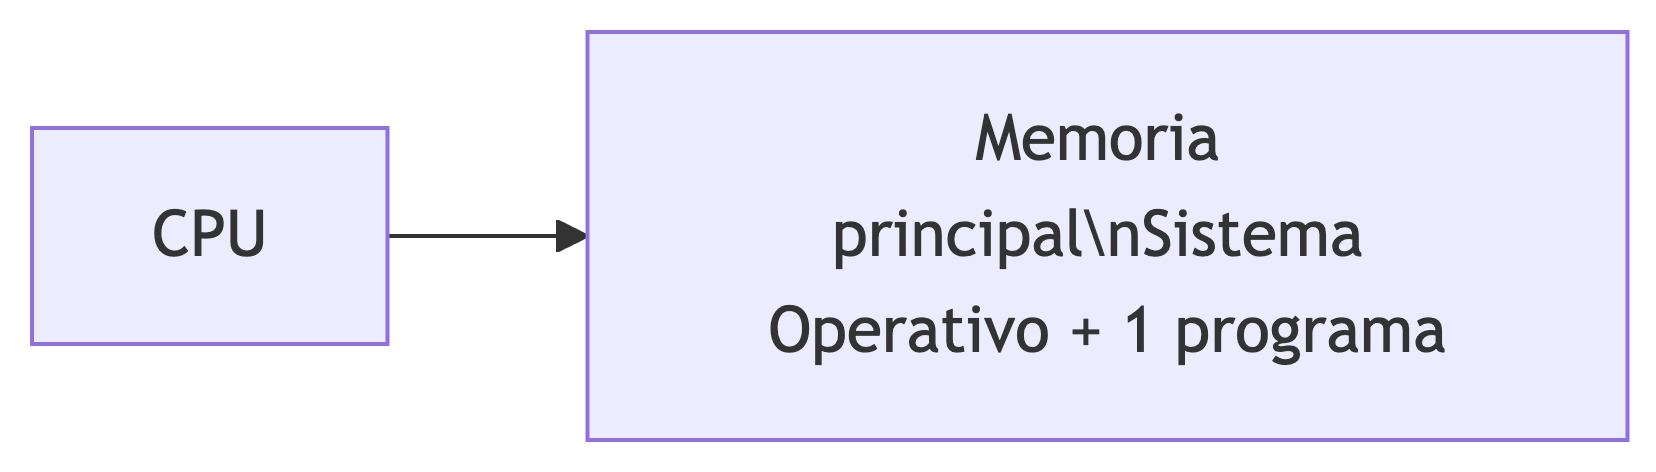
\includegraphics[width=4.32in,height=1.23in]{capitulos/17_gestion_memoria_sistemas_monoprogramados_files/figure-latex/mermaid-figure-1.png}

\begin{quote}
\textbf{Idea clave:} monoprogramación no significa que la computadora no
tenga sistema operativo. Significa que solo hay \textbf{un programa de
usuario en ejecución a la vez}.
\end{quote}

\section{2. ¿Qué es un sistema
monoprogramado?}\label{quuxe9-es-un-sistema-monoprogramado}

En un sistema monoprogramado la memoria puede imaginarse dividida en dos
grandes regiones:

\begin{enumerate}
\def\labelenumi{\arabic{enumi}.}
\tightlist
\item
  Una región reservada para el \textbf{sistema operativo}.
\item
  Una región utilizada por el \textbf{programa de usuario}.
\end{enumerate}

No existe coexistencia de varios programas de usuario compitiendo por la
RAM. El control es mucho más simple que en un sistema multiprogramado.

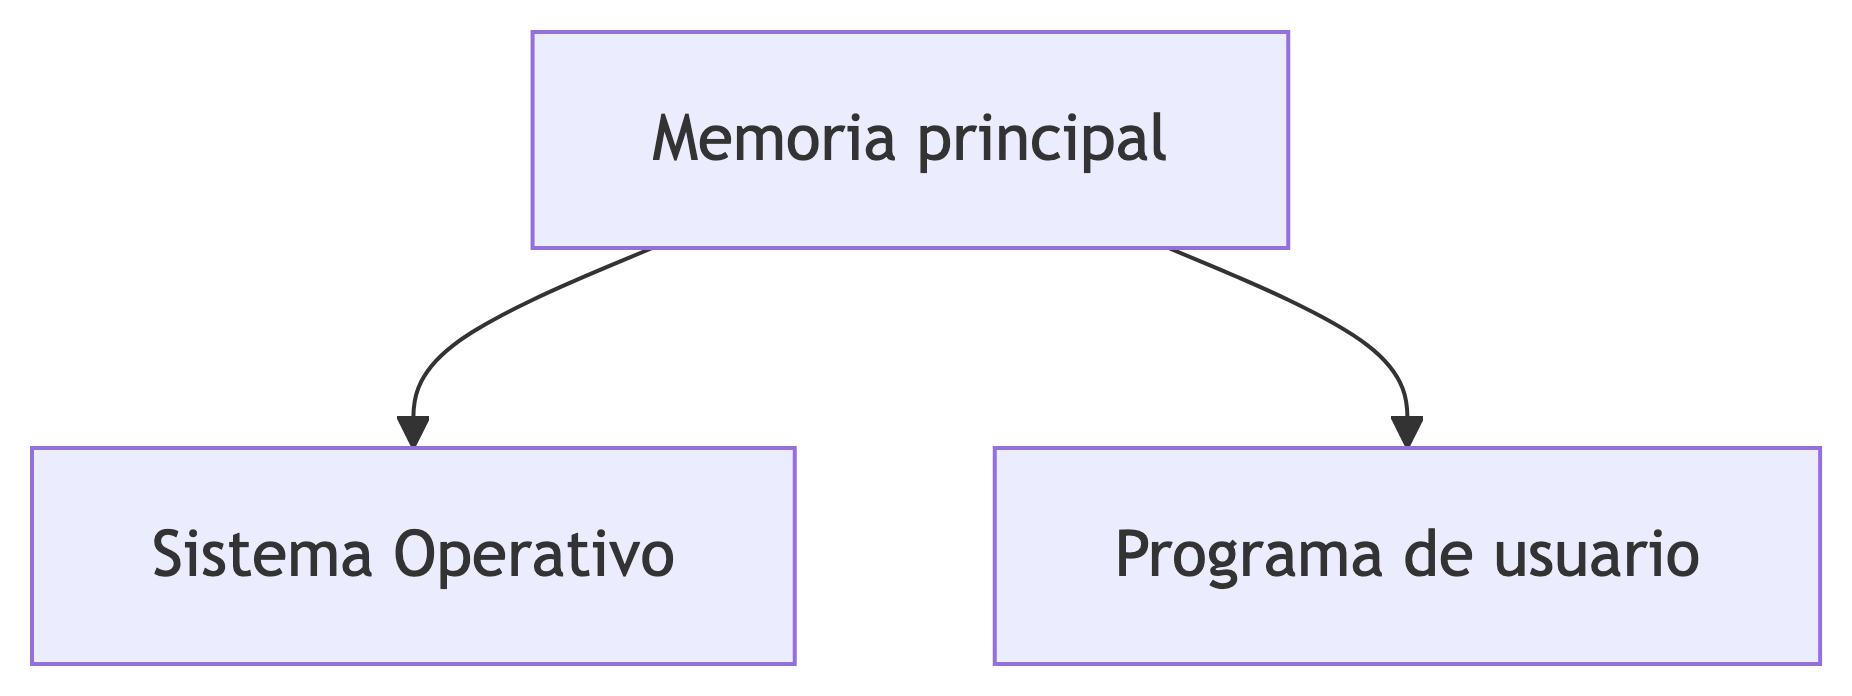
\includegraphics[width=4.82in,height=1.81in]{capitulos/17_gestion_memoria_sistemas_monoprogramados_files/figure-latex/mermaid-figure-7.png}

\subsection{Ejemplo conceptual}\label{ejemplo-conceptual}

Supongamos una memoria de \textbf{512 KB}:

{\def\LTcaptype{none} % do not increment counter
\begin{longtable}[]{@{}
  >{\raggedright\arraybackslash}p{(\linewidth - 4\tabcolsep) * \real{0.3000}}
  >{\raggedleft\arraybackslash}p{(\linewidth - 4\tabcolsep) * \real{0.4000}}
  >{\raggedright\arraybackslash}p{(\linewidth - 4\tabcolsep) * \real{0.3000}}@{}}
\toprule\noalign{}
\begin{minipage}[b]{\linewidth}\raggedright
Región
\end{minipage} & \begin{minipage}[b]{\linewidth}\raggedleft
Tamaño
\end{minipage} & \begin{minipage}[b]{\linewidth}\raggedright
Contenido
\end{minipage} \\
\midrule\noalign{}
\endhead
\bottomrule\noalign{}
\endlastfoot
Sistema operativo & 128 KB & Kernel y componentes residentes \\
Programa de usuario & 300 KB & Código, datos y pila \\
Espacio no utilizado & 84 KB & Memoria disponible que no usa otro
proceso \\
\end{longtable}
}

El espacio libre permanece sin aprovechar por otros programas mientras
se mantiene el modelo monoprogramado.

\section{3. Asignación contigua
simple}\label{asignaciuxf3n-contigua-simple}

La forma más sencilla de cargar el programa consiste en colocarlo en
\textbf{un único bloque continuo de memoria}. A esto se le denomina
\textbf{asignación contigua}.

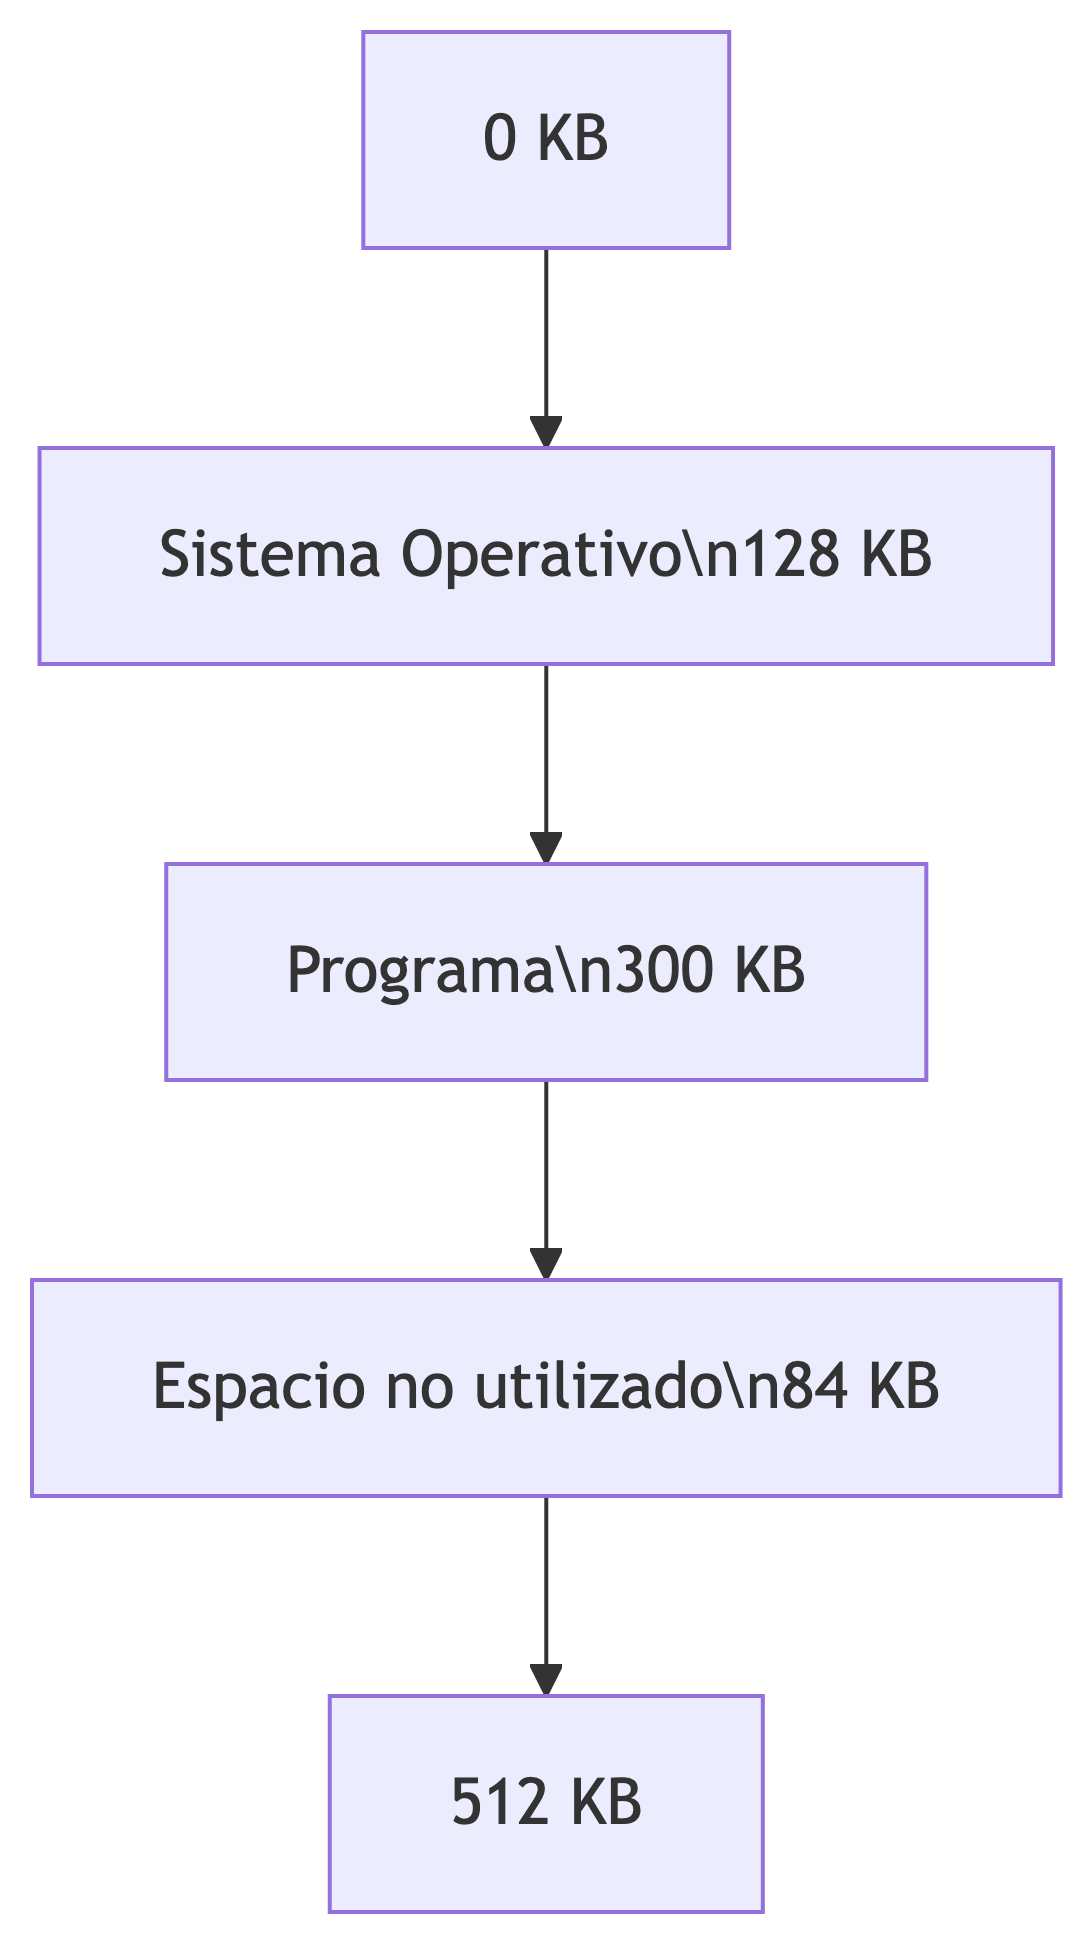
\includegraphics[width=2.85in,height=5.06in]{capitulos/17_gestion_memoria_sistemas_monoprogramados_files/figure-latex/mermaid-figure-6.png}

\subsection{Características}\label{caracteruxedsticas}

\begin{itemize}
\tightlist
\item
  El programa ocupa posiciones consecutivas de memoria.
\item
  Su tamaño no puede superar la memoria disponible para el usuario.
\item
  La administración es sencilla porque solo existe un bloque de programa
  que controlar.
\item
  Si queda memoria libre, no se utiliza para ejecutar simultáneamente
  otro programa.
\end{itemize}

\begin{tcolorbox}[enhanced jigsaw, arc=.35mm, bottomrule=.15mm, bottomtitle=1mm, breakable, colback=white, colbacktitle=quarto-callout-note-color!10!white, colframe=quarto-callout-note-color-frame, coltitle=black, left=2mm, leftrule=.75mm, opacityback=0, opacitybacktitle=0.6, rightrule=.15mm, title=\textcolor{quarto-callout-note-color}{\faInfo}\hspace{0.5em}{Conexión con la siguiente etapa del curso}, titlerule=0mm, toprule=.15mm, toptitle=1mm]

Aquí aparece por primera vez la \textbf{asignación contigua}. Más
adelante, en la Clase 19, estudiaremos esta técnica como un problema
general de administración de memoria y analizaremos algoritmos de
asignación con mayor profundidad.

\end{tcolorbox}

\section{4. Direcciones de memoria}\label{direcciones-de-memoria}

Cuando un programa utiliza una variable o ejecuta una instrucción,
necesita localizarla en memoria. Para comprender este proceso
distinguiremos dos conceptos.

\subsection{Dirección lógica}\label{direcciuxf3n-luxf3gica}

Es la referencia utilizada por el programa antes de considerar su
ubicación física definitiva. Puede verse como una posición relativa
dentro de su propio espacio de direcciones.

\subsection{Dirección física}\label{direcciuxf3n-fuxedsica-1}

Es la posición real que ocupa el dato o instrucción dentro de la memoria
RAM.

{\def\LTcaptype{none} % do not increment counter
\begin{longtable}[]{@{}llr@{}}
\toprule\noalign{}
Tipo & Pregunta que responde & Ejemplo \\
\midrule\noalign{}
\endhead
\bottomrule\noalign{}
\endlastfoot
Lógica & ¿Dónde está dentro del programa? & 250 \\
Física & ¿Dónde está realmente en RAM? & 2250 \\
\end{longtable}
}

\section{5. Direcciones absolutas}\label{direcciones-absolutas}

Una estrategia muy simple consiste en generar \textbf{direcciones
físicas fijas}. En este caso, el programa debe cargarse siempre en la
ubicación para la cual fue preparado.

Si una instrucción espera encontrar un dato en la dirección física 2250,
cambiar el programa de posición sin ajustar sus referencias provocaría
accesos incorrectos.

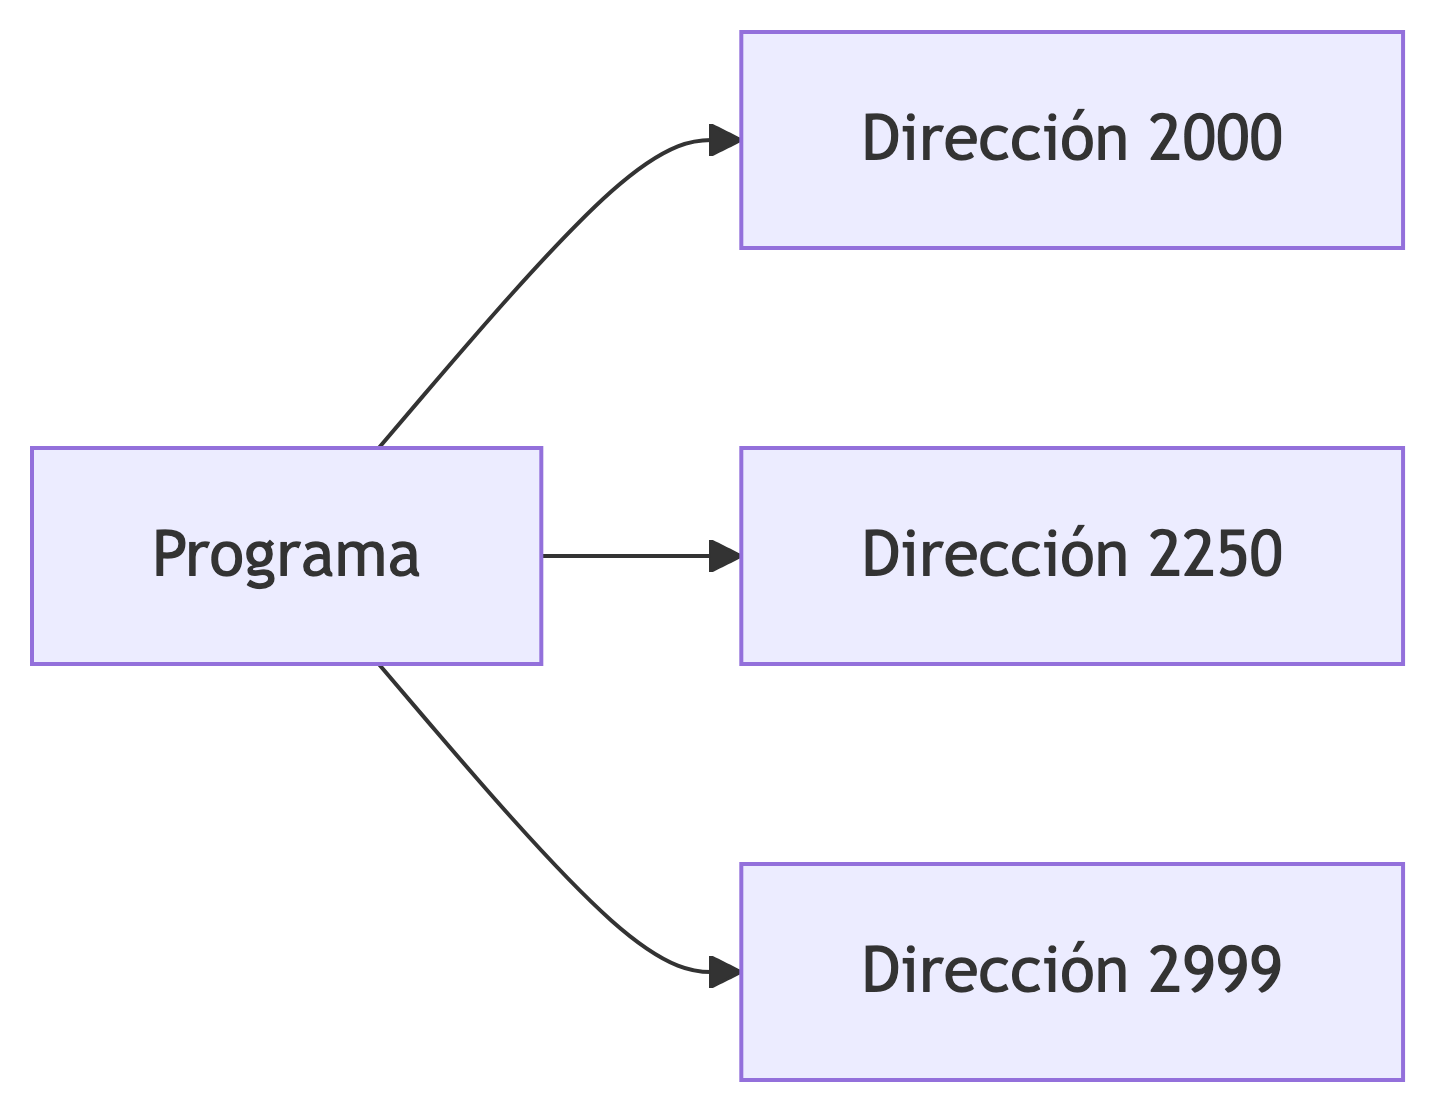
\includegraphics[width=3.74in,height=2.9in]{capitulos/17_gestion_memoria_sistemas_monoprogramados_files/figure-latex/mermaid-figure-5.png}

Este enfoque es sencillo, pero poco flexible.

\section{6. Relocación estática}\label{relocaciuxf3n-estuxe1tica}

Una alternativa consiste en permitir que el programa utilice direcciones
relativas y realizar un ajuste \textbf{una sola vez, durante la carga}.
A este procedimiento lo llamamos \textbf{relocación estática}.

La idea puede expresarse de manera sencilla:

\[
\text{Dirección física} = \text{Dirección base} + \text{Dirección lógica}
\]

\subsection{Ejemplo}\label{ejemplo-8}

El sistema operativo ocupa las direcciones \textbf{0 a 1999} y el
programa utiliza direcciones lógicas \textbf{0 a 999}. El cargador
decide colocar el programa a partir de la dirección \textbf{2000}.

Si el programa solicita su dirección lógica 250:

\[
2000 + 250 = 2250
\]

Por lo tanto, la dirección física correspondiente es \textbf{2250}.

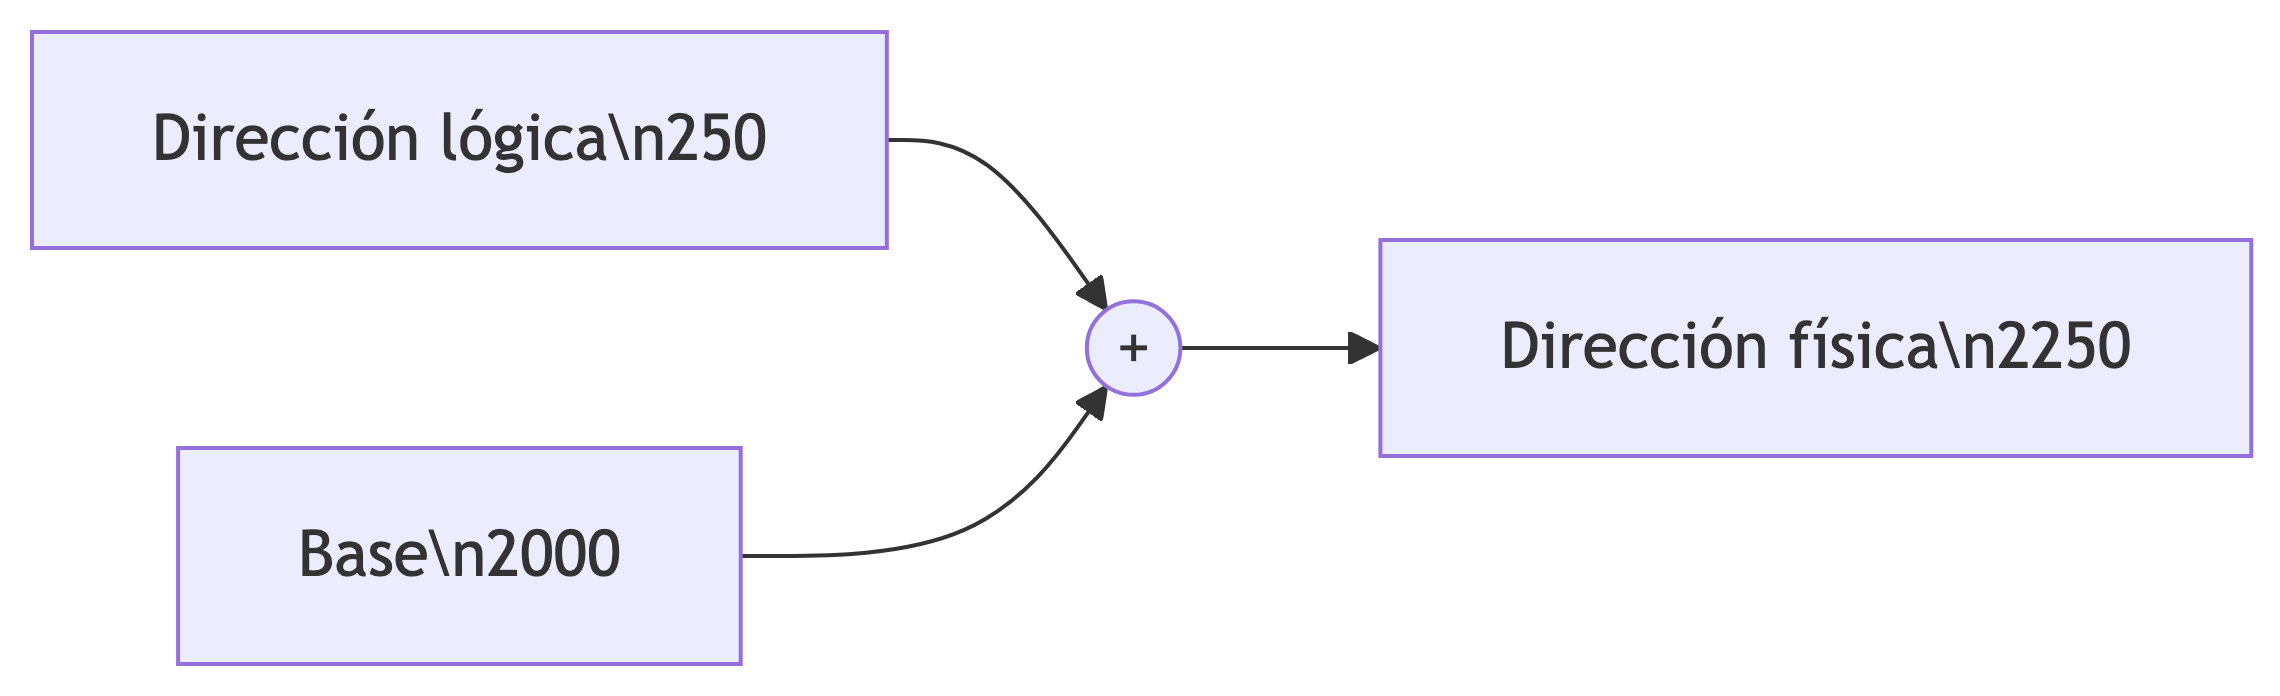
\includegraphics[width=5.95in,height=1.81in]{capitulos/17_gestion_memoria_sistemas_monoprogramados_files/figure-latex/mermaid-figure-4.png}

\begin{tcolorbox}[enhanced jigsaw, arc=.35mm, bottomrule=.15mm, bottomtitle=1mm, breakable, colback=white, colbacktitle=quarto-callout-important-color!10!white, colframe=quarto-callout-important-color-frame, coltitle=black, left=2mm, leftrule=.75mm, opacityback=0, opacitybacktitle=0.6, rightrule=.15mm, title=\textcolor{quarto-callout-important-color}{\faExclamation}\hspace{0.5em}{No confundamos los momentos}, titlerule=0mm, toprule=.15mm, toptitle=1mm]

En la \textbf{relocación estática}, el ajuste se realiza al cargar el
programa. Una vez que comienza su ejecución, el programa permanece en
esa ubicación. En sistemas más avanzados veremos \textbf{relocación
dinámica}, donde la traducción ocurre durante la ejecución.

\end{tcolorbox}

\section{7. Ejemplo en C++: simulando la
relocación}\label{ejemplo-en-c-simulando-la-relocaciuxf3n}

El siguiente programa no administra la RAM real del sistema operativo;
únicamente nos ayuda a representar matemáticamente la traducción base +
desplazamiento.

\begin{Shaded}
\begin{Highlighting}[]
\NormalTok{\#include \textless{}iostream\textgreater{}}
\NormalTok{using namespace std;}

\NormalTok{int main() \{}
\NormalTok{    int base = 2000;}
\NormalTok{    int direccionLogica = 250;}
\NormalTok{    int direccionFisica = base + direccionLogica;}

\NormalTok{    cout \textless{}\textless{} "Direccion fisica: " \textless{}\textless{} direccionFisica \textless{}\textless{} endl;}
\NormalTok{    return 0;}
\NormalTok{\}}
\end{Highlighting}
\end{Shaded}

La salida esperada es:

\begin{Shaded}
\begin{Highlighting}[]
\NormalTok{Direccion fisica: 2250}
\end{Highlighting}
\end{Shaded}

\subsection{Comprueba tu comprensión}\label{comprueba-tu-comprensiuxf3n}

Si la dirección base fuera 4096 y el programa solicitara la dirección
lógica 120, ¿cuál sería la dirección física?

Ver respuesta

\[4096 + 120 = 4216\]

La dirección física sería \textbf{4216}.

\section{8. Protección de memoria: una limitación
importante}\label{protecciuxf3n-de-memoria-una-limitaciuxf3n-importante}

En los modelos monoprogramados más simples la protección puede ser
mínima o inexistente. Si un programa escribe fuera del espacio que le
corresponde, podría modificar memoria reservada para el sistema
operativo.

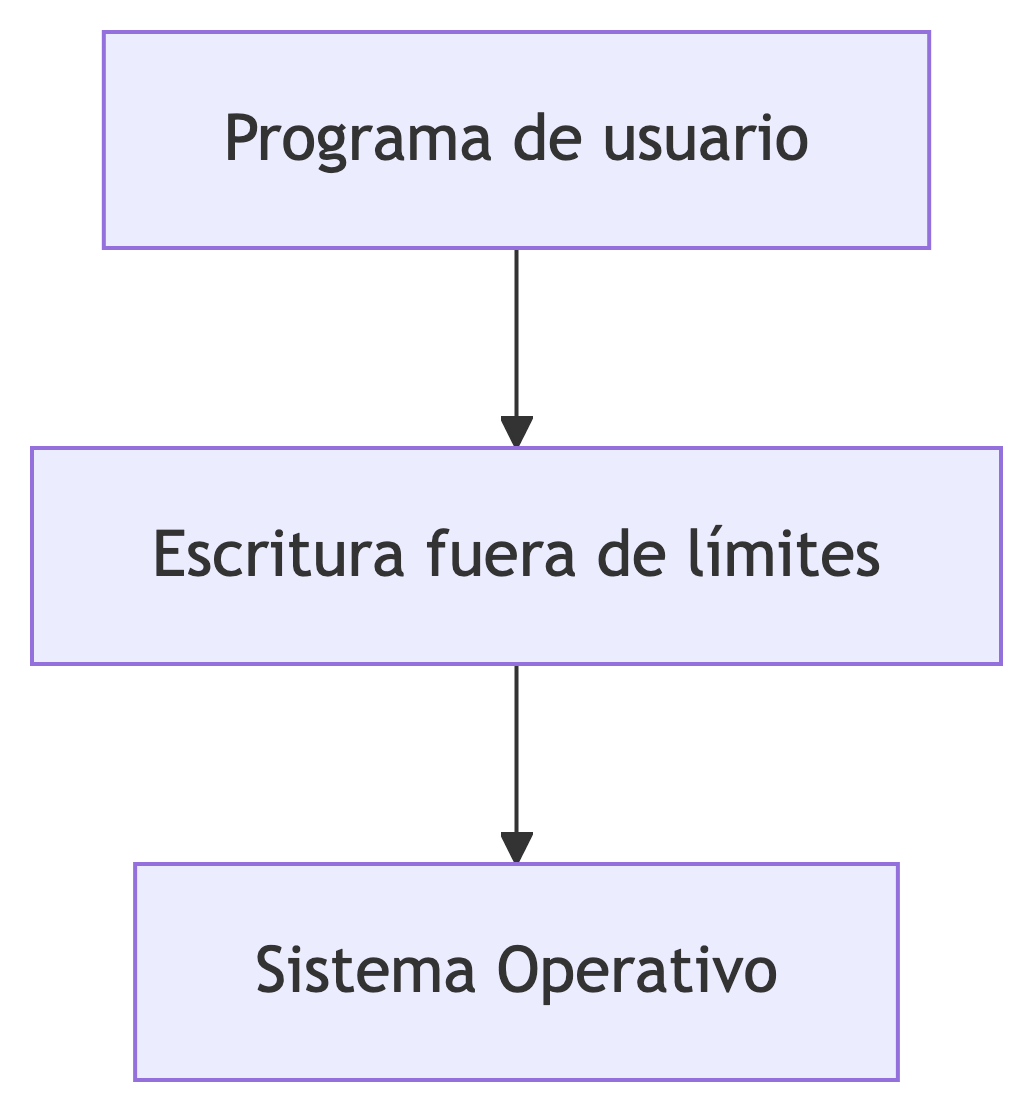
\includegraphics[width=2.69in,height=2.9in]{capitulos/17_gestion_memoria_sistemas_monoprogramados_files/figure-latex/mermaid-figure-3.png}

Esto ayuda a comprender por qué la \textbf{protección de memoria} se
convirtió en una responsabilidad fundamental de los sistemas operativos
posteriores.

\section{9. Ventajas y limitaciones}\label{ventajas-y-limitaciones}

{\def\LTcaptype{none} % do not increment counter
\begin{longtable}[]{@{}
  >{\raggedright\arraybackslash}p{(\linewidth - 2\tabcolsep) * \real{0.5000}}
  >{\raggedright\arraybackslash}p{(\linewidth - 2\tabcolsep) * \real{0.5000}}@{}}
\toprule\noalign{}
\begin{minipage}[b]{\linewidth}\raggedright
Ventajas
\end{minipage} & \begin{minipage}[b]{\linewidth}\raggedright
Limitaciones
\end{minipage} \\
\midrule\noalign{}
\endhead
\bottomrule\noalign{}
\endlastfoot
Diseño sencillo & Solo un programa de usuario a la vez \\
Administración de memoria simple & No aprovecha la RAM libre para
ejecutar otros programas \\
Poco trabajo de administración & Flexibilidad limitada para mover
programas \\
Adecuado para tareas dedicadas & Protección limitada en implementaciones
simples \\
\end{longtable}
}

\section{10. Un ejemplo cercano: sistemas
dedicados}\label{un-ejemplo-cercano-sistemas-dedicados}

El principio de ejecutar una única aplicación principal sigue siendo
útil para comprender ciertos \textbf{sistemas embebidos y dispositivos
dedicados}. Sin embargo, no debemos asumir que todo microcontrolador
moderno carece de concurrencia o de un sistema operativo: algunos
incorporan planificadores o sistemas operativos en tiempo real.

La idea importante para esta clase es el \textbf{modelo conceptual}: una
tarea principal, una organización sencilla de memoria y ausencia de
varios programas de usuario residentes simultáneamente.

\section{11. Actividad guiada}\label{actividad-guiada}

Una computadora dispone de \textbf{1 MB = 1024 KB} de memoria principal.

\begin{itemize}
\tightlist
\item
  Sistema operativo: 256 KB
\item
  Programa de usuario: 500 KB
\end{itemize}

Responde:

\begin{enumerate}
\def\labelenumi{\arabic{enumi}.}
\tightlist
\item
  ¿Cuánta memoria queda sin utilizar?
\item
  Dibuja la distribución de memoria.
\item
  Si el programa comienza en la dirección 256 KB, ¿qué representa esa
  posición?
\item
  ¿Podría cargarse simultáneamente otro programa de 200 KB manteniendo
  estrictamente el modelo monoprogramado? Explica.
\end{enumerate}

\subsection{Solución de la parte
numérica}\label{soluciuxf3n-de-la-parte-numuxe9rica}

\[
1024 - 256 - 500 = 268\text{ KB}
\]

Quedan \textbf{268 KB} sin utilizar.

\begin{quote}
\textbf{Atención:} si se considera 1 MB como 1000 KB se obtendrían 244
KB, pero en este ejercicio trabajaremos con \textbf{1 MB = 1024 KB} para
mantener consistencia binaria.
\end{quote}

\section{12. Reto de análisis}\label{reto-de-anuxe1lisis}

Un programa utiliza direcciones lógicas de 0 a 1499. El sistema
operativo ocupa las direcciones físicas 0 a 4095 y el programa se carga
inmediatamente después.

\begin{enumerate}
\def\labelenumi{\arabic{enumi}.}
\tightlist
\item
  ¿Cuál es la dirección base del programa?
\item
  ¿Cuál es la dirección física correspondiente a la dirección lógica
  300?
\item
  ¿Cuál es la última dirección física que podría utilizar el programa?
\item
  ¿Qué tendría que ocurrir con las referencias del programa si se
  cargara en otra ubicación usando relocación estática?
\end{enumerate}

\section{13. Del sistema monoprogramado al
multiprogramado}\label{del-sistema-monoprogramado-al-multiprogramado}

El gran problema del modelo estudiado aparece cuando el programa se
detiene esperando una operación de entrada/salida: la CPU podría quedar
sin trabajo aunque exista memoria disponible.

Esto conduce a una pregunta natural:

\begin{quote}
\textbf{¿Por qué no mantener varios procesos en memoria y permitir que
la CPU trabaje con otro mientras uno espera?}
\end{quote}

Esa pregunta nos lleva directamente a la \textbf{Clase 18: Gestión de
Memoria en Sistemas Multiprogramados}.

\section{14. Resumen}\label{resumen-1}

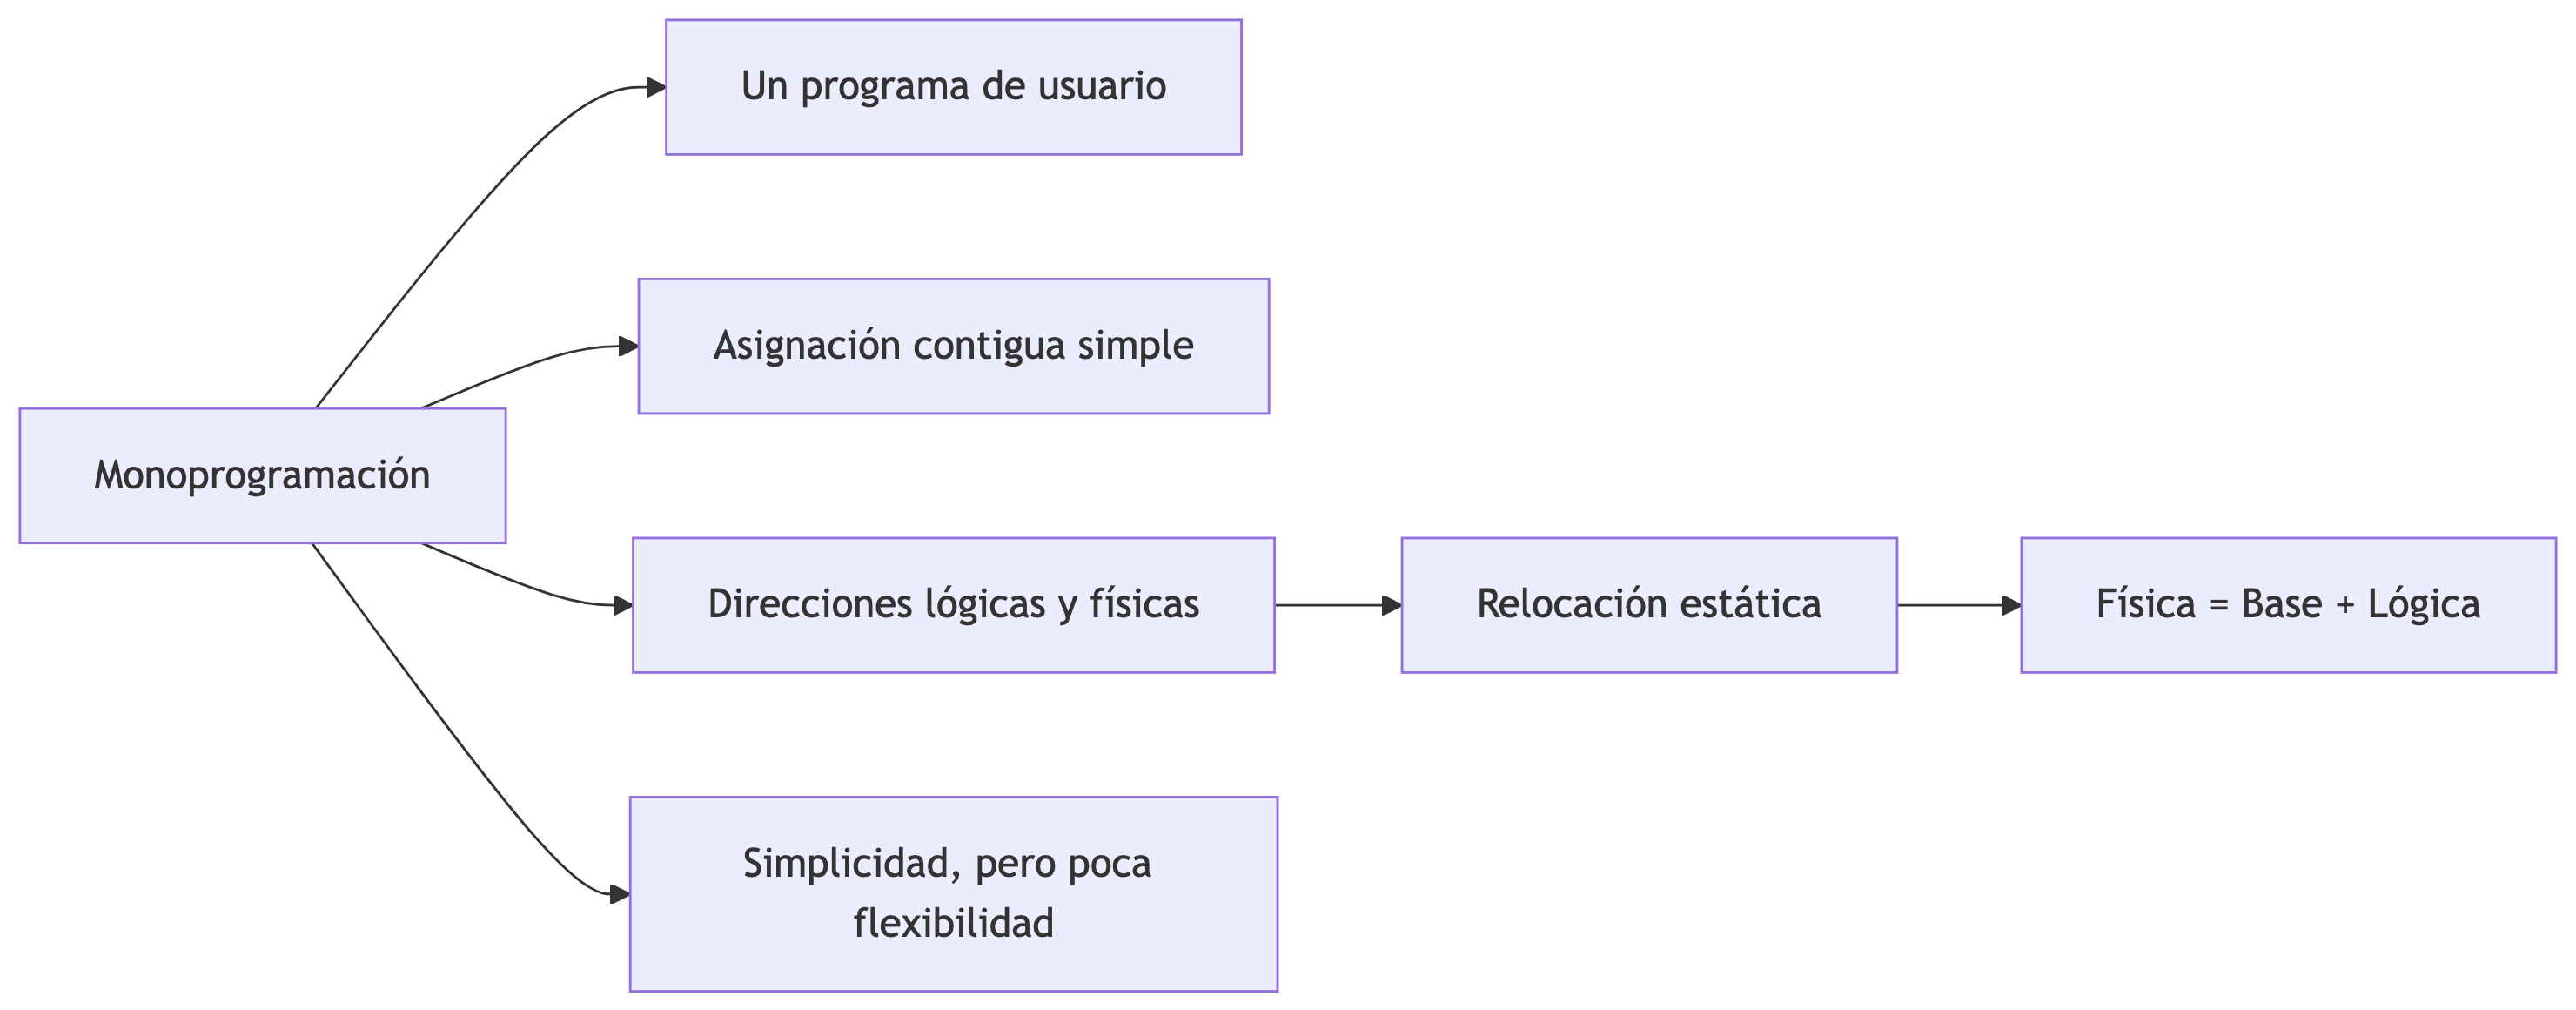
\includegraphics[width=10.78in,height=4.23in]{capitulos/17_gestion_memoria_sistemas_monoprogramados_files/figure-latex/mermaid-figure-2.png}

\subsection{Lo que debes llevarte de esta
clase}\label{lo-que-debes-llevarte-de-esta-clase}

\begin{itemize}
\tightlist
\item
  La monoprogramación mantiene un único programa de usuario en memoria.
\item
  El programa puede ocupar un bloque contiguo de RAM.
\item
  Una dirección lógica representa una posición desde la perspectiva del
  programa; la dirección física es su ubicación real en RAM.
\item
  La relocación estática ajusta las direcciones al momento de cargar el
  programa.
\item
  La simplicidad del modelo tiene un costo: menor aprovechamiento de CPU
  y memoria y poca flexibilidad.
\end{itemize}

\section{15. Preguntas de
autoevaluación}\label{preguntas-de-autoevaluaciuxf3n}

\begin{enumerate}
\def\labelenumi{\arabic{enumi}.}
\tightlist
\item
  ¿Qué caracteriza a un sistema monoprogramado?
\item
  ¿Cómo se organiza típicamente su memoria?
\item
  ¿Qué significa que la asignación sea contigua?
\item
  ¿Cuál es la diferencia entre dirección lógica y física?
\item
  ¿Qué es una dirección absoluta?
\item
  ¿En qué momento ocurre la relocación estática?
\item
  Si la base es 3000 y la dirección lógica es 450, ¿cuál es la dirección
  física?
\item
  ¿Por qué puede desperdiciarse memoria en este modelo?
\item
  ¿Qué riesgo existe si no hay protección de memoria?
\item
  ¿Qué necesidad tecnológica conduce de la monoprogramación a la
  multiprogramación?
\end{enumerate}

\bookmarksetup{startatroot}

\chapter{Gestión de Memoria en Sistemas
Multiprogramados}\label{gestiuxf3n-de-memoria-en-sistemas-multiprogramados}

Clase No. 18 - Sistemas Operativos I

\hfill\break

\bookmarksetup{startatroot}

\chapter{Gestión de Memoria en Sistemas
Multiprogramados}\label{gestiuxf3n-de-memoria-en-sistemas-multiprogramados-1}

\section{¿Qué aprenderemos en esta
clase?}\label{quuxe9-aprenderemos-en-esta-clase-1}

Al finalizar este capítulo, el estudiante será capaz de:

\begin{itemize}
\tightlist
\item
  Explicar por qué la multiprogramación mejora el aprovechamiento de la
  CPU.
\item
  Diferenciar particiones fijas y particiones dinámicas.
\item
  Distinguir fragmentación interna de fragmentación externa.
\item
  Aplicar conceptualmente First Fit, Best Fit y Worst Fit.
\item
  Explicar la compactación y el swapping.
\item
  Comprender el propósito de la protección, la relocación dinámica y la
  MMU.
\item
  Explicar el uso básico de memoria compartida entre procesos.
\end{itemize}

\begin{tcolorbox}[enhanced jigsaw, arc=.35mm, bottomrule=.15mm, bottomtitle=1mm, breakable, colback=white, colbacktitle=quarto-callout-tip-color!10!white, colframe=quarto-callout-tip-color-frame, coltitle=black, left=2mm, leftrule=.75mm, opacityback=0, opacitybacktitle=0.6, rightrule=.15mm, title=\textcolor{quarto-callout-tip-color}{\faLightbulb}\hspace{0.5em}{Tres preguntas fundamentales}, titlerule=0mm, toprule=.15mm, toptitle=1mm]

\begin{enumerate}
\def\labelenumi{\arabic{enumi}.}
\tightlist
\item
  ¿Cómo podemos mantener varios procesos en memoria sin que interfieran
  entre sí?
\item
  ¿Qué hacemos cuando el espacio libre existe, pero está dividido en
  pequeños huecos?
\item
  ¿Cómo puede un proceso usar direcciones lógicas sin conocer su
  posición física exacta?
\end{enumerate}

\end{tcolorbox}

\section{1. El problema que dejó la
monoprogramación}\label{el-problema-que-dejuxf3-la-monoprogramaciuxf3n}

En la Clase 17 vimos un sistema con un único programa de usuario en
memoria. Ese modelo es sencillo, pero tiene una limitación importante:
cuando el programa espera una operación de entrada/salida, la CPU puede
quedar ociosa.

La \textbf{multiprogramación} propone mantener \textbf{varios procesos
residentes en memoria al mismo tiempo}. Cuando uno espera, otro puede
utilizar la CPU.

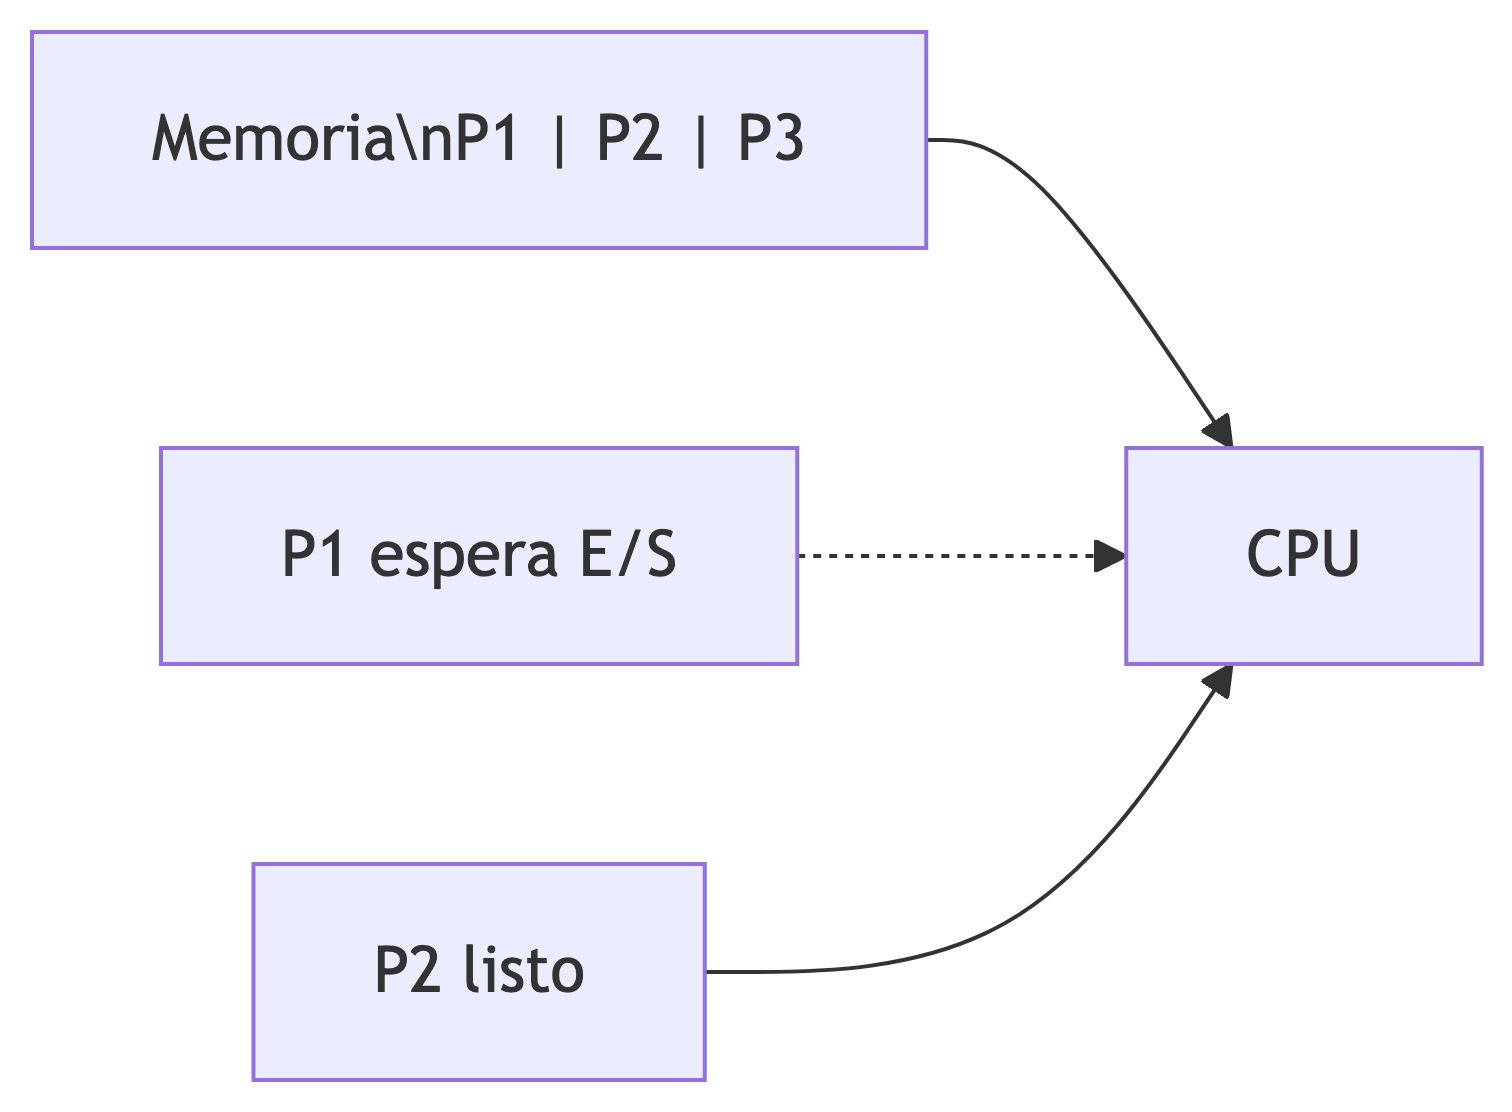
\includegraphics[width=3.94in,height=2.9in]{capitulos/18_gestion_memoria_sistemas_multiprogramados_files/figure-latex/mermaid-figure-1.png}

\begin{quote}
\textbf{Idea clave:} tener varios procesos en memoria no significa que
una sola CPU ejecute todas sus instrucciones exactamente al mismo
instante. Significa que el sistema puede alternar entre procesos y
aprovechar mejor el procesador.
\end{quote}

\section{2. Evolución conceptual}\label{evoluciuxf3n-conceptual}

Podemos entender la evolución de la administración de memoria como una
respuesta a nuevas necesidades:

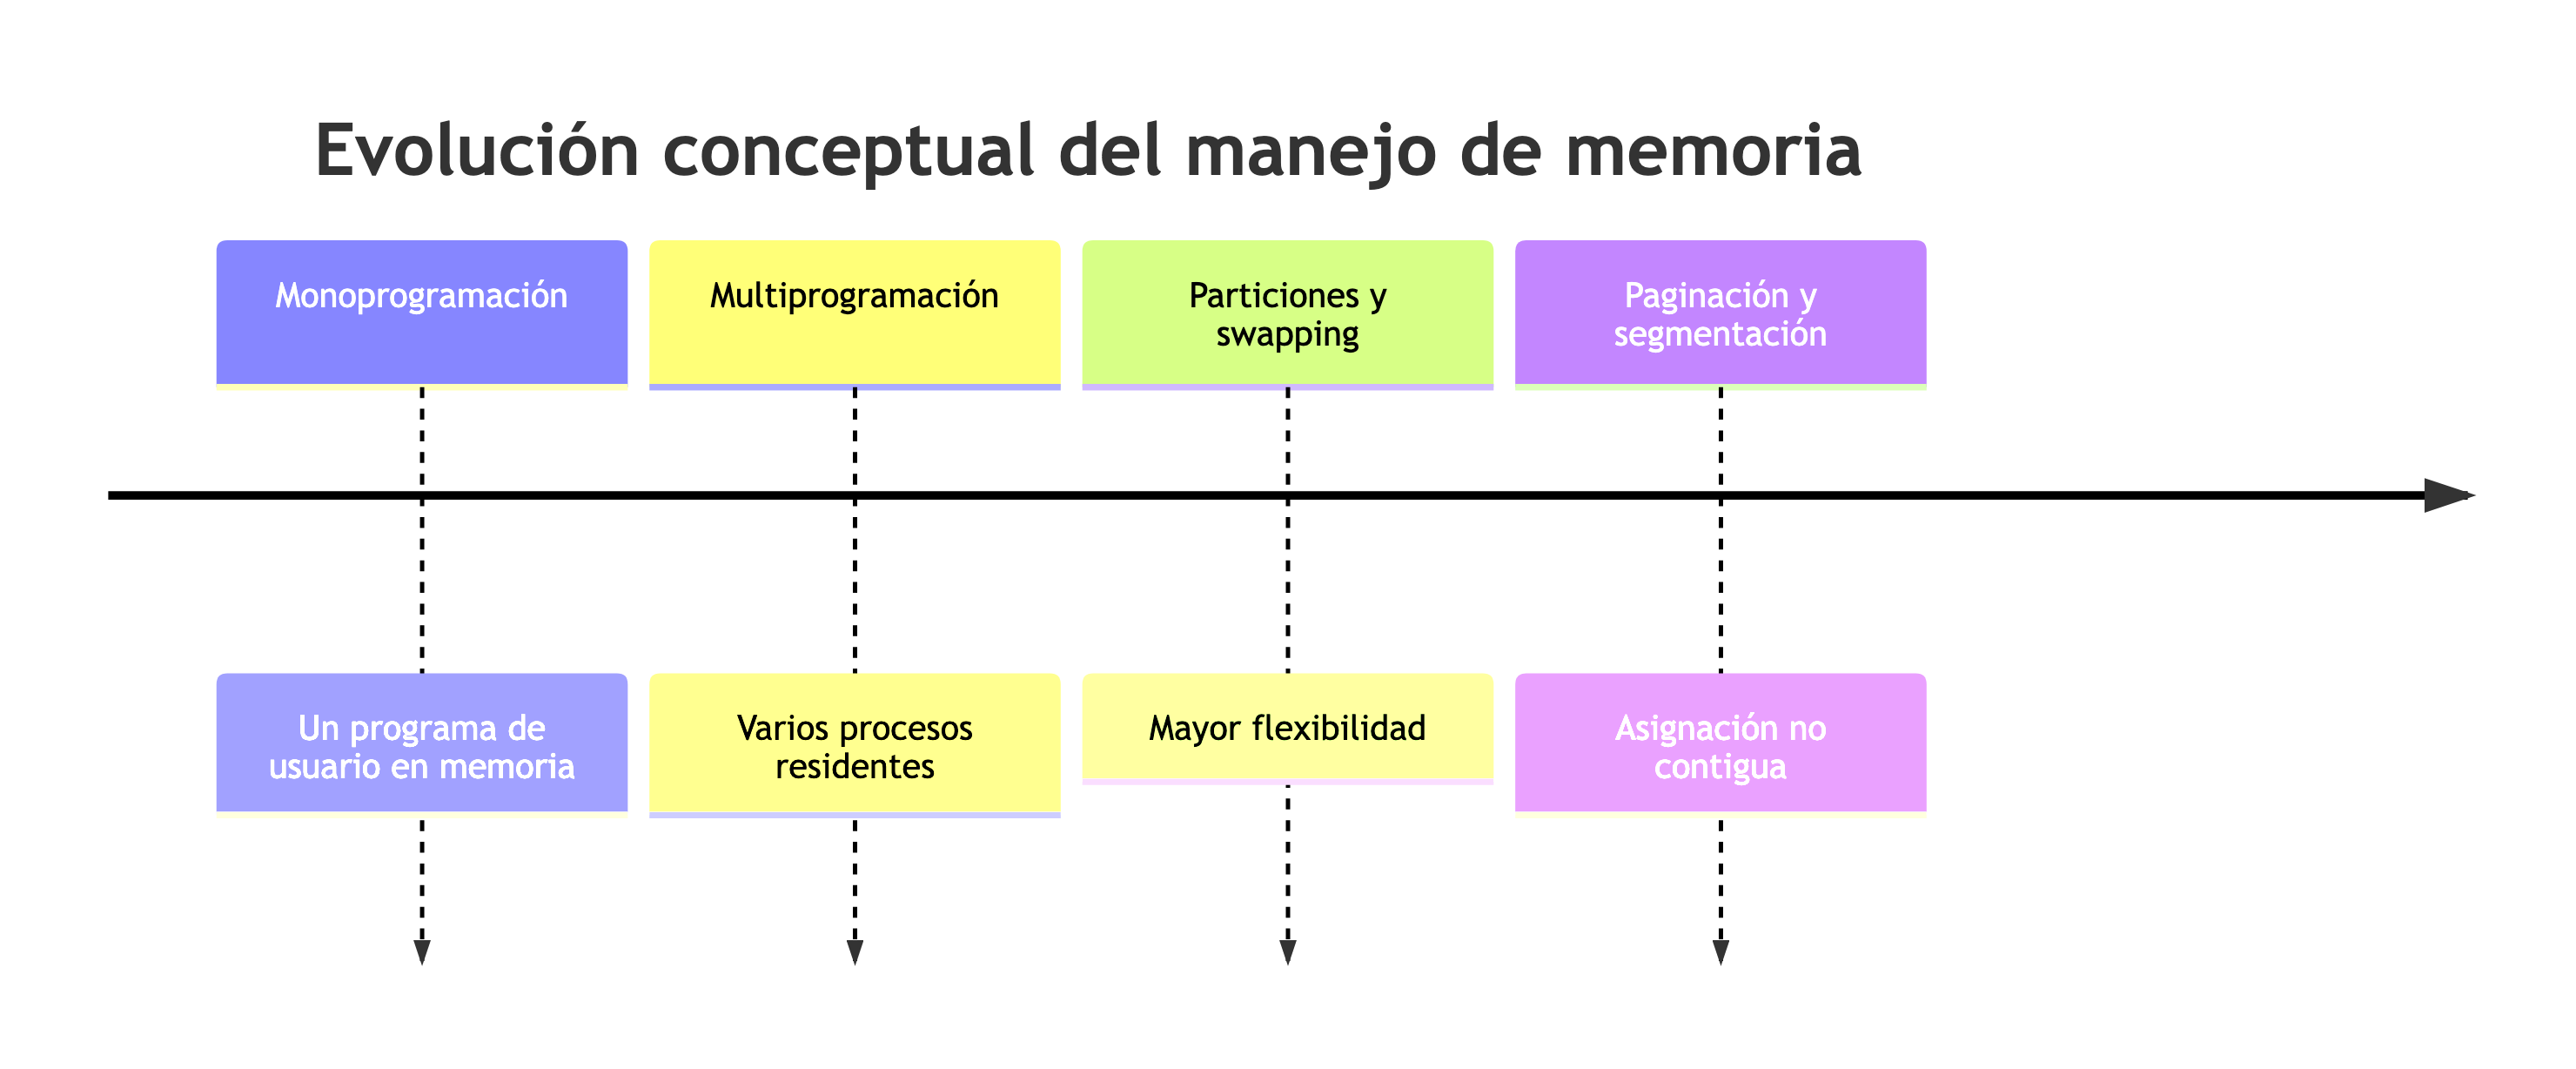
\includegraphics[width=12.4in,height=5.15in]{capitulos/18_gestion_memoria_sistemas_multiprogramados_files/figure-latex/mermaid-figure-11.png}

En esta clase nos concentraremos en la \textbf{multiprogramación
mediante particiones}, el intercambio de procesos y los mecanismos
necesarios para proteger y reubicar programas.

\section{3. Asignación contigua en
multiprogramación}\label{asignaciuxf3n-contigua-en-multiprogramaciuxf3n}

Una primera solución consiste en mantener varios procesos en memoria,
pero exigir que \textbf{cada proceso ocupe un bloque contiguo} de
direcciones físicas.

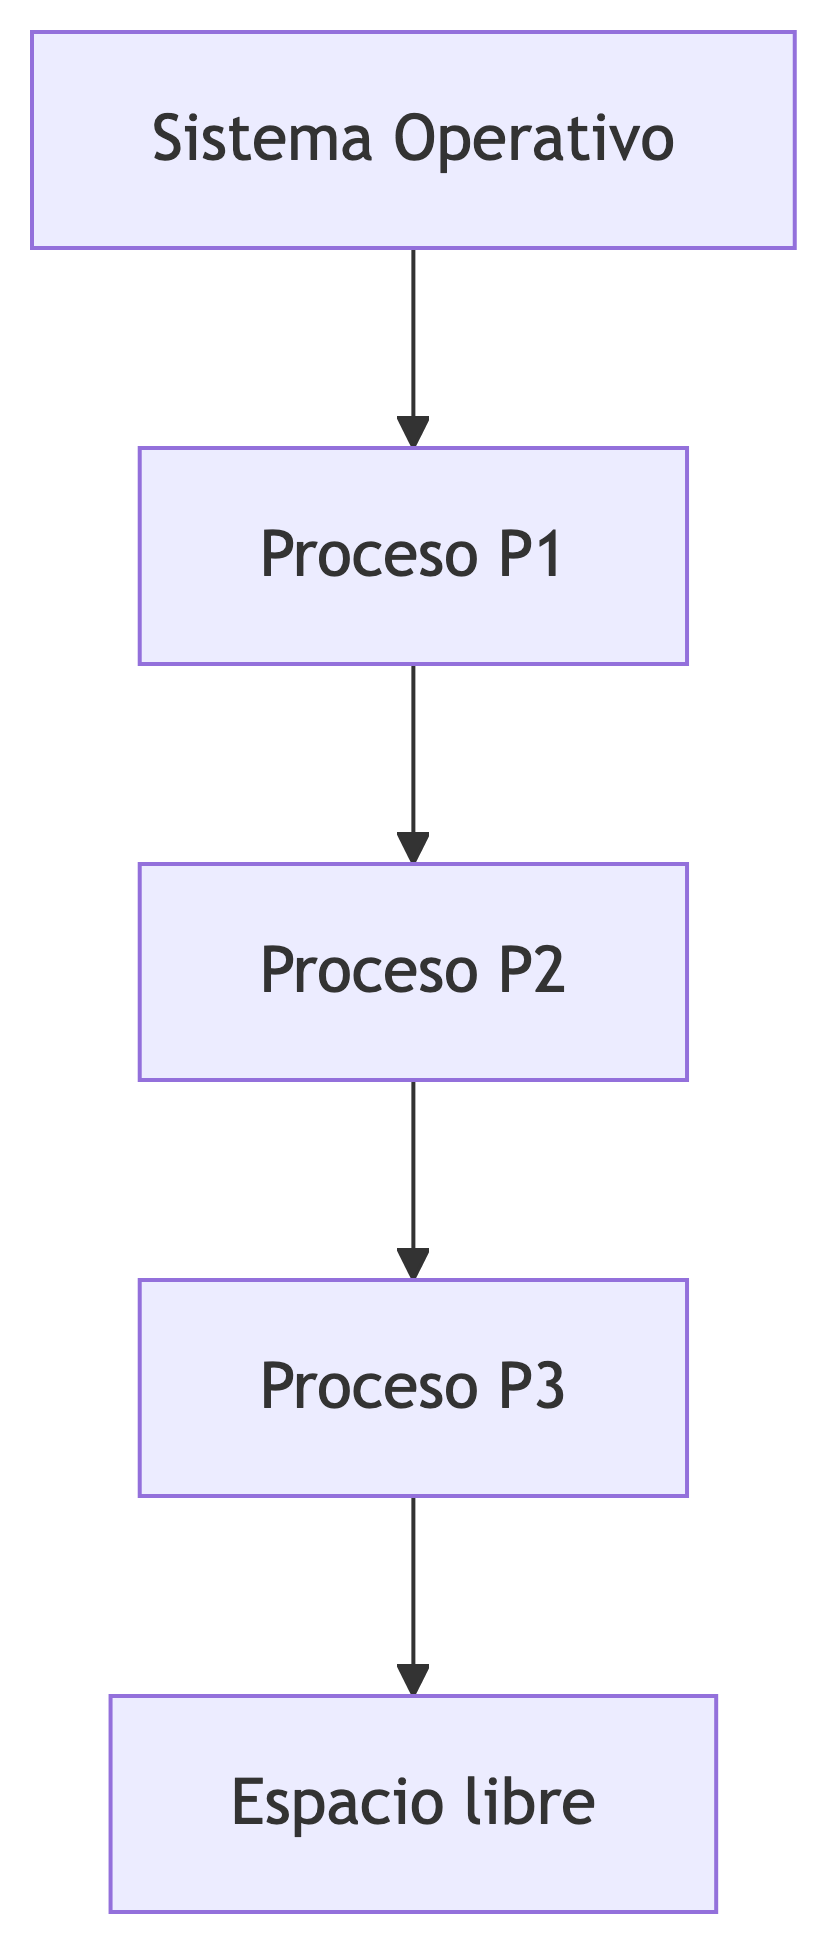
\includegraphics[width=2.15in,height=5.06in]{capitulos/18_gestion_memoria_sistemas_multiprogramados_files/figure-latex/mermaid-figure-10.png}

El reto ya no es solamente cargar un programa, sino decidir \textbf{cómo
dividir la memoria disponible entre varios procesos}.

\section{4. Particiones fijas}\label{particiones-fijas-1}

En las \textbf{particiones fijas}, la memoria se divide previamente en
bloques de tamaño determinado. Cada proceso se coloca en una partición
capaz de contenerlo.

\subsection{Ejemplo}\label{ejemplo-9}

Tenemos tres particiones de 100 KB:

{\def\LTcaptype{none} % do not increment counter
\begin{longtable}[]{@{}
  >{\raggedright\arraybackslash}p{(\linewidth - 8\tabcolsep) * \real{0.1667}}
  >{\raggedleft\arraybackslash}p{(\linewidth - 8\tabcolsep) * \real{0.2222}}
  >{\raggedright\arraybackslash}p{(\linewidth - 8\tabcolsep) * \real{0.1667}}
  >{\raggedleft\arraybackslash}p{(\linewidth - 8\tabcolsep) * \real{0.2222}}
  >{\raggedleft\arraybackslash}p{(\linewidth - 8\tabcolsep) * \real{0.2222}}@{}}
\toprule\noalign{}
\begin{minipage}[b]{\linewidth}\raggedright
Partición
\end{minipage} & \begin{minipage}[b]{\linewidth}\raggedleft
Tamaño
\end{minipage} & \begin{minipage}[b]{\linewidth}\raggedright
Proceso
\end{minipage} & \begin{minipage}[b]{\linewidth}\raggedleft
Tamaño del proceso
\end{minipage} & \begin{minipage}[b]{\linewidth}\raggedleft
Espacio no utilizado dentro de la partición
\end{minipage} \\
\midrule\noalign{}
\endhead
\bottomrule\noalign{}
\endlastfoot
1 & 100 KB & P1 & 80 KB & 20 KB \\
2 & 100 KB & P2 & 90 KB & 10 KB \\
3 & 100 KB & P3 & 50 KB & 50 KB \\
\end{longtable}
}

Aunque los procesos utilizan 220 KB, las tres particiones ocupan 300 KB.
Dentro de ellas quedan \textbf{80 KB que no pueden aprovecharse para
otro proceso}.

\subsection{Fragmentación interna}\label{fragmentaciuxf3n-interna-2}

Ese espacio desperdiciado \textbf{dentro de una región ya asignada}
recibe el nombre de \textbf{fragmentación interna}.

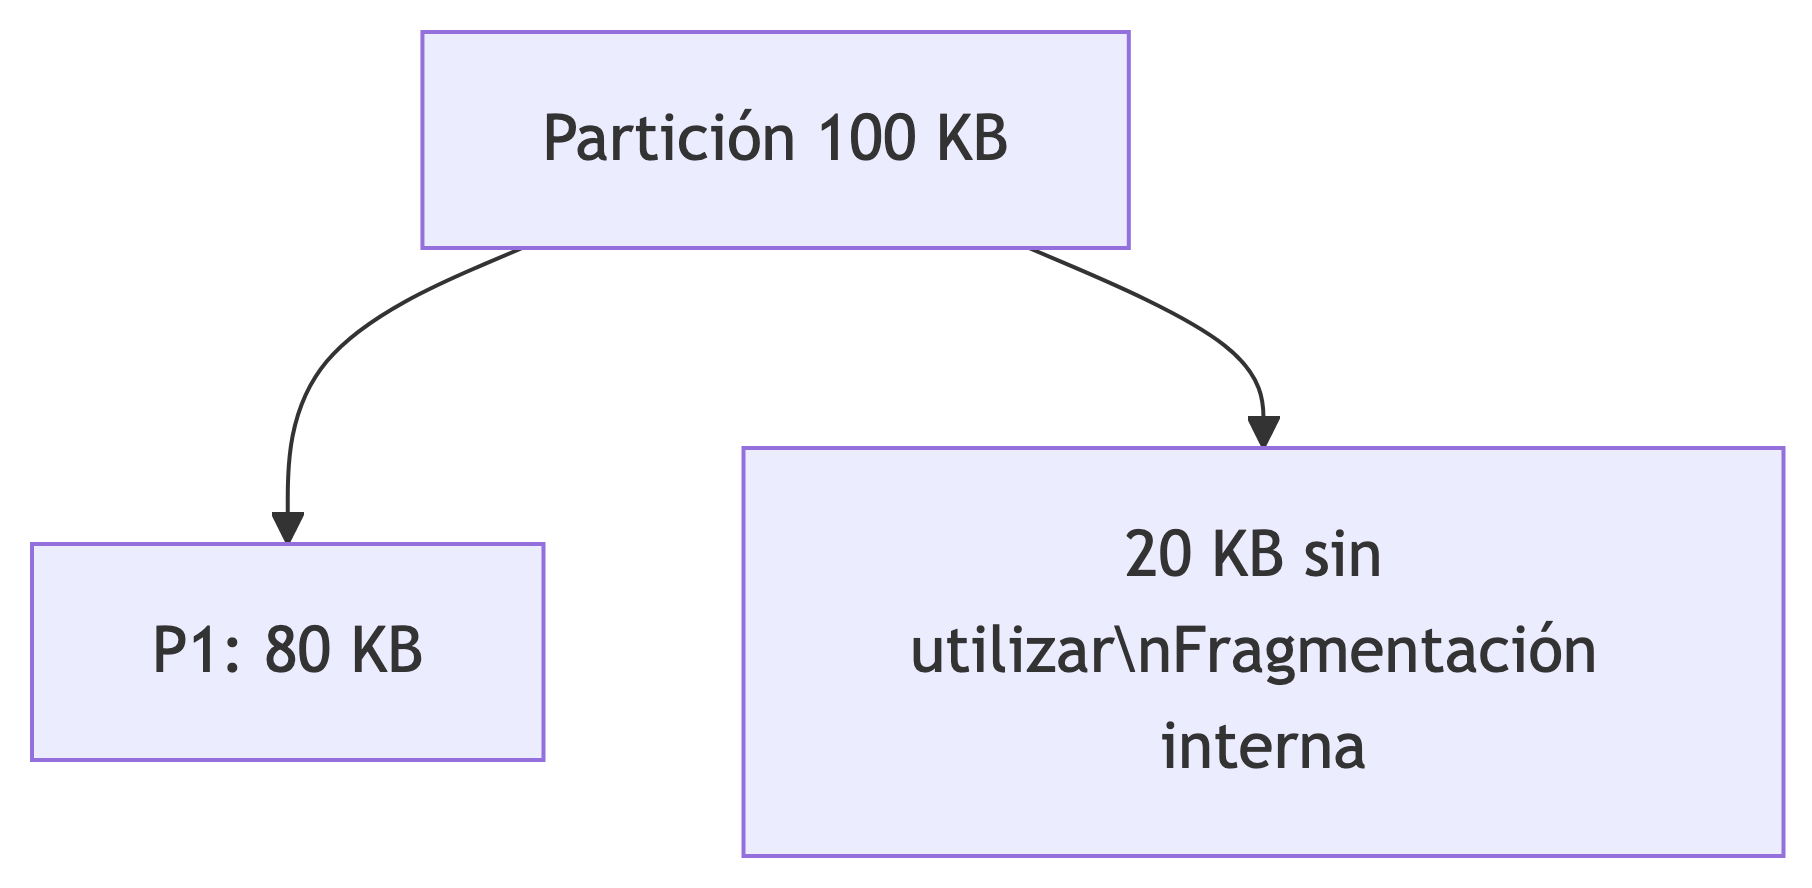
\includegraphics[width=4.73in,height=2.31in]{capitulos/18_gestion_memoria_sistemas_multiprogramados_files/figure-latex/mermaid-figure-9.png}

\section{5. Particiones dinámicas}\label{particiones-dinuxe1micas-1}

En las \textbf{particiones dinámicas}, el sistema crea un bloque de
memoria aproximadamente del tamaño que necesita cada proceso conforme
este llega.

Ejemplo de distribución:

{\def\LTcaptype{none} % do not increment counter
\begin{longtable}[]{@{}lr@{}}
\toprule\noalign{}
Bloque & Tamaño \\
\midrule\noalign{}
\endhead
\bottomrule\noalign{}
\endlastfoot
P1 & 120 KB \\
Libre & 30 KB \\
P2 & 200 KB \\
Libre & 10 KB \\
P3 & 80 KB \\
P4 & 150 KB \\
\end{longtable}
}

Este enfoque reduce el desperdicio dentro de las particiones, pero
introduce otro problema.

\section{6. Fragmentación externa}\label{fragmentaciuxf3n-externa-3}

Con el tiempo, los procesos terminan, entran nuevos procesos y aparecen
\textbf{huecos libres dispersos} entre regiones ocupadas.

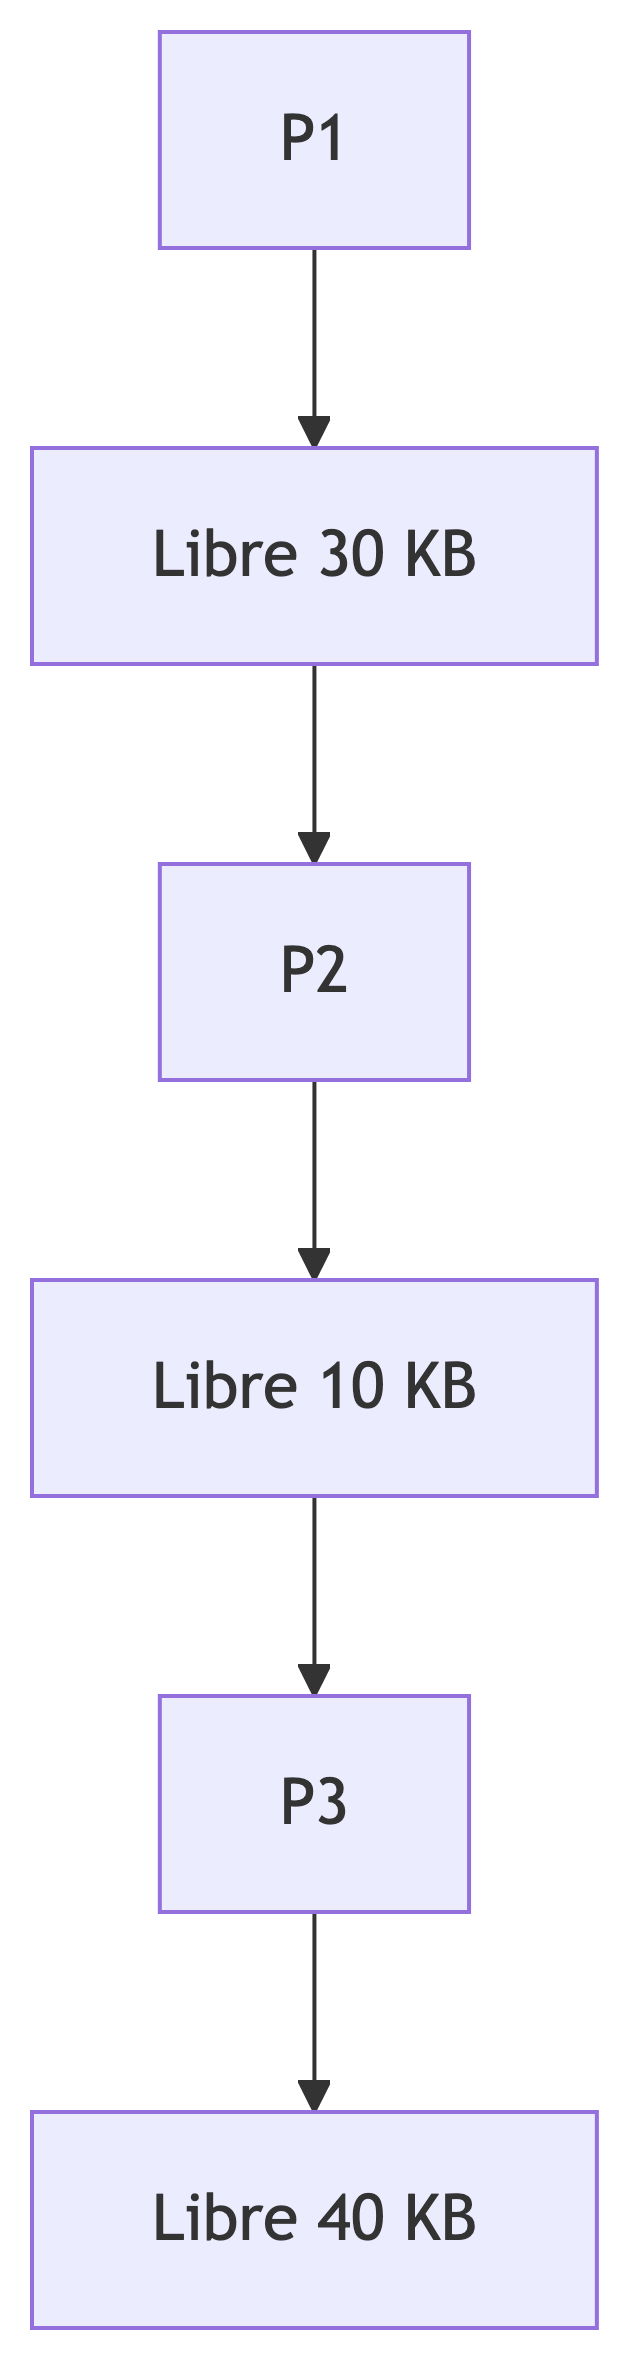
\includegraphics[width=1.64in,height=6.15in]{capitulos/18_gestion_memoria_sistemas_multiprogramados_files/figure-latex/mermaid-figure-8.png}

Supongamos que necesitamos cargar un proceso de \textbf{60 KB}. En total
existen 80 KB libres, pero ningún hueco individual alcanza 60 KB. Como
el proceso necesita un bloque contiguo, \textbf{no puede cargarse}.

A esto lo llamamos \textbf{fragmentación externa}.

\begin{tcolorbox}[enhanced jigsaw, arc=.35mm, bottomrule=.15mm, bottomtitle=1mm, breakable, colback=white, colbacktitle=quarto-callout-important-color!10!white, colframe=quarto-callout-important-color-frame, coltitle=black, left=2mm, leftrule=.75mm, opacityback=0, opacitybacktitle=0.6, rightrule=.15mm, title=\textcolor{quarto-callout-important-color}{\faExclamation}\hspace{0.5em}{Diferencia fundamental}, titlerule=0mm, toprule=.15mm, toptitle=1mm]

\begin{itemize}
\tightlist
\item
  \textbf{Fragmentación interna:} el desperdicio queda \emph{dentro} de
  un bloque asignado.
\item
  \textbf{Fragmentación externa:} el espacio libre queda \emph{fuera} de
  los procesos, pero dividido en huecos dispersos.
\end{itemize}

\end{tcolorbox}

\section{7. ¿Dónde colocar un nuevo
proceso?}\label{duxf3nde-colocar-un-nuevo-proceso}

Cuando existen varios huecos libres, el sistema necesita decidir cuál
utilizar. Tres estrategias clásicas son \textbf{First Fit, Best Fit y
Worst Fit}.

\subsection{First Fit}\label{first-fit-5}

Recorre la memoria desde el inicio y utiliza \textbf{el primer hueco
suficientemente grande}.

\subsection{Best Fit}\label{best-fit-5}

Busca entre los huecos disponibles y utiliza \textbf{el hueco más
pequeño que sea suficientemente grande} para el proceso.

\subsection{Worst Fit}\label{worst-fit-3}

Utiliza \textbf{el hueco libre más grande}, esperando dejar un remanente
todavía aprovechable.

\begin{quote}
\textbf{Corrección conceptual importante:} Best Fit no elige el espacio
más grande; elige el \textbf{menor espacio que todavía permite alojar el
proceso}.
\end{quote}

\section{8. Ejercicio de algoritmos de
ajuste}\label{ejercicio-de-algoritmos-de-ajuste}

Huecos libres disponibles:

\textbf{100 KB, 500 KB, 200 KB, 300 KB y 600 KB}

Llega un proceso de \textbf{212 KB}.

\begin{itemize}
\tightlist
\item
  \textbf{First Fit:} selecciona 500 KB, porque es el primer hueco
  suficiente.
\item
  \textbf{Best Fit:} selecciona 300 KB, porque es el menor hueco donde
  cabe el proceso.
\item
  \textbf{Worst Fit:} selecciona 600 KB, porque es el hueco más grande.
\end{itemize}

\subsection{Ahora tú}\label{ahora-tuxfa}

Con los mismos huecos, llega un proceso de \textbf{180 KB}. Determina
qué hueco elegiría cada estrategia.

Ver respuesta

\begin{itemize}
\tightlist
\item
  First Fit: \textbf{500 KB}.
\item
  Best Fit: \textbf{200 KB}.
\item
  Worst Fit: \textbf{600 KB}.
\end{itemize}

\section{9. Compactación}\label{compactaciuxf3n-2}

Una forma de combatir la fragmentación externa consiste en \textbf{mover
los procesos residentes} para reunir los huecos dispersos en un solo
bloque libre grande.

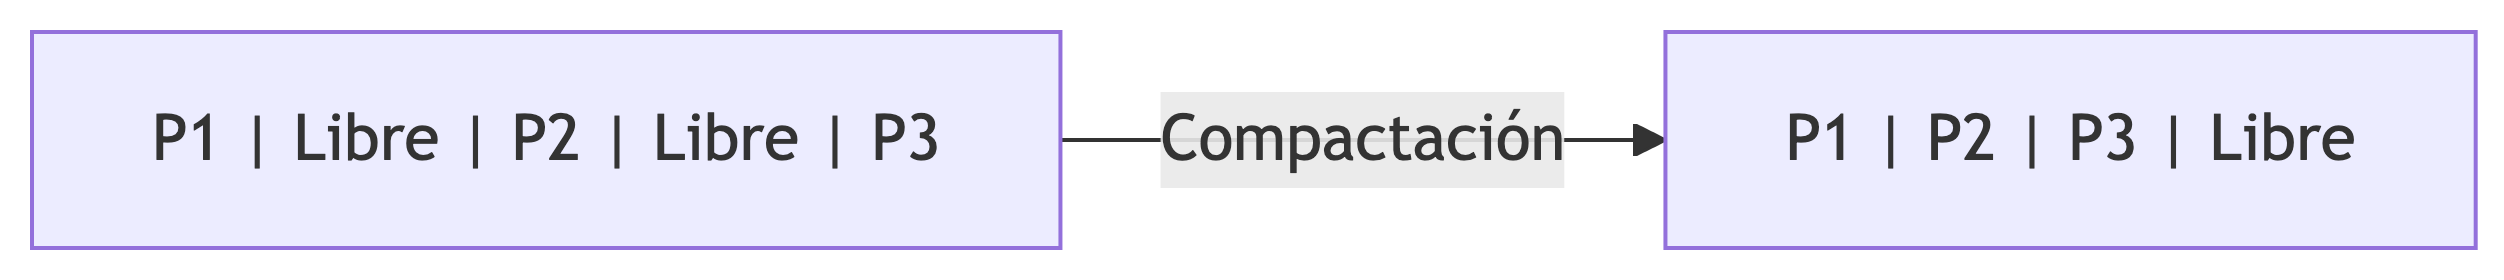
\includegraphics[width=6.53in,height=0.73in]{capitulos/18_gestion_memoria_sistemas_multiprogramados_files/figure-latex/mermaid-figure-7.png}

La compactación puede recuperar un espacio contiguo útil, pero tiene un
costo: mover procesos implica copiar memoria y ajustar sus ubicaciones.
Por ello requiere mecanismos de relocación adecuados.

\section{10. Swapping}\label{swapping}

El \textbf{swapping} consiste en trasladar temporalmente un proceso
entre la memoria principal y un área de almacenamiento secundario para
liberar RAM y permitir la entrada de otro proceso.

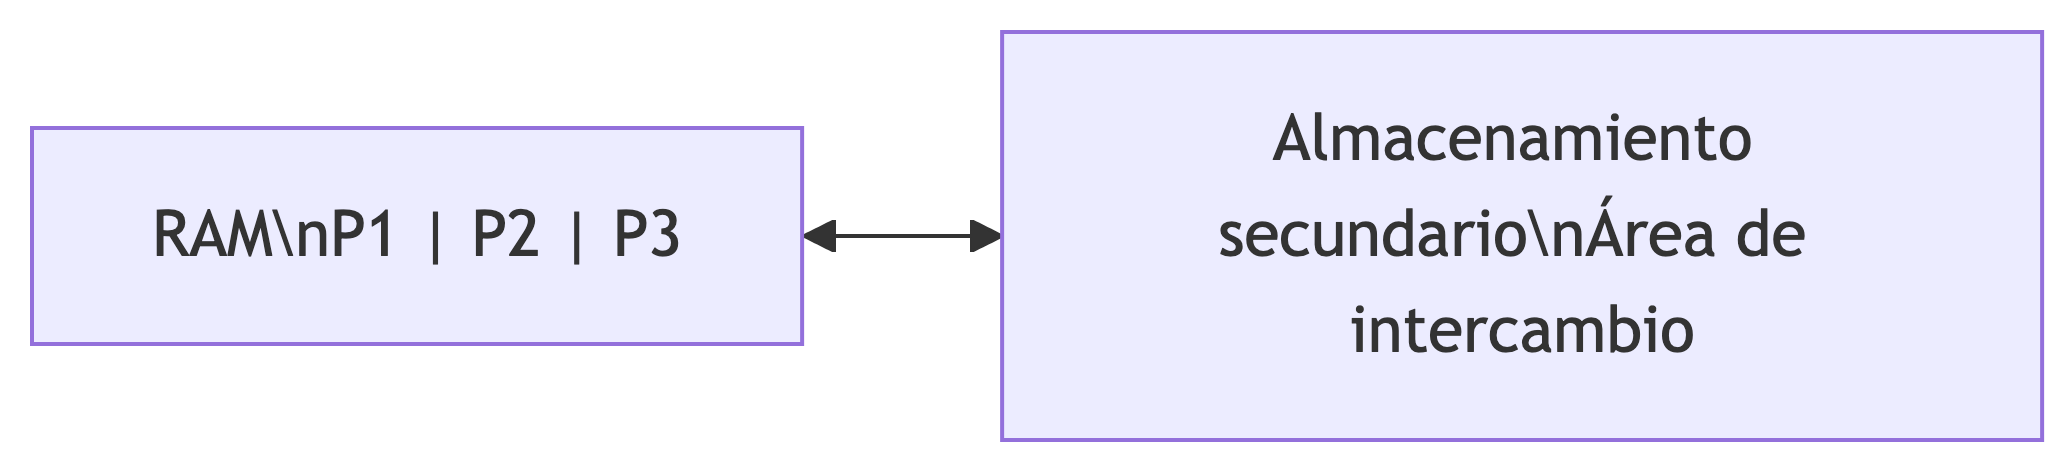
\includegraphics[width=5.4in,height=1.23in]{capitulos/18_gestion_memoria_sistemas_multiprogramados_files/figure-latex/mermaid-figure-6.png}

\subsection{Secuencia conceptual}\label{secuencia-conceptual}

\begin{enumerate}
\def\labelenumi{\arabic{enumi}.}
\tightlist
\item
  Se selecciona un proceso para suspenderlo.
\item
  Su estado/memoria se traslada al almacenamiento secundario.
\item
  Se libera su espacio en RAM.
\item
  Otro proceso puede ocupar el espacio disponible.
\item
  Cuando sea necesario, el proceso suspendido puede volver a memoria.
\end{enumerate}

\subsection{Ventajas y costos}\label{ventajas-y-costos}

{\def\LTcaptype{none} % do not increment counter
\begin{longtable}[]{@{}
  >{\raggedright\arraybackslash}p{(\linewidth - 2\tabcolsep) * \real{0.5000}}
  >{\raggedright\arraybackslash}p{(\linewidth - 2\tabcolsep) * \real{0.5000}}@{}}
\toprule\noalign{}
\begin{minipage}[b]{\linewidth}\raggedright
Ventajas
\end{minipage} & \begin{minipage}[b]{\linewidth}\raggedright
Costos o limitaciones
\end{minipage} \\
\midrule\noalign{}
\endhead
\bottomrule\noalign{}
\endlastfoot
Permite liberar RAM & Implica operaciones de E/S mucho más lentas que la
RAM \\
Aumenta la flexibilidad & Introduce latencia \\
Permite mantener más trabajo disponible para el sistema & Puede
interactuar con problemas de fragmentación \\
\end{longtable}
}

\section{11. Protección de memoria}\label{protecciuxf3n-de-memoria-1}

Cuando varios procesos comparten la RAM, ya no podemos permitir que uno
escriba libremente sobre el espacio de otro.

Un mecanismo conceptual sencillo utiliza un \textbf{registro base} y un
\textbf{registro límite}.

\begin{itemize}
\tightlist
\item
  \textbf{Base:} indica dónde comienza el espacio físico permitido para
  el proceso.
\item
  \textbf{Límite:} establece el rango válido que puede utilizar.
\end{itemize}

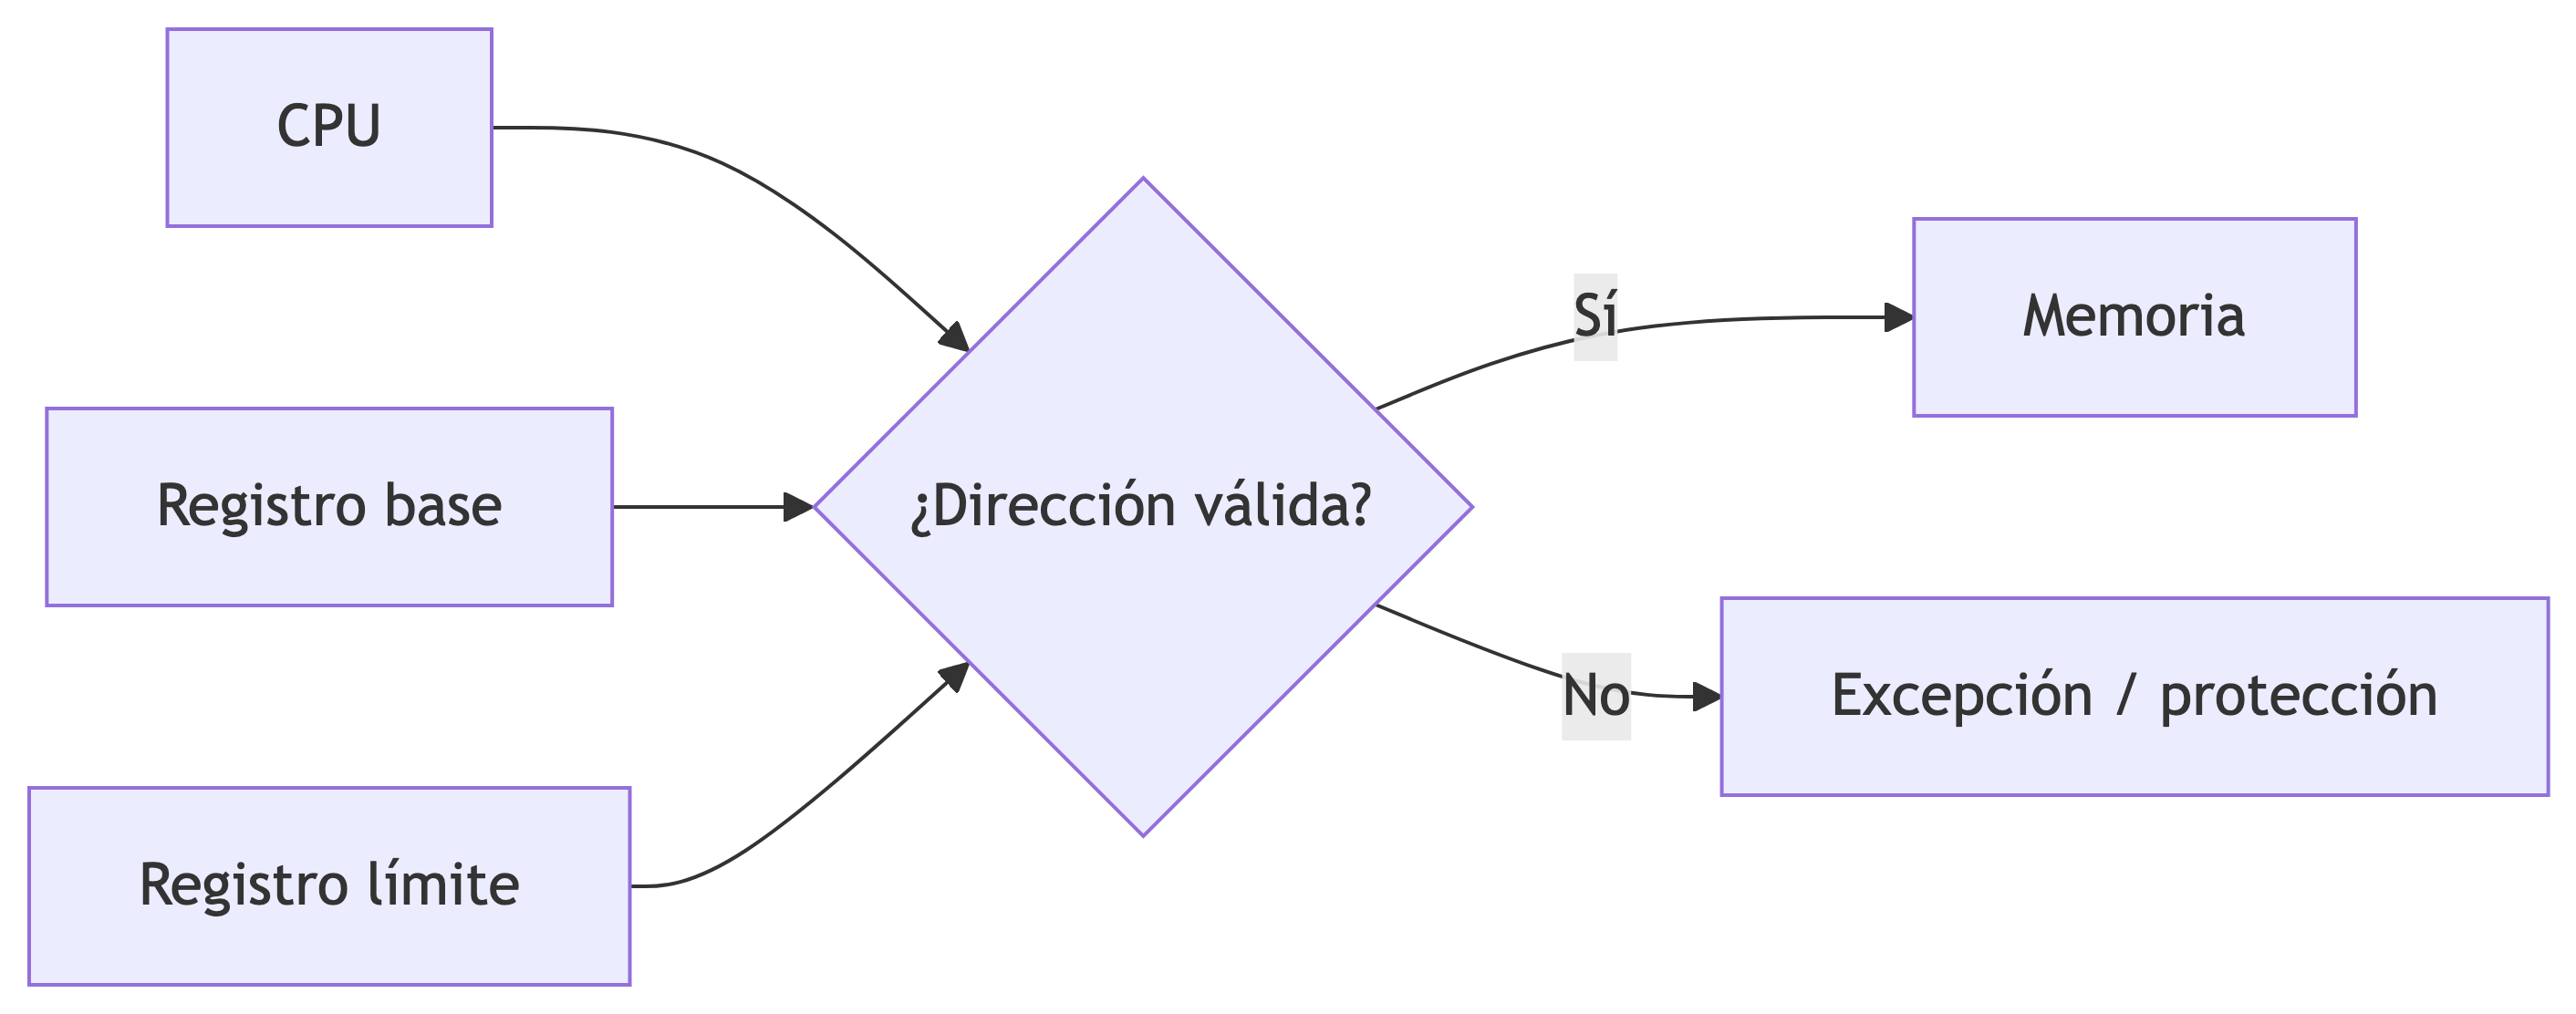
\includegraphics[width=7.36in,height=2.9in]{capitulos/18_gestion_memoria_sistemas_multiprogramados_files/figure-latex/mermaid-figure-5.png}

La protección es esencial: P1 no debe modificar accidentalmente el
código o los datos de P2 ni la memoria reservada para el sistema
operativo.

\section{12. Relocación dinámica}\label{relocaciuxf3n-dinuxe1mica}

En la Clase 17 vimos la \textbf{relocación estática}, donde el ajuste de
direcciones se realiza al cargar el programa.

En un sistema multiprogramado resulta útil que la traducción pueda
realizarse \textbf{durante la ejecución}. A esto lo llamamos
\textbf{relocación dinámica}.

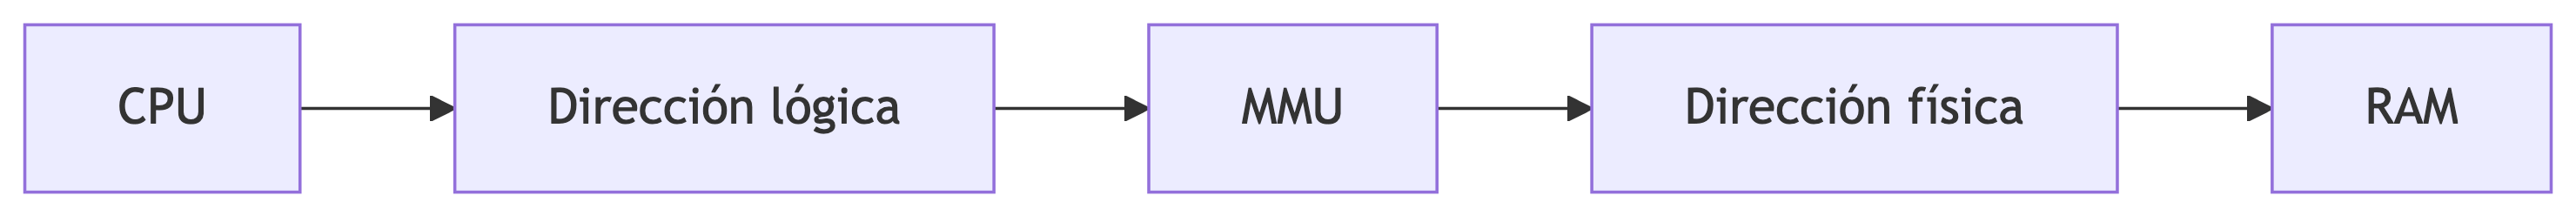
\includegraphics[width=8.67in,height=0.73in]{capitulos/18_gestion_memoria_sistemas_multiprogramados_files/figure-latex/mermaid-figure-4.png}

\section{13. ¿Qué es la MMU?}\label{quuxe9-es-la-mmu}

La \textbf{MMU (Memory Management Unit)} es el componente de hardware
encargado de participar en la traducción de las direcciones generadas
por la CPU hacia direcciones físicas de memoria.

En un modelo sencillo con base y desplazamiento:

\[
\text{Dirección física} = \text{Base} + \text{Dirección lógica}
\]

Supongamos:

\begin{itemize}
\tightlist
\item
  Base de P2 = 8000
\item
  Dirección lógica solicitada = 350
\end{itemize}

Entonces:

\[
8000 + 350 = 8350
\]

La CPU trabaja con la dirección lógica; el mecanismo de administración
de memoria permite llegar a la dirección física correspondiente.

\section{14. Memoria compartida}\label{memoria-compartida}

La protección mantiene separados a los procesos, pero algunas veces
\textbf{queremos que dos o más procesos compartan intencionalmente una
región de memoria}.

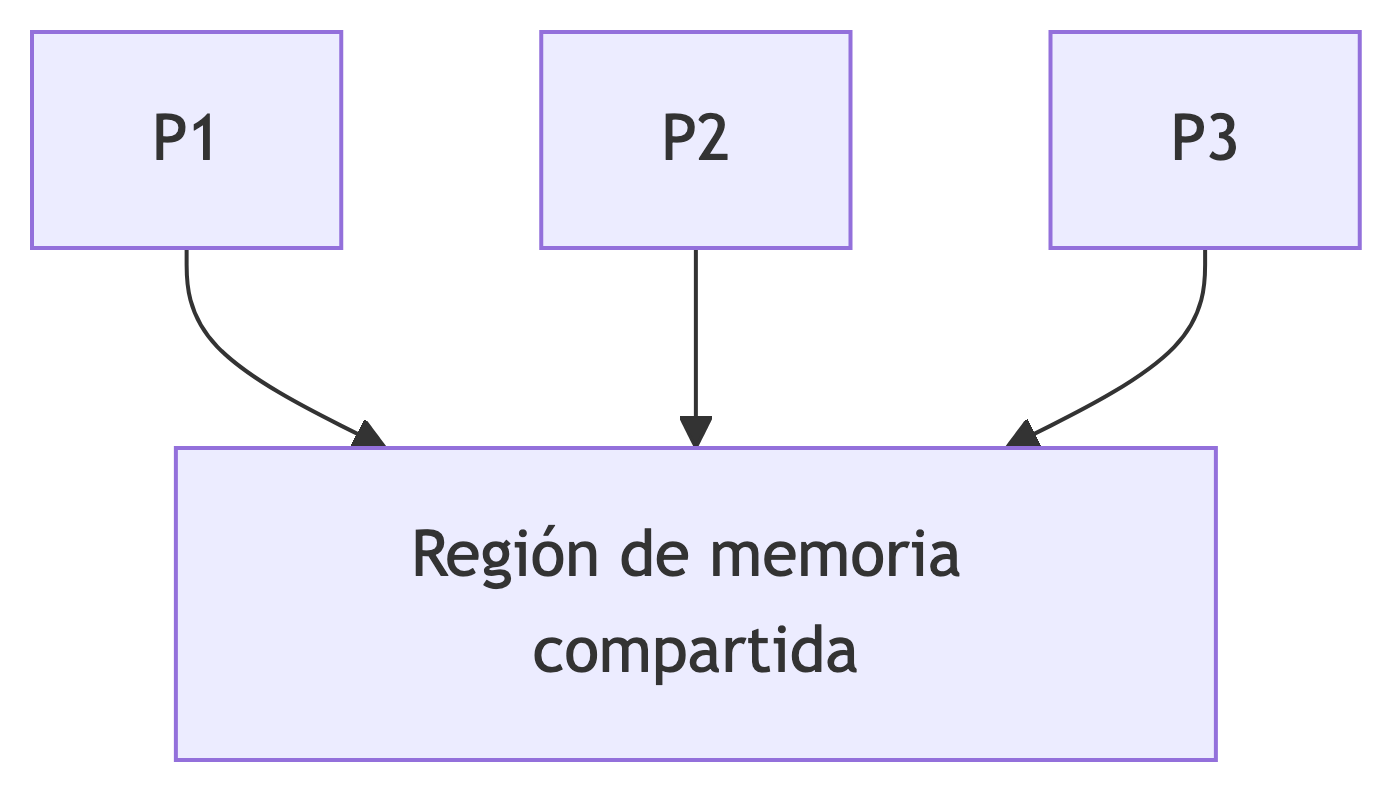
\includegraphics[width=3.62in,height=2.06in]{capitulos/18_gestion_memoria_sistemas_multiprogramados_files/figure-latex/mermaid-figure-3.png}

La memoria compartida puede utilizarse como mecanismo de
\textbf{comunicación entre procesos (IPC)} y para evitar duplicar
ciertos datos comunes.

Sin embargo, compartir memoria introduce un nuevo reto: los procesos
deben \textbf{sincronizar} sus accesos para evitar condiciones de
carrera y datos inconsistentes.

\begin{tcolorbox}[enhanced jigsaw, arc=.35mm, bottomrule=.15mm, bottomtitle=1mm, breakable, colback=white, colbacktitle=quarto-callout-note-color!10!white, colframe=quarto-callout-note-color-frame, coltitle=black, left=2mm, leftrule=.75mm, opacityback=0, opacitybacktitle=0.6, rightrule=.15mm, title=\textcolor{quarto-callout-note-color}{\faInfo}\hspace{0.5em}{Conexión con temas anteriores}, titlerule=0mm, toprule=.15mm, toptitle=1mm]

Aquí vuelven a aparecer conceptos como exclusión mutua, semáforos y
sincronización. La administración de memoria y la administración de
procesos están estrechamente relacionadas.

\end{tcolorbox}

\section{15. Comparación: monoprogramación y
multiprogramación}\label{comparaciuxf3n-monoprogramaciuxf3n-y-multiprogramaciuxf3n}

{\def\LTcaptype{none} % do not increment counter
\begin{longtable}[]{@{}
  >{\raggedright\arraybackslash}p{(\linewidth - 4\tabcolsep) * \real{0.3333}}
  >{\raggedright\arraybackslash}p{(\linewidth - 4\tabcolsep) * \real{0.3333}}
  >{\raggedright\arraybackslash}p{(\linewidth - 4\tabcolsep) * \real{0.3333}}@{}}
\toprule\noalign{}
\begin{minipage}[b]{\linewidth}\raggedright
Característica
\end{minipage} & \begin{minipage}[b]{\linewidth}\raggedright
Monoprogramación
\end{minipage} & \begin{minipage}[b]{\linewidth}\raggedright
Multiprogramación
\end{minipage} \\
\midrule\noalign{}
\endhead
\bottomrule\noalign{}
\endlastfoot
Programas/procesos de usuario residentes & Uno & Varios \\
Administración & Más sencilla & Más compleja \\
Aprovechamiento de CPU & Menor cuando el programa espera & Mayor al
alternar procesos \\
Protección entre procesos & No es el problema central & Fundamental \\
Relocación & Puede ser estática & Puede requerir mecanismos dinámicos \\
Fragmentación & Modelo sencillo & Puede aparecer interna o externa según
la técnica \\
\end{longtable}
}

\section{16. Caso integrador}\label{caso-integrador-3}

Disponemos de \textbf{1024 KB} de RAM. El sistema operativo ocupa
\textbf{200 KB}. El resto se administra mediante particiones dinámicas.

Se cargan:

\begin{itemize}
\tightlist
\item
  P1 = 200 KB
\item
  P2 = 150 KB
\item
  P3 = 180 KB
\end{itemize}

Después termina P2.

\subsection{Preguntas}\label{preguntas}

\begin{enumerate}
\def\labelenumi{\arabic{enumi}.}
\tightlist
\item
  Dibuja el estado de la memoria antes de que termine P2.
\item
  Dibuja el estado después de liberar P2.
\item
  ¿Qué tipo de fragmentación puede comenzar a observarse?
\item
  Si llega P4 de 140 KB, ¿puede utilizar el hueco dejado por P2?
\item
  ¿Cuánto espacio quedaría en ese hueco?
\item
  Si existen varios huecos, ¿qué información necesitarías para decidir
  el resultado de First Fit, Best Fit y Worst Fit?
\end{enumerate}

\section{17. Laboratorio conceptual: simulemos First
Fit}\label{laboratorio-conceptual-simulemos-first-fit}

Considera los huecos:

\begin{Shaded}
\begin{Highlighting}[]
\NormalTok{[120 KB] [60 KB] [300 KB] [180 KB]}
\end{Highlighting}
\end{Shaded}

Llegan, en orden:

\begin{Shaded}
\begin{Highlighting}[]
\NormalTok{P1 = 50 KB}
\NormalTok{P2 = 170 KB}
\NormalTok{P3 = 100 KB}
\end{Highlighting}
\end{Shaded}

Trabaja paso a paso:

\begin{enumerate}
\def\labelenumi{\arabic{enumi}.}
\tightlist
\item
  Asigna P1 usando First Fit.
\item
  Actualiza el tamaño del hueco restante.
\item
  Asigna P2.
\item
  Actualiza nuevamente la memoria.
\item
  Asigna P3.
\item
  Dibuja el estado final.
\end{enumerate}

\begin{quote}
No busques solamente el resultado. El objetivo es comprender que
\textbf{cada asignación modifica el conjunto de huecos disponibles para
la siguiente decisión}.
\end{quote}

\section{18. Puente hacia las siguientes
clases}\label{puente-hacia-las-siguientes-clases}

Hasta aquí hemos intentado mantener cada proceso en \textbf{un bloque
contiguo}. Esto genera una pregunta muy importante:

\begin{quote}
¿Es realmente necesario que todo el proceso esté almacenado en
posiciones consecutivas de memoria física?
\end{quote}

La respuesta conduce a las siguientes clases del libro:

\begin{itemize}
\tightlist
\item
  \textbf{Clase 19: Asignación de memoria contigua} - profundizaremos en
  las técnicas, criterios y problemas de la asignación contigua.
\item
  \textbf{Clase 20: Asignación de memoria no contigua} - estudiaremos
  cómo dividir un proceso y distribuir sus partes en distintas regiones
  de memoria.
\end{itemize}

Así, las clases 17 y 18 establecen el \textbf{contexto de gestión de
memoria}, mientras que las clases 19 y 20 desarrollan las
\textbf{técnicas de asignación} con mayor profundidad.

\section{19. Resumen}\label{resumen-2}

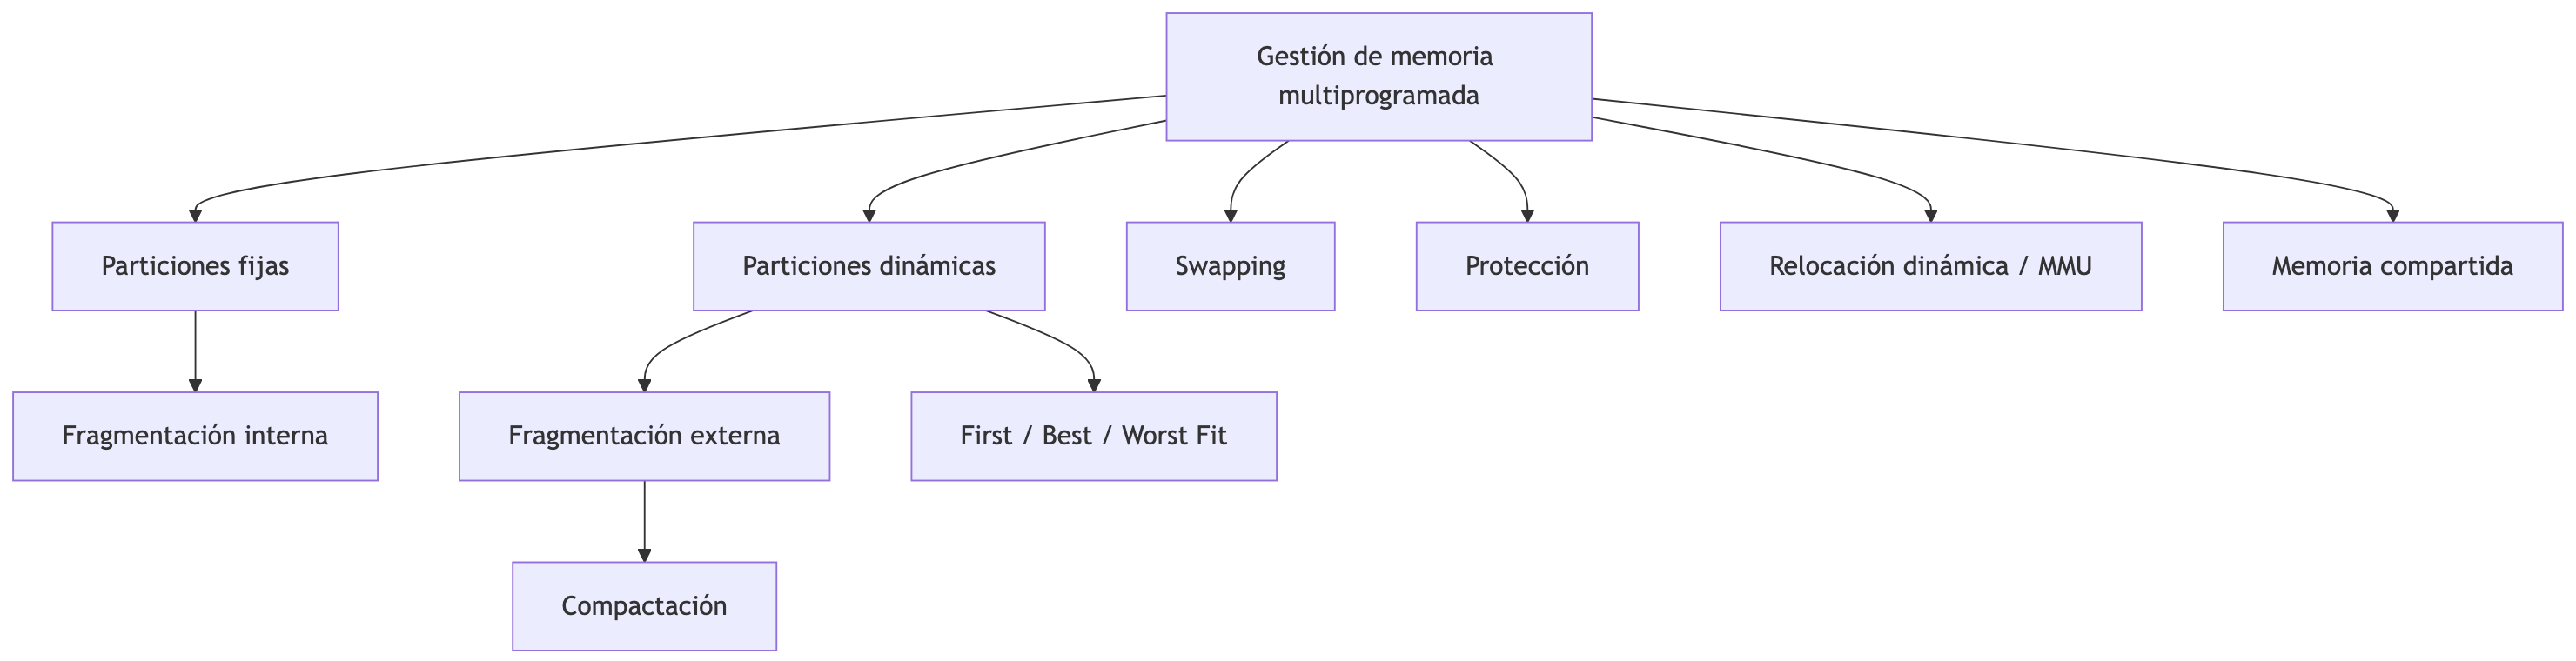
\includegraphics[width=16.41in,height=4.23in]{capitulos/18_gestion_memoria_sistemas_multiprogramados_files/figure-latex/mermaid-figure-2.png}

\subsection{Lo que debes llevarte de esta
clase}\label{lo-que-debes-llevarte-de-esta-clase-1}

\begin{itemize}
\tightlist
\item
  La multiprogramación mantiene varios procesos en memoria para
  aprovechar mejor la CPU.
\item
  Las particiones fijas pueden producir fragmentación interna.
\item
  Las particiones dinámicas pueden producir fragmentación externa.
\item
  First Fit, Best Fit y Worst Fit representan diferentes estrategias
  para seleccionar huecos libres.
\item
  La compactación reúne espacio libre disperso, pero requiere mover
  procesos.
\item
  El swapping permite liberar temporalmente RAM trasladando procesos al
  almacenamiento secundario.
\item
  La protección evita que un proceso interfiera con otro.
\item
  La MMU permite traducir direcciones durante la ejecución.
\item
  La memoria compartida permite comunicación eficiente, pero requiere
  sincronización.
\end{itemize}

\section{20. Autoevaluación}\label{autoevaluaciuxf3n-12}

\begin{enumerate}
\def\labelenumi{\arabic{enumi}.}
\tightlist
\item
  ¿Por qué la multiprogramación puede aumentar el aprovechamiento de la
  CPU?
\item
  ¿Cuál es la diferencia entre una partición fija y una dinámica?
\item
  ¿Qué es fragmentación interna?
\item
  ¿Qué es fragmentación externa?
\item
  ¿Qué hueco selecciona First Fit?
\item
  ¿Qué hueco selecciona Best Fit?
\item
  ¿Qué hueco selecciona Worst Fit?
\item
  ¿Qué problema intenta resolver la compactación?
\item
  ¿Qué significa swapping?
\item
  ¿Por qué se necesita protección de memoria en multiprogramación?
\item
  ¿Qué función cumple la MMU?
\item
  ¿Qué diferencia existe entre relocación estática y dinámica?
\item
  ¿Para qué puede utilizarse memoria compartida?
\item
  ¿Por qué la memoria compartida necesita mecanismos de sincronización?
\item
  ¿Qué problema de la asignación contigua prepara el camino hacia la
  asignación no contigua?
\end{enumerate}

\bookmarksetup{startatroot}

\chapter{Cierre de la clase}\label{cierre-de-la-clase-1}

\begin{tcolorbox}[enhanced jigsaw, arc=.35mm, bottomrule=.15mm, bottomtitle=1mm, breakable, colback=white, colbacktitle=quarto-callout-tip-color!10!white, colframe=quarto-callout-tip-color-frame, coltitle=black, left=2mm, leftrule=.75mm, opacityback=0, opacitybacktitle=0.6, rightrule=.15mm, title=\textcolor{quarto-callout-tip-color}{\faLightbulb}\hspace{0.5em}{Consejo final del Ingeniero}, titlerule=0mm, toprule=.15mm, toptitle=1mm]

Comprender un sistema operativo no consiste solamente en aprender
nombres de versiones o comandos. Consiste en comprender cómo se
administran recursos, cómo se protegen los procesos y cómo se construye
el entorno donde funcionan las aplicaciones.

\end{tcolorbox}

\section{Próximo paso}\label{pruxf3ximo-paso}

En la siguiente clase profundizaremos en la estructura y los componentes
de un sistema operativo, relacionando kernel, procesos, memoria,
dispositivos y servicios.


\backmatter


\end{document}
